\documentclass[aspectratio=169,9pt]{beamer}

% --- Theme: clean, robust (no external fonts, compiles with tectonic) ---
\usetheme{default}
\usecolortheme{seahorse}
\usefonttheme[onlymath]{serif}
\setbeamertemplate{navigation symbols}{}
\setbeamertemplate{itemize items}[circle]
\setbeamerfont{frametitle}{series=\bfseries}

\definecolor{accent}{RGB}{176,48,82}
\definecolor{ink}{RGB}{40,40,45}
\definecolor{soft}{RGB}{120,120,128}
\definecolor{good}{RGB}{30,110,70}
\definecolor{argA}{RGB}{40,95,165}
\definecolor{argB}{RGB}{190,140,20}
\definecolor{argC}{RGB}{125,60,150}
\setbeamercolor{frametitle}{fg=accent}
\setbeamercolor{structure}{fg=accent}
\setbeamercolor{normal text}{fg=ink}

\usepackage{amsmath,amssymb}
\usepackage{tikz}
\usetikzlibrary{arrows.meta,positioning,fit,backgrounds,calc,decorations.pathreplacing,patterns}
\usepackage{booktabs}
\usepackage{colortbl}
\usepackage{eqparbox}

\tikzset{
  box/.style={draw=accent!70, rounded corners, thick, fill=accent!6,
              inner sep=4pt, font=\scriptsize, align=center, minimum height=7mm},
  gate/.style={draw=soft, rounded corners, thin, fill=black!3,
              inner sep=3pt, font=\scriptsize, align=center},
  ghost/.style={draw=soft!60, rounded corners, thin, fill=black!2,
              inner sep=4pt, font=\scriptsize, align=center, minimum height=7mm, text=soft},
  flow/.style={-{Stealth[length=2mm]}, accent!80, thick},
}

\newcommand{\pending}[2][10.8cm]{%
  \begin{center}
  \begin{tikzpicture}
    \node[draw=soft, dashed, thick, rounded corners, fill=black!2,
          text width=#1, align=center, inner sep=7pt, font=\scriptsize]
      {\textbf{\textcolor{soft}{PENDING --- }}\textcolor{soft}{#2}};
  \end{tikzpicture}
  \end{center}}

\newcommand{\act}[2]{%
  \begin{frame}[plain]
    \centering \vfill
    {\Large\bfseries\color{accent} #1}\\[4pt]
    {\small #2}
    \vfill
  \end{frame}}

\newcommand{\subact}[2]{%
  \begin{frame}[plain]
    \centering \vfill
    {\large\bfseries\color{accent} #1}\\[4pt]
    {\small\color{soft} #2}
    \vfill
  \end{frame}}

\newcommand{\redlast}[1]{\multicolumn{1}{>{\columncolor{accent!14}[\tabcolsep][0pt]}c@{}}{#1}}
\newcommand{\seedtag}{g}
\newcommand{\seedpm}[2]{\eqmakebox[\seedtag M][r]{#1}\,{\tiny\color{soft}$\pm$\eqmakebox[\seedtag S][l]{#2}}}
\newcommand{\tintlast}[2]{\multicolumn{1}{>{\columncolor{#1}[\tabcolsep][0pt]}c@{}}{#2}}
\newcommand{\hleq}[1]{{\setlength{\fboxsep}{1.5pt}\colorbox{accent!12}{$\displaystyle #1$}}}
\newcommand{\hlval}[2]{{\setlength{\fboxsep}{1.2pt}\colorbox{#1}{\textcolor{white}{#2}}}}
\newcommand{\tintfirst}[2]{\multicolumn{1}{@{}>{\columncolor{#1}[0pt][0pt]}l}{#2\hspace{5pt}}}
\newcommand{\denomhl}[1]{{\setlength{\fboxsep}{1.5pt}\colorbox{accent!14}{$#1$}}}


\title{\textbf{DLR-TomoSAR --- The Full Project}}
\subtitle{Amortising tomographic inversion with deep networks:\\ from per-pixel fitting to physics-constrained learning}
\date{\small July 2026}
\author{}

\begin{document}

% ---------------------------------------------------------------- 1 Title
\begin{frame}[plain]
  \titlepage
  \vspace{-1.2em}
  \centering
  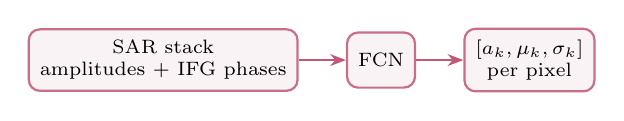
\begin{tikzpicture}[node distance=6mm]
    \node[box] (in)  {SAR stack\\{\scriptsize amplitudes + IFG phases}};
    \node[box, right=of in] (net) {FCN};
    \node[box, right=of net] (out) {$[a_k,\mu_k,\sigma_k]$\\per pixel};
    \draw[flow] (in) -- (net);
    \draw[flow] (net) -- (out);
  \end{tikzpicture}
  \\[2pt]
  {\scriptsize One forward pass replaces per-pixel nonlinear fitting of the elevation spectrum.}
\end{frame}

% ---------------------------------------------------------------- 2 Outline
\begin{frame}{Outline}
  \small
  \begin{enumerate}
    \item \textbf{Problem} --- the tomographic elevation spectrum and its per-pixel cost
    \item \textbf{Data \& ground truth} --- F-SAR stack, GPU-scale label generation, normalization
    \item \textbf{Method} --- set matching, slot imbalance, training stability
    \item \textbf{What does the network need?} --- context ladder, patch sizes, input ablation
    \item \textbf{Benchmark} --- every backbone $\times$ every objective, one winner
    \item \textbf{Physics-constrained losses} --- five terms, curriculum \hfill {\color{soft}(in progress)}
    \item \textbf{JEPA pretraining} --- predicting profile embeddings \hfill {\color{soft}(in progress)}
  \end{enumerate}
\end{frame}

% ---------------------------------------------------------------- 3 What this project does
\begin{frame}{What this project does}
  \centering
  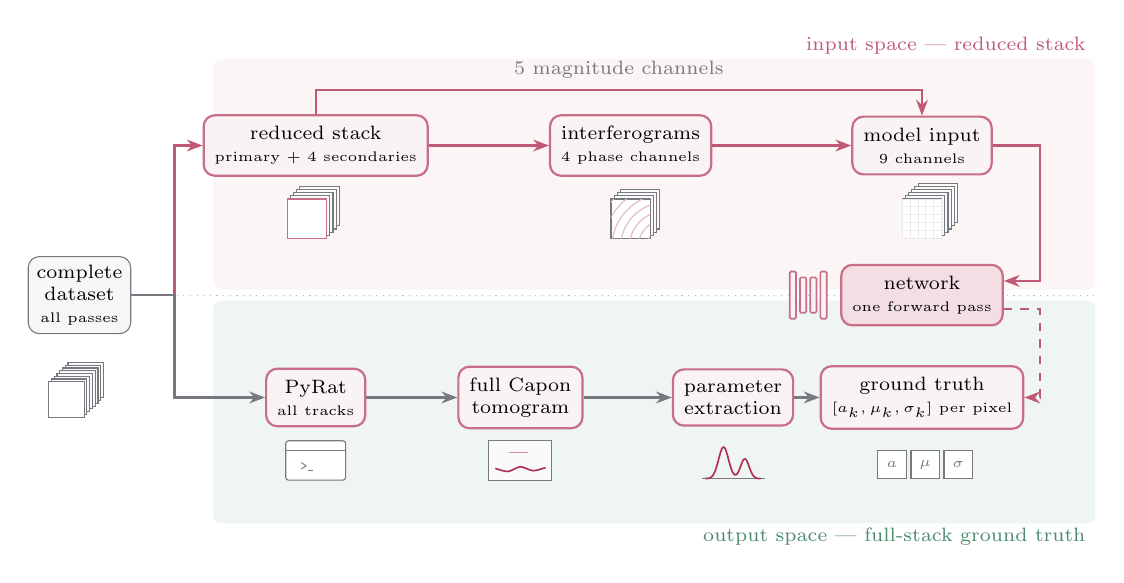
\begin{tikzpicture}
    \begin{scope}[on background layer]
      \fill[accent!5,rounded corners=3pt] (1.7,0.07) rectangle (12.9,3.0);
      \fill[good!7,rounded corners=3pt] (1.7,-0.07) rectangle (12.9,-2.9);
      \draw[soft!50,dotted] (-0.2,0) -- (12.9,0);
    \end{scope}
    \node[font=\scriptsize,text=accent!80,anchor=east] at (12.9,3.17) {input space --- reduced stack};
    \node[font=\scriptsize,text=good!80,anchor=east] at (12.9,-3.07) {output space --- full-stack ground truth};
    \node[gate] (ds) at (0,0) {complete\\dataset\\{\tiny all passes}};
    \foreach \i in {7,6,5,4,3,2,1} \draw[soft,thin,fill=black!2] (-0.39+0.035*\i,-1.55+0.035*\i) rectangle ++(0.45,0.45);
    \draw[soft,thin,fill=white] (-0.39,-1.55) rectangle ++(0.45,0.45);
    \node[box] (top1) at (3.0,1.9) {reduced stack\\{\tiny primary + 4 secondaries}};
    \foreach \i in {4,3,2,1} \draw[soft,thin,fill=black!2] (2.64+0.04*\i,0.72+0.04*\i) rectangle ++(0.5,0.5);
    \draw[accent!70,thin,fill=white] (2.64,0.72) rectangle ++(0.5,0.5);
    \node[box] (top2) at (7.0,1.9) {interferograms\\{\tiny 4 phase channels}};
    \foreach \i in {3,2,1} \draw[soft,thin,fill=black!2] (6.75+0.04*\i,0.72+0.04*\i) rectangle ++(0.5,0.5);
    \draw[soft,thin,fill=white] (6.75,0.72) rectangle ++(0.5,0.5);
    \begin{scope} \clip (6.75,0.72) rectangle ++(0.5,0.5); \foreach \r in {0.25,0.36,...,0.95} \draw[accent!35,thin] (7.45,0.6) circle (\r); \end{scope}
    \node[box] (top3) at (10.7,1.9) {model input\\{\tiny 9 channels}};
    \foreach \i in {5,4,3,2,1} \draw[soft,thin,fill=black!2] (10.45+0.04*\i,0.72+0.04*\i) rectangle ++(0.5,0.5);
    \draw[soft,thin,fill=white] (10.45,0.72) rectangle ++(0.5,0.5);
    \draw[black!8,step=0.1,shift={(10.45,0.72)}] (0,0) grid (0.5,0.5);
    \node[box, fill=accent!16] (net) at (10.7,0) {network\\{\tiny one forward pass}};
    \foreach \x/\h in {9.02/0.6,9.15/0.45,9.28/0.45,9.41/0.6} \draw[accent!70,semithick,fill=accent!6,rounded corners=0.5pt] (\x,-\h/2) rectangle ++(0.08,\h);
    \node[box] (bot1) at (3.0,-1.3) {PyRat\\{\tiny all tracks}};
    \draw[soft,thin,rounded corners=1pt,fill=white] (2.62,-2.35) rectangle ++(0.76,0.5);
    \draw[soft,thin] (2.62,-1.97) -- (3.38,-1.97);
    \node[font=\tiny,text=soft,anchor=west] at (2.68,-2.18) {\texttt{>\_}};
    \node[box] (bot2) at (5.6,-1.3) {full Capon\\tomogram};
    \draw[soft,thin,fill=black!2] (5.2,-2.35) rectangle ++(0.8,0.5);
    \draw[accent,semithick] plot[smooth] coordinates {(5.28,-2.20) (5.44,-2.24) (5.60,-2.18) (5.76,-2.23) (5.92,-2.19)};
    \draw[accent!55,semithick] (5.45,-2.00) -- (5.70,-2.00);
    \node[box] (bot3) at (8.3,-1.3) {parameter\\extraction};
    \draw[soft,thin] (7.9,-2.33) -- (8.7,-2.33);
    \draw[accent,semithick] plot[domain=7.95:8.65,samples=60] (\x,{-2.33+0.4*exp(-(\x-8.18)^2/0.008)+0.25*exp(-(\x-8.45)^2/0.006)});
    \node[box] (gt) at (10.7,-1.3) {ground truth\\{\tiny $[a_k,\mu_k,\sigma_k]$ per pixel}};
    \foreach \x/\lbl in {10.14/{$a$},10.56/{$\mu$},10.98/{$\sigma$}} { \draw[soft,thin,fill=white] (\x,-2.33) rectangle ++(0.36,0.36); \node[font=\tiny,text=soft] at (\x+0.18,-2.15) {\lbl}; }
    \draw[flow] (ds.east) -- ++(0.55,0) |- (top1.west);
    \draw[flow, soft] (ds.east) -- ++(0.55,0) |- (bot1.west);
    \draw[flow] (top1) -- (top2);
    \draw[flow] (top2) -- (top3);
    \draw[flow] (top1.north) -- (3.0,2.6) -- (10.7,2.6) -- (top3.north);
    \node[font=\scriptsize,text=soft,anchor=south] at (6.85,2.63) {5 magnitude channels};
    \draw[flow] (top3.east) -| (12.2,0.18) -- ([yshift=0.18cm]net.east);
    \draw[flow, soft] (bot1) -- (bot2);
    \draw[flow, soft] (bot2) -- (bot3);
    \draw[flow, soft] (bot3) -- (gt);
    \draw[flow, dashed] ([yshift=-0.18cm]net.east) -- (12.2,-0.18) |- (gt.east);
  \end{tikzpicture}
  \\[8pt]
  \small
  A network learns to reconstruct, from the \textbf{reduced} stack alone,\\
  the per-pixel profile parameters that the full-stack tomogram and classical fit produce.
\end{frame}

% ---------------------------------------------------------------- Legacy -> current, model and objective
\begin{frame}{From the legacy pipeline to the current system: model and objective}
  \centering
  \scriptsize
  \renewcommand{\arraystretch}{1.22}
  \begin{tabular}{@{}p{2.5cm} p{4.9cm} p{5.9cm}@{}}
    \toprule
    & \textbf{legacy pipeline} & \textbf{current system} \\
    \midrule
    backbone
      & one fixed 5-level UNet (64\,$\to$\,1024, plain double conv, no normalization layers, no dropout)
      & registry of 20 backbones under one contract; standard trunk UNet-skip \\
    model form
      & single network, 6 output channels
      & dual model: parameter trunk + existence trunk, joint head, \hlval{accent}{90/10} loss split \\
    output head
      & single $1{\times}1$ conv
      & head axis: conv / multihead / per-Gaussian / \hlval{accent}{set prediction} ($K$ gated PixelMLP heads + existence gate) \\
    scatterer slots
      & exactly 2, fixed ground-first identity
      & $K$ slots (studied at $K{=}2$ and $K{=}5$); \hlval{accent}{Hungarian matching} assigns predictions to targets, sorted-GT kept as control \\
    presence
      & gated by the \emph{prediction} ($\hat a_2 > 10^{-4}$, $\hat w_2 \ge 0$); missed scatterers never penalised, slot collapse is a loss optimum
      & gated by the \emph{ground truth}; per-slot presence balancing + \hlval{accent}{active normalization}; collapse eliminated \\
    parameter loss
      & masked MSE on min-max targets, equal-weight group means
      & param L1 standard; Huber / MSE / curve reconstruction alternatives, benchmarked per backbone \\
    physics terms
      & \textcolor{soft}{absent}
      & coherence resynthesis, covariance matching, Capon cycle, moments, total power; warmup $\to$ complete curriculum \\
    \bottomrule
  \end{tabular}
\end{frame}

% ---------------------------------------------------------------- Legacy -> current, data and normalization
\begin{frame}{From the legacy pipeline to the current system: data and normalization}
  \centering
  \scriptsize
  \renewcommand{\arraystretch}{1.22}
  \begin{tabular}{@{}p{2.5cm} p{4.9cm} p{5.9cm}@{}}
    \toprule
    & \textbf{legacy pipeline} & \textbf{current system} \\
    \midrule
    input channels
      & 4 secondary amplitudes + 4 interferogram phases
      & + primary amplitude; per-group representation axis (magnitude / phase / real-imag), optional DEM \\
    input normalization
      & raw $\log(1+m)$ magnitudes; phases mapped $[-\pi,\pi] \to [0,1]$ by fixed constants
      & per-slot-kind strategies \hlval{accent}{fitted from the train region} (robust-IQR log1p for heavy-tailed magnitudes, z-score / fixed-$\pi$ phases), per-channel overrides \\
    target normalization
      & fixed hand-set min-max bounds per channel
      & fitted per-channel statistics over active pixels; heavy-tailed amplitude and width compressed by robust-IQR log1p \\
    output range
      & unconstrained regression
      & physical clamping of $\hat a, \hat\mu, \hat\sigma$ with leaky slopes \\
    data split
      & random patch shuffle 80/10/10; neighbouring patches leak across splits
      & contiguous azimuth bands for train / val / test \\
    patches
      & $64 \times 64$, square only
      & rectangular (azimuth, range) with per-axis stride, standard $64{\times}32$ / $32{\times}16$; optimum derived and confirmed by sweep \\
    augmentation
      & \textcolor{soft}{absent}
      & flips standard; rotation and noise as options, gains benchmarked \\
    \bottomrule
  \end{tabular}
\end{frame}

% ---------------------------------------------------------------- Legacy -> current, optimization and tooling
\begin{frame}{From the legacy pipeline to the current system: optimization and tooling}
  \centering
  \scriptsize
  \renewcommand{\arraystretch}{1.22}
  \begin{tabular}{@{}p{2.5cm} p{4.9cm} p{5.9cm}@{}}
    \toprule
    & \textbf{legacy pipeline} & \textbf{current system} \\
    \midrule
    optimizer
      & Adam, one parameter group, lr $10^{-5}$, no weight decay
      & AdamW with per-module groups (encoder / bottleneck / decoder / head each own lr and weight decay) \\
    schedule
      & constant lr, fixed 300 epochs
      & cosine annealing + \hlval{accent}{lr warmup}, batch-scaled lr, early stopping with best-checkpoint restore \\
    stabilization
      & \textcolor{soft}{absent}
      & \hlval{accent}{gradient clipping} (fixed and adaptive modes), overfit gate before every run, loss-scale probes, non-finite abort; EMA and AMP options \\
    checkpointing
      & one save after the last epoch
      & per-epoch validation, best + resumable trainer state, run manifests and completion markers \\
    evaluation
      & final MSE print on a held-out loader
      & benchmark suite over every backbone $\times$ objective, occupancy and count diagnostics, physical MAEs, leaderboard \\
    experiment control
      & hand-edited driver scripts
      & config-contract entry points, web console with run health, GPU pools and queueing, multi-seed fan-out \\
    reproducibility
      & \textcolor{soft}{absent}
      & one-click \hlval{good}{legacy mode} rebuilds the entire left column inside this stack for A/B comparison \\
    \bottomrule
  \end{tabular}
\end{frame}


\act{I \ \ Problem}{signal model \; $\cdot$ \; Gaussian mixture \; $\cdot$ \; amortisation}

% ---------------------------------------------------------------- 4 Signal model
\begin{frame}{The tomographic signal model}
  \setlength{\abovedisplayskip}{5pt}
  \setlength{\belowdisplayskip}{5pt}
  \setlength{\abovedisplayshortskip}{3pt}
  \setlength{\belowdisplayshortskip}{3pt}
  \begin{columns}[T]
    \begin{column}{0.55\textwidth}
      \small
      Each track's baseline $b_i$ sets its vertical wavenumber:
      \[
        k_z^{(i)} = \frac{4\pi\, b_i}{\lambda\, r_0\, \sin\theta}
      \]
      Each pixel is a Fourier sample of the reflectivity $u(z)$:
      \[
        g_i = \int u(z)\, e^{\,j\,k_z^{(i)} z}\, dz
      \]
      Coherences sample the spectrum of $p(z)=\mathrm{E}\,|u(z)|^2$:
      \[
        \gamma_{ij} \;=\; \frac{\int p(z)\, e^{\,j\,(k_z^{(i)}-k_z^{(j)})\, z}\, dz}{\int p(z)\, dz}
      \]
      Classical inversion scans $\mathbf{a}(z)$ over the sample covariance $\hat{\mathbf{R}}$:
      \par\vspace{7pt}
      \[
        \mathbf{a}(z)=\big[e^{\,j k_z^{(1)} z}\!,\dots,e^{\,j k_z^{(N)} z}\big]^{\top}
      \]
      \par\vspace{2pt}
      \[
        \hat p_{\mathrm{BF}}(z)=\tfrac{1}{N^2}\,\mathbf{a}^{\mathsf H}(z)\,\hat{\mathbf{R}}\,\mathbf{a}(z)
        \quad
        \hat p_{\mathrm{Capon}}(z)=\big[\mathbf{a}^{\mathsf H}(z)\,\hat{\mathbf{R}}^{-1}\,\mathbf{a}(z)\big]^{-1}
      \]
    \end{column}
    \begin{column}{0.43\textwidth}
      \centering
      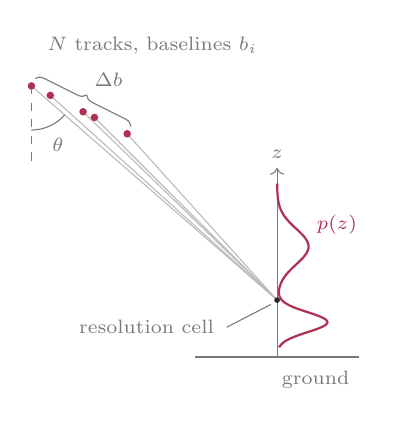
\begin{tikzpicture}[scale=0.8]
        \coordinate (cell) at (3.9,1.15);
        \foreach \p in {(0.00,4.55),(0.30,4.40),(0.82,4.14),(1.00,4.05),(1.52,3.79)}
          \draw[soft!50, thin] \p -- (cell);
        \draw[soft, dashed, thin] (0,4.55) -- (0,3.35);
        \draw[soft, thin] (0,3.85) arc[start angle=-90, end angle=-41, radius=0.7];
        \node[font=\scriptsize, text=soft] at (0.42,3.62) {$\theta$};
        \foreach \p in {(0.00,4.55),(0.30,4.40),(0.82,4.14),(1.00,4.05),(1.52,3.79)}
          \fill[accent] \p circle (1.7pt);
        \draw[decorate, decoration={brace, amplitude=3pt, raise=3pt}, soft]
          (0.00,4.55) -- (1.52,3.79)
          node[midway, above right=5pt and 2pt, font=\scriptsize, text=soft] {$\Delta b$};
        \node[font=\scriptsize, text=soft, anchor=south west] at (0.10,4.90) {$N$ tracks, baselines $b_i$};
        \draw[soft, thick] (2.6,0.25) -- (5.2,0.25);
        \node[font=\scriptsize, text=soft, anchor=north east] at (5.2,0.18) {ground};
        \draw[->, soft] (3.9,0.25) -- (3.9,3.25) node[above, font=\scriptsize] {$z$};
        \draw[accent, thick, smooth, samples=60, domain=0.15:2.75, variable=\z]
          plot ({3.9+0.8*exp(-(\z-0.55)^2/0.05)+0.5*exp(-(\z-1.75)^2/0.16)},{0.25+\z});
        \fill[ink] (cell) circle (1.3pt);
        \node[font=\scriptsize, text=accent] at (4.85,2.35) {$p(z)$};
        \node[font=\scriptsize, text=soft, anchor=east] at (3.05,0.72) {resolution cell};
        \draw[soft, thin] (3.10,0.72) -- (3.80,1.08);
      \end{tikzpicture}
      \\[1pt]
      {\scriptsize The aperture $\Delta b$ sets the Rayleigh resolution
       $\delta_z = \lambda r_0 \sin\theta / (2\Delta b)$.}
      \\[8pt]
      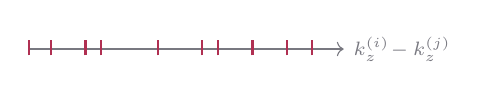
\begin{tikzpicture}[scale=0.8]
        \draw[->, soft] (0,0) -- (5.0,0) node[right, font=\scriptsize] {$k_z^{(i)}\!-k_z^{(j)}$};
        \foreach \x in {0.0,0.35,0.9,1.15,2.05,2.75,3.0,3.55,4.1,4.5}
          \draw[accent, thick] (\x,-0.1) -- (\x,0.15);
      \end{tikzpicture}
      \\[1pt]
      {\scriptsize Finite, irregular sampling of the Fourier axis ---\\
       tomography inverts it back to $p(z)$.}
    \end{column}
  \end{columns}
\end{frame}

% ---------------------------------------------------------------- 5 Gaussian mixture
\begin{frame}{Parameterising the spectrum --- and its classical cost}
  \setlength{\abovedisplayskip}{4pt}
  \setlength{\belowdisplayskip}{4pt}
  \begin{columns}[T]
    \begin{column}{0.52\textwidth}
      \small
      The elevation power spectrum at each pixel is modelled as a $K$-Gaussian mixture:
      \[
        p(z)=\sum_{k=1}^{K} a_k\,\exp\!\Big(\!-\tfrac{(z-\mu_k)^2}{2\sigma_k^2}\Big)
      \]
      \begin{center}
      \begin{tabular}{@{}r@{\hskip 8pt}l@{}}
        $a_k$      & backscattered power of scatterer $k$ \\
        $\mu_k$    & its elevation in the cell            \\
        $\sigma_k$ & its vertical spread                  \\
      \end{tabular}
      \end{center}
      \vspace{1pt}
      {\footnotesize Working configuration: $K{=}2$ --- covers 93.9\% of active pixels;
       the $K{=}5$ extension for the multi-scatterer tail is in development.}
    \end{column}
    \begin{column}{0.46\textwidth}
      \centering
      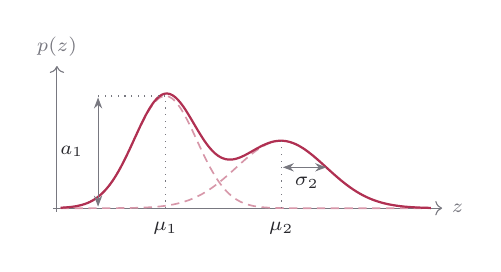
\begin{tikzpicture}[scale=0.95]
        \draw[->,soft] (-0.05,0) -- (5.15,0) node[right,font=\scriptsize]{$z$};
        \draw[->,soft] (0,-0.05) -- (0,1.9) node[above,font=\scriptsize]{$p(z)$};
        \draw[accent!50,semithick,densely dashed,domain=0.05:5.0,samples=90,smooth]
          plot (\x,{1.50*exp(-(\x-1.45)^2/(2*0.42*0.42))});
        \draw[accent!50,semithick,densely dashed,domain=0.05:5.0,samples=90,smooth]
          plot (\x,{0.90*exp(-(\x-3.00)^2/(2*0.60*0.60))});
        \draw[accent,thick,domain=0.05:5.0,samples=140,smooth]
          plot (\x,{1.50*exp(-(\x-1.45)^2/(2*0.42*0.42)) + 0.90*exp(-(\x-3.00)^2/(2*0.60*0.60))});
        \draw[soft,dotted] (1.45,0) -- (1.45,1.50);
        \draw[soft,dotted] (1.45,1.50) -- (0.55,1.50);
        \draw[{Stealth[length=1.4mm]}-{Stealth[length=1.4mm]},soft,thin] (0.55,0.02) -- (0.55,1.48);
        \node[font=\scriptsize,text=ink,anchor=east] at (0.48,0.76) {$a_1$};
        \node[font=\scriptsize,text=ink,anchor=north] at (1.45,-0.06) {$\mu_1$};
        \draw[soft,dotted] (3.00,0) -- (3.00,0.90);
        \node[font=\scriptsize,text=ink,anchor=north] at (3.00,-0.06) {$\mu_2$};
        \draw[{Stealth[length=1.4mm]}-{Stealth[length=1.4mm]},soft,thin] (3.02,0.546) -- (3.60,0.546);
        \node[font=\scriptsize,text=ink] at (3.34,0.34) {$\sigma_2$};
      \end{tikzpicture}
      \\[1pt]
      {\scriptsize \textcolor{accent}{Mixture $p(z)$} and its
       \textcolor{accent!60}{components (dashed)} --- three numbers per scatterer
       describe the whole profile.}
    \end{column}
  \end{columns}
  \vspace{16pt}
  \centering
  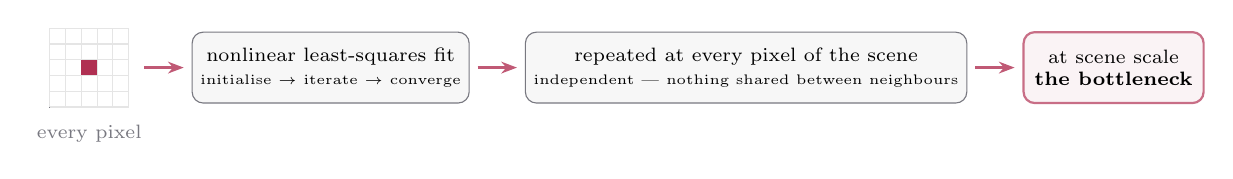
\begin{tikzpicture}
    \draw[soft,thin,fill=white] (0,-0.5) rectangle ++(1.0,1.0);
    \draw[black!10,step=0.2,shift={(0,-0.5)}] (0,0) grid (1.0,1.0);
    \fill[accent] (0.4,-0.1) rectangle ++(0.2,0.2);
    \node[font=\scriptsize,text=soft,anchor=north] at (0.5,-0.6) {every pixel};
    \draw[flow] (1.2,0) -- (1.7,0);
    \node[gate,anchor=west,minimum height=9mm] (fit) at (1.8,0)
      {nonlinear least-squares fit\\{\tiny initialise $\to$ iterate $\to$ converge}};
    \draw[flow] (fit.east) ++(0.1,0) -- ++(0.5,0);
    \node[gate,anchor=west,minimum height=9mm] (rep) at ([xshift=7mm]fit.east)
      {repeated at every pixel of the scene\\{\tiny independent --- nothing shared between neighbours}};
    \draw[flow] (rep.east) ++(0.1,0) -- ++(0.5,0);
    \node[box,anchor=west,minimum height=9mm] (btl) at ([xshift=7mm]rep.east)
      {at scene scale\\\textbf{the bottleneck}};
  \end{tikzpicture}
  \\[2pt]
  {\scriptsize The classical route restarts an iterative fit at every pixel ---
   the cost the amortised network removes (next).}
\end{frame}

% ---------------------------------------------------------------- 6 Amortisation
\begin{frame}{The amortisation idea}
  \small
  Train a fully-convolutional network to emit all $3K$ parameters directly,
  for every pixel of a patch at once:
  \[
    f_\theta:\ \mathbb{R}^{C_\text{in}\times P\times P}\ \longrightarrow\ \mathbb{R}^{3K\times P\times P}
  \]
  \begin{center}
  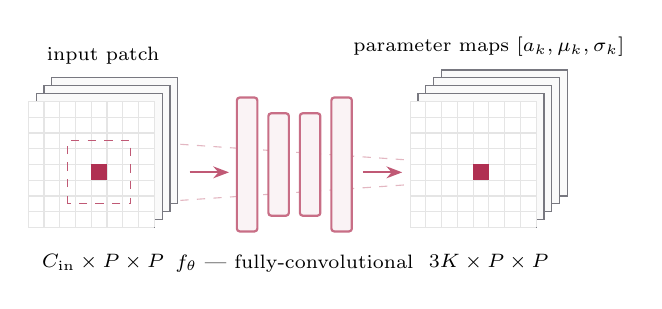
\begin{tikzpicture}
    \begin{scope}[on background layer]
      \draw[accent!35,dashed,thin] (1.3,1.1) -- (5.65,0.8);
      \draw[accent!35,dashed,thin] (1.3,0.3) -- (5.65,0.6);
    \end{scope}
    \foreach \i in {3,2,1} \draw[soft,thin,fill=black!2] (0.1*\i,0.1*\i) rectangle ++(1.6,1.6);
    \draw[soft,thin,fill=white] (0,0) rectangle (1.6,1.6);
    \draw[black!10,step=0.2] (0,0) grid (1.6,1.6);
    \fill[accent] (0.8,0.6) rectangle ++(0.2,0.2);
    \draw[accent!80,dashed,thin] (0.5,0.3) rectangle ++(0.8,0.8);
    \node[font=\scriptsize,anchor=south] at (0.95,1.95) {input patch};
    \node[font=\scriptsize,anchor=north] at (0.95,-0.22) {$C_\text{in}\times P\times P$};
    \draw[flow] (2.05,0.7) -- (2.55,0.7);
    \foreach \x/\h in {2.65/1.7,3.05/1.3,3.45/1.3,3.85/1.7}
      \draw[accent!70,thick,fill=accent!6,rounded corners=1pt] (\x,0.8-\h/2) rectangle ++(0.26,\h);
    \node[font=\scriptsize,anchor=north] at (3.38,-0.22) {$f_\theta$ --- fully-convolutional};
    \draw[flow] (4.25,0.7) -- (4.75,0.7);
    \foreach \i in {4,3,2,1} \draw[soft,thin,fill=black!2] (4.85+0.1*\i,0.1*\i) rectangle ++(1.6,1.6);
    \draw[soft,thin,fill=white] (4.85,0) rectangle ++(1.6,1.6);
    \draw[black!10,step=0.2,shift={(4.85,0)}] (0,0) grid (1.6,1.6);
    \fill[accent] (5.65,0.6) rectangle ++(0.2,0.2);
    \node[font=\scriptsize,anchor=south] at (5.85,2.05) {parameter maps $[a_k,\mu_k,\sigma_k]$};
    \node[font=\scriptsize,anchor=north] at (5.85,-0.22) {$3K\times P\times P$};
  \end{tikzpicture}
  \\[2pt]
  {\scriptsize \textcolor{accent}{One pixel}'s parameters draw on its
   \textcolor{accent!80}{spatial context window (dashed)}; the whole patch is decoded in a single pass.}
  \end{center}
  \begin{itemize}
    \item One forward pass replaces per-pixel iterative optimisation.
    \item The network sees a \textbf{spatial context window}, not an isolated pixel ---
          whether that context matters is a question the theory does not answer
          (Act IV measures it).
    \item Supervision: parameter maps produced by the classical fit (next act) ---
          with everything that implies about label quality (Act VI).
  \end{itemize}
\end{frame}


\act{II \ \ Data \& ground truth}{F-SAR stack \; $\cdot$ \; GPU label generation \; $\cdot$ \; heavy-tailed normalization}

% ---------------------------------------------------------------- 7 Stack & preprocessing
\begin{frame}{F-SAR stack and preprocessing}
  \begin{columns}[c]
    \begin{column}{0.42\textwidth}
      \small
      \begin{itemize}
        \item Airborne F-SAR stack over an urban test site; primary PS02, secondaries
              selected at training time (PS04/06/08/26) --- the \textbf{reduced stack}.
        \item Per-track acquisition geometry extracted from campaign metadata: per-pixel
              baselines, look angles, slant ranges (consumed by the physics losses, Act VI).
        \item Every artifact is written self-describing: config, stats and geometry ride
              with the data.
      \end{itemize}
    \end{column}
    \begin{column}{0.56\textwidth}
      \centering
      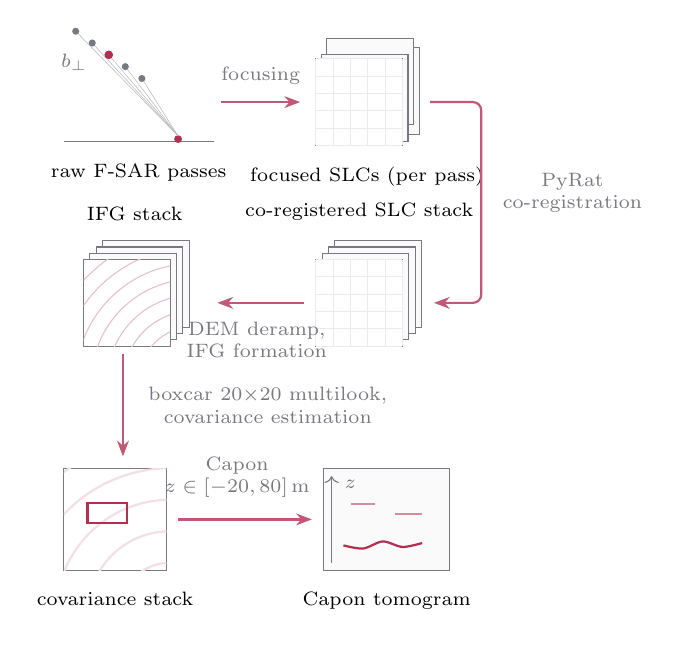
\begin{tikzpicture}
        \draw[soft,thin] (0,5.55) -- (1.9,5.55);
        \fill[accent] (1.45,5.58) circle (0.05);
        \foreach \x/\y in {0.15/6.95, 0.36/6.8, 0.78/6.5, 0.99/6.35} { \draw[soft!50,very thin] (\x,\y) -- (1.45,5.62); \fill[soft] (\x,\y) circle (0.045); }
        \draw[soft!50,very thin] (0.57,6.65) -- (1.45,5.62);
        \fill[accent] (0.57,6.65) circle (0.055);
        \node[font=\scriptsize,text=soft,anchor=east] at (0.42,6.55) {$b_\perp$};
        \node[font=\scriptsize,anchor=north] at (0.95,5.38) {raw F-SAR passes};
        \draw[flow] (2.0,6.05) -- (3.0,6.05);
        \node[font=\scriptsize,text=soft,anchor=south] at (2.5,6.15) {focusing};
        \draw[soft,thin,fill=black!2] (3.42,5.64) rectangle ++(1.1,1.1);
        \draw[soft,thin,fill=black!2] (3.34,5.76) rectangle ++(1.1,1.1);
        \draw[soft,thin,fill=black!2] (3.27,5.55) rectangle ++(1.1,1.1);
        \draw[soft,thin,fill=white] (3.2,5.5) rectangle ++(1.1,1.1);
        \draw[black!8,step=0.22,shift={(3.2,5.5)}] (0,0) grid (1.1,1.1);
        \node[font=\scriptsize,anchor=north] at (3.85,5.35) {focused SLCs (per pass)};
        \draw[flow,rounded corners=3pt] (4.65,6.05) -- (5.3,6.05) -- (5.3,3.5) -- (4.7,3.5);
        \node[font=\scriptsize,text=soft,align=center,anchor=west] at (5.45,4.9) {PyRat\\co-registration};
        \foreach \i in {3,2,1} \draw[soft,thin,fill=black!2] (3.2+0.08*\i,2.95+0.08*\i) rectangle ++(1.1,1.1);
        \draw[soft,thin,fill=white] (3.2,2.95) rectangle ++(1.1,1.1);
        \draw[black!8,step=0.22,shift={(3.2,2.95)}] (0,0) grid (1.1,1.1);
        \node[font=\scriptsize,anchor=south] at (3.75,4.42) {co-registered SLC stack};
        \draw[flow] (3.05,3.5) -- (1.95,3.5);
        \node[font=\scriptsize,text=soft,align=center,anchor=north] at (2.45,3.38) {DEM deramp,\\IFG formation};
        \foreach \i in {3,2,1} \draw[soft,thin,fill=black!2] (0.25+0.08*\i,2.95+0.08*\i) rectangle ++(1.1,1.1);
        \draw[soft,thin,fill=white] (0.25,2.95) rectangle ++(1.1,1.1);
        \begin{scope} \clip (0.25,2.95) rectangle ++(1.1,1.1); \foreach \r in {0.5,0.7,...,2.1} \draw[accent!30,thin] (1.65,2.5) circle (\r); \end{scope}
        \node[font=\scriptsize,anchor=south] at (0.9,4.42) {IFG stack};
        \draw[flow] (0.75,2.85) -- (0.75,1.55);
        \node[font=\scriptsize,text=soft,align=center,anchor=west] at (0.95,2.2) {boxcar $20{\times}20$ multilook,\\covariance estimation};
        \draw[soft,thin,fill=white] (0.0,0.1) rectangle ++(1.3,1.3);
        \begin{scope} \clip (0.0,0.1) rectangle ++(1.3,1.3); \foreach \r in {0.65,1.05,...,2.75} \draw[accent!15,thick] (1.35,-0.45) circle (\r); \end{scope}
        \draw[accent,thick] (0.3,0.7) rectangle ++(0.5,0.26);
        \node[font=\scriptsize,anchor=north] at (0.65,-0.05) {covariance stack};
        \draw[flow] (1.45,0.75) -- (3.15,0.75);
        \node[font=\scriptsize,text=soft,align=center,anchor=south] at (2.2,0.9) {Capon\\$z\in[-20,80]$\,m};
        \draw[soft,thin,fill=black!2] (3.3,0.1) rectangle ++(1.6,1.3);
        \draw[->,soft] (3.4,0.2) -- (3.4,1.3);
        \node[font=\scriptsize,text=soft,anchor=west] at (3.44,1.2) {$z$};
        \draw[accent,thick] plot[smooth] coordinates {(3.55,0.42) (3.8,0.38) (4.05,0.47) (4.3,0.4) (4.55,0.45)};
        \draw[accent!55,thick] (3.65,0.95) -- (3.95,0.95);
        \draw[accent!55,thick] (4.2,0.82) -- (4.55,0.82);
        \node[font=\scriptsize,anchor=north] at (4.1,-0.05) {Capon tomogram};
      \end{tikzpicture}
    \end{column}
  \end{columns}
\end{frame}

% ---------------------------------------------------------------- 8a Peak init
\begin{frame}{Before the fit: prominence-ranked initialisation}
  \begin{columns}[T]
    \begin{column}{0.60\textwidth}
      \centering
      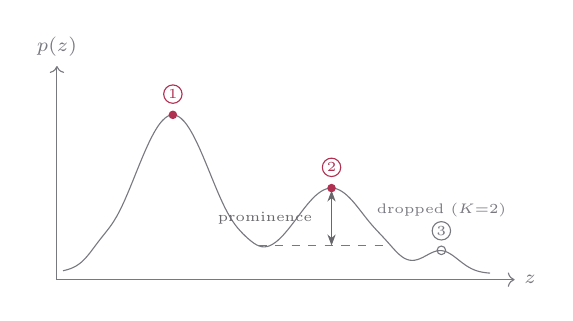
\begin{tikzpicture}[scale=1.55]
        \draw[->,soft] (0,0) -- (3.75,0) node[right,font=\scriptsize]{$z$};
        \draw[->,soft] (0,0) -- (0,1.75) node[above,font=\scriptsize]{$p(z)$};
        \draw[soft,thin,domain=0.05:3.55,samples=160,smooth]
          plot (\x,{1.30*exp(-(\x-0.95)^2/(2*0.10)) + 0.70*exp(-(\x-2.25)^2/(2*0.09))
                    + 0.18*exp(-(\x-3.15)^2/(2*0.02)) + 0.06*exp(-(\x-0.35)^2/(2*0.008))
                    + 0.04*exp(-(\x-1.55)^2/(2*0.008)) + 0.04*exp(-(\x-2.70)^2/(2*0.008)) + 0.05});
        \draw[soft,dashed,thin] (1.65,0.28) -- (2.72,0.28);
        \draw[{Stealth[length=1.4mm]}-{Stealth[length=1.4mm]},ink!70,thin] (2.25,0.28) -- (2.25,0.73);
        \node[font=\tiny,text=ink!70,anchor=east] at (2.17,0.50) {prominence};
        \fill[accent] (0.95,1.35) circle (1.0pt);
        \fill[accent] (2.25,0.75) circle (1.0pt);
        \draw[soft]   (3.15,0.24) circle (1.0pt);
        \node[circle,draw=accent,fill=white,inner sep=0.7pt,font=\tiny,text=accent] at (0.95,1.52) {1};
        \node[circle,draw=accent,fill=white,inner sep=0.7pt,font=\tiny,text=accent] at (2.25,0.92) {2};
        \node[circle,draw=soft,fill=white,inner sep=0.7pt,font=\tiny,text=soft] at (3.15,0.40) {3};
        \node[font=\tiny,text=soft] at (3.15,0.57) {dropped ($K{=}2$)};
      \end{tikzpicture}
      \\[2pt]
      {\scriptsize \textcolor{soft}{Raw Capon spectrum}; \textcolor{accent}{peaks ranked by
       prominence, top $K$ kept}.}
    \end{column}
    \begin{column}{0.38\textwidth}
      \centering
      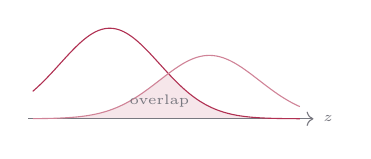
\begin{tikzpicture}[scale=1.15]
        \fill[accent!12]
          plot[domain=0.25:1.548,samples=40,smooth] (\x,{0.7*exp(-(\x-2.0)^2/0.605)})
          -- plot[domain=1.548:2.8,samples=40,smooth] (\x,{1.0*exp(-(\x-0.9)^2/0.605)})
          -- (2.8,0) -- (0.25,0) -- cycle;
        \draw[->,soft] (0,0) -- (3.15,0) node[right,font=\tiny]{$z$};
        \draw[accent,thin,domain=0.05:3.0,samples=60,smooth]
          plot (\x,{1.0*exp(-(\x-0.9)^2/0.605)});
        \draw[accent!60,thin,domain=0.05:3.0,samples=60,smooth]
          plot (\x,{0.7*exp(-(\x-2.0)^2/0.605)});
        \node[font=\tiny,text=soft] at (1.45,0.20) {overlap};
      \end{tikzpicture}
      \\[-1pt]
      {\tiny wide $\sigma$ start: overlapping components, coupled gradients}
      \\[7pt]
      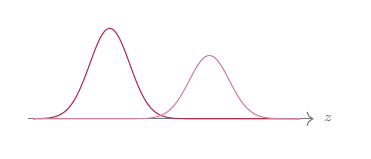
\begin{tikzpicture}[scale=1.15]
        \draw[->,soft] (0,0) -- (3.15,0) node[right,font=\tiny]{$z$};
        \draw[accent,thin,domain=0.05:3.0,samples=60,smooth]
          plot (\x,{1.0*exp(-(\x-0.9)^2/0.097)});
        \draw[accent!60,thin,domain=0.05:3.0,samples=60,smooth]
          plot (\x,{0.7*exp(-(\x-2.0)^2/0.097)});
      \end{tikzpicture}
      \\[-1pt]
      {\tiny small $\sigma_0$ start: disjoint components, easier convergence}
    \end{column}
  \end{columns}
  \vspace{4pt}
  \footnotesize
  \begin{itemize}
    \item Candidate scatterers: local maxima with prominence $\geq 5\%$ of the pixel
          maximum, separated by at least the initial width $\sigma_0$.
    \item Ranked by prominence, top $K$ kept --- $\mu_k$, $a_k$ read directly at the
          surviving peaks; every component starts at the shared width guess
          $\sigma_0 = \max(2\,\Delta\xi,\ \mathrm{span}/8K)$, with $\Delta\xi$ the
          elevation grid step and $\mathrm{span} = \xi_N - \xi_1$ the full grid
          extent ($100$\,m here): an eighth of a component's even share of the
          axis, floored at two grid bins --- deliberately small, so components
          start disjoint and their gradients decouple (right).
    \item Degenerate pixels handled explicitly: fewer than $K$ peaks $\to$ argmax of the
          peak-masked residual; empty profile $\to$ uniform spread over the grid.
  \end{itemize}
\end{frame}

% ---------------------------------------------------------------- 8 Ground truth
\begin{frame}{Ground truth: fitted Gaussian parameters}
  \small
  \begin{columns}[T]
    \begin{column}{0.55\textwidth}
      \begin{minipage}[t][0.68\textheight]{\linewidth}
      \vfill
      Supervised target: the per-pixel array $[a_k,\mu_k,\sigma_k]_{k=1}^{K}$
      ($K{=}2$ today, $K{=}5$ in development), fit to the per-pixel max-normalised
      Capon spectrum $\tilde p = p/p_{\max}$ on the elevation grid $\xi_n$:
      \[
        \mathcal{L} \;=\; \frac{1}{N}\sum_{n=1}^{N}\big(\hat p(\xi_n)-\tilde p(\xi_n)\big)^{2},
        \qquad
        \hat p(\xi) = \sum_{k} a_k\, e^{-\frac{(\xi-\mu_k)^2}{2\sigma_k^2}}
      \]
      \vfill
      One shared loss; each parameter group takes its own projected Adam step:
      \[
        \begin{aligned}
          a_k      &\;\leftarrow\; \big[\, a_k - \eta\,\mathrm{Adam}(\partial_{a_k}\mathcal{L}) \,\big]_{+} \\[-1pt]
          \mu_k    &\;\leftarrow\; \operatorname{clip}_{[\mu^-\!,\;\mu^+]}\big( \mu_k - \eta\,\mathrm{Adam}(\partial_{\mu_k}\mathcal{L}) \big) \\[-1pt]
          \sigma_k &\;\leftarrow\; \operatorname{clip}_{[\sigma^-\!,\;\sigma^+]}\big( \sigma_k - \eta\,\mathrm{Adam}(\partial_{\sigma_k}\mathcal{L}) \big)
        \end{aligned}
      \]
      \vfill
      \end{minipage}
    \end{column}
    \begin{column}{0.43\textwidth}
      \centering
      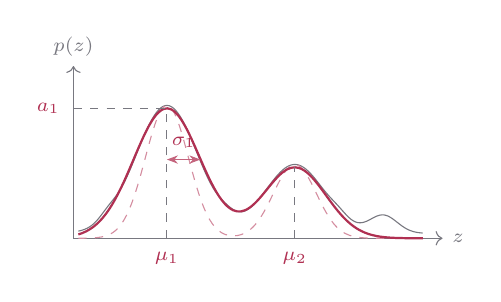
\begin{tikzpicture}[scale=1.25]
        \draw[->,soft] (0,0) -- (3.75,0) node[right,font=\scriptsize]{$z$};
        \draw[->,soft] (0,0) -- (0,1.75) node[above,font=\scriptsize]{$p(z)$};
        \draw[soft,thin,domain=0.05:3.55,samples=160,smooth]
          plot (\x,{1.30*exp(-(\x-0.95)^2/(2*0.10)) + 0.70*exp(-(\x-2.25)^2/(2*0.09))
                    + 0.18*exp(-(\x-3.15)^2/(2*0.02)) + 0.06*exp(-(\x-0.35)^2/(2*0.008))
                    + 0.04*exp(-(\x-1.55)^2/(2*0.008)) + 0.04*exp(-(\x-2.70)^2/(2*0.008)) + 0.05});
        \draw[accent!55,thin,dashed,domain=0.05:3.55,samples=90,smooth]
          plot (\x,{1.35*exp(-(\x-0.95)^2/(2*0.048)) + 0.75*exp(-(\x-2.25)^2/(2*0.048))});
        \draw[accent,thick,domain=0.05:3.55,samples=90,smooth]
          plot (\x,{1.32*exp(-(\x-0.95)^2/(2*0.115)) + 0.72*exp(-(\x-2.25)^2/(2*0.10))});
        \draw[soft,dashed,thin] (0.95,0) -- (0.95,1.32);
        \draw[soft,dashed,thin] (2.25,0) -- (2.25,0.72);
        \draw[soft,dashed,thin] (0,1.32) -- (0.95,1.32);
        \draw[{Stealth[length=1.4mm]}-{Stealth[length=1.4mm]},accent!75,thin]
          (0.95,0.80) -- (1.29,0.80);
        \node[font=\scriptsize,accent,anchor=north] at (0.95,-0.04) {$\mu_1$};
        \node[font=\scriptsize,accent,anchor=north] at (2.25,-0.04) {$\mu_2$};
        \node[font=\scriptsize,accent,anchor=east]  at (-0.04,1.32) {$a_1$};
        \node[font=\scriptsize,accent,anchor=south] at (1.12,0.82) {$\sigma_1$};
      \end{tikzpicture}
      \\[2pt]
      {\scriptsize Same pixel: \textcolor{soft}{Capon spectrum},
       \textcolor{accent!60}{peak initialisation (dashed)},
       \textcolor{accent}{converged fit}; the fitted $[a_k,\mu_k,\sigma_k]$ are the label.}
      \begin{itemize}
        \item {\footnotesize Fitted in normalised space; the winning amplitudes are
              denormalised back, $a_k \to p_{\max}\, a_k$ ($\mu_k$, $\sigma_k$ already
              live on the physical axis).}
        \item {\footnotesize All pixels batched in one optimisation --- not a per-pixel
              loop (next slide); most pixels activate one or two Gaussians (Act III).}
      \end{itemize}
    \end{column}
  \end{columns}
\end{frame}

% ---------------------------------------------------------------- 8a2 Label distributions
\begin{frame}{What the labels look like: fitted parameter distributions}
  \begin{columns}[T]
    \begin{column}{0.32\textwidth}
      \centering
      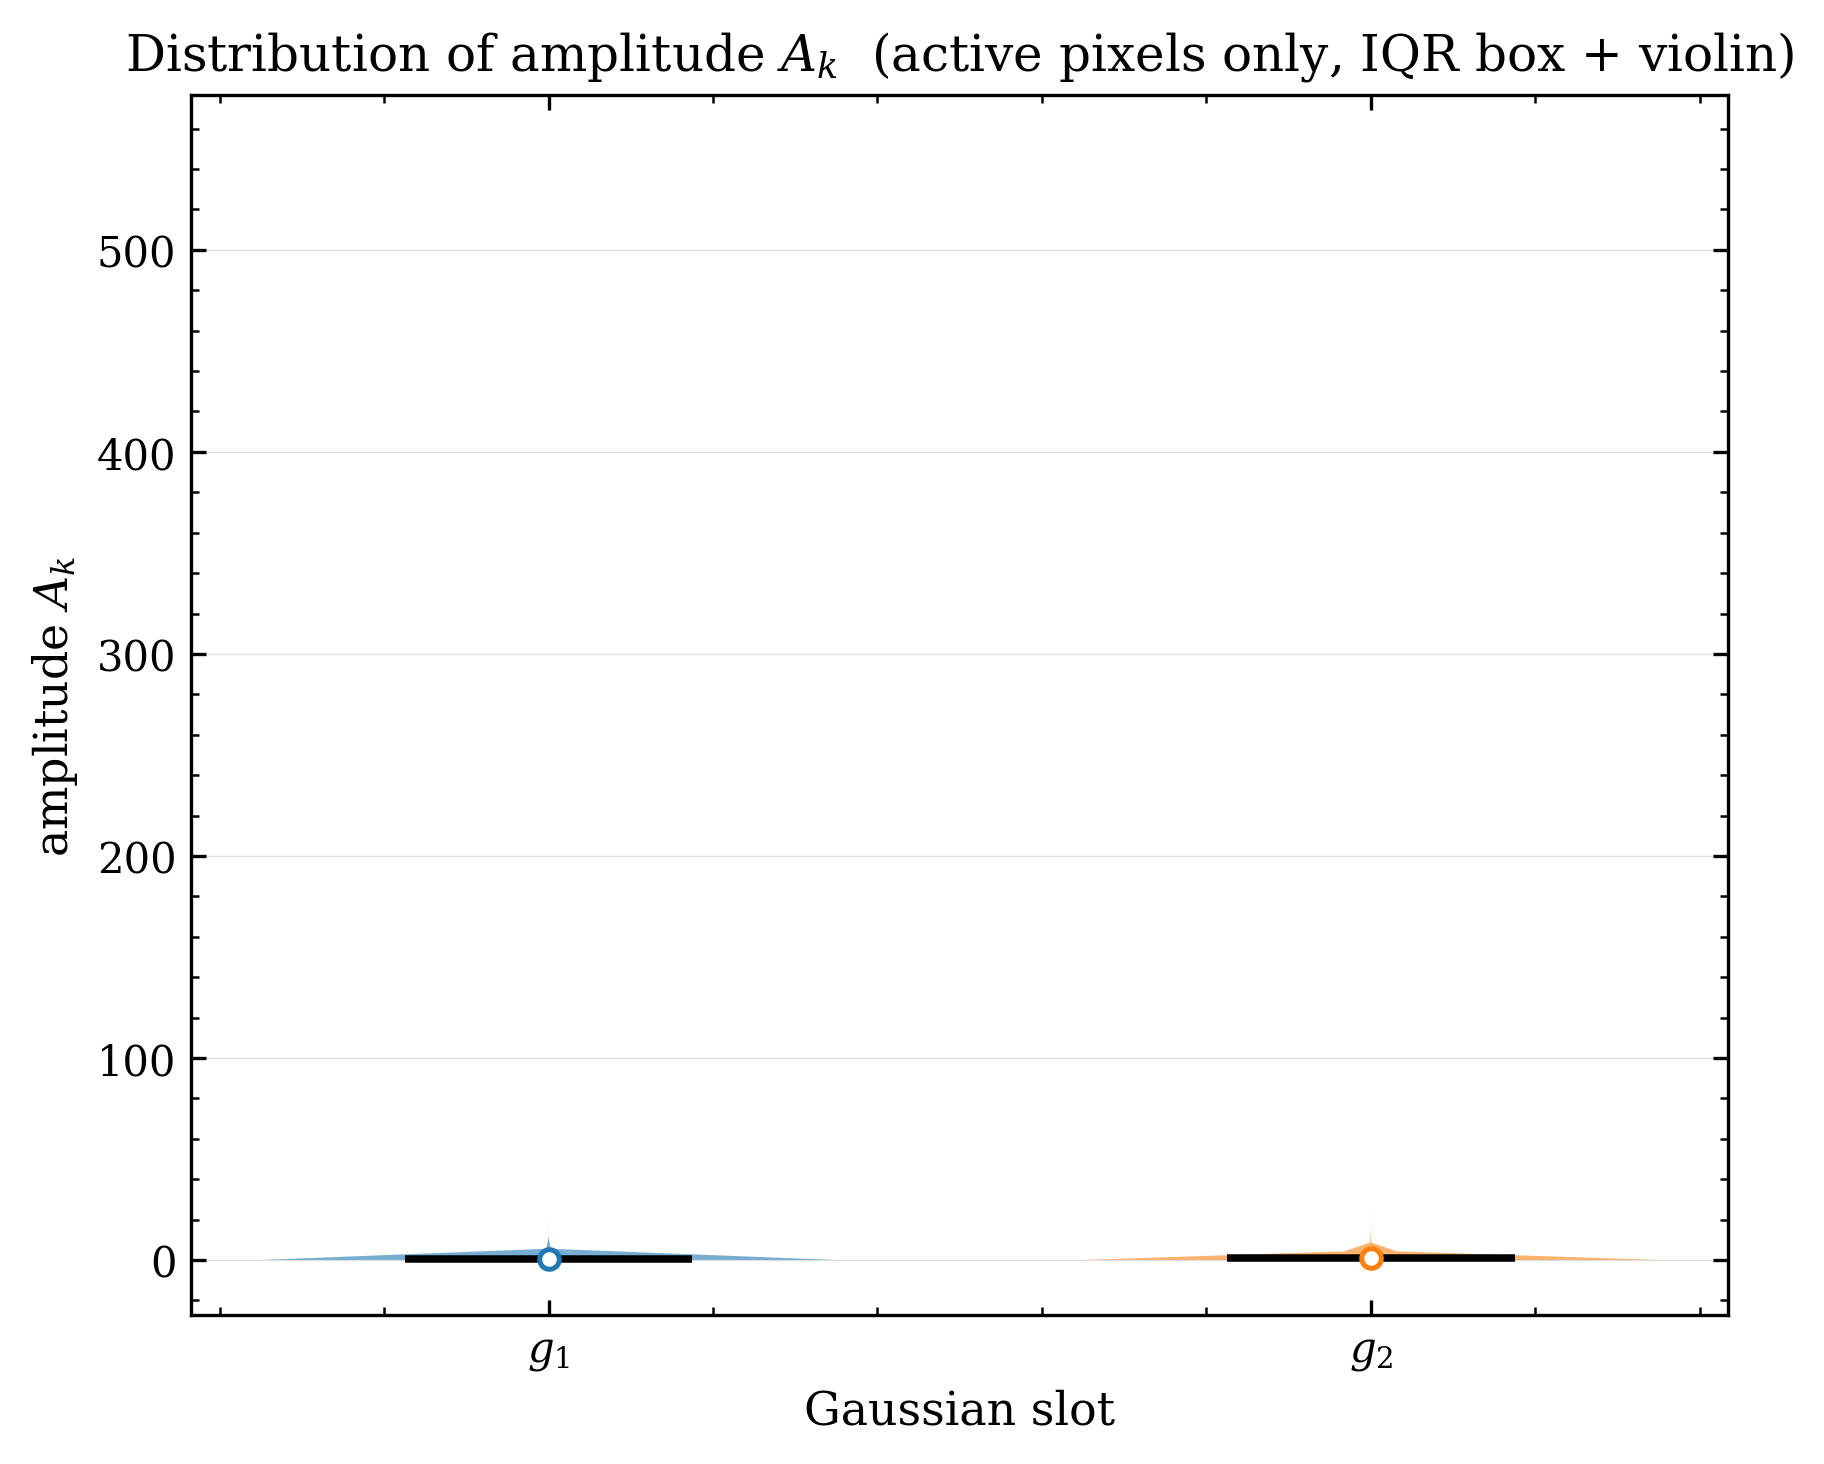
\includegraphics[width=\linewidth]{../figures/param_extraction/label_distributions/amp_distribution.png}
    \end{column}
    \begin{column}{0.32\textwidth}
      \centering
      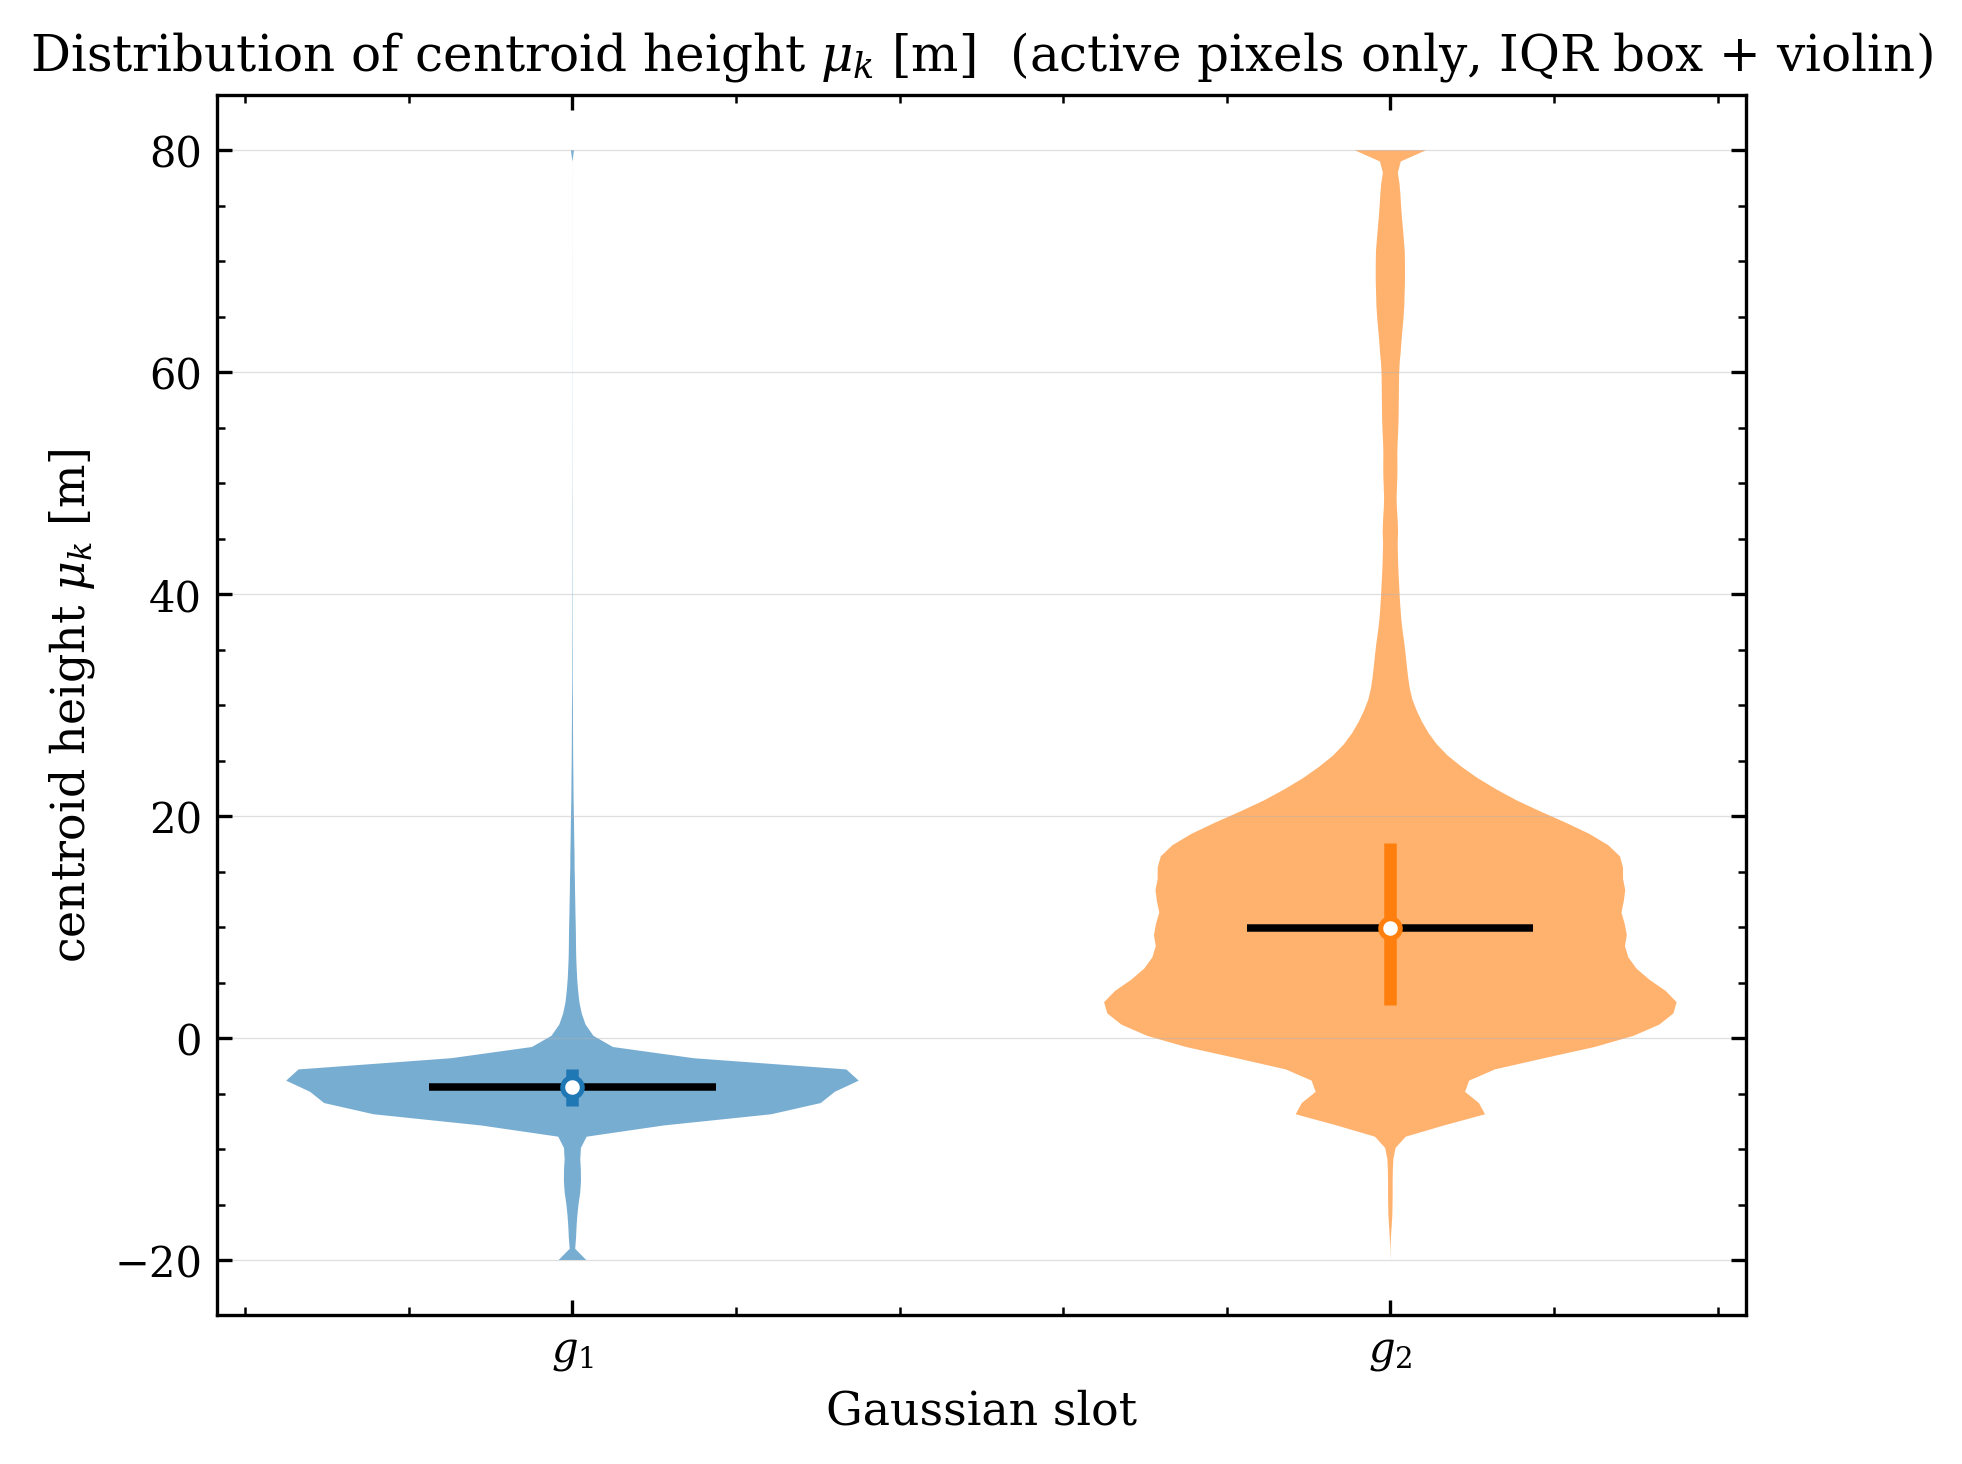
\includegraphics[width=\linewidth]{../figures/param_extraction/label_distributions/mu_distribution.png}
    \end{column}
    \begin{column}{0.32\textwidth}
      \centering
      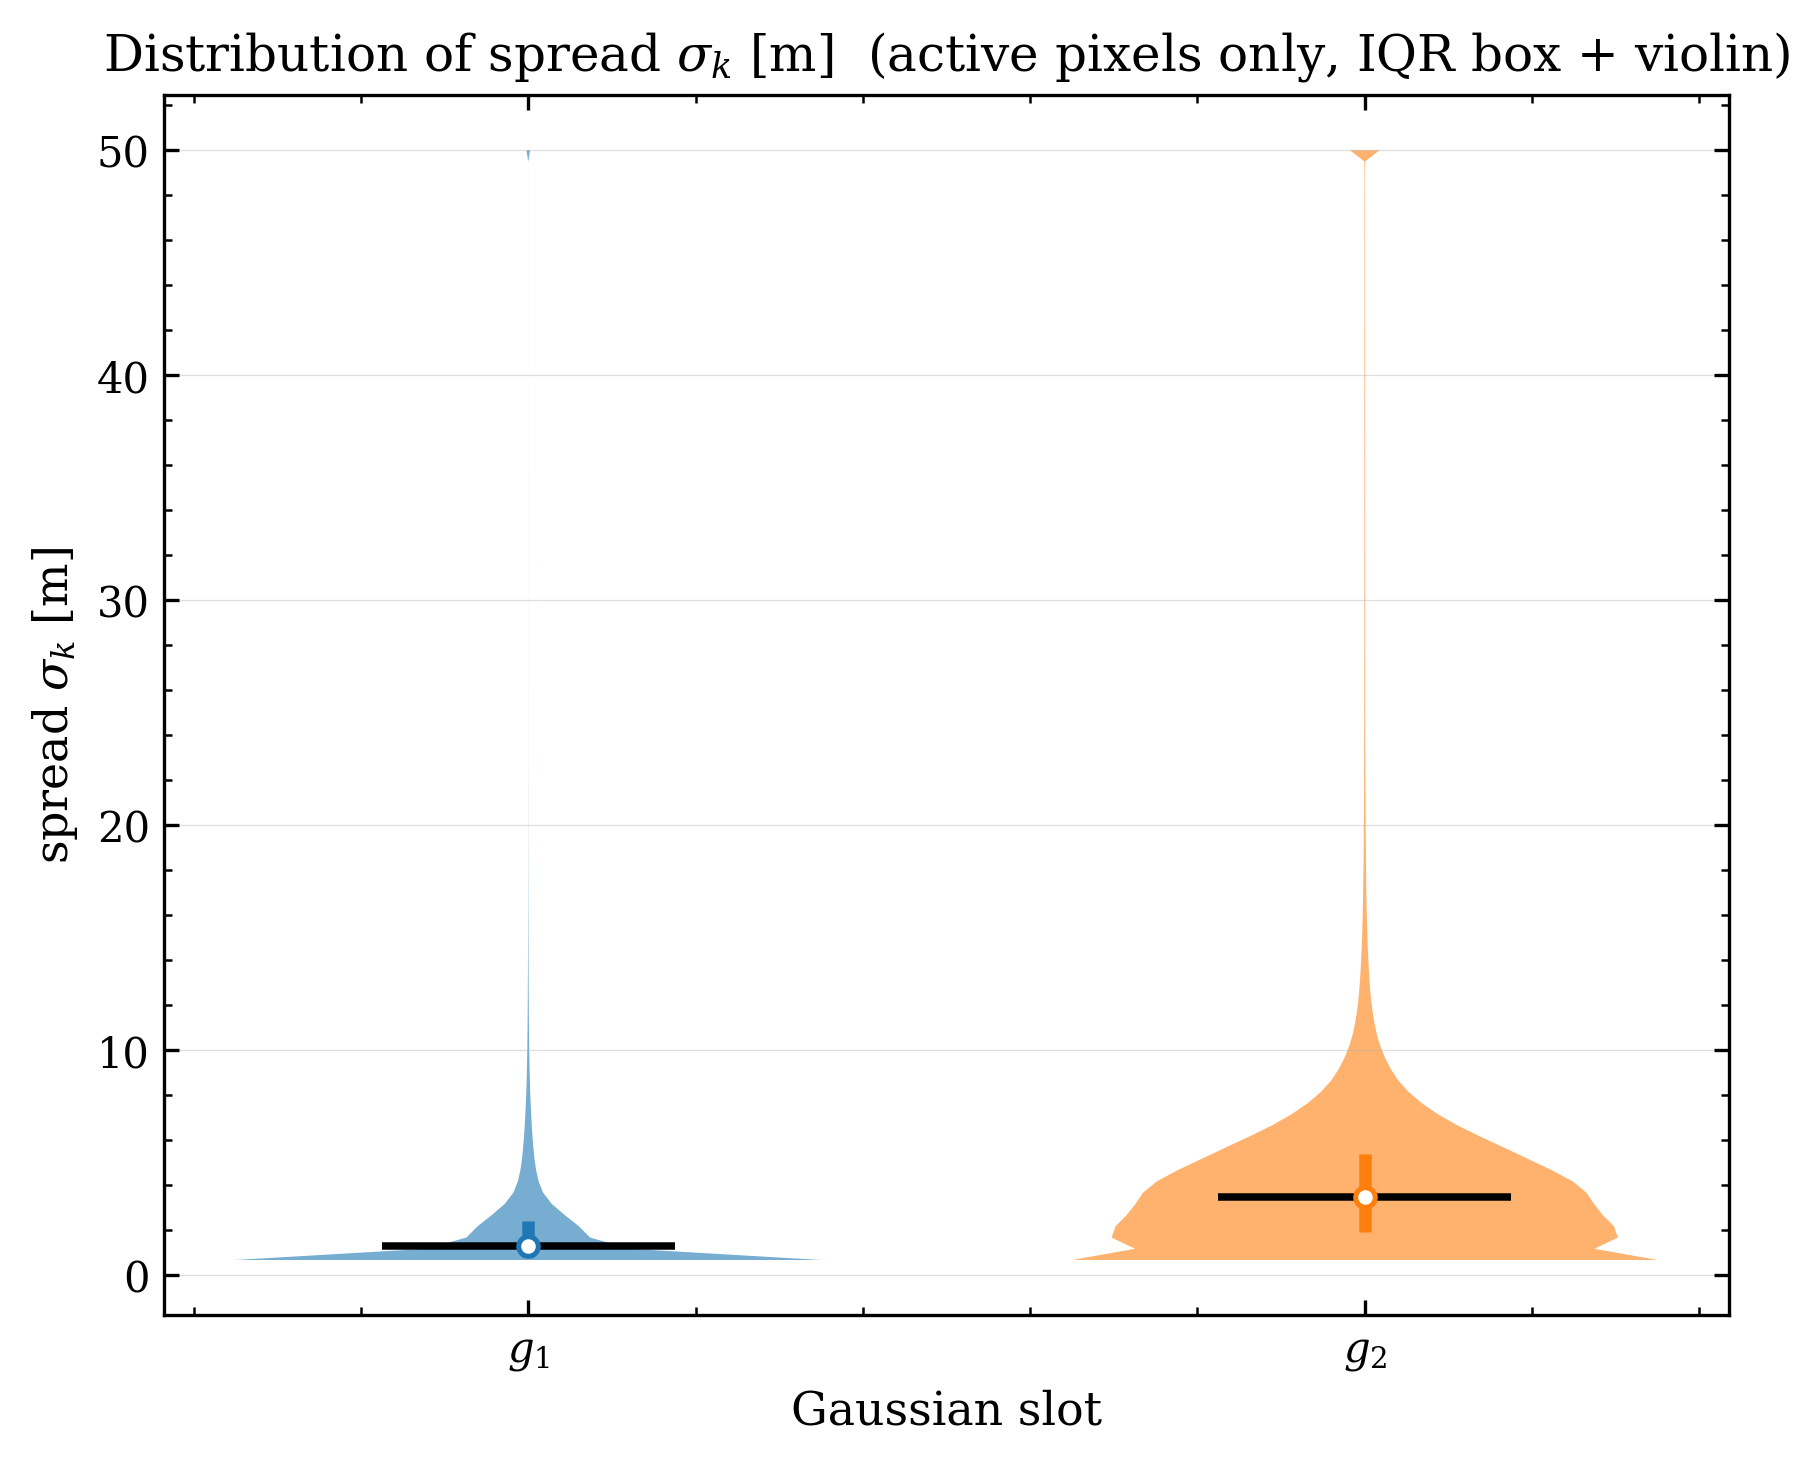
\includegraphics[width=\linewidth]{../figures/param_extraction/label_distributions/sigma_distribution.png}
    \end{column}
  \end{columns}
  \vspace{2pt}
  \small
  \begin{itemize}
    \item Distributions of the supervised targets $[a_k,\mu_k,\sigma_k]$ over \textbf{active pixels only}, split by slot ($g_1$, $g_2$; IQR box $+$ violin).
    \item The second slot $g_2$ sits \textbf{higher} ($\mu_2\!\approx\!10$\,m vs $\mu_1\!\approx\!-5$\,m) and \textbf{broader} ($\sigma_2$ heavier-tailed) --- it takes the elevated, more diffuse scatterer when a pixel activates two.
    \item Amplitudes stay small and tightly peaked; $\mu$ and $\sigma$ carry the long tails the robust scaling (previous act) is built for.
  \end{itemize}
\end{frame}

% ---------------------------------------------------------------- 8b Best-K selection
\begin{frame}{Choosing $K$: fit every order, penalise complexity}
  \begin{columns}[T]
    \begin{column}{0.56\textwidth}
      \footnotesize
      \begin{itemize}
        \item Every active pixel is fitted at \emph{every} order $K = 1,\dots,K_{\max}$,
              all sharing the same peak init (top-$K$ slice).
        \item Per-pixel selection by penalised score
              \[
                S(K) \;=\; \underbrace{\mathrm{MSE}_K}_{\text{fitting component}}
                \;+\; \underbrace{\lambda_K\, K}_{\text{regularization component}}
              \]
              per-$K$ MSE, penalised scores and the best-$K$
              map ride with the dataset as diagnostics.
        \item Today's $K{=}2$ labels run with $\lambda_K = 0$: the fitting component alone
              decides --- the regularization component becomes load-bearing for the $K{=}5$
              extension.
      \end{itemize}
      \vspace{6pt}
      \centering
      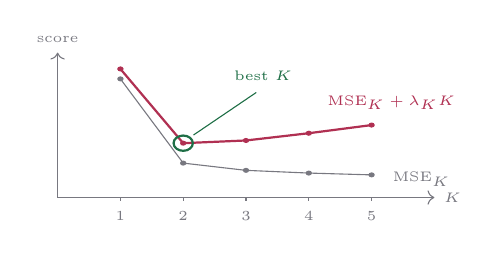
\begin{tikzpicture}[xscale=1.45,yscale=1.15]
        \draw[->,soft] (0,0) -- (3.3,0) node[right,font=\tiny]{$K$};
        \draw[->,soft] (0,0) -- (0,1.6) node[above,font=\tiny]{score};
        \foreach \k in {1,...,5} {
          \draw[soft] (0.55*\k,0) -- (0.55*\k,-0.04);
          \node[font=\tiny,text=soft,anchor=north] at (0.55*\k,-0.05) {\k};
        }
        \draw[soft,thin] (0.55,1.31) -- (1.10,0.38) -- (1.65,0.30) -- (2.20,0.27) -- (2.75,0.25);
        \foreach \p in {(0.55,1.31),(1.10,0.38),(1.65,0.30),(2.20,0.27),(2.75,0.25)}
          \fill[soft] \p circle (0.8pt);
        \draw[accent,thick] (0.55,1.42) -- (1.10,0.60) -- (1.65,0.63) -- (2.20,0.71) -- (2.75,0.80);
        \foreach \p in {(0.55,1.42),(1.10,0.60),(1.65,0.63),(2.20,0.71),(2.75,0.80)}
          \fill[accent] \p circle (0.8pt);
        \draw[good,thick] (1.10,0.60) circle (2.4pt);
        \node[font=\tiny,text=good,anchor=south] at (1.80,1.18) {best $K$};
        \draw[good,thin] (1.74,1.16) -- (1.19,0.69);
        \node[font=\tiny,text=soft,anchor=west] at (2.85,0.20) {$\mathrm{MSE}_K$};
        \node[font=\tiny,text=accent,anchor=south west] at (2.28,0.86) {$\mathrm{MSE}_K + \lambda_K K$};
      \end{tikzpicture}
    \end{column}
    \begin{column}{0.42\textwidth}
      \centering
      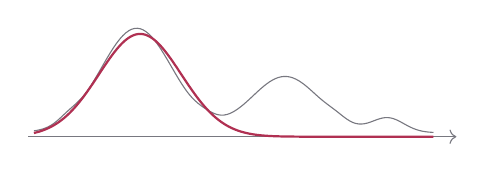
\begin{tikzpicture}[xscale=1.45,yscale=1.02]
        \draw[->,soft] (0,0) -- (3.75,0);
        \draw[soft,thin,domain=0.05:3.55,samples=140,smooth]
          plot (\x,{1.30*exp(-(\x-0.95)^2/(2*0.10)) + 0.70*exp(-(\x-2.25)^2/(2*0.09))
                    + 0.18*exp(-(\x-3.15)^2/(2*0.02)) + 0.06*exp(-(\x-0.35)^2/(2*0.008))
                    + 0.04*exp(-(\x-1.55)^2/(2*0.008)) + 0.04*exp(-(\x-2.70)^2/(2*0.008)) + 0.05});
        \draw[accent,thick,domain=0.05:3.55,samples=80,smooth]
          plot (\x,{1.28*exp(-(\x-0.98)^2/(2*0.13))});
      \end{tikzpicture}
      \\[-1pt]
      {\tiny $K{=}1$: second scatterer missed}
      \\[6pt]
      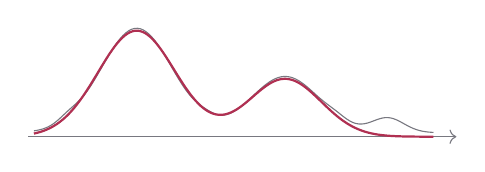
\begin{tikzpicture}[xscale=1.45,yscale=1.02]
        \draw[->,soft] (0,0) -- (3.75,0);
        \draw[soft,thin,domain=0.05:3.55,samples=140,smooth]
          plot (\x,{1.30*exp(-(\x-0.95)^2/(2*0.10)) + 0.70*exp(-(\x-2.25)^2/(2*0.09))
                    + 0.18*exp(-(\x-3.15)^2/(2*0.02)) + 0.06*exp(-(\x-0.35)^2/(2*0.008))
                    + 0.04*exp(-(\x-1.55)^2/(2*0.008)) + 0.04*exp(-(\x-2.70)^2/(2*0.008)) + 0.05});
        \draw[accent,thick,domain=0.05:3.55,samples=80,smooth]
          plot (\x,{1.32*exp(-(\x-0.95)^2/(2*0.115)) + 0.72*exp(-(\x-2.25)^2/(2*0.10))});
      \end{tikzpicture}
      \\[-1pt]
      {\tiny $K{=}2$: both scatterers captured}
      \\[6pt]
      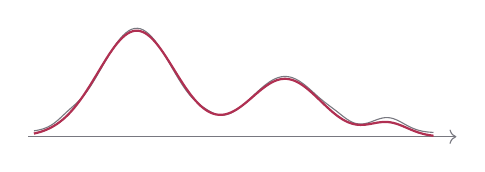
\begin{tikzpicture}[xscale=1.45,yscale=1.02]
        \draw[->,soft] (0,0) -- (3.75,0);
        \draw[soft,thin,domain=0.05:3.55,samples=140,smooth]
          plot (\x,{1.30*exp(-(\x-0.95)^2/(2*0.10)) + 0.70*exp(-(\x-2.25)^2/(2*0.09))
                    + 0.18*exp(-(\x-3.15)^2/(2*0.02)) + 0.06*exp(-(\x-0.35)^2/(2*0.008))
                    + 0.04*exp(-(\x-1.55)^2/(2*0.008)) + 0.04*exp(-(\x-2.70)^2/(2*0.008)) + 0.05});
        \draw[accent,thick,domain=0.05:3.55,samples=80,smooth]
          plot (\x,{1.32*exp(-(\x-0.95)^2/(2*0.115)) + 0.72*exp(-(\x-2.25)^2/(2*0.10))
                    + 0.17*exp(-(\x-3.15)^2/(2*0.03))});
      \end{tikzpicture}
      \\[-1pt]
      {\tiny $K{=}3$: marginal MSE gain}
    \end{column}
  \end{columns}
\end{frame}

% ---------------------------------------------------------------- 8c Best-K map
\begin{frame}{The best-$K$ map: where the second scatterer lives}
  \begin{columns}[c]
    \begin{column}{0.62\textwidth}
      \centering
      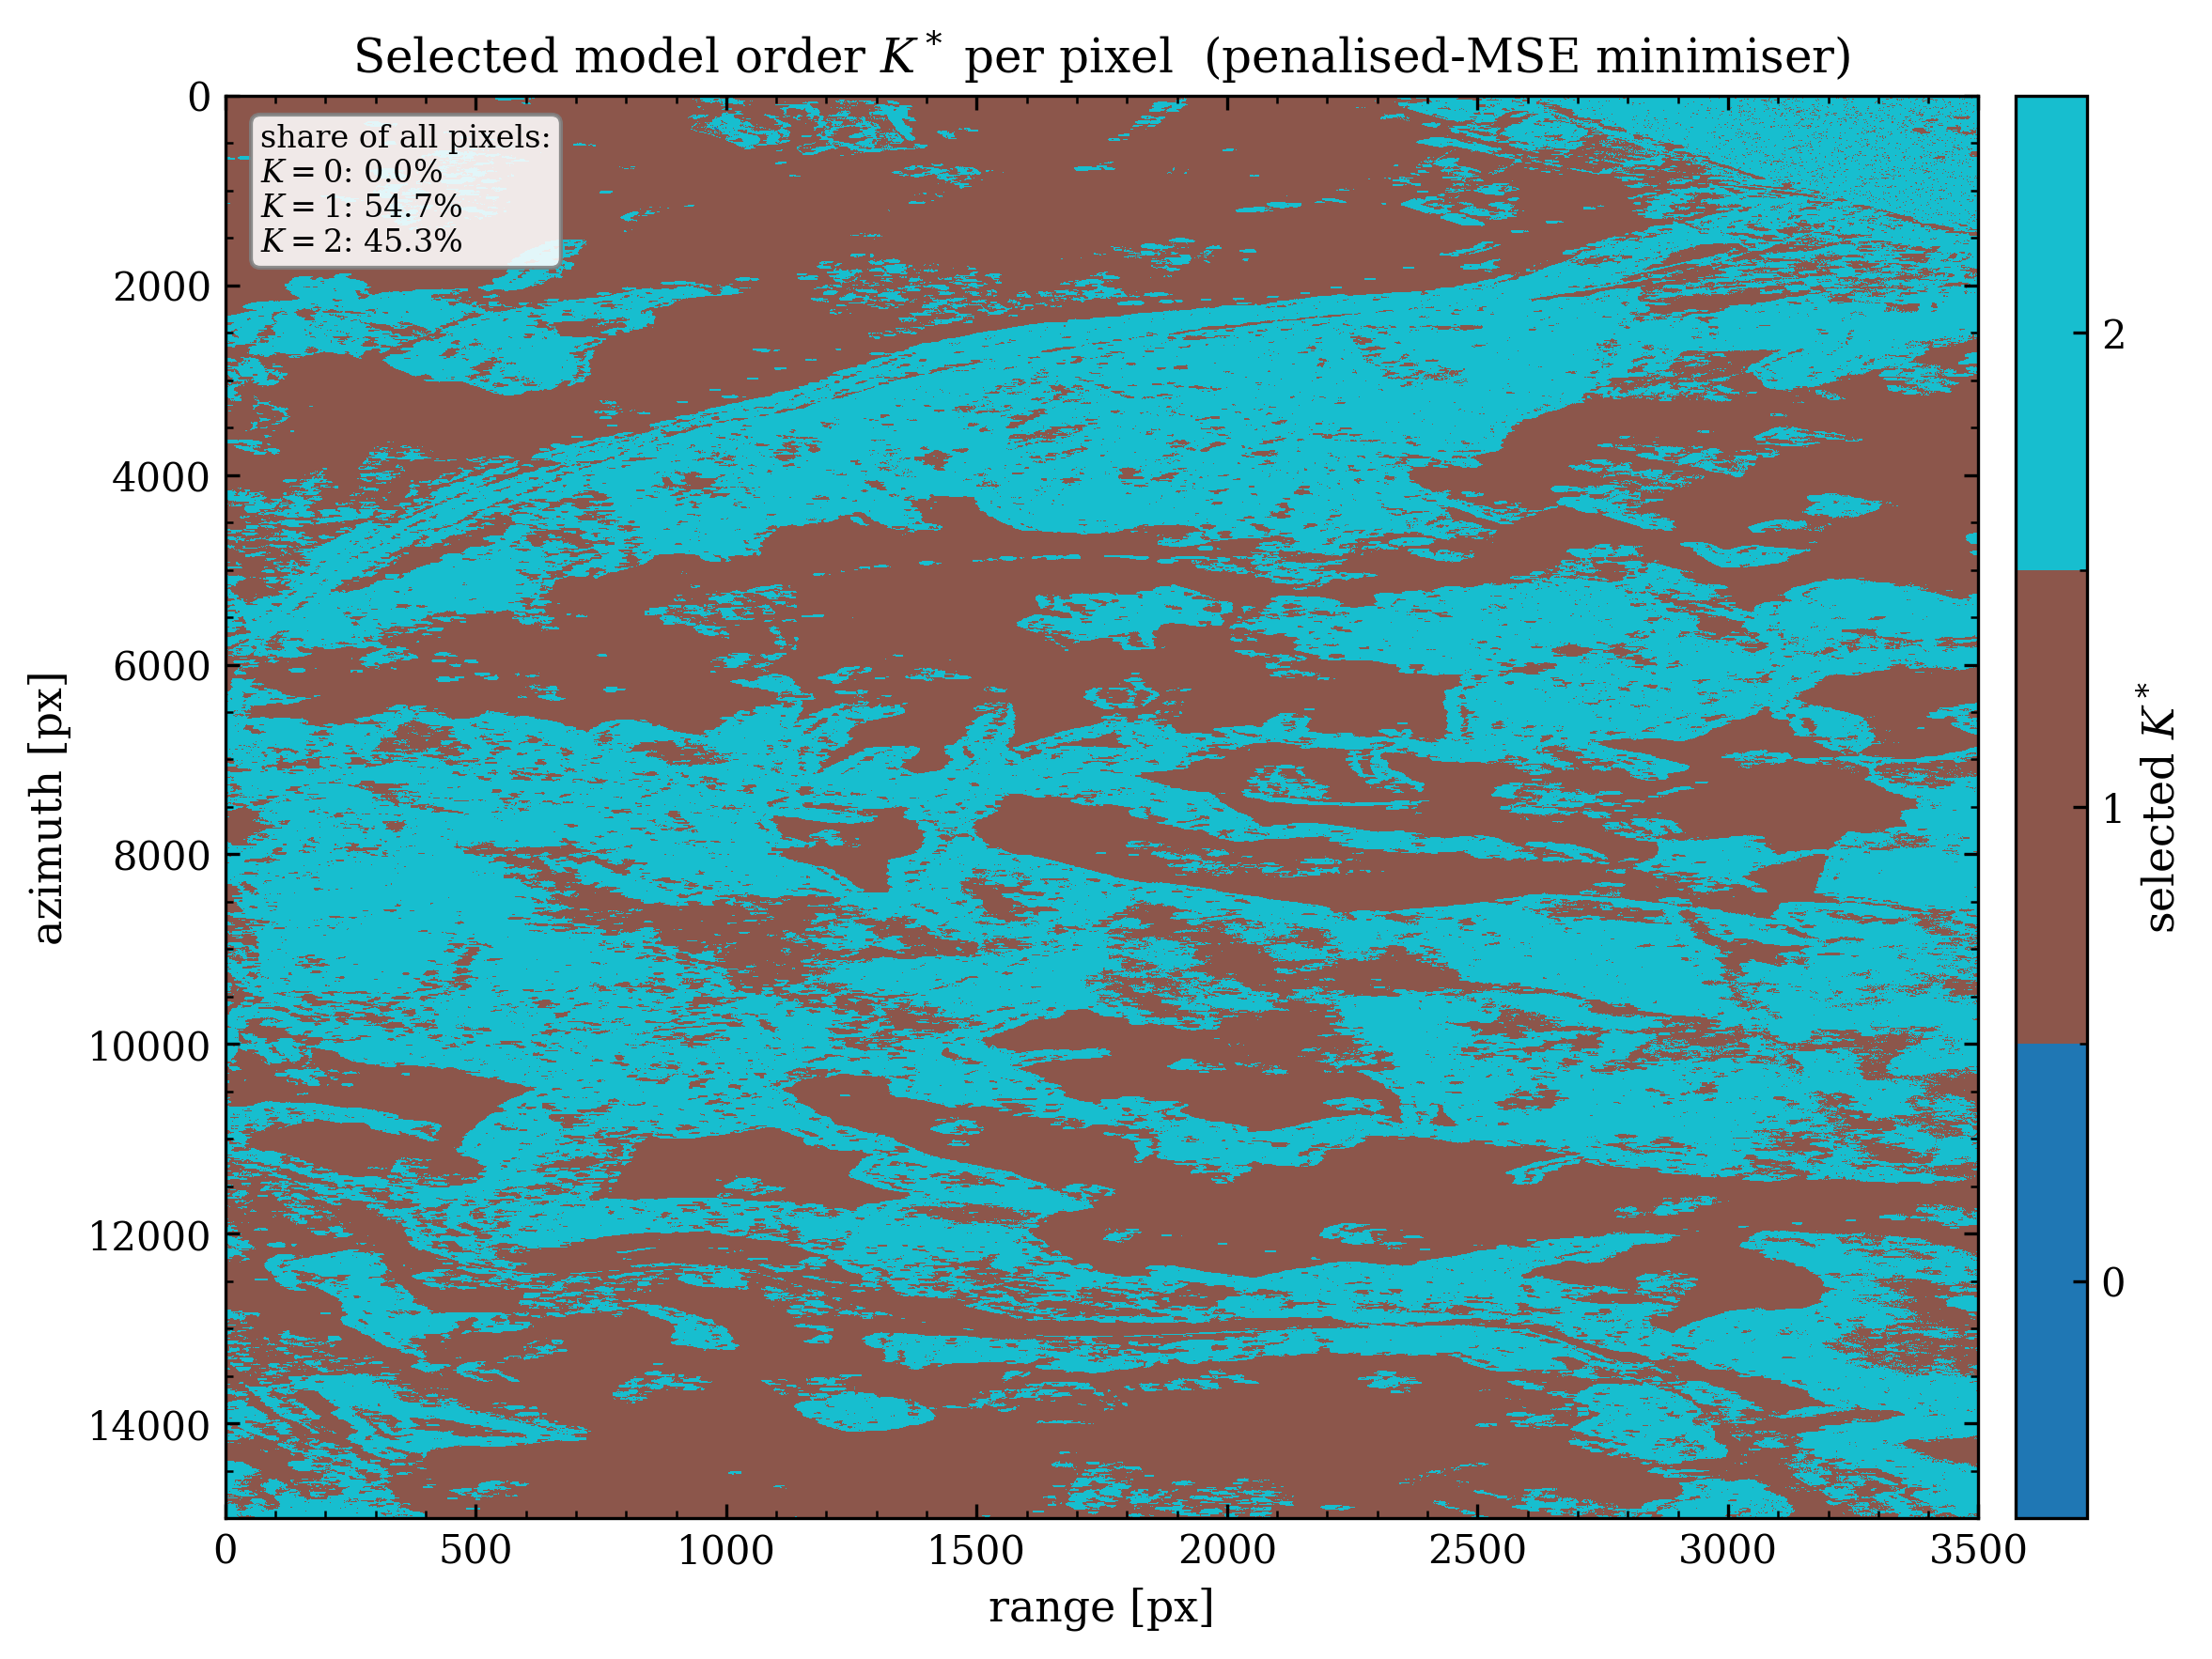
\includegraphics[width=\linewidth,height=0.8\textheight,keepaspectratio]{../figures/param_extraction/best_k_map.png}
    \end{column}
    \begin{column}{0.36\textwidth}
      \small
      \begin{itemize}
        \item The penalised-MSE selection of the previous slide, run per pixel over the full scene.
        \item \textbf{$K{=}1$: 54.7\%}, \textbf{$K{=}2$: 45.3\%}, $K{=}0$: 0.0\% --- the ``most pixels activate one or two Gaussians'' claim, now measured.
        \item The two orders track \textbf{spatial structure}: contiguous regions of single- vs double-scatterer response, following the scene's layover geometry --- not per-pixel noise.
        \item Rides with the dataset as a diagnostic; the complexity price $\lambda_K$ becomes load-bearing for the $K{=}5$ extension.
      \end{itemize}
    \end{column}
  \end{columns}
\end{frame}

% ---------------------------------------------------------------- 9 GT at scale
\begin{frame}{Label generation at scale: multi-GPU parameter extraction}
  \begin{columns}[c]
    \begin{column}{0.40\textwidth}
      \small
      \begin{itemize}\setlength{\itemsep}{10pt}
        \item The fit reformulated as batched gradient optimisation: vectorised over all
              pixels, sharded across GPUs --- full-scene extraction in $\sim$4 minutes.
        \item Labels stop being precious: sweeps over $K$, regularisation and fit modes are
              routine; datasets are regenerated, never patched.
      \end{itemize}
    \end{column}
    \begin{column}{0.58\textwidth}
      \centering
      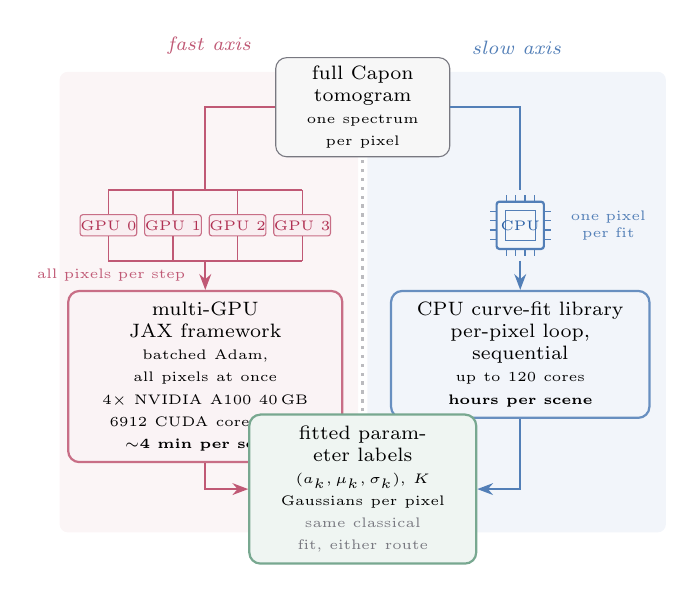
\begin{tikzpicture}
        \node[gate,  text width=20mm] (tomo) at (0,5.4) {full Capon tomogram\\{\tiny one spectrum per pixel}};
        \node[box,   text width=32mm, anchor=north] (gpu) at (-2.0,3.08) {multi-GPU JAX framework\\{\tiny batched Adam, all pixels at once}\\{\tiny 4$\times$ NVIDIA A100 40\,GB}\\{\tiny 6912 CUDA cores each}\\{\tiny \textbf{$\sim$4 min per scene}}};
        \node[box, draw=argA!70, fill=argA!6, text width=30mm, anchor=north] (cpu) at (2.0,3.08) {CPU curve-fit library\\per-pixel loop, sequential\\{\tiny up to 120 cores}\\{\tiny \textbf{hours per scene}}};
        \node[box, draw=good!60, fill=good!7, text width=26mm] (lab) at (0,0.55) {fitted parameter labels\\{\tiny $(a_k,\mu_k,\sigma_k)$, $K$ Gaussians per pixel}\\{\tiny \textcolor{soft}{same classical fit, either route}}};

        \begin{scope}[shift={(-2.0,3.9)}]
          \foreach \i/\x in {0/-1.23,1/-0.41,2/0.41,3/1.23} {
            \draw[accent!70,thin,fill=accent!8,rounded corners=1pt] (\x-0.36,-0.135) rectangle (\x+0.36,0.135);
            \node[font=\tiny,text=accent] at (\x,0) {GPU \i};
          }
          \draw[accent!80,thick] (-1.23,0.45)  -- (1.23,0.45);
          \draw[accent!80,thick] (-1.23,-0.45) -- (1.23,-0.45);
          \foreach \x in {-1.23,-0.41,0.41,1.23} {
            \draw[accent!80,thin] (\x,0.45)  -- (\x,0.14);
            \draw[accent!80,thin] (\x,-0.14) -- (\x,-0.45);
          }
        \end{scope}
        \node[font=\tiny,text=accent!80,anchor=east] at (-2.13,3.27) {all pixels per step};

        \begin{scope}[shift={(2.0,3.9)}]
          \foreach \p in {-0.18,-0.06,0.06,0.18} {
            \draw[argA!80,thin] (\p,0.30)  -- (\p,0.39);
            \draw[argA!80,thin] (\p,-0.30) -- (\p,-0.39);
            \draw[argA!80,thin] (0.30,\p)  -- (0.39,\p);
            \draw[argA!80,thin] (-0.30,\p) -- (-0.39,\p);
          }
          \draw[argA!80,thick,fill=argA!5,rounded corners=1pt] (-0.30,-0.30) rectangle (0.30,0.30);
          \draw[argA!80,thin] (-0.19,-0.19) rectangle (0.19,0.19);
          \node[font=\tiny,text=argA] at (0,0) {CPU};
        \end{scope}
        \node[font=\tiny,text=argA!80,align=center,anchor=west] at (2.52,3.9) {one pixel\\per fit};

        \begin{scope}[on background layer]
          \fill[accent!5,rounded corners=3pt] (-3.85,0.0) rectangle (-0.06,5.85);
          \fill[argA!6,rounded corners=3pt]   (0.06,0.0)  rectangle (3.85,5.85);
          \draw[soft!50,dotted,very thick] (0,-0.15) -- (0,6.0);
        \end{scope}
        \node[font=\scriptsize\itshape,text=accent!80,anchor=south] at (-1.95,5.95) {fast axis};
        \node[font=\scriptsize\itshape,text=argA!80,anchor=south]   at (1.95,5.95)  {slow axis};

        \draw[accent!80,thick] (tomo.west) -| (-2.0,4.35);
        \draw[flow] (-2.0,3.45) -- (gpu.north);
        \draw[flow] (gpu.south) |- (lab.west);
        \draw[argA!80,thick] (tomo.east) -| (2.0,4.35);
        \draw[flow, argA!80] (2.0,3.45) -- (cpu.north);
        \draw[flow, argA!80] (cpu.south) |- (lab.east);
      \end{tikzpicture}
    \end{column}
  \end{columns}
\end{frame}

% ---------------------------------------------------------------- 10 Input/output
\begin{frame}{Input and output representation}
  \centering
  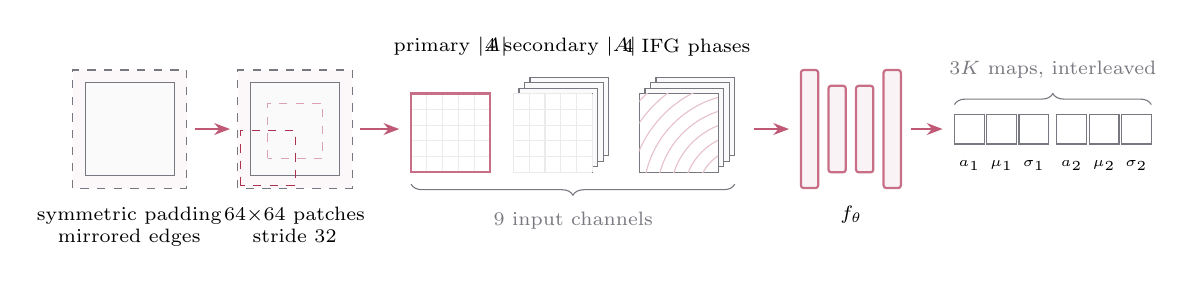
\begin{tikzpicture}
    \draw[soft,dashed,thin,fill=accent!4] (0,0.3) rectangle (1.45,1.8);
    \draw[soft,thin,fill=black!2] (0.16,0.46) rectangle (1.29,1.64);
    \node[font=\scriptsize,align=center,anchor=north] at (0.72,0.18) {symmetric padding\\mirrored edges};
    \draw[flow] (1.55,1.05) -- (2.0,1.05);
    \draw[soft,dashed,thin,fill=accent!4] (2.1,0.3) rectangle (3.55,1.8);
    \draw[soft,thin,fill=black!2] (2.26,0.46) rectangle (3.39,1.64);
    \draw[accent,dashed,thin] (2.13,0.33) rectangle ++(0.7,0.7);
    \draw[accent!45,dashed,thin] (2.48,0.68) rectangle ++(0.7,0.7);
    \node[font=\scriptsize,align=center,anchor=north] at (2.82,0.18) {$64{\times}64$ patches\\stride 32};
    \draw[flow] (3.65,1.05) -- (4.15,1.05);
    \draw[soft,thin,fill=white] (4.3,0.5) rectangle ++(1.0,1.0);
    \draw[black!8,step=0.2,shift={(4.3,0.5)}] (0,0) grid (1.0,1.0);
    \draw[accent!70,thick] (4.3,0.5) rectangle ++(1.0,1.0);
    \node[font=\scriptsize,anchor=south] at (4.8,1.85) {primary $|A|$};
    \foreach \i in {3,2,1} \draw[soft,thin,fill=black!2] (5.6+0.07*\i,0.5+0.07*\i) rectangle ++(1.0,1.0);
    \draw[soft,thin,fill=white] (5.6,0.5) rectangle ++(1.0,1.0);
    \draw[black!8,step=0.2,shift={(5.6,0.5)}] (0,0) grid (1.0,1.0);
    \node[font=\scriptsize,anchor=south] at (6.2,1.85) {4 secondary $|A|$};
    \foreach \i in {3,2,1} \draw[soft,thin,fill=black!2] (7.2+0.07*\i,0.5+0.07*\i) rectangle ++(1.0,1.0);
    \draw[soft,thin,fill=white] (7.2,0.5) rectangle ++(1.0,1.0);
    \begin{scope} \clip (7.2,0.5) rectangle ++(1.0,1.0); \foreach \r in {0.45,0.62,...,1.85} \draw[accent!30,thin] (8.55,0.2) circle (\r); \end{scope}
    \node[font=\scriptsize,anchor=south] at (7.8,1.85) {4 IFG phases};
    \draw[decorate,decoration={brace,amplitude=4pt,mirror},soft] (4.3,0.35) -- (8.41,0.35);
    \node[font=\scriptsize,text=soft,anchor=north] at (6.36,0.12) {9 input channels};
    \draw[flow] (8.65,1.05) -- (9.1,1.05);
    \foreach \x/\h in {9.25/1.5,9.6/1.1,9.95/1.1,10.3/1.5} \draw[accent!70,thick,fill=accent!6,rounded corners=1pt] (\x,1.05-\h/2) rectangle ++(0.22,\h);
    \node[font=\scriptsize,anchor=north] at (9.89,0.2) {$f_\theta$};
    \draw[flow] (10.65,1.05) -- (11.05,1.05);
    \foreach \x/\lbl in {11.2/{$a_1$},11.61/{$\mu_1$},12.02/{$\sigma_1$},12.5/{$a_2$},12.91/{$\mu_2$},13.32/{$\sigma_2$}} { \draw[soft,thin,fill=white] (\x,0.86) rectangle ++(0.38,0.38); \node[font=\tiny,anchor=north] at (\x+0.19,0.78) {\lbl}; }
    \draw[decorate,decoration={brace,amplitude=4pt},soft] (11.2,1.36) -- (13.7,1.36);
    \node[font=\scriptsize,text=soft,anchor=south] at (12.45,1.57) {$3K$ maps, interleaved};
  \end{tikzpicture}
  \\[10pt]
  \small
  \begin{itemize}
    \item Scenes are symmetrically padded (edge-mirrored) so the $64\times 64$, stride-32
          patch grid tiles them exactly; sliding-window stitching undoes the overlap at inference.
    \item The $3K$ output channels are interleaved per scatterer ---
          $a_1,\mu_1,\sigma_1,a_2,\mu_2,\sigma_2,\dots$ --- not grouped by parameter type.
    \item Outputs live in normalized space; denormalised and clamped to physical bounds
          before any curve is reconstructed.
    \item Current configuration $K{=}2$ (6 maps); the $K{=}5$ variant (15 maps) in development.
  \end{itemize}
\end{frame}

% ---------------------------------------------------------------- 10b Real channel distributions
\begin{frame}{Two input channels, two regimes}
  \begin{columns}[T]
    \begin{column}{0.5\textwidth}
      \centering
      {\small\textbf{\textcolor{accent}{primary amplitude}}}\\[3pt]
      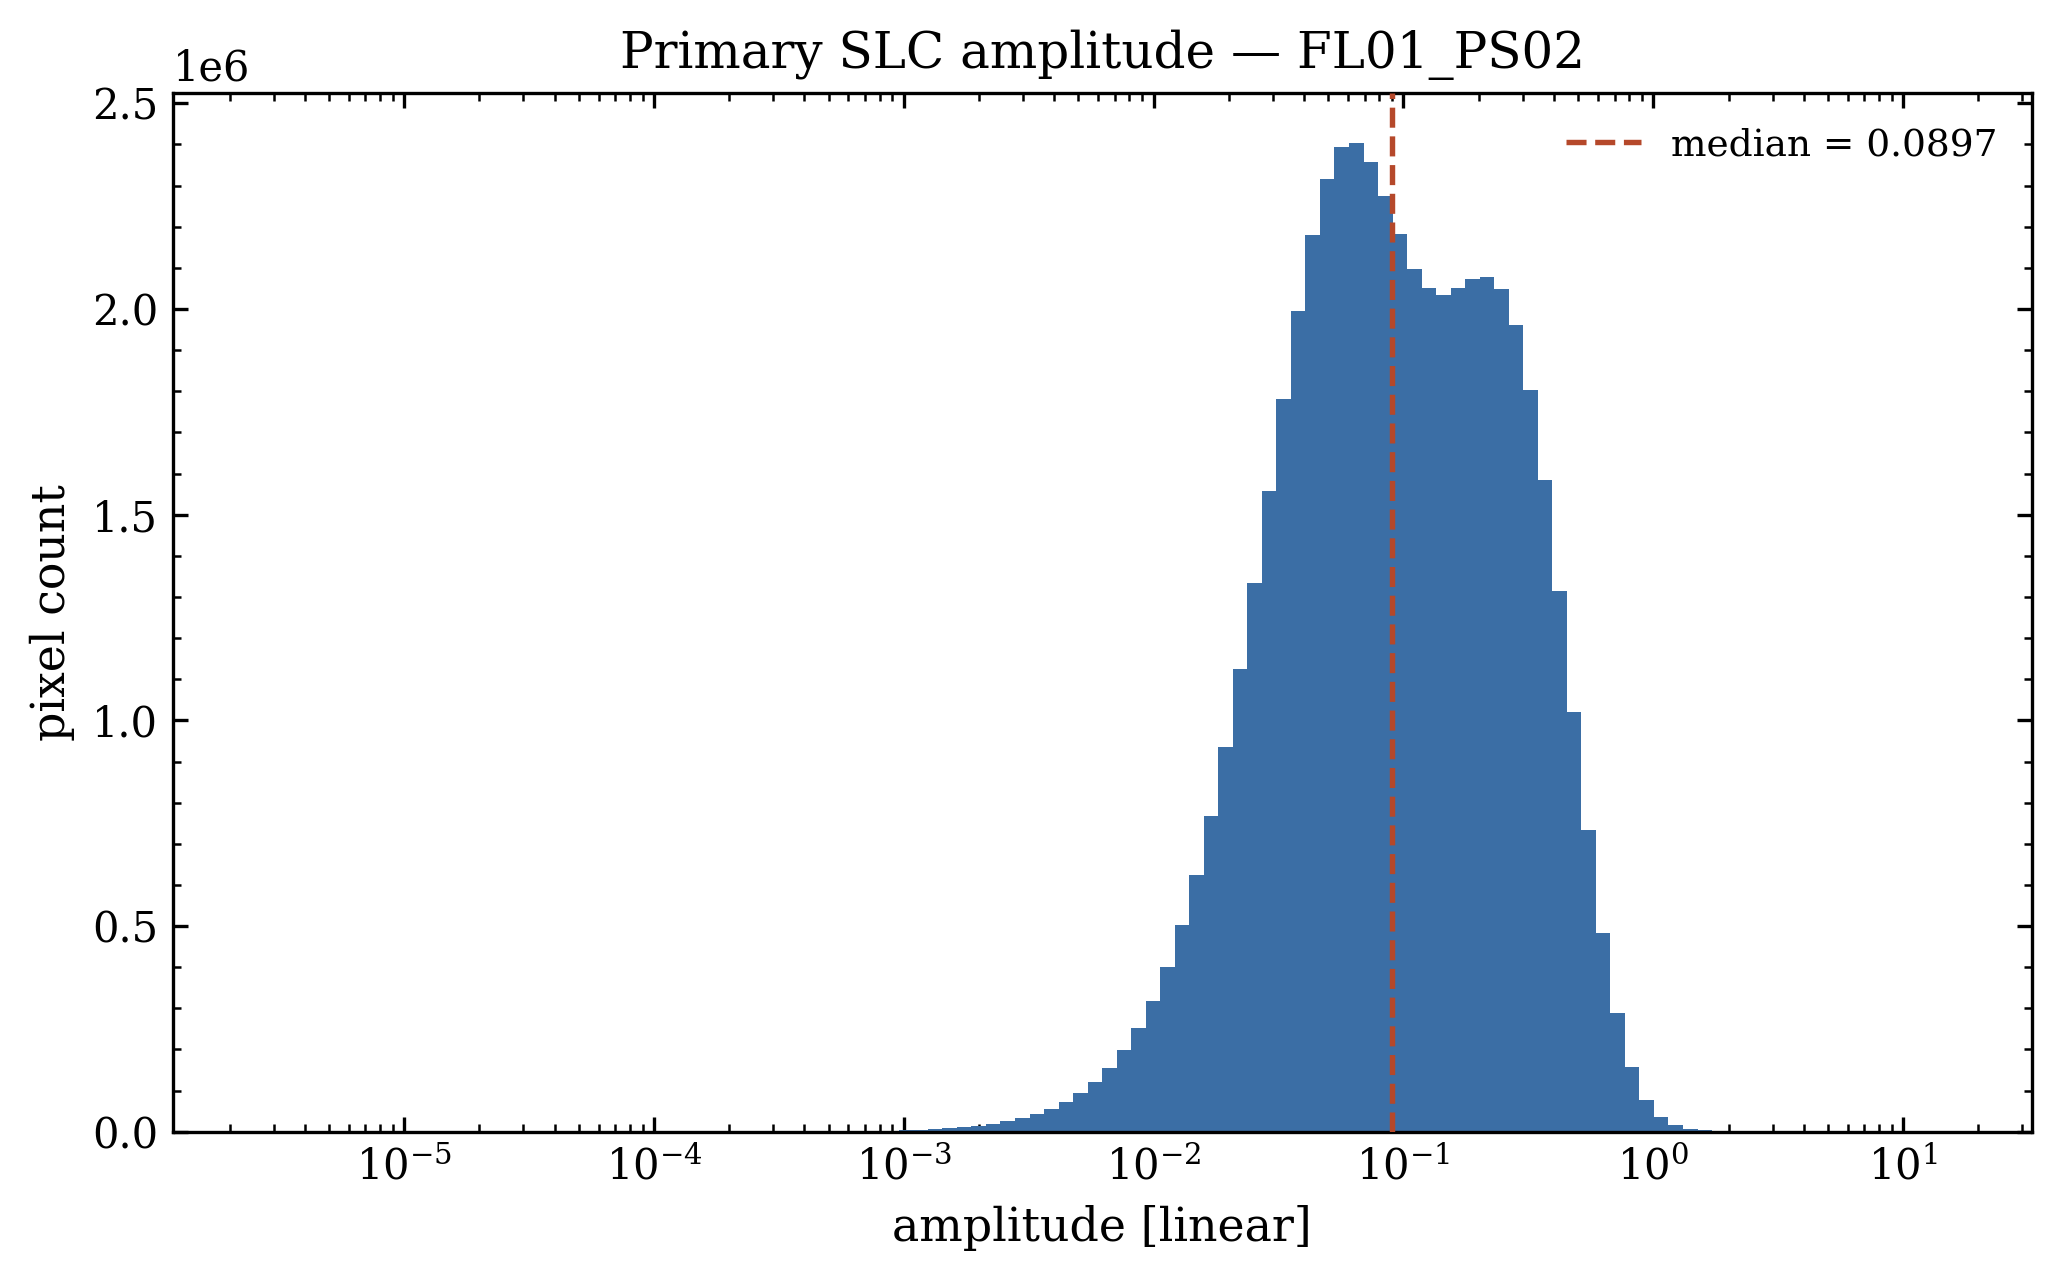
\includegraphics[width=\linewidth]{../figures/preprocessing_inference/channel_distributions/pass_00_FL01_PS02_amplitude.png}\\[3pt]
      {\scriptsize\color{soft} Log-scaled axis: the bulk sits near $10^{-1}$ but the tail runs past $10^{0}$ --- orders of magnitude in one channel. \textcolor{accent}{Heavy-tailed} $\rightarrow$ robust log1p scaling.}
    \end{column}
    \begin{column}{0.5\textwidth}
      \centering
      {\small\textbf{\textcolor{good}{interferogram phase}}}\\[3pt]
      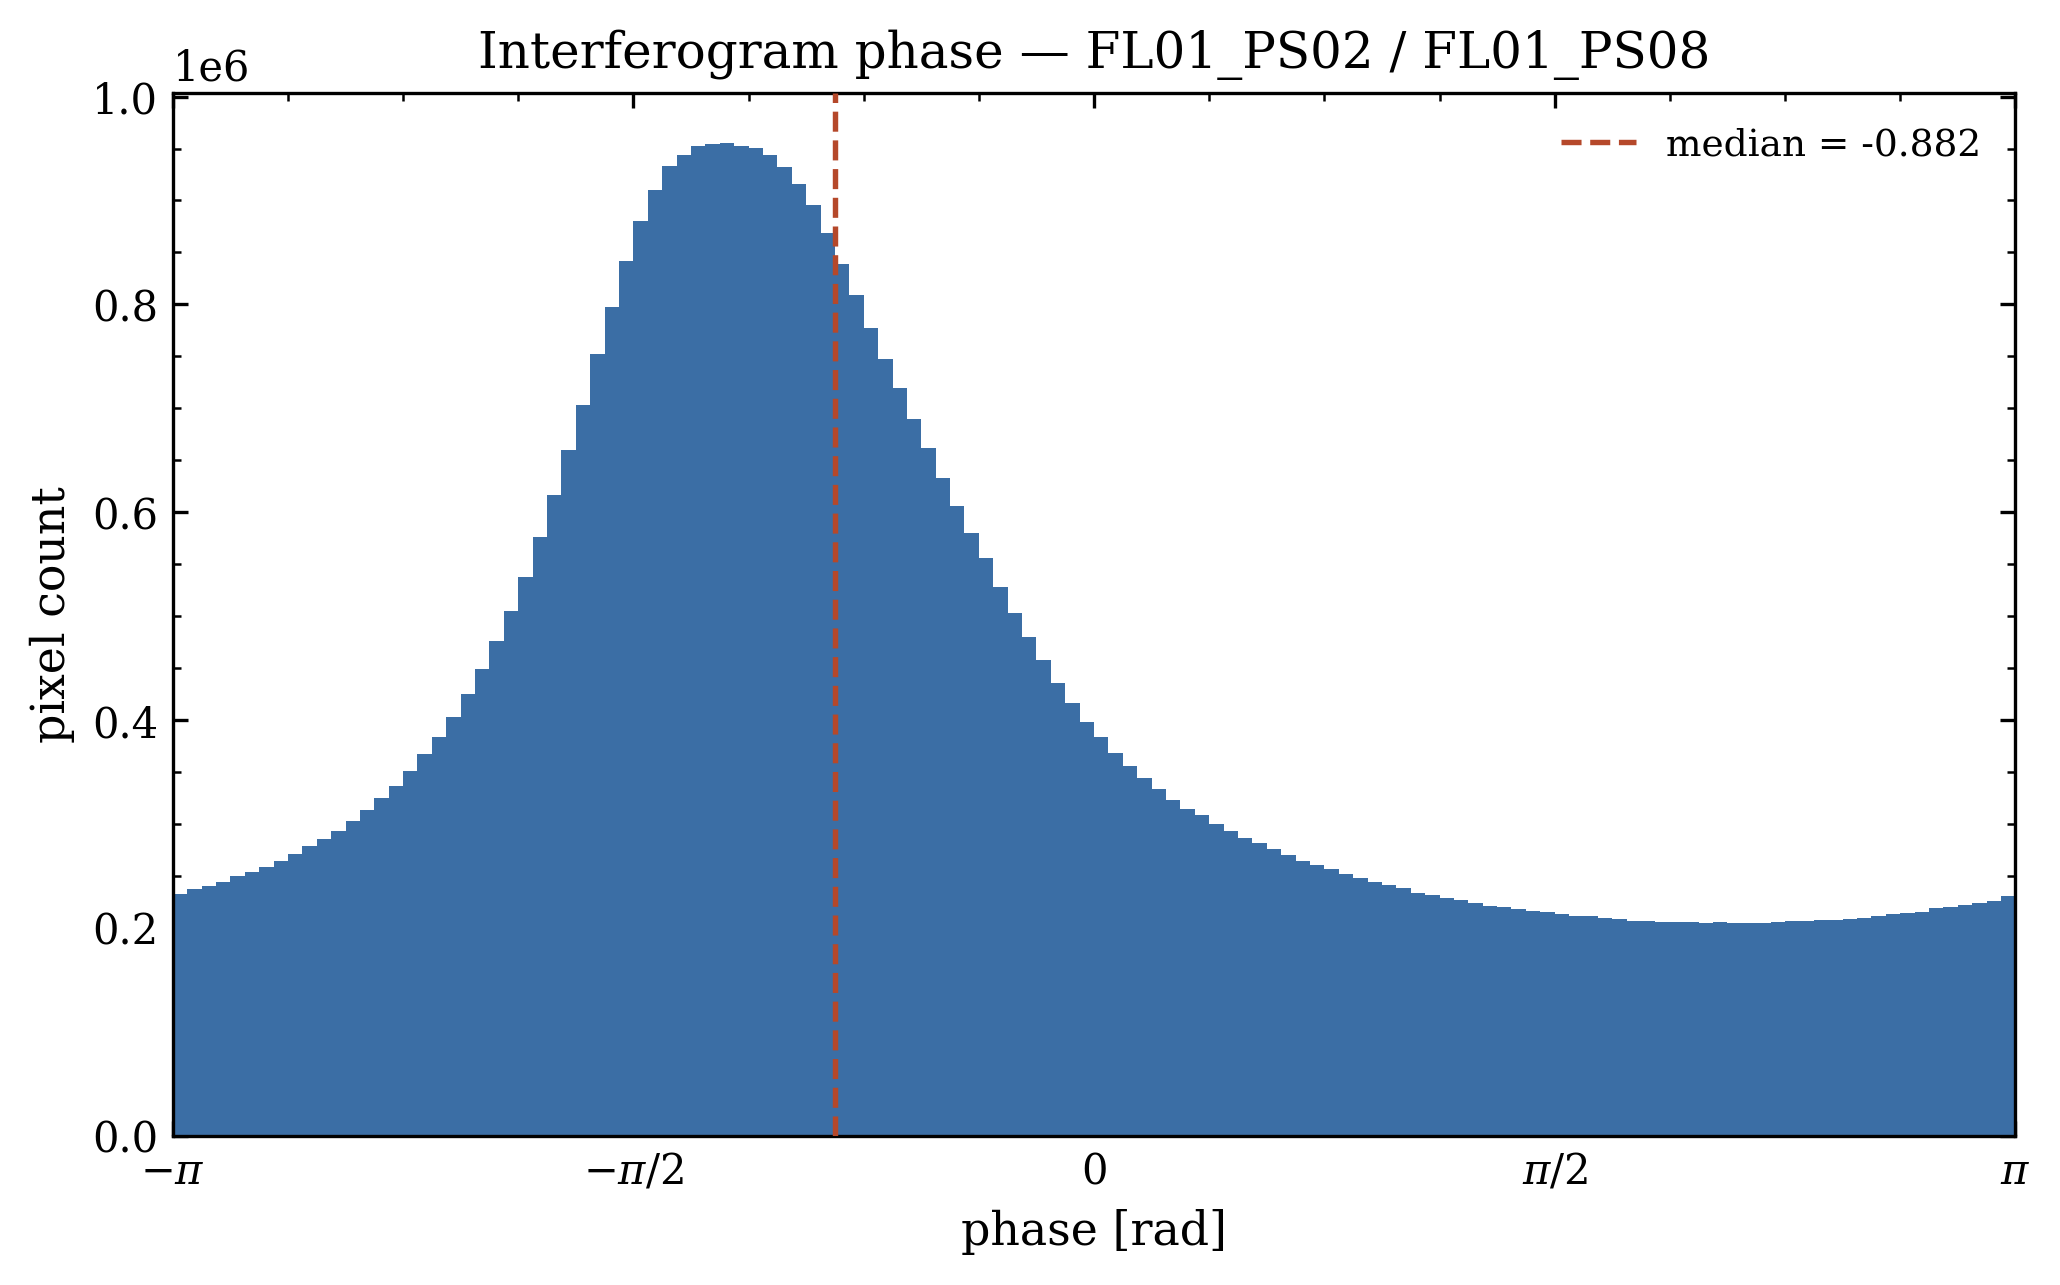
\includegraphics[width=\linewidth]{../figures/preprocessing_inference/channel_distributions/interferogram_03_FL01_PS08_phase.png}\\[3pt]
      {\scriptsize\color{soft} Confined to $[-\pi,\pi]$ by construction, a single broad mode --- no tail to tame. \textcolor{good}{Bounded by physics} $\rightarrow$ fixed $\div\,\pi$.}
    \end{column}
  \end{columns}
  \vspace{5pt}
  \centering
  {\footnotesize Real F-SAR channels (primary PS02, IFG PS02/PS08). The nine inputs split cleanly into these two shapes --- and the normalization strategy (next) follows the split.}
\end{frame}

% ---------------------------------------------------------------- 12 Strategy table
\begin{frame}{Per-channel normalization --- old $\to$ new, channel by channel}
  \begin{columns}[c]
    \begin{column}{0.58\textwidth}
      \centering
      \scriptsize
      \renewcommand{\arraystretch}{1.75}
      \setlength{\tabcolsep}{3pt}
      {\color{soft} z-score --- standard score \quad$\cdot$\quad IQR --- interquartile range}\\[5pt]
      \begin{tabular}{@{}l l c l l@{}}
        \toprule
        channel & old & & new & why \\
        \midrule
        pass / mag     & \textcolor{soft}{z-score (log1p)}        & $\to$ & \textbf{\textcolor{accent}{robust IQR (log1p)}} & tail sets $\mu$, $\sigma$ \\
        ifg / phase    & \textcolor{soft}{min--max ($p_{99.9}$)}  & $\to$ & \textbf{\textcolor{good}{fixed $\div\,\pi$}}    & bounded by physics \\
        \addlinespace
        out / $a$      & \textcolor{soft}{z-score}                & $\to$ & \textbf{\textcolor{accent}{robust IQR (log1p)}} & heavy-tailed target \\
        out / $\sigma$ & \textcolor{soft}{z-score}                & $\to$ & \textbf{\textcolor{accent}{robust IQR (log1p)}} & heavy-tailed target \\
        out / $\mu$    & \textcolor{soft}{z-score}                & $=$   & \textcolor{soft}{z-score \emph{(kept)}}         & bounded to sampling range \\
        \bottomrule
      \end{tabular}
      \\[19pt]
      \begin{minipage}[c]{0.36\linewidth}
        \centering
        \mbox{\small\color{soft} $\tilde x = \dfrac{x - \mu}{\sigma}$}
      \end{minipage}\hfill
      \begin{minipage}[c]{0.60\linewidth}
        \scriptsize\color{soft}
        \textbf{old --- moments fit the tail.} Rare bright pixels drag $\mu$ and inflate $\sigma$; the bulk compresses into a narrow band.\par
      \end{minipage}
      \\[9pt]
      \begin{minipage}[c]{0.36\linewidth}
        \centering
        \mbox{\small\color{accent} $\tilde x = \dfrac{\log(1{+}x) - \mathrm{med}}{Q_3 - Q_1}$}
      \end{minipage}\hfill
      \begin{minipage}[c]{0.60\linewidth}
        \scriptsize\color{ink}
        \textbf{\textcolor{accent}{new --- quantiles fit the bulk.}} The median and IQR ignore the tail; the bulk keeps its spread.\par
      \end{minipage}
    \end{column}
    \begin{column}{0.40\textwidth}
      \centering
      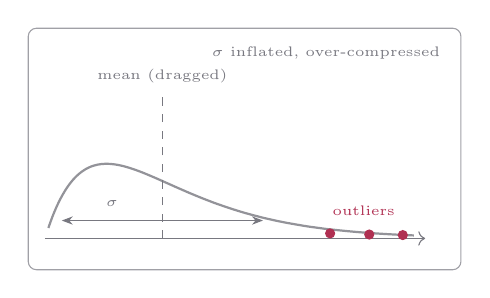
\begin{tikzpicture}[scale=1.42]
        \draw[->,soft] (0,0) -- (3.4,0);
        \draw[soft!80,thick,domain=0.03:3.3,samples=90,smooth]
          plot (\x,{6*\x*exp(-\x/0.55)*0.55});
        \draw[soft,dashed] (1.05,0) -- (1.05,1.28);
        \node[font=\tiny,soft,anchor=south] at (1.05,1.3) {mean (dragged)};
        \draw[{Stealth[length=1.4mm]}-{Stealth[length=1.4mm]},soft]
          (0.15,0.16) -- (1.95,0.16);
        \node[font=\tiny,soft,anchor=south] at (0.60,0.2) {$\sigma$};
        \fill[accent] (2.55,0.045) circle (1.3pt);
        \fill[accent] (2.9,0.035)  circle (1.3pt);
        \fill[accent] (3.2,0.03)   circle (1.3pt);
        \node[font=\tiny,accent,anchor=south] at (2.85,0.12) {outliers};
        \draw[soft!70, rounded corners=3pt, thin] (-0.15,-0.28) rectangle (3.72,1.88);
        \node[font=\tiny, text=soft, anchor=north east] at (3.62,1.80) {$\sigma$ inflated, over-compressed};
      \end{tikzpicture}
      \\[18pt]
      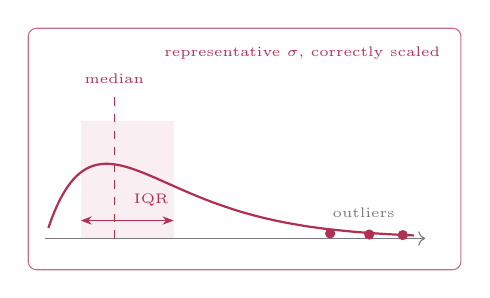
\begin{tikzpicture}[scale=1.42]
        \fill[accent!8] (0.32,0) rectangle (1.15,1.05);
        \draw[->,soft] (0,0) -- (3.4,0);
        \draw[accent,thick,domain=0.03:3.3,samples=90,smooth]
          plot (\x,{6*\x*exp(-\x/0.55)*0.55});
        \draw[accent,dashed] (0.62,0) -- (0.62,1.28);
        \node[font=\tiny,accent,anchor=south] at (0.62,1.3) {median};
        \draw[{Stealth[length=1.4mm]}-{Stealth[length=1.4mm]},accent]
          (0.32,0.16) -- (1.15,0.16);
        \node[font=\tiny,accent,anchor=south] at (0.95,0.2) {IQR};
        \fill[accent] (2.55,0.045) circle (1.3pt);
        \fill[accent] (2.9,0.035)  circle (1.3pt);
        \fill[accent] (3.2,0.03)   circle (1.3pt);
        \node[font=\tiny,soft,anchor=south] at (2.85,0.1) {outliers};
        \draw[accent!70, rounded corners=3pt, thin] (-0.15,-0.28) rectangle (3.72,1.88);
        \node[font=\tiny, text=accent, anchor=north east] at (3.62,1.80) {representative $\sigma$, correctly scaled};
      \end{tikzpicture}
    \end{column}
  \end{columns}
\end{frame}

% ---------------------------------------------------------------- 12b Normalization ablation ladder
\begin{frame}{Normalization ablation --- every rung improves, the output channels most}
    \centering
  \scriptsize
  \renewcommand{\arraystretch}{1.08}
  \setlength{\tabcolsep}{4pt}
  \renewcommand{\seedtag}{repA}
  \begin{tabular}{@{}l c c c !{\hspace{4pt}} c c@{}}
    \toprule
    metric & base & $+$pass mag & $+$ifg $\varphi$ & \textcolor{accent}{$+$out amp} & \textcolor{accent}{$+$out $\sigma$} \\
           &      & IQR\,log1p  & $\div\pi$        & \textcolor{accent}{IQR\,log1p}  & \textcolor{accent}{IQR\,log1p}    \\
    \midrule
    curve $R^2$ $\uparrow$            & \seedpm{0.51}{.04}   & \seedpm{0.53}{.01}   & \seedpm{0.54}{.01}   & \seedpm{\textbf{0.58}}{.03}   & \seedpm{0.57}{.02}           \\
    curve MAE $\downarrow$           & \seedpm{0.0572}{.003} & \seedpm{0.0544}{.001} & \seedpm{0.0531}{.001} & \seedpm{0.0504}{.002} & \seedpm{\textbf{0.0501}}{.001} \\
    PSNR [dB] $\uparrow$             & \seedpm{49.8}{.3}    & \seedpm{49.9}{.1}    & \seedpm{50.1}{.1}    & \seedpm{50.5}{.3}    & \seedpm{50.4}{.2}            \\
    per-pixel $R^2$ $\uparrow$        & \seedpm{0.070}{.015} & \seedpm{0.084}{.005} & \seedpm{0.091}{.004} & \seedpm{0.323}{.031}          & \seedpm{\hlval{good}{\textbf{0.359}}}{.050} \\
    profile cos med $\uparrow$        & \seedpm{0.000}{.000} & \seedpm{0.000}{.000} & \seedpm{0.000}{.000} & \seedpm{0.847}{.027}          & \seedpm{\hlval{good}{\textbf{0.851}}}{.020} \\
    \addlinespace
    SSIM elevation $\uparrow$        & \seedpm{0.953}{.002} & \seedpm{0.955}{.001} & \seedpm{0.956}{.001} & \seedpm{0.958}{.002}          & \seedpm{0.958}{.001} \\
    SSIM range $\uparrow$            & \seedpm{0.905}{.003} & \seedpm{0.907}{.001} & \seedpm{0.909}{.001} & \seedpm{0.923}{.001}          & \seedpm{0.926}{.003} \\
    SSIM azimuth $\uparrow$          & \seedpm{0.933}{.003} & \seedpm{0.935}{.001} & \seedpm{0.937}{.001} & \seedpm{0.944}{.002}          & \seedpm{0.946}{.001} \\
    \addlinespace
    matched F1 $\uparrow$            & \seedpm{0.467}{.009} & \seedpm{0.472}{.004} & \seedpm{0.476}{.003} & \seedpm{0.688}{.025}          & \seedpm{\hlval{good}{\textbf{0.727}}}{.040} \\
    matched recall $\uparrow$        & \seedpm{0.351}{.006} & \seedpm{0.354}{.004} & \seedpm{0.356}{.003} & \seedpm{0.604}{.036}          & \seedpm{\hlval{good}{\textbf{0.656}}}{.056} \\
    count exact $\uparrow$           & \seedpm{0.246}{.005} & \seedpm{0.246}{.005} & \seedpm{0.252}{.002} & \seedpm{0.547}{.050}          & \seedpm{\hlval{good}{\textbf{0.611}}}{.066} \\
    \addlinespace
    peak err mean $\downarrow$       & \seedpm{10.7}{.1}  & \seedpm{10.7}{.1}  & \seedpm{10.7}{.1}  & \seedpm{5.2}{.8}              & \seedpm{\hlval{good}{\textbf{4.5}}}{.9}   \\
    \quad median $\downarrow$        & \seedpm{13.7}{.4}  & \seedpm{13.8}{.4}  & \seedpm{13.7}{.4}  & \seedpm{1.2}{.6}              & \seedpm{\hlval{good}{\textbf{0.9}}}{.4}   \\
    \quad p95 $\downarrow$           & \seedpm{16.8}{.0}  & \seedpm{16.8}{.0}  & \seedpm{16.8}{.0}  & \seedpm{15.8}{.6}             & \seedpm{\textbf{15.4}}{.7}  \\
    matched $\mu$ MAE $\downarrow$   & \seedpm{3.44}{.09}   & \seedpm{3.37}{.05}   & \seedpm{3.30}{.02}   & \seedpm{2.47}{.10}            & \seedpm{\textbf{2.30}}{.12}  \\
    matched $\sigma$ MAE $\downarrow$ & \seedpm{1.39}{.03}  & \seedpm{1.36}{.02}   & \seedpm{1.34}{.01}   & \seedpm{0.96}{.04}            & \seedpm{\textbf{0.86}}{.05}  \\
    matched $a$ MAE $\downarrow$     & \seedpm{0.503}{.014} & \seedpm{0.503}{.008} & \seedpm{0.503}{.013} & \seedpm{0.383}{.020}          & \seedpm{\textbf{0.364}}{.034} \\
    \bottomrule
  \end{tabular}
  \par\vspace{3pt}
  \parbox{0.82\textwidth}{\tiny\color{soft} UNet $\cdot$ sorted-GT $\cdot$ $K{=}2$ $\cdot$ param-MSE $\cdot$ no aug $\cdot$ per-slot $\cdot$ patch $64{\times}32$; held-out validation band. Cells: mean $\pm$ seed std over five seeded replicas per rung. \textbf{bold} $=$ best in row, marked only where best and worst differ by more than $5\%$; \textcolor{accent}{red heads} $=$ the output rungs; \textcolor{good}{green} $=$ the metrics those rungs unlock. Base $=$ z-score outputs, zscore-log1p pass, minmax-$p99$ ifg (out $\mu$ stays z-score). $\mu$, $\sigma$, peak in elevation units; $a$ in linear amplitude. Peak median/p95: per-pixel peak-error distribution; profile cos med: median per-pixel cosine to the GT profile.\par}
    

\end{frame}

% ---------------------------------------------------------------- 12c Normalization ablation by scatterer count
\begin{frame}{Normalization ablation --- the gains concentrate on single-scatterer pixels}
    \centering
  \scriptsize
  \renewcommand{\arraystretch}{1.00}
  \setlength{\tabcolsep}{4pt}
  \renewcommand{\seedtag}{repB}
  \begin{tabular}{@{}l c c c !{\hspace{4pt}} c c@{}}
    \toprule
    metric & base & $+$pass mag & $+$ifg $\varphi$ & \textcolor{accent}{$+$out amp} & \textcolor{accent}{$+$out $\sigma$} \\
           &      & IQR\,log1p  & $\div\pi$        & \textcolor{accent}{IQR\,log1p}  & \textcolor{accent}{IQR\,log1p}    \\
    \midrule
    matched precision $\uparrow$ & \seedpm{0.699}{.015} & \seedpm{0.709}{.005} & \seedpm{0.720}{.005} & \seedpm{0.800}{.008} & \seedpm{\textbf{0.816}}{.015} \\
    \quad $k{=}1$                & \seedpm{0.602}{.015} & \seedpm{0.604}{.014} & \seedpm{0.624}{.005} & \seedpm{0.827}{.020} & \seedpm{\hlval{good}{\textbf{0.848}}}{.019} \\
    \quad $k{=}2$                & \seedpm{0.752}{.016} & \seedpm{0.765}{.007} & \seedpm{0.771}{.005} & \seedpm{0.767}{.017} & \seedpm{0.776}{.013} \\
    \addlinespace
    matched recall $\uparrow$    & \seedpm{0.351}{.006} & \seedpm{0.354}{.004} & \seedpm{0.356}{.003} & \seedpm{0.604}{.036} & \seedpm{\textbf{0.656}}{.056} \\
    \quad $k{=}1$                & \seedpm{0.182}{.006} & \seedpm{0.180}{.006} & \seedpm{0.182}{.004} & \seedpm{0.562}{.068} & \seedpm{\hlval{good}{\textbf{0.647}}}{.088} \\
    \quad $k{=}2$                & \seedpm{0.591}{.013} & \seedpm{0.602}{.007} & \seedpm{0.604}{.006} & \seedpm{0.663}{.014} & \seedpm{\textbf{0.670}}{.016} \\
    \addlinespace
    count acc $\mid$ pred $k{=}1$ $\uparrow$ & \seedpm{0.763}{.021} & \seedpm{0.781}{.015} & \seedpm{0.796}{.013} & \seedpm{0.942}{.009} & \seedpm{\hlval{good}{\textbf{0.952}}}{.009} \\
    count acc $\mid$ pred $k{=}2$ $\uparrow$ & \seedpm{0.694}{.008} & \seedpm{0.698}{.006} & \seedpm{0.711}{.007} & \seedpm{0.717}{.012} & \seedpm{0.720}{.013} \\
    \addlinespace
    matched $\mu$ MAE $\downarrow$ & \seedpm{3.44}{.09} & \seedpm{3.37}{.05} & \seedpm{3.30}{.02} & \seedpm{2.47}{.10} & \seedpm{\textbf{2.30}}{.12} \\
    \quad $k{=}1$                & \seedpm{1.25}{.06} & \seedpm{1.15}{.05} & \seedpm{1.10}{.03} & \seedpm{\textbf{0.63}}{.05} & \seedpm{\hlval{good}{\textbf{0.63}}}{.06} \\
    \quad $k{=}2$                & \seedpm{4.18}{.11} & \seedpm{4.10}{.04} & \seedpm{4.03}{.03} & \seedpm{4.17}{.10} & \seedpm{4.07}{.05} \\
    \addlinespace
    matched $\sigma$ MAE $\downarrow$ & \seedpm{1.39}{.03} & \seedpm{1.36}{.02} & \seedpm{1.34}{.01} & \seedpm{0.96}{.04} & \seedpm{\textbf{0.86}}{.05} \\
    \quad $k{=}1$                & \seedpm{0.61}{.02} & \seedpm{0.59}{.02} & \seedpm{0.59}{.01} & \seedpm{0.30}{.02} & \seedpm{\hlval{good}{\textbf{0.25}}}{.02} \\
    \quad $k{=}2$                & \seedpm{1.65}{.03} & \seedpm{1.61}{.01} & \seedpm{1.58}{.01} & \seedpm{1.58}{.04} & \seedpm{\textbf{1.51}}{.01} \\
    \addlinespace
    matched $a$ MAE $\downarrow$ & \seedpm{0.503}{.014} & \seedpm{0.503}{.008} & \seedpm{0.503}{.013} & \seedpm{0.383}{.020} & \seedpm{\textbf{0.364}}{.034} \\
    \quad $k{=}1$                & \seedpm{0.356}{.020} & \seedpm{0.359}{.016} & \seedpm{0.351}{.018} & \seedpm{0.169}{.018} & \seedpm{\hlval{good}{\textbf{0.155}}}{.029} \\
    \quad $k{=}2$                & \seedpm{0.552}{.012} & \seedpm{\textbf{0.550}}{.005} & \seedpm{0.554}{.011} & \seedpm{0.581}{.021} & \seedpm{\hlval{accent}{0.586}}{.035} \\
    \bottomrule
  \end{tabular}
  \par\vspace{3pt}
  \parbox{0.82\textwidth}{\tiny\color{soft} UNet $\cdot$ sorted-GT $\cdot$ $K{=}2$ $\cdot$ param-MSE $\cdot$ no aug $\cdot$ per-slot $\cdot$ patch $64{\times}32$; held-out validation band. Cells: mean $\pm$ seed std over five seeded replicas; $k$ $=$ true scatterer count of the pixel. \textbf{bold} $=$ best in row, marked only where best and worst differ by more than $5\%$; \textcolor{accent}{red heads} $=$ the output rungs; \textcolor{good}{green} $=$ the $k{=}1$ collapse they buy, \textcolor{accent}{red} $=$ the one drift up. Precision rewards under-prediction --- rank on recall. count acc $\mid$ pred $k$: share of pixels claiming exactly $k$ scatterers whose true count is $k$. $\mu$, $\sigma$ in elevation units; $a$ in linear amplitude.\par}
    

\end{frame}

% ---------------------------------------------------------------- 12d Normalization ablation: predicted stats vs GT
\begin{frame}{Normalization ablation --- slot 0 calibrates, slot 1 trades leakage against amplitude}
    \centering
  \scriptsize
  \renewcommand{\arraystretch}{1.02}
  \setlength{\tabcolsep}{2.5pt}
  \renewcommand{\seedtag}{repC}
  \begin{tabular}{@{}l c !{\color{white}\vrule width 1.6pt} c c c !{\hspace{2pt}} c c@{}}
    \toprule
    prediction mean & \textcolor{good}{GT} & base & $+$pass mag & $+$ifg $\varphi$ & \textcolor{accent}{$+$out amp} & \textcolor{accent}{$+$out $\sigma$} \\
                    &                      &      & IQR\,log1p  & $\div\pi$        & \textcolor{accent}{IQR\,log1p}  & \textcolor{accent}{IQR\,log1p}    \\
    \midrule
    \multicolumn{7}{@{}l}{\textcolor{soft}{\emph{slot 0 --- strongest scatterer; GT-active on every pixel}}} \\
    \quad active frac            & 1.00    & \seedpm{0.344}{.004} & \seedpm{0.342}{.004} & \seedpm{0.342}{.003} & \seedpm{0.644}{.051} & \seedpm{\hlval{good}{\textbf{0.706}}}{.066} \\
    \quad $a$ --- active      & 0.77    & \seedpm{1.87}{.03}   & \seedpm{1.88}{.03}   & \seedpm{1.87}{.01}   & \seedpm{0.98}{.08}   & \seedpm{\hlval{good}{\textbf{0.89}}}{.07}   \\
    \quad $\mu$ --- active    & $-4.89$ & \seedpm{$-3.73$}{.10} & \seedpm{$-3.58$}{.07} & \seedpm{$-3.59$}{.02} & \seedpm{$-4.00$}{.09} & \seedpm{\textbf{$-4.03$}}{.15} \\
    \quad $\sigma$ --- active & 1.76    & \seedpm{2.36}{.05}   & \seedpm{2.31}{.05}   & \seedpm{2.36}{.03}   & \seedpm{\textbf{1.73}}{.04} & \seedpm{\hlval{accent}{1.52}}{.08} \\
    \addlinespace
    \multicolumn{7}{@{}l}{\textcolor{soft}{\emph{slot 1 --- second scatterer; GT-active on 26\% of pixels}}} \\
    \quad active frac            & 0.260 & \seedpm{0.289}{.005} & \seedpm{0.288}{.004} & \seedpm{\textbf{0.281}}{.003} & \seedpm{0.308}{.007} & \seedpm{0.306}{.008} \\
    \quad $a$ --- active      & 1.43  & \seedpm{1.33}{.04} & \seedpm{1.33}{.03} & \seedpm{\textbf{1.34}}{.03} & \seedpm{1.04}{.04} & \seedpm{1.06}{.05} \\
    \quad $a$ --- inact.    & 0.00  & \seedpm{0.74}{.03} & \seedpm{0.70}{.03} & \seedpm{0.68}{.01} & \seedpm{\hlval{good}{\textbf{0.44}}}{.02} & \seedpm{0.45}{.04} \\
    \quad $\mu$ --- active    & 11.34 & \seedpm{10.39}{.39} & \seedpm{10.20}{.38} & \seedpm{\textbf{10.56}}{.32} & \seedpm{10.23}{.48} & \seedpm{9.97}{.40} \\
    \quad $\mu$ --- inact.  & ---   & \seedpm{3.66}{.31} & \seedpm{3.65}{.26} & \seedpm{3.98}{.24} & \seedpm{3.73}{.72} & \seedpm{3.39}{.57} \\
    \quad $\sigma$ --- active & 3.53  & \seedpm{3.59}{.10} & \seedpm{\textbf{3.52}}{.09} & \seedpm{3.58}{.06} & \seedpm{3.41}{.11} & \seedpm{3.02}{.04} \\
    \quad $\sigma$ --- inact. & --- & \seedpm{2.36}{.10} & \seedpm{2.27}{.05} & \seedpm{2.21}{.02} & \seedpm{2.06}{.06} & \seedpm{1.90}{.04} \\
    \addlinespace
    \multicolumn{7}{@{}l}{\textcolor{soft}{\emph{distribution width --- std over GT-active pixels}}} \\
    \quad $a$ --- slot 0      & 1.48  & \seedpm{1.43}{.04} & \seedpm{\textbf{1.44}}{.04} & \seedpm{1.42}{.04} & \seedpm{1.24}{.07} & \seedpm{1.17}{.06} \\
    \quad $\mu$ --- slot 0    & 3.30  & \seedpm{2.27}{.10} & \seedpm{2.31}{.08} & \seedpm{\textbf{2.38}}{.05} & \seedpm{2.07}{.08} & \seedpm{2.03}{.12} \\
    \quad $\sigma$ --- slot 0 & 2.84  & \seedpm{0.95}{.05} & \seedpm{0.95}{.05} & \seedpm{1.07}{.06} & \seedpm{\textbf{1.30}}{.05} & \seedpm{1.01}{.03} \\
    \quad $a$ --- slot 1      & 1.45  & \seedpm{0.92}{.03} & \seedpm{0.94}{.04} & \seedpm{\textbf{0.95}}{.03} & \seedpm{0.83}{.04} & \seedpm{0.84}{.05} \\
    \quad $\mu$ --- slot 1    & 16.24 & \seedpm{7.28}{.23} & \seedpm{7.26}{.21} & \seedpm{7.55}{.23} & \seedpm{8.65}{.29} & \seedpm{\textbf{8.76}}{.27} \\
    \quad $\sigma$ --- slot 1 & 4.01  & \seedpm{1.11}{.05} & \seedpm{1.11}{.03} & \seedpm{1.19}{.04} & \seedpm{\textbf{1.35}}{.08} & \seedpm{1.14}{.04} \\
    \bottomrule
  \end{tabular}
  \par\vspace{3pt}
  \parbox{0.82\textwidth}{\tiny\color{soft} UNet $\cdot$ sorted-GT $\cdot$ $K{=}2$ $\cdot$ param-MSE $\cdot$ no aug $\cdot$ per-slot $\cdot$ patch $64{\times}32$; held-out validation band. Cells: mean $\pm$ seed std over five seeded replicas; means conditioned on the slot's GT activity mask. \textbf{bold} $=$ closest to the \textcolor{good}{GT} column, marked only where best and worst differ by more than $5\%$; \textcolor{good}{green} $=$ the calibration shifts that matter, \textcolor{accent}{red} $=$ the one overshoot past the GT. Inactive GT slots define no $\mu$/$\sigma$ reference (---). Width rows: std of the prediction over GT-active pixels vs the GT's own std. $\mu$, $\sigma$ in elevation units; $a$ in linear amplitude.\par}
    

\end{frame}


\act{III \ \ Training method}{set matching \; $\cdot$ \; slot imbalance \; $\cdot$ \; stability}
\subact{Failure modes}{exponential loss \; $\cdot$ \; permutation invariance \; $\cdot$ \; capacity \; $\cdot$ \; sorting \; $\cdot$ \; class imbalance \; $\cdot$ \; overfitting}

% ---------------------------------------------------------------- 13-i Why clamp --- the exponential overflow
\begin{frame}{Why clamp the output --- the exponential overflows}
  \small
  \begin{columns}[c]
    \begin{column}{0.54\textwidth}
      \begin{center}
        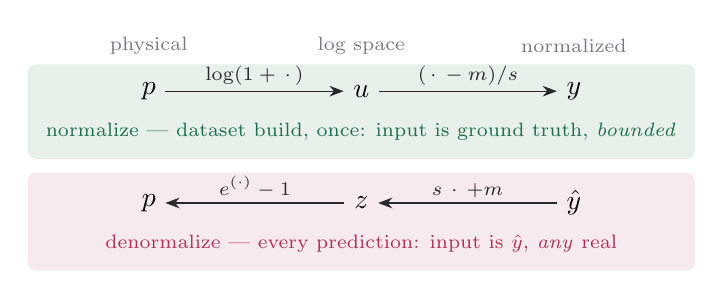
\begin{tikzpicture}
          \node[font=\scriptsize, text=soft] at (0,0.58)   {physical};
          \node[font=\scriptsize, text=soft] at (2.7,0.58) {log space};
          \node[font=\scriptsize, text=soft] at (5.4,0.58) {normalized};

          \node (n0) at (0,0)   {$p$};
          \node (n1) at (2.7,0) {$u$};
          \node (n2) at (5.4,0) {$y$};
          \draw[-{Stealth[length=1.8mm]}, ink] (n0) -- (n1) node[midway, above=-1.5pt, font=\scriptsize] {$\log(1+\,\cdot\,)$};
          \draw[-{Stealth[length=1.8mm]}, ink] (n1) -- (n2) node[midway, above=-1.5pt, font=\scriptsize] {$(\,\cdot\,-m)/s$};
          \node[font=\scriptsize, text=good] (ncap) at (2.7,-0.52) {normalize --- dataset build, once: input is ground truth, \emph{bounded}};

          \node (d0) at (0,-1.42)   {$p$};
          \node (d1) at (2.7,-1.42) {$z$};
          \node (d2) at (5.4,-1.42) {$\hat y$};
          \draw[{Stealth[length=1.8mm]}-, ink] (d0) -- (d1) node[midway, above=-1.5pt, font=\scriptsize] {$e^{(\cdot)}-1$};
          \draw[{Stealth[length=1.8mm]}-, ink] (d1) -- (d2) node[midway, above=-1.5pt, font=\scriptsize] {$s\,\cdot\,+m$};
          \node[font=\scriptsize, text=accent] (dcap) at (2.7,-1.94) {denormalize --- every prediction: input is $\hat y$, \emph{any} real};

          \begin{scope}[on background layer]
            \node[fill=good!10, rounded corners=3pt, inner sep=3pt,
                  fit=(n0)(n1)(n2)(ncap)(dcap.west |- ncap.center)(dcap.east |- ncap.center)] {};
            \node[fill=accent!10, rounded corners=3pt, inner sep=3pt,
                  fit=(d0)(d1)(d2)(dcap)(ncap.west |- dcap.center)(ncap.east |- dcap.center)] {};
          \end{scope}
        \end{tikzpicture}
      \end{center}
      {\scriptsize $p\!\in\!\{a,\sigma\}$ ($\mu$ skips the log --- linear both ways);\;
       $m,s$: fixed channel shift \& scale. Composed:\; $p = e^{s\hat y + m}-1$.}

      \vspace{4pt}
      \begin{center}
        $\displaystyle
         \begin{aligned}
           \hat y \to \infty \ &\Longrightarrow\ z \to \infty \\[2pt]
           &\Longrightarrow\ p = e^{z}-1 \to \infty \\[2pt]
           &\Longrightarrow\ \mathcal{L} \to \infty \\[2pt]
           &\Longrightarrow\ \nabla_{\!\theta}\mathcal{L} = \mathrm{NaN}
         \end{aligned}$
      \end{center}
      {\scriptsize $\mathcal{L}$: training loss,\; $\theta$: weights. One overflowing pixel
       $\Rightarrow$ every weight NaN $\Rightarrow$ \textbf{no} training.}
    \end{column}
    \begin{column}{0.46\textwidth}
      \begin{center}
        $\boxed{\ p \;=\; e^{\min(z,\,h)}-1 \ \le\ p_{\max}\ }$
      \end{center}
      {\scriptsize $h=\log(1+p_{\max})$,\; $p_{\max}$: physical ceiling. The front-end
       \texttt{clamp} toggle --- off $\Rightarrow$ overflow returns.}

      \vspace{6pt}
      \begin{center}
      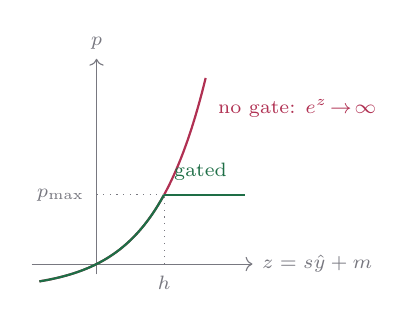
\begin{tikzpicture}[scale=0.66]
        \draw[->, soft] (-1.25,0) -- (3.0,0) node[right, font=\scriptsize] {$z = s\hat y + m$};
        \draw[->, soft] (0,-0.2) -- (0,3.95) node[above, font=\scriptsize] {$p$};
        \draw[accent, thick, domain=-1.1:2.1, smooth, samples=60] plot (\x, {0.5*(exp(\x)-1)});
        \draw[good, thick, domain=-1.1:1.3, smooth, samples=40] plot (\x, {0.5*(exp(\x)-1)});
        \draw[good, thick] (1.3,1.331) -- (2.85,1.331);
        \draw[soft, dotted] (1.3,0) -- (1.3,1.331);
        \draw[soft, dotted] (0,1.331) -- (1.3,1.331);
        \node[soft, font=\scriptsize, anchor=north] at (1.3,-0.04) {$h$};
        \node[soft, font=\scriptsize, anchor=east] at (-0.05,1.331) {$p_{\max}$};
        \node[accent, font=\scriptsize, anchor=west] at (2.15,3.0) {no gate: $e^{z}\!\to\!\infty$};
        \node[good, font=\scriptsize, anchor=south] at (2.0,1.42) {gated};
      \end{tikzpicture}
      \end{center}
      \centering
      {\scriptsize\itshape unbounded $e^{z}$ (red) vs.\ exponent gated at $h$ (green)}
    \end{column}
  \end{columns}
\end{frame}

% ---------------------------------------------------------------- 13-ii Leaky clamp
\begin{frame}{The leaky clamp --- stability keystone}
  \small
  \begin{columns}[c]
    \begin{column}{0.44\textwidth}
      One unphysical parameter (negative $\sigma$, runaway $a$, off-grid $\mu$)
      poisons every loss term downstream; a hard clamp fixes the forward pass but
      kills the gradient. The leaky clamp bounds the value \emph{and} keeps a slope.
      \vspace{12pt}
      \begin{center}
      {\scriptsize\itshape forward pass --- the clamp guards the loss path}\\[8pt]
      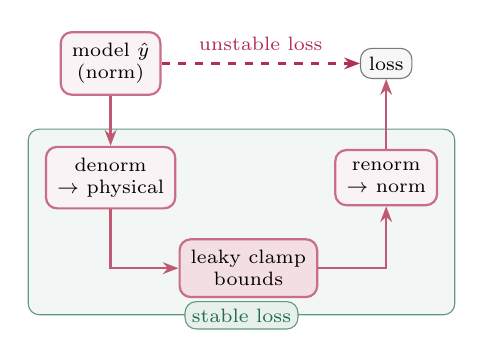
\begin{tikzpicture}
        \node[box] (m) at (0,0)        {model $\hat y$\\{\scriptsize (norm)}};
        \node[box] (d) at (0,-1.45)    {denorm\\{\scriptsize $\to$ physical}};
        \node[box, fill=accent!16] (c) at (1.75,-2.6) {leaky clamp\\{\scriptsize bounds}};
        \node[box] (r) at (3.5,-1.45)  {renorm\\{\scriptsize $\to$ norm}};
        \node[gate] (l) at (3.5,0)     {loss};
        \begin{scope}[on background layer]
          \node[draw=good!70, fill=good!6, rounded corners, inner sep=6pt, fit=(d)(c)(r)] (stab) {};
        \end{scope}
        \draw[flow] (m) -- (d);
        \draw[flow] (d.south) |- (c.west);
        \draw[flow] (c.east) -| (r.south);
        \draw[flow] (r) -- (l);
        \draw[-{Stealth[length=2mm]}, accent, thick, dashed] (m.east) -- (l.west)
          node[midway, above=1pt, font=\scriptsize, text=accent] {unstable loss};
        \node[draw=good!70, fill=good!10, rounded corners, inner sep=2.5pt,
              font=\scriptsize, text=good] at (stab.south) {stable loss};
      \end{tikzpicture}
      \end{center}
    \end{column}
    \begin{column}{0.54\textwidth}
      \centering
      $\boxed{\ \tilde x = \mathrm{clamp}(x) + \lambda\,\big(x-\mathrm{clamp}(x)\big)\ }$\\[5pt]
      {\scriptsize $a\!\in\![0,a_{\max}]$,\; $\mu\!\in\![x_{\min},x_{\max}]$,\;
       $\sigma\!\in\![\tfrac12 x_\text{step},\tfrac12 x_\text{range}]$}

      \vspace{12pt}
      {\scriptsize\itshape one outlier prediction $x$ (pushed off physical bounds)}\\[3pt]
      {\scriptsize
      \renewcommand{\arraystretch}{1.1}
      \setlength{\tabcolsep}{6pt}
      \begin{tabular}{@{}lll@{}}
        \toprule
        on the outlier & loss & gradient $\partial\mathcal{L}/\partial x$ \\
        \midrule
        no clamp   & \textcolor{accent}{$\infty$ / NaN} & \textcolor{accent}{poisons all terms} \\
        hard clamp & \textcolor{good}{bounded}          & \textcolor{accent}{$0$ --- slot dies} \\
        \rowcolor{good!12} leaky clamp & \textcolor{good}{bounded}
                   & \textcolor{good}{$\lambda\!>\!0$ --- keeps signal} \\
        \bottomrule
      \end{tabular}}

      \vspace{12pt}
      \begin{minipage}[t]{0.49\linewidth}
        \centering
        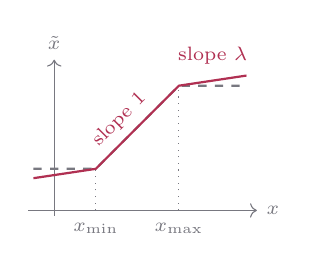
\begin{tikzpicture}[scale=0.66]
          \draw[->, soft] (-0.5,0) -- (3.9,0) node[right, font=\scriptsize] {$x$};
          \draw[->, soft] (0,-0.1) -- (0,2.9) node[above, font=\scriptsize] {$\tilde x$};
          \draw[soft, dotted] (0.8,0) -- (0.8,0.8);
          \draw[soft, dotted] (2.4,0) -- (2.4,2.4);
          \node[font=\scriptsize, text=soft, anchor=north] at (0.8,-0.05) {$x_{\min}$};
          \node[font=\scriptsize, text=soft, anchor=north] at (2.4,-0.05) {$x_{\max}$};
          \draw[soft, thick, dashed] (-0.4,0.8) -- (0.8,0.8) -- (2.4,2.4) -- (3.7,2.4);
          \draw[accent, thick] (-0.4,0.62) -- (0.8,0.8) -- (2.4,2.4) -- (3.7,2.595);
          \node[font=\scriptsize, text=accent, rotate=45] at (1.25,1.75) {slope $1$};
          \node[font=\scriptsize, text=accent, anchor=south] at (3.05,2.62) {slope $\lambda$};
        \end{tikzpicture}
        \\[2pt]
        {\scriptsize value: \textcolor{accent}{training, leaky} vs
         \textcolor{soft}{inference, hard ($\lambda=0$)}}
      \end{minipage}\hfill
      \begin{minipage}[t]{0.49\linewidth}
        \centering
        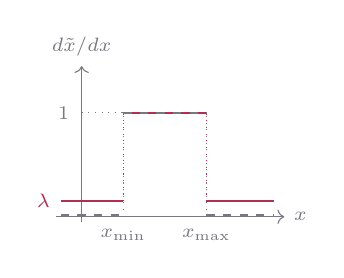
\begin{tikzpicture}[scale=0.66]
          \draw[->, soft] (-0.5,0) -- (3.9,0) node[right, font=\scriptsize] {$x$};
          \draw[->, soft] (0,-0.1) -- (0,2.9) node[above, font=\scriptsize] {$d\tilde x/dx$};
          \draw[soft, dotted] (0.8,0) -- (0.8,2.0);
          \draw[soft, dotted] (2.4,0) -- (2.4,2.0);
          \node[font=\scriptsize, text=soft, anchor=north] at (0.8,-0.05) {$x_{\min}$};
          \node[font=\scriptsize, text=soft, anchor=north] at (2.4,-0.05) {$x_{\max}$};
          \draw[soft, dotted] (0,2.0) -- (0.8,2.0);
          \node[font=\scriptsize, text=soft, anchor=east] at (-0.05,2.0) {$1$};
          \node[font=\scriptsize, text=accent, anchor=east] at (-0.42,0.3) {$\lambda$};
          \draw[soft, thick, dashed] (-0.4,0.04) -- (0.8,0.04);
          \draw[soft, thick, dashed] (2.4,0.04) -- (3.7,0.04);
          \draw[accent, thick] (-0.4,0.3) -- (0.8,0.3);
          \draw[accent, thick] (0.8,2.0) -- (2.4,2.0);
          \draw[accent, thick] (2.4,0.3) -- (3.7,0.3);
          \draw[soft, thick, dashed] (0.8,2.0) -- (2.4,2.0);
          \draw[accent, thin, dotted] (0.8,0.3) -- (0.8,2.0);
          \draw[accent, thin, dotted] (2.4,0.3) -- (2.4,2.0);
        \end{tikzpicture}
        \\[2pt]
        {\scriptsize gradient: never zero --- saturated slots keep receiving signal}
      \end{minipage}
    \end{column}
  \end{columns}
\end{frame}

% ---------------------------------------------------------------- 13-iii Warmup + adaptive gradient clipping
\begin{frame}{LR warmup and adaptive gradient clipping}
  \small
  \begin{columns}[c]
    \begin{column}{0.36\textwidth}
      \hspace*{5mm}\begin{minipage}{\dimexpr\linewidth-5mm\relax}
      \footnotesize
      \begin{itemize}
        \item A linear \textbf{warmup} over the first 200 steps tames the early,
              high-variance gradients, then epoch-level cosine annealing down to
              $\eta_{\min}$.
              {\scriptsize\[\begin{aligned}
                 \eta(t,s)        &= \eta_0 \, F_{\cos}(t)\, f_{\text{warm}}(s)\\[6pt]
                 f_{\text{warm}}(s) &= 0.1 + 0.9\,\min\!\big(1,\ s/t_{\text{warm}}\big)\\[6pt]
                 F_{\cos}(t)       &= \tfrac12\big(1+\cos(\pi (t-t_{\text{warm}})/T)\big)
               \end{aligned}\]}
      \end{itemize}
      \end{minipage}
    \end{column}
    \begin{column}{0.62\textwidth}
      \hspace*{2mm}%
      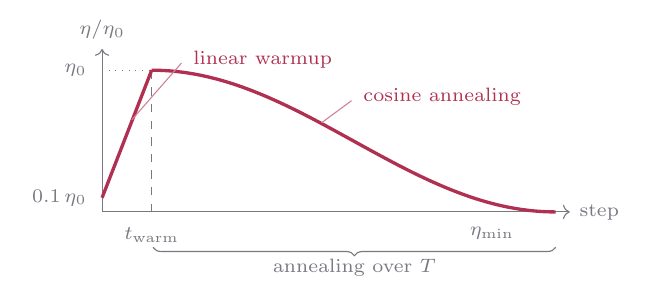
\begin{tikzpicture}[scale=0.9]
    \useasboundingbox (-1.05,-0.85) rectangle (7.5,2.6);
    \draw[->,soft] (0,0) -- (6.6,0) node[right,font=\scriptsize]{step};
    \draw[->,soft] (0,0) -- (0,2.3) node[above,font=\scriptsize]{$\eta/\eta_0$};
    \draw[soft,dashed] (0.7,0) -- (0.7,2.0);
    \draw[soft,dotted] (0,2.0) -- (0.7,2.0);
    \draw[accent,very thick] (0,0.2) -- (0.7,2.0);
    \draw[accent,very thick,domain=0.7:6.4,samples=90,smooth]
      plot (\x,{2.0*0.5*(1+cos(180*(\x-0.7)/5.7))});
    \node[font=\scriptsize,soft,anchor=east]  at (-0.08,2.0)  {$\eta_0$};
    \node[font=\scriptsize,soft,anchor=east]  at (-0.08,0.2)  {$0.1\,\eta_0$};
    \node[font=\scriptsize,soft,anchor=north] at (0.7,-0.08)  {$t_{\text{warm}}$};
    \node[font=\scriptsize,soft,anchor=north] at (5.5,-0.08)  {$\eta_{\min}$};
    \draw[decorate,decoration={brace,amplitude=3pt,mirror},soft] (0.72,-0.5) -- (6.4,-0.5);
    \node[font=\scriptsize,soft,anchor=north] at (3.56,-0.52) {annealing over $T$};
    \node[font=\scriptsize,accent,anchor=west] at (1.15,2.15) {linear warmup};
    \draw[accent!60,thin] (1.12,2.1) -- (0.42,1.3);
    \node[font=\scriptsize,accent,anchor=west] at (3.55,1.62) {cosine annealing};
    \draw[accent!60,thin] (3.52,1.57) -- (3.1,1.26);
      \end{tikzpicture}
    \end{column}
  \end{columns}
  \vspace{6pt}
  \begin{columns}[c]
    \begin{column}{0.36\textwidth}
      \hspace*{5mm}\begin{minipage}{\dimexpr\linewidth-5mm\relax}
      \footnotesize
      \begin{itemize}
        \item Rolling window of the last 200 global gradient norms, threshold
              recomputed every step as the p95 of the window --- the first $\sim$200
              steps only observe; this avoids starving the gradients ---
              a training insurance.
              {\scriptsize\[\begin{aligned}
                 \tau_t  &= \mathrm{p95}\big(\{\lVert g\rVert\}_{t-200:t}\big)\\[6pt]
                 g       &\leftarrow g \cdot \min\!\big(1,\ \tau_t/\lVert g\rVert\big)
               \end{aligned}\]}
      \end{itemize}
      \end{minipage}
    \end{column}
    \begin{column}{0.62\textwidth}
      \hspace*{2mm}%
      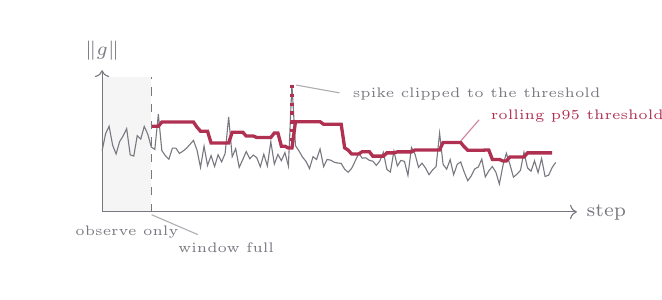
\begin{tikzpicture}[scale=0.9]
    \useasboundingbox (-1.05,-0.85) rectangle (7.5,2.6);
    \fill[black!4] (0,0) rectangle (0.695,1.9);
    \draw[->,soft] (0,0) -- (6.7,0) node[right,font=\scriptsize]{step};
    \draw[->,soft] (0,0) -- (0,2.0) node[above,font=\scriptsize]{$\lVert g \rVert$};
    \draw[soft,thin] plot coordinates {(0.000,0.863) (0.050,1.105) (0.099,1.209) (0.149,0.941) (0.198,0.818) (0.248,0.993) (0.298,1.074) (0.347,1.175) (0.397,0.805) (0.447,0.788) (0.496,1.076) (0.546,1.028) (0.595,1.207) (0.645,1.096) (0.695,0.914) (0.744,0.882) (0.794,1.379) (0.843,0.866) (0.893,0.794) (0.943,0.744) (0.992,0.900) (1.042,0.900) (1.091,0.826) (1.141,0.857) (1.191,0.898) (1.240,0.953) (1.290,1.009) (1.340,0.870) (1.389,0.627) (1.439,0.928) (1.488,0.656) (1.538,0.795) (1.588,0.641) (1.637,0.807) (1.687,0.707) (1.736,0.824) (1.786,1.341) (1.836,0.779) (1.885,0.893) (1.935,0.628) (1.984,0.736) (2.034,0.852) (2.084,0.750) (2.133,0.803) (2.183,0.765) (2.233,0.637) (2.282,0.814) (2.332,0.649) (2.381,0.992) (2.431,0.674) (2.481,0.811) (2.530,0.723) (2.580,0.837) (2.629,0.649) (2.679,1.794) (2.729,0.936) (2.778,0.862) (2.828,0.774) (2.878,0.713) (2.927,0.612) (2.977,0.780) (3.026,0.740) (3.076,0.889) (3.126,0.640) (3.175,0.740) (3.225,0.731) (3.274,0.702) (3.324,0.690) (3.374,0.685) (3.423,0.602) (3.473,0.560) (3.522,0.616) (3.572,0.718) (3.622,0.829) (3.671,0.758) (3.721,0.764) (3.771,0.728) (3.820,0.716) (3.870,0.657) (3.919,0.719) (3.969,0.841) (4.019,0.599) (4.068,0.563) (4.118,0.857) (4.167,0.649) (4.217,0.727) (4.267,0.713) (4.316,0.515) (4.366,0.909) (4.416,0.815) (4.465,0.629) (4.515,0.688) (4.564,0.620) (4.614,0.526) (4.664,0.593) (4.713,0.639) (4.763,1.112) (4.812,0.671) (4.862,0.603) (4.912,0.739) (4.961,0.525) (5.011,0.672) (5.060,0.705) (5.110,0.562) (5.160,0.441) (5.209,0.507) (5.259,0.607) (5.309,0.634) (5.358,0.745) (5.408,0.494) (5.457,0.579) (5.507,0.640) (5.557,0.561) (5.606,0.393) (5.656,0.652) (5.705,0.828) (5.755,0.670) (5.805,0.491) (5.854,0.532) (5.904,0.587) (5.953,0.842) (6.003,0.623) (6.053,0.574) (6.102,0.721) (6.152,0.554) (6.202,0.754) (6.251,0.501) (6.301,0.517) (6.350,0.625) (6.400,0.698)};
    \draw[accent,very thick] plot coordinates {(0.695,1.208) (0.744,1.208) (0.794,1.208) (0.843,1.268) (0.893,1.268) (0.943,1.268) (0.992,1.268) (1.042,1.268) (1.091,1.268) (1.141,1.268) (1.191,1.268) (1.240,1.268) (1.290,1.268) (1.340,1.195) (1.389,1.139) (1.439,1.139) (1.488,1.139) (1.538,0.973) (1.588,0.973) (1.637,0.973) (1.687,0.973) (1.736,0.973) (1.786,0.973) (1.836,1.125) (1.885,1.125) (1.935,1.125) (1.984,1.125) (2.034,1.072) (2.084,1.072) (2.133,1.072) (2.183,1.050) (2.233,1.050) (2.282,1.050) (2.332,1.050) (2.381,1.050) (2.431,1.114) (2.481,1.114) (2.530,0.928) (2.580,0.928) (2.629,0.901) (2.679,0.901) (2.729,1.273) (2.778,1.273) (2.828,1.273) (2.878,1.273) (2.927,1.273) (2.977,1.273) (3.026,1.273) (3.076,1.273) (3.126,1.237) (3.175,1.237) (3.225,1.237) (3.274,1.237) (3.324,1.237) (3.374,1.237) (3.423,0.905) (3.473,0.871) (3.522,0.818) (3.572,0.818) (3.622,0.818) (3.671,0.850) (3.721,0.850) (3.771,0.850) (3.820,0.787) (3.870,0.787) (3.919,0.787) (3.969,0.787) (4.019,0.833) (4.068,0.833) (4.118,0.833) (4.167,0.847) (4.217,0.847) (4.267,0.847) (4.316,0.847) (4.366,0.847) (4.416,0.875) (4.465,0.875) (4.515,0.875) (4.564,0.875) (4.614,0.875) (4.664,0.875) (4.713,0.875) (4.763,0.875) (4.812,0.980) (4.862,0.980) (4.912,0.980) (4.961,0.980) (5.011,0.980) (5.060,0.980) (5.110,0.919) (5.160,0.870) (5.209,0.870) (5.259,0.870) (5.309,0.870) (5.358,0.870) (5.408,0.873) (5.457,0.873) (5.507,0.741) (5.557,0.741) (5.606,0.741) (5.656,0.719) (5.705,0.719) (5.755,0.774) (5.805,0.774) (5.854,0.774) (5.904,0.774) (5.953,0.774) (6.003,0.833) (6.053,0.833) (6.102,0.833) (6.152,0.833) (6.202,0.833) (6.251,0.833) (6.301,0.833) (6.350,0.833)};
    \draw[accent,dotted,very thick] (2.679,1.794) -- (2.679,0.92);
    \draw[soft,dashed] (0.695,0) -- (0.695,1.9);
    \draw[soft!60,thin] (3.35,1.68) -- (2.74,1.79);
    \node[font=\tiny,soft,anchor=west]  at (3.4,1.66)   {spike clipped to the threshold};
    \node[font=\tiny,soft,anchor=north] at (0.35,-0.06) {observe only};
    \node[font=\tiny,soft,anchor=north] at (1.75,-0.3)  {window full};
    \draw[soft!60,thin] (1.35,-0.32) -- (0.7,-0.04);
    \node[font=\tiny,accent,anchor=west] at (5.35,1.35) {rolling p95 threshold};
    \draw[accent!60,thin] (5.32,1.30) -- (5.06,1.00);
      \end{tikzpicture}
    \end{column}
  \end{columns}
\end{frame}

% ---------------------------------------------------------------- 13a Small-K failure example
\begin{frame}{The small-$K$ failure, concretely ($K{=}2$)}
  \small
  \begin{columns}[c]
    \begin{column}{0.42\textwidth}
      \footnotesize
      \begin{itemize}
        \setlength{\itemsep}{10pt}
        \item Most pixels hold ground + canopy --- the network internalises that
              prior: slot 2 \emph{expects} a canopy.
        \item Here a mid-height volume outshines the canopy. GT extraction keeps the
              $K$ strongest components, so the volume \emph{becomes} the second
              Gaussian --- the canopy leaves the label entirely.
        \item The prior misfires: slot 2 lands at canopy height while the label holds
              the volume --- a \textbf{capacity failure of small $K$}: the label
              itself has no room for a third layer.
        \item At larger $K$ a different failure appears: the sorting mechanism itself
              (two frames ahead).
      \end{itemize}
    \end{column}
    \begin{column}{0.56\textwidth}
      \centering
      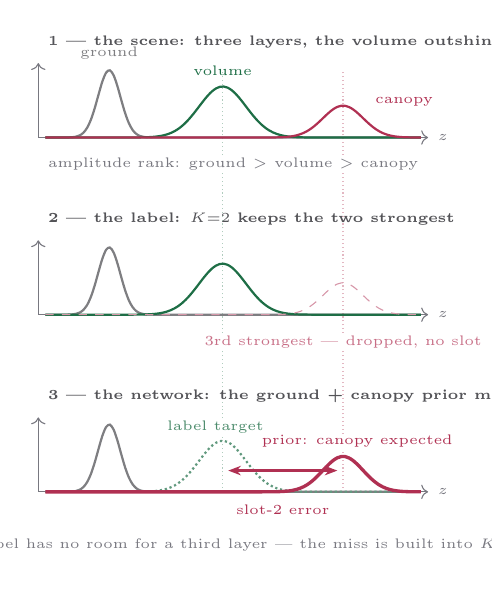
\begin{tikzpicture}[scale=0.9]
    \useasboundingbox (-0.15,-6.0) rectangle (6.0,1.55);
    \draw[good!35,densely dotted]   (2.6,-5.0) -- (2.6,0.95);
    \draw[accent!35,densely dotted] (4.3,-5.0) -- (4.3,0.95);
    \node[font=\tiny\bfseries,ink!80,anchor=west] at (0,1.35)
      {1 --- the scene: three layers, the volume outshines the canopy};
    \draw[->,soft] (0,0) -- (5.5,0) node[right,font=\tiny]{$z$};
    \draw[->,soft] (0,0) -- (0,1.05);
    \draw[ink!60,thick,domain=0.1:5.4,samples=100,smooth]
      plot (\x,{0.95*exp(-(\x-1.0)^2/0.05)});
    \draw[good,thick,domain=0.1:5.4,samples=100,smooth]
      plot (\x,{0.72*exp(-(\x-2.6)^2/0.22)});
    \draw[accent,thick,domain=0.1:5.4,samples=100,smooth]
      plot (\x,{0.45*exp(-(\x-4.3)^2/0.16)});
    \node[font=\tiny,ink!60,anchor=south] at (1.0,0.97)  {ground};
    \node[font=\tiny,good,anchor=south]   at (2.6,0.74)  {volume};
    \node[font=\tiny,accent,anchor=west]  at (4.62,0.5)  {canopy};
    \node[font=\tiny,soft,fill=white,inner sep=0.5pt] at (2.75,-0.38)
      {amplitude rank: ground $>$ volume $>$ canopy};
    \node[font=\tiny\bfseries,ink!80,anchor=west] at (0,-1.15)
      {2 --- the label: $K{=}2$ keeps the two strongest};
    \draw[->,soft] (0,-2.5) -- (5.5,-2.5) node[right,font=\tiny]{$z$};
    \draw[->,soft] (0,-2.5) -- (0,-1.45);
    \draw[ink!60,thick,domain=0.1:5.4,samples=100,smooth]
      plot (\x,{-2.5+0.95*exp(-(\x-1.0)^2/0.05)});
    \draw[good,thick,domain=0.1:5.4,samples=100,smooth]
      plot (\x,{-2.5+0.72*exp(-(\x-2.6)^2/0.22)});
    \draw[accent!50,thin,dashed,domain=0.1:5.4,samples=100,smooth]
      plot (\x,{-2.5+0.45*exp(-(\x-4.3)^2/0.16)});
    \node[font=\tiny,accent!70,fill=white,inner sep=0.5pt] at (4.3,-2.88)
      {3rd strongest --- dropped, no slot};
    \node[font=\tiny\bfseries,ink!80,anchor=west] at (0,-3.65)
      {3 --- the network: the ground + canopy prior misfires};
    \draw[->,soft] (0,-5.0) -- (5.5,-5.0) node[right,font=\tiny]{$z$};
    \draw[->,soft] (0,-5.0) -- (0,-3.95);
    \draw[ink!60,thick,domain=0.1:5.4,samples=100,smooth]
      plot (\x,{-5.0+0.95*exp(-(\x-1.0)^2/0.05)});
    \draw[good!70,thick,densely dotted,domain=0.1:5.4,samples=100,smooth]
      plot (\x,{-5.0+0.72*exp(-(\x-2.6)^2/0.22)});
    \draw[accent,very thick,domain=0.1:5.4,samples=100,smooth]
      plot (\x,{-5.0+0.5*exp(-(\x-4.3)^2/0.16)});
    \node[font=\tiny,good!80,anchor=south,fill=white,inner sep=0.5pt] at (2.5,-4.2) {label target};
    \node[font=\tiny,accent,anchor=south,fill=white,inner sep=0.5pt] at (4.5,-4.4)
      {prior: canopy expected};
    \draw[{Stealth[length=1.6mm]}-{Stealth[length=1.6mm]},accent,thick]
      (2.68,-4.7) -- (4.22,-4.7);
    \node[font=\tiny,accent,fill=white,inner sep=0.5pt] at (3.45,-5.25) {slot-2 error};
    \node[font=\tiny,soft] at (2.75,-5.75)
      {the label has no room for a third layer --- the miss is built into $K{=}2$};
      \end{tikzpicture}
    \end{column}
  \end{columns}
\end{frame}

% ---------------------------------------------------------------- 13a-ii Output is a set, not a vector
\begin{frame}{The output is a set, not a vector}
  \small
  Per pixel the network fills $K$ slots, each a triplet
  $\theta_k = (a_k,\mu_k,\sigma_k)$ --- output channels with no intrinsic order.
  \begin{center}
  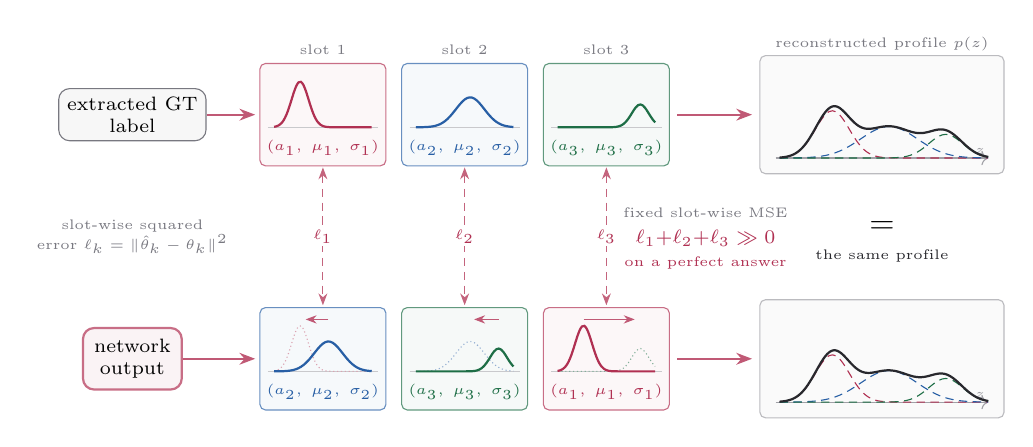
\begin{tikzpicture}
    \foreach \i/\x in {1/0.8,2/2.6,3/4.4}
      \node[font=\tiny,text=soft] at (\x,3.92) {slot \i};
    \node[gate,align=center] (gtl) at (-1.62,3.1) {extracted GT\\ label};
    \node[box]  (hdl) at (-1.62,0) {network\\ output};
    \node[font=\tiny,text=soft,align=center] at (-1.62,1.55) {slot-wise squared\\ error $\ell_k = \lVert\hat\theta_k - \theta_k\rVert^2$};
    \draw[flow] (gtl.east) -- (-0.06,3.1);
    \draw[flow] (hdl.east) -- (-0.06,0);
    \draw[accent!70,thin,rounded corners=2pt,fill=accent!4] (0.0,2.45) rectangle (1.6,3.75);
    \draw[argA!70,thin,rounded corners=2pt,fill=argA!4]     (1.8,2.45) rectangle (3.4,3.75);
    \draw[good!70,thin,rounded corners=2pt,fill=good!4]     (3.6,2.45) rectangle (5.2,3.75);
    \foreach \x in {0.8,2.6,4.4} \draw[soft!40,thin] (\x-0.7,2.94) -- (\x+0.7,2.94);
    \draw[accent,thick,domain=-0.62:0.62,samples=41,smooth,shift={(0.8,2.94)}]
      plot (\x,{0.58*exp(-(\x+0.29)*(\x+0.29)/(2*0.108*0.108))});
    \draw[argA,thick,domain=-0.62:0.62,samples=41,smooth,shift={(2.6,2.94)}]
      plot (\x,{0.38*exp(-(\x-0.07)*(\x-0.07)/(2*0.18*0.18))});
    \draw[good,thick,domain=-0.62:0.62,samples=41,smooth,shift={(4.4,2.94)}]
      plot (\x,{0.29*exp(-(\x-0.43)*(\x-0.43)/(2*0.108*0.108))});
    \node[font=\tiny,text=accent] at (0.8,2.68) {$(a_1,\;\mu_1,\;\sigma_1)$};
    \node[font=\tiny,text=argA]   at (2.6,2.68) {$(a_2,\;\mu_2,\;\sigma_2)$};
    \node[font=\tiny,text=good]   at (4.4,2.68) {$(a_3,\;\mu_3,\;\sigma_3)$};
    \draw[argA!70,thin,rounded corners=2pt,fill=argA!4]     (0.0,-0.65) rectangle (1.6,0.65);
    \draw[good!70,thin,rounded corners=2pt,fill=good!4]     (1.8,-0.65) rectangle (3.4,0.65);
    \draw[accent!70,thin,rounded corners=2pt,fill=accent!4] (3.6,-0.65) rectangle (5.2,0.65);
    \foreach \x in {0.8,2.6,4.4} \draw[soft!40,thin] (\x-0.7,-0.16) -- (\x+0.7,-0.16);
    \draw[accent!45,thin,densely dotted,domain=-0.62:0.62,samples=41,smooth,shift={(0.8,-0.16)}]
      plot (\x,{0.58*exp(-(\x+0.29)*(\x+0.29)/(2*0.108*0.108))});
    \draw[argA,thick,domain=-0.62:0.62,samples=41,smooth,shift={(0.8,-0.16)}]
      plot (\x,{0.38*exp(-(\x-0.07)*(\x-0.07)/(2*0.18*0.18))});
    \draw[argA!50,thin,densely dotted,domain=-0.62:0.62,samples=41,smooth,shift={(2.6,-0.16)}]
      plot (\x,{0.38*exp(-(\x-0.07)*(\x-0.07)/(2*0.18*0.18))});
    \draw[good,thick,domain=-0.62:0.62,samples=41,smooth,shift={(2.6,-0.16)}]
      plot (\x,{0.29*exp(-(\x-0.43)*(\x-0.43)/(2*0.108*0.108))});
    \draw[good!55,thin,densely dotted,domain=-0.62:0.62,samples=41,smooth,shift={(4.4,-0.16)}]
      plot (\x,{0.29*exp(-(\x-0.43)*(\x-0.43)/(2*0.108*0.108))});
    \draw[accent,thick,domain=-0.62:0.62,samples=41,smooth,shift={(4.4,-0.16)}]
      plot (\x,{0.58*exp(-(\x+0.29)*(\x+0.29)/(2*0.108*0.108))});
    \draw[accent!80,thin,-{Stealth[length=1.4mm]}] (0.87,0.50) -- (0.58,0.50);
    \draw[accent!80,thin,-{Stealth[length=1.4mm]}] (3.03,0.50) -- (2.72,0.50);
    \draw[accent!80,thin,-{Stealth[length=1.4mm]}] (4.11,0.50) -- (4.76,0.50);
    \node[font=\tiny,text=argA]   at (0.8,-0.42) {$(a_2,\;\mu_2,\;\sigma_2)$};
    \node[font=\tiny,text=good]   at (2.6,-0.42) {$(a_3,\;\mu_3,\;\sigma_3)$};
    \node[font=\tiny,text=accent] at (4.4,-0.42) {$(a_1,\;\mu_1,\;\sigma_1)$};
    \foreach \x/\e in {0.8/{\ell_1},2.6/{\ell_2},4.4/{\ell_3}} {
      \draw[accent!75,densely dashed,{Stealth[length=1.5mm]}-{Stealth[length=1.5mm]},thin]
        (\x,2.43) -- (\x,0.68);
      \node[font=\tiny,text=accent,fill=white,inner sep=1pt] at (\x,1.55) {$\e$}; }
    \node[font=\tiny,text=soft]         at (5.66,1.85) {fixed slot-wise MSE};
    \node[font=\scriptsize,text=accent] at (5.66,1.53) {$\ell_1{+}\ell_2{+}\ell_3 \gg 0$};
    \node[font=\tiny,text=accent]       at (5.66,1.22) {on a perfect answer};
    \draw[flow] (5.3,3.1) -- (6.25,3.1);
    \draw[flow] (5.3,0.0) -- (6.25,0.0);
    \node[font=\tiny,text=soft] at (7.9,4.00) {reconstructed profile $p(z)$};
    \draw[soft!50,thin,rounded corners=2pt,fill=black!2] (6.35,2.35) rectangle (9.45,3.85);
    \draw[soft!50,thin,rounded corners=2pt,fill=black!2] (6.35,-0.75) rectangle (9.45,0.75);
    \foreach \dy in {2.55,-0.55} {
      \begin{scope}[shift={(6.55,\dy)}]
        \draw[->,soft!70,thin] (0,0) -- (2.70,0) node[above left,font=\tiny,inner sep=1pt]{$z$};
        \draw[accent,thin,densely dashed,domain=0.05:2.7,samples=60,smooth]
          plot (\x,{0.60*exp(-(\x-0.72)*(\x-0.72)/(2*0.216*0.216))});
        \draw[argA,thin,densely dashed,domain=0.05:2.7,samples=60,smooth]
          plot (\x,{0.40*exp(-(\x-1.44)*(\x-1.44)/(2*0.36*0.36))});
        \draw[good,thin,densely dashed,domain=0.05:2.7,samples=60,smooth]
          plot (\x,{0.30*exp(-(\x-2.16)*(\x-2.16)/(2*0.216*0.216))});
        \draw[ink,thick,domain=0.05:2.7,samples=120,smooth]
          plot (\x,{0.60*exp(-(\x-0.72)*(\x-0.72)/(2*0.216*0.216)) + 0.40*exp(-(\x-1.44)*(\x-1.44)/(2*0.36*0.36)) + 0.30*exp(-(\x-2.16)*(\x-2.16)/(2*0.216*0.216))});
      \end{scope} }
    \node[font=\large] at (7.9,1.67) {$=$};
    \node[font=\tiny,text=ink] at (7.9,1.31) {the same profile};
  \end{tikzpicture}
  \end{center}
  \vspace{2pt}
  \centering
  This is the \textbf{permutation-invariance problem} --- the loss must score the
  set, not the slot order.
\end{frame}

% ---------------------------------------------------------------- 13b Sorting instability example
\begin{frame}{The sorting instability, concretely ($K{=}3$)}
  \small
  \begin{columns}[c]
    \begin{column}{0.42\textwidth}
      \footnotesize
      \begin{itemize}
        \setlength{\itemsep}{10pt}
        \item Almost every pixel holds two layers. Under $\mu$-sorting the head
              \emph{specializes}: slot 1 learns the ground, slot 2 learns the canopy,
              and slot 3 almost never sees an active Gaussian --- it learns silence.
        \item A three-layer pixel reshuffles the targets: the volume drops into
              slot 2 --- the canopy specialist --- and the canopy is pushed into
              slot 3 --- the silent slot.
        \item Habits win: slot 2 emits its usual canopy and misses the volume;
              slot 3 stays silent and the canopy loses its predictor --- the rare
              pixel is wrong in every slot at once.
        \item The failure is scoring \emph{slots}; the way out is to score the
              \emph{set} (next).
      \end{itemize}
    \end{column}
    \begin{column}{0.56\textwidth}
      \centering
      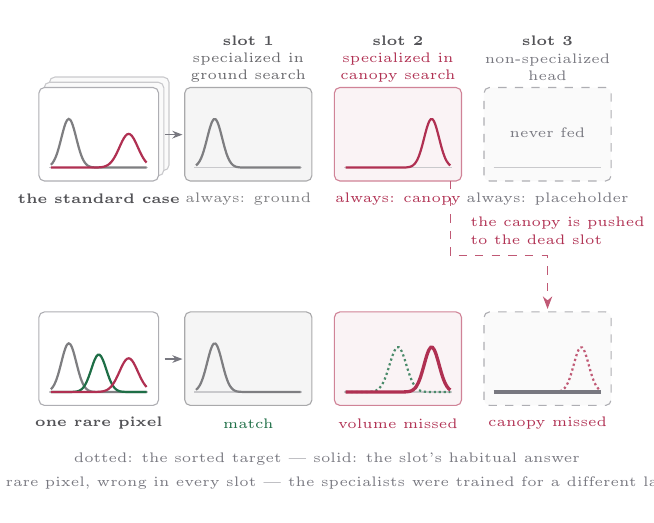
\begin{tikzpicture}[scale=0.95]
    \useasboundingbox (-0.05,0.3) rectangle (7.95,6.55);
    \node[font=\tiny\bfseries,ink!80] at (2.9,6.38) {slot 1};
    \node[font=\tiny\bfseries,ink!80] at (4.9,6.38) {slot 2};
    \node[font=\tiny\bfseries,ink!80] at (6.9,6.38) {slot 3};
    \node[font=\tiny,ink!70,align=center]  at (2.9,6.02) {specialized in\\ground search};
    \node[font=\tiny,accent,align=center]  at (4.9,6.02) {specialized in\\canopy search};
    \node[font=\tiny,soft,align=center]    at (6.9,6.02) {non-specialized\\head};
    % --- row 1: the diet and what each slot learns ---
    \draw[soft!40,thin,rounded corners=2pt,fill=black!2] (0.24,4.64) rectangle (1.84,5.89);
    \draw[soft!40,thin,rounded corners=2pt,fill=black!2] (0.17,4.57) rectangle (1.77,5.82);
    \draw[soft!60,thin,rounded corners=2pt,fill=white]   (0.10,4.50) rectangle (1.70,5.75);
    \draw[soft!40,thin] (0.24,4.68) -- (1.56,4.68);
    \draw[ink!60,thick,domain=0.26:1.54,samples=60,smooth]
      plot (\x,{4.68+0.65*exp(-(\x-0.5)^2/0.02)});
    \draw[accent,thick,domain=0.26:1.54,samples=60,smooth]
      plot (\x,{4.68+0.45*exp(-(\x-1.3)^2/0.03)});
    \node[font=\tiny\bfseries,ink!80] at (0.9,4.26) {the standard case};
    \draw[-{Stealth[length=1.3mm]},soft] (1.78,5.12) -- (2.02,5.12);
    \draw[ink!40,thin,rounded corners=2pt,fill=black!4] (2.05,4.5) rectangle (3.75,5.75);
    \draw[soft!40,thin] (2.18,4.68) -- (3.62,4.68);
    \draw[ink!60,thick,domain=2.2:3.6,samples=60,smooth]
      plot (\x,{4.68+0.65*exp(-(\x-2.45)^2/0.02)});
    \node[font=\tiny,ink!60] at (2.9,4.26) {always: ground};
    \draw[accent!60,thin,rounded corners=2pt,fill=accent!6] (4.05,4.5) rectangle (5.75,5.75);
    \draw[soft!40,thin] (4.18,4.68) -- (5.62,4.68);
    \draw[accent,thick,domain=4.2:5.6,samples=60,smooth]
      plot (\x,{4.68+0.65*exp(-(\x-5.35)^2/0.02)});
    \node[font=\tiny,accent] at (4.9,4.26) {always: canopy};
    \draw[soft!60,thin,dashed,rounded corners=2pt,fill=black!2] (6.05,4.5) rectangle (7.75,5.75);
    \draw[soft!40,thin] (6.18,4.68) -- (7.62,4.68);
    \node[font=\tiny,soft] at (6.9,5.15) {never fed};
    \node[font=\tiny,soft] at (6.9,4.26) {always: placeholder};
    % --- the shove ---
    \draw[accent!80,dashed,-{Stealth[length=1.6mm]}] (5.6,4.5) -- (5.6,3.5) -- (6.9,3.5) -- (6.9,2.79);
    \node[font=\tiny,accent,anchor=west] at (5.74,3.94) {the canopy is pushed};
    \node[font=\tiny,accent,anchor=west] at (5.74,3.72) {to the dead slot};
    % --- row 2: the rare pixel, sorted targets vs habits ---
    \draw[soft!60,thin,rounded corners=2pt,fill=white] (0.10,1.50) rectangle (1.70,2.75);
    \draw[soft!40,thin] (0.24,1.68) -- (1.56,1.68);
    \draw[ink!60,thick,domain=0.26:1.54,samples=60,smooth]
      plot (\x,{1.68+0.65*exp(-(\x-0.5)^2/0.02)});
    \draw[good,thick,domain=0.26:1.54,samples=60,smooth]
      plot (\x,{1.68+0.5*exp(-(\x-0.9)^2/0.02)});
    \draw[accent,thick,domain=0.26:1.54,samples=60,smooth]
      plot (\x,{1.68+0.45*exp(-(\x-1.3)^2/0.03)});
    \node[font=\tiny\bfseries,ink!80] at (0.9,1.26) {one rare pixel};
    \draw[-{Stealth[length=1.3mm]},soft] (1.78,2.12) -- (2.02,2.12);
    \draw[ink!40,thin,rounded corners=2pt,fill=black!4] (2.05,1.50) rectangle (3.75,2.75);
    \draw[soft!40,thin] (2.18,1.68) -- (3.62,1.68);
    \draw[ink!60,thick,domain=2.2:3.6,samples=60,smooth]
      plot (\x,{1.68+0.65*exp(-(\x-2.45)^2/0.02)});
    \node[font=\tiny,good] at (2.9,1.26) {match};
    \draw[accent!60,thin,rounded corners=2pt,fill=accent!6] (4.05,1.50) rectangle (5.75,2.75);
    \draw[soft!40,thin] (4.18,1.68) -- (5.62,1.68);
    \draw[good!80,thick,densely dotted,domain=4.2:5.6,samples=60,smooth]
      plot (\x,{1.68+0.6*exp(-(\x-4.9)^2/0.025)});
    \draw[accent,very thick,domain=4.2:5.6,samples=60,smooth]
      plot (\x,{1.68+0.6*exp(-(\x-5.35)^2/0.02)});
    \node[font=\tiny,accent] at (4.9,1.26) {volume missed};
    \draw[soft!60,thin,dashed,rounded corners=2pt,fill=black!2] (6.05,1.50) rectangle (7.75,2.75);
    \draw[accent!80,thick,densely dotted,domain=6.2:7.6,samples=60,smooth]
      plot (\x,{1.68+0.6*exp(-(\x-7.35)^2/0.02)});
    \draw[soft,very thick] (6.18,1.68) -- (7.62,1.68);
    \node[font=\tiny,accent] at (6.9,1.26) {canopy missed};
    \node[font=\tiny,soft] at (3.95,0.78)
      {dotted: the sorted target --- solid: the slot's habitual answer};
    \node[font=\tiny,soft] at (3.95,0.46)
      {one rare pixel, wrong in every slot --- the specialists were trained for a different label};
      \end{tikzpicture}
    \end{column}
  \end{columns}
\end{frame}

% ---------------------------------------------------------------- 14 Hungarian full slide
\begin{frame}{Hungarian matching}
  \small
  \begin{columns}[c]
    \begin{column}{0.5\textwidth}
      \begin{itemize}
        \item Each Gaussian is a \textbf{point in $(a,\mu,\sigma)$ space}: prediction and
              GT are two point sets; the matcher pairs them by distance and scores the
              \emph{set}, not the slot layout.
      \end{itemize}
      \vspace{6pt}
      \centering
      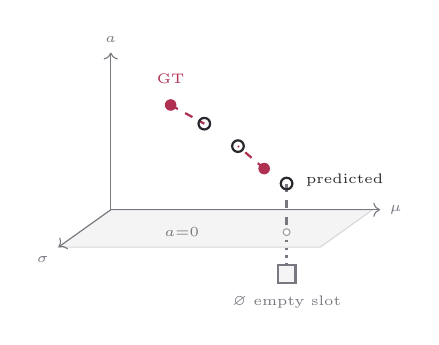
\begin{tikzpicture}[scale=0.95, every node/.style={font=\tiny}]
        \begin{scope}[on background layer]
          \fill[soft!8] (0,0) -- (3.5,0) -- (2.8,-0.5) -- (-0.7,-0.5) -- cycle;
          \draw[soft!30, thin] (0,0) -- (3.5,0) -- (2.8,-0.5) -- (-0.7,-0.5) -- cycle;
        \end{scope}
        \node[soft] at (0.95,-0.30) {$a{=}0$};
        \draw[->,soft] (0,0) -- (3.6,0) node[right]{$\mu$};
        \draw[->,soft] (0,0) -- (0,2.1) node[above]{$a$};
        \draw[->,soft] (0,0) -- (-0.7,-0.5) node[below left]{$\sigma$};
        \draw[accent, dashed, thick] (0.8,1.4) -- (1.25,1.15);
        \draw[accent, dashed, thick] (2.05,0.55) -- (1.7,0.85);
        \draw[soft, dashed, thick] (2.35,0.35) -- (2.35,-0.30);
        \draw[soft, dotted, thick] (2.35,-0.30) -- (2.35,-0.74);
        \fill[accent] (0.8,1.4) circle (2.2pt);
        \fill[accent] (2.05,0.55) circle (2.2pt);
        \draw[ink, thick] (1.25,1.15) circle (2.2pt);
        \draw[ink, thick] (1.7,0.85) circle (2.2pt);
        \draw[ink, thick] (2.35,0.35) circle (2.2pt);
        \draw[soft!70, fill=white] (2.35,-0.30) circle (1.3pt);
        \draw[soft, thick, fill=black!4] (2.23,-0.98) rectangle (2.47,-0.74);
        \node[accent, anchor=south] at (0.8,1.55) {GT};
        \node[ink, anchor=west] at (2.48,0.40) {predicted};
        \node[soft, anchor=north] at (2.35,-1.02) {$\varnothing$ empty slot};
      \end{tikzpicture}
      \\ {\scriptsize Filled = active GT, open = predicted, $\varnothing$ = empty GT slot
      (below $a{=}0$). Its match (grey) is zero-weighted, so $\hat\theta_3$ is free.}
    \end{column}
    \begin{column}{0.5\textwidth}
      \centering
      \[
        \mathcal{L} \;=\; \min_{\pi \in S_K}\ \sum_{k=1}^{K} w_k
          \left\| \hat\theta_{\pi(k)} - \theta_k \right\|^{2}
        \qquad \theta_k = (a_k,\mu_k,\sigma_k)
      \]
      {\scriptsize $w_k=\mathbf{1}[a_k>\tau]$ --- GT \emph{active mask}: $1$ if present, $0$ if empty.}\\[15pt]
      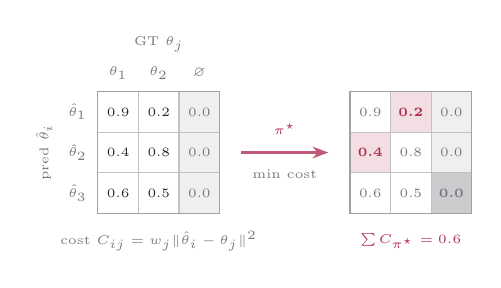
\begin{tikzpicture}[scale=0.92, transform shape, font=\tiny]
        % ===================== cost matrix =====================
        \node[text=soft] at (0.84,0.66) {GT $\theta_j$};
        \node[text=soft] at (0.28,0.26) {$\theta_1$};
        \node[text=soft] at (0.84,0.26) {$\theta_2$};
        \node[text=soft] at (1.40,0.26) {$\varnothing$};
        \node[text=soft, rotate=90] at (-0.74,-0.84) {pred $\hat\theta_i$};
        \node[text=soft] at (-0.28,-0.28) {$\hat\theta_1$};
        \node[text=soft] at (-0.28,-0.84) {$\hat\theta_2$};
        \node[text=soft] at (-0.28,-1.40) {$\hat\theta_3$};
        \fill[soft!12] (1.12,0) rectangle (1.68,-1.68);
        \draw[step=0.56, soft!45, thin] (0,-1.68) grid (1.68,0);
        \draw[soft!70] (0,-1.68) rectangle (1.68,0);
        \node[text=ink]  at (0.28,-0.28) {0.9};
        \node[text=ink]  at (0.84,-0.28) {0.2};
        \node[text=soft] at (1.40,-0.28) {0.0};
        \node[text=ink]  at (0.28,-0.84) {0.4};
        \node[text=ink]  at (0.84,-0.84) {0.8};
        \node[text=soft] at (1.40,-0.84) {0.0};
        \node[text=ink]  at (0.28,-1.40) {0.6};
        \node[text=ink]  at (0.84,-1.40) {0.5};
        \node[text=soft] at (1.40,-1.40) {0.0};
        \node[text=soft] at (0.84,-2.06) {cost $C_{ij}=w_j\lVert\hat\theta_i-\theta_j\rVert^{2}$};
        % ===================== arrow =====================
        \draw[flow] (1.98,-0.84) -- (3.18,-0.84);
        \node[text=accent] at (2.58,-0.52) {$\pi^\star$};
        \node[text=soft]   at (2.58,-1.14) {min cost};
        % ===================== selected matching =====================
        \begin{scope}[shift={(3.48,0)}]
          \fill[soft!12]   (1.12,0)      rectangle (1.68,-1.68);
          \fill[accent!16] (0.56,0)      rectangle (1.12,-0.56);
          \fill[accent!16] (0,-0.56)     rectangle (0.56,-1.12);
          \fill[soft!38]   (1.12,-1.12)  rectangle (1.68,-1.68);
          \draw[step=0.56, soft!45, thin] (0,-1.68) grid (1.68,0);
          \draw[soft!70] (0,-1.68) rectangle (1.68,0);
          \node[text=soft]   at (0.28,-0.28) {0.9};
          \node[text=accent] at (0.84,-0.28) {\textbf{0.2}};
          \node[text=soft]   at (1.40,-0.28) {0.0};
          \node[text=accent] at (0.28,-0.84) {\textbf{0.4}};
          \node[text=soft]   at (0.84,-0.84) {0.8};
          \node[text=soft]   at (1.40,-0.84) {0.0};
          \node[text=soft]   at (0.28,-1.40) {0.6};
          \node[text=soft]   at (0.84,-1.40) {0.5};
          \node[text=soft]   at (1.40,-1.40) {\textbf{0.0}};
          \node[text=accent] at (0.84,-2.06) {$\textstyle\sum C_{\pi^\star}=0.6$};
        \end{scope}
      \end{tikzpicture}\hspace*{2.5em}
      \\[4pt] {\scriptsize Column $\varnothing$ is a placeholder GT ($w_j{=}0$) --- all-zero,
      so the leftover prediction matches it for free:
      $\hat\theta_1\!\to\!\theta_2,\ \hat\theta_2\!\to\!\theta_1,\ \hat\theta_3\!\to\!\varnothing$.}
    \end{column}
  \end{columns}
\end{frame}

% ---------------------------------------------------------------- 15 DETR lineage
\begin{frame}{Set-prediction lineage: DETR}
  \small
  \begin{columns}[c]
    \begin{column}{0.54\textwidth}
      DETR (Carion et al., ECCV 2020) framed detection as \textbf{direct set prediction}:
      bipartite (Hungarian) matching \; + \; a per-element existence mechanism.
      \textbf{The answer to the small-$K$ failure}: grow $K$ until every layer fits, and
      let existence gates close the slots a pixel does not need.
      \vspace{6pt}
      \begin{itemize}
        \item The gate replaces DETR's classification softmax: absence is encoded as
              \emph{zero amplitude}, not a class --- the $3K$-channel contract is
              unchanged.
        \item Under \texttt{sorted\_gt} the gate merely relabels slots ---
              \textbf{pair with Hungarian}.
      \end{itemize}
    \end{column}
    \begin{column}{0.44\textwidth}
      \centering
      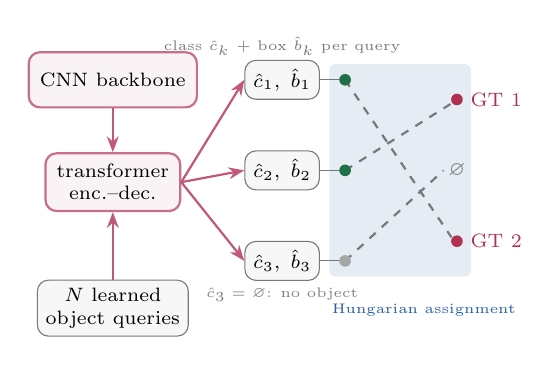
\begin{tikzpicture}[node distance=4mm]
        \node[box, minimum width=15mm] (bb) at (0,1.15)  {CNN backbone};
        \node[box, minimum width=15mm] (tr) at (0,-0.15) {transformer\\enc.--dec.};
        \node[gate]                    (qq) at (0,-1.75) {$N$ learned\\object queries};
        \draw[flow] (bb) -- (tr);
        \draw[flow] (qq) -- (tr);
        \node[gate] (p1) at (2.15,1.15)  {$\hat c_1,\;\hat b_1$};
        \node[gate] (p2) at (2.15,0)     {$\hat c_2,\;\hat b_2$};
        \node[gate] (p3) at (2.15,-1.15) {$\hat c_3,\;\hat b_3$};
        \node[font=\tiny,soft]     at (2.15,1.58)  {class $\hat c_k$ + box $\hat b_k$ per query};
        \node[font=\tiny,black!50] at (2.15,-1.58) {$\hat c_3=\varnothing$: no object};
        \draw[flow] (tr.east) -- (p1.west);
        \draw[flow] (tr.east) -- (p2.west);
        \draw[flow] (tr.east) -- (p3.west);
        \fill[argA!12, rounded corners=2pt] ($(p1.east)+(0.12,0.2)$) rectangle (4.55,-1.35);
        \coordinate (o1) at ($(p1.east)+(0.32,0)$);
        \coordinate (o2) at ($(p2.east)+(0.32,0)$);
        \coordinate (o3) at ($(p3.east)+(0.32,0)$);
        \draw[soft, thin] (p1.east) -- (o1);
        \draw[soft, thin] (p2.east) -- (o2);
        \draw[soft, thin] (p3.east) -- (o3);
        \node[font=\scriptsize,accent] (g1) at (4.87,0.9)  {GT 1};
        \node[font=\scriptsize,accent] (g2) at (4.87,-0.9) {GT 2};
        \node[font=\scriptsize,soft]   (g0) at (4.37,0)    {$\varnothing$};
        \draw[soft, dashed, thick] (o1) -- (4.30,-0.85);
        \draw[soft, dashed, thick] (o2) -- (4.30,0.85);
        \draw[soft, dashed, thick] (o3) -- (4.20,0);
        \fill[good]     (o1) circle (2.1pt);
        \fill[good]     (o2) circle (2.1pt);
        \fill[black!35] (o3) circle (2.1pt);
        \fill[accent] (4.37,0.9)  circle (2.1pt);
        \fill[accent] (4.37,-0.9) circle (2.1pt);
        \node[font=\tiny,argA] at (3.95,-1.78) {Hungarian assignment};
      \end{tikzpicture}
      \\[4pt]
      {\scriptsize DETR: every query emits a class and a box; absence is the explicit
      class $\varnothing$ --- unmatched queries are trained onto $\varnothing$ and
      leave the box loss.}
    \end{column}
  \end{columns}
\end{frame}

% ---------------------------------------------------------------- 15a Set-prediction head mechanism
\begin{frame}{Inside the set-prediction head --- gate, blend, match}
  \small
  \begin{columns}[T]
    \begin{column}{0.56\textwidth}
      \centering
      \vspace{4pt}
      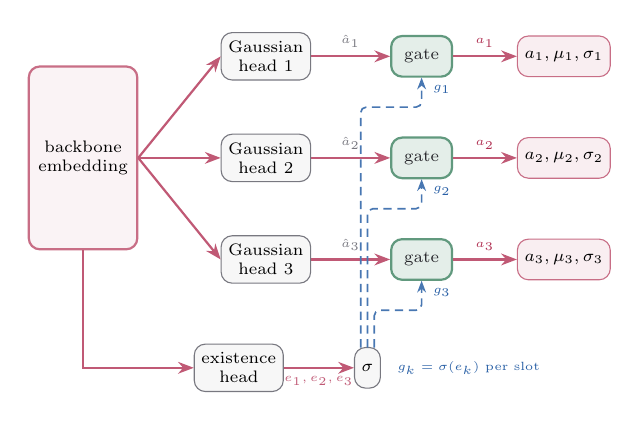
\begin{tikzpicture}[font=\scriptsize, scale=0.86, transform shape,
          exc/.style={-{Stealth[length=1.5mm]}, argA!85, semithick, densely dashed}]
        \node[box, minimum height=27mm, minimum width=16mm] (bb) at (0,0) {backbone\\embedding};
        \node[gate, minimum height=7mm] (h1) at (2.7,1.5)  {Gaussian\\head 1};
        \node[gate, minimum height=7mm] (h2) at (2.7,0)    {Gaussian\\head 2};
        \node[gate, minimum height=7mm] (h3) at (2.7,-1.5) {Gaussian\\head 3};
        \node[box, draw=good!70, fill=good!12, text=ink, minimum height=6mm, minimum width=9mm] (g1) at (5.0,1.5)  {gate};
        \node[box, draw=good!70, fill=good!12, text=ink, minimum height=6mm, minimum width=9mm] (g2) at (5.0,0)    {gate};
        \node[box, draw=good!70, fill=good!12, text=ink, minimum height=6mm, minimum width=9mm] (g3) at (5.0,-1.5) {gate};
        \node[gate, draw=accent!70, fill=accent!8, minimum height=6mm] (o1) at (7.1,1.5)  {$a_1,\mu_1,\sigma_1$};
        \node[gate, draw=accent!70, fill=accent!8, minimum height=6mm] (o2) at (7.1,0)    {$a_2,\mu_2,\sigma_2$};
        \node[gate, draw=accent!70, fill=accent!8, minimum height=6mm] (o3) at (7.1,-1.5) {$a_3,\mu_3,\sigma_3$};
        \node[gate, minimum height=7mm] (eh)  at (2.3,-3.1) {existence\\head};
        \node[gate, minimum height=6mm] (sig) at (4.2,-3.1) {$\sigma$};
        \draw[flow] (bb.east) -- (h1.west);
        \draw[flow] (bb.east) -- (h2.west);
        \draw[flow] (bb.east) -- (h3.west);
        \draw[flow] (bb.south) |- (eh.west);
        \draw[flow] (h1.east) -- node[midway, above, font=\tiny, text=soft]{$\hat a_1$} (g1.west);
        \draw[flow] (h2.east) -- node[midway, above, font=\tiny, text=soft]{$\hat a_2$} (g2.west);
        \draw[flow] (h3.east) -- node[midway, above, font=\tiny, text=soft]{$\hat a_3$} (g3.west);
        \draw[flow] (g1.east) -- node[midway, above, font=\tiny, text=accent]{$a_1$} (o1.west);
        \draw[flow] (g2.east) -- node[midway, above, font=\tiny, text=accent]{$a_2$} (o2.west);
        \draw[flow] (g3.east) -- node[midway, above, font=\tiny, text=accent]{$a_3$} (o3.west);
        \draw[flow] (eh.east) -- (sig.west) node[midway, below, font=\tiny]{$e_1,e_2,e_3$};
        \draw[exc, rounded corners=2pt] (4.10,-2.8) -- (4.10,0.75)  -| (g1.south);
        \draw[exc, rounded corners=2pt] (4.20,-2.8) -- (4.20,-0.75) -| (g2.south);
        \draw[exc, rounded corners=2pt] (4.30,-2.8) -- (4.30,-2.25) -| (g3.south);
        \node[font=\tiny, text=argA, anchor=north] at (5.3,1.2)  {$g_1$};
        \node[font=\tiny, text=argA, anchor=north] at (5.3,-0.3) {$g_2$};
        \node[font=\tiny, text=argA, anchor=north] at (5.3,-1.8) {$g_3$};
        \node[font=\tiny, text=argA, anchor=west] at ($(sig.east)+(0.12,0)$) {$g_k=\sigma(e_k)$ per slot};
      \end{tikzpicture}
      \\[8pt]
      {\footnotesize each gate:\; $a_k = g_k\,\hat a_k + (1-g_k)\,a_{\mathrm{off},k}$}\\[1pt]
      {\scriptsize\color{soft} $\mu_k,\sigma_k$ pass through $\cdot$ $a_{\mathrm{off}}$ learned per slot}
    \end{column}
    \begin{column}{0.44\textwidth}
      \footnotesize
      \textbf{The gate is a sigmoid} on the existence logit $e_k$:
      \begin{itemize}\setlength{\itemsep}{5pt}
        \item Open slots ($g_k\!\to\!1$): $a_k \approx \hat a_k$ --- the raw regression survives.
        \item Closed slot ($g_k\!\to\!0$): $a_k \to a_{\mathrm{off},k}\approx 0$ \emph{whatever}
              $\hat a_k$ is, collapsing onto the empty-set target at near-zero loss.
        \item $e_k$ is internal --- the head still emits $3K$ channels $(a_k,\mu_k,\sigma_k)$;
              $a_{\mathrm{off}}$ is a learned per-slot scalar (init $0$).
      \end{itemize}
      \vspace{8pt}
      \centering
      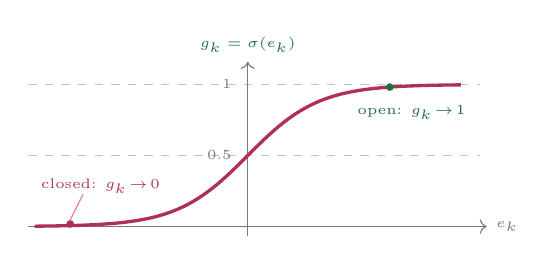
\begin{tikzpicture}[scale=0.82, font=\scriptsize]
        \draw[soft!45, dashed] (-3.4,2.2) -- (3.6,2.2);
        \draw[soft!45, dashed] (-3.4,1.1) -- (3.6,1.1);
        \node[soft, font=\tiny, anchor=east] at (-0.1,2.2) {1};
        \node[soft, font=\tiny, anchor=east] at (-0.1,1.1) {0.5};
        \draw[->, soft] (-3.4,0) -- (3.7,0) node[right, font=\tiny]{$e_k$};
        \draw[->, soft] (0,-0.15) -- (0,2.55) node[above, font=\tiny, text=good]{$g_k=\sigma(e_k)$};
        \draw[accent, very thick, samples=90, domain=-6:6] plot ({\x*0.55},{2.2/(1+exp(-\x))});
        \fill[good] (2.2,2.16) circle (1.7pt);
        \node[good, font=\tiny, anchor=north west] at (1.55,2.02) {open: $g_k\!\to\!1$};
        \fill[accent] (-2.75,0.04) circle (1.7pt);
        \node[accent, font=\tiny, anchor=west] at (-3.35,0.62) {closed: $g_k\!\to\!0$};
        \draw[accent!60, thin] (-2.75,0.1) -- (-2.55,0.5);
      \end{tikzpicture}
    \end{column}
  \end{columns}
\end{frame}

% ---------------------------------------------------------------- 15b Hungarian 2x2
\begin{frame}{Set prediction, controlled --- the head is the lever, not the matching}
    \centering
  \scriptsize
  \renewcommand{\arraystretch}{1.1}
  \setlength{\tabcolsep}{5pt}
  \renewcommand{\seedtag}{setA}
  \begin{tabular}{@{}l cc !{\hspace{3pt}} cc@{}}
    \toprule
     & \multicolumn{2}{c}{conv head} & \multicolumn{2}{c@{}}{set-pred head} \\
    \cmidrule(lr){2-3}\cmidrule(l){4-5}
    metric & sort & Hung & sort & Hung \\
    \midrule
    \multicolumn{5}{@{}l}{\emph{reconstruction (curve)}} \\
    curve $R^2$ $\uparrow$  & \seedpm{0.569}{.008} & \seedpm{\textbf{0.603}}{.012} & \seedpm{0.536}{.026} & \seedpm{0.578}{.016} \\
    curve MAE $\downarrow$  & \seedpm{0.0496}{.0008} & \seedpm{\textbf{0.0471}}{.0005} & \seedpm{0.0503}{.0016} & \seedpm{0.0480}{.0011} \\
    PSNR [dB] $\uparrow$    & \seedpm{50.3}{.1} & \seedpm{50.7}{.1} & \seedpm{50.0}{.2} & \seedpm{50.4}{.2} \\
    SSIM elev $\uparrow$    & \seedpm{0.9586}{.0006} & \seedpm{0.9601}{.0003} & \seedpm{0.9586}{.0010} & \seedpm{0.9598}{.0009} \\
    SSIM range $\uparrow$   & \seedpm{0.9258}{.0021} & \seedpm{0.9277}{.0019} & \seedpm{0.9329}{.0039} & \seedpm{0.9342}{.0028} \\
    SSIM azim $\uparrow$    & \seedpm{0.9461}{.0012} & \seedpm{0.9479}{.0007} & \seedpm{0.9471}{.0020} & \seedpm{0.9488}{.0014} \\
    profile cos med $\uparrow$ & \seedpm{0.850}{.024} & \seedpm{0.854}{.022} & \seedpm{\textbf{0.904}}{.034} & \seedpm{0.896}{.033} \\
    \addlinespace
    \multicolumn{5}{@{}l}{\emph{detection (matched)}} \\
    peak err mean $\downarrow$ & \seedpm{4.70}{.47} & \seedpm{4.80}{.52} & \seedpm{1.66}{.09} & \seedpm{\hlval{good}{\textbf{1.63}}}{.08} \\
    \quad median $\downarrow$  & \seedpm{0.81}{.30} & \seedpm{1.07}{.37} & \seedpm{\textbf{0.67}}{.00} & \seedpm{\textbf{0.67}}{.00} \\
    \quad p95 $\downarrow$     & \seedpm{15.44}{.47} & \seedpm{15.57}{.56} & \seedpm{6.71}{.47} & \seedpm{\hlval{good}{\textbf{6.04}}}{.47} \\
    precision $\uparrow$   & \seedpm{0.821}{.008} & \seedpm{0.822}{.002} & \seedpm{0.816}{.005} & \seedpm{0.813}{.004} \\
    recall $\uparrow$      & \seedpm{0.641}{.029} & \seedpm{0.642}{.045} & \seedpm{0.887}{.008} & \seedpm{\hlval{good}{\textbf{0.893}}}{.004} \\
    matched F1 $\uparrow$  & \seedpm{0.720}{.020} & \seedpm{0.720}{.027} & \seedpm{0.850}{.006} & \seedpm{\textbf{0.851}}{.004} \\
    count exact $\uparrow$ & \seedpm{0.595}{.034} & \seedpm{0.590}{.044} & \seedpm{\hlval{good}{\textbf{0.852}}}{.004} & \seedpm{0.841}{.004} \\
    \quad under $\downarrow$ & \seedpm{0.327}{.036} & \seedpm{0.329}{.057} & \seedpm{0.018}{.005} & \seedpm{\hlval{good}{\textbf{0.017}}}{.004} \\
    \quad over $\downarrow$  & \seedpm{\textbf{0.078}}{.004} & \seedpm{0.081}{.012} & \seedpm{\hlval{accent}{0.130}}{.005} & \seedpm{\hlval{accent}{0.143}}{.003} \\
    \bottomrule
  \end{tabular}
  \par\vspace{3pt}
  \parbox{0.82\textwidth}{\tiny\color{soft} \textbf{runs}: UNet $\cdot$ $K{=}2$ $\cdot$ param-MSE $\cdot$ presence none $\cdot$ full norm ladder $\cdot$ hv flips $\cdot$ patch $64{\times}32$ (head $\times$ matching $=$ 2$\times$2); five seeded replicas per arm, cells mean $\pm$ seed std; held-out test. \textbf{bold} $=$ best in row, marked only where best and worst differ by more than $5\%$; \textcolor{good}{green} $=$ the gate's detection lift; \textcolor{accent}{red} $=$ its over-count price. Peak median/p95: per-pixel peak-error distribution; profile cos med: median per-pixel cosine to the GT profile.\par}
    

\end{frame}

% ---------------------------------------------------------------- 15c Head 2x2 by scatterer count
\begin{frame}{The head by scatterer count --- the gate saturates $k{=}1$, layover pays}
    \centering
  \scriptsize
  \renewcommand{\arraystretch}{1.05}
  \setlength{\tabcolsep}{5pt}
  \renewcommand{\seedtag}{setB}
  \begin{tabular}{@{}l cc !{\hspace{3pt}} cc@{}}
    \toprule
     & \multicolumn{2}{c}{conv head} & \multicolumn{2}{c@{}}{set-pred head} \\
    \cmidrule(lr){2-3}\cmidrule(l){4-5}
    metric & sort & Hung & sort & Hung \\
    \midrule
    matched precision $\uparrow$ & \seedpm{0.821}{.008} & \seedpm{0.822}{.002} & \seedpm{0.816}{.005} & \seedpm{0.813}{.004} \\
    \quad $k{=}1$                & \seedpm{0.853}{.008} & \seedpm{0.848}{.004} & \seedpm{0.849}{.005} & \seedpm{0.836}{.003} \\
    \quad $k{=}2$                & \seedpm{0.782}{.007} & \seedpm{0.790}{.002} & \seedpm{0.759}{.014} & \seedpm{0.771}{.009} \\
    \addlinespace
    matched recall $\uparrow$    & \seedpm{0.641}{.029} & \seedpm{0.642}{.045} & \seedpm{0.887}{.008} & \seedpm{\textbf{0.893}}{.004} \\
    \quad $k{=}1$                & \seedpm{0.620}{.046} & \seedpm{0.617}{.071} & \seedpm{\hlval{good}{\textbf{0.997}}}{.001} & \seedpm{\hlval{good}{\textbf{0.997}}}{.000} \\
    \quad $k{=}2$                & \seedpm{0.672}{.008} & \seedpm{0.677}{.007} & \seedpm{0.731}{.019} & \seedpm{\textbf{0.744}}{.010} \\
    \addlinespace
    count acc $\mid$ pred $k{=}1$ $\uparrow$ & \seedpm{0.948}{.007} & \seedpm{0.951}{.013} & \seedpm{0.975}{.006} & \seedpm{0.977}{.004} \\
    count acc $\mid$ pred $k{=}2$ $\uparrow$ & \seedpm{\textbf{0.733}}{.010} & \seedpm{0.725}{.026} & \seedpm{0.651}{.007} & \seedpm{\hlval{accent}{0.631}}{.005} \\
    \addlinespace
    matched $\mu$ MAE $\downarrow$ & \seedpm{2.30}{.08} & \seedpm{2.29}{.10} & \seedpm{\textbf{2.18}}{.09} & \seedpm{2.19}{.08} \\
    \quad $k{=}1$                & \seedpm{0.59}{.04} & \seedpm{\textbf{0.56}}{.05} & \seedpm{0.59}{.10} & \seedpm{0.62}{.11} \\
    \quad $k{=}2$                & \seedpm{\textbf{4.05}}{.08} & \seedpm{4.06}{.02} & \seedpm{\hlval{accent}{4.54}}{.11} & \seedpm{4.51}{.13} \\
    \addlinespace
    matched $\sigma$ MAE $\downarrow$ & \seedpm{0.87}{.03} & \seedpm{0.87}{.04} & \seedpm{\textbf{0.82}}{.03} & \seedpm{0.83}{.03} \\
    \quad $k{=}1$                & \seedpm{0.25}{.01} & \seedpm{0.26}{.02} & \seedpm{\textbf{0.23}}{.01} & \seedpm{0.24}{.01} \\
    \quad $k{=}2$                & \seedpm{1.51}{.01} & \seedpm{\textbf{1.50}}{.01} & \seedpm{1.70}{.06} & \seedpm{\hlval{accent}{1.71}}{.06} \\
    \addlinespace
    matched $a$ MAE $\downarrow$ & \seedpm{0.374}{.026} & \seedpm{0.380}{.033} & \seedpm{\textbf{0.306}}{.002} & \seedpm{0.311}{.004} \\
    \quad $k{=}1$                & \seedpm{0.161}{.017} & \seedpm{0.180}{.026} & \seedpm{\hlval{good}{\textbf{0.114}}}{.004} & \seedpm{0.133}{.005} \\
    \quad $k{=}2$                & \seedpm{0.593}{.022} & \seedpm{0.585}{.023} & \seedpm{0.590}{.006} & \seedpm{0.573}{.011} \\
    \bottomrule
  \end{tabular}
  \par\vspace{3pt}
  \parbox{0.82\textwidth}{\tiny\color{soft} \textbf{runs}: UNet $\cdot$ $K{=}2$ $\cdot$ param-MSE $\cdot$ presence none $\cdot$ full norm ladder $\cdot$ hv flips $\cdot$ patch $64{\times}32$ (head $\times$ matching = column); held-out test, cells mean $\pm$ seed std over five seeded replicas; $k$ $=$ true scatterer count of the pixel. \textbf{bold} $=$ best in row, marked only where best and worst differ by more than $5\%$; \textcolor{good}{green} $=$ the gate's $k{=}1$ saturation and amplitude win, \textcolor{accent}{red} $=$ the layover price. Precision rewards under-prediction --- rank on recall. count acc $\mid$ pred $k$: share of pixels claiming exactly $k$ scatterers whose true count is $k$. $\mu$, $\sigma$ in elevation units; $a$ in linear amplitude.\par}
    

\end{frame}

% ---------------------------------------------------------------- 15d Head 2x2: predicted stats vs GT
\begin{frame}{The head, predicted statistics vs the GT --- the gate calibrates activity, pays in amplitude}
    \centering
  \scriptsize
  \renewcommand{\arraystretch}{0.95}
  \setlength{\tabcolsep}{5pt}
  \renewcommand{\seedtag}{setC}
  \begin{tabular}{@{}l !{\color{white}\vrule width 2pt} c !{\color{white}\vrule width 2pt} cc !{\hspace{3pt}} cc@{}}
    \toprule
    & & \multicolumn{2}{c}{conv head} & \multicolumn{2}{c@{}}{set-pred head} \\
    \cmidrule(lr){3-4}\cmidrule(l){5-6}
    prediction mean & \textcolor{good}{GT} & sort & Hung & sort & Hung \\
    \midrule
    \multicolumn{6}{@{}l}{\textcolor{soft}{\emph{slot 0 --- strongest scatterer; GT-active on every pixel}}} \\
    \quad active frac         & 1.00    & \seedpm{0.69}{.03} & \seedpm{0.68}{.05} & \seedpm{\hlval{good}{\textbf{0.990}}}{.003} & \seedpm{\hlval{good}{\textbf{0.990}}}{.002} \\
    \addlinespace[2pt]
    \quad $a$ --- active      & 0.77    & \seedpm{0.90}{.03} & \seedpm{\textbf{0.87}}{.05} & \seedpm{\hlval{accent}{0.61}}{.01} & \seedpm{\hlval{accent}{0.58}}{.01} \\
    \quad $\mu$ --- active    & $-4.89$ & \seedpm{$-3.92$}{.10} & \seedpm{$-3.66$}{.13} & \seedpm{\textbf{$-4.38$}}{.22} & \seedpm{$-4.13$}{.14} \\
    \quad $\sigma$ --- active & 1.76    & \seedpm{1.48}{.05} & \seedpm{\textbf{1.50}}{.07} & \seedpm{1.34}{.03} & \seedpm{1.38}{.03} \\
    \addlinespace
    \multicolumn{6}{@{}l}{\textcolor{soft}{\emph{slot 1 --- second scatterer; GT-active on 26\% of pixels}}} \\
    \quad active frac         & 0.260 & \seedpm{\textbf{0.299}}{.006} & \seedpm{0.304}{.015} & \seedpm{\hlval{accent}{0.380}}{.008} & \seedpm{\hlval{accent}{0.394}}{.005} \\
    \addlinespace[2pt]
    \quad $a$ --- active      & 1.43  & \seedpm{1.04}{.03} & \seedpm{\textbf{1.10}}{.02} & \seedpm{0.89}{.02} & \seedpm{0.94}{.03} \\
    \addlinespace[2pt]
    \quad $a$ --- inact.      & 0.00  & \seedpm{0.42}{.01} & \seedpm{0.52}{.07} & \seedpm{\hlval{good}{\textbf{0.30}}}{.02} & \seedpm{0.39}{.04} \\
    \quad $\mu$ --- active    & 11.34 & \seedpm{\textbf{10.09}}{.33} & \seedpm{9.15}{.26} & \seedpm{9.77}{.50} & \seedpm{8.80}{.32} \\
    \quad $\mu$ --- inact.    & ---   & \seedpm{4.09}{.31} & \seedpm{2.04}{.75} & \seedpm{2.57}{.37} & \seedpm{$-0.29$}{.37} \\
    \quad $\sigma$ --- active & 3.53  & \seedpm{2.94}{.05} & \seedpm{\textbf{2.98}}{.06} & \seedpm{2.80}{.08} & \seedpm{2.78}{.05} \\
    \quad $\sigma$ --- inact. & ---   & \seedpm{1.87}{.03} & \seedpm{1.76}{.05} & \seedpm{1.76}{.03} & \seedpm{1.70}{.03} \\
    \addlinespace
    \multicolumn{6}{@{}l}{\textcolor{soft}{\emph{distribution width --- std over GT-active pixels}}} \\
    \quad $a$ --- slot 0      & 1.48  & \seedpm{\textbf{1.17}}{.03} & \seedpm{1.16}{.03} & \seedpm{0.91}{.01} & \seedpm{0.93}{.03} \\
    \quad $\mu$ --- slot 0    & 3.30  & \seedpm{1.99}{.07} & \seedpm{2.13}{.11} & \seedpm{2.00}{.08} & \seedpm{\textbf{2.23}}{.16} \\
    \quad $\sigma$ --- slot 0 & 2.84  & \seedpm{0.95}{.03} & \seedpm{1.03}{.04} & \seedpm{0.93}{.03} & \seedpm{\textbf{1.07}}{.03} \\
    \quad $a$ --- slot 1      & 1.45  & \seedpm{0.83}{.04} & \seedpm{\textbf{0.91}}{.02} & \seedpm{0.77}{.03} & \seedpm{0.82}{.03} \\
    \quad $\mu$ --- slot 1    & 16.24 & \seedpm{8.72}{.18} & \seedpm{8.88}{.13} & \seedpm{8.86}{.74} & \seedpm{\textbf{9.47}}{.21} \\
    \quad $\sigma$ --- slot 1 & 4.01  & \seedpm{1.07}{.02} & \seedpm{\textbf{1.24}}{.05} & \seedpm{1.04}{.05} & \seedpm{1.15}{.05} \\
    \bottomrule
  \end{tabular}
  \par\vspace{3pt}
  \parbox{0.82\textwidth}{\tiny\color{soft} \textbf{runs}: UNet $\cdot$ $K{=}2$ $\cdot$ param-MSE $\cdot$ presence none $\cdot$ full norm ladder $\cdot$ hv flips $\cdot$ patch $64{\times}32$ (head $\times$ matching = column); five seeded replicas per arm, cells mean $\pm$ seed std; means conditioned on the slot's GT activity mask. \textbf{bold} $=$ closest to the \textcolor{good}{GT} column, marked only where best and worst differ by more than $5\%$; \textcolor{good}{green} $=$ the gate's activity and leakage wins, \textcolor{accent}{red} $=$ the slot-1 over-fire and the amplitude payment. Inactive GT slots define no $\mu$/$\sigma$ reference (---). Width rows: std of the prediction over GT-active pixels vs the GT's own std. $\mu$, $\sigma$ in elevation units; $a$ in linear amplitude.\par}
    

\end{frame}

% ---------------------------------------------------------------- 15e Head 2x2 at K=5
\begin{frame}{Set prediction at $K{=}5$ --- the head still leads, and the matching now matters}
    \centering
  \scriptsize
  \renewcommand{\arraystretch}{1.1}
  \setlength{\tabcolsep}{5pt}
  \renewcommand{\seedtag}{khA}
  \begin{tabular}{@{}l cc !{\hspace{3pt}} cc@{}}
    \toprule
     & \multicolumn{2}{c}{conv head} & \multicolumn{2}{c@{}}{set-pred head} \\
    \cmidrule(lr){2-3}\cmidrule(l){4-5}
    metric & sort & Hung & sort & Hung \\
    \midrule
    \multicolumn{5}{@{}l}{\emph{reconstruction (curve)}} \\
    curve $R^2$ $\uparrow$ & \seedpm{0.561}{.019} & \seedpm{\textbf{0.587}}{.012} & \seedpm{0.534}{.007} & \seedpm{0.566}{.016} \\
    curve MAE $\downarrow$ & \seedpm{0.0554}{.0006} & \seedpm{\textbf{0.0521}}{.0005} & \seedpm{0.0565}{.0007} & \seedpm{0.0537}{.0008} \\
    PSNR [dB] $\uparrow$ & \seedpm{49.7}{.2} & \seedpm{49.9}{.1} & \seedpm{49.4}{.1} & \seedpm{49.7}{.2} \\
    SSIM elev $\uparrow$ & \seedpm{0.9530}{.0007} & \seedpm{0.9565}{.0005} & \seedpm{0.9527}{.0014} & \seedpm{0.9553}{.0020} \\
    SSIM range $\uparrow$ & \seedpm{0.9234}{.0028} & \seedpm{0.9319}{.0039} & \seedpm{0.9296}{.0020} & \seedpm{0.9314}{.0026} \\
    SSIM azim $\uparrow$ & \seedpm{0.9435}{.0011} & \seedpm{0.9475}{.0011} & \seedpm{0.9439}{.0013} & \seedpm{0.9466}{.0016} \\
    profile cos med $\uparrow$ & \seedpm{0.838}{.041} & \seedpm{0.895}{.028} & \seedpm{\textbf{0.905}}{.012} & \seedpm{0.891}{.014} \\
    \addlinespace
    \multicolumn{5}{@{}l}{\emph{detection (matched)}} \\
    peak err mean $\downarrow$ & \seedpm{4.83}{.71} & \seedpm{2.58}{1.51} & \seedpm{1.64}{.04} & \seedpm{\hlval{good}{\textbf{1.56}}}{.10} \\
    \quad median $\downarrow$ & \seedpm{0.81}{.30} & \seedpm{\textbf{0.67}}{.00} & \seedpm{\textbf{0.67}}{.00} & \seedpm{\textbf{0.67}}{.00} \\
    \quad p95 $\downarrow$ & \seedpm{15.44}{.47} & \seedpm{9.93}{4.26} & \seedpm{7.38}{.00} & \seedpm{\hlval{good}{\textbf{5.77}}}{.37} \\
    precision $\uparrow$ & \seedpm{0.620}{.011} & \seedpm{\textbf{0.636}}{.038} & \seedpm{0.627}{.009} & \seedpm{0.573}{.027} \\
    recall $\uparrow$ & \seedpm{\hlval{accent}{0.648}}{.040} & \seedpm{0.802}{.093} & \seedpm{0.867}{.006} & \seedpm{\hlval{good}{\textbf{0.886}}}{.003} \\
    matched F1 $\uparrow$ & \seedpm{0.633}{.025} & \seedpm{0.709}{.058} & \seedpm{\textbf{0.728}}{.007} & \seedpm{0.696}{.020} \\
    count exact $\uparrow$ & \seedpm{0.430}{.050} & \seedpm{0.574}{.131} & \seedpm{\textbf{0.651}}{.004} & \seedpm{0.588}{.062} \\
    \quad under $\downarrow$ & \seedpm{0.320}{.055} & \seedpm{0.134}{.122} & \seedpm{0.031}{.002} & \seedpm{\hlval{good}{\textbf{0.027}}}{.004} \\
    \quad over $\downarrow$ & \seedpm{\textbf{0.251}}{.008} & \seedpm{0.292}{.021} & \seedpm{0.318}{.006} & \seedpm{\hlval{accent}{0.385}}{.065} \\
    \bottomrule
  \end{tabular}
  \par\vspace{3pt}
  \parbox{0.82\textwidth}{\tiny\color{soft} \textbf{runs}: UNet $\cdot$ $K{=}5$ $\cdot$ param-MSE $\cdot$ presence none $\cdot$ full norm ladder $\cdot$ hv flips $\cdot$ patch $64{\times}32$ (head $\times$ matching $=$ 2$\times$2); five seeded replicas per arm, cells mean $\pm$ seed std; held-out test. \textbf{bold} $=$ best in row, marked only where best and worst differ by more than $5\%$; \textcolor{good}{green} $=$ the gate's detection lift; \textcolor{accent}{red} $=$ the over-count price and the sorted-GT break. Peak median/p95: per-pixel peak-error distribution; profile cos med: median per-pixel cosine to the GT profile.\par}
    

\end{frame}

% ---------------------------------------------------------------- 15f Head 2x2 at K=5 by scatterer count
\begin{frame}{The $K{=}5$ head by scatterer count --- the gate saturates $k{=}1$, recall fades up the ladder}
    \centering
  \scriptsize
  \renewcommand{\arraystretch}{1.0}
  \setlength{\tabcolsep}{5pt}
  \renewcommand{\seedtag}{khB}
  \begin{tabular}{@{}l cc !{\hspace{3pt}} cc@{}}
    \toprule
     & \multicolumn{2}{c}{conv head} & \multicolumn{2}{c@{}}{set-pred head} \\
    \cmidrule(lr){2-3}\cmidrule(l){4-5}
    metric & sort & Hung & sort & Hung \\
    \midrule
    matched precision $\uparrow$ & \seedpm{0.620}{.011} & \seedpm{\textbf{0.636}}{.038} & \seedpm{0.627}{.009} & \seedpm{0.573}{.027} \\
    \quad $k{=}1$ & \seedpm{0.711}{.018} & \seedpm{0.719}{.057} & \seedpm{\textbf{0.726}}{.008} & \seedpm{0.640}{.045} \\
    \quad $k{=}2$ & \seedpm{\textbf{0.562}}{.011} & \seedpm{0.535}{.020} & \seedpm{0.525}{.009} & \seedpm{0.471}{.015} \\
    \quad $k{=}3$ & \seedpm{0.549}{.009} & \seedpm{\textbf{0.574}}{.010} & \seedpm{0.519}{.016} & \seedpm{0.538}{.009} \\
    \quad $k{=}4$ & \seedpm{0.421}{.002} & \seedpm{\textbf{0.525}}{.007} & \seedpm{0.419}{.014} & \seedpm{0.510}{.011} \\
    \quad $k{=}5$ & \seedpm{0.393}{.014} & \seedpm{\textbf{0.470}}{.013} & \seedpm{0.394}{.010} & \seedpm{0.468}{.011} \\
    \addlinespace
    matched recall $\uparrow$ & \seedpm{0.648}{.040} & \seedpm{0.802}{.093} & \seedpm{0.867}{.006} & \seedpm{\textbf{0.886}}{.003} \\
    \quad $k{=}1$ & \seedpm{0.643}{.070} & \seedpm{0.876}{.162} & \seedpm{\hlval{good}{\textbf{0.996}}}{.002} & \seedpm{0.994}{.002} \\
    \quad $k{=}2$ & \seedpm{0.830}{.010} & \seedpm{0.862}{.011} & \seedpm{0.893}{.008} & \seedpm{\textbf{0.906}}{.009} \\
    \quad $k{=}3$ & \seedpm{0.645}{.005} & \seedpm{0.718}{.010} & \seedpm{0.684}{.017} & \seedpm{\hlval{good}{\textbf{0.763}}}{.004} \\
    \quad $k{=}4$ & \seedpm{0.375}{.008} & \seedpm{0.489}{.010} & \seedpm{0.421}{.015} & \seedpm{\textbf{0.527}}{.010} \\
    \quad $k{=}5$ & \seedpm{0.233}{.003} & \seedpm{0.290}{.016} & \seedpm{0.281}{.010} & \seedpm{\textbf{0.327}}{.015} \\
    \addlinespace
    \multicolumn{5}{@{}l}{\emph{count acc $\mid$ pred $k$ $\uparrow$ --- share of pixels claiming exactly $k$ whose true count is $k$}} \\
    \quad pred $k{=}1$ & \seedpm{0.948}{.010} & \seedpm{0.965}{.011} & \seedpm{0.973}{.005} & \seedpm{0.978}{.008} \\
    \addlinespace[2pt]
    \quad pred $k{=}2$ & \seedpm{\textbf{0.315}}{.016} & \seedpm{0.262}{.039} & \seedpm{0.251}{.006} & \seedpm{\hlval{accent}{0.173}}{.061} \\
    \quad pred $k{=}3$ & \seedpm{\textbf{0.124}}{.008} & \seedpm{0.100}{.018} & \seedpm{0.095}{.008} & \seedpm{0.050}{.011} \\
    \quad pred $k{=}4$ & \seedpm{\textbf{0.072}}{.006} & \seedpm{0.051}{.011} & \seedpm{0.047}{.005} & \seedpm{0.024}{.006} \\
    \quad pred $k{=}5$ & \seedpm{\textbf{0.102}}{.012} & \seedpm{0.081}{.004} & \seedpm{0.075}{.005} & \seedpm{0.063}{.009} \\
    \bottomrule
  \end{tabular}
  \par\vspace{3pt}
  \parbox{0.82\textwidth}{\tiny\color{soft} \textbf{runs}: UNet $\cdot$ $K{=}5$ $\cdot$ param-MSE $\cdot$ presence none $\cdot$ full norm ladder $\cdot$ hv flips $\cdot$ patch $64{\times}32$ (head $\times$ matching $=$ 2$\times$2); five seeded replicas per arm, cells mean $\pm$ seed std; held-out test. \textbf{bold} $=$ best in row, marked only where best and worst differ by more than $5\%$; $k$ $=$ true scatterer count of the pixel. \textcolor{good}{green} $=$ the $k{=}1$ saturation and the higher-rung wins; \textcolor{accent}{red} $=$ the unreliable claimed pairs. Precision rewards under-prediction --- read it alongside recall. count acc $\mid$ pred $k$: share of pixels claiming exactly $k$ scatterers whose true count is $k$.\par}
    

\end{frame}

% ---------------------------------------------------------------- 15g Head 2x2 at K=5: component errors
\begin{frame}{The $K{=}5$ components --- position pays for the crowd, the sorted arms keep the widths}
    \centering
  \scriptsize
  \renewcommand{\arraystretch}{1.0}
  \setlength{\tabcolsep}{5pt}
  \renewcommand{\seedtag}{khC}
  \begin{tabular}{@{}l cc !{\hspace{3pt}} cc@{}}
    \toprule
     & \multicolumn{2}{c}{conv head} & \multicolumn{2}{c@{}}{set-pred head} \\
    \cmidrule(lr){2-3}\cmidrule(l){4-5}
    metric & sort & Hung & sort & Hung \\
    \midrule
    matched $\mu$ MAE $\downarrow$ & \seedpm{2.30}{.14} & \seedpm{\textbf{1.90}}{.12} & \seedpm{2.05}{.06} & \seedpm{1.94}{.06} \\
    \quad $k{=}1$ & \seedpm{0.69}{.09} & \seedpm{\textbf{0.63}}{.04} & \seedpm{0.65}{.05} & \seedpm{0.75}{.08} \\
    \quad $k{=}2$ & \seedpm{\textbf{1.81}}{.04} & \seedpm{1.83}{.09} & \seedpm{1.99}{.05} & \seedpm{1.83}{.09} \\
    \quad $k{=}3$ & \seedpm{4.24}{.10} & \seedpm{3.63}{.16} & \seedpm{4.32}{.11} & \seedpm{\textbf{3.60}}{.14} \\
    \quad $k{=}4$ & \seedpm{7.88}{.20} & \seedpm{\hlval{good}{\textbf{6.48}}}{.13} & \seedpm{7.50}{.23} & \seedpm{6.55}{.25} \\
    \quad $k{=}5$ & \seedpm{9.56}{.28} & \seedpm{9.16}{.23} & \seedpm{9.43}{.18} & \seedpm{9.48}{.26} \\
    \addlinespace
    matched $\sigma$ MAE $\downarrow$ & \seedpm{0.79}{.04} & \seedpm{0.79}{.05} & \seedpm{\hlval{good}{\textbf{0.70}}}{.01} & \seedpm{0.77}{.03} \\
    \quad $k{=}1$ & \seedpm{0.35}{.03} & \seedpm{0.36}{.04} & \seedpm{\textbf{0.29}}{.01} & \seedpm{0.35}{.03} \\
    \quad $k{=}2$ & \seedpm{\textbf{0.97}}{.01} & \seedpm{1.11}{.04} & \seedpm{1.00}{.00} & \seedpm{1.12}{.04} \\
    \quad $k{=}3$ & \seedpm{\textbf{1.36}}{.01} & \seedpm{1.45}{.05} & \seedpm{1.41}{.01} & \seedpm{1.46}{.03} \\
    \quad $k{=}4$ & \seedpm{\textbf{1.60}}{.01} & \seedpm{1.70}{.08} & \seedpm{1.70}{.00} & \seedpm{1.70}{.04} \\
    \quad $k{=}5$ & \seedpm{\textbf{1.66}}{.01} & \seedpm{1.84}{.13} & \seedpm{1.83}{.01} & \seedpm{1.81}{.07} \\
    \addlinespace
    matched $a$ MAE $\downarrow$ & \seedpm{0.526}{.026} & \seedpm{0.564}{.050} & \seedpm{\hlval{good}{\textbf{0.442}}}{.008} & \seedpm{0.552}{.044} \\
    \quad $k{=}1$ & \seedpm{0.172}{.015} & \seedpm{0.230}{.040} & \seedpm{\textbf{0.130}}{.007} & \seedpm{0.235}{.058} \\
    \quad $k{=}2$ & \seedpm{\textbf{0.725}}{.023} & \seedpm{0.906}{.053} & \seedpm{0.744}{.014} & \seedpm{\hlval{accent}{0.920}}{.048} \\
    \quad $k{=}3$ & \seedpm{\textbf{1.018}}{.020} & \seedpm{1.091}{.016} & \seedpm{1.024}{.013} & \seedpm{1.096}{.030} \\
    \quad $k{=}4$ & \seedpm{1.067}{.015} & \seedpm{1.078}{.026} & \seedpm{1.038}{.011} & \seedpm{1.049}{.026} \\
    \quad $k{=}5$ & \seedpm{0.988}{.015} & \seedpm{1.001}{.041} & \seedpm{\textbf{0.895}}{.007} & \seedpm{0.915}{.041} \\
    \bottomrule
  \end{tabular}
  \par\vspace{3pt}
  \parbox{0.82\textwidth}{\tiny\color{soft} \textbf{runs}: UNet $\cdot$ $K{=}5$ $\cdot$ param-MSE $\cdot$ presence none $\cdot$ full norm ladder $\cdot$ hv flips $\cdot$ patch $64{\times}32$ (head $\times$ matching $=$ 2$\times$2); five seeded replicas per arm, cells mean $\pm$ seed std; held-out test. \textbf{bold} $=$ best in row, marked only where best and worst differ by more than $5\%$; $k$ $=$ true scatterer count of the pixel; component errors over matched pairs only. \textcolor{good}{green} $=$ the Hungarian $\mu$ buy and the sorted-arm component wins; \textcolor{accent}{red} $=$ the amplitude Hungarian pays. $\mu$, $\sigma$ in elevation units; $a$ in linear amplitude.\par}
    

\end{frame}

% ---------------------------------------------------------------- 15h Head 2x2 at K=5: predicted stats vs GT
\begin{frame}{The $K{=}5$ head, predicted statistics vs the GT --- slot 0 calibrated, the tail over-fired}
    \centering
  \scriptsize
  \renewcommand{\arraystretch}{0.85}
  \setlength{\tabcolsep}{5pt}
  \renewcommand{\seedtag}{khD}
  \begin{tabular}{@{}l !{\color{white}\vrule width 2pt} c !{\color{white}\vrule width 2pt} cc !{\hspace{3pt}} cc@{}}
    \toprule
    & & \multicolumn{2}{c}{conv head} & \multicolumn{2}{c@{}}{set-pred head} \\
    \cmidrule(lr){3-4}\cmidrule(l){5-6}
    prediction mean & \textcolor{good}{GT} & sort & Hung & sort & Hung \\
    \midrule
    \multicolumn{6}{@{}l}{\textcolor{soft}{\emph{predicted active fraction --- share of pixels where the slot fires}}} \\
    \quad slot 0 & 1.000 & \seedpm{0.701}{.054} & \seedpm{0.880}{.126} & \seedpm{\hlval{good}{\textbf{0.989}}}{.002} & \seedpm{0.983}{.004} \\
    \quad slot 1 & 0.239 & \seedpm{0.319}{.009} & \seedpm{\textbf{0.278}}{.050} & \seedpm{0.385}{.005} & \seedpm{0.324}{.042} \\
    \quad slot 2 & 0.085 & \seedpm{0.218}{.006} & \seedpm{\textbf{0.193}}{.065} & \seedpm{0.263}{.003} & \seedpm{0.234}{.046} \\
    \quad slot 3 & 0.035 & \seedpm{\textbf{0.137}}{.005} & \seedpm{0.169}{.050} & \seedpm{0.162}{.013} & \seedpm{\hlval{accent}{0.239}}{.056} \\
    \quad slot 4 & 0.015 & \seedpm{\textbf{0.060}}{.015} & \seedpm{0.207}{.068} & \seedpm{0.099}{.009} & \seedpm{\hlval{accent}{0.349}}{.087} \\
    \addlinespace
    \multicolumn{6}{@{}l}{\textcolor{soft}{\emph{$a$ --- predicted mean over GT-active pixels}}} \\
    \quad slot 0 & 0.84 & \seedpm{\textbf{0.99}}{.08} & \seedpm{0.64}{.14} & \seedpm{0.67}{.01} & \seedpm{0.51}{.06} \\
    \quad slot 1 & 1.67 & \seedpm{\textbf{0.94}}{.04} & \seedpm{0.67}{.07} & \seedpm{0.80}{.02} & \seedpm{0.67}{.05} \\
    \quad slot 2 & 1.41 & \seedpm{0.30}{.02} & \seedpm{\textbf{0.71}}{.07} & \seedpm{0.26}{.02} & \seedpm{0.57}{.05} \\
    \quad slot 3 & 0.97 & \seedpm{0.14}{.01} & \seedpm{\textbf{0.28}}{.05} & \seedpm{0.12}{.01} & \seedpm{0.23}{.02} \\
    \quad slot 4 & 0.66 & \seedpm{0.09}{.01} & \seedpm{\textbf{0.21}}{.01} & \seedpm{0.07}{.01} & \seedpm{0.19}{.03} \\
    \addlinespace
    \multicolumn{6}{@{}l}{\textcolor{soft}{\emph{$a$ --- predicted mean over GT-inactive pixels (leakage)}}} \\
    \quad slot 1 & 0.00 & \seedpm{0.65}{.02} & \seedpm{\textbf{0.26}}{.21} & \seedpm{0.46}{.01} & \seedpm{0.39}{.21} \\
    \quad slot 2 & 0.00 & \seedpm{0.37}{.01} & \seedpm{0.40}{.18} & \seedpm{\textbf{0.29}}{.00} & \seedpm{0.40}{.12} \\
    \quad slot 3 & 0.00 & \seedpm{0.17}{.01} & \seedpm{0.56}{.25} & \seedpm{\textbf{0.14}}{.00} & \seedpm{0.31}{.20} \\
    \quad slot 4 & 0.00 & \seedpm{0.11}{.01} & \seedpm{0.58}{.39} & \seedpm{\textbf{0.07}}{.01} & \seedpm{0.41}{.31} \\
    \addlinespace
    \multicolumn{6}{@{}l}{\textcolor{soft}{\emph{distribution width --- std over GT-active pixels}}} \\
    \quad $a$ --- slot 0 & 1.59 & \seedpm{\textbf{1.33}}{.07} & \seedpm{1.09}{.09} & \seedpm{1.04}{.02} & \seedpm{0.92}{.04} \\
    \quad $\mu$ --- slot 0 & 3.02 & \seedpm{\textbf{2.47}}{.06} & \seedpm{2.37}{.05} & \seedpm{2.28}{.04} & \seedpm{2.39}{.12} \\
    \quad $\sigma$ --- slot 0 & 1.72 & \seedpm{0.80}{.02} & \seedpm{0.71}{.11} & \seedpm{0.79}{.04} & \seedpm{\textbf{0.86}}{.10} \\
    \quad $a$ --- slot 1 & 1.60 & \seedpm{0.82}{.02} & \seedpm{\textbf{0.87}}{.05} & \seedpm{0.75}{.01} & \seedpm{0.83}{.02} \\
    \quad $\mu$ --- slot 1 & 11.09 & \seedpm{8.44}{.10} & \seedpm{8.83}{.10} & \seedpm{8.48}{.10} & \seedpm{\textbf{8.98}}{.15} \\
    \quad $\sigma$ --- slot 1 & 2.30 & \seedpm{0.87}{.02} & \seedpm{1.28}{.03} & \seedpm{0.88}{.01} & \seedpm{\textbf{1.29}}{.04} \\
    \bottomrule
  \end{tabular}
  \par\vspace{1pt}
  \parbox{0.82\textwidth}{\tiny\color{soft} \textbf{runs}: UNet $\cdot$ $K{=}5$ $\cdot$ param-MSE $\cdot$ presence none $\cdot$ full norm ladder $\cdot$ hv flips $\cdot$ patch $64{\times}32$ (head $\times$ matching $=$ 2$\times$2); five seeded replicas per arm, cells mean $\pm$ seed std; held-out test; means conditioned on the slot's GT activity mask. \textbf{bold} $=$ closest to the \textcolor{good}{GT} column, marked only where best and worst differ by more than $5\%$; \textcolor{good}{green} $=$ the calibrated slot-0 gate, \textcolor{accent}{red} $=$ the over-fired tail slots. Width rows: std of the prediction over GT-active pixels vs the GT's own std, shown for slots 0--1 (tail slots in the report). $\mu$, $\sigma$ in elevation units; $a$ in linear amplitude.\par}
    

\end{frame}

% ---------------------------------------------------------------- 16 Imbalance & collapse
\begin{frame}{The imbalance failure (high $K$)}
  \small
  \setlength{\abovedisplayskip}{4pt}
  \setlength{\belowdisplayskip}{4pt}
  \begin{columns}[c]
    \begin{column}{0.42\textwidth}
      \footnotesize
      \begin{itemize}
        \setlength{\itemsep}{10pt}
        \item Hungarian + existence gates make large $K$ trainable --- and expose the
              third failure: \textbf{most slots have nothing to match}.
        \item The matcher hands slot $k$ a real scatterer (amplitude $a^{+}$) in a
              fraction $\rho_k$ of cells, silence in the rest --- deep slots see
              $\rho_k\approx0.01$. Mean-reduced, the slot's amplitude minimizes the
              two-point mixture on the right (param-MSE).
        \item The push outweighs the pull $99{:}1$; descent parks the slot at $1\%$
              of the real amplitude --- \textbf{shrinking to effective silence is
              the loss optimum}, not a training accident.
        \item The working $K{=}2$ configuration mostly sidesteps the tail; the $K{=}5$
              development confronts it head-on --- the answer (next).
      \end{itemize}
    \end{column}
    \begin{column}{0.56\textwidth}
      \centering
      {\footnotesize
      \begin{align*}
        \ell_k(\hat a)
          &= \big(\hat a - a^{\text{match}}_k\big)^{2},
             \qquad
             a^{\text{match}}_k \;=\;
             \begin{cases}
               a^{+} & \text{with prob.\ } \rho_k \\
               0     & \text{with prob.\ } 1-\rho_k
             \end{cases} \\[3pt]
        \mathrm E\big[\ell_k(\hat a)\big]
          &= \rho_k\, \mathrm E\big[(\hat a - a^{+})^2\big] \;+\; (1-\rho_k)\,\hat a^{2} \\[3pt]
        \partial_{\hat a}\,\mathrm E\big[\ell_k\big]
          &= \underbrace{2\rho_k\,\big(\hat a - \mathrm E[a^{+}]\big)}_{\text{\scriptsize pull toward the target}}
             \;+\; \underbrace{2\,(1-\rho_k)\,\hat a}_{\text{\scriptsize push toward silence}} \\[3pt]
          &= 2\,\big(\hat a - \rho_k\,\mathrm E[a^{+}]\big)
             \;\Longrightarrow\;
             \hat a^{*}_k \;=\; \rho_k\,\mathrm E[a^{+}] \;\approx\; 0.01\,\mathrm E[a^{+}]
      \end{align*}}
      \vspace{2pt}

      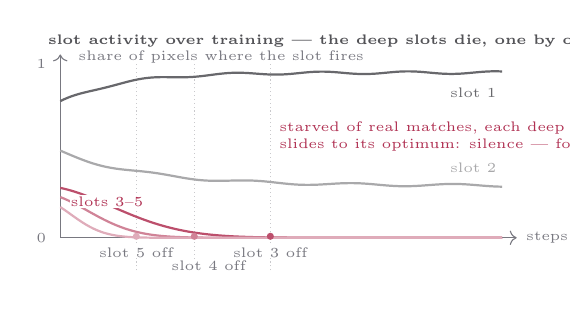
\begin{tikzpicture}[scale=0.92]
    \useasboundingbox (-0.15,1.35) rectangle (6.95,4.85);
    % --- death moments ---
    \draw[soft!40,densely dotted] (1.35,1.50) -- (1.35,4.35);
    \draw[soft!40,densely dotted] (2.15,1.50) -- (2.15,4.35);
    \draw[soft!40,densely dotted] (3.20,1.50) -- (3.20,4.35);
    % --- slot activity over training ---
    \node[font=\tiny\bfseries,ink!80,anchor=west] at (0,4.66)
      {slot activity over training --- the deep slots die, one by one};
    \draw[->,soft] (0.3,1.95) -- (0.3,4.48);
    \node[font=\tiny,soft,anchor=east] at (0.24,4.35) {1};
    \node[font=\tiny,soft,anchor=east] at (0.24,1.95) {0};
    \node[font=\tiny,soft,anchor=west] at (0.42,4.44) {share of pixels where the slot fires};
    \draw[->,soft] (0.3,1.95) -- (6.6,1.95) node[right,font=\tiny]{steps};
    \draw[ink!70,thick,domain=0.3:6.4,samples=120,smooth]
      plot (\x,{4.23-0.60*exp(-\x/0.8)+0.018*sin(300*\x)});
    \draw[ink!40,thick,domain=0.3:6.4,samples=120,smooth]
      plot (\x,{2.67+0.60*exp(-\x/1.2)+0.018*sin(260*\x+40)});
    \draw[accent!85,thick,domain=0.3:6.4,samples=120,smooth]
      plot (\x,{1.95+0.72*exp(-\x*\x/2.0)});
    \draw[accent!60,thick,domain=0.3:6.4,samples=120,smooth]
      plot (\x,{1.95+0.62*exp(-\x*\x/0.9)});
    \draw[accent!40,thick,domain=0.3:6.4,samples=120,smooth]
      plot (\x,{1.95+0.53*exp(-\x*\x/0.4)});
    \fill[accent!85] (3.20,1.97) circle (1.4pt);
    \fill[accent!60] (2.15,1.97) circle (1.4pt);
    \fill[accent!40] (1.35,1.97) circle (1.4pt);
    \node[font=\tiny,ink!70,anchor=west] at (5.55,3.95) {slot 1};
    \node[font=\tiny,ink!40,anchor=west] at (5.55,2.92) {slot 2};
    \node[font=\tiny,accent,anchor=west,fill=white,inner sep=0.5pt] at (0.42,2.45) {slots 3--5};
    \node[font=\tiny,accent,anchor=west,align=left,fill=white,inner sep=0.5pt] at (3.30,3.35)
      {starved of real matches, each deep slot\\
       slides to its optimum: silence --- for good};
    \node[font=\tiny,soft,fill=white,inner sep=0.5pt] at (1.35,1.75) {slot 5 off};
    \node[font=\tiny,soft,fill=white,inner sep=0.5pt] at (2.35,1.57) {slot 4 off};
    \node[font=\tiny,soft,fill=white,inner sep=0.5pt] at (3.20,1.75) {slot 3 off};
      \end{tikzpicture}
    \end{column}
  \end{columns}
\end{frame}

% ---------------------------------------------------------------- 17a Active normalization
\begin{frame}{The answer to slot imbalance --- lever 1: active normalization}
  \begin{columns}[c]
    \begin{column}{0.40\textwidth}
      \footnotesize
      \emph{Active} slot $=$ the GT placed a real scatterer in it:
      \[
        m_{p,k} \;=\; \mathbf{1}\big[\,a^{\text{GT}}_{p,k} > \tau\,\big]
      \]
      \vspace{-8pt}
      \begin{center}
      {\scriptsize\color{soft} pixel $p$, slot $k$; $\tau = 10^{-3}$ linear
       amplitude --- empty slots carry $a{=}0$. A \emph{pixel} is active when
       any of its $K$ slots is.}
      \end{center}
      \vspace{18pt}
      The lever --- one reduction, dividing by the \textbf{weight mass}, not
      the cell count:
      \[
        \ell \;=\; \frac{\sum_{p,k} w_{p,k}\, e_{p,k}}{\sum_{p,k} w_{p,k}}
      \]
      \vspace{-8pt}
      \begin{center}
      {\scriptsize\color{soft} $e$ = matched error; $w$ per term: $a$ everywhere,
       $\mu,\sigma$ masked by $m$ --- nothing to tune.}
      \end{center}
\end{column}
    \begin{column}{0.58\textwidth}
      \centering
      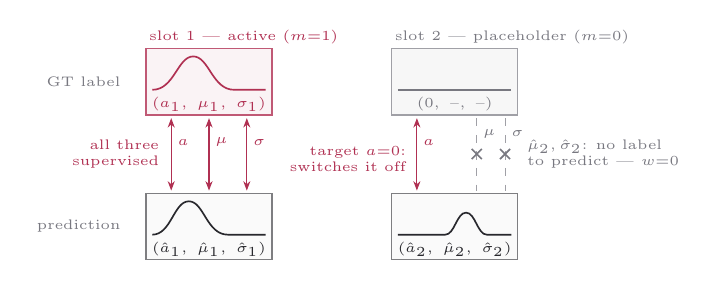
\begin{tikzpicture}[scale=0.80, font=\tiny]

        \node[text=soft, anchor=east] at (-0.25,4.58) {GT label};
        \node[text=accent, anchor=south west, inner sep=1pt] at (0,5.12) {slot 1 --- active ($m{=}1$)};
        \draw[accent!80, thin, fill=accent!6] (0,4.05) rectangle ++(2.0,1.05);
        \draw[accent, semithick] (0.10,4.45)
          .. controls (0.45,4.45) and (0.50,4.98) .. (0.75,4.98)
          .. controls (1.00,4.98) and (1.05,4.45) .. (1.40,4.45) -- (1.90,4.45);
        \node[text=accent] at (1.00,4.22) {$(a_1,\ \mu_1,\ \sigma_1)$};
        \node[text=soft, anchor=south west, inner sep=1pt] at (3.9,5.12) {slot 2 --- placeholder ($m{=}0$)};
        \draw[soft!70, thin, fill=black!3] (3.9,4.05) rectangle ++(2.0,1.05);
        \draw[soft, semithick] (4.00,4.45) -- (5.80,4.45);
        \node[text=soft] at (4.90,4.22) {$(0,\ \text{--},\ \text{--})$};

        \node[text=soft, anchor=east] at (-0.25,2.28) {prediction};
        \draw[ink!60, thin, fill=black!2] (0,1.75) rectangle ++(2.0,1.05);
        \draw[ink, semithick] (0.10,2.15)
          .. controls (0.40,2.15) and (0.44,2.68) .. (0.68,2.68)
          .. controls (0.92,2.68) and (0.96,2.15) .. (1.30,2.15) -- (1.90,2.15);
        \node[text=ink] at (1.00,1.92) {$(\hat a_1,\ \hat\mu_1,\ \hat\sigma_1)$};
        \draw[ink!60, thin, fill=black!2] (3.9,1.75) rectangle ++(2.0,1.05);
        \draw[ink, semithick] (4.00,2.15) -- (4.75,2.15)
          .. controls (4.90,2.15) and (4.93,2.50) .. (5.08,2.50)
          .. controls (5.23,2.50) and (5.26,2.15) .. (5.41,2.15) -- (5.80,2.15);
        \node[text=ink] at (4.90,1.92) {$(\hat a_2,\ \hat\mu_2,\ \hat\sigma_2)$};

        \draw[{Stealth[length=1.2mm]}-{Stealth[length=1.2mm]}, accent, thin] (0.40,4.00) -- (0.40,2.85);
        \draw[{Stealth[length=1.2mm]}-{Stealth[length=1.2mm]}, accent, thin] (1.00,4.00) -- (1.00,2.85);
        \draw[{Stealth[length=1.2mm]}-{Stealth[length=1.2mm]}, accent, thin] (1.60,4.00) -- (1.60,2.85);
        \node[text=accent, anchor=west, inner sep=1.5pt] at (0.43,3.62) {$a$};
        \node[text=accent, anchor=west, inner sep=1.5pt] at (1.03,3.62) {$\mu$};
        \node[text=accent, anchor=west, inner sep=1.5pt] at (1.63,3.62) {$\sigma$};
        \node[text=accent, anchor=east, align=right, inner sep=1.5pt] at (0.28,3.43) {all three\\supervised};

        \draw[{Stealth[length=1.2mm]}-{Stealth[length=1.2mm]}, accent, thin] (4.30,4.00) -- (4.30,2.85);
        \node[text=accent, anchor=west, inner sep=1.5pt] at (4.33,3.62) {$a$};
        \node[text=accent, anchor=east, align=right, inner sep=1.5pt] at (4.20,3.35) {target $a{=}0$:\\switches it off};
        \draw[soft!70, dashed, thin] (5.25,4.00) -- (5.25,2.85);
        \draw[soft!70, dashed, thin] (5.70,4.00) -- (5.70,2.85);
        \node[text=soft, anchor=west, inner sep=1.5pt] at (5.28,3.75) {$\mu$};
        \node[text=soft, anchor=west, inner sep=1.5pt] at (5.73,3.75) {$\sigma$};
        \draw[soft, semithick] (5.17,3.35) -- (5.33,3.51);
        \draw[soft, semithick] (5.17,3.51) -- (5.33,3.35);
        \draw[soft, semithick] (5.62,3.35) -- (5.78,3.51);
        \draw[soft, semithick] (5.62,3.51) -- (5.78,3.35);
        \node[text=soft, anchor=west, align=left, inner sep=1.5pt] at (5.98,3.43) {$\hat\mu_2, \hat\sigma_2$: no label\\to predict --- $w{=}0$};
      \end{tikzpicture}
      \\[2pt]
      {\footnotesize
      \begin{align*}
        \ell_a      &= \frac{\sum_{p,k} \bigl(\hat a - a^{\text{GT}}\bigr)^{2}}{N_{\text{pix}}\,K} \\[-1pt]
        \ell_\mu    &= \frac{\sum_{p,k} m\,\bigl(\hat\mu - \mu^{\text{GT}}\bigr)^{2}}{N_{\text{pix}}\,K}
          \;\to\;
          \frac{\sum_{p,k} m\,\bigl(\hat\mu - \mu^{\text{GT}}\bigr)^{2}}{\denomhl{\sum_{p,k} m}} \\[-1pt]
        \ell_\sigma &= \frac{\sum_{p,k} m\,\bigl(\hat\sigma - \sigma^{\text{GT}}\bigr)^{2}}{N_{\text{pix}}\,K}
          \;\to\;
          \frac{\sum_{p,k} m\,\bigl(\hat\sigma - \sigma^{\text{GT}}\bigr)^{2}}{\denomhl{\sum_{p,k} m}}
      \end{align*}}
    \end{column}
  \end{columns}
\end{frame}

% ---------------------------------------------------------------- 17b Presence balance
\begin{frame}{The answer to slot imbalance --- lever 2: presence balance}
  \setlength{\abovedisplayskip}{3pt}
  \setlength{\belowdisplayskip}{3pt}
  \begin{columns}[c]
    \begin{column}{0.44\textwidth}
      \footnotesize
      \begin{itemize}\setlength{\itemsep}{6pt}
        \item \textbf{The imbalance is per slot}: sorting stacks the scatterers
              early --- slot 1 nearly always active, the tail nearly never; one
              batch-wide fraction cannot see the tail.
        \item \textbf{Presence balance --- inverse class frequency, slot by
              slot}: within every slot actives and empties carry half each:
      \end{itemize}
      \begin{align*}
        w_{p,k} &= \frac{0.5}{f_k}\; m_{p,k} \;+\; \frac{0.5}{1-f_k}\;\big(1 - m_{p,k}\big) \\[2pt]
        f_k     &= \operatorname{clip}\!\big(\langle m_{p,k} \rangle_p,\; \varepsilon,\; 1-\varepsilon\big)
      \end{align*}
      \vspace{-8pt}
      \begin{center}
      {\scriptsize\color{soft} $m$ as on lever 1; $f_k$ measured per batch
       ($\approx \rho_k$), clipped at $\varepsilon = 10^{-3}$.\par}
      \end{center}
    \end{column}
    \begin{column}{0.54\textwidth}
      \centering
      {\footnotesize
      \begin{align*}
        \mathrm E\big[w\,\ell_k\big]
          &= f_k\tfrac{0.5}{f_k}\,\mathrm E\big[(\hat a{-}a^{+})^2\big] + (1{-}f_k)\tfrac{0.5}{1-f_k}\,\hat a^{2} \\[1pt]
          &= \tfrac{1}{2}\,\mathrm E\big[(\hat a - a^{+})^2\big] \;+\; \tfrac{1}{2}\,\hat a^{2}
      \end{align*}
      \vspace{-2pt}
      \begin{align*}
        \partial_{\hat a}\,\mathrm E\big[w\,\ell_k\big]
          &= \hat a - \mathrm E[a^{+}] \;+\; \hat a \\[1pt]
        \hat a^{*}_k &:\;\; \rho_k\,\mathrm E[a^{+}] \;\to\; \textcolor{accent}{\tfrac{1}{2}}\,\mathrm E[a^{+}]
      \end{align*}}

      \vspace{15pt}

      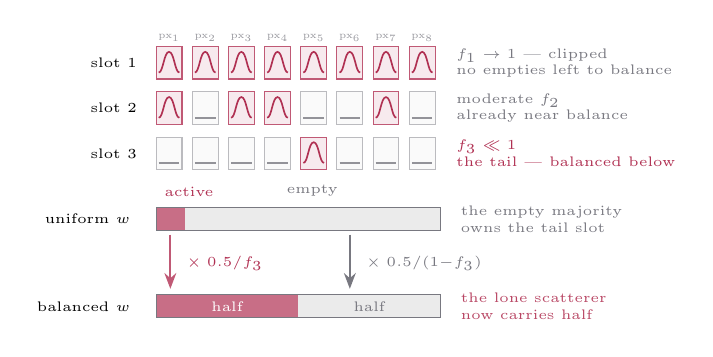
\begin{tikzpicture}[scale=0.82]
        \foreach \i [evaluate=\i as \j using {int(\i+1)}] in {0,...,7}
          \node[font=\tiny, scale=0.7, text=soft!75] at (\i*0.56+0.20,6.74) {$\mathrm{px}_{\j}$};

        \node[font=\tiny, anchor=east] at (-0.15,6.35) {slot 1};
        \foreach \i in {0,...,7} {
          \draw[accent!80, thin, fill=accent!10] (\i*0.56,6.10) rectangle ++(0.40,0.50);
          \draw[accent, semithick] (\i*0.56+0.04,6.20)
            .. controls (\i*0.56+0.11,6.20) and (\i*0.56+0.12,6.52) .. (\i*0.56+0.20,6.52)
            .. controls (\i*0.56+0.28,6.52) and (\i*0.56+0.29,6.20) .. (\i*0.56+0.36,6.20);
        }
        \node[font=\tiny, text=soft, anchor=west, align=left] at (4.50,6.35)
          {$f_1 \to 1$ --- clipped\\no empties left to balance};

        \node[font=\tiny, anchor=east] at (-0.15,5.65) {slot 2};
        \foreach \i in {0,2,3,6} {
          \draw[accent!80, thin, fill=accent!10] (\i*0.56,5.40) rectangle ++(0.40,0.50);
          \draw[accent, semithick] (\i*0.56+0.04,5.50)
            .. controls (\i*0.56+0.11,5.50) and (\i*0.56+0.12,5.82) .. (\i*0.56+0.20,5.82)
            .. controls (\i*0.56+0.28,5.82) and (\i*0.56+0.29,5.50) .. (\i*0.56+0.36,5.50);
        }
        \foreach \i in {1,4,5,7} {
          \draw[soft!50, thin, fill=black!2] (\i*0.56,5.40) rectangle ++(0.40,0.50);
          \draw[soft!80, semithick] (\i*0.56+0.04,5.50) -- (\i*0.56+0.36,5.50);
        }
        \node[font=\tiny, text=soft, anchor=west, align=left] at (4.50,5.65)
          {moderate $f_2$\\already near balance};

        \node[font=\tiny, anchor=east] at (-0.15,4.95) {slot 3};
        \foreach \i in {4} {
          \draw[accent!80, thin, fill=accent!10] (\i*0.56,4.70) rectangle ++(0.40,0.50);
          \draw[accent, semithick] (\i*0.56+0.04,4.80)
            .. controls (\i*0.56+0.11,4.80) and (\i*0.56+0.12,5.12) .. (\i*0.56+0.20,5.12)
            .. controls (\i*0.56+0.28,5.12) and (\i*0.56+0.29,4.80) .. (\i*0.56+0.36,4.80);
        }
        \foreach \i in {0,1,2,3,5,6,7} {
          \draw[soft!50, thin, fill=black!2] (\i*0.56,4.70) rectangle ++(0.40,0.50);
          \draw[soft!80, semithick] (\i*0.56+0.04,4.80) -- (\i*0.56+0.36,4.80);
        }
        \node[font=\tiny, text=accent, anchor=west, align=left] at (4.50,4.95)
          {$f_3 \ll 1$\\the tail --- balanced below};


        \node[font=\tiny, text=accent, anchor=south west] at (-0.02,4.13) {active};
        \node[font=\tiny, text=soft, anchor=south] at (2.42,4.13) {empty};
        \node[font=\tiny, anchor=east] at (-0.25,3.93) {uniform $w$};
        \fill[accent!70] (0,3.75)    rectangle (0.44,4.11);
        \fill[black!8]   (0.44,3.75) rectangle (4.4,4.11);
        \draw[soft, thin] (0,3.75)   rectangle (4.4,4.11);
        \node[font=\tiny, text=soft, anchor=west, align=left] at (4.57,3.93)
          {the empty majority\\owns the tail slot};

        \draw[flow] (0.22,3.69) -- (0.22,2.85);
        \node[font=\tiny, text=accent, anchor=west] at (0.32,3.25) {$\times\;0.5/f_3$};
        \draw[-{Stealth[length=2mm]}, soft, thick] (3.00,3.69) -- (3.00,2.85);
        \node[font=\tiny, text=soft, anchor=west] at (3.10,3.25) {$\times\;0.5/(1{-}f_3)$};

        \node[font=\tiny, anchor=east] at (-0.25,2.58) {balanced $w$};
        \fill[accent!70] (0,2.40)   rectangle (2.2,2.76);
        \fill[black!8]   (2.2,2.40) rectangle (4.4,2.76);
        \draw[soft, thin] (0,2.40)  rectangle (4.4,2.76);
        \node[font=\tiny, text=white] at (1.10,2.58) {half};
        \node[font=\tiny, text=soft]  at (3.30,2.58) {half};
        \node[font=\tiny, text=accent!90, anchor=west, align=left] at (4.57,2.58)
          {the lone scatterer\\now carries half};

      \end{tikzpicture}
    \end{column}
  \end{columns}
\end{frame}

% ---------------------------------------------------------------- 18 Two levers re-measured
\begin{frame}{The two levers, re-measured under Hungarian matching --- A stays free, B now costs recall}
    \centering
  \scriptsize
  \renewcommand{\arraystretch}{0.86}
  \setlength{\tabcolsep}{6pt}
  \renewcommand{\seedtag}{setD}
  \begin{tabular}{@{}l c c c c@{}}
    \toprule
    metric & none & $+$A & $+$B & $+$AB \\
    \midrule
    \multicolumn{5}{@{}l}{\emph{reconstruction (curve)}} \\
    curve $R^2$ $\uparrow$  & \seedpm{0.578}{.016} & \seedpm{0.579}{.017} & \seedpm{0.553}{.011} & \seedpm{0.558}{.014} \\
    curve MAE $\downarrow$  & \seedpm{0.0480}{.0011} & \seedpm{0.0479}{.0008} & \seedpm{0.0493}{.0008} & \seedpm{0.0489}{.0007} \\
    PSNR [dB] $\uparrow$    & \seedpm{50.41}{.17} & \seedpm{50.43}{.17} & \seedpm{50.16}{.11} & \seedpm{50.21}{.14} \\
    SSIM elev $\uparrow$    & \seedpm{0.9598}{.0009} & \seedpm{0.9600}{.0007} & \seedpm{0.9589}{.0007} & \seedpm{0.9592}{.0006} \\
    SSIM range $\uparrow$   & \seedpm{0.9342}{.0028} & \seedpm{0.9346}{.0025} & \seedpm{0.9308}{.0027} & \seedpm{0.9319}{.0018} \\
    SSIM azim $\uparrow$    & \seedpm{0.9488}{.0014} & \seedpm{0.9491}{.0011} & \seedpm{0.9466}{.0011} & \seedpm{0.9471}{.0008} \\
    profile cos med $\uparrow$ & \seedpm{0.896}{.033} & \seedpm{0.892}{.042} & \seedpm{0.883}{.038} & \seedpm{0.891}{.035} \\
    peak err mean $\downarrow$ & \seedpm{\textbf{1.63}}{.08} & \seedpm{\textbf{1.63}}{.11} & \seedpm{1.72}{.16} & \seedpm{1.67}{.10} \\
    \quad median $\downarrow$  & \seedpm{0.67}{.00} & \seedpm{0.67}{.00} & \seedpm{0.67}{.00} & \seedpm{0.67}{.00} \\
    \quad p95 $\downarrow$     & \seedpm{\textbf{6.04}}{.47} & \seedpm{6.31}{.37} & \seedpm{6.44}{.60} & \seedpm{6.31}{.37} \\
    \addlinespace
    \multicolumn{5}{@{}l}{\emph{detection (matched)}} \\
    precision $\uparrow$   & \seedpm{0.813}{.004} & \seedpm{0.816}{.003} & \seedpm{0.813}{.011} & \seedpm{0.814}{.009} \\
    recall $\uparrow$      & \seedpm{0.893}{.004} & \seedpm{0.893}{.003} & \seedpm{\hlval{accent}{0.879}}{.007} & \seedpm{\hlval{accent}{0.882}}{.004} \\
    matched F1 $\uparrow$  & \seedpm{0.851}{.004} & \seedpm{0.853}{.002} & \seedpm{0.845}{.008} & \seedpm{0.846}{.005} \\
    count exact $\uparrow$ & \seedpm{0.841}{.004} & \seedpm{0.841}{.009} & \seedpm{0.843}{.022} & \seedpm{0.844}{.017} \\
    \quad under $\downarrow$ & \seedpm{\textbf{0.017}}{.004} & \seedpm{0.019}{.004} & \seedpm{0.026}{.008} & \seedpm{0.023}{.002} \\
    \quad over $\downarrow$  & \seedpm{0.142}{.003} & \seedpm{0.140}{.006} & \seedpm{\textbf{0.131}}{.017} & \seedpm{0.133}{.015} \\
    \addlinespace
    \multicolumn{5}{@{}l}{\emph{seed-to-seed spread (std over 5 seeds)} $\downarrow$} \\
    curve $R^2$  & .016 & .017 & \textbf{.011} & .014 \\
    SSIM range   & .0028 & .0025 & .0027 & \textbf{.0018} \\
    curve MAE    & .0011 & .0008 & .0008 & \textbf{.0007} \\
    profile cos med & \textbf{.033} & .042 & .038 & .035 \\
    \bottomrule
  \end{tabular}
  \par\vspace{0pt}
  \parbox{0.82\textwidth}{\tiny\color{soft} \textbf{runs}: UNet $\cdot$ set-pred $\cdot$ Hungarian $\cdot$ $K{=}2$ $\cdot$ param-MSE $\cdot$ full norm ladder $\cdot$ hv flips $\cdot$ patch $64{\times}32$ (presence lever = column); five seeded replicas per arm, cells mean $\pm$ seed std; held-out test. $+$A active normalization, $+$B presence balance, $+$AB both. \textbf{bold} $=$ best in row, marked only where best and worst differ by more than $5\%$; spread rows compare the seed stds themselves; \textcolor{accent}{red} $=$ B's recall price --- A moves nothing past noise. Peak median/p95: per-pixel peak-error distribution; profile cos med: median per-pixel cosine to the GT profile.\par}
    

\end{frame}

% ---------------------------------------------------------------- 18b Levers by scatterer count
\begin{frame}{The levers by scatterer count --- B's cost lives in the second scatterer}
    \centering
  \scriptsize
  \renewcommand{\arraystretch}{1.11}
  \setlength{\tabcolsep}{6pt}
  \renewcommand{\seedtag}{setE}
  \begin{tabular}{@{}l c c c c@{}}
    \toprule
    metric & none & $+$A & $+$B & $+$AB \\
    \midrule
    matched precision $\uparrow$ & \seedpm{0.813}{.004} & \seedpm{0.816}{.003} & \seedpm{0.813}{.011} & \seedpm{0.814}{.009} \\
    \quad $k{=}1$                & \seedpm{0.836}{.003} & \seedpm{0.839}{.005} & \seedpm{0.847}{.017} & \seedpm{0.846}{.015} \\
    \quad $k{=}2$                & \seedpm{0.771}{.009} & \seedpm{0.776}{.009} & \seedpm{\hlval{accent}{0.754}}{.007} & \seedpm{\hlval{accent}{0.757}}{.008} \\
    \addlinespace
    matched recall $\uparrow$    & \seedpm{0.893}{.004} & \seedpm{0.893}{.003} & \seedpm{\hlval{accent}{0.879}}{.007} & \seedpm{\hlval{accent}{0.882}}{.004} \\
    \quad $k{=}1$                & \seedpm{0.997}{.000} & \seedpm{0.997}{.001} & \seedpm{0.992}{.009} & \seedpm{0.996}{.001} \\
    \addlinespace[2pt]
    \quad $k{=}2$                & \seedpm{0.744}{.010} & \seedpm{0.744}{.007} & \seedpm{\hlval{accent}{0.719}}{.007} & \seedpm{\hlval{accent}{0.721}}{.010} \\
    \addlinespace
    count acc $\mid$ pred $k{=}1$ $\uparrow$ & \seedpm{0.977}{.004} & \seedpm{0.975}{.006} & \seedpm{0.970}{.005} & \seedpm{0.970}{.005} \\
    count acc $\mid$ pred $k{=}2$ $\uparrow$ & \seedpm{0.631}{.005} & \seedpm{0.634}{.012} & \seedpm{0.646}{.030} & \seedpm{0.643}{.027} \\
    \addlinespace
    matched $\mu$ MAE $\downarrow$ & \seedpm{2.19}{.08} & \seedpm{\textbf{2.15}}{.09} & \seedpm{2.27}{.12} & \seedpm{2.23}{.07} \\
    \quad $k{=}1$                & \seedpm{\textbf{0.62}}{.11} & \seedpm{0.63}{.15} & \seedpm{0.66}{.15} & \seedpm{0.63}{.15} \\
    \quad $k{=}2$                & \seedpm{4.51}{.13} & \seedpm{\textbf{4.41}}{.19} & \seedpm{4.64}{.16} & \seedpm{4.60}{.11} \\
    \addlinespace
    matched $\sigma$ MAE $\downarrow$ & \seedpm{0.83}{.03} & \seedpm{0.82}{.04} & \seedpm{0.83}{.02} & \seedpm{0.81}{.02} \\
    \quad $k{=}1$                & \seedpm{0.24}{.01} & \seedpm{0.24}{.01} & \seedpm{0.24}{.01} & \seedpm{0.23}{.01} \\
    \quad $k{=}2$                & \seedpm{1.71}{.06} & \seedpm{1.69}{.09} & \seedpm{1.70}{.06} & \seedpm{1.67}{.04} \\
    \addlinespace
    matched $a$ MAE $\downarrow$ & \seedpm{0.311}{.004} & \seedpm{0.315}{.009} & \seedpm{0.317}{.012} & \seedpm{0.316}{.012} \\
    \quad $k{=}1$                & \seedpm{0.133}{.005} & \seedpm{0.134}{.010} & \seedpm{0.136}{.012} & \seedpm{0.133}{.009} \\
    \quad $k{=}2$                & \seedpm{0.573}{.011} & \seedpm{0.582}{.008} & \seedpm{0.585}{.012} & \seedpm{0.589}{.019} \\
    \bottomrule
  \end{tabular}
  \par\vspace{3pt}
  \parbox{0.82\textwidth}{\tiny\color{soft} \textbf{runs}: UNet $\cdot$ set-pred $\cdot$ Hungarian $\cdot$ $K{=}2$ $\cdot$ param-MSE $\cdot$ full norm ladder $\cdot$ hv flips $\cdot$ patch $64{\times}32$ (presence lever = column); held-out test, cells mean $\pm$ seed std over five seeded replicas; $k$ $=$ true scatterer count of the pixel. \textbf{bold} $=$ best in row, marked only where best and worst differ by more than $5\%$; \textcolor{accent}{red} $=$ B's $k{=}2$ cost. Precision rewards under-prediction --- rank on recall. count acc $\mid$ pred $k$: share of pixels claiming exactly $k$ scatterers whose true count is $k$. $\mu$, $\sigma$ in elevation units; $a$ in linear amplitude.\par}
    

\end{frame}

% ---------------------------------------------------------------- 18c Levers: predicted stats vs GT
\begin{frame}{The levers, predicted statistics vs the GT --- the head sets the distribution, B trims the empties}
    \centering
  \scriptsize
  \renewcommand{\arraystretch}{0.95}
  \setlength{\tabcolsep}{6pt}
  \renewcommand{\seedtag}{setF}
  \begin{tabular}{@{}l !{\color{white}\vrule width 2pt} c !{\color{white}\vrule width 2pt} c c c c@{}}
    \toprule
    prediction mean & \textcolor{good}{GT} & none & $+$A & $+$B & $+$AB \\
    \midrule
    \multicolumn{6}{@{}l}{\textcolor{soft}{\emph{slot 0 --- strongest scatterer; GT-active on every pixel}}} \\
    \quad active frac         & 1.00    & \seedpm{0.990}{.002} & \seedpm{0.989}{.004} & \seedpm{0.983}{.008} & \seedpm{0.986}{.004} \\
    \quad $a$ --- active      & 0.77    & \seedpm{0.58}{.01} & \seedpm{0.58}{.02} & \seedpm{0.58}{.01} & \seedpm{0.58}{.01} \\
    \quad $\mu$ --- active    & $-4.89$ & \seedpm{$-4.13$}{.14} & \seedpm{\textbf{$-4.15$}}{.18} & \seedpm{$-3.91$}{.18} & \seedpm{$-3.93$}{.16} \\
    \quad $\sigma$ --- active & 1.76    & \seedpm{1.38}{.03} & \seedpm{1.37}{.02} & \seedpm{1.34}{.03} & \seedpm{1.35}{.02} \\
    \addlinespace
    \multicolumn{6}{@{}l}{\textcolor{soft}{\emph{slot 1 --- second scatterer; GT-active on 26\% of pixels}}} \\
    \quad active frac         & 0.260 & \seedpm{0.394}{.005} & \seedpm{0.389}{.004} & \seedpm{\hlval{good}{0.380}}{.016} & \seedpm{0.381}{.013} \\
    \quad $a$ --- active      & 1.43  & \seedpm{0.94}{.03} & \seedpm{0.93}{.03} & \seedpm{0.96}{.01} & \seedpm{0.94}{.03} \\
    \quad $a$ --- inact.      & 0.00  & \seedpm{0.39}{.04} & \seedpm{0.40}{.04} & \seedpm{0.35}{.04} & \seedpm{\hlval{good}{\textbf{0.34}}}{.02} \\
    \quad $\mu$ --- active    & 11.34 & \seedpm{8.80}{.32} & \seedpm{8.65}{.40} & \seedpm{8.89}{.48} & \seedpm{8.63}{.44} \\
    \quad $\mu$ --- inact.    & ---   & \seedpm{$-0.29$}{.37} & \seedpm{$-0.37$}{.40} & \seedpm{1.23}{.68} & \seedpm{1.09}{.56} \\
    \quad $\sigma$ --- active & 3.53  & \seedpm{2.78}{.05} & \seedpm{2.77}{.06} & \seedpm{2.73}{.10} & \seedpm{2.69}{.09} \\
    \quad $\sigma$ --- inact. & ---   & \seedpm{1.70}{.03} & \seedpm{1.70}{.05} & \seedpm{1.62}{.07} & \seedpm{1.60}{.08} \\
    \addlinespace
    \multicolumn{6}{@{}l}{\textcolor{soft}{\emph{distribution width --- std over GT-active pixels}}} \\
    \quad $a$ --- slot 0      & 1.48  & \seedpm{0.93}{.03} & \seedpm{0.92}{.03} & \seedpm{0.92}{.03} & \seedpm{0.93}{.03} \\
    \quad $\mu$ --- slot 0    & 3.30  & \seedpm{2.23}{.16} & \seedpm{2.21}{.17} & \seedpm{\textbf{2.49}}{.07} & \seedpm{2.44}{.16} \\
    \quad $\sigma$ --- slot 0 & 2.84  & \seedpm{\textbf{1.07}}{.03} & \seedpm{1.05}{.03} & \seedpm{1.01}{.04} & \seedpm{1.01}{.04} \\
    \quad $a$ --- slot 1      & 1.45  & \seedpm{0.82}{.03} & \seedpm{0.81}{.02} & \seedpm{0.84}{.02} & \seedpm{0.83}{.02} \\
    \quad $\mu$ --- slot 1    & 16.24 & \seedpm{\textbf{9.47}}{.21} & \seedpm{9.41}{.62} & \seedpm{9.00}{.55} & \seedpm{8.88}{.45} \\
    \quad $\sigma$ --- slot 1 & 4.01  & \seedpm{1.15}{.05} & \seedpm{1.15}{.07} & \seedpm{1.14}{.06} & \seedpm{1.12}{.07} \\
    \bottomrule
  \end{tabular}
  \par\vspace{3pt}
  \parbox{0.82\textwidth}{\tiny\color{soft} \textbf{runs}: UNet $\cdot$ set-pred $\cdot$ Hungarian $\cdot$ $K{=}2$ $\cdot$ param-MSE $\cdot$ full norm ladder $\cdot$ hv flips $\cdot$ patch $64{\times}32$ (presence lever = column); five seeded replicas per arm, cells mean $\pm$ seed std; means conditioned on the slot's GT activity mask. \textbf{bold} $=$ closest to the \textcolor{good}{GT} column, marked only where best and worst differ by more than $5\%$; \textcolor{good}{green} $=$ the empty-slot trim B buys. Inactive GT slots define no $\mu$/$\sigma$ reference (---). Width rows: std of the prediction over GT-active pixels vs the GT's own std. $\mu$, $\sigma$ in elevation units; $a$ in linear amplitude.\par}
    

\end{frame}

% ---------------------------------------------------------------- 18d Levers at K=5
\begin{frame}{The levers at $K{=}5$ --- A stays free, B now pays in the curve}
    \centering
  \scriptsize
  \renewcommand{\arraystretch}{0.86}
  \setlength{\tabcolsep}{6pt}
  \renewcommand{\seedtag}{kpA}
  \begin{tabular}{@{}l c c c c@{}}
    \toprule
    metric & none & $+$A & $+$B & $+$AB \\
    \midrule
    \multicolumn{5}{@{}l}{\emph{reconstruction (curve)}} \\
    curve $R^2$ $\uparrow$ & \seedpm{0.566}{.016} & \seedpm{\textbf{0.572}}{.010} & \seedpm{\hlval{accent}{0.473}}{.040} & \seedpm{0.481}{.029} \\
    curve MAE $\downarrow$ & \seedpm{0.0537}{.0008} & \seedpm{\textbf{0.0533}}{.0007} & \seedpm{0.0646}{.0028} & \seedpm{0.0637}{.0025} \\
    PSNR [dB] $\uparrow$ & \seedpm{49.71}{.16} & \seedpm{49.77}{.11} & \seedpm{48.88}{.33} & \seedpm{48.94}{.25} \\
    SSIM elev $\uparrow$ & \seedpm{0.9553}{.0020} & \seedpm{0.9559}{.0014} & \seedpm{0.9388}{.0032} & \seedpm{0.9398}{.0025} \\
    SSIM range $\uparrow$ & \seedpm{0.9314}{.0026} & \seedpm{0.9326}{.0021} & \seedpm{0.9084}{.0050} & \seedpm{0.9103}{.0035} \\
    SSIM azim $\uparrow$ & \seedpm{0.9466}{.0016} & \seedpm{0.9473}{.0012} & \seedpm{0.9288}{.0036} & \seedpm{0.9300}{.0033} \\
    profile cos med $\uparrow$ & \seedpm{0.891}{.014} & \seedpm{0.899}{.030} & \seedpm{0.859}{.027} & \seedpm{0.865}{.035} \\
    peak err mean $\downarrow$ & \seedpm{1.56}{.10} & \seedpm{\textbf{1.50}}{.10} & \seedpm{1.89}{.12} & \seedpm{1.85}{.16} \\
    \quad median $\downarrow$ & \seedpm{0.67}{.00} & \seedpm{0.67}{.00} & \seedpm{0.67}{.00} & \seedpm{0.67}{.00} \\
    \quad p95 $\downarrow$ & \seedpm{\textbf{5.77}}{.37} & \seedpm{\textbf{5.77}}{.37} & \seedpm{\hlval{accent}{7.92}}{.88} & \seedpm{7.79}{.60} \\
    \addlinespace
    \multicolumn{5}{@{}l}{\emph{detection (matched)}} \\
    precision $\uparrow$ & \seedpm{0.573}{.027} & \seedpm{\textbf{0.575}}{.019} & \seedpm{\hlval{accent}{0.483}}{.036} & \seedpm{0.502}{.027} \\
    recall $\uparrow$ & \seedpm{0.886}{.003} & \seedpm{0.889}{.004} & \seedpm{0.878}{.011} & \seedpm{0.880}{.003} \\
    matched F1 $\uparrow$ & \seedpm{0.696}{.020} & \seedpm{\textbf{0.698}}{.013} & \seedpm{\hlval{accent}{0.622}}{.029} & \seedpm{0.639}{.022} \\
    count exact $\uparrow$ & \seedpm{0.588}{.062} & \seedpm{\textbf{0.589}}{.063} & \seedpm{0.445}{.202} & \seedpm{0.529}{.122} \\
    \quad under $\downarrow$ & \seedpm{0.027}{.004} & \seedpm{0.025}{.005} & \seedpm{0.025}{.010} & \seedpm{\textbf{0.023}}{.004} \\
    \quad over $\downarrow$ & \seedpm{\textbf{0.385}}{.065} & \seedpm{0.386}{.067} & \seedpm{0.529}{.209} & \seedpm{0.448}{.126} \\
    \addlinespace
    \multicolumn{5}{@{}l}{\emph{seed-to-seed spread (std over 5 seeds)} $\downarrow$} \\
    curve $R^2$  & .016 & \textbf{.010} & \hlval{accent}{.040} & .029 \\
    count exact  & \textbf{.062} & .063 & \hlval{accent}{.202} & .122 \\
    count over   & \textbf{.065} & .067 & \hlval{accent}{.209} & .126 \\
    \bottomrule
  \end{tabular}
  \par\vspace{2pt}
  \parbox{0.82\textwidth}{\tiny\color{soft} \textbf{runs}: UNet $\cdot$ set-pred $\cdot$ Hungarian $\cdot$ $K{=}5$ $\cdot$ param-MSE $\cdot$ full norm ladder $\cdot$ hv flips $\cdot$ patch $64{\times}32$ (presence lever $=$ column); five seeded replicas per arm, cells mean $\pm$ seed std; held-out test. $+$A active normalization, $+$B presence balance, $+$AB both; the none arm $=$ the $K{=}5$ set-pred$\cdot$Hungarian heads arm. \textbf{bold} $=$ best in row, marked only where best and worst differ by more than $5\%$; spread rows compare the seed stds themselves; \textcolor{accent}{red} $=$ B's curve and precision price and its seed destabilization --- A stays free. Peak median/p95: per-pixel peak-error distribution; profile cos med: median per-pixel cosine to the GT profile.\par}
    

\end{frame}

% ---------------------------------------------------------------- 18e Levers at K=5 by scatterer count
\begin{frame}{The $K{=}5$ levers by scatterer count --- precision pays everywhere, the tail payoff never lands}
    \centering
  \scriptsize
  \renewcommand{\arraystretch}{1.0}
  \setlength{\tabcolsep}{6pt}
  \renewcommand{\seedtag}{kpB}
  \begin{tabular}{@{}l c c c c@{}}
    \toprule
    metric & none & $+$A & $+$B & $+$AB \\
    \midrule
    matched precision $\uparrow$ & \seedpm{0.573}{.027} & \seedpm{\textbf{0.575}}{.019} & \seedpm{\hlval{accent}{0.483}}{.036} & \seedpm{0.502}{.027} \\
    \quad $k{=}1$ & \seedpm{0.640}{.045} & \seedpm{\textbf{0.643}}{.036} & \seedpm{\hlval{accent}{0.521}}{.067} & \seedpm{0.554}{.049} \\
    \quad $k{=}2$ & \seedpm{0.471}{.015} & \seedpm{\textbf{0.473}}{.008} & \seedpm{0.415}{.007} & \seedpm{0.416}{.012} \\
    \quad $k{=}3$ & \seedpm{0.538}{.009} & \seedpm{\textbf{0.540}}{.007} & \seedpm{0.478}{.005} & \seedpm{0.478}{.012} \\
    \quad $k{=}4$ & \seedpm{\textbf{0.510}}{.011} & \seedpm{\textbf{0.510}}{.007} & \seedpm{0.466}{.013} & \seedpm{0.469}{.010} \\
    \quad $k{=}5$ & \seedpm{\textbf{0.468}}{.011} & \seedpm{0.467}{.005} & \seedpm{0.439}{.017} & \seedpm{0.441}{.006} \\
    \addlinespace
    matched recall $\uparrow$ & \seedpm{0.886}{.003} & \seedpm{0.889}{.004} & \seedpm{0.878}{.011} & \seedpm{0.880}{.003} \\
    \quad $k{=}1$ & \seedpm{0.994}{.002} & \seedpm{0.996}{.002} & \seedpm{0.987}{.008} & \seedpm{0.991}{.003} \\
    \quad $k{=}2$ & \seedpm{0.906}{.009} & \seedpm{0.908}{.011} & \seedpm{0.902}{.016} & \seedpm{0.897}{.007} \\
    \quad $k{=}3$ & \seedpm{0.763}{.004} & \seedpm{0.767}{.005} & \seedpm{\hlval{accent}{0.734}}{.016} & \seedpm{\hlval{accent}{0.733}}{.012} \\
    \quad $k{=}4$ & \seedpm{0.527}{.010} & \seedpm{0.535}{.011} & \seedpm{0.514}{.027} & \seedpm{0.519}{.014} \\
    \addlinespace[2pt]
    \quad $k{=}5$ & \seedpm{0.327}{.015} & \seedpm{0.339}{.013} & \seedpm{0.336}{.033} & \seedpm{\textbf{0.344}}{.016} \\
    \addlinespace
    \multicolumn{5}{@{}l}{\emph{count acc $\mid$ pred $k$ $\uparrow$ --- share of pixels claiming exactly $k$ whose true count is $k$}} \\
    \quad pred $k{=}1$ & \seedpm{0.978}{.008} & \seedpm{0.977}{.006} & \seedpm{0.972}{.012} & \seedpm{0.976}{.005} \\
    \quad pred $k{=}2$ & \seedpm{\textbf{0.173}}{.061} & \seedpm{0.161}{.050} & \seedpm{0.108}{.070} & \seedpm{0.116}{.051} \\
    \quad pred $k{=}3$ & \seedpm{0.050}{.011} & \seedpm{\textbf{0.057}}{.009} & \seedpm{0.032}{.008} & \seedpm{0.033}{.005} \\
    \quad pred $k{=}4$ & \seedpm{\textbf{0.024}}{.006} & \seedpm{0.023}{.004} & \seedpm{0.009}{.003} & \seedpm{0.010}{.002} \\
    \quad pred $k{=}5$ & \seedpm{0.063}{.009} & \seedpm{\textbf{0.065}}{.006} & \seedpm{0.039}{.003} & \seedpm{0.041}{.005} \\
    \bottomrule
  \end{tabular}
  \par\vspace{2pt}
  \parbox{0.82\textwidth}{\tiny\color{soft} \textbf{runs}: UNet $\cdot$ set-pred $\cdot$ Hungarian $\cdot$ $K{=}5$ $\cdot$ param-MSE $\cdot$ full norm ladder $\cdot$ hv flips $\cdot$ patch $64{\times}32$ (presence lever $=$ column); five seeded replicas per arm, cells mean $\pm$ seed std; held-out test. $+$A active normalization, $+$B presence balance, $+$AB both; the none arm $=$ the $K{=}5$ set-pred$\cdot$Hungarian heads arm. \textbf{bold} $=$ best in row, marked only where best and worst differ by more than $5\%$; $k$ $=$ true scatterer count of the pixel. \textcolor{accent}{red} $=$ B's precision price and the wrong-way $k{=}3$. Precision rewards under-prediction --- read it alongside recall. count acc $\mid$ pred $k$: share of pixels claiming exactly $k$ scatterers whose true count is $k$.\par}
    

\end{frame}

% ---------------------------------------------------------------- 18f Levers at K=5: component errors
\begin{frame}{The $K{=}5$ lever components --- B buys amplitude, pays in position and width}
    \centering
  \scriptsize
  \renewcommand{\arraystretch}{1.0}
  \setlength{\tabcolsep}{6pt}
  \renewcommand{\seedtag}{kpC}
  \begin{tabular}{@{}l c c c c@{}}
    \toprule
    metric & none & $+$A & $+$B & $+$AB \\
    \midrule
    matched $\mu$ MAE $\downarrow$ & \seedpm{\textbf{1.94}}{.06} & \seedpm{1.97}{.07} & \seedpm{\hlval{accent}{2.14}}{.07} & \seedpm{2.11}{.12} \\
    \quad $k{=}1$ & \seedpm{0.75}{.08} & \seedpm{\textbf{0.71}}{.14} & \seedpm{0.88}{.10} & \seedpm{0.82}{.12} \\
    \quad $k{=}2$ & \seedpm{\textbf{1.83}}{.09} & \seedpm{1.90}{.05} & \seedpm{1.99}{.08} & \seedpm{1.99}{.11} \\
    \quad $k{=}3$ & \seedpm{\textbf{3.60}}{.14} & \seedpm{3.72}{.07} & \seedpm{3.86}{.14} & \seedpm{3.87}{.15} \\
    \quad $k{=}4$ & \seedpm{6.55}{.25} & \seedpm{6.59}{.25} & \seedpm{6.67}{.17} & \seedpm{6.63}{.18} \\
    \quad $k{=}5$ & \seedpm{9.48}{.26} & \seedpm{9.40}{.23} & \seedpm{9.71}{.17} & \seedpm{9.64}{.10} \\
    \addlinespace
    matched $\sigma$ MAE $\downarrow$ & \seedpm{\textbf{0.77}}{.03} & \seedpm{0.78}{.02} & \seedpm{0.83}{.02} & \seedpm{\hlval{accent}{0.85}}{.04} \\
    \quad $k{=}1$ & \seedpm{\textbf{0.35}}{.03} & \seedpm{\textbf{0.35}}{.03} & \seedpm{0.39}{.02} & \seedpm{0.41}{.04} \\
    \quad $k{=}2$ & \seedpm{\textbf{1.12}}{.04} & \seedpm{1.13}{.03} & \seedpm{1.18}{.03} & \seedpm{1.20}{.05} \\
    \quad $k{=}3$ & \seedpm{\textbf{1.46}}{.03} & \seedpm{1.47}{.03} & \seedpm{1.54}{.02} & \seedpm{1.56}{.04} \\
    \quad $k{=}4$ & \seedpm{\textbf{1.70}}{.04} & \seedpm{1.73}{.03} & \seedpm{1.76}{.06} & \seedpm{1.79}{.03} \\
    \quad $k{=}5$ & \seedpm{1.81}{.07} & \seedpm{1.87}{.05} & \seedpm{1.83}{.08} & \seedpm{1.87}{.04} \\
    \addlinespace
    matched $a$ MAE $\downarrow$ & \seedpm{0.552}{.044} & \seedpm{0.540}{.038} & \seedpm{0.485}{.019} & \seedpm{\hlval{good}{\textbf{0.469}}}{.014} \\
    \quad $k{=}1$ & \seedpm{0.235}{.058} & \seedpm{0.228}{.053} & \seedpm{0.231}{.020} & \seedpm{\textbf{0.219}}{.008} \\
    \quad $k{=}2$ & \seedpm{0.920}{.048} & \seedpm{0.901}{.038} & \seedpm{0.822}{.048} & \seedpm{\textbf{0.790}}{.030} \\
    \quad $k{=}3$ & \seedpm{1.096}{.030} & \seedpm{1.075}{.020} & \seedpm{0.901}{.028} & \seedpm{\textbf{0.892}}{.039} \\
    \quad $k{=}4$ & \seedpm{1.049}{.026} & \seedpm{1.029}{.020} & \seedpm{0.800}{.041} & \seedpm{\textbf{0.798}}{.049} \\
    \quad $k{=}5$ & \seedpm{0.915}{.041} & \seedpm{0.883}{.033} & \seedpm{0.638}{.050} & \seedpm{\hlval{good}{\textbf{0.627}}}{.050} \\
    \bottomrule
  \end{tabular}
  \par\vspace{2pt}
  \parbox{0.82\textwidth}{\tiny\color{soft} \textbf{runs}: UNet $\cdot$ set-pred $\cdot$ Hungarian $\cdot$ $K{=}5$ $\cdot$ param-MSE $\cdot$ full norm ladder $\cdot$ hv flips $\cdot$ patch $64{\times}32$ (presence lever $=$ column); five seeded replicas per arm, cells mean $\pm$ seed std; held-out test. $+$A active normalization, $+$B presence balance, $+$AB both; the none arm $=$ the $K{=}5$ set-pred$\cdot$Hungarian heads arm. \textbf{bold} $=$ best in row, marked only where best and worst differ by more than $5\%$; $k$ $=$ true scatterer count of the pixel; component errors over matched pairs only. \textcolor{good}{green} $=$ the amplitude B buys; \textcolor{accent}{red} $=$ the position and width it pays. $\mu$, $\sigma$ in elevation units; $a$ in linear amplitude.\par}
    

\end{frame}

% ---------------------------------------------------------------- 18g Levers at K=5: predicted stats vs GT
\begin{frame}{The $K{=}5$ levers, predicted statistics vs the GT --- B re-brightens the tail, then over-fires it}
    \centering
  \scriptsize
  \renewcommand{\arraystretch}{0.85}
  \setlength{\tabcolsep}{6pt}
  \renewcommand{\seedtag}{kpD}
  \begin{tabular}{@{}l !{\color{white}\vrule width 2pt} c !{\color{white}\vrule width 2pt} c c c c@{}}
    \toprule
    prediction mean & \textcolor{good}{GT} & none & $+$A & $+$B & $+$AB \\
    \midrule
    \multicolumn{6}{@{}l}{\textcolor{soft}{\emph{predicted active fraction --- share of pixels where the slot fires}}} \\
    \quad slot 0 & 1.000 & \seedpm{0.983}{.004} & \seedpm{0.987}{.003} & \seedpm{0.983}{.008} & \seedpm{0.986}{.003} \\
    \quad slot 1 & 0.239 & \seedpm{\textbf{0.324}}{.042} & \seedpm{0.325}{.037} & \seedpm{0.349}{.030} & \seedpm{0.347}{.022} \\
    \addlinespace[2pt]
    \quad slot 2 & 0.085 & \seedpm{0.234}{.046} & \seedpm{\textbf{0.233}}{.054} & \seedpm{0.335}{.032} & \seedpm{0.327}{.025} \\
    \quad slot 3 & 0.035 & \seedpm{0.239}{.056} & \seedpm{\textbf{0.235}}{.047} & \seedpm{\hlval{accent}{0.432}}{.229} & \seedpm{0.339}{.052} \\
    \quad slot 4 & 0.015 & \seedpm{0.349}{.087} & \seedpm{\textbf{0.345}}{.081} & \seedpm{\hlval{accent}{0.410}}{.097} & \seedpm{0.414}{.131} \\
    \addlinespace
    \multicolumn{6}{@{}l}{\textcolor{soft}{\emph{$a$ --- predicted mean over GT-active pixels}}} \\
    \quad slot 0 & 0.84 & \seedpm{0.51}{.06} & \seedpm{0.52}{.06} & \seedpm{0.53}{.03} & \seedpm{\textbf{0.55}}{.01} \\
    \quad slot 1 & 1.67 & \seedpm{0.67}{.05} & \seedpm{0.67}{.07} & \seedpm{0.85}{.04} & \seedpm{\textbf{0.87}}{.03} \\
    \quad slot 2 & 1.41 & \seedpm{0.57}{.05} & \seedpm{0.58}{.05} & \seedpm{\textbf{0.76}}{.04} & \seedpm{0.71}{.06} \\
    \quad slot 3 & 0.97 & \seedpm{0.23}{.02} & \seedpm{0.23}{.03} & \seedpm{\hlval{good}{\textbf{0.59}}}{.06} & \seedpm{0.58}{.06} \\
    \quad slot 4 & 0.66 & \seedpm{0.19}{.03} & \seedpm{0.18}{.03} & \seedpm{\hlval{good}{\textbf{0.54}}}{.05} & \seedpm{0.53}{.05} \\
    \addlinespace
    \multicolumn{6}{@{}l}{\textcolor{soft}{\emph{$a$ --- predicted mean over GT-inactive pixels (leakage)}}} \\
    \quad slot 1 & 0.00 & \seedpm{0.39}{.21} & \seedpm{0.37}{.18} & \seedpm{0.26}{.07} & \seedpm{\textbf{0.25}}{.08} \\
    \quad slot 2 & 0.00 & \seedpm{0.40}{.12} & \seedpm{0.40}{.11} & \seedpm{0.40}{.02} & \seedpm{\textbf{0.38}}{.07} \\
    \quad slot 3 & 0.00 & \seedpm{\textbf{0.31}}{.20} & \seedpm{0.32}{.22} & \seedpm{0.43}{.10} & \seedpm{0.45}{.06} \\
    \quad slot 4 & 0.00 & \seedpm{0.41}{.31} & \seedpm{\textbf{0.39}}{.30} & \seedpm{0.51}{.10} & \seedpm{0.54}{.10} \\
    \addlinespace
    \multicolumn{6}{@{}l}{\textcolor{soft}{\emph{distribution width --- std over GT-active pixels}}} \\
    \quad $a$ --- slot 0 & 1.59 & \seedpm{0.92}{.04} & \seedpm{0.94}{.04} & \seedpm{0.94}{.04} & \seedpm{0.96}{.04} \\
    \quad $\mu$ --- slot 0 & 3.02 & \seedpm{2.39}{.12} & \seedpm{2.39}{.13} & \seedpm{2.83}{.21} & \seedpm{\textbf{2.84}}{.12} \\
    \quad $\sigma$ --- slot 0 & 1.72 & \seedpm{0.86}{.10} & \seedpm{0.91}{.08} & \seedpm{0.87}{.13} & \seedpm{\textbf{0.93}}{.11} \\
    \quad $a$ --- slot 1 & 1.60 & \seedpm{0.83}{.02} & \seedpm{0.84}{.05} & \seedpm{0.81}{.04} & \seedpm{0.84}{.05} \\
    \quad $\mu$ --- slot 1 & 11.09 & \seedpm{8.98}{.15} & \seedpm{8.99}{.11} & \seedpm{\textbf{9.55}}{.24} & \seedpm{\textbf{9.55}}{.33} \\
    \quad $\sigma$ --- slot 1 & 2.30 & \seedpm{1.29}{.04} & \seedpm{\textbf{1.31}}{.03} & \seedpm{1.15}{.01} & \seedpm{1.21}{.10} \\
    \bottomrule
  \end{tabular}
  \par\vspace{0pt}
  \parbox{0.82\textwidth}{\tiny\color{soft} \textbf{runs}: UNet $\cdot$ set-pred $\cdot$ Hungarian $\cdot$ $K{=}5$ $\cdot$ param-MSE $\cdot$ full norm ladder $\cdot$ hv flips $\cdot$ patch $64{\times}32$ (presence lever $=$ column); five seeded replicas per arm, cells mean $\pm$ seed std; held-out test; means conditioned on the slot's GT activity mask. $+$A active normalization, $+$B presence balance, $+$AB both; the none arm $=$ the $K{=}5$ set-pred$\cdot$Hungarian heads arm. \textbf{bold} $=$ closest to the \textcolor{good}{GT} column, marked only where best and worst differ by more than $5\%$; \textcolor{good}{green} $=$ the tail amplitudes B re-brightens, \textcolor{accent}{red} $=$ the tail gates it over-fires. Width rows: prediction std over GT-active pixels vs the GT's own (slots 0--1; tail slots in the report). $\mu$, $\sigma$ in elevation units; $a$ in linear amplitude.\par}
    

\end{frame}

% ---------------------------------------------------------------- 20 Augmentation
\begin{frame}{Augmentation is the regularizer}
  \small
  One scene is the whole dataset, so the regularizer matters more than usual. The
  candidate transforms, screened by acquisition geometry:
  \begin{center}
  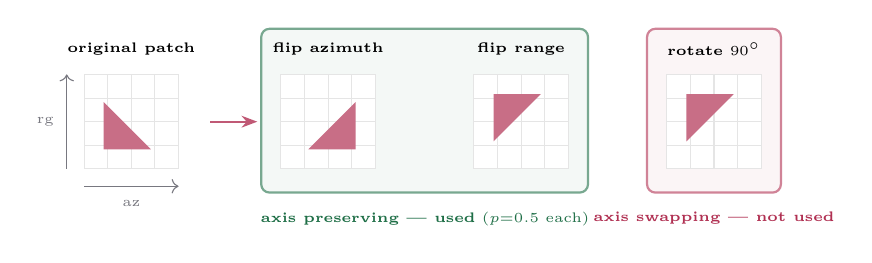
\begin{tikzpicture}
    \begin{scope}
      \node[font=\tiny\bfseries,anchor=south] at (0.6,1.32) {original patch};
      \draw[soft,thin,fill=white] (0,0) rectangle (1.2,1.2);
      \draw[black!10,step=0.3] (0,0) grid (1.2,1.2);
      \fill[accent!70] (0.25,0.25) -- (0.85,0.25) -- (0.25,0.85) -- cycle;
      \draw[->,soft] (-0.22,0) -- (-0.22,1.2);
      \node[font=\tiny,soft,anchor=east] at (-0.26,0.6) {rg};
      \draw[->,soft] (0,-0.22) -- (1.2,-0.22);
      \node[font=\tiny,soft,anchor=north] at (0.6,-0.28) {az};
    \end{scope}
    \draw[flow] (1.6,0.6) -- (2.2,0.6);
    \draw[good!60,thick,rounded corners=3pt,fill=good!5] (2.25,-0.3) rectangle (6.4,1.78);
    \node[font=\tiny,good,anchor=north] at (4.33,-0.42)
      {\textbf{axis preserving --- used} ($p{=}0.5$ each)};
    \begin{scope}[xshift=2.5cm]
      \node[font=\tiny\bfseries,anchor=south] at (0.6,1.32) {flip azimuth};
      \draw[soft,thin,fill=white] (0,0) rectangle (1.2,1.2);
      \draw[black!10,step=0.3] (0,0) grid (1.2,1.2);
      \fill[accent!70] (0.95,0.25) -- (0.35,0.25) -- (0.95,0.85) -- cycle;
    \end{scope}
    \begin{scope}[xshift=4.95cm]
      \node[font=\tiny\bfseries,anchor=south] at (0.6,1.32) {flip range};
      \draw[soft,thin,fill=white] (0,0) rectangle (1.2,1.2);
      \draw[black!10,step=0.3] (0,0) grid (1.2,1.2);
      \fill[accent!70] (0.25,0.95) -- (0.85,0.95) -- (0.25,0.35) -- cycle;
    \end{scope}
    \draw[accent!60,thick,rounded corners=3pt,fill=accent!5] (7.15,-0.3) rectangle (8.85,1.78);
    \node[font=\tiny,accent,anchor=north] at (8.0,-0.42)
      {\textbf{axis swapping --- not used}};
    \begin{scope}[xshift=7.4cm]
      \node[font=\tiny\bfseries,anchor=south] at (0.6,1.32) {rotate $90^\circ$};
      \draw[soft,thin,fill=white] (0,0) rectangle (1.2,1.2);
      \draw[black!10,step=0.3] (0,0) grid (1.2,1.2);
      \fill[accent!70] (0.25,0.95) -- (0.25,0.35) -- (0.85,0.95) -- cycle;
    \end{scope}
  \end{tikzpicture}
  \end{center}
  \begin{columns}[c]
    \begin{column}{0.52\textwidth}
      \begin{itemize}
        \item Flips are applied \textbf{jointly to input and target} ($p{=}0.5$ each):
              four orientations of every patch, spatial correspondence intact --- and
              each axis keeps its physical identity.
        \item Rotation would exchange range and azimuth --- two physically distinct
              axes (resolution, acquisition geometry, statistics) --- so only the
              axis-preserving pair is used.
      \end{itemize}
    \end{column}
    \begin{column}{0.46\textwidth}
      \centering
      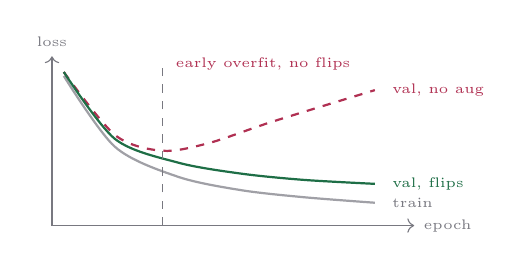
\begin{tikzpicture}
        \draw[->,soft] (0,0) -- (4.6,0) node[right,font=\tiny]{epoch};
        \draw[->,soft] (0,0) -- (0,2.15) node[above,font=\tiny]{loss};
        \draw[soft!70,thick] plot[smooth] coordinates
          {(0.15,1.9) (0.8,1.0) (1.6,0.62) (2.4,0.45) (3.2,0.36) (4.1,0.29)};
        \draw[accent,thick,dashed] plot[smooth] coordinates
          {(0.15,1.95) (0.8,1.15) (1.4,0.95) (2.0,1.05) (2.8,1.32) (4.1,1.72)};
        \draw[good,thick] plot[smooth] coordinates
          {(0.15,1.95) (0.8,1.1) (1.6,0.8) (2.4,0.66) (3.2,0.58) (4.1,0.53)};
        \draw[soft,dashed,thin] (1.4,0) -- (1.4,2.05);
        \node[font=\tiny,accent,anchor=south west] at (1.45,1.85) {early overfit, no flips};
        \node[font=\tiny,soft,anchor=west]   at (4.2,0.29) {train};
        \node[font=\tiny,good,anchor=west]   at (4.2,0.53) {val, flips};
        \node[font=\tiny,accent,anchor=west] at (4.2,1.72) {val, no aug};
      \end{tikzpicture}
      \\[1pt]
      {\scriptsize The flips push the validation turn-off point out --- the single-scene
       overfit arrives much later.}
    \end{column}
  \end{columns}
\end{frame}

% ---------------------------------------------------------------- 20b Augmentation verdict
\begin{frame}{Augmentation, measured --- flips delay the overfit and halve the seed spread}
    \centering
  {\scriptsize
  \renewcommand{\arraystretch}{0.78}
  \setlength{\tabcolsep}{6pt}
  \renewcommand{\seedtag}{augA}
  \begin{tabular}{@{}lccr@{}}
    \toprule
    metric & no aug & flips & $\Delta$ \\
    \midrule
    \multicolumn{4}{@{}l}{\emph{training (single scene, validation)}} \\
    best epoch (val) & 26.2    & \hlval{good}{\textbf{43.8}}    & \hlval{good}{$+17.6$}    \\
    best val loss $\downarrow$  & \seedpm{0.1443}{.0008} & \seedpm{\hlval{good}{0.1420}}{.0007} & \hlval{good}{$-0.0023$} \\
    \addlinespace[1pt]
    \multicolumn{4}{@{}l}{\emph{reconstruction (curve)}} \\
    curve $R^2$ $\uparrow$     & \seedpm{0.573}{.022} & \seedpm{0.569}{.008} & \textcolor{soft}{$-0.004$} \\
    curve MAE $\downarrow$     & \seedpm{0.0501}{.0012} & \seedpm{0.0496}{.0008} & \textcolor{soft}{$-0.0005$} \\
    PSNR [dB] $\uparrow$       & \seedpm{50.36}{.22} & \seedpm{50.32}{.08} & \textcolor{soft}{$-0.04$}  \\
    per-pixel $R^2$ $\uparrow$ & \seedpm{0.359}{.050} & \seedpm{0.359}{.031} & \textcolor{soft}{$-0.001$} \\
    profile cos med $\uparrow$ & \seedpm{0.851}{.020} & \seedpm{0.850}{.024} & \textcolor{soft}{$-0.001$} \\
    SSIM elev $\uparrow$       & \seedpm{0.9582}{.0009} & \seedpm{0.9586}{.0006} & \textcolor{soft}{$+0.0004$} \\
    SSIM range $\uparrow$      & \seedpm{0.9257}{.0027} & \seedpm{0.9258}{.0021} & \textcolor{soft}{$+0.0002$} \\
    SSIM azim $\uparrow$       & \seedpm{0.9457}{.0014} & \seedpm{0.9461}{.0012} & \textcolor{soft}{$+0.0004$} \\
    peak err mean $\downarrow$ & \seedpm{\textbf{4.47}}{.86} & \seedpm{4.70}{.47} & \textcolor{soft}{$+0.23$}  \\
    \quad median $\downarrow$  & \seedpm{0.94}{.37} & \seedpm{\textbf{0.81}}{.30} & \textcolor{soft}{$-0.13$}  \\
    \quad p95 $\downarrow$     & \seedpm{15.44}{.67} & \seedpm{15.44}{.47} & \textcolor{soft}{$+0.00$}  \\
    \addlinespace[1pt]
    \multicolumn{4}{@{}l}{\emph{detection (matched)}} \\
    precision $\uparrow$       & \seedpm{0.816}{.015} & \seedpm{0.821}{.008} & \textcolor{soft}{$+0.005$}  \\
    recall $\uparrow$          & \seedpm{0.656}{.056} & \seedpm{0.641}{.029} & \textcolor{soft}{$-0.015$} \\
    matched F1 $\uparrow$      & \seedpm{0.727}{.040} & \seedpm{0.720}{.020} & \textcolor{soft}{$-0.007$} \\
    count exact $\uparrow$     & \seedpm{0.611}{.066} & \seedpm{0.595}{.034} & \textcolor{soft}{$-0.016$} \\
    \addlinespace[1pt]
    \multicolumn{4}{@{}l}{\emph{seed-to-seed spread (std over 5 seeds)} $\downarrow$} \\
    recall            & .056 & \hlval{good}{\textbf{.029}} & \hlval{good}{$-48\%$} \\
    count exact       & .066 & \hlval{good}{\textbf{.034}} & \hlval{good}{$-49\%$} \\
    peak err mean     & .86  & \hlval{good}{\textbf{.47}}  & \hlval{good}{$-46\%$} \\
    per-pixel $R^2$   & .050 & \hlval{good}{\textbf{.031}} & \hlval{good}{$-38\%$} \\
    \bottomrule
  \end{tabular}}
  \par\vspace{1pt}
  \parbox{0.82\textwidth}{\tiny\color{soft} \textbf{runs}: UNet $\cdot$ conv $\cdot$ sorted-GT $\cdot$ $K{=}2$ $\cdot$ param-MSE $\cdot$ presence none $\cdot$ full norm ladder $\cdot$ patch $64{\times}32$ (aug = column); cells: mean $\pm$ std over five seeds. Training rows: validation split; others: held-out test, $5.0$\,M px. \textbf{bold} = better mean, marked only where the two differ by more than $5\%$; $\Delta =$ flips $-$ no aug, coloured (\textcolor{good}{gain} / \textcolor{accent}{cost}) only where $|\Delta|$ clears it; spread rows compare the seed stds; \textcolor{good}{green values} $=$ the training shift and the spread halving --- the effects that clear it. Peak median/p95: per-pixel peak-error distribution; cos med: median profile cosine; peak in elevation units.\par}

\end{frame}

% ---------------------------------------------------------------- 20b2 Augmentation by scatterer count
\begin{frame}{Augmentation by scatterer count --- no accuracy shift, half the spread}
    \centering
  \scriptsize
  \renewcommand{\arraystretch}{1.08}
  \setlength{\tabcolsep}{6pt}
  \renewcommand{\seedtag}{augB}
  \begin{tabular}{@{}l c c r@{}}
    \toprule
    metric & no aug & flips & $\Delta$ \\
    \midrule
    matched precision $\uparrow$ & \seedpm{0.816}{.015} & \seedpm{0.821}{.008} & \textcolor{soft}{$+0.005$} \\
    \quad $k{=}1$                & \seedpm{0.848}{.019} & \seedpm{0.853}{.008} & \textcolor{soft}{$+0.005$} \\
    \quad $k{=}2$                & \seedpm{0.776}{.013} & \seedpm{0.782}{.007} & \textcolor{soft}{$+0.006$} \\
    \addlinespace
    matched recall $\uparrow$    & \seedpm{0.656}{.056} & \seedpm{0.641}{\hlval{good}{.029}} & \textcolor{soft}{$-0.015$} \\
    \quad $k{=}1$                & \seedpm{0.647}{.088} & \seedpm{0.620}{\hlval{good}{.046}} & \textcolor{soft}{$-0.028$} \\
    \quad $k{=}2$                & \seedpm{0.670}{.016} & \seedpm{0.672}{\hlval{good}{.008}} & \textcolor{soft}{$+0.002$} \\
    \addlinespace
    count acc $\mid$ pred $k{=}1$ $\uparrow$ & \seedpm{0.952}{.009} & \seedpm{0.948}{.007} & \textcolor{soft}{$-0.004$} \\
    count acc $\mid$ pred $k{=}2$ $\uparrow$ & \seedpm{0.720}{.013} & \seedpm{0.733}{.010} & \textcolor{soft}{$+0.013$} \\
    \addlinespace
    matched $\mu$ MAE $\downarrow$ & \seedpm{2.30}{.12} & \seedpm{2.30}{.08} & \textcolor{soft}{$+0.00$} \\
    \quad $k{=}1$                & \seedpm{0.63}{.06} & \seedpm{\textbf{0.59}}{.04} & \textcolor{soft}{$-0.04$} \\
    \quad $k{=}2$                & \seedpm{4.07}{.05} & \seedpm{4.05}{.08} & \textcolor{soft}{$-0.02$} \\
    \addlinespace
    matched $\sigma$ MAE $\downarrow$ & \seedpm{0.86}{.05} & \seedpm{0.87}{.03} & \textcolor{soft}{$+0.01$} \\
    \quad $k{=}1$                & \seedpm{0.25}{.02} & \seedpm{0.25}{.01} & \textcolor{soft}{$+0.00$} \\
    \quad $k{=}2$                & \seedpm{1.51}{.01} & \seedpm{1.51}{.01} & \textcolor{soft}{$+0.00$} \\
    \addlinespace
    matched $a$ MAE $\downarrow$ & \seedpm{0.364}{.034} & \seedpm{0.374}{.026} & \textcolor{soft}{$+0.010$} \\
    \quad $k{=}1$                & \seedpm{0.155}{.029} & \seedpm{0.161}{.017} & \textcolor{soft}{$+0.006$} \\
    \quad $k{=}2$                & \seedpm{0.586}{.035} & \seedpm{0.593}{.022} & \textcolor{soft}{$+0.007$} \\
    \bottomrule
  \end{tabular}
  \par\vspace{3pt}
  \parbox{0.82\textwidth}{\tiny\color{soft} \textbf{runs}: UNet $\cdot$ conv $\cdot$ sorted-GT $\cdot$ $K{=}2$ $\cdot$ param-MSE $\cdot$ presence none $\cdot$ full norm ladder $\cdot$ patch $64{\times}32$ (aug = column); held-out test band, cells mean $\pm$ seed std over five seeded replicas; $k$ $=$ true scatterer count of the pixel. \textbf{bold} $=$ better mean, marked only where the two differ by more than $5\%$; $\Delta$ $=$ flips $-$ no aug, coloured only where $|\Delta|$ clears it; \textcolor{good}{green} $\pm$ $=$ the spread halving --- the one effect that does. Precision rewards under-prediction --- rank on recall. count acc $\mid$ pred $k$: share of pixels claiming exactly $k$ scatterers whose true count is $k$. $\mu$, $\sigma$ in elevation units; $a$ in linear amplitude.\par}
    

\end{frame}

% ---------------------------------------------------------------- 20b3 Augmentation: predicted stats vs GT
\begin{frame}{Augmentation, predicted statistics vs the GT --- same calibration, pinned down}
    \centering
  \scriptsize
  \renewcommand{\arraystretch}{1.00}
  \setlength{\tabcolsep}{6pt}
  \renewcommand{\seedtag}{augC}
  \begin{tabular}{@{}l !{\color{white}\vrule width 2pt} c !{\color{white}\vrule width 2pt} c c r@{}}
    \toprule
    prediction mean & \textcolor{good}{GT} & no aug & flips & $\Delta$ \\
    \midrule
    \multicolumn{5}{@{}l}{\textcolor{soft}{\emph{slot 0 --- strongest scatterer; GT-active on every pixel}}} \\
    \quad active frac            & 1.00    & \seedpm{0.706}{.066} & \seedpm{0.685}{\hlval{good}{.035}} & \textcolor{soft}{$-0.021$} \\
    \quad $a$ --- active         & 0.77    & \seedpm{0.89}{.07}   & \seedpm{0.90}{.03}   & \textcolor{soft}{$+0.01$} \\
    \quad $\mu$ --- active       & $-4.89$ & \seedpm{$-4.03$}{.15} & \seedpm{$-3.92$}{\hlval{good}{.10}} & \textcolor{soft}{$+0.11$} \\
    \quad $\sigma$ --- active    & 1.76    & \seedpm{1.52}{.08}   & \seedpm{1.48}{.05}   & \textcolor{soft}{$-0.04$} \\
    \addlinespace
    \multicolumn{5}{@{}l}{\textcolor{soft}{\emph{slot 1 --- second scatterer; GT-active on 26\% of pixels}}} \\
    \quad active frac            & 0.260 & \seedpm{0.306}{.008} & \seedpm{0.299}{.006} & \textcolor{soft}{$-0.007$} \\
    \quad $a$ --- active         & 1.43  & \seedpm{1.06}{.05} & \seedpm{1.04}{.03} & \textcolor{soft}{$-0.02$} \\
    \quad $a$ --- inact.         & 0.00  & \seedpm{0.45}{.04} & \seedpm{\textbf{0.42}}{\hlval{good}{.01}} & \textcolor{soft}{$-0.03$} \\
    \quad $\mu$ --- active       & 11.34 & \seedpm{9.97}{.40} & \seedpm{10.09}{.33} & \textcolor{soft}{$+0.12$} \\
    \quad $\mu$ --- inact.       & ---   & \seedpm{3.39}{.57} & \seedpm{4.09}{.31} & \textcolor{soft}{$+0.70$} \\
    \quad $\sigma$ --- active    & 3.53  & \seedpm{3.02}{.04} & \seedpm{2.94}{.05} & \textcolor{soft}{$-0.08$} \\
    \quad $\sigma$ --- inact.    & ---   & \seedpm{1.90}{.04} & \seedpm{1.87}{.03} & \textcolor{soft}{$-0.03$} \\
    \addlinespace
    \multicolumn{5}{@{}l}{\textcolor{soft}{\emph{distribution width --- std over GT-active pixels}}} \\
    \quad $a$ --- slot 0         & 1.48  & \seedpm{1.17}{.06} & \seedpm{1.17}{.03} & \textcolor{soft}{$+0.01$} \\
    \quad $\mu$ --- slot 0       & 3.30  & \seedpm{2.03}{.12} & \seedpm{1.99}{.07} & \textcolor{soft}{$-0.04$} \\
    \quad $\sigma$ --- slot 0    & 2.84  & \seedpm{\textbf{1.01}}{.03} & \seedpm{\hlval{accent}{0.95}}{.03} & \hlval{accent}{$-0.06$} \\
    \quad $a$ --- slot 1         & 1.45  & \seedpm{0.84}{.05} & \seedpm{0.83}{.04} & \textcolor{soft}{$-0.01$} \\
    \quad $\mu$ --- slot 1       & 16.24 & \seedpm{8.76}{.27} & \seedpm{8.72}{.18} & \textcolor{soft}{$-0.04$} \\
    \quad $\sigma$ --- slot 1    & 4.01  & \seedpm{\textbf{1.14}}{.04} & \seedpm{\hlval{accent}{1.07}}{.02} & \hlval{accent}{$-0.07$} \\
    \bottomrule
  \end{tabular}
  \par\vspace{3pt}
  \parbox{0.82\textwidth}{\tiny\color{soft} \textbf{runs}: UNet $\cdot$ conv $\cdot$ sorted-GT $\cdot$ $K{=}2$ $\cdot$ param-MSE $\cdot$ presence none $\cdot$ full norm ladder $\cdot$ patch $64{\times}32$ (aug = column); held-out test band, cells mean $\pm$ seed std over five seeded replicas; means conditioned on the slot's GT activity mask. \textbf{bold} $=$ closest to the \textcolor{good}{GT} column, marked only where best and worst differ by more than $5\%$; $\Delta$ $=$ flips $-$ no aug, coloured only where $|\Delta|$ clears it (\textcolor{accent}{cost} $=$ away from the GT); \textcolor{good}{green} $\pm$ $=$ the seed spreads flips pin down. Inactive GT slots define no $\mu$/$\sigma$ reference (---). Width rows: std of the prediction over GT-active pixels vs the GT's own std. $\mu$, $\sigma$ in elevation units; $a$ in linear amplitude.\par}
    

\end{frame}

% ---------------------------------------------------------------- 20c Augmentation loss curves
\begin{frame}{Augmentation --- the two loss curves}
  \begin{columns}[T]
    \begin{column}{0.5\textwidth}
      \centering
      {\small\textbf{\textcolor{accent}{no augmentation}}}\\[3pt]
      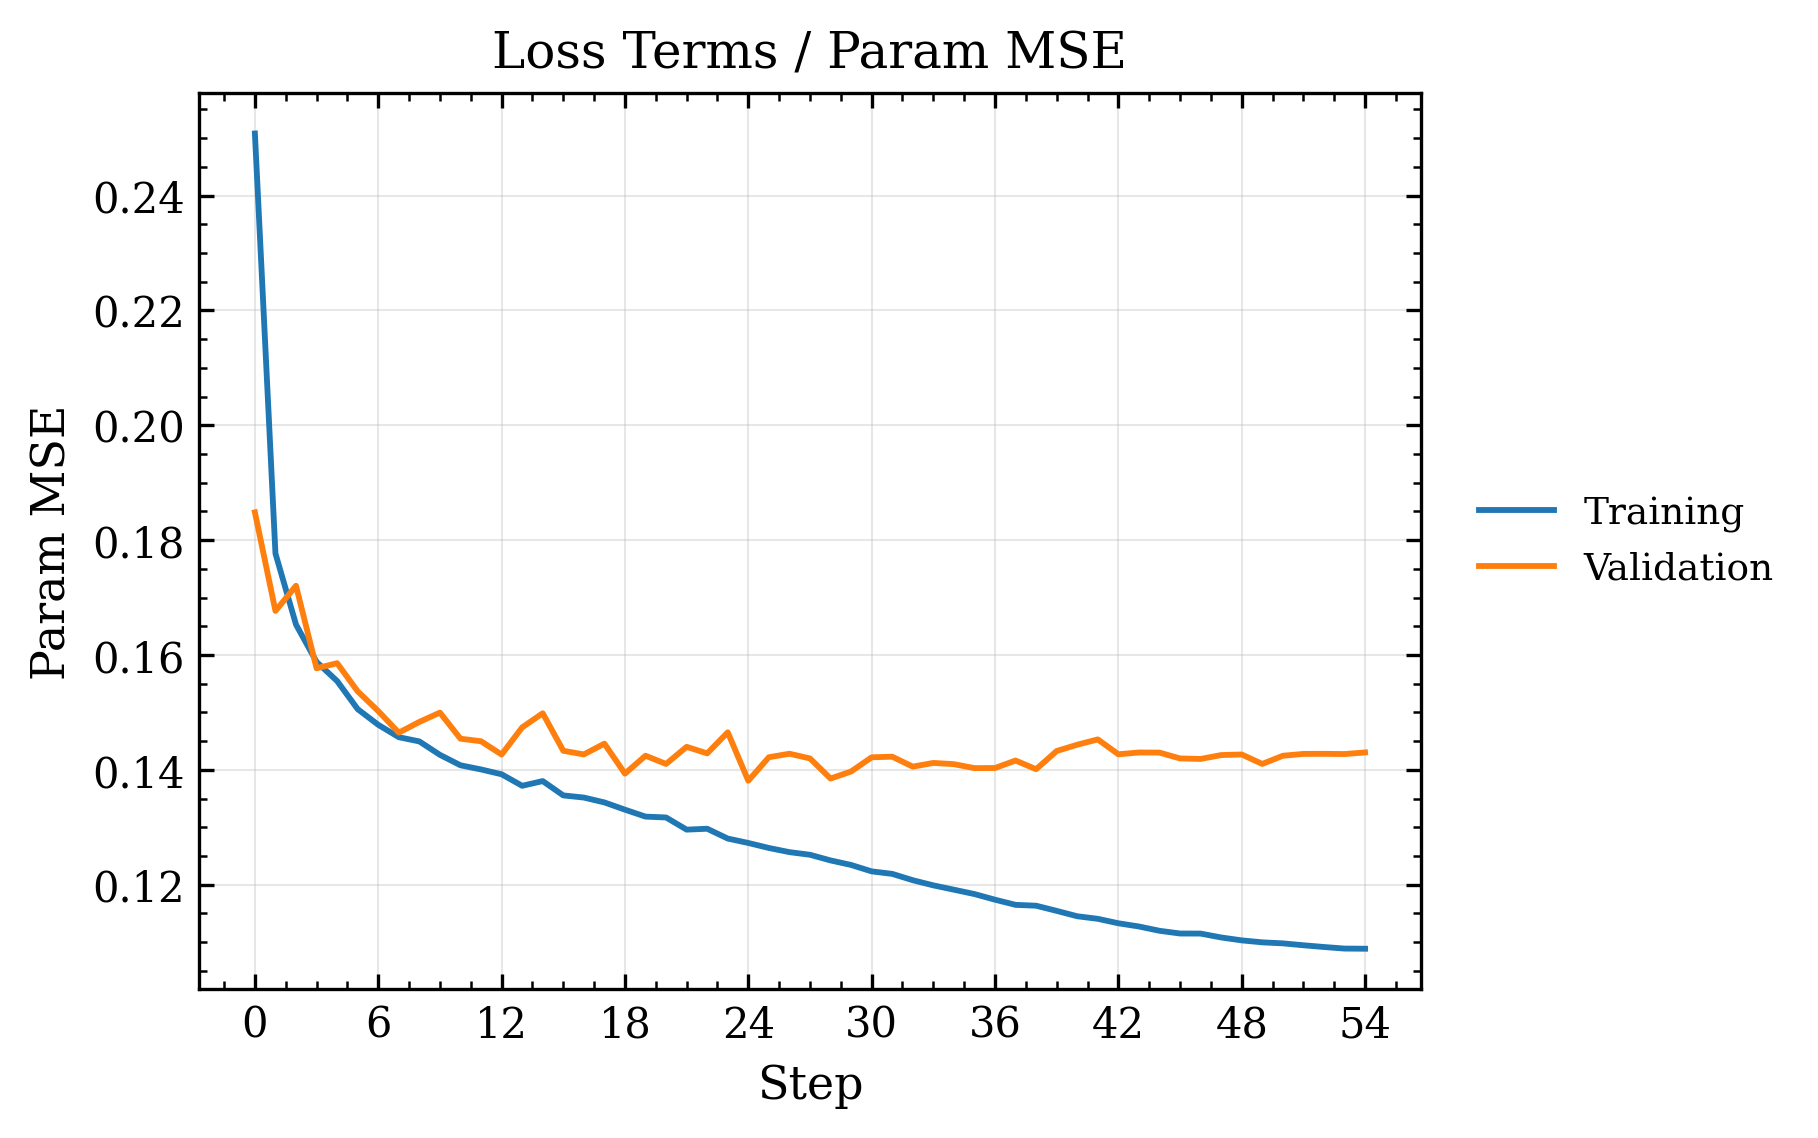
\includegraphics[width=\linewidth]{../figures/K2/augmentation_experiment/param_mse_no_aug.png}\\[3pt]
      {\scriptsize\color{soft} validation flattens early --- training pulls away, the single-scene overfit sets in.}
    \end{column}
    \begin{column}{0.5\textwidth}
      \centering
      {\small\textbf{\textcolor{good}{flips ($p{=}0.5$ each)}}}\\[3pt]
      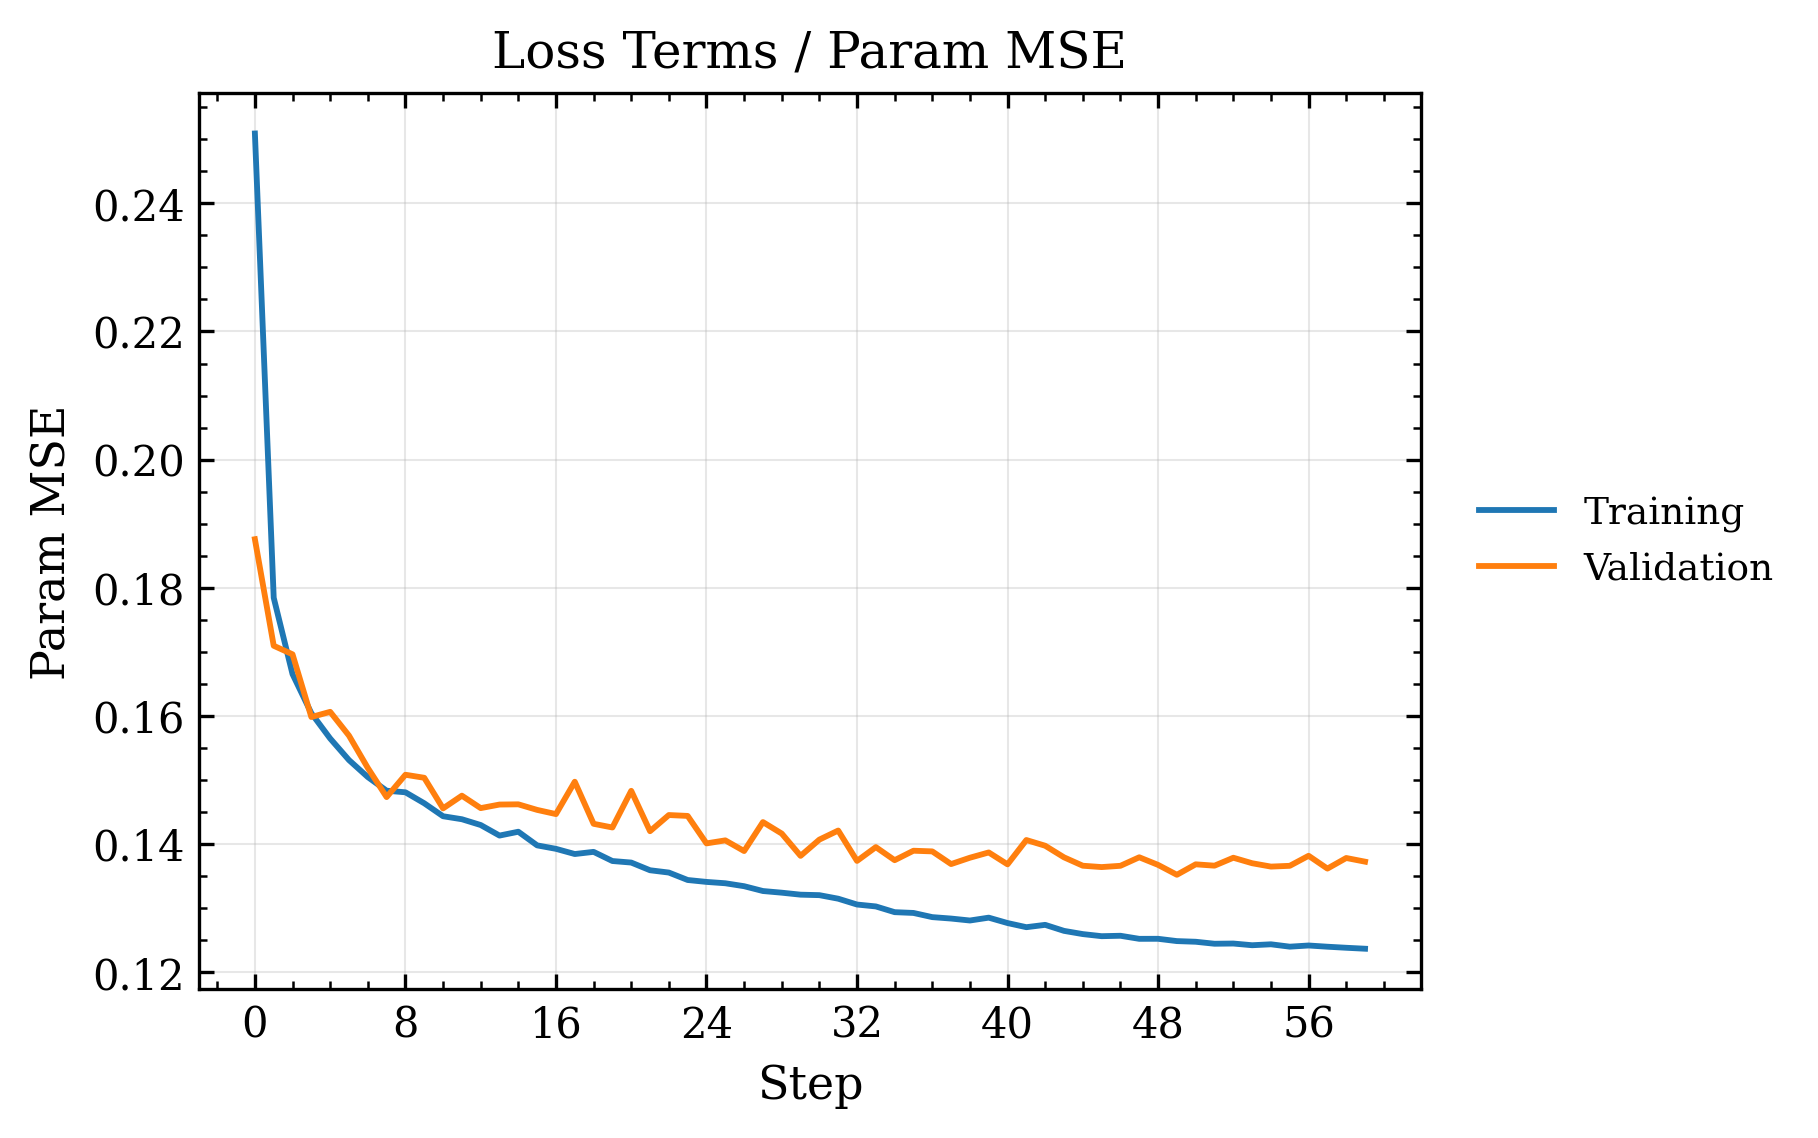
\includegraphics[width=\linewidth]{../figures/K2/augmentation_experiment/param_mse_aug.png}\\[3pt]
      {\scriptsize\color{soft} validation keeps descending --- the train--val gap stays narrow for longer.}
    \end{column}
  \end{columns}
\end{frame}


\act{IV \ \ What does the network actually need?}{context ladder \; $\cdot$ \; patch sizes \; $\cdot$ \; amplitude-only}

% ---------------------------------------------------------------- 22 Ladder design
\begin{frame}{The context ladder}
  \small
  TomoSAR theory inverts the \emph{expected} covariance per pixel; no estimator is
  per-pixel in the data. Every practical route --- the GT's own Capon included --- buys
  that expectation with a spatial window over the stack vectors $\mathbf{g} \in \mathbb{C}^{N}$:
  \begin{center}
  \vspace{-2pt}
  \begin{tabular}{ccc}
    {\scriptsize\color{soft} theory: one pixel, in expectation} & &
    {\scriptsize\color{soft} practice: $w_{a}{\times}w_{r}$ boxcar $B(x)$ (az${\times}$rg)} \\[3pt]
    $\mathbf{R}(x) \;=\; \mathrm{E}\big[\mathbf{g}(x)\,\mathbf{g}^{\mathsf H}(x)\big]$ &
    \quad$\longrightarrow$\quad &
    $\hat{\mathbf{R}}(x) \;=\; \dfrac{1}{w_{a}w_{r}} \displaystyle\sum_{x' \in B(x)} \mathbf{g}(x')\,\mathbf{g}^{\mathsf H}(x')$ \\
  \end{tabular}
  \vspace{-2pt}
  \end{center}
  \begin{center}
  \vspace{12pt}
  \begin{columns}[c,totalwidth=0.98\textwidth]
    \begin{column}{0.06\textwidth}
    \end{column}
    \begin{column}{0.60\textwidth}
      \centering
      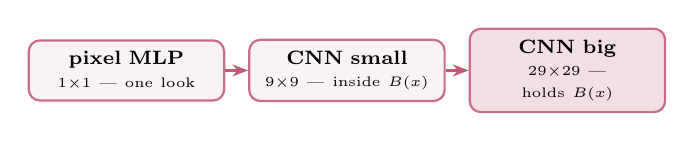
\begin{tikzpicture}
        \node[box, text width=22mm] (mlp) at (0,0)   {\textbf{pixel MLP}\\{\tiny $1{\times}1$ --- one look}};
        \node[box, text width=22mm] (c09) at (2.8,0) {\textbf{CNN small}\\{\tiny $9{\times}9$ --- inside $B(x)$}};
        \node[box, fill=accent!16, text width=22mm] (c29) at (5.6,0) {\textbf{CNN big}\\{\tiny $29{\times}29$ --- holds $B(x)$}};
        \draw[flow] (mlp) -- (c09);
        \draw[flow] (c09) -- (c29);
      \end{tikzpicture}
    \end{column}
    \begin{column}{0.32\textwidth}
      \centering
      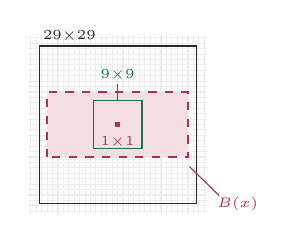
\begin{tikzpicture}[scale=0.86]
        \draw[black!7, step=0.08] (-1.32,-1.32) grid (1.32,1.32);
        \draw[ink, thin] (-1.16,-1.16) rectangle (1.16,1.16);
        \node[font=\tiny, text=ink, anchor=south west, inner sep=1pt] at (-1.15,1.17) {$29{\times}29$};
        \fill[accent!16] (-1.04,-0.48) rectangle (1.04,0.48);
        \draw[accent, semithick, dashed] (-1.04,-0.48) rectangle (1.04,0.48);
        \draw[good, thin] (-0.36,-0.36) rectangle (0.36,0.36);
        \draw[good, thin] (0,0.36) -- (0,0.60);
        \node[font=\tiny, text=good, anchor=south, inner sep=1pt] at (0,0.60) {$9{\times}9$};
        \fill[accent] (-0.04,-0.04) rectangle (0.04,0.04);
        \node[font=\tiny, text=accent, anchor=north, inner sep=3pt] at (0,-0.05) {$1{\times}1$};
        \draw[accent, thin] (1.06,-0.62) -- (1.50,-1.05);
        \node[font=\tiny, text=accent, anchor=north west, inner sep=1pt] at (1.42,-1.02) {$B(x)$};
      \end{tikzpicture}
    \end{column}
  \end{columns}
  \vspace{-15pt}
  \begin{columns}[t,totalwidth=0.98\textwidth]
    \begin{column}{0.06\textwidth}
    \end{column}
    \begin{column}{0.60\textwidth}
      \raggedright
      {\scriptsize to scale: $9{\times}9$ sits \emph{inside} the label's window;
       $29{\times}29$ is the first field to swallow it. One trunk, no downsampling,
       \textbf{capacity held at ${\sim}31$\,M} on every rung --- the receptive field
       is the only thing that moves.\par}
    \end{column}
    \begin{column}{0.32\textwidth}
    \end{column}
  \end{columns}
  \end{center}
\end{frame}

% ---------------------------------------------------------------- 22b Why the ladder must help
\begin{frame}{Why the ladder must help --- the label is a window statistic}
  \setlength{\abovedisplayskip}{4pt}
  \setlength{\belowdisplayskip}{4pt}
  \small
  \setlength{\arrayrulewidth}{0.3pt}
  \arrayrulecolor{soft!60}
  \vspace{12pt}
  \begin{tabular}{@{}p{0.437\textwidth}@{\hspace{15pt}}|@{\hspace{17pt}}p{0.437\textwidth}@{}}
    \textbf{1. The label is $B(x)$-measurable.} Capon and the parameter fit are
    deterministic maps, so
    \[
      y(x) \;=\; \Phi\big(\mathbf{g}_{B(x)}\big),
    \]
    exactly, by construction --- no assumption on the scene. The label holds no
    randomness the looks in $B(x)$ do not already hold.
    \rule[-16pt]{0pt}{0pt}%
    &
    \textbf{2. The error splits into a floor and a fit.} For \emph{any} predictor
    $\hat y$ built from a field $\mathcal{F}$,
    \[
      \begin{aligned}
        \mathrm{E}\big[(y - \hat y)^{2}\big] = {}
          & \mathrm{E}\big[\mathrm{Var}(y \mid \mathbf{g}_{\mathcal{F}})\big] \\[2pt]
          & + \mathrm{E}\big[(\mathrm{E}[y \mid \mathbf{g}_{\mathcal{F}}] - \hat y)^{2}\big].
      \end{aligned}
    \]
    The first term is the \textbf{floor}, fixed by $\mathcal{F}$ alone; the second is
    what training buys.
    \rule[-16pt]{0pt}{0pt}%
    \\
    \hline
    \rule{0pt}{24pt}%
    \textbf{3. The floor only falls.} Take any two rungs with $\mathcal{F}_{1}
    \subseteq \mathcal{F}_{2}$ and condition once more on the wider one:
    \[
      \begin{aligned}
        \mathrm{Var}(y \mid \mathbf{g}_{\mathcal{F}_1}) = {}
          & \mathrm{E}\big[\mathrm{Var}(y \mid \mathbf{g}_{\mathcal{F}_2}) \mid \mathbf{g}_{\mathcal{F}_1}\big] \\[2pt]
          & + \mathrm{Var}\big(\mathrm{E}[y \mid \mathbf{g}_{\mathcal{F}_2}] \mid \mathbf{g}_{\mathcal{F}_1}\big).
      \end{aligned}
    \]
    The last term is a variance, hence $\ge 0$:
    \[
      \mathrm{E}\big[\mathrm{Var}(y \mid \mathbf{g}_{\mathcal{F}_1})\big]
      \;\ge\;
      \mathrm{E}\big[\mathrm{Var}(y \mid \mathbf{g}_{\mathcal{F}_2})\big].
    \]
    &
    \rule{0pt}{24pt}%
    \textbf{4. And it vanishes.} Once the field holds the whole window, the label's
    own looks are among those handed to the model:
    \[
      \begin{aligned}
        B(x) \subseteq \mathcal{F}
          &\;\Longrightarrow\; \mathbf{g}_{B(x)} \subseteq \mathbf{g}_{\mathcal{F}} \\[1pt]
          &\;\Longrightarrow\; y = \Phi(\mathbf{g}_{B(x)}) \text{ fixed by } \mathbf{g}_{\mathcal{F}} \\[1pt]
          &\;\Longrightarrow\; \mathrm{Var}(y \mid \mathbf{g}_{\mathcal{F}}) = 0.
      \end{aligned}
    \]
    \\
  \end{tabular}
\end{frame}

% ---------------------------------------------------------------- 22c The bottom rung
\begin{frame}{The floor of any field --- the fluctuation of the looks it misses}
  \begin{columns}[c]
    \begin{column}{0.47\textwidth}
      \small
      \setlength{\abovedisplayskip}{11pt}
      \setlength{\belowdisplayskip}{22pt}
      Take \emph{any} field $\mathcal{F}$ and split the label's window into the
      looks the field delivers and the looks it misses:
      \[
        w_{a}w_{r}\,\hat{\mathbf{R}}(x) \;=\; \left\{
        \begin{aligned}
          & \sum_{p \in B(x) \cap \mathcal{F}} \mathbf{g}(p)\mathbf{g}^{\mathsf H}(p) \\[2pt]
          & + \sum_{p \in B(x) \setminus \mathcal{F}} \mathbf{g}(p)\mathbf{g}^{\mathsf H}(p).
        \end{aligned}
        \right.
      \]
      The first sum is delivered, the second is missed. Which pixels fall in which
      is the \emph{only} thing that changes along the ladder.
      Condition on $\mathbf{g}_{\mathcal{F}}$. Every look in the first sum is one
      the field hands over, so that term is a constant and carries no variance ---
      only the misses fluctuate:
    \end{column}
    \begin{column}{0.47\textwidth}
      \small
      \setlength{\abovedisplayskip}{11pt}
      \setlength{\belowdisplayskip}{22pt}
      \[
        \begin{aligned}
          &\mathrm{Var}\big(\hat{\mathbf{R}}(x) \,\big|\, \mathbf{g}_{\mathcal{F}}\big) \\[5pt]
          &\quad = \mathrm{Var}\bigg(\frac{1}{w_{a}w_{r}}\sum_{p \in B(x) \cap \mathcal{F}} \mathbf{g}(p)\mathbf{g}^{\mathsf H}(p) \\[2pt]
          &\qquad\qquad + \frac{1}{w_{a}w_{r}}\sum_{p \in B(x) \setminus \mathcal{F}} \mathbf{g}(p)\mathbf{g}^{\mathsf H}(p)
            \,\bigg|\, \mathbf{g}_{\mathcal{F}}\bigg) \\[5pt]
          &\quad = \boxed{\;\frac{1}{(w_{a}w_{r})^{2}}\,\mathrm{Var}\bigg(
            \sum_{p \in B(x) \setminus \mathcal{F}} \mathbf{g}(p)\mathbf{g}^{\mathsf H}(p)
            \,\bigg|\, \mathbf{g}_{\mathcal{F}}\bigg)\;}
        \end{aligned}
      \]
      Exact: no assumption on the scene, no independence between looks. And when
      $B(x) \setminus \mathcal{F} = \varnothing$ the sum is empty --- the floor is
      $0$.
    \end{column}
  \end{columns}
\end{frame}

% ---------------------------------------------------------------- 22d The three rungs
\begin{frame}{The three rungs --- only one term moves}
  \vfill
  \begin{center}
  {\small
  \renewcommand{\arraystretch}{1.8}
  \setlength{\tabcolsep}{10pt}
  \begin{tabular}{@{}l c c c@{}}
    \toprule
      & \textbf{pixel MLP} & \textbf{CNN small} & \textbf{CNN big} \\
      & $r = 1$
      & $r < w_{r}$
      & $r \ge w_{a}$ \\
    \midrule
    misses $\big|B(x) \setminus \mathcal{F}\big|$
      & $w_{a}w_{r} - 1$
      & $w_{a}w_{r} - r^{2}$
      & $0$ \\
    \rowcolor{argA!22}
    label variance $\mathrm{E}\big[\mathrm{Var}(y \mid \mathbf{g}_{\mathcal{F}})\big]$
      & the misses fluctuate
      & the misses fluctuate
      & $\mathbf{0}$ \\
    model error $\mathrm{E}\big[(\mathrm{E}[y \mid \mathbf{g}_{\mathcal{F}}] - \hat y)^{2}\big]$
      & training buys
      & training buys
      & training buys \\
    \midrule
    total $\mathrm{E}\big[(y - \hat y)^{2}\big]$
      & floor $+$ model
      & floor $+$ model
      & \textbf{model alone} \\
    \bottomrule
  \end{tabular}}
  \end{center}
  \vspace{6pt}
  {\footnotesize\raggedright Every column is the same quantity,
   $w_{a}w_{r} - \big|B(x) \cap \mathcal{F}\big|$ --- the control meets the window in
   a single pixel, the small CNN in all $r^{2}$ of its field, the big CNN in the whole
   of it. Only the shaded row moves, and no architecture or loss touches it; model
   error reads the same in every column, and capacity is held fixed across the ladder,
   so the field is the only variable.
   \par}
  \vfill
\end{frame}

% ---------------------------------------------------------------- 23 Ladder result
\begin{frame}{Ladder result: context grounds the prediction}
  \centering
  \scriptsize
  \renewcommand{\arraystretch}{1.02}
  \setlength{\tabcolsep}{6pt}
  \begin{tabular}{@{}l c r@{\hskip 6pt}l r@{\hskip 6pt}l@{}}
    \toprule
    metric & pixel MLP & \multicolumn{2}{c}{CNN small \; ($\Delta$)} & \multicolumn{2}{c@{}}{CNN big \; ($\Delta$)} \\
    {\color{soft} field $\mathcal{F}$ / looks seen}
      & {\color{soft} $1{\times}1$ / $1$}
      & \multicolumn{2}{c}{\color{soft} $9{\times}9$ / $81$}
      & \multicolumn{2}{c@{}}{\color{soft} $29{\times}29$ / $312$} \\
    \midrule
    curve $R^2$ $\uparrow$                   & 0.24    & 0.47           & \hlval{good}{$+0.23$}    & \textbf{0.59}  & \hlval{good}{$+0.12$}  \\
    per-pixel $R^2$ (median) $\uparrow$      & \hlval{accent}{$-0.03$} & 0.42           & \hlval{good}{$+0.45$}    & \textbf{0.57}  & \hlval{good}{$+0.15$}  \\
    \addlinespace
    SSIM elevation $\uparrow$                & 0.918   & 0.949          & \hlval{good}{$+0.031$}   & 0.958 & \hlval{good}{$+0.009$} \\
    SSIM range $\uparrow$                    & 0.869   & 0.917          & \hlval{good}{$+0.048$}   & \textbf{0.928} & \hlval{good}{$+0.011$} \\
    SSIM azimuth $\uparrow$                  & 0.895   & 0.934          & \hlval{good}{$+0.039$}   & \textbf{0.944} & \hlval{good}{$+0.010$} \\
    peak error median [units] $\downarrow$   & 2.01    & \textbf{0.67}  & \hlval{good}{$-1.34$}    & \textbf{0.67}  & \textcolor{soft}{$0.00$}   \\
    \addlinespace
    matched recall $\uparrow$                & 0.61    & \textbf{0.69}  & \hlval{good}{$+0.08$}    & 0.68           & \hlval{accent}{$-0.01$} \\
    \quad 2 scatterers $\uparrow$            & 0.55    & 0.63           & \hlval{good}{$+0.08$}    & \textbf{0.70}  & \hlval{good}{$+0.06$}  \\
    count exact $\uparrow$                   & 0.56    & \textbf{0.68}  & \hlval{good}{$+0.12$}    & 0.62           & \hlval{accent}{$-0.06$} \\
    \addlinespace
    matched $\mu$ MAE [units] $\downarrow$   & 3.37    & 2.37           & \hlval{good}{$-1.00$}    & \textbf{2.12}  & \hlval{good}{$-0.25$}  \\
    \quad 2 scatterers $\downarrow$          & 5.70    & 4.30           & \hlval{good}{$-1.41$}    & \textbf{3.79}  & \hlval{good}{$-0.51$}  \\
    matched $\sigma$ MAE $\downarrow$        & 1.21    & 0.86           & \hlval{good}{$-0.35$}    & \textbf{0.84}  & \hlval{good}{$-0.02$}  \\
    \quad 2 scatterers $\downarrow$          & 2.01    & 1.59           & \hlval{good}{$-0.42$}    & \textbf{1.49}  & \hlval{good}{$-0.10$}  \\
    matched $a$ MAE $\downarrow$             & 0.531   & \textbf{0.326} & \hlval{good}{$-0.205$}   & 0.334          & \hlval{accent}{$+0.008$} \\
    \bottomrule
  \end{tabular}
  \par\smallskip
  \parbox{0.82\textwidth}{\tiny\color{soft} \textbf{runs}: conv head $\cdot$ sorted-GT $\cdot$ $K{=}2$ $\cdot$ param-MSE $\cdot$ active-norm $\cdot$ no aug (model = column).
   Looks seen out of $|B(x)| = w_{a}w_{r} = 26 \times 12 = 312$.
   Held-out test, $5.0$\,M px; \textbf{bold} = best, marked only where best and worst differ by more than $5\%$;
   $\Delta$ vs previous tier (\textcolor{good}{better} / \textcolor{accent}{worse}); \textcolor{accent}{red value} $=$ the $1{\times}1$ control regressing its conditional mean\par}
    

\end{frame}

% ---------------------------------------------------------------- 24b Correlation law
\begin{frame}{The correlation law --- how labels share their inputs}
  \setlength{\abovedisplayskip}{3pt}
  \setlength{\belowdisplayskip}{3pt}
  \begin{columns}[c,onlytextwidth]
    \begin{column}{0.46\textwidth}
      \centering
      {\scriptsize\textbf{Azimuth}: slide the second window along track.\par}
      \vspace{1pt}
      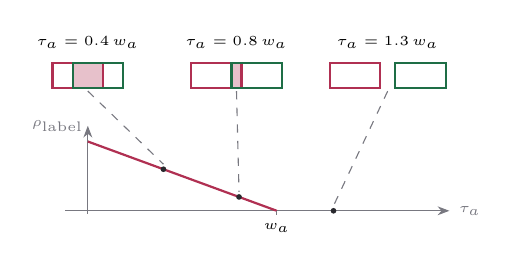
\begin{tikzpicture}[scale=0.80]
        \fill[accent!30] (0.42,1.95) rectangle (0.90,2.35);
        \draw[accent, thick] (0.10,1.95) rectangle ++(0.8,0.4);
        \draw[good, thick]   (0.42,1.95) rectangle ++(0.8,0.4);
        \node[font=\tiny, anchor=south] at (0.66,2.42) {$\tau_{a} = 0.4\,w_{a}$};
        \fill[accent!30] (2.94,1.95) rectangle (3.10,2.35);
        \draw[accent, thick] (2.30,1.95) rectangle ++(0.8,0.4);
        \draw[good, thick]   (2.94,1.95) rectangle ++(0.8,0.4);
        \node[font=\tiny, anchor=south] at (3.02,2.42) {$\tau_{a} = 0.8\,w_{a}$};
        \draw[accent, thick] (4.50,1.95) rectangle ++(0.8,0.4);
        \draw[good, thick]   (5.54,1.95) rectangle ++(0.8,0.4);
        \node[font=\tiny, anchor=south] at (5.42,2.42) {$\tau_{a} = 1.3\,w_{a}$};
        \draw[soft, dashed, thin] (0.66,1.90) -- (1.86,0.74);
        \draw[soft, dashed, thin] (3.02,1.90) -- (3.06,0.30);
        \draw[soft, dashed, thin] (5.42,1.90) -- (4.56,0.08);
        \draw[-{Stealth[length=1.5mm]}, soft] (0.30,0) -- (6.40,0)
          node[right,font=\tiny]{$\tau_{a}$};
        \draw[-{Stealth[length=1.5mm]}, soft] (0.66,-0.05) -- (0.66,1.35)
          node[anchor=east, font=\tiny, inner sep=1.5pt]{$\rho_{\text{label}}$};
        \draw[accent, thick] (0.66,1.10) -- (3.66,0);
        \draw[soft] (3.66,0) -- (3.66,-0.06);
        \node[font=\tiny, anchor=north] at (3.66,-0.05) {$w_{a}$};
        \fill[ink] (1.86,0.66) circle (0.045);
        \fill[ink] (3.06,0.22) circle (0.045);
        \fill[ink] (4.56,0.00) circle (0.045);
      \end{tikzpicture}\\[6pt]
      {\scriptsize\textbf{Range}: the same construction, across track.\par}
      \vspace{1pt}
      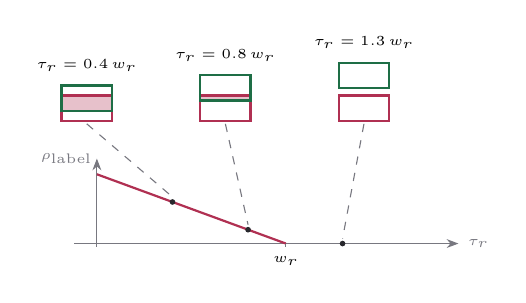
\begin{tikzpicture}[scale=0.80]
        \fill[accent!30] (0.10,2.11) rectangle (0.90,2.35);
        \draw[accent, thick] (0.10,1.95) rectangle ++(0.8,0.4);
        \draw[good, thick]   (0.10,2.11) rectangle ++(0.8,0.4);
        \node[font=\tiny, anchor=south] at (0.50,2.58) {$\tau_{r} = 0.4\,w_{r}$};
        \fill[accent!30] (2.30,2.27) rectangle (3.10,2.35);
        \draw[accent, thick] (2.30,1.95) rectangle ++(0.8,0.4);
        \draw[good, thick]   (2.30,2.27) rectangle ++(0.8,0.4);
        \node[font=\tiny, anchor=south] at (2.70,2.74) {$\tau_{r} = 0.8\,w_{r}$};
        \draw[accent, thick] (4.50,1.95) rectangle ++(0.8,0.4);
        \draw[good, thick]   (4.50,2.47) rectangle ++(0.8,0.4);
        \node[font=\tiny, anchor=south] at (4.90,2.94) {$\tau_{r} = 1.3\,w_{r}$};
        \draw[soft, dashed, thin] (0.50,1.90) -- (1.86,0.74);
        \draw[soft, dashed, thin] (2.70,1.90) -- (3.06,0.30);
        \draw[soft, dashed, thin] (4.90,1.90) -- (4.56,0.08);
        \draw[-{Stealth[length=1.5mm]}, soft] (0.30,0) -- (6.40,0)
          node[right,font=\tiny]{$\tau_{r}$};
        \draw[-{Stealth[length=1.5mm]}, soft] (0.66,-0.05) -- (0.66,1.35)
          node[anchor=east, font=\tiny, inner sep=1.5pt]{$\rho_{\text{label}}$};
        \draw[accent, thick] (0.66,1.10) -- (3.66,0);
        \draw[soft] (3.66,0) -- (3.66,-0.06);
        \node[font=\tiny, anchor=north] at (3.66,-0.05) {$w_{r}$};
        \fill[ink] (1.86,0.66) circle (0.045);
        \fill[ink] (3.06,0.22) circle (0.045);
        \fill[ink] (4.56,0.00) circle (0.045);
      \end{tikzpicture}
\end{column}
    \begin{column}{0.54\textwidth}
      \small
      {\scriptsize The shaded overlap \emph{is} the correlation --- each case drops
       onto the triangle. Same law on both axes, each dying at its own $w$.\par}
      \vspace{4pt}
      \begin{itemize}\setlength{\itemsep}{11pt}
        \item \textbf{The label}: a $w_{a}{\times}w_{r}$ boxcar covariance around
              its pixel (az${\times}$rg) --- every pixel of $B(x)$ enters the
              label at $x$, and nothing outside $B(x)$ does.
        \item \textbf{The correlation law}: two labels share input pixels
              in proportion to how far their boxcars overlap. The boxcar is a
              product of two intervals, so the law is separable:
              \[
                \rho_{\text{label}}(\tau_{a}, \tau_{r}) =
                \big(1 - \tau_{a}/w_{a}\big)_{+}\big(1 - \tau_{r}/w_{r}\big)_{+},
              \]
              vanishing once $\tau_{a} = w_{a}$ \emph{or} $\tau_{r} = w_{r}$: past
              either the windows are disjoint and the labels share nothing.
      \end{itemize}
    \end{column}
  \end{columns}
\end{frame}

% ---------------------------------------------------------------- 24b2 Reading the reach
\begin{frame}{Reading the reach --- the network estimates statistics}
  \begin{columns}[c]
    \begin{column}{0.05\textwidth}
    \end{column}
    \begin{column}{0.42\textwidth}
      \centering
      {\scriptsize two labels at offset $\Delta$ split into shared and
       private looks:\par}
      \vspace{4pt}
      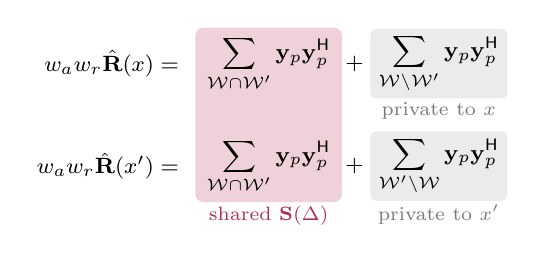
\begin{tikzpicture}[font=\footnotesize, baseline,
          box/.style={rounded corners=2pt, inner xsep=3pt, inner ysep=2pt},
          lbl/.style={font=\scriptsize, inner sep=1pt, anchor=north}]
        \node[anchor=east] (ex) at (0,0)    {$w_{a}w_{r}\hat{\mathbf R}(x) =$};
        \node[anchor=east] (ey) at (0,-1.3) {$w_{a}w_{r}\hat{\mathbf R}(x') =$};
        \node[box, anchor=west] (sx) at (0.12,0)    {$\displaystyle\sum_{\mathcal W\cap\mathcal W'}\mathbf y_p\mathbf y_p^{\mathsf H}$};
        \node[box, anchor=west] (sy) at (0.12,-1.3) {$\displaystyle\sum_{\mathcal W\cap\mathcal W'}\mathbf y_p\mathbf y_p^{\mathsf H}$};
        \node[anchor=west, inner xsep=2pt] (px) at (sx.east) {$+$};
        \node[anchor=west, inner xsep=2pt] (py) at (sy.east) {$+$};
        \node[box, fill=black!8, anchor=west] (dx) at (px.east) {$\displaystyle\sum_{\mathcal W\setminus\mathcal W'}\mathbf y_p\mathbf y_p^{\mathsf H}$};
        \node[box, fill=black!8, anchor=west] (dy) at (py.east) {$\displaystyle\sum_{\mathcal W'\setminus\mathcal W}\mathbf y_p\mathbf y_p^{\mathsf H}$};
        \begin{scope}[on background layer]
          \node[fit=(sx)(sy), fill=accent!22, rounded corners=3pt, inner sep=1pt] (sh) {};
        \end{scope}
        \node[lbl, text=accent, anchor=north] at (sh.south) {shared $\mathbf S(\Delta)$};
        \node[lbl, text=soft] at (dx.south) {private to $x$};
        \node[lbl, text=soft] at (dy.south) {private to $x'$};
      \end{tikzpicture}\\[12pt]
      {\scriptsize the shared fraction at every offset $\tau$ is the
       correlation law:\par}
      \vspace{2pt}
      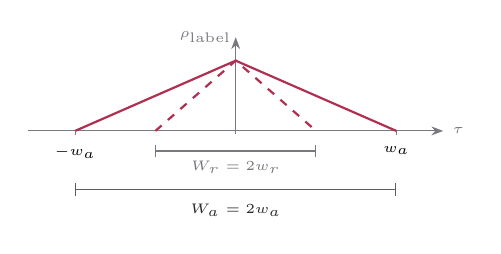
\begin{tikzpicture}[scale=0.85]
        \draw[-{Stealth[length=1.5mm]}, soft] (-3.1,0) -- (3.1,0) node[right,font=\tiny]{$\tau$};
        \draw[-{Stealth[length=1.5mm]}, soft] (0,-0.05) -- (0,1.40)
          node[anchor=east, font=\tiny, inner sep=1.5pt]{$\rho_{\text{label}}$};
        \draw[accent, thick]         (-2.4,0) -- (0,1.05) -- (2.4,0);
        \draw[accent, thick, dashed] (-1.2,0) -- (0,1.05) -- (1.2,0);
        \draw[soft, thin] (-2.4,0) -- (-2.4,-0.06);
        \draw[soft, thin] (2.4,0) -- (2.4,-0.06);
        \node[font=\tiny, anchor=north] at (-2.4,-0.08) {$-w_{a}$};
        \node[font=\tiny, anchor=north] at (2.4,-0.08) {$w_{a}$};
        \draw[|-|, ink!75] (-2.4,-0.88) -- (2.4,-0.88);
        \node[font=\tiny, text=ink, anchor=north] at (0,-0.95) {$W_{a} = 2w_{a}$};
        \draw[|-|, soft] (-1.2,-0.30) -- (1.2,-0.30);
        \node[font=\tiny, text=soft, anchor=north] at (0,-0.30) {$W_{r} = 2w_{r}$};
      \end{tikzpicture}\\[2pt]
      {\scriptsize the label correlates over $\pm w_{a}$ in azimuth and
       $\pm w_{r}$ in range --- the centred patch spanning both triangles is
       $W_{a}{\times}W_{r}$.\par}
    \end{column}
    \begin{column}{0.51\textwidth}
      \centering
      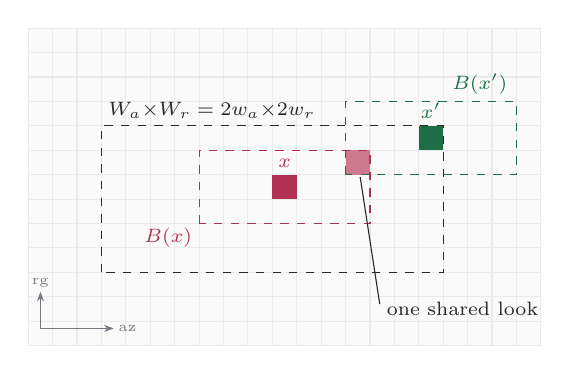
\begin{tikzpicture}[scale=1.55]
        \draw[soft, thin, fill=black!2] (0,0) rectangle (4.2,2.6);
        \draw[black!8, step=0.2] (0,0) grid (4.2,2.6);
        \fill[accent!65] (2.60,1.40) rectangle ++(0.2,0.2);
        \fill[accent] (2.00,1.20) rectangle ++(0.2,0.2);
        \fill[good] (3.20,1.60) rectangle ++(0.2,0.2);
        \draw[ink, dashed, thin] (0.60,0.60) rectangle ++(2.8,1.2);
        \node[font=\scriptsize, text=ink, anchor=south west, inner sep=1.5pt] at (0.62,1.82) {$W_{a}{\times}W_{r} = 2w_{a}{\times}2w_{r}$};
        \draw[accent, dashed, thin] (1.40,1.00) rectangle ++(1.4,0.6);
        \node[font=\scriptsize, text=accent, anchor=north east, inner sep=1.5pt] at (1.38,1.00) {$B(x)$};
        \node[font=\scriptsize, text=accent, anchor=south, inner sep=1.5pt] at (2.10,1.42) {$x$};
        \draw[good, dashed, thin] (2.60,1.40) rectangle ++(1.4,0.6);
        \node[font=\scriptsize, text=good, anchor=south, inner sep=1.5pt] at (3.70,2.02) {$B(x')$};
        \node[font=\scriptsize, text=good, anchor=south, inner sep=1.5pt] at (3.30,1.82) {$x'$};
        \node[font=\scriptsize, text=ink, anchor=west, inner sep=1.5pt] at (2.90,0.30) {one shared look};
        \draw[ink, thin] (2.88,0.34) -- (2.72,1.38);
        \draw[-{Stealth[length=1.2mm]}, soft] (0.10,0.14) -- (0.70,0.14)
          node[right, font=\tiny, inner sep=1.5pt] {az};
        \draw[-{Stealth[length=1.2mm]}, soft] (0.10,0.14) -- (0.10,0.44)
          node[above, font=\tiny, inner sep=1.5pt] {rg};
      \end{tikzpicture}\\[4pt]
      {\scriptsize $x'$ sits at the far corner of the patch: $B(x')$ keeps a
       single shared look with $B(x)$ --- one step further and the windows are
       disjoint ($|\Delta_{a}| = w_{a}$ \emph{or} $|\Delta_{r}| = w_{r}$).}
    \end{column}
  \end{columns}
\end{frame}

% ---------------------------------------------------------------- 24c Sweep verdict
\begin{frame}{The verdict --- saturation at the reach, axis by axis}
  \centering
  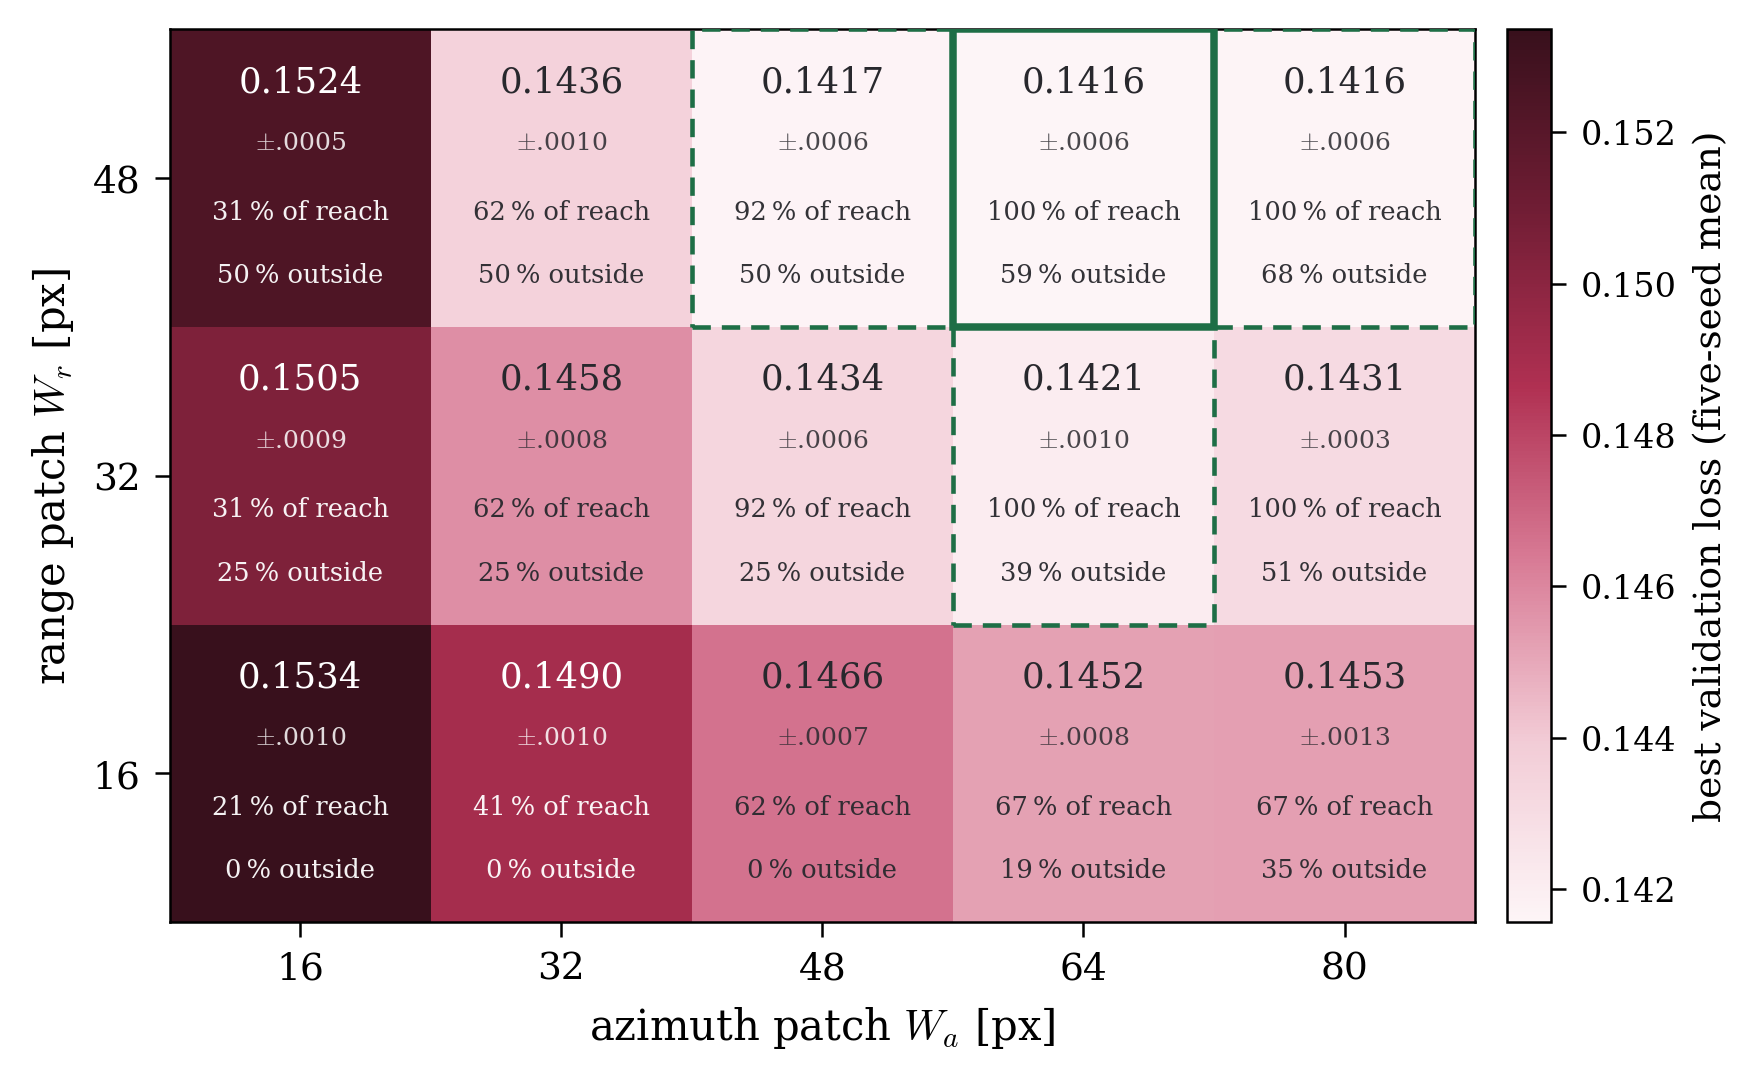
\includegraphics[width=0.56\linewidth]{../figures/K2/Patch/patch_sweep_loss_heatmap.png}
  \par\vspace{4pt}
  {\scriptsize
  \setlength{\tabcolsep}{6pt}
  \begin{tabular}{@{}lll@{}}
    \toprule
                 & registered  & observed \\
    \midrule
    azimuth knee & $2w_a = 52$ & $\mathbf{48}$--$\mathbf{64}$, flat past $48$ \\
    \addlinespace[2pt]
    range knee   & $2w_r = 24$ & $\mathbf{32}$; $\le 0.002$ left to $48$ \\
    \bottomrule
  \end{tabular}}
  \par\vspace{4pt}
  \parbox{0.82\textwidth}{\scriptsize\color{soft} \textbf{runs}: patch $W_a{\times}W_r$ $=$ cell, all else fixed (full input stack, $26{\times}12$ boxcar labels); five seeded replicas per cell, cell $=$ mean best val loss $\pm$ seed std. \textcolor{good}{Green} $=$ best cell, dashed $=$ inside its combined seed noise. \% of reach $=$ share of the centred $2w_a{\times}2w_r$ box ($52{\times}24$) the patch covers; \% outside $=$ share of the patch beyond that box. The residual range drift past its reach clears seed noise at some $W_a$ --- an order below the azimuth climb.\par}
\end{frame}

% ---------------------------------------------------------------- 24d The price of reach
\begin{frame}{The price of reach --- one grid against a pyramid}
  \setlength{\abovedisplayskip}{3pt}
  \setlength{\belowdisplayskip}{3pt}
  \small
  \begin{columns}[T]
    \begin{column}{0.59\textwidth}
      \begin{minipage}[t]{0.43\linewidth}
        \centering
        \textbf{The trunk --- one grid.}
        \[
          \begin{gathered}
            r \;=\; 1 + 2B(k{-}1)\\
            {\color{soft}\scriptstyle +\,2(k{-}1)\ \text{per block}}\\[5pt]
            P \;\propto\; B\,k^{2}m^{2}\\
            {\color{soft}\scriptstyle \text{capacity pinned}}\\[5pt]
            m \;\propto\; \sqrt{P/B}\vphantom{\tfrac{k^{2}m_{\ell}^{2}}{4^{\ell}}}\\
            {\color{soft}\scriptstyle \text{depth paid in width}}
          \end{gathered}
        \]
        \par\vspace{0.06cm}
        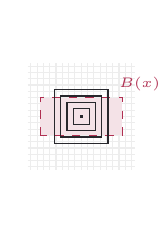
\begin{tikzpicture}
          \useasboundingbox (-0.68,-1.128) rectangle (0.68,1.128);
          \draw[black!7, step=0.08] (-0.68,-0.68) grid (0.68,0.68);
          \fill[accent!14] (-0.52,-0.24) rectangle (0.52,0.24);
          \draw[accent, dashed, thin] (-0.52,-0.24) rectangle (0.52,0.24);
          \node[font=\tiny, text=accent, anchor=south west, inner sep=1pt] at (0.44,0.28) {$B(x)$};
          \draw[ink, thin] (-0.10,-0.10) rectangle (0.10,0.10);
          \draw[ink, thin] (-0.18,-0.18) rectangle (0.18,0.18);
          \draw[ink, thin] (-0.26,-0.26) rectangle (0.26,0.26);
          \draw[ink, thin] (-0.34,-0.34) rectangle (0.34,0.34);
          \fill[ink] (-0.02,-0.02) rectangle (0.02,0.02);
        \end{tikzpicture}\\
        {\tiny\color{soft} four blocks, $+\,2(k{-}1)$ each\par}
      \end{minipage}%
      \begin{minipage}[t]{0.075\linewidth}
        \centering
        \begin{tikzpicture}[baseline=(current bounding box.north)]
          \useasboundingbox (0,0) rectangle (0.55,-4.85);
          \draw[flow] (0,-0.55) -- (0.55,-0.55);
          \draw[flow] (0,-1.66) -- (0.55,-1.66);
          \draw[flow] (0,-2.82) -- (0.55,-2.82);
          \draw[flow] (-0.50,-4.77) -- (1.05,-4.77);
        \end{tikzpicture}
      \end{minipage}%
      \begin{minipage}[t]{0.485\linewidth}
        \centering
        \textbf{The pyramid --- halve, conv.}
        \[
          \begin{gathered}
            r \;=\; 1 + 2(k{-}1)\big(2^{D+1}{-}1\big)\\
            {\color{soft}\scriptstyle 2^{\ell}{\times}\ \text{per station}}\\[5pt]
            m_{\ell} \;=\; 2^{\ell}\,m_{0}\\
            {\color{soft}\scriptstyle \text{width doubles down}}\\[5pt]
            \tfrac{k^{2}m_{\ell}^{2}}{4^{\ell}} \;=\; k^{2}m_{0}^{2}\\
            {\color{soft}\scriptstyle \text{cost per pixel flat}}
          \end{gathered}
        \]
        \begin{tikzpicture}[scale=0.88]
          \useasboundingbox (-1.28,-1.28) rectangle (1.28,1.28);
          \draw[black!7, step=0.08] (-1.28,-1.28) grid (1.28,1.28);
          \fill[accent!14] (-0.52,-0.24) rectangle (0.52,0.24);
          \draw[accent, dashed, thin] (-0.52,-0.24) rectangle (0.52,0.24);
          \draw[ink, thin] (-0.10,-0.10) rectangle (0.10,0.10);
          \draw[ink, thin] (-0.26,-0.26) rectangle (0.26,0.26);
          \draw[ink, thin] (-0.58,-0.58) rectangle (0.58,0.58);
          \draw[ink, thin] (-1.22,-1.22) rectangle (1.22,1.22);
          \fill[ink] (-0.02,-0.02) rectangle (0.02,0.02);
        \end{tikzpicture}\\
        {\tiny\color{soft} four stations, the step doubling\par}
      \end{minipage}
    \end{column}
    \begin{column}{0.375\textwidth}
      \raggedright
      {\scriptsize\color{soft}
       $r$: field side \;$\cdot$\;
       $B$: blocks stacked \;$\cdot$\;
       $m$: width in channels \;$\cdot$\;
       $P$: parameters \;$\cdot$\;
       station $\ell$: the block $\ell$ halvings down, width $m_{\ell}$
       \;$\cdot$\; $D$: deepest station\par}
      \par\smallskip
      \centering
      \begin{tikzpicture}[scale=0.93]
        \draw[-{Stealth[length=1.5mm]}, soft] (0,0) -- (0,4.45);
        \draw[-{Stealth[length=1.5mm]}, soft] (0,0) -- (4.60,0)
          node[anchor=south east, font=\tiny, inner sep=1.5pt] {blocks};
        \node[font=\tiny, text=soft, rotate=90, anchor=south] at (-0.30,2.0)
          {field $r$ [px]};
        \foreach \x/\b in {0.60/2,1.20/4,1.80/6,2.40/8,3.00/10,3.60/12,4.20/14}{
          \draw[soft, thin] (\x,0) -- (\x,-0.05);
          \node[font=\tiny, text=soft, anchor=north] at (\x,-0.06) {\b};}
        \draw[soft, dashed, thin] (0,3.38) -- (4.45,3.38);
        \node[font=\tiny, text=soft, anchor=south west, inner sep=1.5pt] at (0.02,3.39) {$2w_{a}$};
        \draw[ink, semithick] (0,0.065) -- (4.20,3.705);
        \node[font=\tiny, text=ink, anchor=south, inner sep=2pt] at (2.90,2.63) {trunk};
        \fill[good] (0.60,0.585) circle (0.05);
        \node[font=\tiny, text=good, anchor=west, inner sep=2.5pt] at (0.64,0.55) {$9{\times}9$};
        \fill[accent] (2.10,1.885) circle (0.05);
        \node[font=\tiny, text=accent, anchor=north west, inner sep=2pt] at (2.12,1.83) {$29{\times}29$};
        \fill[ink] (3.825,3.38) circle (0.05);
        \node[font=\tiny, text=ink, anchor=north west, inner sep=2.5pt] at (3.72,3.30) {$13$};
        \draw[accent, semithick] (0,0.065) -- (0.30,0.325) -- (0.60,0.845)
          -- (0.90,1.885) -- (1.20,3.965);
        \fill[accent] (0.30,0.325) circle (0.05);
        \fill[accent] (0.60,0.845) circle (0.05);
        \fill[accent] (0.90,1.885) circle (0.05);
        \fill[accent] (1.20,3.965) circle (0.05);
        \node[font=\tiny, text=accent, anchor=west, inner sep=2.5pt] at (1.26,3.965) {$4$ stations};
        \draw[soft, dotted, thin] (0.90,1.885) -- (2.10,1.885);
        \node[font=\tiny, text=soft, anchor=south] at (1.50,1.90) {same $29$};
      \end{tikzpicture}
      \par\smallskip
      \raggedright
      {\scriptsize Encoder stations alone --- the decoder only pushes further.
       Three stations hold the ladder's $29{\times}29$; the fourth passes the
       sweep's reach $2w_{a}$, thirteen full-resolution blocks before the
       trunk does.\par}
    \end{column}
  \end{columns}
\end{frame}

% ---------------------------------------------------------------- 24e Why the U-Net fits
\begin{frame}{One grid per scale --- matching the scales of the interferograms}
  \begin{columns}[c]
    \begin{column}{0.50\textwidth}
      \small
      \textbf{Multi-scale by construction} --- each track pair $(P, S_{n})$
      sees the same relief $z(x)$ at its own fringe rate:
      \par\smallskip
      {\centering
      $\varphi_{n}(x) = \bigl(k_z^{(n)} - k_z^{(P)}\bigr)\, z(x)
        = k_{n}\, z(x), \qquad k_{n} \propto b_{\perp,n}$
      \par}
      \medskip
      {\centering
      \begin{tikzpicture}
        \node[font=\scriptsize, text=soft, anchor=south] at (0.55,0.55) {track pair};
        \node[font=\scriptsize, text=soft, anchor=south] at (2.55,0.55) {its fringes};
        \node[font=\scriptsize, text=soft, anchor=south] at (4.80,0.55) {matching grid};
        \draw[soft, thin] (0.40,0.25) -- (0.40,-3.50);
        \draw[|-|, soft] (0.72,-3.50) -- (0.72,0);
        \node[font=\scriptsize, text=soft, anchor=center] at (1.00,-1.75) {$b_{\perp}$};
        \fill[accent] (0.40,-3.50) circle (0.07);
        \node[font=\scriptsize, text=accent, anchor=north, inner sep=2pt] at (0.40,-3.60) {$P$};
        \fill[ink] (0.40,0) circle (0.06);
        \node[font=\scriptsize, text=soft, anchor=east, inner sep=2pt] at (0.28,0) {$S_{1}$};
        \fill[ink] (0.40,-1.30) circle (0.06);
        \node[font=\scriptsize, text=soft, anchor=east, inner sep=2pt] at (0.28,-1.30) {$S_{2}$};
        \fill[ink] (0.40,-2.60) circle (0.06);
        \node[font=\scriptsize, text=soft, anchor=east, inner sep=2pt] at (0.28,-2.60) {$S_{3}$};
        \fill[black!4] (1.45,-0.35) rectangle (3.65,0.35);
        \foreach \j in {0,...,9}
          \fill[ink!40] (1.45+0.22*\j,-0.35) rectangle ++(0.11,0.70);
        \draw[soft, thin] (1.45,-0.35) rectangle (3.65,0.35);
        \fill[black!4] (1.45,-1.65) rectangle (3.65,-0.95);
        \foreach \j in {0,...,4}
          \fill[ink!40] (1.45+0.44*\j,-1.65) rectangle ++(0.22,0.70);
        \draw[soft, thin] (1.45,-1.65) rectangle (3.65,-0.95);
        \fill[black!4] (1.45,-2.95) rectangle (3.65,-2.25);
        \fill[ink!40] (1.45,-2.95) rectangle ++(0.88,0.70);
        \fill[ink!40] (3.21,-2.95) rectangle (3.65,-2.25);
        \draw[soft, thin] (1.45,-2.95) rectangle (3.65,-2.25);
        \draw[-{Stealth[length=1.5mm]}, soft] (3.78,0) -- (4.10,0);
        \draw[-{Stealth[length=1.5mm]}, soft] (3.78,-1.30) -- (4.10,-1.30);
        \draw[-{Stealth[length=1.5mm]}, soft] (3.78,-2.60) -- (4.10,-2.60);
        \begin{scope}[shift={(4.20,-0.40)}]
          \draw[ink!20, step=0.05] (0,0) grid (1.20,0.80);
          \draw[soft, thin] (0,0) rectangle (1.20,0.80);
        \end{scope}
        \begin{scope}[shift={(4.20,-1.70)}]
          \draw[ink!30, step=0.10] (0,0) grid (1.20,0.80);
          \draw[soft, thin] (0,0) rectangle (1.20,0.80);
        \end{scope}
        \begin{scope}[shift={(4.20,-3.00)}]
          \draw[ink!30, step=0.40] (0,0) grid (1.20,0.80);
          \draw[soft, thin] (0,0) rectangle (1.20,0.80);
        \end{scope}
        \node[font=\scriptsize, text=soft, anchor=north] at (4.80,-0.45) {scale 0};
        \node[font=\scriptsize, text=soft, anchor=north] at (4.80,-1.75) {scale 1};
        \node[font=\scriptsize, text=soft, anchor=north] at (4.80,-3.05) {scale 3};
      \end{tikzpicture}
      \par}
    \end{column}
    \begin{column}{0.46\textwidth}
      \centering
      \begin{tikzpicture}[scale=0.85]
        \node[font=\scriptsize, text=ink, anchor=south] at (0.80,1.32) {U-Net};
        \node[font=\scriptsize, text=ink, anchor=south] at (3.25,1.32) {local CNN};
        \begin{scope}
          \fill[argA!30] (0.40,0.40) rectangle (1.20,0.80);
          \draw[ink!20, step=0.05] (0,0) grid (1.60,1.20);
          \draw[accent, dashed, thin] (0.40,0.40) rectangle (1.20,0.80);
          \draw[soft, thin] (0,0) rectangle (1.60,1.20);
          \node[font=\tiny, text=accent, anchor=south west, inner sep=1pt] at (0.36,0.84) {$B(x)$};
        \end{scope}
        \begin{scope}[shift={(0,-1.70)}]
          \fill[argA!30] (0.40,0.40) rectangle (1.20,0.80);
          \draw[ink!30, step=0.10] (0,0) grid (1.60,1.20);
          \draw[accent, dashed, thin] (0.40,0.40) rectangle (1.20,0.80);
          \draw[soft, thin] (0,0) rectangle (1.60,1.20);
        \end{scope}
        \begin{scope}[shift={(0,-3.40)}]
          \fill[argA!30] (0.40,0.40) rectangle (1.20,0.80);
          \draw[ink!30, step=0.20] (0,0) grid (1.60,1.20);
          \draw[accent, dashed, thin] (0.40,0.40) rectangle (1.20,0.80);
          \draw[soft, thin] (0,0) rectangle (1.60,1.20);
        \end{scope}
        \begin{scope}[shift={(0,-5.10)}]
          \fill[argA!30] (0.40,0.40) rectangle (1.20,0.80);
          \draw[ink!30, step=0.40] (0,0) grid (1.60,1.20);
          \draw[accent, dashed, thin] (0.40,0.40) rectangle (1.20,0.80);
          \draw[soft, thin] (0,0) rectangle (1.60,1.20);
        \end{scope}
        \node[font=\tiny, text=soft, anchor=east, align=right, inner sep=2pt] at (-0.08,0.60) {scale 0\\a value per pixel};
        \node[font=\tiny, text=soft, anchor=east, align=right, inner sep=2pt] at (-0.08,-1.10) {scale 1};
        \node[font=\tiny, text=soft, anchor=east, align=right, inner sep=2pt] at (-0.08,-2.80) {scale 2};
        \node[font=\tiny, text=soft, anchor=east, align=right, inner sep=2pt] at (-0.08,-4.50) {scale 3\\two cells};
        \draw[-{Stealth[length=1.5mm]}, soft] (0.80,0) -- (0.80,-0.50);
        \node[font=\tiny, text=soft, anchor=west, inner sep=2pt] at (0.92,-0.25) {$\div 4$};
        \draw[-{Stealth[length=1.5mm]}, soft] (0.80,-1.70) -- (0.80,-2.20);
        \node[font=\tiny, text=soft, anchor=west, inner sep=2pt] at (0.92,-1.95) {$\div 4$};
        \draw[-{Stealth[length=1.5mm]}, soft] (0.80,-3.40) -- (0.80,-3.90);
        \node[font=\tiny, text=soft, anchor=west, inner sep=2pt] at (0.92,-3.65) {$\div 4$};
        \begin{scope}[shift={(2.45,0)}]
          \fill[argA!30] (0.40,0.40) rectangle (1.20,0.80);
          \draw[ink!20, step=0.05] (0,0) grid (1.60,1.20);
          \draw[accent, dashed, thin] (0.40,0.40) rectangle (1.20,0.80);
          \draw[soft, thin] (0,0) rectangle (1.60,1.20);
        \end{scope}
        \begin{scope}[shift={(2.45,-1.70)}]
          \fill[argA!30] (0.40,0.40) rectangle (1.20,0.80);
          \draw[ink!20, step=0.05] (0,0) grid (1.60,1.20);
          \draw[accent, dashed, thin] (0.40,0.40) rectangle (1.20,0.80);
          \draw[soft, thin] (0,0) rectangle (1.60,1.20);
        \end{scope}
        \begin{scope}[shift={(2.45,-3.40)}]
          \fill[argA!30] (0.40,0.40) rectangle (1.20,0.80);
          \draw[ink!20, step=0.05] (0,0) grid (1.60,1.20);
          \draw[accent, dashed, thin] (0.40,0.40) rectangle (1.20,0.80);
          \draw[soft, thin] (0,0) rectangle (1.60,1.20);
        \end{scope}
        \begin{scope}[shift={(2.45,-5.10)}]
          \fill[argA!30] (0.40,0.40) rectangle (1.20,0.80);
          \draw[ink!20, step=0.05] (0,0) grid (1.60,1.20);
          \draw[accent, dashed, thin] (0.40,0.40) rectangle (1.20,0.80);
          \draw[soft, thin] (0,0) rectangle (1.60,1.20);
          \fill[accent] (0.80,0.60) rectangle (0.85,0.65);
          \node[font=\tiny, text=accent, anchor=north, inner sep=2pt] at (0.82,0.58) {$x$};
        \end{scope}
        \node[font=\tiny, text=soft, anchor=north] at (3.25,-5.15) {scale 0 --- unchanged};
        \draw[-{Stealth[length=1.5mm]}, soft] (3.25,0) -- (3.25,-0.50);
        \node[font=\tiny, text=soft, anchor=west, inner sep=2pt] at (3.37,-0.25) {$\times 1$};
        \draw[-{Stealth[length=1.5mm]}, soft] (3.25,-1.70) -- (3.25,-2.20);
        \node[font=\tiny, text=soft, anchor=west, inner sep=2pt] at (3.37,-1.95) {$\times 1$};
        \draw[-{Stealth[length=1.5mm]}, soft] (3.25,-3.40) -- (3.25,-3.90);
        \node[font=\tiny, text=soft, anchor=west, inner sep=2pt] at (3.37,-3.65) {$\times 1$};
        \draw[-{Stealth[length=1.5mm]}, soft] (4.10,-4.50) -- (4.35,-4.50);
        \foreach \i in {0,1,2,3,4,5,6,7}
          \draw[soft, thin, fill=accent!10] (4.40,-4.96+0.115*\i) rectangle (4.90,-4.845+0.115*\i);
        \node[font=\tiny, text=soft, anchor=north, align=center, inner sep=2pt] at (4.65,-5.02)
          {$m$ channels\\at $x$};
      \end{tikzpicture}
    \end{column}
  \end{columns}
\end{frame}

% ---------------------------------------------------------------- 25 Input ablation: the test
\begin{frame}{Input ablation --- which channels, and how many tracks?}
  \begin{columns}[c]
    \begin{column}{0.43\textwidth}
      \centering
      \begin{tikzpicture}
        \node[font=\tiny\bfseries,text=soft] at (1.15,5.75) {reduced --- 5 tracks};
        \node[font=\tiny\bfseries,text=soft] at (3.75,5.75) {all --- 29 tracks};
        \node[font=\tiny\bfseries,text=soft,rotate=90] at (-0.35,4.675) {$|A|$ only};
        \node[font=\tiny\bfseries,text=soft,rotate=90] at (-0.35,2.725) {$\varphi$ only};
        \node[font=\tiny\bfseries,text=soft,rotate=90] at (-0.35,0.775) {$|A|+\varphi$};
        % row 1: amplitude only
        \begin{scope}[shift={(0,3.9)}]
          \draw[soft,thin,rounded corners=2pt,fill=black!2] (0,0) rectangle (2.3,1.55);
          \foreach \i in {3,2,1} \draw[soft,thin,fill=black!2] (0.3+0.05*\i,0.65+0.05*\i) rectangle ++(0.6,0.6);
          \draw[soft,thin,fill=white] (0.3,0.65) rectangle ++(0.6,0.6);
          \draw[black!8,step=0.15,shift={(0.3,0.65)}] (0,0) grid (0.6,0.6);
          \draw[soft,thin,fill=white] (1.3,0.65) rectangle ++(0.6,0.6);
          \begin{scope} \clip (1.3,0.65) rectangle ++(0.6,0.6); \foreach \r in {0.3,0.42,...,1.3} \draw[black!12,thin] (2.05,0.4) circle (\r); \end{scope}
          \draw[accent,thick] (1.3,0.65) -- ++(0.6,0.6);
          \draw[accent,thick] (1.3,1.25) -- ++(0.6,-0.6);
          \node[font=\tiny,text=soft,anchor=north] at (1.15,0.47) {5 $|A|$, no $\varphi$};
        \end{scope}
        \begin{scope}[shift={(2.6,3.9)}]
          \draw[soft,thin,rounded corners=2pt,fill=black!2] (0,0) rectangle (2.3,1.55);
          \foreach \i in {6,5,4,3,2,1} \draw[soft,thin,fill=black!2] (0.3+0.05*\i,0.57+0.05*\i) rectangle ++(0.6,0.6);
          \draw[soft,thin,fill=white] (0.3,0.57) rectangle ++(0.6,0.6);
          \draw[black!8,step=0.15,shift={(0.3,0.57)}] (0,0) grid (0.6,0.6);
          \draw[soft,thin,fill=white] (1.3,0.65) rectangle ++(0.6,0.6);
          \begin{scope} \clip (1.3,0.65) rectangle ++(0.6,0.6); \foreach \r in {0.3,0.42,...,1.3} \draw[black!12,thin] (2.05,0.4) circle (\r); \end{scope}
          \draw[accent,thick] (1.3,0.65) -- ++(0.6,0.6);
          \draw[accent,thick] (1.3,1.25) -- ++(0.6,-0.6);
          \node[font=\tiny,text=soft,anchor=north] at (1.15,0.47) {29 $|A|$, no $\varphi$};
        \end{scope}
        % row 2: phase only
        \begin{scope}[shift={(0,1.95)}]
          \draw[soft,thin,rounded corners=2pt,fill=black!2] (0,0) rectangle (2.3,1.55);
          \draw[soft,thin,fill=white] (0.3,0.65) rectangle ++(0.6,0.6);
          \draw[black!8,step=0.15,shift={(0.3,0.65)}] (0,0) grid (0.6,0.6);
          \draw[accent,thick] (0.3,0.65) -- ++(0.6,0.6);
          \draw[accent,thick] (0.3,1.25) -- ++(0.6,-0.6);
          \foreach \i in {3,2,1} \draw[soft,thin,fill=black!2] (1.3+0.05*\i,0.65+0.05*\i) rectangle ++(0.6,0.6);
          \draw[soft,thin,fill=white] (1.3,0.65) rectangle ++(0.6,0.6);
          \begin{scope} \clip (1.3,0.65) rectangle ++(0.6,0.6); \foreach \r in {0.3,0.42,...,1.3} \draw[accent!30,thin] (2.05,0.4) circle (\r); \end{scope}
          \node[font=\tiny,text=soft,anchor=north] at (1.15,0.47) {4 $\varphi$, no $|A|$};
        \end{scope}
        \begin{scope}[shift={(2.6,1.95)}]
          \draw[soft,thin,rounded corners=2pt,fill=black!2] (0,0) rectangle (2.3,1.55);
          \draw[soft,thin,fill=white] (0.3,0.65) rectangle ++(0.6,0.6);
          \draw[black!8,step=0.15,shift={(0.3,0.65)}] (0,0) grid (0.6,0.6);
          \draw[accent,thick] (0.3,0.65) -- ++(0.6,0.6);
          \draw[accent,thick] (0.3,1.25) -- ++(0.6,-0.6);
          \foreach \i in {6,5,4,3,2,1} \draw[soft,thin,fill=black!2] (1.3+0.05*\i,0.57+0.05*\i) rectangle ++(0.6,0.6);
          \draw[soft,thin,fill=white] (1.3,0.57) rectangle ++(0.6,0.6);
          \begin{scope} \clip (1.3,0.57) rectangle ++(0.6,0.6); \foreach \r in {0.3,0.42,...,1.3} \draw[accent!30,thin] (2.05,0.32) circle (\r); \end{scope}
          \node[font=\tiny,text=soft,anchor=north] at (1.15,0.47) {28 $\varphi$, no $|A|$};
        \end{scope}
        % row 3: both
        \begin{scope}[shift={(0,0)}]
          \draw[accent!60,thin,rounded corners=2pt,fill=accent!4] (0,0) rectangle (2.3,1.55);
          \foreach \i in {3,2,1} \draw[soft,thin,fill=black!2] (0.3+0.05*\i,0.65+0.05*\i) rectangle ++(0.6,0.6);
          \draw[soft,thin,fill=white] (0.3,0.65) rectangle ++(0.6,0.6);
          \draw[black!8,step=0.15,shift={(0.3,0.65)}] (0,0) grid (0.6,0.6);
          \foreach \i in {3,2,1} \draw[soft,thin,fill=black!2] (1.3+0.05*\i,0.65+0.05*\i) rectangle ++(0.6,0.6);
          \draw[soft,thin,fill=white] (1.3,0.65) rectangle ++(0.6,0.6);
          \begin{scope} \clip (1.3,0.65) rectangle ++(0.6,0.6); \foreach \r in {0.3,0.42,...,1.3} \draw[accent!30,thin] (2.05,0.4) circle (\r); \end{scope}
          \node[font=\tiny,text=soft,anchor=north] at (1.15,0.47) {5 $|A|$ + 4 $\varphi$};
          \node[font=\tiny,text=accent,anchor=north] at (1.15,-0.06) {reference (reduced stack)};
        \end{scope}
        \begin{scope}[shift={(2.6,0)}]
          \draw[soft,thin,rounded corners=2pt,fill=black!2] (0,0) rectangle (2.3,1.55);
          \foreach \i in {6,5,4,3,2,1} \draw[soft,thin,fill=black!2] (0.3+0.05*\i,0.57+0.05*\i) rectangle ++(0.6,0.6);
          \draw[soft,thin,fill=white] (0.3,0.57) rectangle ++(0.6,0.6);
          \draw[black!8,step=0.15,shift={(0.3,0.57)}] (0,0) grid (0.6,0.6);
          \foreach \i in {6,5,4,3,2,1} \draw[soft,thin,fill=black!2] (1.3+0.05*\i,0.57+0.05*\i) rectangle ++(0.6,0.6);
          \draw[soft,thin,fill=white] (1.3,0.57) rectangle ++(0.6,0.6);
          \begin{scope} \clip (1.3,0.57) rectangle ++(0.6,0.6); \foreach \r in {0.3,0.42,...,1.3} \draw[accent!30,thin] (2.05,0.32) circle (\r); \end{scope}
          \node[font=\tiny,text=soft,anchor=north] at (1.15,0.47) {29 $|A|$ + 28 $\varphi$};
          \node[font=\tiny,text=soft,anchor=north] at (1.15,-0.06) {full stack};
        \end{scope}
      \end{tikzpicture}
    \end{column}
    \begin{column}{0.54\textwidth}
      \small
      Theory says the elevation information lives in the \textbf{interferogram
      phase}: amplitudes alone should not determine the profile. But the context
      ladder just showed the network leans on spatial structure --- so two axes,
      crossed:
      \par\smallskip
      \begin{itemize}\setlength{\itemsep}{3pt}
        \item \textbf{The grid}: \emph{which channels} ($|A|$ only / $\varphi$
              only / both) $\times$ \emph{how many tracks} (the reduced 5-track
              selection / all 29). Six retrains of the reference U-Net --- same
              $K{=}2$ target, loss and split, only the input stack changes.
        \item \textbf{H1 --- phase is everything}: strip the phase and
              reconstruction collapses toward nothing usable; amplitude
              diversity cannot buy it back.
        \item \textbf{H2 --- priors carry part of it}: amplitude-only lands in
              between, and 29 $|A|$ closes part of the gap to the reference.
        \item \textbf{H3 --- tracks pay everywhere}: if tracks are information,
              every modality should improve reduced $\to$ all; the open question
              is whether diversity can \emph{substitute} for a missing modality.
      \end{itemize}
    \end{column}
  \end{columns}
\end{frame}

% ---------------------------------------------------------------- 25b Input ablation: the verdict
\begin{frame}{The verdict --- every channel pays on the curve, phase still places the scatterers}
    \centering
  \scriptsize
  \renewcommand{\arraystretch}{0.98}
  \setlength{\tabcolsep}{2.5pt}
  \renewcommand{\seedtag}{ctxA}
  \begin{tabular}{@{}l cc cc !{\hspace{3pt}} cc@{}}
    \toprule
    & \multicolumn{2}{c}{$|A|$ only} & \multicolumn{2}{c}{$\varphi$ only} & \multicolumn{2}{c@{}}{$|A|+\varphi$} \\
    \cmidrule(lr){2-3}\cmidrule(lr){4-5}\cmidrule(l){6-7}
    metric & red. & all & red. & all & red. & all \\
    \midrule
    \multicolumn{7}{@{}l}{\emph{training (validation)}} \\
    val loss $\downarrow$ & \seedpm{0.179}{.001} & \seedpm{0.164}{.002} & \seedpm{0.162}{.001} & \seedpm{0.137}{.002} & \seedpm{0.142}{.001} & \seedpm{\hlval{good}{\textbf{0.122}}}{.000} \\
    \addlinespace
    \multicolumn{7}{@{}l}{\emph{reconstruction (curve)}} \\
    curve $R^2$ $\uparrow$ & \seedpm{0.369}{.014} & \seedpm{0.437}{.010} & \seedpm{0.409}{.018} & \seedpm{0.503}{.007} & \seedpm{0.569}{.008} & \seedpm{\hlval{good}{\textbf{0.667}}}{.015} \\
    curve MAE $\downarrow$ & \seedpm{0.066}{.001} & \seedpm{0.060}{.001} & \seedpm{0.059}{.002} & \seedpm{0.051}{.001} & \seedpm{0.050}{.001} & \seedpm{\textbf{0.043}}{.001} \\
    PSNR [dB] $\uparrow$  & \seedpm{48.7}{.1} & \seedpm{49.2}{.1} & \seedpm{48.9}{.1} & \seedpm{49.7}{.1} & \seedpm{50.3}{.1} & \seedpm{\textbf{51.4}}{.2} \\
    SSIM elev $\uparrow$  & \seedpm{0.946}{.001} & \seedpm{0.951}{.001} & \seedpm{0.952}{.001} & \seedpm{0.959}{.001} & \seedpm{0.959}{.001} & \seedpm{0.963}{.001} \\
    SSIM range $\uparrow$ & \seedpm{0.901}{.001} & \seedpm{0.911}{.002} & \seedpm{0.916}{.002} & \seedpm{0.927}{.002} & \seedpm{0.926}{.002} & \seedpm{0.933}{.001} \\
    SSIM azim $\uparrow$  & \seedpm{0.925}{.000} & \seedpm{0.933}{.001} & \seedpm{0.936}{.002} & \seedpm{0.946}{.001} & \seedpm{0.946}{.001} & \seedpm{0.953}{.001} \\
    profile cos med\,$\uparrow$ & \seedpm{0.665}{.020} & \seedpm{0.737}{.017} & \seedpm{0.912}{.012} & \seedpm{\textbf{0.931}}{.009} & \seedpm{0.850}{.024} & \seedpm{0.890}{.012} \\
    \addlinespace
    \multicolumn{7}{@{}l}{\emph{detection (matched)}} \\
    precision $\uparrow$   & \seedpm{0.758}{.008} & \seedpm{0.785}{.009} & \seedpm{0.830}{.007} & \seedpm{\textbf{0.853}}{.008} & \seedpm{0.821}{.008} & \seedpm{0.839}{.005} \\
    recall $\uparrow$      & \seedpm{0.652}{.027} & \seedpm{0.679}{.028} & \seedpm{\hlval{good}{\textbf{0.817}}}{.021} & \seedpm{0.765}{.038} & \seedpm{0.641}{.029} & \seedpm{\hlval{accent}{0.636}}{.024} \\
    matched F1 $\uparrow$  & \seedpm{0.701}{.019} & \seedpm{0.728}{.020} & \seedpm{\hlval{good}{\textbf{0.823}}}{.012} & \seedpm{0.806}{.024} & \seedpm{0.720}{.020} & \seedpm{0.723}{.017} \\
    count exact $\uparrow$ & \seedpm{0.609}{.034} & \seedpm{0.633}{.035} & \seedpm{\hlval{good}{\textbf{0.802}}}{.029} & \seedpm{0.741}{.048} & \seedpm{0.595}{.034} & \seedpm{0.591}{.033} \\
    peak err med $\downarrow$ & \seedpm{1.48}{.30} & \seedpm{1.34}{.00} & \seedpm{\textbf{0.67}}{.00} & \seedpm{\textbf{0.67}}{.00} & \seedpm{0.81}{.30} & \seedpm{0.81}{.30} \\
    peak err p95 $\downarrow$ & \seedpm{15.6}{.3} & \seedpm{15.3}{.3} & \seedpm{\textbf{11.7}}{1.9} & \seedpm{14.0}{.3} & \seedpm{15.4}{.5} & \seedpm{15.2}{.4} \\
    \bottomrule
  \end{tabular}
  \par\vspace{3pt}
  \parbox{0.82\textwidth}{\tiny\color{soft} \textbf{runs}: UNet $\cdot$ conv $\cdot$ sorted-GT $\cdot$ $K{=}2$ $\cdot$ param-MSE $\cdot$ presence none $\cdot$ full norm ladder $\cdot$ hv flips $\cdot$ patch $64{\times}32$ (input = column); five seeded replicas per arm, cells mean $\pm$ seed std; held-out test, $5.0$\,M px. red.\ $=$ 5 tracks (5 $|A|$ / 4 $\varphi$); all $=$ 29 tracks (29 $|A|$ / 28 $\varphi$). \textbf{bold} $=$ best in row, marked only where best and worst differ by more than $5\%$; \textcolor{good}{green} $=$ the full-stack curve peak and the phase detection wins, \textcolor{accent}{red} $=$ amplitude diluting recall; matched $=$ Hungarian pairing. Peak err med/p95: per-pixel peak-error distribution; profile cos med: median per-pixel cosine to the GT profile.\par}
    

\end{frame}

% ---------------------------------------------------------------- 25c Input ablation by scatterer count
\begin{frame}{Input ablation by scatterer count --- each parameter reads its own modality}
    \centering
  \scriptsize
  \renewcommand{\arraystretch}{1.04}
  \setlength{\tabcolsep}{2.5pt}
  \renewcommand{\seedtag}{ctxB}
  \begin{tabular}{@{}l cc cc !{\hspace{3pt}} cc@{}}
    \toprule
    & \multicolumn{2}{c}{$|A|$ only} & \multicolumn{2}{c}{$\varphi$ only} & \multicolumn{2}{c@{}}{$|A|+\varphi$} \\
    \cmidrule(lr){2-3}\cmidrule(lr){4-5}\cmidrule(l){6-7}
    metric & red. & all & red. & all & red. & all \\
    \midrule
    matched precision $\uparrow$ & \seedpm{0.758}{.008} & \seedpm{0.785}{.009} & \seedpm{0.830}{.007} & \seedpm{\textbf{0.853}}{.008} & \seedpm{0.821}{.008} & \seedpm{0.839}{.005} \\
    \quad $k{=}1$                & \seedpm{0.803}{.012} & \seedpm{0.821}{.011} & \seedpm{0.875}{.007} & \seedpm{\textbf{0.890}}{.009} & \seedpm{0.853}{.008} & \seedpm{0.867}{.011} \\
    \quad $k{=}2$                & \seedpm{0.696}{.009} & \seedpm{0.734}{.009} & \seedpm{0.761}{.012} & \seedpm{0.803}{.008} & \seedpm{0.782}{.007} & \seedpm{\textbf{0.806}}{.007} \\
    \addlinespace
    matched recall $\uparrow$    & \seedpm{0.652}{.027} & \seedpm{0.679}{.028} & \seedpm{\hlval{good}{\textbf{0.817}}}{.021} & \seedpm{0.765}{.038} & \seedpm{0.641}{.029} & \seedpm{\hlval{accent}{0.636}}{.024} \\
    \quad $k{=}1$                & \seedpm{0.684}{.046} & \seedpm{0.704}{.047} & \seedpm{\hlval{good}{\textbf{0.882}}}{.040} & \seedpm{0.779}{.065} & \seedpm{0.620}{.046} & \seedpm{0.593}{.043} \\
    \quad $k{=}2$                & \seedpm{0.606}{.009} & \seedpm{0.643}{.007} & \seedpm{0.725}{.009} & \seedpm{\hlval{good}{\textbf{0.745}}}{.003} & \seedpm{0.672}{.008} & \seedpm{0.698}{.008} \\
    \addlinespace
    count acc\,$\mid$\,pred $k{=}1$\,$\uparrow$ & \seedpm{0.961}{.004} & \seedpm{0.963}{.004} & \seedpm{0.969}{.005} & \seedpm{0.964}{.003} & \seedpm{0.948}{.007} & \seedpm{0.959}{.002} \\
    count acc\,$\mid$\,pred $k{=}2$\,$\uparrow$ & \seedpm{0.646}{.003} & \seedpm{0.665}{.007} & \seedpm{0.724}{.007} & \seedpm{\hlval{good}{\textbf{0.770}}}{.005} & \seedpm{0.733}{.010} & \seedpm{0.767}{.007} \\
    \addlinespace
    matched $\mu$ MAE $\downarrow$ & \seedpm{2.95}{.09} & \seedpm{2.65}{.08} & \seedpm{2.29}{.08} & \seedpm{\textbf{2.04}}{.12} & \seedpm{2.30}{.08} & \seedpm{2.15}{.06} \\
    \quad $k{=}1$                & \seedpm{1.25}{.05} & \seedpm{1.03}{.04} & \seedpm{0.55}{.05} & \seedpm{\hlval{good}{\textbf{0.51}}}{.02} & \seedpm{0.59}{.04} & \seedpm{0.52}{.02} \\
    \addlinespace[2pt]
    \quad $k{=}2$                & \seedpm{4.88}{.08} & \seedpm{4.52}{.06} & \seedpm{4.58}{.15} & \seedpm{3.86}{.12} & \seedpm{4.05}{.08} & \seedpm{\textbf{3.74}}{.06} \\
    \addlinespace
    matched $\sigma$ MAE $\downarrow$ & \seedpm{0.97}{.03} & \seedpm{0.91}{.03} & \seedpm{0.89}{.04} & \seedpm{\textbf{0.79}}{.05} & \seedpm{0.87}{.03} & \seedpm{0.80}{.03} \\
    \quad $k{=}1$                & \seedpm{0.29}{.02} & \seedpm{0.26}{.01} & \seedpm{0.24}{.01} & \seedpm{\textbf{0.20}}{.01} & \seedpm{0.25}{.01} & \seedpm{0.21}{.01} \\
    \quad $k{=}2$                & \seedpm{1.74}{.01} & \seedpm{1.64}{.01} & \seedpm{1.76}{.05} & \seedpm{1.51}{.05} & \seedpm{1.51}{.01} & \seedpm{\textbf{1.38}}{.01} \\
    \addlinespace
    matched $a$ MAE $\downarrow$ & \seedpm{0.369}{.017} & \seedpm{0.356}{.015} & \seedpm{\hlval{accent}{0.464}}{.009} & \seedpm{\hlval{accent}{0.446}}{.025} & \seedpm{0.374}{.026} & \seedpm{\textbf{0.346}}{.012} \\
    \quad $k{=}1$                & \seedpm{0.164}{.015} & \seedpm{\textbf{0.161}}{.010} & \seedpm{0.233}{.010} & \seedpm{0.234}{.021} & \seedpm{\textbf{0.161}}{.017} & \seedpm{0.165}{.016} \\
    \quad $k{=}2$                & \seedpm{0.601}{.007} & \seedpm{0.579}{.027} & \seedpm{0.771}{.013} & \seedpm{0.698}{.011} & \seedpm{0.593}{.022} & \seedpm{\textbf{0.524}}{.007} \\
    \bottomrule
  \end{tabular}
  \par\vspace{3pt}
  \parbox{0.82\textwidth}{\tiny\color{soft} \textbf{runs}: UNet $\cdot$ conv $\cdot$ sorted-GT $\cdot$ $K{=}2$ $\cdot$ param-MSE $\cdot$ presence none $\cdot$ full norm ladder $\cdot$ hv flips $\cdot$ patch $64{\times}32$ (input = column); held-out test, cells mean $\pm$ seed std over five seeded replicas; $k$ $=$ true scatterer count of the pixel. red.\ $=$ 5 tracks, all $=$ 29 tracks. \textbf{bold} $=$ best in row, marked only where best and worst differ by more than $5\%$; \textcolor{good}{green} $=$ detection and position living in the phase, \textcolor{accent}{red} $=$ amplitude error without the $|A|$ channels. Precision rewards under-prediction --- rank on recall. count acc $\mid$ pred $k$: share of pixels claiming exactly $k$ scatterers whose true count is $k$. $\mu$, $\sigma$ in elevation units; $a$ in linear amplitude.\par}
    

\end{frame}

% ---------------------------------------------------------------- 25d Input ablation: predicted stats vs GT
\begin{frame}{Input ablation, predicted statistics vs the GT --- phase fires the slots, the full stack calibrates layover}
    \centering
  \scriptsize
  \renewcommand{\arraystretch}{0.90}
  \setlength{\tabcolsep}{2.5pt}
  \renewcommand{\seedtag}{ctxC}
  \begin{tabular}{@{}l !{\color{white}\vrule width 1.2pt} c !{\color{white}\vrule width 1.2pt} cc cc !{\hspace{1pt}} cc@{}}
    \toprule
    & & \multicolumn{2}{c}{$|A|$ only} & \multicolumn{2}{c}{$\varphi$ only} & \multicolumn{2}{c@{}}{$|A|+\varphi$} \\
    \cmidrule(lr){3-4}\cmidrule(lr){5-6}\cmidrule(l){7-8}
    prediction mean & \textcolor{good}{GT} & red. & all & red. & all & red. & all \\
    \midrule
    \multicolumn{8}{@{}l}{\textcolor{soft}{\emph{slot 0 --- strongest scatterer; GT-active on every pixel}}} \\
    \quad active frac         & 1.00    & \seedpm{0.74}{.03} & \seedpm{0.75}{.04} & \seedpm{\hlval{good}{\textbf{0.90}}}{.03} & \seedpm{0.82}{.05} & \seedpm{0.69}{.03} & \seedpm{0.67}{.03} \\
    \quad $a$ --- active      & 0.77    & \seedpm{0.85}{.03} & \seedpm{0.83}{.04} & \seedpm{0.71}{.04} & \seedpm{\textbf{0.72}}{.02} & \seedpm{0.90}{.03} & \seedpm{0.92}{.04} \\
    \quad $\mu$ --- active    & $-4.89$ & \seedpm{$-4.03$}{.10} & \seedpm{$-4.15$}{.17} & \seedpm{$-4.29$}{.05} & \seedpm{\textbf{$-4.52$}}{.08} & \seedpm{$-3.92$}{.10} & \seedpm{$-4.16$}{.09} \\
    \quad $\sigma$ --- active & 1.76    & \seedpm{1.49}{.04} & \seedpm{1.50}{.03} & \seedpm{1.41}{.05} & \seedpm{1.59}{.06} & \seedpm{1.48}{.05} & \seedpm{\textbf{1.65}}{.04} \\
    \addlinespace[1.5pt]
    \multicolumn{8}{@{}l}{\textcolor{soft}{\emph{slot 1 --- second scatterer; GT-active on 26\% of pixels}}} \\
    \quad active frac         & 0.260 & \seedpm{0.346}{.003} & \seedpm{0.338}{.006} & \seedpm{0.338}{.006} & \seedpm{0.308}{.004} & \seedpm{0.299}{.006} & \seedpm{\hlval{good}{\textbf{0.289}}}{.004} \\
    \quad $a$ --- active      & 1.43  & \seedpm{1.05}{.02} & \seedpm{1.08}{.05} & \seedpm{1.05}{.05} & \seedpm{1.08}{.03} & \seedpm{1.04}{.03} & \seedpm{\hlval{good}{\textbf{1.15}}}{.01} \\
    \quad $a$ --- inact.      & 0.00  & \seedpm{0.68}{.01} & \seedpm{0.64}{.03} & \seedpm{0.44}{.04} & \seedpm{0.48}{.01} & \seedpm{\textbf{0.42}}{.01} & \seedpm{0.49}{.03} \\
    \quad $\mu$ --- active    & 11.34 & \seedpm{9.73}{.46} & \seedpm{9.60}{.61} & \seedpm{10.20}{.14} & \seedpm{10.25}{.51} & \seedpm{10.09}{.33} & \seedpm{\hlval{good}{\textbf{10.79}}}{.29} \\
    \quad $\mu$ --- inact.    & ---   & \seedpm{4.04}{.38} & \seedpm{2.72}{.33} & \seedpm{3.51}{.35} & \seedpm{2.55}{.28} & \seedpm{4.09}{.31} & \seedpm{3.71}{.21} \\
    \quad $\sigma$ --- active & 3.53  & \seedpm{3.10}{.03} & \seedpm{3.12}{.05} & \seedpm{2.99}{.02} & \seedpm{3.11}{.05} & \seedpm{2.94}{.05} & \seedpm{\hlval{good}{\textbf{3.18}}}{.03} \\
    \quad $\sigma$ --- inact. & ---   & \seedpm{2.47}{.02} & \seedpm{2.19}{.04} & \seedpm{1.91}{.02} & \seedpm{1.86}{.02} & \seedpm{1.87}{.03} & \seedpm{1.81}{.02} \\
    \addlinespace[1.5pt]
    \multicolumn{8}{@{}l}{\textcolor{soft}{\emph{distribution width --- std over GT-active pixels}}} \\
    \quad $a$ --- slot 0      & 1.48  & \seedpm{1.15}{.02} & \seedpm{1.16}{.05} & \seedpm{1.00}{.06} & \seedpm{1.00}{.02} & \seedpm{1.17}{.03} & \seedpm{\textbf{1.19}}{.01} \\
    \quad $\mu$ --- slot 0    & 3.30  & \seedpm{1.73}{.08} & \seedpm{1.91}{.07} & \seedpm{2.11}{.07} & \seedpm{\textbf{2.33}}{.10} & \seedpm{1.99}{.07} & \seedpm{2.24}{.07} \\
    \quad $\sigma$ --- slot 0 & 2.84  & \seedpm{0.83}{.01} & \seedpm{0.91}{.02} & \seedpm{1.01}{.05} & \seedpm{\textbf{1.35}}{.07} & \seedpm{0.95}{.03} & \seedpm{1.28}{.01} \\
    \quad $a$ --- slot 1      & 1.45  & \seedpm{0.77}{.02} & \seedpm{0.83}{.05} & \seedpm{0.86}{.04} & \seedpm{0.87}{.02} & \seedpm{0.83}{.04} & \seedpm{\textbf{0.89}}{.01} \\
    \quad $\mu$ --- slot 1    & 16.24 & \seedpm{7.14}{.29} & \seedpm{7.74}{.36} & \seedpm{9.37}{.31} & \seedpm{\textbf{10.90}}{.75} & \seedpm{8.72}{.18} & \seedpm{10.06}{.27} \\
    \quad $\sigma$ --- slot 1 & 4.01  & \seedpm{0.80}{.03} & \seedpm{0.92}{.04} & \seedpm{1.08}{.02} & \seedpm{1.33}{.04} & \seedpm{1.07}{.02} & \seedpm{\textbf{1.34}}{.03} \\
    \bottomrule
  \end{tabular}
  \par\vspace{3pt}
  \parbox{0.82\textwidth}{\tiny\color{soft} \textbf{runs}: UNet $\cdot$ conv $\cdot$ sorted-GT $\cdot$ $K{=}2$ $\cdot$ param-MSE $\cdot$ presence none $\cdot$ full norm ladder $\cdot$ hv flips $\cdot$ patch $64{\times}32$ (input = column); five seeded replicas per arm, cells mean $\pm$ seed std; means conditioned on the slot's GT activity mask. red.\ $=$ 5 tracks, all $=$ 29 tracks. \textbf{bold} $=$ closest to the \textcolor{good}{GT} column, marked only where best and worst differ by more than $5\%$; \textcolor{good}{green} $=$ phase firing the slots and the full-stack slot-1 calibration. Inactive GT slots define no $\mu$/$\sigma$ reference (---). Width rows: std of the prediction over GT-active pixels vs the GT's own std. $\mu$, $\sigma$ in elevation units; $a$ in linear amplitude.\par}
    

\end{frame}

% ---------------------------------------------------------------- 25c Math: label -> channels -> label
\begin{frame}{One chain --- from the label to the channels, and back}
  \setlength{\abovedisplayskip}{5pt}
  \setlength{\belowdisplayskip}{5pt}
  \small
  Take one pixel and follow its parameters through the physics. Every symbol
  used in this discussion is introduced on its own line:

  \[
  \begin{aligned}
    & p(z) \;=\; \textstyle\sum_k a_k\,\mathcal N(z;\mu_k,\sigma_k)
        && \text{\scriptsize\color{soft} the label: scales $a_k$, elevations $\mu_k$, widths $\sigma_k$, along elevation $z$}\\[4pt]
    \Longrightarrow\;\; & \mathrm E[\gamma(z)\,\gamma^*(z')] \;=\; p(z)\,\delta(z{-}z')
        && \text{\scriptsize\color{soft} $\gamma$: the pixel's speckled reflectivity --- random, with power profile $p$}\\[4pt]
    \Longrightarrow\;\; & g_n \;=\; \textstyle\int \gamma(z)\,e^{\,jk_nz}\,dz \;=\; A_n\,e^{\,j\theta_n}
        && \text{\scriptsize\color{soft} pass $n$: one Fourier coefficient, at frequency $k_n \propto$ baseline $b_{\perp,n}$}\\[4pt]
    \Longrightarrow\;\; & \underbrace{A_0,\dots,A_4}_{\text{5 amplitudes}}\,, \quad \underbrace{\varphi_n = \theta_0-\theta_n}_{\text{4 IFG phases}}
        && \text{\scriptsize\color{soft} the nine input channels: $A_n=|g_n|$,\; $\theta_n=\arg g_n$}\\[4pt]
    \Longrightarrow\;\; & \hat R_{mn} \;=\; \big\langle A_mA_n\,e^{\,j(\varphi_n-\varphi_m)} \big\rangle_{B(x)} \;\approx\; P\,\rho(k_m{-}k_n)
        && \text{\scriptsize\color{soft} covariance over the window $B(x)$: $\theta_0$ cancels; $P{=}\int p$,\; $\rho{=}\mathrm{FT}[p/P]$}\\[4pt]
    \Longrightarrow\;\; & \hleq{\mathrm{Capon}(\hat R) \;\to\; \hat p \;\to\; \text{fit} \;\to\; a_k,\ \mu_k,\ \sigma_k}
        && \text{\scriptsize\color{soft} the GT pipeline --- the same parameters return}
  \end{aligned}
  \]

  \smallskip
  The loop closes: the nine channels contain everything the label was built
  from. An ablation can only \emph{delete} information --- the next two chains
  show which parameter each half can never see.
\end{frame}

% ---------------------------------------------------------------- 25d Math: the two invariances
\begin{frame}{Two exact invariances}
  \setlength{\abovedisplayskip}{4pt}
  \setlength{\belowdisplayskip}{4pt}
  \begin{columns}[c]
    \begin{column}{0.49\textwidth}
      \small
      \begin{itemize}
        \item \textbf{Amplitudes are shift-blind.}
              Move the whole profile up by $\Delta$:
      \end{itemize}
      \[
      \begin{aligned}
        & p(z) \;\to\; p(z-\Delta)\\[3pt]
        \Longrightarrow\;\; & \gamma(z) \;\to\; \gamma(z-\Delta)\\[3pt]
        \Longrightarrow\;\; & g_n \;\to\; e^{\,jk_n\Delta}\,g_n\\[3pt]
        \Longrightarrow\;\; & \hleq{A_n = |e^{\,jk_n\Delta}|\,|g_n| \;\;\text{unchanged}}
      \end{aligned}
      \]
      Position never reaches an amplitude --- 29 of them are as blind as 5.
      What they still carry:
      \[
      \begin{aligned}
        & \hleq{\mathrm E[A_n^2] \;=\; P \;\;\Longrightarrow\;\; \text{the scale } a}\\[3pt]
        & \hleq{\mathrm{cov}(A_m^2,A_n^2) \;=\; P^2\,|\rho(k_m{-}k_n)|^2 \;\;\Longrightarrow\;\; \sigma,\ \Delta\mu}
      \end{aligned}
      \]
      Scale and shape ($\sigma$, separation $\Delta\mu$) survive; the position
      $\mu$ is gone.
    \end{column}
    \begin{column}{0.49\textwidth}
      \small
      \begin{itemize}
        \item \textbf{Phases are scale-blind.}
              Scale the whole profile by $c>0$:
      \end{itemize}
      \[
      \begin{aligned}
        & p(z) \;\to\; c\,p(z)\\[3pt]
        \Longrightarrow\;\; & \gamma(z) \;\to\; \sqrt{c}\,\gamma(z)\\[3pt]
        \Longrightarrow\;\; & g_n \;\to\; \sqrt{c}\,g_n\\[3pt]
        \Longrightarrow\;\; & \hleq{\varphi_n = \theta_0-\theta_n \;\;\text{unchanged}}
      \end{aligned}
      \]
      Scale never reaches a phase. What they still carry --- the shape $\rho$
      at frequency $\kappa$, for one scatterer at $\mu$, width $\sigma$:
      \[
      \begin{aligned}
        & \rho(\kappa) \;=\; e^{\,j\kappa\mu}\,e^{-\kappa^2\sigma^2/2}\\[3pt]
        \Longrightarrow\;\; & \hleq{\arg\rho(k_n) = k_n\,\mu \;\;\Longrightarrow\;\; \text{a line of slope } \mu}\\[3pt]
        \Longrightarrow\;\; & \hleq{|\rho(k_n)| = e^{-k_n^2\sigma^2/2} \;\;\Longrightarrow\;\; \text{phase spread} \to \sigma}
      \end{aligned}
      \]
      Position is read directly; a second scatterer bends the line ---
      detection.
    \end{column}
  \end{columns}
\end{frame}

% ---------------------------------------------------------------- 25e Math: the partition and the two error costs
\begin{frame}{Putting the two invariances together}
  \setlength{\abovedisplayskip}{1pt}
  \setlength{\belowdisplayskip}{1pt}
  \begin{columns}[c]
    \begin{column}{0.49\textwidth}
      \small
      \begin{itemize}
        \item \textbf{The shift error.} One component
              $\mathcal N_\mu = \mathcal N(z;\mu,\sigma)$ of energy
              $E=\lVert\mathcal N_\mu\rVert^2$; the prediction lands $\delta$ away:
      \end{itemize}
      \[
      \begin{aligned}
        & \lVert \mathcal N_{\mu+\delta}-\mathcal N_{\mu}\rVert^2 \;=\; 2E \,-\, 2\,\langle \mathcal N_{\mu+\delta},\,\mathcal N_{\mu}\rangle\\[2pt]
        \Longrightarrow\;\; & \langle \mathcal N_{\mu+\delta},\,\mathcal N_{\mu}\rangle \;=\; E\,e^{-\delta^2/4\sigma^2}\\[2pt]
        \Longrightarrow\;\; & \lVert \mathcal N_{\mu+\delta}-\mathcal N_{\mu}\rVert^2 \;=\; 2E\,\big(1-e^{-\delta^2/4\sigma^2}\big)\\[2pt]
        \Longrightarrow\;\; & \hleq{\delta\ll\sigma:\ \approx E\,\delta^2/2\sigma^2, \qquad \delta\gg\sigma:\ \to 2E}
      \end{aligned}
      \]
      {\scriptsize\color{soft} $\langle f,g\rangle=\int\! fg$: the overlap;
      $\lVert f\rVert^2=\langle f,f\rangle$: the energy --- only the cross-term moves.\par}
      \smallskip
      \begin{itemize}
        \item \textbf{The scale error.} The same component, its brightness off
              by the relative error $\varepsilon$:
      \end{itemize}
      \[
      \begin{aligned}
        & \lVert (1{+}\varepsilon)\,\mathcal N_\mu-\mathcal N_{\mu}\rVert^2 \;=\; \lVert \varepsilon\,\mathcal N_\mu\rVert^2 \;=\; \varepsilon^2E\\[2pt]
        \Longrightarrow\;\; & \hleq{\varepsilon^2E = 2E \ \text{only at}\ \varepsilon=\sqrt2 \ \text{--- a 141\% error}}
      \end{aligned}
      \]
    \end{column}
    \begin{column}{0.49\textwidth}
      \small
      \begin{itemize}
        \item \textbf{Take the derivative of each error:}
      \end{itemize}
      \[
      \begin{aligned}
        & \tfrac{d}{d\delta}\,\lVert \mathcal N_{\mu+\delta}-\mathcal N_{\mu}\rVert^2 \;=\; \tfrac{E\,\delta}{\sigma^2}\;e^{-\delta^2/4\sigma^2} \;\xrightarrow{\;\delta\gg\sigma\;}\; 0\\[1pt]
        \Longrightarrow\;\; & \hleq{\text{the shift error flattens: } 2E \text{ is a true maximum}}\\[1pt]
        & \tfrac{d}{d\varepsilon}\,\lVert (1{+}\varepsilon)\,\mathcal N_\mu-\mathcal N_{\mu}\rVert^2 \;=\; 2\,\varepsilon E \;>\; 0 \ \text{ at every } \varepsilon\\[1pt]
        \Longrightarrow\;\; & \hleq{\text{the scale error never flattens}}
      \end{aligned}
      \]
      \smallskip
      \begin{columns}[T]
        \begin{column}{0.48\linewidth}
          \centering
          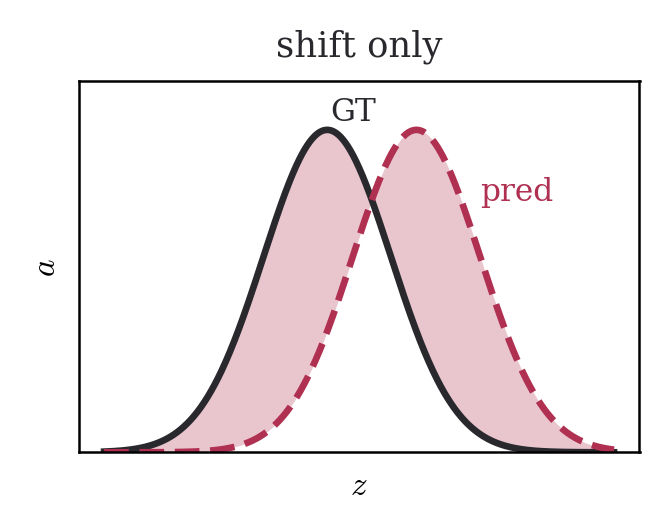
\includegraphics[width=\linewidth]{../figures/error_landscape/shift_only_profile.png}
        \end{column}
        \begin{column}{0.48\linewidth}
          \centering
          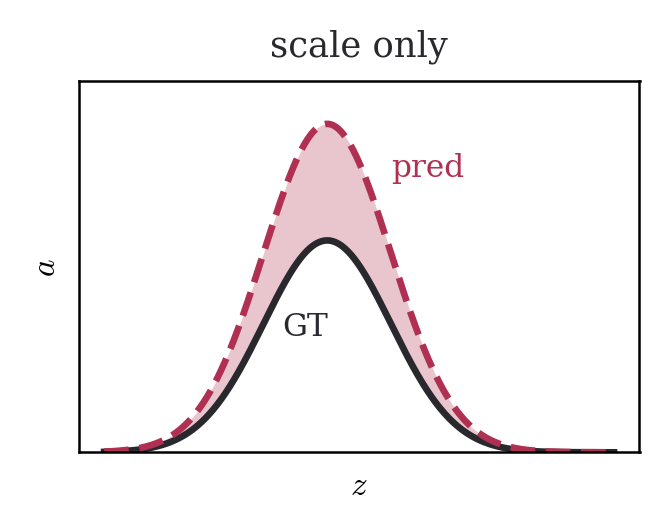
\includegraphics[width=\linewidth]{../figures/error_landscape/scale_only_profile.png}
        \end{column}
      \end{columns}
    \end{column}
  \end{columns}
\end{frame}

% ---------------------------------------------------------------- 25e-b Math: the joint error landscape
\begin{frame}{Shift and scale together --- the joint error}
  \setlength{\abovedisplayskip}{3pt}
  \setlength{\belowdisplayskip}{3pt}
  \begin{columns}[c]
    \begin{column}{0.52\textwidth}
      \small
      \begin{itemize}
        \item \textbf{Both mistakes at once} --- the prediction scaled by
              $1{+}\varepsilon$ \emph{and} misplaced by $\delta$:
      \end{itemize}
      \[
      \begin{aligned}
        & \lVert (1{+}\varepsilon)\,\mathcal N_{\mu+\delta}-\mathcal N_{\mu}\rVert^2\\[2pt]
        \Longrightarrow\;\; & \;=\; (1{+}\varepsilon)^2E + E - 2\,(1{+}\varepsilon)\,\langle\mathcal N_{\mu+\delta},\,\mathcal N_{\mu}\rangle\\[2pt]
        \Longrightarrow\;\; & \hleq{\;=\; E\,\big[(1{+}\varepsilon)^2 + 1 - 2\,(1{+}\varepsilon)\,e^{-\delta^2/4\sigma^2}\big]}\\[2pt]
        \Longrightarrow\;\; & \varepsilon{=}0:\ 2E\big(1-e^{-\delta^2/4\sigma^2}\big), \qquad \delta{=}0:\ \varepsilon^2E
      \end{aligned}
      \]

      \smallskip
      \begin{itemize}
        \item \textbf{Take the partial derivatives:}
      \end{itemize}
      \[
      \begin{aligned}
        & \tfrac{\partial}{\partial\delta}\,\lVert(1{+}\varepsilon)\,\mathcal N_{\mu+\delta}-\mathcal N_{\mu}\rVert^2 \;=\; (1{+}\varepsilon)\,\tfrac{E\,\delta}{\sigma^2}\,e^{-\delta^2/4\sigma^2}\\[2pt]
        & \tfrac{\partial}{\partial\varepsilon}\,\lVert(1{+}\varepsilon)\,\mathcal N_{\mu+\delta}-\mathcal N_{\mu}\rVert^2 \;=\; 2E\,\big(1{+}\varepsilon-e^{-\delta^2/4\sigma^2}\big)\\[2pt]
        \Longrightarrow\;\; & \tfrac{\partial}{\partial\delta} = 0 \ \text{ at } \ \delta \;=\; 0 \ \text{ (any } \varepsilon)\\[2pt]
        \Longrightarrow\;\; & \hleq{\tfrac{\partial}{\partial\varepsilon} = 0 \ \text{ at } \ 1{+}\varepsilon \;=\; e^{-\delta^2/4\sigma^2} \;<\; 1}
      \end{aligned}
      \]
    \end{column}
    \begin{column}{0.46\textwidth}
      \centering
      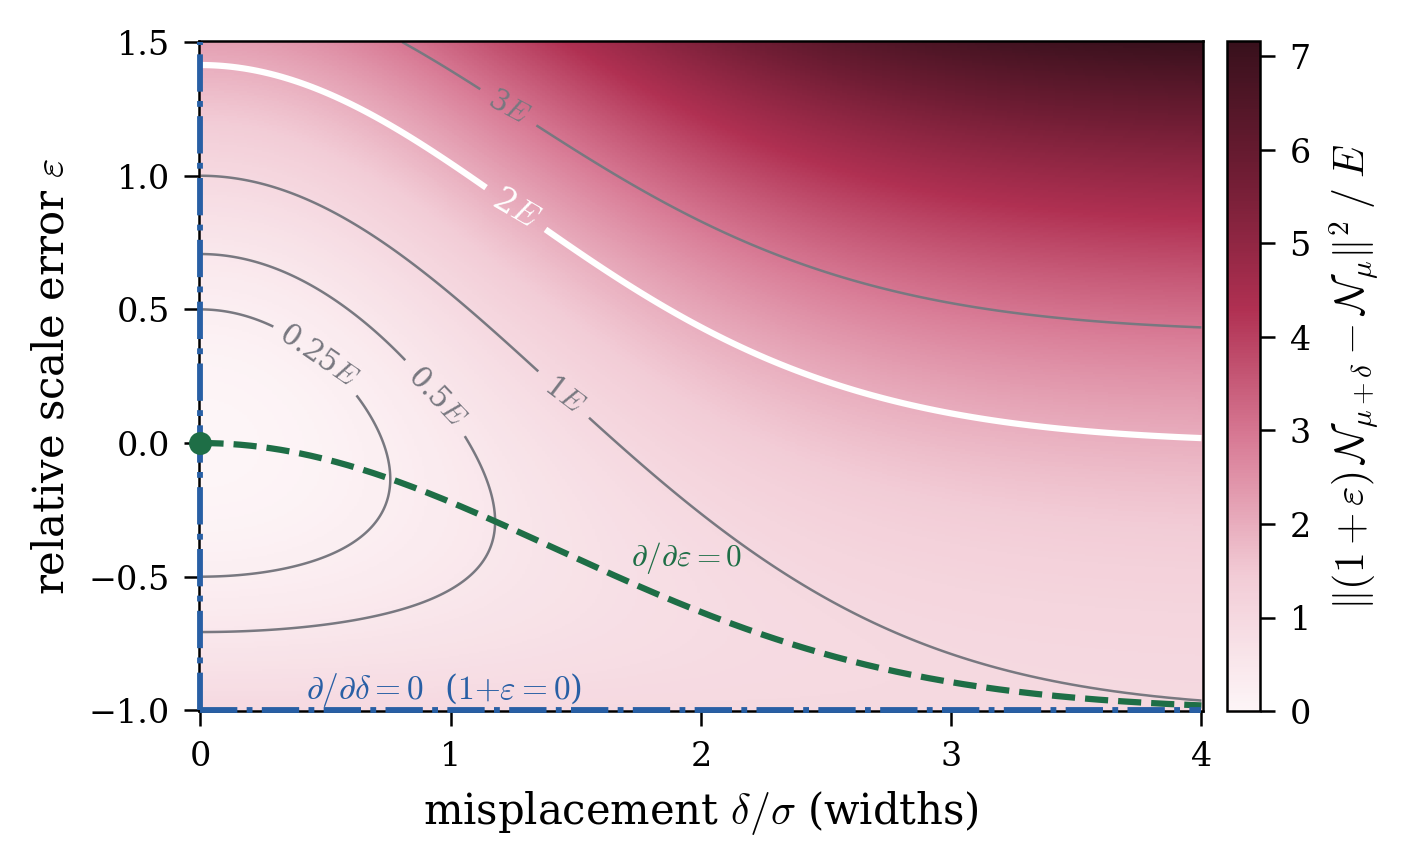
\includegraphics[width=\linewidth]{../figures/error_landscape/joint_error_heatmap.png}\\[2pt]
      {\scriptsize\color{soft} the joint landscape: the critical curves meet
      only at the truth --- the surface's one minimum.\par}
    \end{column}
  \end{columns}
\end{frame}

% ---------------------------------------------------------------- 25e-c Math: convergence and the training pull
\begin{frame}{The bowl and the training pull}
  \setlength{\abovedisplayskip}{3pt}
  \setlength{\belowdisplayskip}{3pt}
  \small
  Zoom into small $\delta$, $\varepsilon$ --- the regime of a converging
  network:
  \begin{columns}[T]
    \begin{column}{0.5\textwidth}
      \centering
      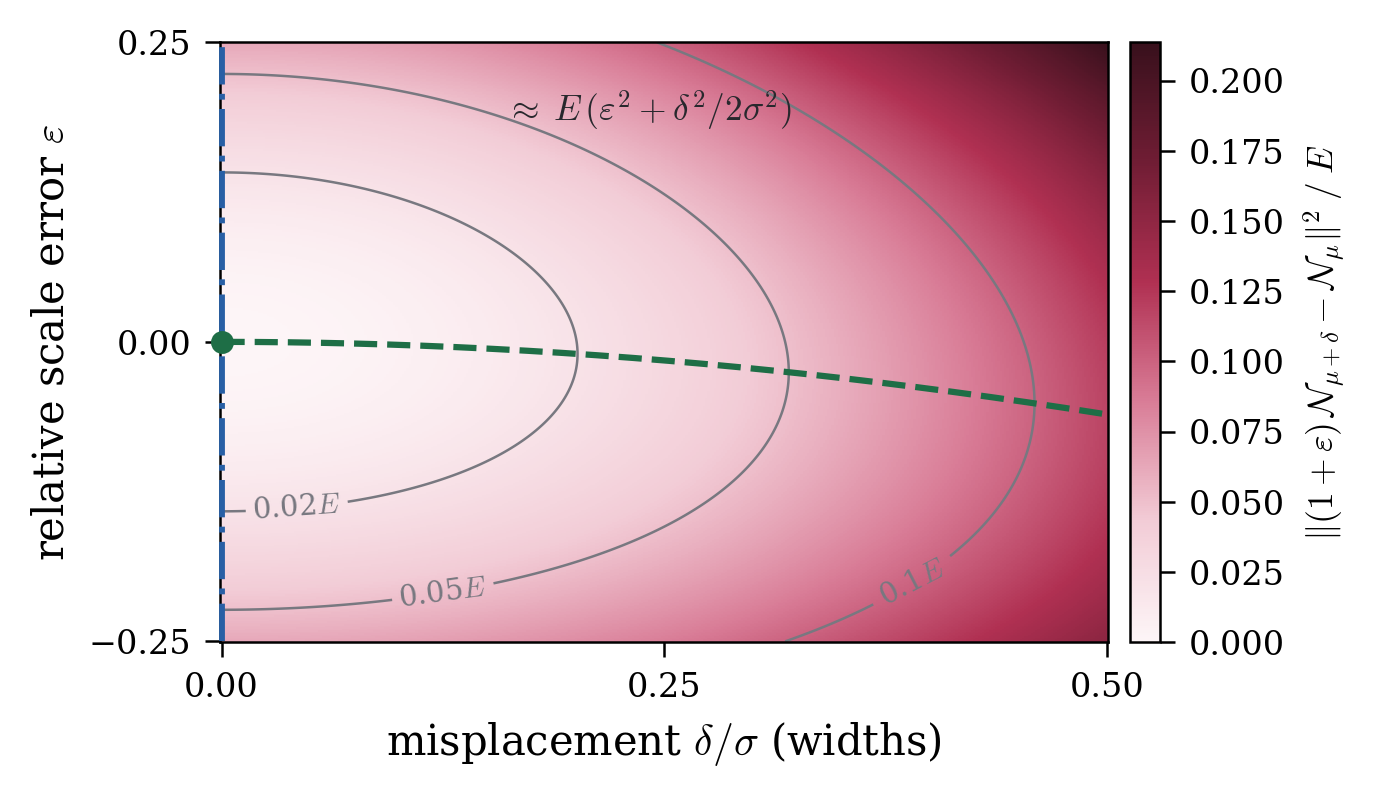
\includegraphics[width=\linewidth]{../figures/error_landscape/joint_error_convergence.png}
    \end{column}
    \begin{column}{0.5\textwidth}
      \centering
      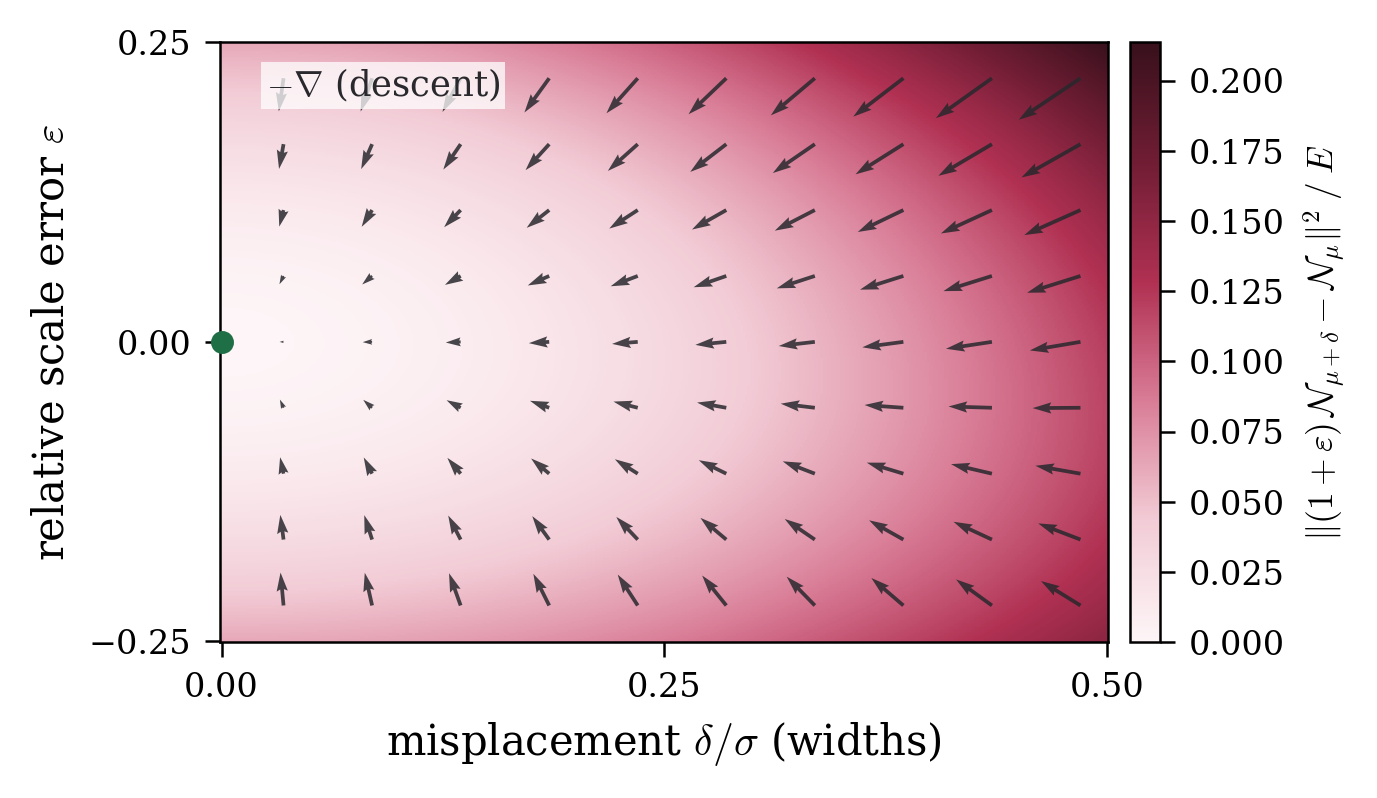
\includegraphics[width=\linewidth]{../figures/error_landscape/joint_error_gradient.png}
    \end{column}
  \end{columns}
  \smallskip
  {\scriptsize\color{soft} left: the quadratic bowl --- elliptic contours,
  valley tangent to $\varepsilon{=}0$, no plateau. right: the $-\nabla$
  descent field --- onto the valley at curvature $2E$, along it at $E$; its
  dim drift feeds the recall paradox (two frames ahead).\par}
\end{frame}

% ---------------------------------------------------------------- 25e-d Math: the K-scatterer sum decouples
\begin{frame}{The full profile --- separated scatterers decouple}
  \setlength{\abovedisplayskip}{3pt}
  \setlength{\belowdisplayskip}{3pt}
  \begin{columns}[c]
    \begin{column}{0.49\textwidth}
      \small
      \begin{itemize}
        \item \textbf{Write the error as residuals.} Truth and
              prediction are sums of $K$ components; Hungarian pairing matches
              them one to one, so pair $k$ owns its shift $\delta_k$ and scale
              error $\varepsilon_k$:
      \end{itemize}
      \[
      \begin{aligned}
        & p = \textstyle\sum_{k} \mathcal N_{\mu_k}, \qquad \hat p = \textstyle\sum_{k} (1{+}\varepsilon_k)\,\mathcal N_{\mu_k+\delta_k}\\[3pt]
        \Longrightarrow\;\; & \hat p - p \;=\; \textstyle\sum_{k} r_k, \qquad r_k = (1{+}\varepsilon_k)\,\mathcal N_{\mu_k+\delta_k} - \mathcal N_{\mu_k}
      \end{aligned}
      \]
      {\scriptsize\color{soft} $\mathcal N_{\mu_k}$: the $k$-th component
      $a_k\,\mathcal N(z;\mu_k,\sigma_k)$, energy
      $E_k=\lVert\mathcal N_{\mu_k}\rVert^2=a_k^2/(2\sqrt{\pi}\,\sigma_k)$;
      $r_k$: its residual.\par}
      \vspace{16pt}
      \begin{itemize}
        \item \textbf{Square the sum} --- bilinearity, no approximation:
      \end{itemize}
      \[
      \begin{aligned}
        & \lVert \hat p - p \rVert^2 \;=\; \textstyle\sum_{k} \lVert r_k \rVert^2 \;+\; 2\textstyle\sum_{j<k} \langle r_j, r_k \rangle\\[3pt]
        & \lVert r_k \rVert^2 \;=\; E_k\big[(1{+}\varepsilon_k)^2 + 1 - 2\,(1{+}\varepsilon_k)\,e^{-\delta_k^2/4\sigma_k^2}\big]
      \end{aligned}
      \]
    \end{column}
    \begin{column}{0.49\textwidth}
      \small
      \begin{itemize}
        \item \textbf{Assume the scatterers are separated.} Any two
              Gaussian components overlap in closed form --- exponentially
              small in the distance between their centres $m$, $m'$:
      \end{itemize}
      \[
      \begin{aligned}
        & \big\langle a_j\,\mathcal N(z;m,\sigma_j),\, a_k\,\mathcal N(z;m',\sigma_k) \big\rangle \\[2pt]
        & \;\propto\; e^{-(m-m')^2/2(\sigma_j^2+\sigma_k^2)}
      \end{aligned}
      \]
      \smallskip
      $\langle r_j, r_k\rangle$ is four such overlaps, centred near $\mu_j$
      and $\mu_k$. Assume the separation is big enough --- a few joint
      widths --- and all four cancel:
      \[
      \begin{aligned}
        & |\mu_j - \mu_k| \;\ge\; 3\,\sqrt{\sigma_j^2+\sigma_k^2}\\[2pt]
        \Longrightarrow\;\; & e^{-(\mu_j-\mu_k)^2/2(\sigma_j^2+\sigma_k^2)} \;\le\; e^{-9/2} \;\approx\; 0.01\\[2pt]
        \Longrightarrow\;\; & \hleq{\langle r_j, r_k\rangle \approx 0 \;\;\Longrightarrow\;\; \lVert\hat p - p\rVert^2 \;\approx\; \textstyle\sum_k \lVert r_k \rVert^2}
      \end{aligned}
      \]
    \end{column}
  \end{columns}
\end{frame}

% ---------------------------------------------------------------- 25f Math: the recall paradox
\begin{frame}{The recall paradox --- MSE turns doubt into dimming}
  \setlength{\abovedisplayskip}{4pt}
  \setlength{\belowdisplayskip}{4pt}
  \begin{columns}[c]
    \begin{column}{0.49\textwidth}
      \small
      \begin{itemize}
        \item \textbf{Squared error is minimised by the conditional mean} ---
              the value the loss pulls every output toward:
      \end{itemize}
      \[
        \hat a_2(x) \;=\; \mathrm E\,[\,a_2 \mid x\,]
      \]
      {\scriptsize\color{soft} $x$: the input patch; $a_2$: the second
      amplitude label --- defined as $0$ on pixels with a single scatterer
      ($K{=}1$).\par}
      \smallskip
      \begin{itemize}
        \item \textbf{Split the mean over the two cases.} The label is zero in
              one case and bright in the other; the zero case drops:
      \end{itemize}
      \[
      \begin{aligned}
        \hat a_2 \;&=\; \Pr(K{=}2\,|\,x)\,\mathrm E[a_2\,|\,K{=}2,x]\\[2pt]
        &\quad \;+\; \Pr(K{=}1\,|\,x)\,\mathrm E[a_2\,|\,K{=}1,x]\\[4pt]
        &\hleq{=\; \Pr(K{=}2\,|\,x) \cdot \mathrm E[a_2\,|\,K{=}2,x]}
      \end{aligned}
      \]
      \smallskip
      \begin{itemize}
        \item \textbf{Bayes' rule}, with $\pi=\Pr(K{=}2)$, and total
              probability over the two cases:
      \end{itemize}
      \[
      \begin{aligned}
        \Pr(K{=}2\,|\,x) \;&=\; \tfrac{p(x\,|\,K{=}2)\,\pi}{p(x\,|\,K{=}2)\,\pi \,+\, p(x\,|\,K{=}1)\,(1{-}\pi)}\\[3pt]
        &=\; \tfrac{\pi\,\Lambda}{1-\pi+\pi\,\Lambda}, \qquad
        \Lambda(x) \;=\; \tfrac{p(x\,|\,K{=}2)}{p(x\,|\,K{=}1)}
      \end{aligned}
      \]
\end{column}
    \begin{column}{0.49\textwidth}
      \small
      \begin{itemize}
        \item \textbf{$|A|$ runs:}
      \end{itemize}
      \[
      \begin{aligned}
        & \Lambda(x)\approx1\ \text{on every pixel} \ \Rightarrow\ \Pr(K{=}2\,|\,x)\approx\pi\\[1pt]
        & \Rightarrow\ \hat a_2 \ \text{pulled to} \ \pi\cdot\mathrm E[a_2\,|\,K{=}2,x]\\[2pt]
        & \Rightarrow\ \mathrm E[a_2\,|\,K{=}2,x] \;=\; f_\theta(P(x))\\[2pt]
        & \hleq{\hat a_2 \;=\; \pi\cdot f_\theta(P(x)) \ \text{--- dimmed}}\\[2pt]
        & \Rightarrow\ f_\theta(P(x)) \to 0, \ \text{class imbalance}
      \end{aligned}
      \]
      \smallskip
      \begin{itemize}
        \item \textbf{$\varphi$-only:} every pixel lands at an extreme:
      \end{itemize}
      \[
      \begin{aligned}
        & \Lambda(x)\gg1\ \text{on true pairs} \ \Rightarrow\ \Pr(K{=}2\,|\,x)\to1\\[1pt]
        & \hleq{\Rightarrow\ \hat a_2\to\mathrm E[a_2\,|\,K{=}2,x] \ \text{--- undimmed}}\\[2pt]
        & \hat a_2 = \mathrm E[a_2|K{=}2,x] = \mathrm E[a_2|K{=}2] = \bar a_2^{\mathrm{active}}\\[6pt]
        & \Lambda(x)\ll1\ \text{on singles} \ \Rightarrow\ \Pr(K{=}2\,|\,x)\to0\\[1pt]
        & \Rightarrow\ \hat a_2\to0 \ \text{--- the slot closes}
      \end{aligned}
      \]
    \end{column}
  \end{columns}
\end{frame}


\act{V \ \ Benchmark}{run-health tooling \; $\cdot$ \; every backbone $\times$ every objective \; $\cdot$ \; one winner \; $\cdot$ \; dual trunks}

% ---------------------------------------------------------------- 26 Tooling
\begin{frame}{Run-health tooling: no GPU-hour starts unhealthy}
  \centering
  \begin{tikzpicture}[node distance=6mm]
    \node[box, text width=26mm] (size) {\textbf{capacity match}\\{\tiny every backbone width-scaled\\to $\approx$30\,M parameters}};
    \node[box, text width=26mm, right=of size] (gate) {\textbf{overfit gate}\\{\tiny model must overfit a tiny\\subset or the run aborts}};
    \node[box, text width=26mm, right=of gate] (batch) {\textbf{max-batch finder}\\{\tiny largest batch that fits VRAM,\\probed with the real loss}};
    \node[box, text width=26mm, right=of batch] (feed) {\textbf{DataLoader tuner}\\{\tiny workers / prefetch / pinning\\to keep the GPU fed}};
    \draw[flow] (size) -- (gate);
    \draw[flow] (gate) -- (batch);
    \draw[flow] (batch) -- (feed);
  \end{tikzpicture}
  \\[8pt]
  {\footnotesize
  \setlength{\tabcolsep}{6pt}
  \renewcommand{\arraystretch}{1.2}
  \begin{tabular}{@{}r l@{}}
    \textbf{7 backbones}   & unet, unet\_skip, resunet, attention\_unet, deeplabv3plus, segformer, nafnet\\
    \textbf{5 objectives}  & curve space: MSE, L1, Charbonnier \;$\cdot$\; parameter space: MSE, L1\\
    \textbf{1 head, fixed} & gated set prediction $\cdot$ Hungarian matching --- the Act III verdict, baked into every cell\\
    \textbf{5 seeds}       & every cell trained five times --- $35$ configurations $\times$ $5$ seeds $=$ $175$ runs, reported mean $\pm$ seed std\\
  \end{tabular}}
  \\[8pt]
  \small
  \begin{itemize}
    \item Capacity is matched, the recipe is identical in every cell (set-pred $\cdot$
          Hungarian $\cdot$ presence lever A $\cdot$ hv flips $\cdot$ $K{=}2$; reference
          cell \textbf{UNet + param-MSE}) --- differences are architectural, not capacity.
    \item A model that cannot memorise a handful of patches has a plumbing, loss or
          architecture bug --- caught in minutes, not after hours. Surrogate-loss memory
          probes understate the footprint $\approx$$10\times$, so the batch is probed
          with the genuine training step and the LR auto-scales with it.
    \item Payoff: the benchmark grid runs unattended --- a dead cell means a real model
          failure, not an infrastructure one.
  \end{itemize}
\end{frame}

% ---------------------------------------------------------------- 29g Completed board
\begin{frame}{The board at five seeds --- the L1 family owns the top nine}
    \centering
  \scriptsize
  \renewcommand{\arraystretch}{0.95}
  \setlength{\tabcolsep}{4pt}
  \renewcommand{\seedtag}{bbA}
  \begin{tabular}{@{}c l l c c c c c@{}}
    \toprule
    \# & model & loss & curve $R^2$ $\uparrow$ & cosine $\uparrow$ & peak err $\downarrow$ & recall $\uparrow$ & score \\
    \midrule
    1 & unet-skip & L1-curve & \seedpm{\textbf{0.756}}{.012} & \seedpm{0.924}{.007} & \seedpm{1.29}{.05} & \seedpm{0.886}{.006} & \hlval{good}{\textbf{0.983}} \\
    2 & unet-skip & Charbonnier & \seedpm{0.751}{.012} & \seedpm{0.928}{.004} & \seedpm{\textbf{1.25}}{.03} & \seedpm{0.886}{.004} & 0.977 \\
    3 & unet-skip & param-L1 & \seedpm{0.741}{.016} & \seedpm{\textbf{0.931}}{.001} & \seedpm{1.38}{.03} & \seedpm{0.893}{.004} & 0.963 \\
    \addlinespace[2pt]
    4 & resunet & param-L1 & \seedpm{0.734}{.013} & \seedpm{0.927}{.007} & \seedpm{1.32}{.07} & \seedpm{0.894}{.003} & 0.946 \\
    5 & deeplab & param-L1 & \seedpm{0.731}{.006} & \seedpm{0.923}{.004} & \seedpm{1.35}{.05} & \seedpm{0.888}{.002} & 0.937 \\
    6 & deeplab & L1-curve & \seedpm{0.731}{.012} & \seedpm{0.921}{.013} & \seedpm{1.33}{.07} & \seedpm{0.873}{.022} & 0.935 \\
    7 & resunet & L1-curve & \seedpm{0.737}{.019} & \seedpm{0.916}{.007} & \seedpm{1.34}{.06} & \seedpm{0.881}{.005} & 0.930 \\
    8 & resunet & Charbonnier & \seedpm{0.731}{.016} & \seedpm{0.921}{.014} & \seedpm{1.31}{.08} & \seedpm{0.881}{.006} & 0.929 \\
    9 & deeplab & Charbonnier & \seedpm{0.735}{.008} & \seedpm{0.913}{.015} & \seedpm{1.62}{.45} & \seedpm{0.868}{.037} & 0.912 \\
    10 & nafnet & Charbonnier & \seedpm{0.702}{.009} & \seedpm{0.906}{.007} & \seedpm{1.48}{.05} & \seedpm{0.875}{.008} & 0.829 \\
    11 & segformer & Charbonnier & \seedpm{0.688}{.022} & \seedpm{0.910}{.016} & \seedpm{1.51}{.20} & \seedpm{0.866}{.019} & 0.829 \\
    12 & nafnet & L1-curve & \seedpm{0.698}{.007} & \seedpm{0.908}{.010} & \seedpm{1.43}{.08} & \seedpm{0.879}{.005} & 0.828 \\
    \multicolumn{8}{c}{{\color{soft}$\vdots$}} \\
    16 & deeplab & MSE-curve & \seedpm{0.732}{.010} & \seedpm{0.872}{.019} & \seedpm{1.62}{.08} & \seedpm{0.869}{.004} & 0.785 \\
    \addlinespace[2pt]
    20 & unet & L1-curve & \seedpm{0.660}{.015} & \seedpm{0.897}{.026} & \seedpm{1.51}{.28} & \seedpm{0.870}{.029} & 0.760 \\
    \addlinespace[2pt]
    21 & unet-skip & param-MSE & \seedpm{0.647}{.047} & \seedpm{0.879}{.017} & \seedpm{1.59}{.13} & \seedpm{0.881}{.022} & \hlval{accent}{0.692} \\
    \bottomrule
  \end{tabular}
  \par\vspace{2pt}
  \parbox{0.82\textwidth}{\tiny\color{soft} runs: model $\cdot$ set-pred $\cdot$ Hungarian $\cdot$
   $K{=}2$ $\cdot$ hv flips $\cdot$ presence A $\cdot$ loss $\cdot$ patch
   $64{\times}32$, five seeds; held-out band. Cells: mean $\pm$ seed std;
   \textbf{bold} $=$ best mean in column (rows shown), marked only where best and worst differ by more than $5\%$. score $=$ equal-weight mean
   of the five metric groups (curve error, variance, SSIM, cosine, peak), min--max
   scaled over the 35 arms; \# $=$ rank; ranks 13--15, 17--19, 22--35 on the next
   frame only. cosine $=$ per-pixel profile cosine mean; peak err in elevation
   units; recall $=$ matched. \textcolor{good}{green} $=$ the winner's score; \textcolor{accent}{red} $=$ the param-MSE reference cell, 21st of 35.\par}
    

\end{frame}

% ---------------------------------------------------------------- 29gB Board by scatterer count
\begin{frame}{The board by scatterer count --- curve-MSE drops the single scatterer}
    \centering
  \scriptsize
  \renewcommand{\arraystretch}{1.00}
  \setlength{\tabcolsep}{2.5pt}
  \renewcommand{\seedtag}{bbB}
  \begin{tabular}{@{}l c c c c c !{\hspace{3pt}} c@{}}
    \toprule
    & \multicolumn{5}{c}{UNet-skip --- winner backbone} & \multicolumn{1}{c@{}}{UNet} \\
    \cmidrule(lr){2-6}\cmidrule(l){7-7}
    metric & L1 & Charb. & param-L1 & MSE & param-MSE & param-MSE \\
    \midrule
    matched precision $\uparrow$ & \seedpm{0.893}{.005} & \seedpm{0.896}{.006} & \seedpm{\textbf{0.900}}{.001} & \seedpm{0.858}{.012} & \seedpm{0.816}{.041} & \seedpm{0.820}{.006} \\
    \quad $k{=}1$ & \seedpm{0.916}{.006} & \seedpm{0.922}{.008} & \seedpm{\textbf{0.948}}{.002} & \seedpm{0.883}{.016} & \seedpm{0.830}{.059} & \seedpm{0.843}{.008} \\
    \quad $k{=}2$ & \seedpm{\textbf{0.850}}{.005} & \seedpm{\textbf{0.850}}{.004} & \seedpm{0.821}{.002} & \seedpm{0.821}{.006} & \seedpm{0.792}{.011} & \seedpm{0.779}{.006} \\
    \addlinespace
    matched recall $\uparrow$ & \seedpm{0.886}{.006} & \seedpm{0.886}{.004} & \seedpm{0.893}{.004} & \seedpm{\hlval{accent}{0.766}}{.072} & \seedpm{0.881}{.022} & \seedpm{\textbf{0.894}}{.002} \\
    \quad $k{=}1$ & \seedpm{0.997}{.002} & \seedpm{\textbf{0.998}}{.001} & \seedpm{0.997}{.001} & \seedpm{\hlval{accent}{0.808}}{.122} & \seedpm{0.981}{.030} & \seedpm{0.997}{.001} \\
    \quad $k{=}2$ & \seedpm{0.728}{.013} & \seedpm{0.727}{.008} & \seedpm{0.745}{.008} & \seedpm{0.707}{.013} & \seedpm{0.739}{.014} & \seedpm{\textbf{0.748}}{.003} \\
    \addlinespace
    count acc\,$\mid$\,pred $k{=}1$\,$\uparrow$ & \seedpm{0.910}{.006} & \seedpm{0.906}{.006} & \seedpm{0.950}{.003} & \seedpm{0.922}{.014} & \seedpm{\textbf{0.973}}{.008} & \seedpm{\textbf{0.973}}{.004} \\
    count acc\,$\mid$\,pred $k{=}2$\,$\uparrow$ & \seedpm{0.740}{.011} & \seedpm{0.753}{.015} & \seedpm{\hlval{good}{\textbf{0.847}}}{.005} & \seedpm{0.723}{.010} & \seedpm{0.621}{.083} & \seedpm{0.640}{.013} \\
    count exact $\uparrow$ & \seedpm{0.861}{.002} & \seedpm{0.865}{.002} & \seedpm{\textbf{0.917}}{.004} & \seedpm{0.723}{.088} & \seedpm{0.812}{.082} & \seedpm{0.845}{.008} \\
    \addlinespace
    matched $\mu$ MAE $\downarrow$ & \seedpm{1.49}{.04} & \seedpm{\textbf{1.48}}{.03} & \seedpm{1.72}{.04} & \seedpm{2.01}{.16} & \seedpm{1.94}{.09} & \seedpm{2.19}{.17} \\
    \quad $k{=}1$ & \seedpm{0.39}{.04} & \seedpm{0.37}{.02} & \seedpm{\textbf{0.34}}{.01} & \seedpm{0.68}{.11} & \seedpm{0.50}{.05} & \seedpm{0.71}{.23} \\
    \quad $k{=}2$ & \seedpm{\textbf{3.32}}{.06} & \seedpm{3.33}{.03} & \seedpm{3.87}{.07} & \seedpm{3.76}{.08} & \seedpm{4.11}{.15} & \seedpm{4.38}{.13} \\
    \addlinespace
    matched $\sigma$ MAE $\downarrow$ & \seedpm{0.77}{.04} & \seedpm{0.78}{.01} & \seedpm{0.73}{.01} & \seedpm{1.17}{.07} & \seedpm{\textbf{0.72}}{.02} & \seedpm{0.81}{.01} \\
    \quad $k{=}1$ & \seedpm{0.22}{.01} & \seedpm{0.23}{.02} & \seedpm{\textbf{0.20}}{.00} & \seedpm{0.39}{.02} & \seedpm{0.21}{.02} & \seedpm{0.24}{.01} \\
    \quad $k{=}2$ & \seedpm{1.67}{.08} & \seedpm{1.70}{.05} & \seedpm{1.57}{.03} & \seedpm{2.21}{.04} & \seedpm{\textbf{1.48}}{.03} & \seedpm{1.66}{.03} \\
    \addlinespace
    matched $a$ MAE $\downarrow$ & \seedpm{0.241}{.011} & \seedpm{0.242}{.008} & \seedpm{\hlval{good}{\textbf{0.175}}}{.002} & \seedpm{0.387}{.030} & \seedpm{0.223}{.010} & \seedpm{0.307}{.011} \\
    \quad $k{=}1$ & \seedpm{0.090}{.008} & \seedpm{0.090}{.011} & \seedpm{\textbf{0.055}}{.001} & \seedpm{0.176}{.030} & \seedpm{0.089}{.012} & \seedpm{0.125}{.011} \\
    \quad $k{=}2$ & \seedpm{0.491}{.024} & \seedpm{0.494}{.013} & \seedpm{\textbf{0.363}}{.007} & \seedpm{0.669}{.020} & \seedpm{0.424}{.011} & \seedpm{0.576}{.017} \\
    \bottomrule
  \end{tabular}
  \par\vspace{3pt}
  \parbox{0.82\textwidth}{\tiny\color{soft} \textbf{runs}: UNet-skip / UNet $\cdot$ set-pred $\cdot$
   Hungarian $\cdot$ $K{=}2$ $\cdot$ hv flips $\cdot$ presence A $\cdot$ patch
   $64{\times}32$ (backbone $\cdot$ objective = column); held-out validation band,
   cells mean $\pm$ seed std over five seeded replicas; $k$ $=$ true scatterer
   count of the pixel. \textbf{bold} $=$ best in row, marked only where best and worst differ by more than $5\%$. Precision rewards
   under-prediction --- rank on recall. count acc $\mid$ pred $k$: share of pixels
   claiming exactly $k$ scatterers whose true count is $k$. $\mu$, $\sigma$ in
   elevation units; $a$ in linear amplitude. \textcolor{good}{green} $=$ param-L1's count and amplitude calibration; \textcolor{accent}{red} $=$ curve-MSE dropping the single scatterer.\par}
    

\end{frame}

% ---------------------------------------------------------------- 29gC Board predicted stats vs GT
\begin{frame}{The board, predicted statistics vs the GT --- the gate sets activity, param-L1 calibrates amplitude}
    \centering
  \scriptsize
  \renewcommand{\arraystretch}{0.90}
  \setlength{\tabcolsep}{0.35pt}
  \renewcommand{\seedtag}{bbC}
  \begin{tabular}{@{}l !{\color{white}\vrule width 1.2pt} c !{\color{white}\vrule width 1.2pt} c c c c c !{\hspace{1pt}} c@{}}
    \toprule
    & & \multicolumn{5}{c}{UNet-skip --- winner backbone} & \multicolumn{1}{c@{}}{UNet} \\
    \cmidrule(lr){3-7}\cmidrule(l){8-8}
    prediction mean & \textcolor{good}{GT} & L1 & Charb. & param-L1 & MSE & param-MSE & param-MSE \\
    \midrule
    \multicolumn{8}{@{}l}{\textcolor{soft}{\emph{slot 0 --- strongest scatterer; GT-active on every pixel}}} \\
    \quad active frac & 1.00 & \seedpm{0.97}{.01} & \seedpm{0.97}{.00} & \seedpm{0.98}{.00} & \seedpm{\hlval{accent}{0.82}}{.09} & \seedpm{0.97}{.02} & \seedpm{\textbf{0.99}}{.00} \\
    \addlinespace[2pt]
    \quad $a$ --- active & 0.77 & \seedpm{0.66}{.01} & \seedpm{0.66}{.00} & \seedpm{\hlval{good}{\textbf{0.74}}}{.00} & \seedpm{0.65}{.06} & \seedpm{0.72}{.02} & \seedpm{0.59}{.02} \\
    \quad $\mu$ --- active & $-$4.89 & \seedpm{$-$4.50}{.12} & \seedpm{\textbf{$-$4.56}}{.11} & \seedpm{$-$4.52}{.04} & \seedpm{$-$4.02}{.24} & \seedpm{$-$4.19}{.09} & \seedpm{$-$4.08}{.21} \\
    \quad $\sigma$ --- active & 1.76 & \seedpm{1.39}{.05} & \seedpm{1.37}{.06} & \seedpm{1.38}{.01} & \seedpm{\textbf{1.59}}{.13} & \seedpm{1.41}{.06} & \seedpm{1.38}{.05} \\
    \addlinespace[1.5pt]
    \multicolumn{8}{@{}l}{\textcolor{soft}{\emph{slot 1 --- second scatterer; GT-active on 26\% of pixels}}} \\
    \quad active frac & 0.260 & \seedpm{0.280}{.010} & \seedpm{\textbf{0.274}}{.011} & \seedpm{\textbf{0.274}}{.003} & \seedpm{0.301}{.007} & \seedpm{0.392}{.059} & \seedpm{0.384}{.009} \\
    \addlinespace[2pt]
    \quad $a$ --- active & 1.43 & \seedpm{1.25}{.07} & \seedpm{1.24}{.05} & \seedpm{\hlval{good}{\textbf{1.42}}}{.02} & \seedpm{1.05}{.05} & \seedpm{1.32}{.05} & \seedpm{0.95}{.02} \\
    \quad $a$ --- inact. & 0.00 & \seedpm{0.69}{.02} & \seedpm{0.71}{.07} & \seedpm{0.88}{.06} & \seedpm{0.54}{.04} & \seedpm{0.41}{.13} & \seedpm{\textbf{0.34}}{.05} \\
    \quad $\mu$ --- active & 11.34 & \seedpm{6.11}{.26} & \seedpm{5.99}{.19} & \seedpm{8.30}{.25} & \seedpm{6.41}{.16} & \seedpm{\textbf{8.77}}{.40} & \seedpm{8.18}{.39} \\
    \quad $\mu$ --- inact. & --- & \seedpm{0.35}{.73} & \seedpm{0.09}{.26} & \seedpm{0.83}{.30} & \seedpm{1.35}{.40} & \seedpm{$-$0.51}{1.26} & \seedpm{$-$0.17}{.62} \\
    \quad $\sigma$ --- active & 3.53 & \seedpm{3.98}{.15} & \seedpm{3.93}{.20} & \seedpm{\textbf{3.22}}{.03} & \seedpm{5.57}{.16} & \seedpm{3.10}{.13} & \seedpm{2.77}{.05} \\
    \quad $\sigma$ --- inact. & --- & \seedpm{1.75}{.10} & \seedpm{1.79}{.06} & \seedpm{1.81}{.04} & \seedpm{3.42}{.14} & \seedpm{1.56}{.21} & \seedpm{1.64}{.08} \\
    \addlinespace[1.5pt]
    \multicolumn{8}{@{}l}{\textcolor{soft}{\emph{distribution width --- std over GT-active pixels}}} \\
    \quad $a$ --- slot 0 & 1.48 & \seedpm{1.23}{.07} & \seedpm{1.24}{.02} & \seedpm{\textbf{1.36}}{.02} & \seedpm{1.18}{.06} & \seedpm{1.35}{.08} & \seedpm{0.92}{.02} \\
    \quad $\mu$ --- slot 0 & 3.30 & \seedpm{1.98}{.07} & \seedpm{1.97}{.08} & \seedpm{2.56}{.06} & \seedpm{1.80}{.16} & \seedpm{\textbf{2.62}}{.11} & \seedpm{2.14}{.13} \\
    \quad $\sigma$ --- slot 0 & 2.84 & \seedpm{1.10}{.05} & \seedpm{1.05}{.08} & \seedpm{\textbf{1.23}}{.03} & \seedpm{1.08}{.05} & \seedpm{1.18}{.06} & \seedpm{1.03}{.05} \\
    \quad $a$ --- slot 1 & 1.45 & \seedpm{1.17}{.07} & \seedpm{1.16}{.04} & \seedpm{\textbf{1.29}}{.01} & \seedpm{1.01}{.04} & \seedpm{1.23}{.04} & \seedpm{0.83}{.03} \\
    \quad $\mu$ --- slot 1 & 16.24 & \seedpm{7.92}{.42} & \seedpm{7.93}{.39} & \seedpm{\textbf{9.98}}{.31} & \seedpm{7.15}{.35} & \seedpm{9.94}{.49} & \seedpm{8.88}{.48} \\
    \quad $\sigma$ --- slot 1 & 4.01 & \seedpm{2.08}{.14} & \seedpm{2.14}{.39} & \seedpm{1.77}{.04} & \seedpm{\textbf{2.68}}{.13} & \seedpm{1.56}{.06} & \seedpm{1.17}{.06} \\
    \bottomrule
  \end{tabular}
  \par\vspace{3pt}
  \parbox{0.82\textwidth}{\tiny\color{soft} \textbf{runs}: UNet-skip / UNet $\cdot$ set-pred $\cdot$
   Hungarian $\cdot$ $K{=}2$ $\cdot$ hv flips $\cdot$ presence A $\cdot$ patch
   $64{\times}32$ (backbone $\cdot$ objective = column); five seeded replicas per
   arm, cells mean $\pm$ seed std; means conditioned on the slot's GT activity
   mask. \textbf{bold} $=$ closest to the \textcolor{good}{GT} column, marked only where best and worst differ by more than $5\%$; inactive GT
   slots define no $\mu$/$\sigma$ reference (---). Width rows: std of the
   prediction over GT-active pixels vs the GT's own std. $\mu$, $\sigma$ in
   elevation units; $a$ in linear amplitude. \textcolor{good}{green} $=$ param-L1's amplitude calibration; \textcolor{accent}{red} $=$ curve-MSE's gate collapse.\par}
    

\end{frame}

% ---------------------------------------------------------------- 29g2 Full metrics board
\begin{frame}{Every headline metric, all 35 configurations}
  \centering
  \tiny
  \setlength{\tabcolsep}{2.4pt}
  \renewcommand{\arraystretch}{0.88}
  \begin{tabular}{@{}r l l c c c c c c c c c c c c c c c@{}}
    \toprule
    \# & model & loss & $R^2$ & PSNR & cosine & \shortstack{SSIM\\elev} & \shortstack{SSIM\\range} & \shortstack{SSIM\\azim} & F1 & recall & \shortstack{2-scatterer\\recall} & precision & $\mu$ MAE & $\sigma$ MAE & $a$ MAE & \shortstack{peak\\error} & score \\
    \midrule
    1 & unet-skip & L1-curve & \textbf{0.76} & 52.8 & 0.924 & 0.968 & 0.950 & 0.961 & 0.889 & 0.886 & 0.728 & 0.893 & 1.49 & 0.77 & 0.241 & 1.29 & \textbf{0.983} \\
    2 & unet-skip & Charbonnier & 0.75 & 52.7 & 0.928 & 0.967 & 0.950 & 0.961 & 0.891 & 0.886 & 0.727 & 0.896 & 1.48 & 0.78 & 0.242 & \textbf{1.25} & 0.977 \\
    3 & unet-skip & param-L1 & 0.74 & 52.5 & \textbf{0.931} & 0.967 & 0.951 & 0.961 & 0.897 & 0.893 & 0.745 & 0.900 & 1.72 & 0.73 & \textbf{0.175} & 1.38 & 0.963 \\
    4 & resunet & param-L1 & 0.73 & 52.4 & 0.927 & 0.966 & 0.950 & 0.960 & 0.898 & 0.894 & 0.746 & \textbf{0.902} & 1.75 & 0.76 & 0.178 & 1.32 & 0.946 \\
    5 & deeplab & param-L1 & 0.73 & 52.4 & 0.923 & 0.966 & 0.949 & 0.960 & 0.895 & 0.888 & 0.736 & \textbf{0.902} & 1.71 & \textbf{0.72} & 0.184 & 1.35 & 0.937 \\
    6 & deeplab & L1-curve & 0.73 & 52.4 & 0.921 & 0.967 & 0.949 & 0.960 & 0.876 & 0.873 & 0.721 & 0.879 & 1.52 & 0.74 & 0.241 & 1.33 & 0.935 \\
    7 & resunet & L1-curve & 0.74 & 52.5 & 0.916 & 0.967 & 0.949 & 0.960 & 0.890 & 0.881 & 0.715 & 0.900 & \textbf{1.46} & 0.77 & 0.238 & 1.34 & 0.930 \\
    8 & resunet & Charbonnier & 0.73 & 52.4 & 0.921 & 0.967 & 0.949 & 0.960 & 0.889 & 0.881 & 0.716 & 0.897 & 1.49 & 0.75 & 0.236 & 1.31 & 0.929 \\
    9 & deeplab & Charbonnier & 0.73 & 52.4 & 0.913 & 0.967 & 0.949 & 0.960 & 0.858 & 0.868 & 0.722 & 0.851 & 1.55 & 0.74 & 0.244 & 1.62 & 0.912 \\
    10 & nafnet & Charbonnier & 0.70 & 51.9 & 0.906 & 0.965 & 0.944 & 0.957 & 0.878 & 0.875 & 0.711 & 0.881 & 1.56 & 0.76 & 0.261 & 1.48 & 0.829 \\
    11 & segformer & Charbonnier & 0.69 & 51.7 & 0.910 & 0.965 & 0.945 & 0.957 & 0.873 & 0.866 & 0.704 & 0.881 & 1.54 & 0.76 & 0.265 & 1.51 & 0.829 \\
    12 & nafnet & L1-curve & 0.70 & 51.9 & 0.908 & 0.965 & 0.944 & 0.957 & 0.880 & 0.879 & 0.714 & 0.881 & 1.56 & 0.78 & 0.264 & 1.43 & 0.828 \\
    13 & segformer & param-L1 & 0.67 & 51.5 & 0.919 & 0.964 & 0.945 & 0.956 & 0.883 & 0.884 & 0.728 & 0.883 & 1.76 & 0.73 & 0.196 & 1.39 & 0.811 \\
    14 & segformer & L1-curve & 0.68 & 51.6 & 0.905 & 0.965 & 0.943 & 0.956 & 0.870 & 0.864 & 0.703 & 0.876 & 1.59 & 0.77 & 0.274 & 1.56 & 0.804 \\
    15 & nafnet & param-L1 & 0.67 & 51.5 & 0.917 & 0.963 & 0.945 & 0.956 & 0.885 & 0.883 & 0.724 & 0.888 & 1.77 & 0.75 & 0.198 & 1.43 & 0.797 \\
    \rowcolor{soft!18} 16 & deeplab & MSE-curve & 0.73 & 52.4 & 0.872 & 0.962 & 0.937 & 0.953 & 0.861 & 0.869 & 0.710 & 0.853 & 1.84 & 1.07 & 0.334 & 1.62 & 0.785 \\
    17 & att-unet & L1-curve & 0.67 & 51.4 & 0.899 & 0.965 & 0.945 & 0.957 & 0.863 & 0.885 & 0.725 & 0.843 & 1.77 & 0.83 & 0.312 & 1.44 & 0.772 \\
    18 & unet & Charbonnier & 0.66 & 51.4 & 0.901 & 0.965 & 0.945 & 0.957 & 0.866 & 0.880 & 0.713 & 0.854 & 1.69 & 0.79 & 0.324 & 1.45 & 0.772 \\
    19 & att-unet & Charbonnier & 0.67 & 51.4 & 0.890 & 0.965 & 0.944 & 0.957 & 0.862 & 0.884 & 0.723 & 0.842 & 1.79 & 0.81 & 0.307 & 1.47 & 0.764 \\
    20 & unet & L1-curve & 0.66 & 51.4 & 0.897 & 0.965 & 0.944 & 0.956 & 0.863 & 0.870 & 0.711 & 0.858 & 1.71 & 0.81 & 0.328 & 1.51 & 0.760 \\
    \rowcolor{soft!18} 21 & unet-skip & param-MSE & 0.65 & 51.2 & 0.879 & 0.963 & 0.940 & 0.954 & 0.847 & 0.881 & 0.739 & 0.816 & 1.94 & \textbf{0.72} & 0.223 & 1.59 & 0.692 \\
    \rowcolor{soft!18} 22 & resunet & param-MSE & 0.64 & 51.1 & 0.874 & 0.961 & 0.938 & 0.952 & 0.851 & 0.880 & 0.730 & 0.824 & 1.95 & 0.73 & 0.235 & 1.60 & 0.653 \\
    \rowcolor{soft!18} 23 & unet-skip & MSE-curve & 0.73 & 52.3 & 0.767 & 0.963 & 0.932 & 0.953 & 0.809 & 0.766 & 0.707 & 0.858 & 2.01 & 1.17 & 0.387 & 2.66 & 0.614 \\
    \rowcolor{soft!18} 24 & deeplab & param-MSE & 0.60 & 50.7 & 0.883 & 0.960 & 0.936 & 0.950 & 0.841 & 0.855 & 0.716 & 0.828 & 1.94 & 0.73 & 0.243 & 1.73 & 0.613 \\
    25 & unet & param-L1 & 0.61 & 50.8 & 0.855 & 0.963 & 0.940 & 0.953 & 0.893 & 0.886 & 0.725 & 0.900 & 2.01 & 0.80 & 0.251 & 1.56 & 0.610 \\
    26 & att-unet & param-L1 & 0.61 & 50.7 & 0.885 & 0.963 & 0.942 & 0.954 & 0.891 & 0.889 & 0.732 & 0.894 & 2.06 & 0.82 & 0.255 & 1.49 & 0.588 \\
    \rowcolor{soft!18} 27 & resunet & MSE-curve & 0.72 & 52.3 & 0.756 & 0.963 & 0.931 & 0.953 & 0.775 & 0.713 & 0.695 & 0.851 & 2.04 & 1.19 & 0.404 & 3.18 & 0.573 \\
    \rowcolor{soft!18} 28 & segformer & param-MSE & 0.57 & 50.4 & 0.868 & 0.959 & 0.934 & 0.947 & 0.832 & 0.871 & 0.702 & 0.796 & 2.03 & 0.75 & 0.243 & 1.68 & 0.532 \\
    \rowcolor{soft!18} 29 & unet & param-MSE & 0.58 & 50.4 & 0.829 & 0.960 & 0.934 & 0.949 & 0.856 & \textbf{0.894} & \textbf{0.748} & 0.820 & 2.19 & 0.81 & 0.307 & 1.67 & 0.484 \\
    \rowcolor{soft!18} 30 & att-unet & param-MSE & 0.58 & 50.4 & 0.853 & 0.960 & 0.934 & 0.949 & 0.853 & 0.892 & 0.742 & 0.817 & 2.16 & 0.81 & 0.311 & 1.66 & 0.477 \\
    \rowcolor{soft!18} 31 & nafnet & param-MSE & 0.58 & 50.4 & 0.877 & 0.958 & 0.932 & 0.946 & 0.837 & 0.871 & 0.709 & 0.807 & 2.09 & 0.79 & 0.260 & 1.69 & 0.437 \\
    \rowcolor{soft!18} 32 & segformer & MSE-curve & 0.67 & 51.5 & 0.712 & 0.956 & 0.922 & 0.945 & 0.741 & 0.676 & 0.676 & 0.823 & 2.17 & 1.45 & 0.448 & 3.89 & 0.346 \\
    \rowcolor{soft!18} 33 & unet & MSE-curve & 0.65 & 51.2 & 0.760 & 0.953 & 0.914 & 0.939 & 0.797 & 0.765 & 0.670 & 0.834 & 2.17 & 1.55 & 0.478 & 2.78 & 0.342 \\
    \rowcolor{soft!18} 34 & att-unet & MSE-curve & 0.63 & 51.0 & 0.759 & 0.951 & 0.911 & 0.936 & 0.818 & 0.802 & 0.680 & 0.837 & 2.21 & 1.66 & 0.466 & 2.47 & 0.307 \\
    \rowcolor{soft!18} 35 & nafnet & MSE-curve & 0.69 & 51.7 & 0.680 & 0.958 & 0.921 & 0.946 & 0.730 & 0.663 & 0.687 & 0.821 & 2.15 & 1.54 & 0.426 & 4.44 & 0.279 \\
    \bottomrule
  \end{tabular}
  \\[0pt]
  {\tiny\color{soft} Five-seed means vs GT (spreads on the previous frame and in the
   per-arm reports) --- PSNR in dB; cosine $=$ per-pixel profile cosine mean;
   F1 / recall / precision matched, 2-scatterer recall on GT $k{=}2$ pixels;
   $\mu$/$\sigma$ MAE and peak error in elevation units, $a$ MAE in linear amplitude;
   score $=$ five-group composite (row order). \textbf{Bold} $=$ best in column, marked only where best and worst differ by more than $5\%$; grey
   rows $=$ MSE-family objectives. runs: set-pred $\cdot$ Hungarian $\cdot$ $K{=}2$
   $\cdot$ hv flips $\cdot$ presence A $\cdot$ patch $64{\times}32$.\par}
\end{frame}

% ---------------------------------------------------------------- 29h Head vs matching decomposition
\begin{frame}{Where the gain comes from: the head, not the matching}
    \centering
  \scriptsize
  \renewcommand{\arraystretch}{1.02}
  \setlength{\tabcolsep}{5pt}
  \begin{tabular}{@{}l c c c c c c c@{}}
    \toprule
    loss & \shortstack{conv\\sorted} & \shortstack{conv\\Hungarian} & \shortstack{set-pred\\sorted} & \shortstack{set-pred\\Hungarian} & \shortstack{$\Delta$\\total} & \shortstack{$\Delta$\\head} & \shortstack{$\Delta$\\matching} \\
    \midrule
    \multicolumn{8}{@{}l}{\emph{ResUNet}} \\
    MSE-curve   & 0.608 & {\color{soft}--} & 0.926 & 0.926 & \textbf{+0.318} & \hlval{good}{+0.318} & {\color{soft}0.000} \\
    Huber-curve & 0.670 & {\color{soft}--} & 0.945 & 0.945 & \textbf{+0.275} & \hlval{good}{+0.275} & {\color{soft}0.000} \\
    Charbonnier & 0.914 & {\color{soft}--} & 0.991 & 0.991 & \textbf{+0.077} & \hlval{good}{+0.077} & {\color{soft}0.000} \\
    \addlinespace[2pt]
    param-MSE   & 0.937 & 0.924 & {\color{soft}--} & 0.939 & \textbf{+0.002} & +0.016 & {\color{soft}$-$0.013} \\
    param-Huber & 0.961 & 0.961 & {\color{soft}--} & 0.972 & \textbf{+0.011} & +0.011 & {\color{soft}0.000} \\
    param-L1    & 0.982 & 0.982 & 0.992 & 0.988 & \textbf{+0.006} & +0.006 & {\color{soft}$-$0.001} \\
    \addlinespace[1pt]
    \multicolumn{8}{@{}l}{\emph{Attention-UNet}} \\
    MSE-curve   & 0.556 & {\color{soft}--} & 0.807 & 0.671 & \textbf{+0.115} & \hlval{good}{+0.251} & {\color{soft}$-$0.136} \\
    Huber-curve & 0.624 & {\color{soft}--} & 0.929 & 0.922 & \textbf{+0.298} & \hlval{good}{+0.305} & {\color{soft}$-$0.007} \\
    Charbonnier & 0.790 & {\color{soft}--} & 0.960 & 0.962 & \textbf{+0.172} & \hlval{good}{+0.170} & {\color{soft}$+$0.003} \\
    \addlinespace[2pt]
    param-MSE   & 0.855 & 0.849 & {\color{soft}--} & 0.892 & \textbf{+0.037} & +0.044 & {\color{soft}$-$0.006} \\
    param-Huber & 0.853 & 0.849 & {\color{soft}--} & 0.913 & \textbf{+0.060} & +0.064 & {\color{soft}$-$0.003} \\
    param-L1    & 0.936 & 0.921 & 0.942 & 0.942 & \textbf{+0.006} & +0.021 & {\color{soft}$-$0.015} \\
    \addlinespace[1pt]
    \multicolumn{8}{@{}l}{\emph{DeepLabV3+ \; {\color{soft}(total only --- 2$\times$2 not completed)}}} \\
    MSE-curve   & 0.818 & {\color{soft}--} & {\color{soft}--} & 0.930 & \textbf{+0.112} & {\color{soft}--} & {\color{soft}--} \\
    Huber-curve & 0.831 & {\color{soft}--} & {\color{soft}--} & 0.964 & \textbf{+0.132} & {\color{soft}--} & {\color{soft}--} \\
    Charbonnier & 0.641 & {\color{soft}--} & {\color{soft}--} & 0.964 & \textbf{+0.323} & {\color{soft}--} & {\color{soft}--} \\
    \addlinespace[2pt]
    param-MSE   & 0.856 & {\color{soft}--} & {\color{soft}--} & 0.934 & \textbf{+0.078} & {\color{soft}--} & {\color{soft}--} \\
    param-Huber & 0.971 & {\color{soft}--} & {\color{soft}--} & 0.984 & \textbf{+0.013} & {\color{soft}--} & {\color{soft}--} \\
    param-L1    & 0.983 & {\color{soft}--} & {\color{soft}--} & 0.992 & \textbf{+0.008} & {\color{soft}--} & {\color{soft}--} \\
    \bottomrule
  \end{tabular}
  \\[3pt]
  {\scriptsize\color{soft} composite score per cell; --\,=\,not run.
   $\Delta$total $=$ set-pred$\cdot$Hungarian $-$ conv$\cdot$sorted, split via the
   completed corner into $\Delta$head $+$ $\Delta$matching.
   \textcolor{good}{green} $=$ the head effect on curve losses --- the matching column never leaves zero.\par}
    

\end{frame}

% ---------------------------------------------------------------- 29i Hungarian at K=2 vs K>2
\begin{frame}{Hungarian at $K{=}2$: costs nothing --- and that is the point}
    \centering
  \footnotesize
  \renewcommand{\arraystretch}{1.18}
  \setlength{\tabcolsep}{6pt}
  \begin{tabular}{@{}l l c c c@{}}
    \toprule
    model & loss & sorted & Hung. & $\Delta$ \\
    \midrule
    \multicolumn{5}{@{}l}{\emph{set-pred head}} \\
    resunet  & mse   & 0.926 & 0.926 & \textbf{0.000} \\
    resunet  & huber & 0.945 & 0.945 & \textbf{0.000} \\
    resunet  & Charb & 0.991 & 0.991 & \textbf{0.000} \\
    \addlinespace[2pt]
    resunet  & p-L1  & 0.992 & 0.988 & $-$0.004 \\
    \addlinespace[2pt]
    att-unet & mse   & 0.807 & 0.671 & \hlval{accent}{$-$0.136} \\
    att-unet & huber & 0.929 & 0.922 & $-$0.007 \\
    att-unet & Charb & 0.960 & 0.962 & $+$0.003 \\
    \addlinespace[2pt]
    att-unet & p-L1  & 0.942 & 0.942 & \textbf{0.000} \\
    \addlinespace
    \multicolumn{5}{@{}l}{\emph{conv head (param losses only)}} \\
    resunet  & p-MSE & 0.937 & 0.924 & $-$0.013 \\
    resunet  & p-Hub & 0.961 & 0.961 & \textbf{0.000} \\
    resunet  & p-L1  & 0.982 & 0.982 & $-$0.001 \\
    att-unet & p-MSE & 0.855 & 0.849 & $-$0.006 \\
    att-unet & p-Hub & 0.853 & 0.849 & $-$0.003 \\
    att-unet & p-L1  & 0.936 & 0.921 & $-$0.015 \\
    \bottomrule
  \end{tabular}
  \\[4pt]
  {\scriptsize\color{soft} composite score; $\Delta=$ Hungarian $-$ sorted --- zero to
   slightly negative in all 14 pairs, never a gain. The lone $-0.136$ (Attention mse)
   is that loss's instability, not matching.\par}
    

\end{frame}

% ---------------------------------------------------------------- 29b Why param losses win
\begin{frame}{Why parameter losses win: the composition ambiguity}
  \begin{columns}[T]
    \begin{column}{0.52\textwidth}
      \small
      A curve loss supervises only the \textbf{composition} $\sum_k a_k\, g_k(z)$ ---
      the model never sees the components it must actually emit.
      \begin{itemize}
        \item Many different parameter changes produce the same curve change: widen one
              Gaussian, or raise its neighbour; shift $\mu$, or trade amplitudes.
        \item The gradient distributes credit \emph{ambiguously} across slots --- the
              composition is many-to-one in the parameters.
        \item A parameter loss (after Hungarian pairing) supervises each Gaussian
              \textbf{directly}: unambiguous per-slot credit assignment.
      \end{itemize}
      {\scriptsize\color{accent} The curve is what we care about --- but the better route
      to a good curve is supervising its constituents.\par}
    \end{column}
    \begin{column}{0.48\textwidth}
      \centering
      \begin{tikzpicture}[scale=1.0]
        \draw[->,soft] (0,0) -- (3.4,0) node[right,font=\scriptsize]{$z$};
        \draw[->,soft] (0,0) -- (0,2.0) node[above,font=\scriptsize]{$p(z)$};
        \draw[accent,very thick,domain=0.1:3.3,samples=70,smooth]
          plot (\x,{1.0*exp(-(\x-1.2)^2/(2*0.25)) + 0.8*exp(-(\x-2.0)^2/(2*0.2))});
        \draw[soft,thin,domain=0.1:3.3,samples=60,smooth]
          plot (\x,{1.0*exp(-(\x-1.2)^2/(2*0.25))});
        \draw[soft,thin,domain=0.1:3.3,samples=60,smooth]
          plot (\x,{0.8*exp(-(\x-2.0)^2/(2*0.2))});
        \draw[soft,dashed,domain=0.1:3.3,samples=60,smooth]
          plot (\x,{1.15*exp(-(\x-1.32)^2/(2*0.34))});
        \draw[soft,dashed,domain=0.1:3.3,samples=60,smooth]
          plot (\x,{0.55*exp(-(\x-2.12)^2/(2*0.12))});
      \end{tikzpicture}
      \\ {\scriptsize Two different component sets (solid vs dashed) compose nearly the
      same profile (thick): a curve loss can barely tell them apart.}
    \end{column}
  \end{columns}
\end{frame}

% ---------------------------------------------------------------- 29c Credit routing
\begin{frame}{Two ways to route the error signal}
  \centering
  \begin{tikzpicture}
    \node[anchor=north west, draw=accent!35, fill=accent!4, rounded corners, thick,
          inner sep=5pt] at (0,0)
      {\begin{minipage}[t][64mm][t]{79mm}
        {\scriptsize\bfseries\color{accent} curve-space loss --- one residual,
         broadcast to every slot}\\[1pt]
        {\footnotesize
        \setlength\abovedisplayskip{3pt}\setlength\belowdisplayskip{3pt}%
        \setlength\abovedisplayshortskip{3pt}\setlength\belowdisplayshortskip{3pt}%
        {\tiny\color{soft}\textbf{differentiate} --- the loss
         $\ell_{\text{curve}} = \sum_n \big(\hat p(\xi_n) - p^{\text{gt}}(\xi_n)\big)^2$
         sees only the composition; one shared residual factor:}
        \[
          \textstyle
          \frac{\partial \ell_{\text{curve}}}{\partial \hat\theta_k}
            = 2 \sum_n \underbrace{r(\xi_n)}_{\text{same for every } k}
              \frac{\partial \hat p(\xi_n)}{\partial \hat\theta_k},
          \qquad
          r = \hat p - p^{\text{gt}}
        \]

        {\tiny\color{soft}\textbf{project} --- each derivative is the slot's own
         kernel $g_k$ times a low-order polynomial $q_\theta$:}
        \[
          \textstyle
          \begin{aligned}
            \frac{\partial \hat p}{\partial \hat a_k}    &= g_k, \\
            \frac{\partial \hat p}{\partial \hat\mu_k}    &= \hat a_k\, g_k\, \frac{\xi - \hat\mu_k}{\hat\sigma_k^{2}}, \\
            \frac{\partial \hat p}{\partial \hat\sigma_k} &= \hat a_k\, g_k\, \frac{(\xi - \hat\mu_k)^{2}}{\hat\sigma_k^{3}}
          \end{aligned}
        \]
        \[
          \textstyle
          \Longrightarrow\;\;
          \frac{\partial \ell_{\text{curve}}}{\partial \hat\theta_k}
            = 2\,\big\langle\, r,\; q_{\theta}\, g_k \,\big\rangle
          \quad\text{--- \textbf{no slot identity} in the error signal}
        \]
        }
      \end{minipage}};
    \node[anchor=north west, draw=good!40, fill=good!4, rounded corners, thick,
          inner sep=5pt] at (8.6,0)
      {\begin{minipage}[t][64mm][t]{45mm}
        {\scriptsize\bfseries\color{good} parameter-space loss --- $K$ private
         errors}\\[1pt]
        {\footnotesize
        {\tiny\color{soft}\textbf{match, then differentiate} ---
         $\pi$ supplies identity:}
        \vspace{3pt}
        \[
          \ell_{\text{param}} = \sum_k w_k\, \big|\hat\theta_{\pi(k)} - \theta_k\big|
        \]
        \vspace{2pt}
        \[
          \frac{\partial \ell_{\text{param}}}{\partial \hat\theta_{\pi(k)}}
            = w_k\,\operatorname{sign}\!\big(\hat\theta_{\pi(k)} - \theta_k\big)
        \]
        \vspace{3pt}

        the Jacobian is \textbf{diagonal}: each Gaussian corrects its \emph{own}
        error --- no shared factor, no credit dispute.
        }
      \end{minipage}};
    \node[font=\tiny, text=soft] (a1) at (3.0,-5.25)  {slot 1};
    \node[font=\tiny, text=soft] (a2) at (3.0,-5.7)   {slot 2};
    \node[font=\tiny, text=soft] (aK) at (3.0,-6.15)  {slot $K$};
    \node[gate, draw=accent!60, fill=accent!10, font=\tiny] (rr) at (5.1,-5.7) {$r$};
    \draw[-{Stealth[length=1.3mm]}, accent!80, dashed, thin] (rr.west) -- (a1.east);
    \draw[-{Stealth[length=1.3mm]}, accent!80, dashed, thin] (rr.west) -- (a2.east);
    \draw[-{Stealth[length=1.3mm]}, accent!80, dashed, thin] (rr.west) -- (aK.east);
    \node[font=\tiny, text=accent] at (4.05,-6.5) {broadcast};
    \node[font=\tiny, text=soft] (b1) at (9.7,-5.25)  {slot 1};
    \node[font=\tiny, text=soft] (b2) at (9.7,-5.7)   {slot 2};
    \node[font=\tiny, text=soft] (bK) at (9.7,-6.15)  {slot $K$};
    \node[gate, draw=good!60, fill=good!8, font=\tiny, inner sep=1.5pt]
      (f1) at (11.6,-5.25)  {$\hat\theta_1{-}\theta_{\pi(1)}$};
    \node[gate, draw=good!60, fill=good!8, font=\tiny, inner sep=1.5pt]
      (f2) at (11.6,-5.7)   {$\hat\theta_2{-}\theta_{\pi(2)}$};
    \node[gate, draw=good!60, fill=good!8, font=\tiny, inner sep=1.5pt]
      (fK) at (11.6,-6.15)  {$\hat\theta_K{-}\theta_{\pi(K)}$};
    \draw[-{Stealth[length=1.3mm]}, good!80, dashed, thin] (f1.west) -- (b1.east);
    \draw[-{Stealth[length=1.3mm]}, good!80, dashed, thin] (f2.west) -- (b2.east);
    \draw[-{Stealth[length=1.3mm]}, good!80, dashed, thin] (fK.west) -- (bK.east);
    \node[font=\tiny, text=good] at (10.65,-6.5) {matched};
  \end{tikzpicture}
  \\[4pt]
  {\scriptsize\color{accent} The composition is many-to-one in the parameters: the
  broadcast cannot name the slot that must fix the error --- the matching can.\par}
\end{frame}

% ---------------------------------------------------------------- 29d Overlap geometry
\begin{frame}{Overlap degenerates the broadcast --- the matched loss stays diagonal}
  \begin{columns}[T]
    \begin{column}{0.54\textwidth}
      \centering
      \begin{tikzpicture}[xscale=1.28, yscale=1.28]
        \fill[accent!7] (1.5,-0.8) rectangle (3.6,1.5);
        \draw[->,soft] (0,0) -- (5.3,0) node[right,font=\scriptsize]{$\xi$};
        \draw[ink!75,thick,domain=0.2:5.1,samples=80,smooth]
          plot (\x,{1.3*exp(-(\x-2.35)^2/0.32)});
        \draw[ink!75,thick,dashed,domain=0.2:5.1,samples=80,smooth]
          plot (\x,{1.18*exp(-(\x-2.7)^2/0.29)});
        \draw[accent,very thick,domain=0.2:5.1,samples=100,smooth]
          plot (\x,{0.5*exp(-(\x-2.1)^2/0.3) - 0.55*exp(-(\x-2.95)^2/0.33) + 0.15*exp(-(\x-4.35)^2/0.5)});
        \node[font=\tiny,text=ink] at (1.55,1.0) {$g_i$};
        \node[font=\tiny,text=ink] at (3.55,0.9) {$g_j$};
        \node[font=\tiny,text=accent] at (4.65,0.5) {residual $r$};
        \draw[decorate,decoration={brace,mirror,amplitude=4pt},soft] (1.5,-0.95) -- (3.6,-0.95)
          node[midway,below=5pt,font=\tiny,text=soft]{overlapping kernels read $r$ through the same window};
      \end{tikzpicture}
      \\[16pt]
      {\scriptsize
       $\partial\ell/\partial\hat\theta_i = 2\langle r,\,q\,g_i\rangle
        \;\approx\; 2\langle r,\,q\,g_j\rangle = \partial\ell/\partial\hat\theta_j$
       \\[4pt] --- the two slots' gradients become \textbf{collinear}.}
    \end{column}
    \begin{column}{0.46\textwidth}
      \centering
      \parbox[t]{0.48\linewidth}{\centering
        \begin{tikzpicture}[scale=0.75]
          \draw[->,soft] (-1.8,0) -- (1.9,0) node[right,font=\tiny]{$\hat\theta_i$};
          \draw[->,soft] (0,-1.8) -- (0,1.9) node[above,font=\tiny]{$\hat\theta_j$};
          \foreach \a/\b in {1.65/0.28, 1.25/0.19, 0.85/0.12, 0.47/0.06}
            \draw[soft, rotate around={-45:(0,0)}] (0,0) ellipse ({\a} and \b);
          \draw[accent, dashed, {Stealth[length=1.4mm]}-{Stealth[length=1.4mm]}] (-1.3,1.3) -- (1.3,-1.3);
          \foreach \p in {-0.8,0,0.8} \fill[accent] (\p,-\p) circle (1.6pt);
        \end{tikzpicture}
        \\[8pt]
        {\tiny curve loss near overlap: a \textcolor{accent}{\textbf{flat valley}}\\
         --- every dot fits equally well}}
      \hfill
      \parbox[t]{0.48\linewidth}{\centering
        \begin{tikzpicture}[scale=0.75]
          \draw[->,soft] (-1.8,0) -- (1.9,0) node[right,font=\tiny]{$\hat\theta_i$};
          \draw[->,soft] (0,-1.8) -- (0,1.9) node[above,font=\tiny]{$\hat\theta_j$};
          \foreach \s in {1.55, 1.14, 0.73, 0.32}
            \draw[soft] (\s,0) -- (0,\s) -- (-\s,0) -- (0,-\s) -- cycle;
          \fill[good] (0,0) circle (1.8pt);
        \end{tikzpicture}
        \\[8pt]
        {\tiny param-L1: \textcolor{good}{\textbf{one minimum}}\\
         --- each slot pulled to its target}}
    \end{column}
  \end{columns}
  \vspace{8pt}
  {\scriptsize\color{accent} The grid made this mechanism measurable: on the grid
  average every parameter-space objective beats every curve-space objective; the
  set-pred head is what lets the robust curve losses recover.\par}
\end{frame}

% ---------------------------------------------------------------- 29e Ambiguity vs set prediction
\begin{frame}{Does the ambiguity argument survive set prediction?}
  \small
  How much does moving from a curve loss to a parameter loss buy, per head?
  \begin{center}
  \scriptsize
  \begin{tabular}{@{}lc@{}}
    \toprule
    head & advantage of param over curve losses (composite) \\
    \midrule
    sorted conv regression   & \textcolor{accent}{$\mathbf{+0.13}$} --- all 11 backbones agree \\
    \addlinespace[2pt]
    Hungarian set prediction & \textcolor{good}{$\mathbf{+0.02}$} --- within noise, all 3 backbones \\
    \bottomrule
  \end{tabular}
  \end{center}
  \vspace{2pt}
  One cell makes the mechanism visible --- same backbone, same loss, only the head
  changes (leaderboard ranks, out of 124):
  \begin{center}
  \scriptsize
  \begin{tabular}{@{}lccc@{}}
    \toprule
    ResUNet + Huber-curve & curve fit & component shape & peak location \\
    \midrule
    sorted head   & 3rd & \textcolor{accent}{102nd} & \textcolor{accent}{102nd} \\
    \addlinespace[2pt]
    set-pred head & 1st & \textcolor{good}{52nd}  & \textcolor{good}{29th}  \\
    \bottomrule
  \end{tabular}
  \end{center}
  {\scriptsize\color{accent} The argument stands, with a scope: it describes the sorted
  column of the grid. Set prediction changes who supplies slot identity, not whether
  identity is needed.\par}
\end{frame}

% ---------------------------------------------------------------- 29f Gradient view of the rescue
\begin{frame}{How set prediction closes the gap: the gradient view}
  \begin{columns}[T]
    \begin{column}{0.56\textwidth}
      \centering
      {\footnotesize
      \[
        \hat p(\xi) = \sum_k \sigma(\hat e_k)\, \hat a_k\, g_k(\xi)
        \qquad \text{{\tiny\color{soft}gated composition}}
      \]
      \vspace{-6pt}
      \[
        \ell = \ell_{\text{curve}}(\hat p)
             + \lambda \sum_k \mathrm{BCE}\big(\sigma(\hat e_{\pi(k)}),\, e_k\big),
        \quad \pi = \mathrm{assign}(\hat\theta, \theta)
      \]
      \vspace{-6pt}
      \[
        \frac{\partial \ell}{\partial \hat e_{\pi(k)}}
          = \underbrace{2\big\langle r,\, q_e\, g_{\pi(k)} \big\rangle}_{\text{broadcast}}
          + \underbrace{\lambda\big(\sigma(\hat e_{\pi(k)}) - e_k\big)}_{\textbf{diagonal}}
      \]
      {\tiny\color{soft} $\sigma(\cdot)$ = logistic gate (distinct from the width
       $\hat\sigma_k$); $q_e = \sigma'(\hat e)\,\hat a$ --- the gating path;
       $\partial\ell/\partial\hat\theta_k = 2\langle r, q_\theta g_k\rangle$ stays a
       broadcast, exactly as before.\par}
      }
      \vspace{4pt}

      \begin{tikzpicture}[scale=0.62]
        \draw[->,soft] (-2.2,0) -- (2.3,0) node[right,font=\tiny]{$\hat\theta_i$};
        \draw[->,soft] (0,-2.0) -- (0,2.1) node[above,font=\tiny]{$\hat\theta_j$};
        \foreach \a/\b in {1.85/0.30, 1.40/0.21, 0.95/0.13, 0.52/0.07}
          \draw[soft, rotate around={-45:(0,0)}] (0,0) ellipse ({\a} and \b);
        \draw[accent, dashed] (-1.45,1.45) -- (1.45,-1.45);
        \foreach \p in {-0.95,-0.35,0.3}
          \draw[-{Stealth[length=1.5mm]}, good, thick] (\p,-\p) -- (\p+0.4,-\p-0.4);
        \fill[good] (1.1,-1.1) circle (2.2pt);
      \end{tikzpicture}
    \end{column}
    \begin{column}{0.44\textwidth}
      \small
      The gated head adds \textbf{one supervised coordinate per slot}: an existence
      gate $\sigma(\hat e_k)$, assigned to its target $e_k$ by a slot assignment $\pi$
      (sorted or Hungarian --- identical at $K{=}2$).
      \begin{itemize}
        \item The curve term is unchanged --- its error signal still carries no slot
              identity.
        \item The presence term is \textbf{diagonal}: one private error per slot ---
              the same structure the param loss enjoys, restricted to one coordinate.
        \item That coordinate breaks the tie. The degenerate points on the curve
              valley differ in \emph{cardinality} (a split occupies an extra active
              slot), so the presence gradient is nonzero exactly along the flat
              direction: the valley tilts toward the correct-cardinality solution
              (figure).
        \item $\pi$ is recomputed from prediction--target proximity every step, so the
              private errors follow the slots. A sorted assignment is wired by GT rank
              instead: when slots drift, it pulls them toward the wrong targets (the
              $K{=}3$ instability).
      \end{itemize}
    \end{column}
  \end{columns}
  \vspace{2pt}
  {\scriptsize\color{accent} The coordinate comes from the gated \emph{head}, not the
  matcher: at $K{=}2$ sorted and Hungarian assign it identically (runs are bit-identical),
  so the head breaks the tie --- Hungarian's edge is the $K{\ge}3$ insurance.\par}
\end{frame}

% ---------------------------------------------------------------- 29j L1 vs MSE: the label laws this pipeline builds
\begin{frame}{Why param-L1 beats param-MSE --- the label laws this pipeline manufactures}
  \setlength{\abovedisplayskip}{5pt}
  \setlength{\belowdisplayskip}{5pt}
  \small
  The param loss runs after the matcher, in normalised parameter space, under
  this head's supervision rule:
  \[
  \begin{aligned}
    & \ell_{\text{param}} \;=\; \textstyle\sum_k \sum_{p\in\{a,\mu,\sigma\}} m^{(p)}_k\,\ell\big(\hat\theta^{(p)}_{\pi(k)},\,\theta^{(p)}_k\big)\\[3pt]
    & m^{(a)}_k \;=\; 1 \ \ \text{always}, \qquad m^{(\mu)}_k \;=\; m^{(\sigma)}_k \;=\; \mathbf 1\big[\,a^{\text{gt}}_k > 10^{-3}\,\big]
  \end{aligned}
  \]
  \vfill
  \begin{columns}[c]
    \begin{column}{0.49\textwidth}
      \small
      \begin{itemize}
        \item \textbf{The amplitude law is spike-and-slab by construction.}
      \end{itemize}
      \[
      \begin{aligned}
        & a \;=\; 0 \ \ (\text{empty slot}), \qquad a \;>\; 0 \ \ (\text{occupied})\\[3pt]
        \Longrightarrow\;\; & p(a\,|\,x) \;=\; \Pr(a{=}0\,|\,x)\,p(a\,|\,a{=}0,x)\\[1pt]
        & \hspace{3.4em} + \Pr(a{>}0\,|\,x)\,p(a\,|\,a{>}0,x)\\[3pt]
        \Longrightarrow\;\; & p(a\,|\,a{=}0,x) \;=\; \delta(a), \quad p(a\,|\,a{>}0,x) \ \text{a density}\\[3pt]
        \Longrightarrow\;\; & \hleq{p(a\,|\,x) \;=\; \Pr(a{=}0\,|\,x)\,\delta(a)}\\[1pt]
        & \hspace{3.4em}\hleq{{}+ \Pr(a{>}0\,|\,x)\,p(a\,|\,a{>}0,x)}
      \end{aligned}
      \]
    \end{column}
    \begin{column}{0.49\textwidth}
      \small
      \begin{itemize}
        \item \textbf{The position law is two-valued where layover strikes.}
      \end{itemize}
      \[
      \begin{aligned}
        & \text{two-scatterer cell: } \mu \in \{\mu_1,\,\mu_2\}, \qquad \mu_1 < \mu_2\\[3pt]
        \Longrightarrow\;\; & p(\mu\,|\,x) \;=\; \Pr(\mu{=}\mu_1\,|\,x)\,\delta(\mu{-}\mu_1)\\[1pt]
        & \hspace{3.4em} + \Pr(\mu{=}\mu_2\,|\,x)\,\delta(\mu{-}\mu_2)\\[3pt]
        \Longrightarrow\;\; & \hleq{\mu_2{-}\mu_1 \ \text{--- set by the scene, not the model}}
      \end{aligned}
      \]
    \end{column}
  \end{columns}
\end{frame}

% ---------------------------------------------------------------- 29k L1 vs MSE: MSE trains the mean
\begin{frame}{Why param-L1 beats param-MSE --- MSE trains the conditional mean}
  \setlength{\abovedisplayskip}{4pt}
  \setlength{\belowdisplayskip}{4pt}
  \small
  \begin{itemize}
    \item \textbf{One instrument from decision theory:} training drives the
          output $c$ to the minimiser of the conditional risk
          $R(c\,|\,x) = \mathrm E[\,\ell(c,\theta)\,|\,x\,] = \int \ell(c,\theta)\,p(\theta\,|\,x)\,d\theta$.
          Evaluate it for the squared loss, one manipulation per line:
  \end{itemize}
  \[
  \begin{aligned}
    & \ell(c,\theta) \;=\; (c-\theta)^2
        && \text{\scriptsize\color{soft} the loss}\\[4pt]
    \Longrightarrow\;\; & R(c\,|\,x) \;=\; \mathrm E\big[\,(c-\theta)^2\,\big|\,x\,\big]
        && \text{\scriptsize\color{soft} plug $\ell$ into the risk}\\[4pt]
    \Longrightarrow\;\; & (c-\theta)^2 \;=\; c^2 - 2\,c\,\theta + \theta^2
        && \text{\scriptsize\color{soft} expand the square}\\[4pt]
    \Longrightarrow\;\; & R(c\,|\,x) \;=\; \mathrm E\big[\,c^2 - 2\,c\,\theta + \theta^2\,\big|\,x\,\big]
        && \text{\scriptsize\color{soft} inside the expectation}\\[4pt]
    \Longrightarrow\;\; & R(c\,|\,x) \;=\; c^2 - 2\,c\,\mathrm E[\theta\,|\,x] + \mathrm E[\theta^2\,|\,x]
        && \text{\scriptsize\color{soft} linearity of $\mathrm E$; $c$ is a constant given $x$}\\[4pt]
    \Longrightarrow\;\; & \tfrac{dR}{dc} \;=\; 2\,c - 2\,\mathrm E[\theta\,|\,x]
        && \text{\scriptsize\color{soft} differentiate in $c$; $\mathrm E[\theta^2\,|\,x]$ is constant}\\[4pt]
    \Longrightarrow\;\; & \hleq{\tfrac{dR}{dc} \;=\; 0 \;\;\Longleftrightarrow\;\; c^* \;=\; \mathrm E[\theta\,|\,x]}
        && \text{\scriptsize\color{soft} set the slope to zero: the conditional mean}
  \end{aligned}
  \]
\end{frame}

% ---------------------------------------------------------------- 29k2 L1 vs MSE: L1 trains the median
\begin{frame}{Why param-L1 beats param-MSE --- L1 trains the conditional median}
  \setlength{\abovedisplayskip}{4pt}
  \setlength{\belowdisplayskip}{4pt}
  \small
  \begin{itemize}
    \item \textbf{The same conditional risk}, evaluated for the absolute loss:
  \end{itemize}
  \[
  \begin{aligned}
    & \ell(c,\theta) \;=\; |c-\theta|
        && \text{\scriptsize\color{soft} the loss}\\[4pt]
    \Longrightarrow\;\; & R(c\,|\,x) \;=\; \textstyle\int |c-\theta|\,p(\theta\,|\,x)\,d\theta
        && \text{\scriptsize\color{soft} plug $\ell$ into the risk}\\[4pt]
    \Longrightarrow\;\; & |c-\theta| \;=\; c-\theta \ \ (\theta<c), \qquad \theta-c \ \ (\theta>c)
        && \text{\scriptsize\color{soft} resolve the absolute value}\\[4pt]
    \Longrightarrow\;\; & R(c\,|\,x) \;=\; \textstyle\int_{\theta<c}(c{-}\theta)\,p\,d\theta + \textstyle\int_{\theta>c}(\theta{-}c)\,p\,d\theta
        && \text{\scriptsize\color{soft} split the integral at $c$}\\[4pt]
    \Longrightarrow\;\; & \tfrac{d}{dc}\textstyle\int_{\theta<c}(c{-}\theta)\,p\,d\theta \;=\; \textstyle\int_{\theta<c}p\,d\theta + (c{-}c)\,p(c)
        && \text{\scriptsize\color{soft} Leibniz: integrand, plus the moving boundary}\\[4pt]
    \Longrightarrow\;\; & \tfrac{d}{dc}\textstyle\int_{\theta>c}(\theta{-}c)\,p\,d\theta \;=\; -\textstyle\int_{\theta>c}p\,d\theta - (c{-}c)\,p(c)
        && \text{\scriptsize\color{soft} the same on the upper piece}\\[4pt]
    \Longrightarrow\;\; & (c{-}c)\,p(c) \;=\; 0
        && \text{\scriptsize\color{soft} both boundary terms vanish}\\[4pt]
    \Longrightarrow\;\; & \tfrac{dR}{dc} \;=\; \Pr(\theta{<}c\,|\,x) - \Pr(\theta{>}c\,|\,x)
        && \text{\scriptsize\color{soft} the two masses remain}\\[4pt]
    \Longrightarrow\;\; & \tfrac{dR}{dc} \;=\; 0 \;\;\Longleftrightarrow\;\; \Pr(\theta{<}c^*\,|\,x) \;=\; \Pr(\theta{>}c^*\,|\,x)
        && \text{\scriptsize\color{soft} set the slope to zero: the masses balance}\\[4pt]
    \Longrightarrow\;\; & \hleq{c^* \;=\; \operatorname{med}[\theta\,|\,x]}
        && \text{\scriptsize\color{soft} equal mass on both sides: the median}
  \end{aligned}
  \]
\end{frame}

% ---------------------------------------------------------------- 29l L1 vs MSE: amplitude mean
\begin{frame}{Why param-L1 beats param-MSE --- amplitude: integrate the mean over the law}
  \setlength{\abovedisplayskip}{4pt}
  \setlength{\belowdisplayskip}{4pt}
  \small
  \begin{itemize}
    \item \textbf{Param-MSE trains the amplitude toward $\mathrm E[a\,|\,x]$};
          evaluate it on the spike-and-slab law, one manipulation per line:
  \end{itemize}
  \[
  \begin{aligned}
    & \mathrm E[a\,|\,x] \;=\; \textstyle\int a\,p(a\,|\,x)\,da
        && \text{\scriptsize\color{soft} the mean target, on the amplitude coordinate}\\[4pt]
    \Longrightarrow\;\; & \mathrm E[a\,|\,x] \;=\; \textstyle\int a\,\big[\Pr(a{=}0\,|\,x)\,\delta(a) + \Pr(a{>}0\,|\,x)\,p(a\,|\,a{>}0,x)\big]\,da
        && \text{\scriptsize\color{soft} insert the spike-and-slab law}\\[4pt]
    \Longrightarrow\;\; & \mathrm E[a\,|\,x] \;=\; \Pr(a{=}0\,|\,x)\textstyle\int a\,\delta(a)\,da\\[1pt]
    & \hspace{3.4em} + \Pr(a{>}0\,|\,x)\textstyle\int a\,p(a\,|\,a{>}0,x)\,da
        && \text{\scriptsize\color{soft} linearity: pull the weights out}\\[4pt]
    \Longrightarrow\;\; & \textstyle\int a\,\delta(a)\,da \;=\; 0
        && \text{\scriptsize\color{soft} sifting property of the point mass}\\[4pt]
    \Longrightarrow\;\; & \textstyle\int a\,p(a\,|\,a{>}0,x)\,da \;=\; \mathrm E[a\,|\,a{>}0,x]
        && \text{\scriptsize\color{soft} the slab integral is its own conditional mean}\\[4pt]
    \Longrightarrow\;\; & \mathrm E[a\,|\,x] \;=\; \Pr(a{>}0\,|\,x)\,\mathrm E[a\,|\,a{>}0,x]
        && \text{\scriptsize\color{soft} evaluate}\\[4pt]
    \Longrightarrow\;\; & \hleq{c^*_{\text{MSE}} \;=\; \Pr(a{>}0\,|\,x)\,\mathrm E[a\,|\,a{>}0,x]}
        && \text{\scriptsize\color{soft} the occupied mean, dimmed by the posterior weight}\\[4pt]
    \Longrightarrow\;\; & 0 \;<\; c^*_{\text{MSE}} \;<\; \mathrm E[a\,|\,a{>}0,x]
        && \text{\scriptsize\color{soft} both weights are strictly inside $(0,1)$: a hedge}
  \end{aligned}
  \]
\end{frame}

% ---------------------------------------------------------------- 29l2 L1 vs MSE: amplitude median
\begin{frame}{Why param-L1 beats param-MSE --- amplitude: read the median off the CDF}
  \setlength{\abovedisplayskip}{4pt}
  \setlength{\belowdisplayskip}{4pt}
  \small
  \begin{itemize}
    \item \textbf{Param-L1 trains the amplitude toward
          $\operatorname{med}[a\,|\,x]$}; read it off the spike-and-slab law,
          case by case:
  \end{itemize}
  \[
  \begin{aligned}
    & \operatorname{med}[a\,|\,x]: \ \text{any } m \ \text{with } \Pr(a \le m\,|\,x) \ge \tfrac12 \ \text{and } \Pr(a \ge m\,|\,x) \ge \tfrac12
        && \text{\scriptsize\color{soft} the L1 target: the median's definition}\\[4pt]
    \Longrightarrow\;\; & \Pr(a \le m\,|\,x) \;=\; \Pr(a{=}0\,|\,x)\\[1pt]
    & \hspace{3.4em} + \Pr(a{>}0\,|\,x)\,\Pr(a \le m\,|\,a{>}0,x)
        && \text{\scriptsize\color{soft} the mixture's CDF: spike plus slab share}\\[4pt]
    \Longrightarrow\;\; & \text{test } m{=}0: \quad \Pr(a \le 0\,|\,x) \;=\; \Pr(a{=}0\,|\,x), \qquad \Pr(a \ge 0\,|\,x) \;=\; 1
        && \text{\scriptsize\color{soft} the CDF at $0$: no slab mass there}\\[4pt]
    \Longrightarrow\;\; & \Pr(a{=}0\,|\,x) \;\ge\; \tfrac12 \;\;\Longrightarrow\;\; \operatorname{med}[a\,|\,x] \;=\; 0
        && \text{\scriptsize\color{soft} both conditions hold: the empty truth}\\[4pt]
    \Longrightarrow\;\; & \Pr(a{=}0\,|\,x) \;<\; \tfrac12: \ \text{the spike cannot reach } \tfrac12
        && \text{\scriptsize\color{soft} case split: the slab supplies the rest}\\[4pt]
    \Longrightarrow\;\; & \Pr(a \le \operatorname{med}\,|\,a{>}0,x) \;=\; \tfrac{1/2 \,-\, \Pr(a{=}0\,|\,x)}{\Pr(a{>}0\,|\,x)}
        && \text{\scriptsize\color{soft} set the CDF to $\tfrac12$: the slab's share}\\[4pt]
    \Longrightarrow\;\; & \operatorname{med}[a\,|\,x] \ \text{is a quantile of } p(a\,|\,a{>}0,x)
        && \text{\scriptsize\color{soft} an amplitude occupied slots actually take}\\[4pt]
    \Longrightarrow\;\; & \hleq{c^*_{\text{L1}} \;\in\; \{0\} \,\cup\, \operatorname{supp} p(a\,|\,a{>}0,x)}
        && \text{\scriptsize\color{soft} zero, or a real occupied amplitude}
  \end{aligned}
  \]
\end{frame}

% ---------------------------------------------------------------- 29l3 L1 vs MSE: position mean
\begin{frame}{Why param-L1 beats param-MSE --- position: the mean lands between the modes}
  \setlength{\abovedisplayskip}{4pt}
  \setlength{\belowdisplayskip}{4pt}
  \small
  \begin{itemize}
    \item \textbf{The same two targets, now on the two-valued position law.}
          First the mean, one manipulation per line:
  \end{itemize}
  \[
  \begin{aligned}
    & \mathrm E[\mu\,|\,x] \;=\; \textstyle\int \mu\,p(\mu\,|\,x)\,d\mu
        && \text{\scriptsize\color{soft} the mean target, on the position coordinate}\\[4pt]
    \Longrightarrow\;\; & \mathrm E[\mu\,|\,x] \;=\; \textstyle\int \mu\,\big[\Pr(\mu{=}\mu_1\,|\,x)\,\delta(\mu{-}\mu_1) + \Pr(\mu{=}\mu_2\,|\,x)\,\delta(\mu{-}\mu_2)\big]\,d\mu
        && \text{\scriptsize\color{soft} insert the position law}\\[4pt]
    \Longrightarrow\;\; & \mathrm E[\mu\,|\,x] \;=\; \Pr(\mu{=}\mu_1\,|\,x)\,\mu_1 + \Pr(\mu{=}\mu_2\,|\,x)\,\mu_2
        && \text{\scriptsize\color{soft} linearity, then sifting --- as for the amplitude}\\[4pt]
    \Longrightarrow\;\; & \mathrm E[\mu\,|\,x] - \mu_1 \;=\; \big(\Pr(\mu{=}\mu_1\,|\,x) - 1\big)\,\mu_1 + \Pr(\mu{=}\mu_2\,|\,x)\,\mu_2
        && \text{\scriptsize\color{soft} subtract $\mu_1$ from both sides}\\[4pt]
    \Longrightarrow\;\; & \Pr(\mu{=}\mu_1\,|\,x) - 1 \;=\; -\Pr(\mu{=}\mu_2\,|\,x)
        && \text{\scriptsize\color{soft} the two masses sum to one}\\[4pt]
    \Longrightarrow\;\; & \mathrm E[\mu\,|\,x] - \mu_1 \;=\; \Pr(\mu{=}\mu_2\,|\,x)\,(\mu_2 - \mu_1)
        && \text{\scriptsize\color{soft} collect}\\[4pt]
    \Longrightarrow\;\; & \mu_2 - \mathrm E[\mu\,|\,x] \;=\; \Pr(\mu{=}\mu_1\,|\,x)\,(\mu_2 - \mu_1)
        && \text{\scriptsize\color{soft} the same three lines, started from $\mu_2$}\\[4pt]
    \Longrightarrow\;\; & \text{both gaps} > 0 \;\;\Longrightarrow\;\; \mu_1 \;<\; \mathrm E[\mu\,|\,x] \;<\; \mu_2
        && \text{\scriptsize\color{soft} the mean is strictly between the modes}\\[4pt]
    \Longrightarrow\;\; & \hleq{\min_j \big|\mathrm E[\mu\,|\,x] - \mu_j\big| \;=\; \min_j \Pr(\mu{=}\mu_j\,|\,x)\cdot(\mu_2{-}\mu_1)}
        && \text{\scriptsize\color{soft} the nearer mode carries the smaller mass}
  \end{aligned}
  \]
\end{frame}

% ---------------------------------------------------------------- 29m3 L1 vs MSE: the tail's share of the gradient
\begin{frame}{Why param-L1 beats param-MSE --- the tail's share of the gradient}
  \setlength{\abovedisplayskip}{5pt}
  \setlength{\belowdisplayskip}{5pt}
  \small
  Define the tail's share of the batch pull, then evaluate it population by
  population (tail $=$ the $\varepsilon N$ pinned coordinates, core
  $=$ the $(1{-}\varepsilon)N$ learning ones):
  \[
    S \;=\; \frac{\sum_{i\,\in\,\text{tail}} \big|\partial\ell/\partial c_i\big|}{\sum_{i\,\in\,\text{tail}} \big|\partial\ell/\partial c_i\big| \;+\; \sum_{i\,\in\,\text{core}} \big|\partial\ell/\partial c_i\big|}
  \]
  \vfill
  \begin{columns}[c]
    \begin{column}{0.49\textwidth}
      \small
      \begin{itemize}
        \item \textbf{MSE --- sum the slopes.}
      \end{itemize}
      \[
      \begin{aligned}
        & \text{tail: } \varepsilon N \ \text{terms, each } 2\,|r_i| \approx 2R\\[3pt]
        \Longrightarrow\;\; & \textstyle\sum_{\text{tail}} \;=\; \varepsilon N\cdot 2R\\[3pt]
        & \text{core: } (1{-}\varepsilon)N \ \text{terms, each } 2\,|r_i| \approx 2\sigma_r\\[3pt]
        \Longrightarrow\;\; & \textstyle\sum_{\text{core}} \;=\; (1{-}\varepsilon)\,N\cdot 2\sigma_r\\[3pt]
        \Longrightarrow\;\; & S_{\text{MSE}} \;=\; \tfrac{\varepsilon N\cdot 2R}{\varepsilon N\cdot 2R \;+\; (1{-}\varepsilon)\,N\cdot 2\sigma_r}\\[3pt]
        \Longrightarrow\;\; & \hleq{S_{\text{MSE}} \;=\; \tfrac{\varepsilon R}{\varepsilon R + (1{-}\varepsilon)\,\sigma_r}} \quad \text{(cancel } 2N\text{)}
      \end{aligned}
      \]
    \end{column}
    \begin{column}{0.49\textwidth}
      \small
      \begin{itemize}
        \item \textbf{L1 --- the same sums, then the limit.}
      \end{itemize}
      \[
      \begin{aligned}
        & \text{every term: } \big|\tfrac{\partial\ell}{\partial c_i}\big| \;=\; 1\\[3pt]
        \Longrightarrow\;\; & \textstyle\sum_{\text{tail}} \;=\; \varepsilon N, \qquad \textstyle\sum_{\text{core}} \;=\; (1{-}\varepsilon)\,N\\[3pt]
        \Longrightarrow\;\; & S_{\text{L1}} \;=\; \tfrac{\varepsilon N}{\varepsilon N + (1{-}\varepsilon)\,N} \;=\; \tfrac{\varepsilon N}{N} \;=\; \varepsilon\\[3pt]
        & \text{training succeeds: } \sigma_r \to 0\\[3pt]
        \Longrightarrow\;\; & (1{-}\varepsilon)\,\sigma_r \to 0\\[3pt]
        \Longrightarrow\;\; & \hleq{S_{\text{MSE}} \;\to\; \tfrac{\varepsilon R}{\varepsilon R} \;=\; 1, \qquad S_{\text{L1}} \;=\; \varepsilon \ \text{always}}
      \end{aligned}
      \]
    \end{column}
  \end{columns}
\end{frame}

% ---------------------------------------------------------------- 29o L1 vs MSE: the checks
\begin{frame}{Why param-L1 beats param-MSE --- the checks: Huber as a gap probe, and the gate}
  \small
  \begin{itemize}
    \item \textbf{Huber interpolates the two losses:} quadratic inside
          $\delta$, linear outside --- configured here at $\delta = 0.5$
          (normalised units). If the tail story is right, every cell must
          order MSE $\le$ Huber $\le$ L1, and Huber's share of the gap,
          $\frac{\text{Huber}-\text{MSE}}{\text{L1}-\text{MSE}}$, reads
          out where each cell's tail gaps sit against $\delta$:
  \end{itemize}
  \begin{center}
  \scriptsize
  \renewcommand{\arraystretch}{1.15}
  \setlength{\tabcolsep}{6pt}
  \begin{tabular}{@{}lcccc@{}}
    \toprule
    grid cell & p-MSE & p-Huber & p-L1 & Huber's share \\
    \midrule
    ResUNet conv$\cdot$sorted           & 0.937 & 0.961 & 0.982 & 53\,\% \\
    ResUNet conv$\cdot$Hungarian        & 0.924 & 0.961 & \textbf{0.982} & 64\,\% \\
    ResUNet set-pred$\cdot$Hungarian    & 0.939 & 0.972 & \textbf{0.988} & 67\,\% \\
    Att-UNet conv$\cdot$sorted          & 0.855 & 0.853 & \textbf{0.936} & $-2$\,\% \\
    Att-UNet conv$\cdot$Hungarian       & 0.849 & 0.849 & \textbf{0.921} & 0\,\% \\
    Att-UNet set-pred$\cdot$Hungarian   & 0.892 & 0.913 & \textbf{0.942} & 42\,\% \\
    DeepLabV3+ conv$\cdot$sorted        & 0.856 & 0.971 & \textbf{0.983} & 91\,\% \\
    DeepLabV3+ set-pred$\cdot$Hungarian & 0.934 & 0.984 & \textbf{0.992} & 86\,\% \\
    \bottomrule
  \end{tabular}
  \end{center}
  {\scriptsize \textbf{bold} $=$ best in row, marked only where best and worst
  differ by more than $5\%$. The ordering holds in seven of eight cells (the exception is
  a $0.002$ gap). The share column splits by regime: where the tail gaps
  exceed $\delta$, Huber is L1-like and recovers most of the gap
  (53--91\,\%); both ungated Att-UNet rows recover none --- Huber behaved as
  pure MSE, which the tail story can only read as tail gaps sitting
  \emph{inside} $\delta = 0.5$. That is a prediction the residual histograms
  must confirm, not a fit. The gate is the second check: it cut the
  amplitude hedge architecturally (the amplitude frames), so the gated rows must lose
  the hedge's backbone-dependent part --- and they do: L1$-$MSE collapses to
  a uniform $0.049$--$0.058$ band on the three set-pred rows, while the
  ungated rows scatter from $0.045$ to $0.127$. The surviving band is the
  position-and-matcher tail no gate can remove.\par}
\end{frame}

% ---------------------------------------------------------------- 29p L1 vs MSE: what the checks cannot yet say
\begin{frame}{Why param-L1 beats param-MSE --- what the checks cannot yet say}
  \small
  The ordering is established; the mechanism split is not. What the table
  measures, and the runs that close the case:
  \vfill
  \begin{columns}[c]
    \begin{column}{0.49\textwidth}
      \small
      \begin{itemize}
        \item \textbf{What the table does and does not measure.}
        \begin{itemize}\setlength{\itemsep}{4pt}
        \item {\scriptsize the score is the comparison's min--max composite:
              shared anchors, rank units --- \emph{orderings} across cells
              are meaningful, gap \emph{sizes} are not physical units;}
        \item {\scriptsize one seed per cell --- the $0.002$ violation has no
              seed spread behind it; the real evidence is the sign test: the
              ordering holds in seven of eight independent cells;}
        \item {\scriptsize the optimum half prices a \emph{fixed} label law;
              the Hungarian matcher re-derives the target from the prediction
              each step --- the hedge pricing is exact for sorted,
              an approximation for Hungarian. The Hungarian gaps are not
              smaller, so the gradient half must carry
              weight there.}
        \end{itemize}
      \end{itemize}
    \end{column}
    \begin{column}{0.49\textwidth}
      \small
      \begin{itemize}
        \item \textbf{The runs that close it.}
        \begin{itemize}\setlength{\itemsep}{4pt}
        \item {\scriptsize matched-residual histograms per objective (the
              loss-pair sweep emits them): $\sigma_r$, $R$, $\varepsilon$
              become measurements instead of assumed scales;
              excess kurtosis is the direct tail read; where the tail mass
              sits against $\delta = 0.5$ adjudicates the Att-UNet rows;}
        \item {\scriptsize the sweep's weight axis: param-MSE at larger $w$
              lowers its noise floor ($2w|r| = \eta$ parks at
              $|r| = \eta/2w$) but moves no wrong target --- if a retuned
              weight closes the gap, the floor and fade
              carried the result; if the gap survives every $w$, the hedge
              did.}
        \end{itemize}
      \end{itemize}
    \end{column}
  \end{columns}
  \vfill
  {\scriptsize\color{soft} Two mechanisms drive one ordering --- hedge at
  the optimum, floor-and-fade in the gradient; the sweep's histograms and
  weight axis are what separates them.\par}
\end{frame}

% ---------------------------------------------------------------- 30 Winner vs baseline
\begin{frame}{Winner vs baseline}
    \centering
  \scriptsize
  \renewcommand{\arraystretch}{1.02}
  \setlength{\tabcolsep}{6pt}
  \renewcommand{\seedtag}{bbW}
  \begin{tabular}{@{}l c c c@{}}
    \toprule
    metric & \shortstack{winner\\UNet-skip $\cdot$ L1-curve} & \shortstack{baseline\\UNet $\cdot$ param-MSE} & $\Delta$ \\
    \midrule
    curve $R^2$ $\uparrow$ & \seedpm{\hlval{good}{\textbf{0.756}}}{.012} & \seedpm{0.580}{.016} & \hlval{good}{+0.176} \\
    PSNR [dB] $\uparrow$ & \seedpm{52.8}{.2} & \seedpm{50.4}{.2} & \hlval{good}{+2.4} \\
    SSIM elevation $\uparrow$ & \seedpm{0.968}{.000} & \seedpm{0.960}{.000} & \hlval{good}{+0.007} \\
    SSIM range $\uparrow$ & \seedpm{0.950}{.002} & \seedpm{0.934}{.004} & \hlval{good}{+0.016} \\
    SSIM azimuth $\uparrow$ & \seedpm{0.961}{.001} & \seedpm{0.949}{.001} & \hlval{good}{+0.012} \\
    per-pixel $R^2$ $\uparrow$ & \seedpm{\hlval{good}{\textbf{0.658}}}{.054} & \seedpm{-0.106}{.299} & \hlval{good}{+0.765} \\
    profile cosine $\uparrow$ & \seedpm{\textbf{0.924}}{.007} & \seedpm{0.829}{.065} & \hlval{good}{+0.095} \\
    \addlinespace[2pt]
    matched F1 $\uparrow$ & \seedpm{0.889}{.002} & \seedpm{0.856}{.004} & \hlval{good}{+0.034} \\
    matched recall $\uparrow$ & \seedpm{0.886}{.006} & \seedpm{\hlval{accent}{0.894}}{.002} & \hlval{accent}{-0.008} \\
    matched precision $\uparrow$ & \seedpm{\textbf{0.893}}{.005} & \seedpm{0.820}{.006} & \hlval{good}{+0.073} \\
    count exact $\uparrow$ & \seedpm{0.861}{.002} & \seedpm{0.845}{.008} & \hlval{good}{+0.016} \\
    \addlinespace[2pt]
    matched $\mu$ MAE $\downarrow$ & \seedpm{\hlval{good}{\textbf{1.49}}}{.04} & \seedpm{2.19}{.17} & \hlval{good}{-0.70} \\
    matched $\sigma$ MAE $\downarrow$ & \seedpm{\textbf{0.77}}{.04} & \seedpm{0.81}{.01} & \hlval{good}{-0.04} \\
    matched $a$ MAE $\downarrow$ & \seedpm{\textbf{0.241}}{.011} & \seedpm{0.307}{.011} & \hlval{good}{-0.066} \\
    peak err mean $\downarrow$ & \seedpm{\textbf{1.29}}{.05} & \seedpm{1.67}{.16} & \hlval{good}{-0.38} \\
    \bottomrule
  \end{tabular}
  \par\vspace{3pt}
  \parbox{0.82\textwidth}{\tiny\color{soft} runs: UNet-skip / UNet $\cdot$ set-pred $\cdot$ Hungarian
   $\cdot$ $K{=}2$ $\cdot$ hv flips $\cdot$ presence A $\cdot$ patch $64{\times}32$
   $\cdot$ five seeds each; held-out validation band. Cells: mean $\pm$ seed std;
   \textbf{bold} $=$ best mean in row by the metric's arrow, marked only where best and worst differ by more than $5\%$. $\Delta$ $=$ winner
   $-$ baseline on means; \textcolor{good}{green} $=$ improvement,
   \textcolor{accent}{red} $=$ regression, coloured only past combined seed noise
   $\sqrt{s_{\mathrm{w}}^2+s_{\mathrm{b}}^2}$, grey otherwise. $\mu$, $\sigma$,
   peak in elevation units; $a$ in linear amplitude; cosine and per-pixel $R^2$
   are per-pixel means; count exact $=$ fraction of pixels with the predicted
   scatterer count correct.\par}
    

\end{frame}

% ---------------------------------------------------------------- 31 Structural fidelity
\begin{frame}{Winner under the microscope: structural fidelity}
  \small
  \pending[11.6cm]{tomogram range slice: GT / prediction / error (clipped at p99), plus
  SSIM per axis --- regenerate from the board winner's inference run 20260720\_193330
  (UNet-skip $\cdot$ L1-curve, seed 0; five-seed SSIM 0.968 / 0.950 / 0.961 on
  elevation / range / azimuth)}
  \begin{itemize}
    \item Structure is faithfully reconstructed along all three axes; per-slice SSIM in
          the figure title.
  \end{itemize}
\end{frame}

% ---------------------------------------------------------------- 32 Reconstruction quality
\begin{frame}{Winner under the microscope: profile reconstruction}
  \small
  \pending[11.6cm]{best-fit and worst-fit profile overlays: GT, prediction, individual
  Gaussian components, signed residual --- from the board winner's inference run
  20260720\_193330 (UNet-skip $\cdot$ L1-curve, seed 0)}
  \begin{itemize}
    \item Best-fit pixels are reconstructed almost exactly.
    \item Errors concentrate on closely-spaced or low-amplitude components --- the heavy
          negative tail behind the per-pixel mean.
  \end{itemize}
\end{frame}

% ---------------------------------------------------------------- 33 Failure modes
\begin{frame}{Failure modes, stated before anyone asks}
  \small
  Accuracy is strongest for the dominant low slots and degrades where valid pixels are
  sparse (June winner run; regenerate from the board winner's run 20260720\_193330):
  \begin{center}
  \begin{tabular}{@{}lccc@{}}
    \toprule
    slot & $\mu$ MAE & $\sigma$ MAE & n valid \\
    \midrule
    0 & 1.3  & 0.6 & 12.6\,M \\
    1 & 3.7  & 0.7 & 6.6\,M \\
    2 & 12.0 & 1.3 & 2.0\,M \\
    3 & 14.7 & 1.1 & 1.2\,M \\
    4 & 10.8 & 1.3 & 0.7\,M \\
    \bottomrule
  \end{tabular}
  \end{center}
  \begin{itemize}
    \item Inner-slot placeholder recall is the weakest detection link
          (overall F1 0.834, precision 0.967, recall 0.733).
    \item Ties back to Act III: the slot imbalance is mitigated, not solved.
  \end{itemize}
\end{frame}

% ---------------------------------------------------------------- 25e Dual model: two trunks, one head
\begin{frame}{The dual model --- two trunks, one head}
  \begin{columns}[c]
    \begin{column}{0.54\textwidth}
      \centering
      \begin{tikzpicture}[font=\scriptsize, scale=0.92, transform shape,
          exc/.style={-{Stealth[length=1.8mm]}, argA!85, thick, densely dashed}]
        % parameter input card
        \begin{scope}[shift={(0,2.1)}]
          \draw[soft,thin,rounded corners=3pt,fill=black!2] (0,0) rectangle (2.05,1.42);
          \foreach \i in {3,2,1} \draw[soft,thin,fill=black!2] (0.26+0.05*\i,0.48+0.05*\i) rectangle ++(0.55,0.55);
          \draw[soft,thin,fill=white] (0.26,0.48) rectangle ++(0.55,0.55);
          \draw[black!8,xstep=0.1375,ystep=0.1375,shift={(0.26,0.48)}] (0,0) grid (0.55,0.55);
          \foreach \i in {3,2,1} \draw[soft,thin,fill=black!2] (1.16+0.05*\i,0.48+0.05*\i) rectangle ++(0.55,0.55);
          \draw[soft,thin,fill=white] (1.16,0.48) rectangle ++(0.55,0.55);
          \begin{scope} \clip (1.16,0.48) rectangle ++(0.55,0.55); \foreach \r in {0.25,0.37,...,1.2} \draw[accent!30,thin] (1.86,0.23) circle (\r); \end{scope}
          \node[font=\tiny,text=soft] at (0.61,0.26) {5 $|A|$};
          \node[font=\tiny,text=soft] at (1.49,0.26) {4 $\varphi$};
          \node[font=\tiny\bfseries,text=soft,anchor=south] at (1.025,1.45) {parameter input};
        \end{scope}
        % existence input card
        \begin{scope}[shift={(0,-1.0)}]
          \draw[soft,thin,rounded corners=3pt,fill=black!2] (0,0) rectangle (2.05,1.42);
          \foreach \i in {3,2,1} \draw[soft,thin,fill=black!2] (0.26+0.05*\i,0.48+0.05*\i) rectangle ++(0.55,0.55);
          \draw[soft,thin,fill=white] (0.26,0.48) rectangle ++(0.55,0.55);
          \draw[black!8,xstep=0.1375,ystep=0.1375,shift={(0.26,0.48)}] (0,0) grid (0.55,0.55);
          \foreach \i in {3,2,1} \draw[soft,thin,fill=black!2] (1.16+0.05*\i,0.48+0.05*\i) rectangle ++(0.55,0.55);
          \draw[soft,thin,fill=white] (1.16,0.48) rectangle ++(0.55,0.55);
          \begin{scope} \clip (1.16,0.48) rectangle ++(0.55,0.55); \foreach \r in {0.25,0.37,...,1.2} \draw[accent!30,thin] (1.86,0.23) circle (\r); \end{scope}
          \node[font=\tiny,text=soft] at (0.61,0.26) {5 $|A|$};
          \node[font=\tiny,text=soft] at (1.49,0.26) {4 $\varphi$};
          \node[font=\tiny\bfseries,text=soft,anchor=south] at (1.025,1.45) {existence input};
        \end{scope}
        % trunks, heads, outputs
        \node[box, minimum width=21mm, minimum height=12mm] (tp) at (3.5,2.81)  {parameter trunk\\(UNet-skip)};
        \node[box, minimum width=21mm, minimum height=12mm] (te) at (3.5,-0.29) {existence trunk\\(UNet-skip)};
        \node[gate, minimum height=9mm]  (gh) at (5.65,2.81)  {Gaussian\\heads $1..K$};
        \node[gate, minimum height=9mm]  (eh) at (5.65,-0.29) {existence\\head};
        \node[gate, draw=accent!70, fill=accent!8, minimum height=7mm] (op) at (7.5,2.81) {$\hat a_k,\mu_k,\sigma_k$};
        \node[font=\scriptsize, text=good] (gk) at (7.5,-0.29) {$g_k{=}\sigma(e_k)$};
        \draw[flow] (2.05,2.81) -- (tp.west);
        \draw[flow] (2.05,-0.29) -- (te.west);
        \draw[flow] (tp.east) -- (gh.west);
        \draw[flow] (te.east) -- (eh.west);
        \draw[flow] (gh.east) -- (op.west);
        \draw[flow] (eh.east) -- node[midway, above, font=\tiny]{$e_k$} (gk.west);
        \draw[exc] (gk.north) -- node[midway, right, font=\tiny, text=argA, align=left]{gates\\the blend} (op.south);
      \end{tikzpicture}
      \\[8pt]
      {\footnotesize each gate:\; $a_k = g_k\,\hat a_k + (1-g_k)\,a_{\mathrm{off},k}$}\\[1pt]
      {\scriptsize\color{soft} the set-prediction head of Act III, unchanged --- only the source of each embedding splits\par}
    \end{column}
    \begin{column}{0.43\textwidth}
      \small
      The gated head asks two questions per slot: \emph{is a scatterer there}
      ($g_k$) and \emph{what is it} ($\hat a_k,\mu_k,\sigma_k$). So far one
      backbone embedding had to answer both.
      \par\smallskip
      \begin{itemize}\setlength{\itemsep}{5pt}
        \item \textbf{Split the encoder, keep the head}: two independent UNet-skip
              trunks --- the Gaussian heads read one embedding, the existence
              head the other. Gate blend and Hungarian matching stay as they are.
        \item \textbf{Each trunk picks its own stack}: the channel groups $|A|$
              (5 amplitudes) and $\varphi$ (4 interferograms) are selected
              per trunk --- which modality reaches which head becomes an
              architectural choice.
        \item \textbf{Why route}: the input ablation split the labour --- phase
              fires the slots, the full stack calibrates the parameters. The
              dual model can hand each head the input its job needs.
        \item[\textcolor{accent}{$\blacksquare$}] \textbf{Default routing}: the
              full stack $\to$ parameter trunk, $\varphi$ alone $\to$ existence
              trunk.
      \end{itemize}
    \end{column}
  \end{columns}
\end{frame}

% ---------------------------------------------------------------- 25f Dual routing experiment
\begin{frame}{Routing the trunks --- which stack in front of which head?}
  \begin{columns}[c]
    \begin{column}{0.50\textwidth}
      \centering
      \begin{tikzpicture}[font=\scriptsize, scale=0.92, transform shape,
          pics/ampg/.style={code={\draw[soft,thin,fill=white] (0,0) rectangle (0.42,0.42);\draw[black!8,xstep=0.105,ystep=0.105] (0,0) grid (0.42,0.42);}},
          pics/phg/.style={code={\begin{scope}\clip (0,0) rectangle (0.42,0.42);\foreach \r in {0.19,0.29,...,0.95} \draw[accent!30,thin] (0.52,-0.1) circle (\r);\end{scope}\draw[soft,thin] (0,0) rectangle (0.42,0.42);}}]
        % headers
        \node[font=\scriptsize\bfseries,text=soft] at (3.075,6.0) {existence trunk (gate) input};
        \node[font=\scriptsize,text=soft] at (1.025,5.55) {$|A|{+}\varphi$};
        \node[font=\scriptsize,text=soft] at (3.375,5.55) {$\varphi$};
        \node[font=\scriptsize,text=soft] at (5.725,5.55) {$|A|$};
        \node[font=\scriptsize\bfseries,text=soft,rotate=90] at (-1.05,2.5) {parameter trunk input};
        \node[font=\scriptsize,text=soft,rotate=90] at (-0.5,4.25) {$|A|{+}\varphi$};
        \node[font=\scriptsize,text=soft,rotate=90] at (-0.5,2.5)  {$\varphi$};
        \node[font=\scriptsize,text=soft,rotate=90] at (-0.5,0.75) {$|A|$};
        % row 1: params = both
        \begin{scope}[shift={(0,3.5)}]
          \draw[soft!80,thick,rounded corners=3pt,fill=black!2] (0,0) rectangle (2.05,1.5);
          \node[font=\tiny,text=soft,anchor=north east] at (2.0,1.47) {reference};
          \node[font=\tiny,text=soft] at (0.26,1.01) {par};
          \pic at (0.52,0.80) {ampg}; \pic at (1.12,0.80) {phg};
          \draw[soft!35,thin] (0.1,0.68) -- (1.95,0.68);
          \node[font=\tiny,text=soft] at (0.26,0.33) {gate};
          \pic at (0.52,0.12) {ampg}; \pic at (1.12,0.12) {phg};
        \end{scope}
        \begin{scope}[shift={(2.35,3.5)}]
          \draw[accent!70,thick,rounded corners=3pt,fill=accent!4] (0,0) rectangle (2.05,1.5);
          \node[font=\tiny,text=accent,anchor=north east] at (2.0,1.47) {default};
          \node[font=\tiny,text=soft] at (0.26,1.01) {par};
          \pic at (0.52,0.80) {ampg}; \pic at (1.12,0.80) {phg};
          \draw[soft!35,thin] (0.1,0.68) -- (1.95,0.68);
          \node[font=\tiny,text=soft] at (0.26,0.33) {gate};
          \pic at (0.82,0.12) {phg};
        \end{scope}
        \begin{scope}[shift={(4.7,3.5)}]
          \draw[soft,thin,rounded corners=3pt,fill=black!2] (0,0) rectangle (2.05,1.5);
          \node[font=\tiny,text=soft] at (0.26,1.01) {par};
          \pic at (0.52,0.80) {ampg}; \pic at (1.12,0.80) {phg};
          \draw[soft!35,thin] (0.1,0.68) -- (1.95,0.68);
          \node[font=\tiny,text=soft] at (0.26,0.33) {gate};
          \pic at (0.82,0.12) {ampg};
        \end{scope}
        % row 2: params = phase
        \begin{scope}[shift={(0,1.75)}]
          \draw[soft,thin,rounded corners=3pt,fill=black!2] (0,0) rectangle (2.05,1.5);
          \node[font=\tiny,text=soft] at (0.26,1.01) {par};
          \pic at (0.82,0.80) {phg};
          \draw[soft!35,thin] (0.1,0.68) -- (1.95,0.68);
          \node[font=\tiny,text=soft] at (0.26,0.33) {gate};
          \pic at (0.52,0.12) {ampg}; \pic at (1.12,0.12) {phg};
        \end{scope}
        \begin{scope}[shift={(2.35,1.75)}]
          \draw[soft!60,thin,dashed,rounded corners=3pt] (0,0) rectangle (2.05,1.5);
          \node[font=\tiny,text=soft] at (1.025,0.75) {not run};
        \end{scope}
        \begin{scope}[shift={(4.7,1.75)}]
          \draw[soft,thin,rounded corners=3pt,fill=black!2] (0,0) rectangle (2.05,1.5);
          \node[font=\tiny,text=soft] at (0.26,1.01) {par};
          \pic at (0.82,0.80) {phg};
          \draw[soft!35,thin] (0.1,0.68) -- (1.95,0.68);
          \node[font=\tiny,text=soft] at (0.26,0.33) {gate};
          \pic at (0.82,0.12) {ampg};
        \end{scope}
        % row 3: params = amplitude
        \begin{scope}[shift={(0,0)}]
          \draw[soft,thin,rounded corners=3pt,fill=black!2] (0,0) rectangle (2.05,1.5);
          \node[font=\tiny,text=soft] at (0.26,1.01) {par};
          \pic at (0.82,0.80) {ampg};
          \draw[soft!35,thin] (0.1,0.68) -- (1.95,0.68);
          \node[font=\tiny,text=soft] at (0.26,0.33) {gate};
          \pic at (0.52,0.12) {ampg}; \pic at (1.12,0.12) {phg};
        \end{scope}
        \begin{scope}[shift={(2.35,0)}]
          \draw[soft,thin,rounded corners=3pt,fill=black!2] (0,0) rectangle (2.05,1.5);
          \node[font=\tiny,text=soft] at (0.26,1.01) {par};
          \pic at (0.82,0.80) {ampg};
          \draw[soft!35,thin] (0.1,0.68) -- (1.95,0.68);
          \node[font=\tiny,text=soft] at (0.26,0.33) {gate};
          \pic at (0.82,0.12) {phg};
        \end{scope}
        \begin{scope}[shift={(4.7,0)}]
          \draw[soft!60,thin,dashed,rounded corners=3pt] (0,0) rectangle (2.05,1.5);
          \node[font=\tiny,text=soft] at (1.025,0.75) {not run};
        \end{scope}
      \end{tikzpicture}
      \\[5pt]
      {\scriptsize\color{soft} 7 routings $\times$ 5 seeds $=$ 35 runs\par}
    \end{column}
    \begin{column}{0.46\textwidth}
      \small
      The trunks stay identical twins --- every arm holds
      ${\approx}31.2$\,M parameters --- so the arms differ only in what each
      trunk sees.
      \par\smallskip
      \begin{itemize}\setlength{\itemsep}{5pt}
        \item \textbf{The grid}: parameter-trunk input $\times$ gate input over
              $\{|A|{+}\varphi,\ \varphi,\ |A|\}$; the two single-modality
              diagonal cells are omitted.
        \item \textbf{H1 --- the parameter trunk needs phase}: with $|A|$ alone
              in front of the parameters the curve should collapse, and no gate
              input can buy it back.
        \item \textbf{H2 --- the gate runs on phase alone}: the default routing
              should match the all-channels reference everywhere.
        \item \textbf{H3 --- the reversed default pays on the curve}:
              $\varphi\to$ parameters should keep detection but give up
              reconstruction, mirroring the ablation's phase-only arm.
      \end{itemize}
    \end{column}
  \end{columns}
\end{frame}

% ---------------------------------------------------------------- 25g Dual routing: the verdict
\begin{frame}{The verdict --- the parameter trunk sets the tier, the gate input is nearly free}
    \centering
  \scriptsize
  \renewcommand{\arraystretch}{0.98}
  \setlength{\tabcolsep}{4pt}
  \renewcommand{\seedtag}{dlA}
  \begin{tabular}{@{}l ccc !{\hspace{9pt}} cc !{\hspace{9pt}} cc@{}}
    \toprule
    & \multicolumn{3}{c}{params $|A|{+}\varphi$} & \multicolumn{2}{c}{params $\varphi$} & \multicolumn{2}{c@{}}{params $|A|$} \\
    \cmidrule(lr){2-4}\cmidrule(lr){5-6}\cmidrule(l){7-8}
    metric & $|A|{+}\varphi$ & $\varphi$ & $|A|$ & $|A|{+}\varphi$ & $|A|$ & $|A|{+}\varphi$ & $\varphi$ \\
    \midrule
    \multicolumn{8}{@{}l}{\emph{training (validation)}} \\
    val loss $\downarrow$ & \seedpm{0.189}{.001} & \seedpm{\textbf{0.188}}{.001} & \seedpm{0.189}{.001} & \seedpm{0.196}{.001} & \seedpm{0.197}{.001} & \seedpm{0.222}{.002} & \seedpm{0.224}{.001} \\
    \addlinespace
    \multicolumn{8}{@{}l}{\emph{reconstruction (curve)}} \\
    curve $R^2$ $\uparrow$ & \seedpm{0.738}{.006} & \seedpm{0.730}{.009} & \seedpm{\textbf{0.741}}{.007} & \seedpm{0.690}{.010} & \seedpm{0.685}{.009} & \seedpm{\hlval{accent}{0.489}}{.013} & \seedpm{\hlval{accent}{0.493}}{.017} \\
    curve MAE $\downarrow$ & \seedpm{\textbf{0.037}}{.000} & \seedpm{0.038}{.001} & \seedpm{\textbf{0.037}}{.000} & \seedpm{0.039}{.000} & \seedpm{0.040}{.000} & \seedpm{0.054}{.000} & \seedpm{0.055}{.001} \\
    PSNR [dB] $\uparrow$ & \seedpm{\textbf{52.5}}{.1} & \seedpm{52.3}{.1} & \seedpm{\textbf{52.5}}{.1} & \seedpm{51.8}{.1} & \seedpm{51.7}{.1} & \seedpm{49.6}{.1} & \seedpm{49.6}{.1} \\
    SSIM elev $\uparrow$ & \seedpm{0.967}{.000} & \seedpm{0.967}{.000} & \seedpm{0.967}{.000} & \seedpm{0.966}{.000} & \seedpm{0.965}{.000} & \seedpm{0.956}{.000} & \seedpm{0.955}{.001} \\
    SSIM range $\uparrow$ & \seedpm{0.951}{.000} & \seedpm{0.951}{.001} & \seedpm{0.951}{.000} & \seedpm{0.949}{.000} & \seedpm{0.948}{.001} & \seedpm{0.927}{.001} & \seedpm{0.926}{.001} \\
    SSIM azim $\uparrow$ & \seedpm{0.961}{.000} & \seedpm{0.960}{.001} & \seedpm{0.961}{.000} & \seedpm{0.959}{.000} & \seedpm{0.958}{.000} & \seedpm{0.943}{.000} & \seedpm{0.942}{.001} \\
    profile cos med\,$\uparrow$ & \seedpm{\textbf{0.967}}{.002} & \seedpm{0.966}{.007} & \seedpm{\textbf{0.967}}{.002} & \seedpm{0.961}{.007} & \seedpm{0.963}{.004} & \seedpm{0.887}{.009} & \seedpm{0.881}{.007} \\
    \addlinespace
    \multicolumn{8}{@{}l}{\emph{detection (matched)}} \\
    precision $\uparrow$ & \seedpm{0.905}{.001} & \seedpm{\textbf{0.907}}{.002} & \seedpm{0.901}{.003} & \seedpm{0.892}{.006} & \seedpm{0.892}{.011} & \seedpm{0.836}{.015} & \seedpm{0.843}{.014} \\
    recall $\uparrow$ & \seedpm{0.892}{.002} & \seedpm{0.884}{.004} & \seedpm{0.890}{.004} & \seedpm{0.893}{.005} & \seedpm{0.886}{.004} & \seedpm{0.862}{.004} & \seedpm{0.852}{.003} \\
    matched F1 $\uparrow$ & \seedpm{\textbf{0.898}}{.001} & \seedpm{0.895}{.003} & \seedpm{0.896}{.003} & \seedpm{0.893}{.003} & \seedpm{0.889}{.004} & \seedpm{0.849}{.008} & \seedpm{0.848}{.006} \\
    count exact $\uparrow$ & \seedpm{\textbf{0.914}}{.001} & \seedpm{0.907}{.003} & \seedpm{0.909}{.006} & \seedpm{0.908}{.003} & \seedpm{0.904}{.002} & \seedpm{0.870}{.023} & \seedpm{0.864}{.014} \\
    peak err med $\downarrow$ & \seedpm{0.27}{.37} & \seedpm{\textbf{0.13}}{.30} & \seedpm{0.40}{.37} & \seedpm{0.40}{.37} & \seedpm{0.54}{.30} & \seedpm{0.67}{.00} & \seedpm{0.67}{.00} \\
    peak err p95 $\downarrow$ & \seedpm{5.4}{.0} & \seedpm{6.0}{.5} & \seedpm{5.5}{.3} & \seedpm{\textbf{5.0}}{.4} & \seedpm{5.8}{.6} & \seedpm{7.5}{.6} & \seedpm{8.1}{.0} \\
    \bottomrule
    \end{tabular}
  \par\vspace{3pt}
  \parbox{0.82\textwidth}{\tiny\color{soft} \textbf{runs}: dual UNet-skip trunks $\cdot$ set-pred $\cdot$ Hungarian $\cdot$ $K{=}2$ $\cdot$ param-L1 $\cdot$ presence A $\cdot$ full norm ladder $\cdot$ hv flips $\cdot$ patch $64{\times}32$ $\cdot$ symmetric twin trunks, ${\approx}31.2$\,M params per arm. Column group $=$ parameter-trunk input, sub-column $=$ existence (gate) trunk input; $|A|{+}\varphi$ $=$ 5 amplitudes $+$ 4 interferograms. Five seeded replicas per arm, cells mean $\pm$ seed std; held-out test, $5.0$\,M px. \textbf{bold} $=$ best in row, marked only where best and worst differ by more than $5\%$; \textcolor{accent}{red} $=$ the curve price of an amplitude-only parameter trunk; matched $=$ Hungarian pairing. Peak err med/p95: per-pixel peak-error distribution; profile cos med: median per-pixel cosine to the GT profile.\par}
    

\end{frame}

% ---------------------------------------------------------------- 25h Dual routing by scatterer count
\begin{frame}{Dual routing by scatterer count --- detection survives without phase, position does not}
    \centering
  \scriptsize
  \renewcommand{\arraystretch}{1.02}
  \setlength{\tabcolsep}{4pt}
  \renewcommand{\seedtag}{dlB}
  \begin{tabular}{@{}l ccc !{\hspace{9pt}} cc !{\hspace{9pt}} cc@{}}
    \toprule
    & \multicolumn{3}{c}{params $|A|{+}\varphi$} & \multicolumn{2}{c}{params $\varphi$} & \multicolumn{2}{c@{}}{params $|A|$} \\
    \cmidrule(lr){2-4}\cmidrule(lr){5-6}\cmidrule(l){7-8}
    metric & $|A|{+}\varphi$ & $\varphi$ & $|A|$ & $|A|{+}\varphi$ & $|A|$ & $|A|{+}\varphi$ & $\varphi$ \\
    \midrule
    precision $\uparrow$ & \seedpm{0.905}{.001} & \seedpm{\textbf{0.907}}{.002} & \seedpm{0.901}{.003} & \seedpm{0.892}{.006} & \seedpm{0.892}{.011} & \seedpm{0.836}{.015} & \seedpm{0.843}{.014} \\
    \quad $k{=}1$ & \seedpm{0.949}{.002} & \seedpm{\textbf{0.952}}{.002} & \seedpm{0.944}{.005} & \seedpm{0.938}{.007} & \seedpm{0.940}{.009} & \seedpm{0.889}{.025} & \seedpm{0.898}{.021} \\
    \quad $k{=}2$ & \seedpm{\textbf{0.831}}{.001} & \seedpm{\textbf{0.831}}{.004} & \seedpm{0.829}{.002} & \seedpm{0.816}{.005} & \seedpm{0.812}{.014} & \seedpm{0.745}{.006} & \seedpm{0.749}{.006} \\
    \addlinespace
    recall $\uparrow$ & \seedpm{0.892}{.002} & \seedpm{0.884}{.004} & \seedpm{0.890}{.004} & \seedpm{0.893}{.005} & \seedpm{0.886}{.004} & \seedpm{0.862}{.004} & \seedpm{0.852}{.003} \\
    \quad $k{=}1$ & \seedpm{0.997}{.001} & \seedpm{0.992}{.002} & \seedpm{0.996}{.002} & \seedpm{0.998}{.000} & \seedpm{0.998}{.001} & \seedpm{0.991}{.002} & \seedpm{0.980}{.007} \\
    \quad $k{=}2$ & \seedpm{\textbf{0.743}}{.004} & \seedpm{0.729}{.006} & \seedpm{0.740}{.008} & \seedpm{\textbf{0.743}}{.011} & \seedpm{0.727}{.010} & \seedpm{0.680}{.007} & \seedpm{0.670}{.008} \\
    \addlinespace
    \multicolumn{8}{@{}l}{\emph{count acc $\mid$ pred $k$}} \\
    \quad pred $k{=}1$ $\uparrow$ & \seedpm{0.953}{.003} & \seedpm{0.947}{.003} & \seedpm{0.953}{.002} & \seedpm{0.941}{.008} & \seedpm{0.939}{.005} & \seedpm{0.958}{.009} & \seedpm{0.946}{.002} \\
    \quad pred $k{=}2$ $\uparrow$ & \seedpm{0.846}{.003} & \seedpm{\textbf{0.851}}{.005} & \seedpm{0.834}{.012} & \seedpm{0.820}{.015} & \seedpm{0.822}{.017} & \seedpm{0.718}{.051} & \seedpm{0.732}{.045} \\
    \addlinespace
    $\mu$ MAE $\downarrow$ & \seedpm{1.63}{.01} & \seedpm{\hlval{good}{\textbf{1.59}}}{.04} & \seedpm{1.63}{.02} & \seedpm{1.73}{.06} & \seedpm{1.74}{.16} & \seedpm{2.35}{.07} & \seedpm{2.31}{.03} \\
    \quad $k{=}1$ & \seedpm{\textbf{0.33}}{.01} & \seedpm{\textbf{0.33}}{.03} & \seedpm{\textbf{0.33}}{.02} & \seedpm{0.37}{.03} & \seedpm{0.36}{.03} & \seedpm{\hlval{accent}{0.79}}{.06} & \seedpm{\hlval{accent}{0.79}}{.03} \\
    \quad $k{=}2$ & \seedpm{3.70}{.02} & \seedpm{\textbf{3.62}}{.06} & \seedpm{3.70}{.04} & \seedpm{3.85}{.08} & \seedpm{3.93}{.31} & \seedpm{4.77}{.16} & \seedpm{4.68}{.05} \\
    \addlinespace
    $\sigma$ MAE $\downarrow$ & \seedpm{0.694}{.005} & \seedpm{0.692}{.006} & \seedpm{\hlval{good}{\textbf{0.691}}}{.007} & \seedpm{0.783}{.032} & \seedpm{0.763}{.050} & \seedpm{0.828}{.037} & \seedpm{0.851}{.007} \\
    \quad $k{=}1$ & \seedpm{\textbf{0.185}}{.002} & \seedpm{0.189}{.006} & \seedpm{\textbf{0.185}}{.003} & \seedpm{0.221}{.013} & \seedpm{0.210}{.013} & \seedpm{0.235}{.013} & \seedpm{0.246}{.009} \\
    \quad $k{=}2$ & \seedpm{1.503}{.009} & \seedpm{1.503}{.014} & \seedpm{\textbf{1.495}}{.018} & \seedpm{1.660}{.056} & \seedpm{1.640}{.090} & \seedpm{1.746}{.072} & \seedpm{1.798}{.011} \\
    \addlinespace
    $a$ MAE $\downarrow$ & \seedpm{\textbf{0.181}}{.003} & \seedpm{0.182}{.002} & \seedpm{0.184}{.002} & \seedpm{0.185}{.004} & \seedpm{0.191}{.007} & \seedpm{0.192}{.015} & \seedpm{0.191}{.004} \\
    \quad $k{=}1$ & \seedpm{\textbf{0.056}}{.001} & \seedpm{\textbf{0.056}}{.002} & \seedpm{0.059}{.001} & \seedpm{0.061}{.003} & \seedpm{0.063}{.003} & \seedpm{0.066}{.009} & \seedpm{0.066}{.004} \\
    \quad $k{=}2$ & \seedpm{0.380}{.006} & \seedpm{0.385}{.005} & \seedpm{0.382}{.003} & \seedpm{0.380}{.009} & \seedpm{0.395}{.019} & \seedpm{0.387}{.023} & \seedpm{0.387}{.006} \\
    \bottomrule
    \end{tabular}
  \par\vspace{3pt}
  \parbox{0.82\textwidth}{\tiny\color{soft} \textbf{runs}: dual UNet-skip trunks $\cdot$ set-pred $\cdot$ Hungarian $\cdot$ $K{=}2$ $\cdot$ param-L1 $\cdot$ presence A $\cdot$ full norm ladder $\cdot$ hv flips $\cdot$ patch $64{\times}32$ $\cdot$ symmetric twin trunks. Column group $=$ parameter-trunk input, sub-column $=$ gate-trunk input. All precision / recall / $\mu$ / $\sigma$ / $a$ rows are matched (Hungarian pairing). Cells mean $\pm$ seed std over five seeded replicas; held-out test; $k$ $=$ true scatterer count of the pixel. \textbf{bold} $=$ best in row, marked only where best and worst differ by more than $5\%$; \textcolor{good}{green} $=$ the sharpest localisation, both on a full-parameter trunk, \textcolor{accent}{red} $=$ position dying without phase. Precision rewards under-prediction --- rank on recall. count acc $\mid$ pred $k$: share of pixels claiming exactly $k$ scatterers whose true count is $k$. $\mu$, $\sigma$ in elevation units; $a$ in linear amplitude.\par}
    

\end{frame}

% ---------------------------------------------------------------- 25i Dual routing: predicted stats vs GT
\begin{frame}{Dual routing, predicted statistics vs the GT --- calibration follows the parameter trunk}
    \centering
  \scriptsize
  \renewcommand{\arraystretch}{0.90}
  \setlength{\tabcolsep}{2.5pt}
  \renewcommand{\seedtag}{dlC}
  \begin{tabular}{@{}l !{\color{white}\vrule width 0.6pt} c !{\color{white}\vrule width 0.6pt} ccc !{\hspace{7pt}} cc !{\hspace{7pt}} cc@{}}
    \toprule
    & & \multicolumn{3}{c}{params $|A|{+}\varphi$} & \multicolumn{2}{c}{params $\varphi$} & \multicolumn{2}{c@{}}{params $|A|$} \\
    \cmidrule(lr){3-5}\cmidrule(lr){6-7}\cmidrule(l){8-9}
    mean & \textcolor{good}{GT} & $|A|{+}\varphi$ & $\varphi$ & $|A|$ & $|A|{+}\varphi$ & $|A|$ & $|A|{+}\varphi$ & $\varphi$ \\
    \midrule
    \multicolumn{9}{@{}l}{\textcolor{soft}{\emph{slot 0 --- strongest scatterer; GT-active on every pixel}}} \\
    \; active frac & 1.000 & \seedpm{0.973}{.002} & \seedpm{0.968}{.002} & \seedpm{0.973}{.003} & \seedpm{\hlval{good}{0.983}}{.005} & \seedpm{0.977}{.006} & \seedpm{0.978}{.007} & \seedpm{0.969}{.006} \\
    \; $a$ --- active & 0.77 & \seedpm{0.72}{.01} & \seedpm{\textbf{0.76}}{.01} & \seedpm{0.72}{.01} & \seedpm{0.72}{.02} & \seedpm{0.72}{.01} & \seedpm{0.73}{.01} & \seedpm{0.73}{.01} \\
    \; $\mu$ --- active & $-4.89$ & \seedpm{$-4.57$}{.04} & \seedpm{$-4.53$}{.04} & \seedpm{$-4.54$}{.05} & \seedpm{$-4.56$}{.04} & \seedpm{$-4.52$}{.07} & \seedpm{$-4.46$}{.10} & \seedpm{$-4.49$}{.08} \\
    \; $\sigma$ --- active & 1.76 & \seedpm{1.35}{.02} & \seedpm{1.34}{.01} & \seedpm{1.37}{.02} & \seedpm{1.39}{.03} & \seedpm{1.36}{.03} & \seedpm{1.38}{.03} & \seedpm{1.37}{.03} \\
    \addlinespace[1.5pt]
    \multicolumn{9}{@{}l}{\textcolor{soft}{\emph{slot 1 --- second scatterer; GT-active on 26\% of pixels}}} \\
    \; active frac & 0.260 & \seedpm{0.269}{.003} & \seedpm{\hlval{good}{\textbf{0.260}}}{.002} & \seedpm{0.272}{.004} & \seedpm{0.278}{.009} & \seedpm{0.274}{.015} & \seedpm{0.322}{.025} & \seedpm{0.305}{.021} \\
    \; $a$ --- active & 1.43 & \seedpm{1.43}{.01} & \seedpm{1.47}{.03} & \seedpm{1.42}{.03} & \seedpm{1.44}{.06} & \seedpm{1.38}{.05} & \seedpm{1.39}{.07} & \seedpm{1.44}{.02} \\
    \; $a$ --- inact. & 0.00 & \seedpm{0.87}{.04} & \seedpm{0.90}{.06} & \seedpm{0.82}{.09} & \seedpm{0.78}{.05} & \seedpm{0.75}{.15} & \seedpm{\textbf{0.53}}{.10} & \seedpm{0.57}{.10} \\
    \; $\mu$ --- active & 11.34 & \seedpm{7.66}{.13} & \seedpm{7.70}{.24} & \seedpm{7.72}{.26} & \seedpm{7.68}{.37} & \seedpm{\textbf{8.15}}{.38} & \seedpm{6.96}{.31} & \seedpm{7.04}{.26} \\
    \; $\mu$ --- inact. & --- & \seedpm{0.82}{.16} & \seedpm{0.94}{.38} & \seedpm{0.50}{.48} & \seedpm{0.67}{.57} & \seedpm{0.44}{.93} & \seedpm{$-0.35$}{1.18} & \seedpm{$-0.86$}{.87} \\
    \; $\sigma$ --- active & 3.53 & \seedpm{3.23}{.06} & \seedpm{3.21}{.06} & \seedpm{3.24}{.02} & \seedpm{\textbf{3.29}}{.10} & \seedpm{3.28}{.06} & \seedpm{3.14}{.06} & \seedpm{3.10}{.05} \\
    \; $\sigma$ --- inact. & --- & \seedpm{1.81}{.02} & \seedpm{1.79}{.04} & \seedpm{1.79}{.09} & \seedpm{1.89}{.02} & \seedpm{1.83}{.07} & \seedpm{2.00}{.26} & \seedpm{1.85}{.26} \\
    \addlinespace[1.5pt]
    \multicolumn{9}{@{}l}{\textcolor{soft}{\emph{distribution width --- std over GT-active pixels}}} \\
    \; $a$ --- slot 0 & 1.48 & \seedpm{1.28}{.03} & \seedpm{\textbf{1.35}}{.02} & \seedpm{1.25}{.03} & \seedpm{1.20}{.04} & \seedpm{1.18}{.03} & \seedpm{1.30}{.03} & \seedpm{1.33}{.04} \\
    \; $\mu$ --- slot 0 & 3.30 & \seedpm{2.33}{.07} & \seedpm{2.22}{.09} & \seedpm{2.35}{.07} & \seedpm{2.32}{.09} & \seedpm{\textbf{2.46}}{.21} & \seedpm{2.38}{.29} & \seedpm{2.35}{.41} \\
    \; $\sigma$ --- slot 0 & 2.84 & \seedpm{1.15}{.04} & \seedpm{1.15}{.04} & \seedpm{1.16}{.04} & \seedpm{\textbf{1.23}}{.09} & \seedpm{1.15}{.06} & \seedpm{1.12}{.08} & \seedpm{1.14}{.14} \\
    \; $a$ --- slot 1 & 1.45 & \seedpm{1.28}{.02} & \seedpm{\textbf{1.29}}{.02} & \seedpm{1.26}{.05} & \seedpm{1.26}{.07} & \seedpm{1.20}{.03} & \seedpm{1.24}{.05} & \seedpm{1.28}{.01} \\
    \; $\mu$ --- slot 1 & 16.24 & \seedpm{8.85}{.09} & \seedpm{8.62}{.37} & \seedpm{8.78}{.34} & \seedpm{8.63}{.38} & \seedpm{\textbf{9.56}}{.75} & \seedpm{7.81}{.28} & \seedpm{7.71}{.14} \\
    \; $\sigma$ --- slot 1 & 4.01 & \seedpm{\textbf{1.72}}{.03} & \seedpm{1.69}{.04} & \seedpm{1.67}{.05} & \seedpm{1.58}{.08} & \seedpm{1.59}{.04} & \seedpm{1.32}{.04} & \seedpm{1.26}{.05} \\
    \bottomrule
    \end{tabular}
  \par\vspace{3pt}
  \parbox{0.82\textwidth}{\tiny\color{soft} \textbf{runs}: dual UNet-skip trunks $\cdot$ set-pred $\cdot$ Hungarian $\cdot$ $K{=}2$ $\cdot$ param-L1 $\cdot$ presence A $\cdot$ full norm ladder $\cdot$ hv flips $\cdot$ patch $64{\times}32$ $\cdot$ symmetric twin trunks. Column group $=$ parameter-trunk input, sub-column $=$ gate-trunk input. Five seeded replicas per arm, cells mean $\pm$ seed std; means conditioned on the slot's GT activity mask. \textbf{bold} $=$ closest to the \textcolor{good}{GT} column, marked only where best and worst differ by more than $5\%$; \textcolor{good}{green} $=$ calibration following the parameter trunk; inactive GT slots define no $\mu$/$\sigma$ reference (---). Width rows: std of the prediction over GT-active pixels vs the GT's own std. $\mu$, $\sigma$ in elevation units; $a$ in linear amplitude.\par}
    

\end{frame}

% ---------------------------------------------------------------- 25j Dual routing at K=5: headline
\begin{frame}{Dual routing at $K{=}5$ --- the parameter trunk still sets the tier, the gate turns conservative}
    \centering
  \scriptsize
  \renewcommand{\arraystretch}{0.95}
  \setlength{\tabcolsep}{4pt}
  \renewcommand{\seedtag}{kdA}
  \begin{tabular}{@{}l ccc !{\hspace{9pt}} cc !{\hspace{9pt}} cc@{}}
    \toprule
    & \multicolumn{3}{c}{params $|A|{+}\varphi$} & \multicolumn{2}{c}{params $\varphi$} & \multicolumn{2}{c@{}}{params $|A|$} \\
    \cmidrule(lr){2-4}\cmidrule(lr){5-6}\cmidrule(l){7-8}
    metric & $|A|{+}\varphi$ & $\varphi$ & $|A|$ & $|A|{+}\varphi$ & $|A|$ & $|A|{+}\varphi$ & $\varphi$ \\
    \midrule
    \multicolumn{8}{@{}l}{\emph{training (validation)}} \\
    val loss $\downarrow$ & \seedpm{0.130}{.000} & \seedpm{\textbf{0.129}}{.000} & \seedpm{\textbf{0.129}}{.000} & \seedpm{0.133}{.000} & \seedpm{0.135}{.001} & \seedpm{0.143}{.001} & \seedpm{0.148}{.002} \\
    \addlinespace
    \multicolumn{8}{@{}l}{\emph{reconstruction (curve)}} \\
    curve $R^2$ $\uparrow$ & \seedpm{0.679}{.010} & \seedpm{0.676}{.005} & \seedpm{\textbf{0.680}}{.014} & \seedpm{0.624}{.007} & \seedpm{0.635}{.015} & \seedpm{\hlval{accent}{0.458}}{.011} & \seedpm{\hlval{accent}{0.475}}{.014} \\
    curve MAE $\downarrow$ & \seedpm{0.046}{.000} & \seedpm{0.046}{.001} & \seedpm{\textbf{0.045}}{.000} & \seedpm{0.047}{.000} & \seedpm{0.047}{.001} & \seedpm{0.062}{.001} & \seedpm{0.062}{.002} \\
    PSNR [dB] $\uparrow$ & \seedpm{51.0}{.1} & \seedpm{51.0}{.1} & \seedpm{51.0}{.2} & \seedpm{50.3}{.1} & \seedpm{50.5}{.2} & \seedpm{48.7}{.1} & \seedpm{48.9}{.1} \\
    SSIM elev $\uparrow$ & \seedpm{0.961}{.000} & \seedpm{0.961}{.000} & \seedpm{0.962}{.000} & \seedpm{0.961}{.000} & \seedpm{0.960}{.001} & \seedpm{0.953}{.000} & \seedpm{0.953}{.001} \\
    SSIM range $\uparrow$ & \seedpm{0.940}{.001} & \seedpm{0.940}{.001} & \seedpm{0.940}{.001} & \seedpm{0.939}{.001} & \seedpm{0.938}{.003} & \seedpm{0.921}{.003} & \seedpm{0.920}{.004} \\
    SSIM azim $\uparrow$ & \seedpm{0.954}{.000} & \seedpm{0.954}{.000} & \seedpm{0.955}{.000} & \seedpm{0.953}{.000} & \seedpm{0.953}{.001} & \seedpm{0.939}{.001} & \seedpm{0.940}{.002} \\
    profile cos med\,$\uparrow$ & \seedpm{0.922}{.011} & \seedpm{\textbf{0.932}}{.005} & \seedpm{0.927}{.005} & \seedpm{0.920}{.008} & \seedpm{0.922}{.015} & \seedpm{0.795}{.041} & \seedpm{0.791}{.065} \\
    \addlinespace
    \multicolumn{8}{@{}l}{\emph{detection (matched)}} \\
    precision $\uparrow$ & \seedpm{0.917}{.006} & \seedpm{0.917}{.003} & \seedpm{0.915}{.004} & \seedpm{0.916}{.010} & \seedpm{0.900}{.011} & \seedpm{0.891}{.012} & \seedpm{0.875}{.026} \\
    recall $\uparrow$ & \seedpm{0.666}{.008} & \seedpm{0.671}{.018} & \seedpm{0.670}{.026} & \seedpm{0.697}{.025} & \seedpm{0.673}{.066} & \seedpm{0.661}{.081} & \seedpm{\textbf{0.706}}{.050} \\
    matched F1 $\uparrow$ & \seedpm{0.772}{.007} & \seedpm{0.774}{.011} & \seedpm{0.774}{.017} & \seedpm{0.791}{.016} & \seedpm{0.769}{.046} & \seedpm{0.757}{.056} & \seedpm{0.780}{.026} \\
    count exact $\uparrow$ & \seedpm{0.632}{.012} & \seedpm{0.638}{.022} & \seedpm{0.635}{.035} & \seedpm{0.669}{.030} & \seedpm{0.628}{.085} & \seedpm{0.648}{.103} & \seedpm{\textbf{0.675}}{.048} \\
    \quad under $\downarrow$ & \seedpm{0.329}{.011} & \seedpm{0.323}{.023} & \seedpm{0.325}{.037} & \seedpm{0.289}{.031} & \seedpm{0.323}{.084} & \seedpm{0.310}{.109} & \seedpm{\textbf{0.251}}{.070} \\
    \quad over $\downarrow$ & \seedpm{\textbf{0.039}}{.003} & \seedpm{\textbf{0.039}}{.003} & \seedpm{0.040}{.002} & \seedpm{0.041}{.008} & \seedpm{0.049}{.004} & \seedpm{0.043}{.011} & \seedpm{0.074}{.040} \\
    peak err med $\downarrow$ & \seedpm{\textbf{0.67}}{.00} & \seedpm{\textbf{0.67}}{.00} & \seedpm{\textbf{0.67}}{.00} & \seedpm{\textbf{0.67}}{.00} & \seedpm{\textbf{0.67}}{.00} & \seedpm{\hlval{accent}{1.07}}{.37} & \seedpm{\hlval{accent}{1.07}}{.37} \\
    peak err p95 $\downarrow$ & \seedpm{14.1}{.0} & \seedpm{14.1}{.0} & \seedpm{14.1}{.0} & \seedpm{13.7}{.6} & \seedpm{\textbf{13.2}}{2.1} & \seedpm{\textbf{13.2}}{1.5} & \seedpm{13.6}{1.1} \\
    \bottomrule
    \end{tabular}
  \par\vspace{3pt}
  \parbox{0.82\textwidth}{\tiny\color{soft} \textbf{runs}: dual UNet-skip trunks $\cdot$ set-pred $\cdot$ Hungarian $\cdot$ $K{=}5$ $\cdot$ param-L1 $\cdot$ presence A $\cdot$ full norm ladder $\cdot$ hv flips $\cdot$ patch $64{\times}32$ $\cdot$ symmetric parity-twin trunks, ${\approx}31.2$\,M params per arm. Column group $=$ parameter-trunk input, sub-column $=$ existence (gate) trunk input; $|A|{+}\varphi$ $=$ 5 amplitudes $+$ 4 interferograms. Five seeded replicas per arm, cells mean $\pm$ seed std; held-out test, $5.0$\,M px, $K_{\max}{=}5$ labels. \textbf{bold} $=$ best in row, marked only where best and worst differ by more than $5\%$; \textcolor{accent}{red} $=$ the curve price of an amplitude-only parameter trunk. under / over $=$ predicted count below / above the GT count: the dual misses tail scatterers (under 0.25--0.33, over ${\leq}0.07$) --- the opposite failure of the $K{=}5$ single-trunk arms. Peak err med/p95: per-pixel peak-error distribution; profile cos med: median per-pixel cosine to the GT profile.\par}
\end{frame}

% ---------------------------------------------------------------- 25k Dual routing at K=5 by scatterer count
\begin{frame}{The $K{=}5$ dual by scatterer count --- $k{=}1$ no longer saturates, recall fades up the ladder}
    \centering
  \scriptsize
  \renewcommand{\arraystretch}{1.0}
  \setlength{\tabcolsep}{4pt}
  \renewcommand{\seedtag}{kdB}
  \begin{tabular}{@{}l ccc !{\hspace{9pt}} cc !{\hspace{9pt}} cc@{}}
    \toprule
    & \multicolumn{3}{c}{params $|A|{+}\varphi$} & \multicolumn{2}{c}{params $\varphi$} & \multicolumn{2}{c@{}}{params $|A|$} \\
    \cmidrule(lr){2-4}\cmidrule(lr){5-6}\cmidrule(l){7-8}
    metric & $|A|{+}\varphi$ & $\varphi$ & $|A|$ & $|A|{+}\varphi$ & $|A|$ & $|A|{+}\varphi$ & $\varphi$ \\
    \midrule
    precision $\uparrow$ & \seedpm{0.917}{.006} & \seedpm{0.917}{.003} & \seedpm{0.915}{.004} & \seedpm{0.916}{.010} & \seedpm{0.900}{.011} & \seedpm{0.891}{.012} & \seedpm{0.875}{.026} \\
    \quad $k{=}1$ & \seedpm{\textbf{0.936}}{.005} & \seedpm{0.935}{.004} & \seedpm{0.935}{.004} & \seedpm{0.934}{.013} & \seedpm{0.908}{.015} & \seedpm{0.921}{.013} & \seedpm{0.890}{.038} \\
    \quad $k{=}2$ & \seedpm{0.912}{.008} & \seedpm{0.911}{.004} & \seedpm{\textbf{0.913}}{.009} & \seedpm{0.910}{.004} & \seedpm{0.910}{.007} & \seedpm{0.848}{.007} & \seedpm{0.856}{.009} \\
    \quad $k{=}3$ & \seedpm{0.869}{.010} & \seedpm{0.871}{.010} & \seedpm{0.864}{.016} & \seedpm{0.869}{.006} & \seedpm{0.872}{.013} & \seedpm{0.842}{.005} & \seedpm{0.848}{.009} \\
    \quad $k{=}4$ & \seedpm{0.819}{.013} & \seedpm{0.820}{.019} & \seedpm{0.805}{.028} & \seedpm{0.815}{.014} & \seedpm{0.820}{.018} & \seedpm{0.809}{.009} & \seedpm{0.812}{.013} \\
    \quad $k{=}5$ & \seedpm{0.794}{.015} & \seedpm{0.791}{.028} & \seedpm{0.769}{.042} & \seedpm{0.780}{.022} & \seedpm{0.783}{.020} & \seedpm{0.787}{.017} & \seedpm{0.790}{.016} \\
    \addlinespace
    recall $\uparrow$ & \seedpm{0.666}{.008} & \seedpm{0.671}{.018} & \seedpm{0.670}{.026} & \seedpm{0.697}{.025} & \seedpm{0.673}{.066} & \seedpm{0.661}{.081} & \seedpm{\textbf{0.706}}{.050} \\
    \quad $k{=}1$ & \seedpm{0.757}{.014} & \seedpm{0.766}{.031} & \seedpm{0.761}{.047} & \seedpm{0.807}{.038} & \seedpm{0.768}{\hlval{accent}{.109}} & \seedpm{0.787}{\hlval{accent}{.143}} & \seedpm{\textbf{0.858}}{\hlval{accent}{.093}} \\
    \quad $k{=}2$ & \seedpm{0.701}{.008} & \seedpm{0.700}{.007} & \seedpm{\textbf{0.708}}{.006} & \seedpm{0.707}{.025} & \seedpm{0.704}{.023} & \seedpm{\hlval{accent}{0.632}}{.011} & \seedpm{\hlval{accent}{0.657}}{.011} \\
    \quad $k{=}3$ & \seedpm{0.508}{.005} & \seedpm{0.507}{.006} & \seedpm{0.509}{.004} & \seedpm{\textbf{0.510}}{.010} & \seedpm{0.506}{.008} & \seedpm{0.472}{.003} & \seedpm{0.477}{.009} \\
    \quad $k{=}4$ & \seedpm{0.358}{.008} & \seedpm{0.356}{.005} & \seedpm{0.360}{.004} & \seedpm{\textbf{0.362}}{.009} & \seedpm{0.359}{.010} & \seedpm{0.331}{.006} & \seedpm{0.332}{.007} \\
    \quad $k{=}5$ & \seedpm{0.239}{.008} & \seedpm{0.239}{.005} & \seedpm{0.242}{.006} & \seedpm{\textbf{0.257}}{.011} & \seedpm{0.251}{.016} & \seedpm{0.219}{.008} & \seedpm{0.219}{.008} \\
    \addlinespace
    \multicolumn{8}{@{}l}{\emph{count acc $\mid$ pred $k$ $\uparrow$}} \\
    \quad pred $k{=}1$ & \seedpm{0.885}{.005} & \seedpm{0.887}{.005} & \seedpm{0.887}{.006} & \seedpm{0.888}{.012} & \seedpm{0.868}{.020} & \seedpm{0.873}{.018} & \seedpm{0.884}{.006} \\
    \quad pred $k{=}2$ & \seedpm{\textbf{0.496}}{.005} & \seedpm{0.488}{.006} & \seedpm{0.493}{.003} & \seedpm{0.485}{.007} & \seedpm{0.469}{.011} & \seedpm{0.454}{.023} & \seedpm{0.413}{.063} \\
    \quad pred $k{=}3$ & \seedpm{\textbf{0.252}}{.012} & \seedpm{0.236}{.015} & \seedpm{0.243}{.008} & \seedpm{0.239}{.009} & \seedpm{0.164}{.054} & \seedpm{0.207}{.024} & \seedpm{0.147}{.067} \\
    \quad pred $k{=}4$ & \seedpm{0.198}{.014} & \seedpm{0.188}{.016} & \seedpm{\textbf{0.210}}{.013} & \seedpm{0.198}{.020} & \seedpm{0.110}{.066} & \seedpm{0.180}{.052} & \seedpm{0.169}{.027} \\
    \quad pred $k{=}5$ & \seedpm{0.198}{.039} & \seedpm{0.196}{.071} & \seedpm{0.222}{.024} & \seedpm{0.183}{.045} & \seedpm{0.142}{.072} & \seedpm{0.129}{.067} & \seedpm{\textbf{0.306}}{.393} \\
    \bottomrule
    \end{tabular}
  \par\vspace{3pt}
  \parbox{0.82\textwidth}{\tiny\color{soft} \textbf{runs}: dual UNet-skip trunks $\cdot$ set-pred $\cdot$ Hungarian $\cdot$ $K{=}5$ $\cdot$ param-L1 $\cdot$ presence A $\cdot$ full norm ladder $\cdot$ hv flips $\cdot$ patch $64{\times}32$ $\cdot$ symmetric parity-twin trunks. Column group $=$ parameter-trunk input, sub-column $=$ gate-trunk input. All precision / recall rows are matched (Hungarian pairing). Cells mean $\pm$ seed std over five seeded replicas; held-out test; $k$ $=$ true scatterer count of the pixel. \textbf{bold} $=$ best in row, marked only where best and worst differ by more than $5\%$; \textcolor{accent}{red} $=$ the two-scatterer price of a phase-free parameter trunk, and the $k{=}1$ seed lottery (coloured $\pm$ spreads). Precision rewards under-prediction --- rank on recall. count acc $\mid$ pred $k$: share of pixels claiming exactly $k$ scatterers whose true count is $k$.\par}
\end{frame}

% ---------------------------------------------------------------- 25l Dual routing at K=5: component errors
\begin{frame}{The $K{=}5$ dual components --- position pays for the crowd, and doubly without phase}
    \centering
  \scriptsize
  \renewcommand{\arraystretch}{1.0}
  \setlength{\tabcolsep}{4pt}
  \renewcommand{\seedtag}{kdC}
  \begin{tabular}{@{}l ccc !{\hspace{9pt}} cc !{\hspace{9pt}} cc@{}}
    \toprule
    & \multicolumn{3}{c}{params $|A|{+}\varphi$} & \multicolumn{2}{c}{params $\varphi$} & \multicolumn{2}{c@{}}{params $|A|$} \\
    \cmidrule(lr){2-4}\cmidrule(lr){5-6}\cmidrule(l){7-8}
    metric & $|A|{+}\varphi$ & $\varphi$ & $|A|$ & $|A|{+}\varphi$ & $|A|$ & $|A|{+}\varphi$ & $\varphi$ \\
    \midrule
    $\mu$ MAE $\downarrow$ & \seedpm{1.16}{.05} & \seedpm{\textbf{1.15}}{.03} & \seedpm{1.17}{.03} & \seedpm{1.19}{.05} & \seedpm{1.18}{.08} & \seedpm{1.73}{.12} & \seedpm{1.74}{.18} \\
    \quad $k{=}1$ & \seedpm{0.48}{.03} & \seedpm{\textbf{0.45}}{.01} & \seedpm{0.46}{.02} & \seedpm{0.51}{.02} & \seedpm{0.49}{.02} & \seedpm{\hlval{accent}{1.02}}{.09} & \seedpm{\hlval{accent}{1.13}}{.23} \\
    \quad $k{=}2$ & \seedpm{\textbf{1.81}}{.03} & \seedpm{1.88}{.05} & \seedpm{1.83}{.06} & \seedpm{1.90}{.03} & \seedpm{1.91}{.08} & \seedpm{\hlval{accent}{2.76}}{.06} & \seedpm{\hlval{accent}{2.69}}{.06} \\
    \quad $k{=}3$ & \seedpm{2.55}{.18} & \seedpm{2.48}{.14} & \seedpm{2.51}{.09} & \seedpm{2.54}{.12} & \seedpm{\textbf{2.43}}{.13} & \seedpm{2.92}{.04} & \seedpm{2.90}{.15} \\
    \quad $k{=}4$ & \seedpm{3.26}{.26} & \seedpm{3.20}{.27} & \seedpm{3.34}{.32} & \seedpm{3.26}{.24} & \seedpm{\textbf{3.05}}{.21} & \seedpm{3.30}{.10} & \seedpm{3.30}{.25} \\
    \quad $k{=}5$ & \seedpm{3.52}{.23} & \seedpm{3.48}{.45} & \seedpm{3.83}{.54} & \seedpm{3.55}{.31} & \seedpm{3.49}{.36} & \seedpm{3.45}{.20} & \seedpm{\textbf{3.43}}{.26} \\
    \addlinespace
    $\sigma$ MAE $\downarrow$ & \seedpm{\textbf{0.60}}{.01} & \seedpm{\textbf{0.60}}{.01} & \seedpm{\textbf{0.60}}{.02} & \seedpm{0.63}{.02} & \seedpm{0.64}{.03} & \seedpm{0.70}{.07} & \seedpm{0.67}{.04} \\
    \quad $k{=}1$ & \seedpm{\textbf{0.27}}{.01} & \seedpm{\textbf{0.27}}{.00} & \seedpm{\textbf{0.27}}{.01} & \seedpm{0.28}{.01} & \seedpm{0.29}{.02} & \seedpm{0.33}{.03} & \seedpm{0.32}{.03} \\
    \quad $k{=}2$ & \seedpm{\textbf{0.88}}{.01} & \seedpm{0.89}{.01} & \seedpm{0.89}{.01} & \seedpm{0.94}{.01} & \seedpm{0.95}{.02} & \seedpm{1.14}{.02} & \seedpm{1.11}{.02} \\
    \quad $k{=}3$ & \seedpm{\textbf{1.31}}{.02} & \seedpm{1.33}{.01} & \seedpm{1.33}{.02} & \seedpm{1.37}{.02} & \seedpm{1.36}{.02} & \seedpm{1.50}{.02} & \seedpm{1.47}{.02} \\
    \quad $k{=}4$ & \seedpm{\textbf{1.65}}{.02} & \seedpm{1.66}{.02} & \seedpm{1.68}{.03} & \seedpm{1.76}{.03} & \seedpm{1.75}{.04} & \seedpm{1.75}{.02} & \seedpm{1.74}{.04} \\
    \quad $k{=}5$ & \seedpm{\textbf{1.83}}{.02} & \seedpm{1.84}{.03} & \seedpm{1.85}{.03} & \seedpm{2.02}{.05} & \seedpm{2.02}{.09} & \seedpm{1.90}{.04} & \seedpm{1.91}{.10} \\
    \addlinespace
    $a$ MAE $\downarrow$ & \seedpm{0.212}{.005} & \seedpm{\textbf{0.198}}{.002} & \seedpm{0.205}{.011} & \seedpm{0.199}{.007} & \seedpm{0.225}{.023} & \seedpm{\textbf{0.198}}{.014} & \seedpm{0.201}{.017} \\
    \quad $k{=}1$ & \seedpm{0.076}{.004} & \seedpm{\textbf{0.073}}{.003} & \seedpm{0.077}{.008} & \seedpm{0.079}{.005} & \seedpm{0.094}{.012} & \seedpm{0.077}{.009} & \seedpm{0.076}{.011} \\
    \quad $k{=}2$ & \seedpm{0.387}{.013} & \seedpm{\textbf{0.366}}{.013} & \seedpm{0.371}{.015} & \seedpm{0.370}{.008} & \seedpm{0.400}{.017} & \seedpm{0.375}{.017} & \seedpm{0.399}{.032} \\
    \quad $k{=}3$ & \seedpm{0.464}{.013} & \seedpm{\textbf{0.431}}{.008} & \seedpm{0.440}{.012} & \seedpm{0.436}{.007} & \seedpm{0.465}{.027} & \seedpm{0.433}{.014} & \seedpm{0.466}{.029} \\
    \quad $k{=}4$ & \seedpm{0.498}{.016} & \seedpm{0.448}{.008} & \seedpm{0.466}{.015} & \seedpm{\textbf{0.440}}{.013} & \seedpm{0.477}{.039} & \seedpm{0.442}{.018} & \seedpm{0.475}{.029} \\
    \quad $k{=}5$ & \seedpm{0.498}{.023} & \seedpm{0.440}{.018} & \seedpm{0.456}{.017} & \seedpm{\textbf{0.403}}{.017} & \seedpm{0.455}{.059} & \seedpm{0.414}{.023} & \seedpm{0.446}{.035} \\
    \bottomrule
    \end{tabular}
  \par\vspace{3pt}
  \parbox{0.82\textwidth}{\tiny\color{soft} \textbf{runs}: dual UNet-skip trunks $\cdot$ set-pred $\cdot$ Hungarian $\cdot$ $K{=}5$ $\cdot$ param-L1 $\cdot$ presence A $\cdot$ full norm ladder $\cdot$ hv flips $\cdot$ patch $64{\times}32$ $\cdot$ symmetric parity-twin trunks. Column group $=$ parameter-trunk input, sub-column $=$ gate-trunk input. Cells mean $\pm$ seed std over five seeded replicas; held-out test; $k$ $=$ true scatterer count of the pixel; component errors over matched pairs only --- low-recall arms are graded on an easier subset. \textbf{bold} $=$ best in row, marked only where best and worst differ by more than $5\%$; \textcolor{accent}{red} $=$ position paying double without phase in the parameter trunk. $\mu$, $\sigma$ in elevation units; $a$ in linear amplitude.\par}
\end{frame}

% ---------------------------------------------------------------- 25m Dual routing at K=5: predicted stats vs GT
\begin{frame}{The $K{=}5$ dual, predicted statistics vs the GT --- the always-active slot fires on three quarters of the pixels}
    \centering
  \scriptsize
  \renewcommand{\arraystretch}{0.82}
  \setlength{\tabcolsep}{2.5pt}
  \renewcommand{\seedtag}{kdD}
  \begin{tabular}{@{}l !{\color{white}\vrule width 0.6pt} c !{\color{white}\vrule width 0.6pt} ccc !{\hspace{7pt}} cc !{\hspace{7pt}} cc@{}}
    \toprule
    & & \multicolumn{3}{c}{params $|A|{+}\varphi$} & \multicolumn{2}{c}{params $\varphi$} & \multicolumn{2}{c@{}}{params $|A|$} \\
    \cmidrule(lr){3-5}\cmidrule(lr){6-7}\cmidrule(l){8-9}
    mean & \textcolor{good}{GT} & $|A|{+}\varphi$ & $\varphi$ & $|A|$ & $|A|{+}\varphi$ & $|A|$ & $|A|{+}\varphi$ & $\varphi$ \\
    \midrule
    \multicolumn{9}{@{}l}{\textcolor{soft}{\emph{predicted active fraction --- share of pixels where the slot fires}}} \\
    \; slot 0 & 1.000 & \seedpm{0.762}{.011} & \seedpm{0.768}{.020} & \seedpm{0.763}{.036} & \seedpm{0.802}{.029} & \seedpm{0.769}{.086} & \seedpm{0.790}{.107} & \seedpm{\textbf{0.847}}{.068} \\
    \; slot 1 & 0.239 & \seedpm{0.160}{.005} & \seedpm{0.161}{.003} & \seedpm{\textbf{0.169}}{.016} & \seedpm{\textbf{0.169}}{.013} & \seedpm{\textbf{0.169}}{.002} & \seedpm{0.168}{.014} & \seedpm{0.165}{.010} \\
    \; slot 2 & 0.085 & \seedpm{0.037}{.006} & \seedpm{\textbf{0.046}}{.007} & \seedpm{0.044}{.011} & \seedpm{\textbf{0.046}}{.017} & \seedpm{0.038}{.006} & \seedpm{0.038}{.012} & \seedpm{0.036}{.015} \\
    \; slot 3 & 0.035 & \seedpm{0.009}{.002} & \seedpm{0.008}{.002} & \seedpm{0.016}{.010} & \seedpm{0.013}{.009} & \seedpm{\textbf{0.036}}{.017} & \seedpm{0.013}{.012} & \seedpm{0.023}{.017} \\
    \; slot 4 & 0.015 & \seedpm{0.030}{.009} & \seedpm{0.022}{.013} & \seedpm{\textbf{0.014}}{.010} & \seedpm{0.016}{.019} & \seedpm{0.016}{.013} & \seedpm{0.008}{.008} & \seedpm{0.040}{.050} \\
    \addlinespace[1.5pt]
    \multicolumn{9}{@{}l}{\textcolor{soft}{\emph{$a$ --- predicted mean over GT-active pixels}}} \\
    \; slot 0 & 0.84 & \seedpm{0.94}{.02} & \seedpm{0.98}{.04} & \seedpm{0.95}{.04} & \seedpm{0.90}{.04} & \seedpm{0.91}{.09} & \seedpm{0.93}{.13} & \seedpm{\textbf{0.86}}{.06} \\
    \; slot 1 & 1.67 & \seedpm{1.82}{.04} & \seedpm{1.84}{.04} & \seedpm{1.82}{.06} & \seedpm{1.81}{.08} & \seedpm{1.76}{.11} & \seedpm{1.78}{.04} & \seedpm{\textbf{1.75}}{.03} \\
    \; slot 2 & 1.41 & \seedpm{1.81}{.03} & \seedpm{1.86}{.05} & \seedpm{\textbf{1.78}}{.11} & \seedpm{1.81}{.09} & \seedpm{1.80}{.09} & \seedpm{1.91}{.06} & \seedpm{1.86}{.09} \\
    \; slot 3 & 0.97 & \seedpm{1.29}{.06} & \seedpm{1.29}{.14} & \seedpm{1.15}{.17} & \seedpm{\textbf{1.13}}{.05} & \seedpm{1.32}{.07} & \seedpm{1.75}{.24} & \seedpm{1.58}{.11} \\
    \; slot 4 & 0.66 & \seedpm{\textbf{0.65}}{.10} & \seedpm{0.51}{.07} & \seedpm{0.55}{.06} & \seedpm{0.24}{.03} & \seedpm{0.57}{.09} & \seedpm{1.09}{.57} & \seedpm{0.61}{.31} \\
    \addlinespace[1.5pt]
    \multicolumn{9}{@{}l}{\textcolor{soft}{\emph{$a$ --- predicted mean over GT-inactive pixels (leakage)}}} \\
    \; slot 1 & 0.00 & \seedpm{0.79}{.86} & \seedpm{\textbf{0.50}}{.86} & \seedpm{0.92}{.67} & \seedpm{0.70}{.85} & \seedpm{0.59}{.67} & \seedpm{1.27}{.57} & \seedpm{0.59}{.75} \\
    \; slot 2 & 0.00 & \seedpm{0.69}{.60} & \seedpm{1.31}{.71} & \seedpm{0.98}{.72} & \seedpm{0.75}{.86} & \seedpm{0.50}{.67} & \seedpm{0.99}{.83} & \seedpm{\textbf{0.09}}{.03} \\
    \; slot 3 & 0.00 & \seedpm{0.33}{.19} & \seedpm{\textbf{0.26}}{.07} & \seedpm{0.82}{.64} & \seedpm{0.49}{.82} & \seedpm{0.92}{.53} & \seedpm{0.42}{.77} & \seedpm{0.84}{.68} \\
    \; slot 4 & 0.00 & \seedpm{1.53}{.16} & \seedpm{1.26}{.63} & \seedpm{0.91}{.84} & \seedpm{0.62}{.76} & \seedpm{0.68}{.73} & \seedpm{\textbf{0.41}}{.70} & \seedpm{0.76}{.83} \\
    \addlinespace[1.5pt]
    \multicolumn{9}{@{}l}{\textcolor{soft}{\emph{distribution width --- std over GT-active pixels}}} \\
    \; $a$ --- slot 0 & 1.59 & \seedpm{1.48}{.01} & \seedpm{\textbf{1.60}}{.04} & \seedpm{1.53}{.06} & \seedpm{1.41}{.04} & \seedpm{1.38}{.05} & \seedpm{1.50}{.11} & \seedpm{1.45}{.03} \\
    \; $\mu$ --- slot 0 & 3.02 & \seedpm{2.41}{.06} & \seedpm{2.44}{.08} & \seedpm{\textbf{2.51}}{.10} & \seedpm{2.41}{.09} & \seedpm{\textbf{2.51}}{.05} & \seedpm{2.35}{.08} & \seedpm{2.22}{.16} \\
    \; $\sigma$ --- slot 0 & 1.72 & \seedpm{1.03}{.04} & \seedpm{1.03}{.06} & \seedpm{1.04}{.06} & \seedpm{1.04}{.06} & \seedpm{\textbf{1.06}}{.09} & \seedpm{0.97}{.08} & \seedpm{0.91}{.06} \\
    \; $a$ --- slot 1 & 1.60 & \seedpm{1.38}{.03} & \seedpm{\textbf{1.43}}{.04} & \seedpm{1.41}{.03} & \seedpm{1.34}{.05} & \seedpm{1.37}{.05} & \seedpm{1.37}{.03} & \seedpm{1.34}{.06} \\
    \; $\mu$ --- slot 1 & 11.09 & \seedpm{\textbf{8.96}}{.40} & \seedpm{8.73}{.21} & \seedpm{8.77}{.22} & \seedpm{8.78}{.16} & \seedpm{8.74}{.29} & \seedpm{8.21}{.05} & \seedpm{7.75}{.42} \\
    \; $\sigma$ --- slot 1 & 2.30 & \seedpm{1.40}{.02} & \seedpm{1.40}{.04} & \seedpm{\textbf{1.43}}{.03} & \seedpm{1.32}{.03} & \seedpm{1.33}{.03} & \seedpm{1.31}{.07} & \seedpm{1.29}{.03} \\
    \bottomrule
    \end{tabular}
  \par\vspace{0pt}
  \parbox{0.82\textwidth}{\tiny\color{soft} \textbf{runs}: dual UNet-skip trunks $\cdot$ set-pred $\cdot$ Hungarian $\cdot$ $K{=}5$ $\cdot$ param-L1 $\cdot$ presence A $\cdot$ full norm ladder $\cdot$ hv flips $\cdot$ patch $64{\times}32$ $\cdot$ symmetric parity-twin trunks. Column group $=$ parameter-trunk input, sub-column $=$ gate-trunk input. Five seeded replicas per arm, cells mean $\pm$ seed std; means conditioned on the slot's GT activity mask. \textbf{bold} $=$ closest to the \textcolor{good}{GT} column, marked only where best and worst differ by more than $5\%$. The always-active slot 0 fires on 0.76--0.85 of pixels and slots 2--3 sit below their GT activity --- the $K{=}5$ dual gate under-counts rather than over-fires. Width rows: std of the prediction over GT-active pixels vs the GT's own std, shown for slots 0--1 (tail slots in the report). $\mu$, $\sigma$ in elevation units; $a$ in linear amplitude.\par}
\end{frame}

% ---------------------------------------------------------------- 25n Dual ratio experiment: the question
\begin{frame}{Splitting the budget --- how much of the model does detection need?}
  \begin{columns}[c]
    \begin{column}{0.53\textwidth}
      \centering
      \begin{tikzpicture}[font=\scriptsize, scale=0.84]
        \node[font=\tiny\bfseries,text=argA,anchor=south west] at (0,4.66) {parameter arm};
        \node[font=\tiny\bfseries,text=good,anchor=south east] at (6.0,4.66) {existence arm};
        \draw[decorate,decoration={brace,amplitude=4pt},soft] (0,5.12) -- (6.0,5.12);
        \node[font=\tiny,text=soft,anchor=south] at (3.0,5.28) {one budget: ${\approx}31.19$\,M parameters, totals within $0.1\%$};
        \foreach \y/\p/\lab/\pma/\ema in {4.0/3.0/50--50/15.6/15.6, 3.05/3.6/60--40/18.7/12.5, 2.1/4.2/70--30/21.8/9.4, 1.15/4.8/80--20/24.9/6.2, 0.2/5.4/90--10/28.1/3.1}{
          \draw[argA!70,thin,fill=argA!12] (0,\y) rectangle (\p,\y+0.52);
          \draw[good!70,thin,fill=good!12] (\p,\y) rectangle (6.0,\y+0.52);
          \node[font=\tiny,text=argA] at (\p/2,\y+0.26) {\pma\,M};
          \node[font=\tiny,text=good,anchor=west] at (6.08,\y+0.26) {\ema\,M};
          \node[font=\scriptsize,text=soft,anchor=east] at (-0.12,\y+0.26) {\lab};
        }
        \draw[soft,densely dashed] (3.0,-0.22) -- (3.0,4.62);
        \node[font=\tiny,text=soft,anchor=north] at (3.0,-0.26) {parity --- every dual run so far};
      \end{tikzpicture}
      \\[7pt]
      {\scriptsize\color{soft} 5 splits $\times$ 5 seeds, at $K{=}2$ and $K{=}5$ $=$ 50 runs; width scales like $\sqrt{\text{share}}$: the 10\% ladder (24--48--84--156) is half the parity width\par}
    \end{column}
    \begin{column}{0.43\textwidth}
      \footnotesize
      The routing block fixed \emph{what} each trunk sees. This experiment
      fixes the inputs and asks how one budget should be divided between the
      two arms.
      \par\smallskip
      \begin{itemize}\setlength{\itemsep}{3pt}
        \item \textbf{One budget, five splits}: the parity total is
              redistributed at fixed routing (the full stack in front of both
              trunks); ladders keep four levels, only width moves, and every
              realized split sits within $0.01$ points of its label.
        \item \textbf{An arm is trunk $+$ its heads}: every parameter belongs
              to exactly one arm; the 50--50 anchor is the routing block's
              all-channels reference arm.
        \item \textbf{H1 --- detection is cheap}: count and calibration hold
              to 80/20 or 90/10 and the freed capacity buys $\mu$/$\sigma$
              --- a better operating point than parity.
        \item \textbf{H2 --- parity is load-bearing}: count collapses as the
              existence arm shrinks, and the twins stand.
        \item \textbf{H3 --- the telling order}: $\mu$/$\sigma$ degrade before
              count does --- the gate was borrowing parameter-trunk capacity
              through the shared loss.
      \end{itemize}
    \end{column}
  \end{columns}
\end{frame}

% ---------------------------------------------------------------- 25o Dual ratio: the verdict
\begin{frame}{The ratio verdict --- detection survives on a tenth of the budget}
    \centering
  \scriptsize
  \renewcommand{\arraystretch}{0.98}
  \setlength{\tabcolsep}{6pt}
  \renewcommand{\seedtag}{drA}
  \begin{tabular}{@{}l ccccc !{\hspace{7pt}} c@{}}
    \toprule
    & \multicolumn{5}{c}{parameter : existence split} & \\
    \cmidrule(lr){2-6}
    metric & 50--50 & 60--40 & 70--30 & 80--20 & 90--10 & single \\
    \midrule
    \multicolumn{7}{@{}l}{\emph{training (validation)}} \\
    val loss $\downarrow$ & \seedpm{0.189}{.001} & \seedpm{0.189}{.001} & \seedpm{0.189}{.000} & \seedpm{0.187}{.000} & \seedpm{0.188}{.001} & \seedpm{0.188}{.000} \\
    \addlinespace
    \multicolumn{7}{@{}l}{\emph{reconstruction (curve)}} \\
    curve $R^2$ $\uparrow$ & \seedpm{0.738}{.006} & \seedpm{0.735}{.009} & \seedpm{0.739}{.012} & \seedpm{0.734}{.018} & \seedpm{0.748}{.010} & \seedpm{0.741}{.016} \\
    curve MAE $\downarrow$ & \seedpm{0.0373}{.0004} & \seedpm{0.0376}{.0010} & \seedpm{0.0375}{.0005} & \seedpm{0.0378}{.0014} & \seedpm{0.0370}{.0002} & \seedpm{0.0372}{.0006} \\
    PSNR [dB] $\uparrow$ & \seedpm{52.5}{.1} & \seedpm{52.4}{.1} & \seedpm{52.5}{.2} & \seedpm{52.4}{.3} & \seedpm{52.6}{.2} & \seedpm{52.5}{.3} \\
    SSIM elev $\uparrow$ & \seedpm{0.9668}{.0002} & \seedpm{0.9667}{.0006} & \seedpm{0.9667}{.0003} & \seedpm{0.9665}{.0010} & \seedpm{0.9669}{.0001} & \seedpm{0.9669}{.0004} \\
    SSIM range $\uparrow$ & \seedpm{0.9514}{.0005} & \seedpm{0.9510}{.0013} & \seedpm{0.9508}{.0005} & \seedpm{0.9508}{.0015} & \seedpm{0.9514}{.0004} & \seedpm{0.9513}{.0006} \\
    SSIM azim $\uparrow$ & \seedpm{0.9608}{.0003} & \seedpm{0.9605}{.0010} & \seedpm{0.9605}{.0004} & \seedpm{0.9603}{.0014} & \seedpm{0.9609}{.0002} & \seedpm{0.9608}{.0005} \\
    profile cos med\,$\uparrow$ & \seedpm{0.967}{.002} & \seedpm{0.966}{.005} & \seedpm{0.966}{.004} & \seedpm{0.969}{.002} & \seedpm{0.969}{.001} & \seedpm{0.967}{.002} \\
    \addlinespace
    \multicolumn{7}{@{}l}{\emph{detection (matched)}} \\
    precision $\uparrow$ & \seedpm{0.905}{.001} & \seedpm{0.902}{.003} & \seedpm{0.903}{.003} & \seedpm{0.905}{.003} & \seedpm{0.905}{.003} & \seedpm{0.900}{.001} \\
    recall $\uparrow$ & \seedpm{0.892}{.002} & \seedpm{0.887}{.004} & \seedpm{0.891}{.001} & \seedpm{0.890}{.004} & \seedpm{0.891}{.003} & \seedpm{0.893}{.004} \\
    matched F1 $\uparrow$ & \seedpm{0.898}{.001} & \seedpm{0.895}{.004} & \seedpm{0.897}{.001} & \seedpm{0.897}{.003} & \seedpm{0.898}{.002} & \seedpm{0.897}{.002} \\
    count exact $\uparrow$ & \seedpm{0.914}{.001} & \seedpm{0.909}{.005} & \seedpm{0.912}{.002} & \seedpm{0.910}{.003} & \seedpm{0.910}{.004} & \seedpm{0.917}{.004} \\
    \quad under $\downarrow$ & \seedpm{0.047}{.002} & \seedpm{0.050}{.003} & \seedpm{0.047}{.002} & \seedpm{0.050}{.002} & \seedpm{0.049}{.002} & \seedpm{\textbf{0.044}}{.004} \\
    \quad over $\downarrow$ & \seedpm{\textbf{0.039}}{.001} & \seedpm{0.041}{.003} & \seedpm{0.041}{.003} & \seedpm{0.040}{.003} & \seedpm{0.040}{.004} & \seedpm{\textbf{0.039}}{.002} \\
    peak err med $\downarrow$ & \seedpm{0.27}{.37} & \seedpm{0.27}{.37} & \seedpm{0.40}{.37} & \seedpm{0.13}{.30} & \seedpm{\textbf{0.00}}{.00} & \seedpm{0.13}{.30} \\
    peak err p95 $\downarrow$ & \seedpm{\textbf{5.4}}{.0} & \seedpm{5.8}{.6} & \seedpm{\textbf{5.4}}{.0} & \seedpm{5.6}{.4} & \seedpm{\textbf{5.4}}{.0} & \seedpm{\textbf{5.4}}{.0} \\
    \bottomrule
    \end{tabular}
  \par\vspace{3pt}
  \parbox{0.82\textwidth}{\tiny\color{soft} \textbf{runs}: dual UNet-skip trunks $\cdot$ set-pred $\cdot$ Hungarian $\cdot$ $K{=}2$ $\cdot$ param-L1 $\cdot$ presence A $\cdot$ full norm ladder $\cdot$ hv flips $\cdot$ patch $64{\times}32$ $\cdot$ fixed routing (full stack $\to$ both trunks). Column $=$ parameter\,:\,existence split of the ${\approx}31.19$\,M parity budget (four-level ladders, only width moves); the 50--50 arm is the routing block's all-channels reference arm. single $=$ the benchmark board's UNet-skip $\cdot$ set-pred $\cdot$ Hungarian $\cdot$ param-L1 arm: one size-matched trunk, $31.35$\,M params, same seeds and patch. Five seeded replicas per arm, cells mean $\pm$ seed std; held-out test, $5.0$\,M px. \textbf{bold} $=$ best in row, marked only where best and worst differ by more than $5\%$. 90--10 takes the displayed best on every curve row (each edge inside combined seed noise), the detection rows never leave the 50--50 level, and the single trunk sits on the same tier throughout --- its count-exact edge (0.917 vs 0.914) is inside seed noise. Peak err med/p95: per-pixel peak-error distribution; profile cos med: median per-pixel cosine to the GT profile.\par}
\end{frame}

% ---------------------------------------------------------------- 25p Dual ratio by scatterer count
\begin{frame}{Ratio by scatterer count --- the freed capacity lands in localisation}
    \centering
  \scriptsize
  \renewcommand{\arraystretch}{0.92}
  \setlength{\tabcolsep}{6pt}
  \renewcommand{\seedtag}{drB}
  \begin{tabular}{@{}l ccccc !{\hspace{7pt}} c@{}}
    \toprule
    & \multicolumn{5}{c}{parameter : existence split} & \\
    \cmidrule(lr){2-6}
    metric & 50--50 & 60--40 & 70--30 & 80--20 & 90--10 & single \\
    \midrule
    precision $\uparrow$ & \seedpm{0.905}{.001} & \seedpm{0.902}{.003} & \seedpm{0.903}{.003} & \seedpm{0.905}{.003} & \seedpm{0.905}{.003} & \seedpm{0.900}{.001} \\
    \quad $k{=}1$ & \seedpm{0.949}{.002} & \seedpm{0.947}{.004} & \seedpm{0.947}{.004} & \seedpm{0.947}{.004} & \seedpm{0.947}{.005} & \seedpm{0.948}{.002} \\
    \quad $k{=}2$ & \seedpm{0.831}{.001} & \seedpm{0.828}{.004} & \seedpm{0.830}{.002} & \seedpm{0.834}{.004} & \seedpm{0.834}{.002} & \seedpm{0.821}{.002} \\
    \addlinespace
    recall $\uparrow$ & \seedpm{0.892}{.002} & \seedpm{0.887}{.004} & \seedpm{0.891}{.001} & \seedpm{0.890}{.004} & \seedpm{0.891}{.003} & \seedpm{0.893}{.004} \\
    \quad $k{=}1$ & \seedpm{0.997}{.001} & \seedpm{0.994}{.003} & \seedpm{0.996}{.001} & \seedpm{0.995}{.001} & \seedpm{0.995}{.002} & \seedpm{0.997}{.001} \\
    \quad $k{=}2$ & \seedpm{0.743}{.004} & \seedpm{0.735}{.007} & \seedpm{0.742}{.004} & \seedpm{0.740}{.008} & \seedpm{0.742}{.006} & \seedpm{0.745}{.008} \\
    \addlinespace
    \multicolumn{7}{@{}l}{\emph{count acc $\mid$ pred $k$}} \\
    \quad pred $k{=}1$ $\uparrow$ & \seedpm{0.953}{.003} & \seedpm{0.954}{.004} & \seedpm{0.953}{.003} & \seedpm{0.953}{.003} & \seedpm{0.952}{.003} & \seedpm{0.950}{.003} \\
    \quad pred $k{=}2$ $\uparrow$ & \seedpm{0.846}{.003} & \seedpm{0.839}{.010} & \seedpm{0.841}{.010} & \seedpm{0.841}{.011} & \seedpm{0.841}{.013} & \seedpm{0.847}{.005} \\
    \addlinespace
    $\mu$ MAE $\downarrow$ & \seedpm{1.63}{.01} & \seedpm{1.63}{.02} & \seedpm{1.63}{.01} & \seedpm{\hlval{good}{\textbf{1.59}}}{.02} & \seedpm{\hlval{good}{\textbf{1.59}}}{.02} & \seedpm{\hlval{accent}{1.72}}{.04} \\
    \quad $k{=}1$ & \seedpm{0.33}{.01} & \seedpm{0.33}{.02} & \seedpm{0.34}{.02} & \seedpm{0.32}{.01} & \seedpm{\hlval{good}{\textbf{0.31}}}{.01} & \seedpm{0.34}{.01} \\
    \quad $k{=}2$ & \seedpm{3.70}{.02} & \seedpm{3.69}{.03} & \seedpm{3.67}{.03} & \seedpm{\hlval{good}{\textbf{3.62}}}{.03} & \seedpm{3.63}{.05} & \seedpm{3.87}{.07} \\
    \addlinespace
    $\sigma$ MAE $\downarrow$ & \seedpm{0.694}{.005} & \seedpm{\textbf{0.686}}{.004} & \seedpm{0.698}{.003} & \seedpm{0.689}{.007} & \seedpm{0.690}{.008} & \seedpm{\hlval{accent}{0.735}}{.014} \\
    \quad $k{=}1$ & \seedpm{0.185}{.002} & \seedpm{\textbf{0.181}}{.005} & \seedpm{0.186}{.004} & \seedpm{0.182}{.005} & \seedpm{0.185}{.005} & \seedpm{0.198}{.004} \\
    \quad $k{=}2$ & \seedpm{1.503}{.009} & \seedpm{\textbf{1.490}}{.012} & \seedpm{1.509}{.011} & \seedpm{1.498}{.014} & \seedpm{1.494}{.021} & \seedpm{1.575}{.029} \\
    \addlinespace
    $a$ MAE $\downarrow$ & \seedpm{0.181}{.003} & \seedpm{0.184}{.003} & \seedpm{0.182}{.002} & \seedpm{0.183}{.005} & \seedpm{\hlval{good}{0.177}}{.002} & \seedpm{\textbf{0.175}}{.002} \\
    \quad $k{=}1$ & \seedpm{0.056}{.001} & \seedpm{0.056}{.002} & \seedpm{0.056}{.002} & \seedpm{0.058}{.003} & \seedpm{0.056}{.003} & \seedpm{\textbf{0.055}}{.001} \\
    \quad $k{=}2$ & \seedpm{0.380}{.006} & \seedpm{0.388}{.008} & \seedpm{0.381}{.002} & \seedpm{0.383}{.010} & \seedpm{\hlval{good}{0.371}}{.002} & \seedpm{\textbf{0.363}}{.007} \\
    \bottomrule
    \end{tabular}
  \par\vspace{3pt}
  \parbox{0.82\textwidth}{\tiny\color{soft} \textbf{runs}: dual UNet-skip trunks $\cdot$ set-pred $\cdot$ Hungarian $\cdot$ $K{=}2$ $\cdot$ param-L1 $\cdot$ presence A $\cdot$ full norm ladder $\cdot$ hv flips $\cdot$ patch $64{\times}32$ $\cdot$ fixed routing (full stack $\to$ both trunks). Column $=$ parameter\,:\,existence split of the parity budget. All rows matched (Hungarian pairing); cells mean $\pm$ seed std over five seeded replicas; held-out test; $k$ $=$ true scatterer count of the pixel. single $=$ the benchmark UNet-skip $\cdot$ set-pred $\cdot$ param-L1 single trunk ($31.35$\,M). \textbf{bold} $=$ best in row, marked only where best and worst differ by more than $5\%$; \textcolor{good}{green} $=$ localisation collecting the freed capacity --- the $\mu$ gains clear combined seed noise, the amplitude gains just clear it; \textcolor{accent}{red} $=$ the single trunk's localisation price ($\mu$ 1.72 vs 1.59--1.63, $\sigma$ 0.735 vs 0.686--0.698, both past combined noise) while it answers back on amplitude and recall --- splitting the encoder buys localisation, at any split. Precision rewards under-prediction --- rank on recall. count acc $\mid$ pred $k$: share of pixels claiming exactly $k$ scatterers whose true count is $k$. $\mu$, $\sigma$ in elevation units; $a$ in linear amplitude.\par}
\end{frame}

% ---------------------------------------------------------------- 25q Dual ratio: predicted stats vs GT
\begin{frame}{Ratio, predicted statistics vs the GT --- calibration is split-blind}
    \centering
  \scriptsize
  \renewcommand{\arraystretch}{0.90}
  \setlength{\tabcolsep}{4pt}
  \renewcommand{\seedtag}{drC}
  \begin{tabular}{@{}l !{\color{white}\vrule width 2pt} c !{\color{white}\vrule width 2pt} ccccc !{\hspace{7pt}} c@{}}
    \toprule
    & & \multicolumn{5}{c}{parameter : existence split} & \\
    \cmidrule(lr){3-7}
    mean & \textcolor{good}{GT} & 50--50 & 60--40 & 70--30 & 80--20 & 90--10 & single \\
    \midrule
    \multicolumn{7}{@{}l}{\textcolor{soft}{\emph{slot 0 --- strongest scatterer; GT-active on every pixel}}} \\
    \; active frac & 1.000 & \seedpm{0.973}{.002} & \seedpm{0.970}{.003} & \seedpm{0.974}{.002} & \seedpm{0.971}{.002} & \seedpm{0.972}{.003} & \seedpm{0.976}{.003} \\
    \; $a$ --- active & 0.77 & \seedpm{0.72}{.01} & \seedpm{0.73}{.03} & \seedpm{0.73}{.01} & \seedpm{0.73}{.00} & \seedpm{0.74}{.01} & \seedpm{0.74}{.00} \\
    \; $\mu$ --- active & $-4.89$ & \seedpm{$-4.57$}{.04} & \seedpm{$-4.56$}{.04} & \seedpm{$-4.57$}{.06} & \seedpm{$-4.62$}{.04} & \seedpm{$-4.58$}{.05} & \seedpm{$-4.52$}{.04} \\
    \; $\sigma$ --- active & 1.76 & \seedpm{1.35}{.02} & \seedpm{1.38}{.02} & \seedpm{1.38}{.02} & \seedpm{1.36}{.01} & \seedpm{1.38}{.03} & \seedpm{1.38}{.01} \\
    \addlinespace[1.5pt]
    \multicolumn{7}{@{}l}{\textcolor{soft}{\emph{slot 1 --- second scatterer; GT-active on 26\% of pixels}}} \\
    \; active frac & 0.260 & \seedpm{0.269}{.003} & \seedpm{0.268}{.003} & \seedpm{0.269}{.005} & \seedpm{0.268}{.005} & \seedpm{0.268}{.004} & \seedpm{0.274}{.003} \\
    \; $a$ --- active & 1.43 & \seedpm{1.43}{.01} & \seedpm{1.43}{.02} & \seedpm{1.43}{.01} & \seedpm{1.41}{.03} & \seedpm{1.45}{.03} & \seedpm{1.42}{.02} \\
    \; $a$ --- inact. & 0.00 & \seedpm{0.87}{.04} & \seedpm{\textbf{0.84}}{.04} & \seedpm{0.86}{.03} & \seedpm{0.90}{.01} & \seedpm{0.85}{.04} & \seedpm{0.88}{.06} \\
    \; $\mu$ --- active & 11.34 & \seedpm{7.66}{.13} & \seedpm{7.83}{.19} & \seedpm{8.06}{.14} & \seedpm{7.74}{.35} & \seedpm{7.78}{.07} & \seedpm{\textbf{8.30}}{.25} \\
    \; $\mu$ --- inact. & --- & \seedpm{0.82}{.16} & \seedpm{0.60}{.67} & \seedpm{0.90}{.26} & \seedpm{0.59}{.34} & \seedpm{0.21}{.29} & \seedpm{0.83}{.30} \\
    \; $\sigma$ --- active & 3.53 & \seedpm{3.23}{.06} & \seedpm{3.23}{.05} & \seedpm{3.28}{.06} & \seedpm{3.24}{.07} & \seedpm{3.28}{.09} & \seedpm{3.22}{.03} \\
    \; $\sigma$ --- inact. & --- & \seedpm{1.81}{.02} & \seedpm{1.83}{.04} & \seedpm{1.85}{.05} & \seedpm{1.82}{.06} & \seedpm{1.84}{.06} & \seedpm{1.81}{.04} \\
    \addlinespace[1.5pt]
    \multicolumn{7}{@{}l}{\textcolor{soft}{\emph{distribution width --- std over GT-active pixels}}} \\
    \; $a$ --- slot 0 & 1.48 & \seedpm{1.28}{.03} & \seedpm{1.30}{.05} & \seedpm{1.29}{.02} & \seedpm{1.27}{.03} & \seedpm{1.31}{.03} & \seedpm{\textbf{1.36}}{.02} \\
    \; $\mu$ --- slot 0 & 3.30 & \seedpm{2.33}{.07} & \seedpm{2.30}{.06} & \seedpm{2.28}{.03} & \seedpm{2.33}{.07} & \seedpm{2.37}{.04} & \seedpm{\textbf{2.56}}{.06} \\
    \; $\sigma$ --- slot 0 & 2.84 & \seedpm{1.15}{.04} & \seedpm{1.22}{.04} & \seedpm{1.20}{.05} & \seedpm{1.17}{.02} & \seedpm{1.20}{.02} & \seedpm{\textbf{1.23}}{.03} \\
    \; $a$ --- slot 1 & 1.45 & \seedpm{1.28}{.02} & \seedpm{1.28}{.03} & \seedpm{1.28}{.00} & \seedpm{1.23}{.06} & \seedpm{1.27}{.04} & \seedpm{1.29}{.01} \\
    \; $\mu$ --- slot 1 & 16.24 & \seedpm{8.85}{.09} & \seedpm{8.88}{.49} & \seedpm{8.88}{.27} & \seedpm{8.66}{.29} & \seedpm{8.96}{.25} & \seedpm{\textbf{9.98}}{.31} \\
    \; $\sigma$ --- slot 1 & 4.01 & \seedpm{1.72}{.03} & \seedpm{1.71}{.06} & \seedpm{1.74}{.03} & \seedpm{1.69}{.07} & \seedpm{1.74}{.08} & \seedpm{1.77}{.04} \\
    \bottomrule
    \end{tabular}
  \par\vspace{3pt}
  \parbox{0.82\textwidth}{\tiny\color{soft} \textbf{runs}: dual UNet-skip trunks $\cdot$ set-pred $\cdot$ Hungarian $\cdot$ $K{=}2$ $\cdot$ param-L1 $\cdot$ presence A $\cdot$ full norm ladder $\cdot$ hv flips $\cdot$ patch $64{\times}32$ $\cdot$ fixed routing (full stack $\to$ both trunks). Column $=$ parameter\,:\,existence split of the parity budget. Five seeded replicas per arm, cells mean $\pm$ seed std; means conditioned on the slot's GT activity mask. single $=$ the benchmark UNet-skip $\cdot$ set-pred $\cdot$ param-L1 single trunk ($31.35$\,M). \textbf{bold} $=$ closest to the \textcolor{good}{GT} column, marked only where best and worst differ by more than $5\%$; every activity and statistics row moves by less than combined seed noise across the five splits --- a 3.1\,M existence arm calibrates like a 15.6\,M one. The single trunk keeps the widest predicted spreads, closest to the GT on every width row --- the split arms compress their distributions slightly more. Inactive GT slots define no $\mu$/$\sigma$ reference (---). Width rows: std of the prediction over GT-active pixels vs the GT's own std. $\mu$, $\sigma$ in elevation units; $a$ in linear amplitude.\par}
\end{frame}

% ---------------------------------------------------------------- 25r Dual ratio at K=5: headline
\begin{frame}{The ratio at $K{=}5$ --- a tenth of the budget detects exactly as half does}
    \centering
  \scriptsize
  \renewcommand{\arraystretch}{0.95}
  \setlength{\tabcolsep}{6pt}
  \renewcommand{\seedtag}{krA}
  \begin{tabular}{@{}l ccccc@{}}
    \toprule
    & \multicolumn{5}{c@{}}{parameter : existence split} \\
    \cmidrule(l){2-6}
    metric & 50--50 & 60--40 & 70--30 & 80--20 & 90--10 \\
    \midrule
    \multicolumn{6}{@{}l}{\emph{training (validation)}} \\
    val loss $\downarrow$ & \seedpm{0.130}{.000} & \seedpm{0.129}{.000} & \seedpm{0.129}{.000} & \seedpm{0.129}{.000} & \seedpm{0.129}{.000} \\
    \addlinespace
    \multicolumn{6}{@{}l}{\emph{reconstruction (curve)}} \\
    curve $R^2$ $\uparrow$ & \seedpm{0.679}{.010} & \seedpm{0.682}{.008} & \seedpm{0.685}{.004} & \seedpm{0.675}{.014} & \seedpm{0.680}{.010} \\
    curve MAE $\downarrow$ & \seedpm{0.046}{.000} & \seedpm{0.046}{.001} & \seedpm{0.046}{.000} & \seedpm{0.046}{.001} & \seedpm{0.046}{.001} \\
    PSNR [dB] $\uparrow$ & \seedpm{51.0}{.1} & \seedpm{51.1}{.1} & \seedpm{51.1}{.1} & \seedpm{51.0}{.2} & \seedpm{51.0}{.1} \\
    SSIM elev $\uparrow$ & \seedpm{0.961}{.000} & \seedpm{0.961}{.001} & \seedpm{0.961}{.000} & \seedpm{0.961}{.000} & \seedpm{0.961}{.000} \\
    SSIM range $\uparrow$ & \seedpm{0.940}{.001} & \seedpm{0.940}{.001} & \seedpm{0.940}{.001} & \seedpm{0.941}{.001} & \seedpm{0.940}{.001} \\
    SSIM azim $\uparrow$ & \seedpm{0.954}{.000} & \seedpm{0.954}{.001} & \seedpm{0.954}{.001} & \seedpm{0.955}{.000} & \seedpm{0.954}{.000} \\
    profile cos med\,$\uparrow$ & \seedpm{0.922}{.011} & \seedpm{0.927}{.002} & \seedpm{0.929}{.005} & \seedpm{0.927}{.009} & \seedpm{0.924}{.006} \\
    \addlinespace
    \multicolumn{6}{@{}l}{\emph{detection (matched)}} \\
    precision $\uparrow$ & \seedpm{0.917}{.006} & \seedpm{0.908}{.006} & \seedpm{0.911}{.007} & \seedpm{0.915}{.005} & \seedpm{0.912}{.007} \\
    recall $\uparrow$ & \seedpm{0.666}{.008} & \seedpm{0.666}{.018} & \seedpm{0.668}{.015} & \seedpm{0.683}{.009} & \seedpm{0.669}{.013} \\
    matched F1 $\uparrow$ & \seedpm{0.772}{.007} & \seedpm{0.768}{.012} & \seedpm{0.771}{.010} & \seedpm{0.783}{.006} & \seedpm{0.772}{.009} \\
    count exact $\uparrow$ & \seedpm{0.632}{.012} & \seedpm{0.626}{.025} & \seedpm{0.630}{.019} & \seedpm{0.651}{.011} & \seedpm{0.634}{.018} \\
    \quad under $\downarrow$ & \seedpm{0.329}{.011} & \seedpm{0.331}{.025} & \seedpm{0.327}{.019} & \seedpm{\textbf{0.309}}{.011} & \seedpm{0.326}{.018} \\
    \quad over $\downarrow$ & \seedpm{\textbf{0.039}}{.003} & \seedpm{0.043}{.002} & \seedpm{0.042}{.003} & \seedpm{0.040}{.002} & \seedpm{0.040}{.003} \\
    peak err med $\downarrow$ & \seedpm{0.67}{.00} & \seedpm{0.67}{.00} & \seedpm{0.67}{.00} & \seedpm{0.67}{.00} & \seedpm{0.67}{.00} \\
    peak err p95 $\downarrow$ & \seedpm{14.1}{.0} & \seedpm{14.1}{.0} & \seedpm{14.1}{.0} & \seedpm{14.1}{.0} & \seedpm{14.1}{.0} \\
    \bottomrule
    \end{tabular}
  \par\vspace{3pt}
  \parbox{0.82\textwidth}{\tiny\color{soft} \textbf{runs}: dual UNet-skip trunks $\cdot$ set-pred $\cdot$ Hungarian $\cdot$ $K{=}5$ $\cdot$ param-L1 $\cdot$ presence A $\cdot$ full norm ladder $\cdot$ hv flips $\cdot$ patch $64{\times}32$ $\cdot$ fixed routing (full stack $\to$ both trunks). Column $=$ parameter\,:\,existence split of the ${\approx}31.19$\,M parity budget (four-level ladders, only width moves); the 50--50 arm is the $K{=}5$ routing block's all-channels reference arm. Five seeded replicas per arm, cells mean $\pm$ seed std; held-out test, $5.0$\,M px, $K_{\max}{=}5$ labels. \textbf{bold} $=$ best in row, marked only where best and worst differ by more than $5\%$. Nothing moves: the curve rows are flat, the detection edges reach at most the rim of combined seed noise (80--20 recall 0.683 vs 0.666), and the $K{=}5$ under-count (0.31--0.33) stands at every split --- the conservative gate is not capacity-bound. Peak err med/p95: per-pixel peak-error distribution; profile cos med: median per-pixel cosine to the GT profile.\par}
\end{frame}

% ---------------------------------------------------------------- 25s Dual ratio at K=5 by scatterer count
\begin{frame}{The $K{=}5$ ratio by scatterer count --- the recall ladder is split-blind}
    \centering
  \scriptsize
  \renewcommand{\arraystretch}{1.0}
  \setlength{\tabcolsep}{6pt}
  \renewcommand{\seedtag}{krB}
  \begin{tabular}{@{}l ccccc@{}}
    \toprule
    & \multicolumn{5}{c@{}}{parameter : existence split} \\
    \cmidrule(l){2-6}
    metric & 50--50 & 60--40 & 70--30 & 80--20 & 90--10 \\
    \midrule
    precision $\uparrow$ & \seedpm{0.917}{.006} & \seedpm{0.908}{.006} & \seedpm{0.911}{.007} & \seedpm{0.915}{.005} & \seedpm{0.912}{.007} \\
    \quad $k{=}1$ & \seedpm{0.936}{.005} & \seedpm{0.930}{.004} & \seedpm{0.929}{.004} & \seedpm{0.937}{.002} & \seedpm{0.936}{.005} \\
    \quad $k{=}2$ & \seedpm{0.912}{.008} & \seedpm{0.905}{.006} & \seedpm{0.910}{.009} & \seedpm{0.911}{.007} & \seedpm{0.908}{.009} \\
    \quad $k{=}3$ & \seedpm{0.869}{.010} & \seedpm{0.856}{.017} & \seedpm{0.864}{.013} & \seedpm{0.863}{.010} & \seedpm{0.855}{.018} \\
    \quad $k{=}4$ & \seedpm{0.819}{.013} & \seedpm{0.792}{.030} & \seedpm{0.807}{.018} & \seedpm{0.799}{.018} & \seedpm{0.790}{.030} \\
    \quad $k{=}5$ & \seedpm{\textbf{0.794}}{.015} & \seedpm{0.756}{.034} & \seedpm{0.774}{.021} & \seedpm{0.763}{.027} & \seedpm{0.751}{.037} \\
    \addlinespace
    recall $\uparrow$ & \seedpm{0.666}{.008} & \seedpm{0.666}{.018} & \seedpm{0.668}{.015} & \seedpm{0.683}{.009} & \seedpm{0.669}{.013} \\
    \quad $k{=}1$ & \seedpm{0.757}{.014} & \seedpm{0.750}{.032} & \seedpm{0.755}{.024} & \seedpm{0.783}{.013} & \seedpm{0.758}{.024} \\
    \quad $k{=}2$ & \seedpm{0.701}{.008} & \seedpm{0.710}{.008} & \seedpm{0.710}{.005} & \seedpm{0.711}{.005} & \seedpm{0.707}{.008} \\
    \quad $k{=}3$ & \seedpm{0.508}{.005} & \seedpm{0.513}{.003} & \seedpm{0.511}{.006} & \seedpm{0.511}{.003} & \seedpm{0.511}{.004} \\
    \quad $k{=}4$ & \seedpm{0.358}{.008} & \seedpm{0.363}{.002} & \seedpm{0.358}{.010} & \seedpm{0.360}{.004} & \seedpm{0.362}{.010} \\
    \quad $k{=}5$ & \seedpm{0.239}{.008} & \seedpm{0.248}{.004} & \seedpm{0.241}{.014} & \seedpm{0.245}{.005} & \seedpm{0.248}{.014} \\
    \addlinespace
    \multicolumn{6}{@{}l}{\emph{count acc $\mid$ pred $k$ $\uparrow$}} \\
    \quad pred $k{=}1$ & \seedpm{0.885}{.005} & \seedpm{0.887}{.007} & \seedpm{0.886}{.006} & \seedpm{0.885}{.005} & \seedpm{0.884}{.004} \\
    \quad pred $k{=}2$ & \seedpm{0.496}{.005} & \seedpm{0.493}{.011} & \seedpm{0.490}{.006} & \seedpm{0.494}{.008} & \seedpm{0.501}{.004} \\
    \quad pred $k{=}3$ & \seedpm{\textbf{0.252}}{.012} & \seedpm{0.235}{.023} & \seedpm{0.242}{.007} & \seedpm{0.247}{.008} & \seedpm{0.244}{.007} \\
    \quad pred $k{=}4$ & \seedpm{0.198}{.014} & \seedpm{0.202}{.008} & \seedpm{0.204}{.020} & \seedpm{\textbf{0.207}}{.005} & \seedpm{0.196}{.011} \\
    \quad pred $k{=}5$ & \seedpm{0.198}{.039} & \seedpm{0.207}{.010} & \seedpm{0.182}{.016} & \seedpm{0.208}{.027} & \seedpm{\textbf{0.217}}{.020} \\
    \bottomrule
    \end{tabular}
  \par\vspace{3pt}
  \parbox{0.82\textwidth}{\tiny\color{soft} \textbf{runs}: dual UNet-skip trunks $\cdot$ set-pred $\cdot$ Hungarian $\cdot$ $K{=}5$ $\cdot$ param-L1 $\cdot$ presence A $\cdot$ full norm ladder $\cdot$ hv flips $\cdot$ patch $64{\times}32$ $\cdot$ fixed routing (full stack $\to$ both trunks). Column $=$ parameter\,:\,existence split of the ${\approx}31.19$\,M parity budget (four-level ladders, only width moves); the 50--50 arm is the $K{=}5$ routing block's all-channels reference arm. All precision / recall rows are matched (Hungarian pairing); cells mean $\pm$ seed std over five seeded replicas; held-out test; $k$ $=$ true scatterer count of the pixel. \textbf{bold} $=$ best in row, marked only where best and worst differ by more than $5\%$. Every recall rung moves by less than combined seed noise across the splits; 50--50 keeps a within-noise precision edge on the deep rungs. Precision rewards under-prediction --- rank on recall. count acc $\mid$ pred $k$: share of pixels claiming exactly $k$ scatterers whose true count is $k$.\par}
\end{frame}

% ---------------------------------------------------------------- 25t Dual ratio at K=5: component errors
\begin{frame}{The $K{=}5$ ratio components --- the freed capacity buys nothing the noise can see}
    \centering
  \scriptsize
  \renewcommand{\arraystretch}{1.0}
  \setlength{\tabcolsep}{6pt}
  \renewcommand{\seedtag}{krC}
  \begin{tabular}{@{}l ccccc@{}}
    \toprule
    & \multicolumn{5}{c@{}}{parameter : existence split} \\
    \cmidrule(l){2-6}
    metric & 50--50 & 60--40 & 70--30 & 80--20 & 90--10 \\
    \midrule
    $\mu$ MAE $\downarrow$ & \seedpm{1.16}{.05} & \seedpm{1.20}{.04} & \seedpm{1.16}{.06} & \seedpm{1.18}{.03} & \seedpm{1.20}{.06} \\
    \quad $k{=}1$ & \seedpm{0.48}{.03} & \seedpm{0.46}{.01} & \seedpm{0.46}{.01} & \seedpm{0.47}{.03} & \seedpm{0.47}{.02} \\
    \quad $k{=}2$ & \seedpm{1.81}{.03} & \seedpm{1.83}{.06} & \seedpm{1.80}{.04} & \seedpm{1.84}{.05} & \seedpm{1.83}{.05} \\
    \quad $k{=}3$ & \seedpm{2.55}{.18} & \seedpm{2.57}{.17} & \seedpm{\textbf{2.47}}{.20} & \seedpm{2.54}{.10} & \seedpm{2.60}{.13} \\
    \quad $k{=}4$ & \seedpm{\textbf{3.26}}{.26} & \seedpm{3.54}{.42} & \seedpm{3.27}{.30} & \seedpm{3.42}{.19} & \seedpm{3.55}{.40} \\
    \quad $k{=}5$ & \seedpm{\textbf{3.52}}{.23} & \seedpm{4.05}{.54} & \seedpm{3.77}{.34} & \seedpm{3.92}{.41} & \seedpm{4.10}{.56} \\
    \addlinespace
    $\sigma$ MAE $\downarrow$ & \seedpm{0.60}{.01} & \seedpm{0.61}{.02} & \seedpm{0.61}{.02} & \seedpm{0.60}{.01} & \seedpm{0.61}{.02} \\
    \quad $k{=}1$ & \seedpm{0.27}{.01} & \seedpm{\textbf{0.26}}{.01} & \seedpm{0.28}{.00} & \seedpm{0.27}{.00} & \seedpm{0.27}{.01} \\
    \quad $k{=}2$ & \seedpm{0.88}{.01} & \seedpm{0.89}{.02} & \seedpm{0.89}{.01} & \seedpm{0.89}{.02} & \seedpm{0.88}{.01} \\
    \quad $k{=}3$ & \seedpm{1.31}{.02} & \seedpm{1.34}{.02} & \seedpm{1.33}{.03} & \seedpm{1.34}{.04} & \seedpm{1.33}{.03} \\
    \quad $k{=}4$ & \seedpm{1.65}{.02} & \seedpm{1.69}{.02} & \seedpm{1.68}{.04} & \seedpm{1.69}{.03} & \seedpm{1.70}{.05} \\
    \quad $k{=}5$ & \seedpm{1.83}{.02} & \seedpm{1.86}{.03} & \seedpm{1.87}{.06} & \seedpm{1.87}{.04} & \seedpm{1.88}{.08} \\
    \addlinespace
    $a$ MAE $\downarrow$ & \seedpm{0.212}{.005} & \seedpm{0.204}{.015} & \seedpm{0.206}{.007} & \seedpm{\textbf{0.202}}{.015} & \seedpm{0.213}{.005} \\
    \quad $k{=}1$ & \seedpm{0.076}{.004} & \seedpm{0.074}{.006} & \seedpm{0.076}{.004} & \seedpm{\textbf{0.071}}{.007} & \seedpm{0.079}{.004} \\
    \quad $k{=}2$ & \seedpm{0.387}{.013} & \seedpm{\textbf{0.364}}{.019} & \seedpm{0.375}{.021} & \seedpm{0.376}{.022} & \seedpm{0.387}{.012} \\
    \quad $k{=}3$ & \seedpm{0.464}{.013} & \seedpm{\textbf{0.438}}{.029} & \seedpm{0.445}{.013} & \seedpm{0.446}{.030} & \seedpm{0.455}{.011} \\
    \quad $k{=}4$ & \seedpm{0.498}{.016} & \seedpm{0.466}{.040} & \seedpm{\textbf{0.463}}{.012} & \seedpm{0.478}{.038} & \seedpm{0.479}{.012} \\
    \quad $k{=}5$ & \seedpm{0.498}{.023} & \seedpm{0.461}{.044} & \seedpm{\textbf{0.450}}{.021} & \seedpm{0.468}{.043} & \seedpm{0.466}{.016} \\
    \bottomrule
    \end{tabular}
  \par\vspace{3pt}
  \parbox{0.82\textwidth}{\tiny\color{soft} \textbf{runs}: dual UNet-skip trunks $\cdot$ set-pred $\cdot$ Hungarian $\cdot$ $K{=}5$ $\cdot$ param-L1 $\cdot$ presence A $\cdot$ full norm ladder $\cdot$ hv flips $\cdot$ patch $64{\times}32$ $\cdot$ fixed routing (full stack $\to$ both trunks). Column $=$ parameter\,:\,existence split of the ${\approx}31.19$\,M parity budget (four-level ladders, only width moves); the 50--50 arm is the $K{=}5$ routing block's all-channels reference arm. Cells mean $\pm$ seed std over five seeded replicas; held-out test; $k$ $=$ true scatterer count of the pixel; component errors over matched pairs only. \textbf{bold} $=$ best in row, marked only where best and worst differ by more than $5\%$. Every $\mu$/$\sigma$/$a$ gap sits inside combined seed noise --- at $K{=}5$ moving capacity into the parameter arm buys no localisation, where the same move cleared noise at $K{=}2$. $\mu$, $\sigma$ in elevation units; $a$ in linear amplitude.\par}
\end{frame}

% ---------------------------------------------------------------- 25u Dual ratio at K=5: predicted stats vs GT
\begin{frame}{The $K{=}5$ ratio, predicted statistics vs the GT --- the under-fired gate is not capacity-starved}
    \centering
  \scriptsize
  \renewcommand{\arraystretch}{0.74}
  \setlength{\tabcolsep}{4pt}
  \renewcommand{\seedtag}{krD}
  \begin{tabular}{@{}l !{\color{white}\vrule width 2pt} c !{\color{white}\vrule width 2pt} ccccc@{}}
    \toprule
    & & \multicolumn{5}{c@{}}{parameter : existence split} \\
    \cmidrule(l){3-7}
    mean & \textcolor{good}{GT} & 50--50 & 60--40 & 70--30 & 80--20 & 90--10 \\
    \midrule
    \multicolumn{7}{@{}l}{\textcolor{soft}{\emph{predicted active fraction --- share of pixels where the slot fires}}} \\
    \; slot 0 & 1.000 & \seedpm{0.762}{.011} & \seedpm{0.763}{.027} & \seedpm{0.771}{.014} & \seedpm{0.779}{.021} & \seedpm{0.755}{.018} \\
    \; slot 1 & 0.239 & \seedpm{0.160}{.005} & \seedpm{0.165}{.009} & \seedpm{0.167}{.009} & \seedpm{\textbf{0.183}}{.016} & \seedpm{0.177}{.010} \\
    \; slot 2 & 0.085 & \seedpm{0.037}{.006} & \seedpm{0.043}{.011} & \seedpm{\textbf{0.049}}{.009} & \seedpm{0.040}{.015} & \seedpm{0.043}{.009} \\
    \; slot 3 & 0.035 & \seedpm{0.009}{.002} & \seedpm{0.016}{.010} & \seedpm{0.010}{.002} & \seedpm{0.017}{.016} & \seedpm{\textbf{0.020}}{.014} \\
    \; slot 4 & 0.015 & \seedpm{0.030}{.009} & \seedpm{0.019}{.010} & \seedpm{0.010}{.009} & \seedpm{0.006}{.005} & \seedpm{\textbf{0.012}}{.010} \\
    \addlinespace[1.5pt]
    \multicolumn{7}{@{}l}{\textcolor{soft}{\emph{$a$ --- predicted mean over GT-active pixels}}} \\
    \; slot 0 & 0.84 & \seedpm{0.94}{.02} & \seedpm{0.97}{.04} & \seedpm{0.95}{.04} & \seedpm{0.94}{.03} & \seedpm{\textbf{0.92}}{.03} \\
    \; slot 1 & 1.67 & \seedpm{1.82}{.04} & \seedpm{1.80}{.04} & \seedpm{1.79}{.07} & \seedpm{1.79}{.05} & \seedpm{1.79}{.02} \\
    \; slot 2 & 1.41 & \seedpm{1.81}{.03} & \seedpm{1.75}{.10} & \seedpm{1.77}{.11} & \seedpm{1.75}{.07} & \seedpm{\textbf{1.68}}{.08} \\
    \; slot 3 & 0.97 & \seedpm{1.29}{.06} & \seedpm{1.11}{.22} & \seedpm{1.16}{.15} & \seedpm{\textbf{1.08}}{.19} & \seedpm{1.09}{.15} \\
    \; slot 4 & 0.66 & \seedpm{\textbf{0.65}}{.10} & \seedpm{0.49}{.08} & \seedpm{0.56}{.09} & \seedpm{0.46}{.08} & \seedpm{0.59}{.08} \\
    \addlinespace[1.5pt]
    \multicolumn{7}{@{}l}{\textcolor{soft}{\emph{$a$ --- predicted mean over GT-inactive pixels (leakage)}}} \\
    \; slot 1 & 0.00 & \seedpm{0.79}{.86} & \seedpm{1.01}{.84} & \seedpm{1.56}{.81} & \seedpm{1.15}{.86} & \seedpm{\textbf{0.78}}{.58} \\
    \; slot 2 & 0.00 & \seedpm{0.69}{.60} & \seedpm{0.61}{.51} & \seedpm{1.21}{.56} & \seedpm{\textbf{0.52}}{.63} & \seedpm{1.16}{.77} \\
    \; slot 3 & 0.00 & \seedpm{0.33}{.19} & \seedpm{0.66}{.52} & \seedpm{\textbf{0.29}}{.12} & \seedpm{0.56}{.61} & \seedpm{0.87}{.59} \\
    \; slot 4 & 0.00 & \seedpm{1.53}{.16} & \seedpm{1.17}{.78} & \seedpm{0.43}{.46} & \seedpm{\textbf{0.20}}{.03} & \seedpm{0.58}{.60} \\
    \addlinespace[1.5pt]
    \multicolumn{7}{@{}l}{\textcolor{soft}{\emph{distribution width --- std over GT-active pixels}}} \\
    \; $a$ --- slot 0 & 1.59 & \seedpm{1.48}{.01} & \seedpm{1.53}{.07} & \seedpm{1.50}{.05} & \seedpm{1.52}{.06} & \seedpm{1.48}{.04} \\
    \; $\mu$ --- slot 0 & 3.02 & \seedpm{2.41}{.06} & \seedpm{2.52}{.07} & \seedpm{2.44}{.07} & \seedpm{2.44}{.08} & \seedpm{2.52}{.03} \\
    \; $\sigma$ --- slot 0 & 1.72 & \seedpm{1.03}{.04} & \seedpm{1.07}{.06} & \seedpm{1.06}{.08} & \seedpm{1.03}{.08} & \seedpm{1.06}{.04} \\
    \; $a$ --- slot 1 & 1.60 & \seedpm{1.38}{.03} & \seedpm{1.39}{.04} & \seedpm{1.36}{.04} & \seedpm{1.42}{.04} & \seedpm{1.40}{.03} \\
    \; $\mu$ --- slot 1 & 11.09 & \seedpm{8.96}{.40} & \seedpm{8.74}{.12} & \seedpm{8.64}{.41} & \seedpm{8.85}{.18} & \seedpm{8.85}{.26} \\
    \; $\sigma$ --- slot 1 & 2.30 & \seedpm{1.40}{.02} & \seedpm{1.40}{.04} & \seedpm{1.40}{.05} & \seedpm{1.42}{.04} & \seedpm{1.44}{.04} \\
    \bottomrule
    \end{tabular}
  \par\vspace{0pt}
  \parbox{0.82\textwidth}{\tiny\color{soft} \textbf{runs}: dual UNet-skip trunks $\cdot$ set-pred $\cdot$ Hungarian $\cdot$ $K{=}5$ $\cdot$ param-L1 $\cdot$ presence A $\cdot$ full norm ladder $\cdot$ hv flips $\cdot$ patch $64{\times}32$ $\cdot$ fixed routing (full stack $\to$ both trunks). Column $=$ parameter\,:\,existence split of the ${\approx}31.19$\,M parity budget (four-level ladders, only width moves); the 50--50 arm is the $K{=}5$ routing block's all-channels reference arm. Five seeded replicas per arm, cells mean $\pm$ seed std; means conditioned on the slot's GT activity mask. \textbf{bold} $=$ closest to the \textcolor{good}{GT} column, marked only where best and worst differ by more than $5\%$. Slot 0 fires on 0.76--0.78 of pixels at every split --- a $3.1$\,M existence arm under-fires exactly like a $15.6$\,M one, so the conservative $K{=}5$ gate is not starved for capacity. Width rows: std of the prediction over GT-active pixels vs the GT's own std, shown for slots 0--1 (tail slots in the report). $\mu$, $\sigma$ in elevation units; $a$ in linear amplitude.\par}
\end{frame}

% ---------------------------------------------------------------- 25v Ratio 90-10 slices: the chain
\begin{frame}{What the 90--10 model reconstructs --- one range cut, end to end}
  \centering
  \makebox[\textwidth][c]{%
    \begin{minipage}[t]{0.345\textwidth}
      \centering
      {\small\textbf{\textcolor{soft}{full-tomogram}}}\\[3pt]
      
\includegraphics[width=\linewidth]{../figures/K2/dual_k2_ratio/cube_slices-90-10/cube_slices/az0713_rg0370/range_full_normalized.png}
    \end{minipage}\hspace{3pt}%
    \begin{minipage}[t]{0.345\textwidth}
      \centering
      {\small\textbf{\textcolor{good}{GT (Gaussian)}}}\\[3pt]
      
\includegraphics[width=\linewidth]{../figures/K2/dual_k2_ratio/cube_slices-90-10/cube_slices/az0713_rg0370/range_gt_normalized.png}
    \end{minipage}\hspace{3pt}%
    \begin{minipage}[t]{0.345\textwidth}
      \centering
      {\small\textbf{\textcolor{accent}{90--10 prediction}}}\\[3pt]
      
\includegraphics[width=\linewidth]{../figures/K2/dual_k2_ratio/cube_slices-90-10/cube_slices/az0713_rg0370/range_pred_normalized.png}
    \end{minipage}}
  \vspace{7pt}
  \parbox{0.90\textwidth}{\scriptsize\color{soft} One constant-range cut ($\mathrm{rg}=370$) through the held-out cube, azimuth on the horizontal axis, elevation on the vertical, every column normalised to its own peak. \textbf{Left}: the raw Capon tomogram the labels were fitted from, indexed in elevation bins on the full inversion grid --- its vertical axis is not on the metre scale of the other two. \textbf{Middle}: the $K{=}2$ Gaussian mixture re-synthesised from the GT parameters, $z\in[-20,80]$\,m. \textbf{Right}: the same mixture re-synthesised from the 90--10 arm's predicted parameters, one seed. Ground return, the canopy ramp at azimuth $220$--$400$ and the elevated returns at $420$--$720$ all land where the label puts them; the isolated $70$\,m spike near azimuth $700$ does not survive into the prediction.\par}
\end{frame}

% ---------------------------------------------------------------- 25w Ratio 90-10 slices: canopy edge
\begin{frame}{The 90--10 cube --- canopy against bare ground}
  \centering
  \makebox[\textwidth][c]{%
    \begin{minipage}[t]{0.345\textwidth}
      \centering
      {\small\textbf{\textcolor{soft}{full-tomogram}}}\\[3pt]
      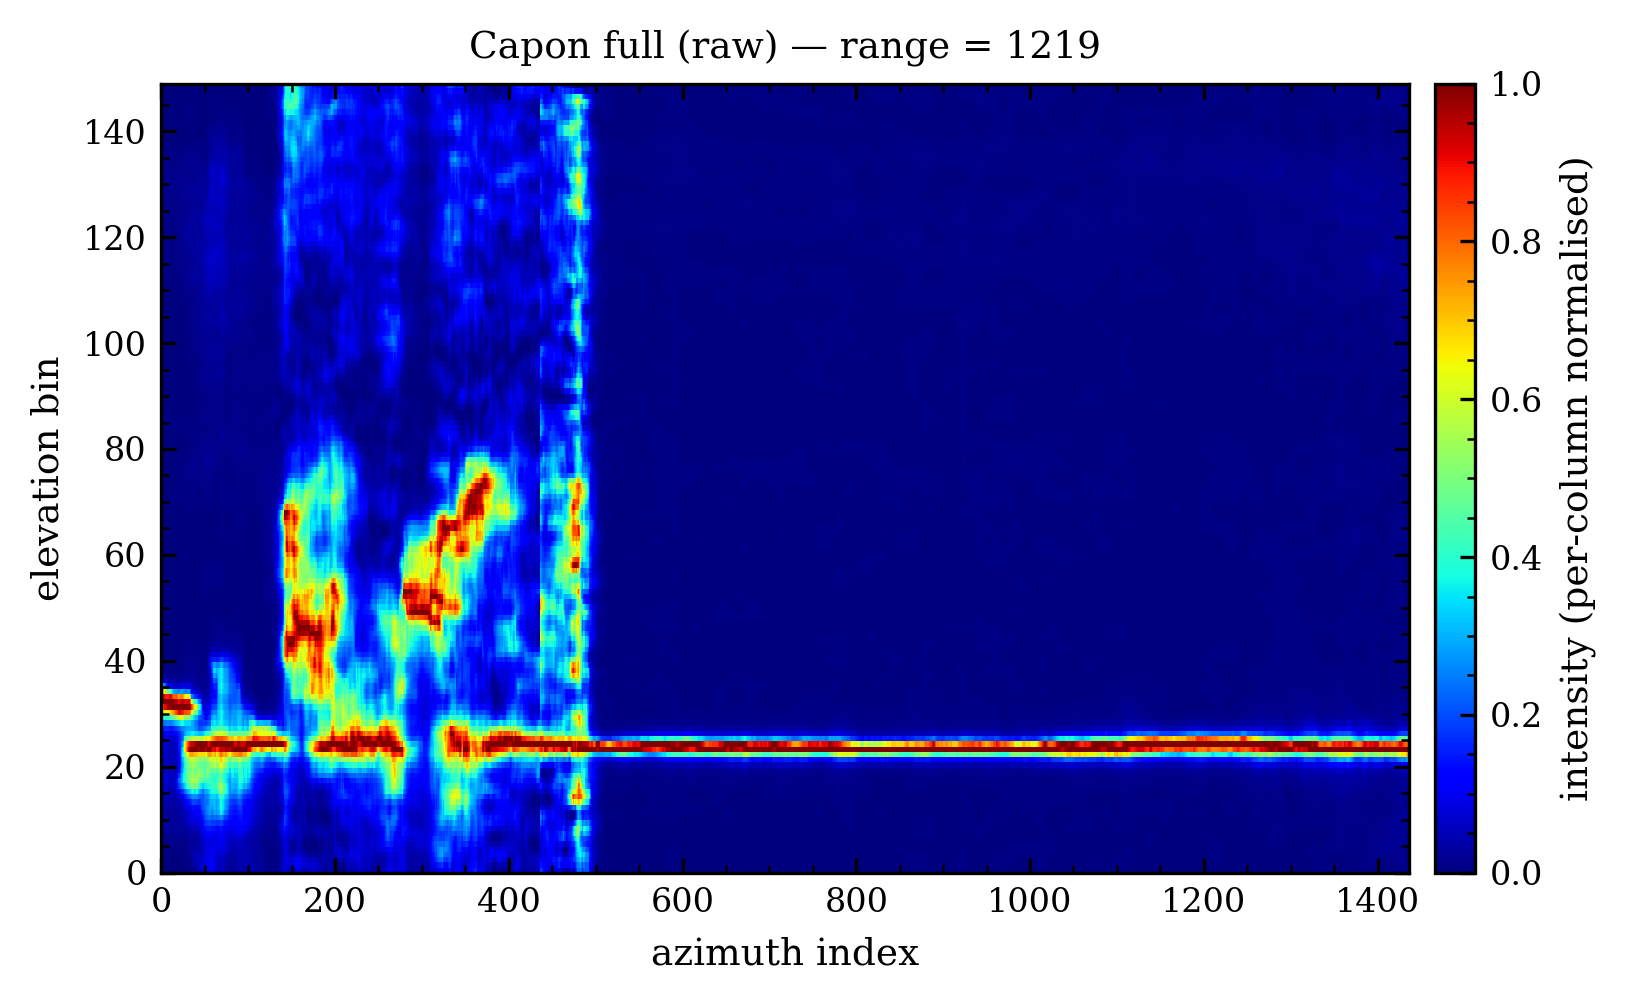
\includegraphics[width=\linewidth]{../figures/K2/dual_k2_ratio/cube_slices-90-10/cube_slices/az0331_rg1219/range_full_normalized.png}
    \end{minipage}\hspace{3pt}%
    \begin{minipage}[t]{0.345\textwidth}
      \centering
      {\small\textbf{\textcolor{good}{GT (Gaussian)}}}\\[3pt]
      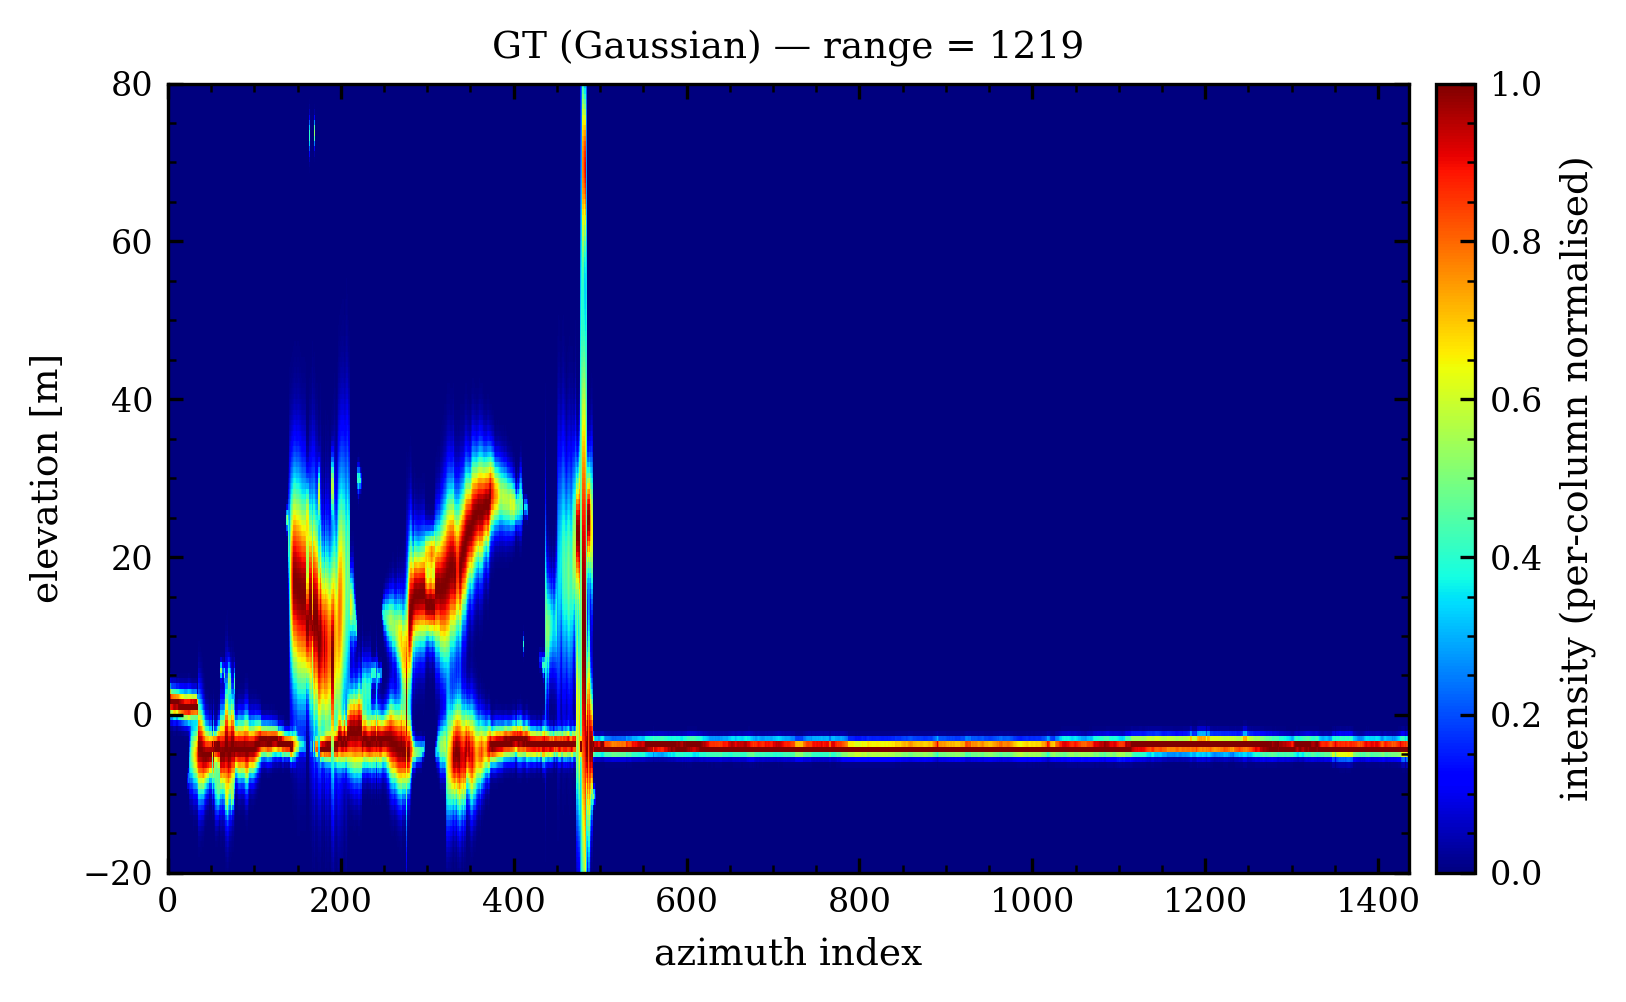
\includegraphics[width=\linewidth]{../figures/K2/dual_k2_ratio/cube_slices-90-10/cube_slices/az0331_rg1219/range_gt_normalized.png}
    \end{minipage}\hspace{3pt}%
    \begin{minipage}[t]{0.345\textwidth}
      \centering
      {\small\textbf{\textcolor{accent}{90--10 prediction}}}\\[3pt]
      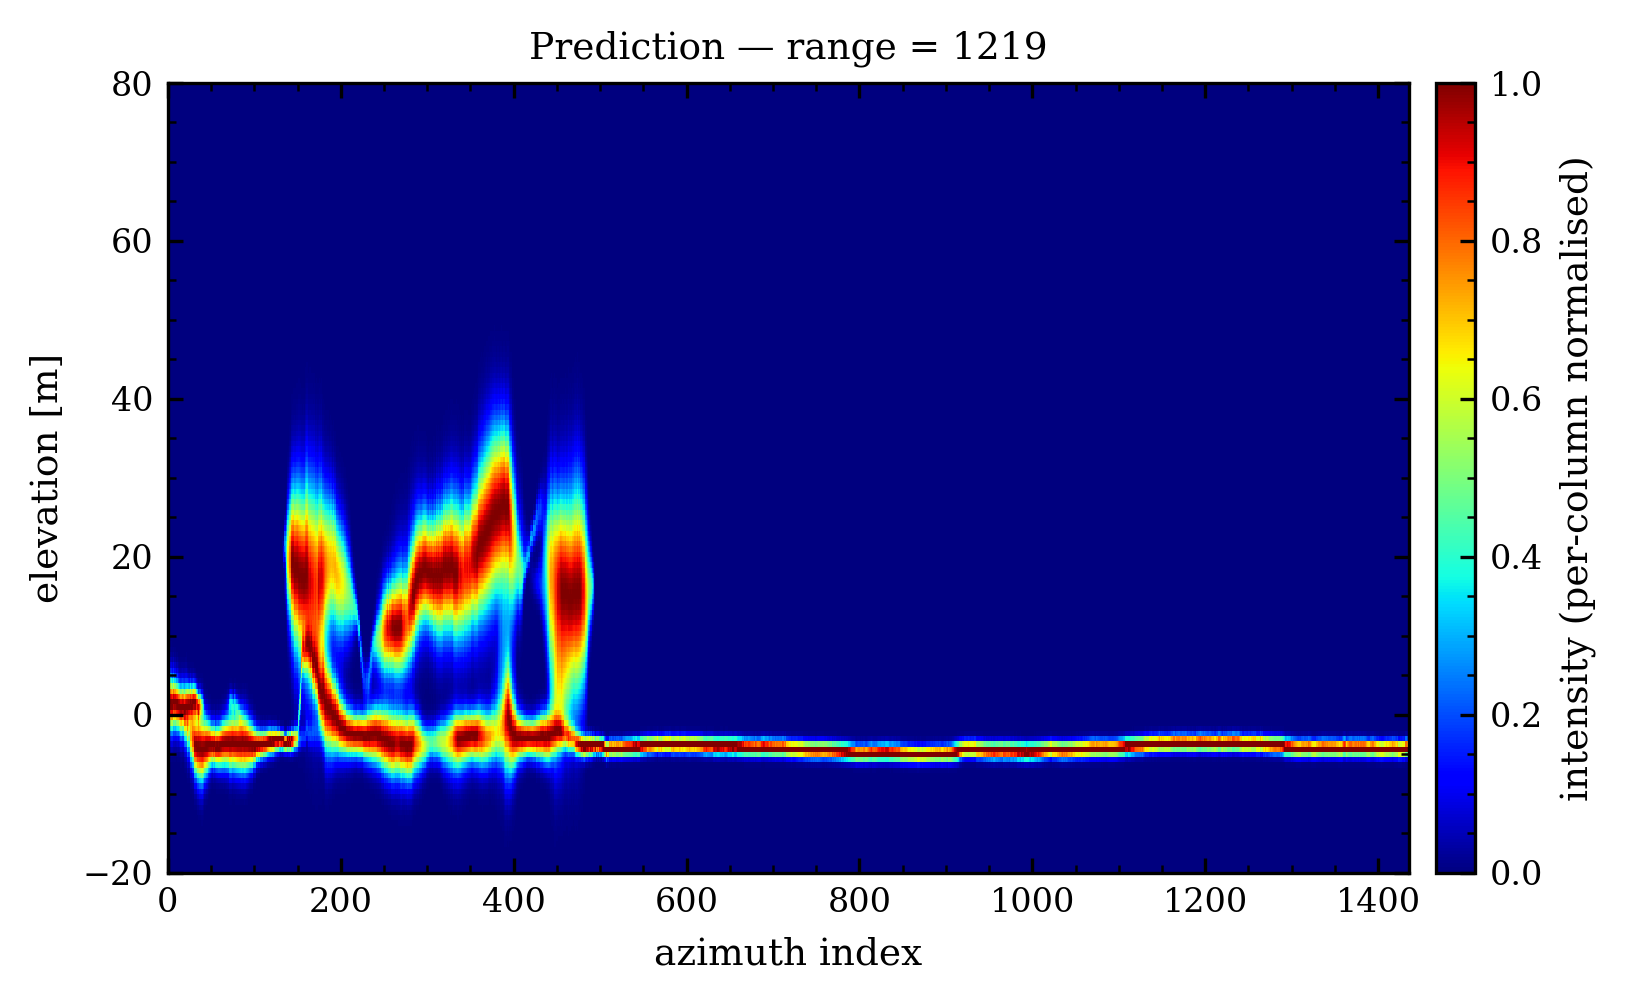
\includegraphics[width=\linewidth]{../figures/K2/dual_k2_ratio/cube_slices-90-10/cube_slices/az0331_rg1219/range_pred_normalized.png}
    \end{minipage}}
  \vspace{7pt}
  \parbox{0.90\textwidth}{\scriptsize\color{soft} Constant-range cut at $\mathrm{rg}=1219$, per-column normalised. The tomogram splits the scene before any fit: canopy clutter out to azimuth ${\approx}500$, then a single clean ground line to the swath edge. Label and prediction both follow that split, and the prediction holds the ground line at ${\approx}-4$\,m across the whole flat half. Its vegetated half comes out as broad smooth lobes where the label is filamentary --- the patch CNN regularises across neighbouring azimuths. The single-column GT streak at azimuth ${\approx}480$ sits on the tomogram's bright edge column but does not reach the prediction. Tomogram in elevation bins, the two mixture panels in metres.\par}
\end{frame}

% ---------------------------------------------------------------- 25x Ratio 90-10 slices: layered canopy
\begin{frame}{The 90--10 cube --- layered canopy over a continuous ground return}
  \centering
  \makebox[\textwidth][c]{%
    \begin{minipage}[t]{0.345\textwidth}
      \centering
      {\small\textbf{\textcolor{soft}{full-tomogram}}}\\[3pt]
      
\includegraphics[width=\linewidth]{../figures/K2/dual_k2_ratio/cube_slices-90-10/cube_slices/az1298_rg3230/range_full_normalized.png}
    \end{minipage}\hspace{3pt}%
    \begin{minipage}[t]{0.345\textwidth}
      \centering
      {\small\textbf{\textcolor{good}{GT (Gaussian)}}}\\[3pt]
      
\includegraphics[width=\linewidth]{../figures/K2/dual_k2_ratio/cube_slices-90-10/cube_slices/az1298_rg3230/range_gt_normalized.png}
    \end{minipage}\hspace{3pt}%
    \begin{minipage}[t]{0.345\textwidth}
      \centering
      {\small\textbf{\textcolor{accent}{90--10 prediction}}}\\[3pt]
      
\includegraphics[width=\linewidth]{../figures/K2/dual_k2_ratio/cube_slices-90-10/cube_slices/az1298_rg3230/range_pred_normalized.png}
    \end{minipage}}
  \vspace{7pt}
  \parbox{0.90\textwidth}{\scriptsize\color{soft} Constant-range cut at $\mathrm{rg}=3230$, per-column normalised. Two layers over roughly the first $850$ azimuths in all three panels: a ground return near $-6$\,m under vegetation at $15$--$25$\,m. The prediction keeps the separation, and the raised patch at azimuth $1130$--$1220$, where the return lifts to about $0$\,m before dropping back, shows in the tomogram, the label and the prediction alike. The thin GT column at azimuth ${\approx}790$ reaching past $60$\,m is cut short in the prediction --- isolated single-column towers are the failure mode these cuts keep showing. Tomogram in elevation bins, the two mixture panels in metres.\par}
\end{frame}

% ---------------------------------------------------------------- 25y Ratio 90-10 slices: dense canopy
\begin{frame}{The 90--10 cube --- dense canopy with a bare corridor}
  \centering
  \makebox[\textwidth][c]{%
    \begin{minipage}[t]{0.345\textwidth}
      \centering
      {\small\textbf{\textcolor{soft}{full-tomogram}}}\\[3pt]
      
\includegraphics[width=\linewidth]{../figures/K2/dual_k2_ratio/cube_slices-90-10/cube_slices/az1069_rg3466/range_full_normalized.png}
    \end{minipage}\hspace{3pt}%
    \begin{minipage}[t]{0.345\textwidth}
      \centering
      {\small\textbf{\textcolor{good}{GT (Gaussian)}}}\\[3pt]
      
\includegraphics[width=\linewidth]{../figures/K2/dual_k2_ratio/cube_slices-90-10/cube_slices/az1069_rg3466/range_gt_normalized.png}
    \end{minipage}\hspace{3pt}%
    \begin{minipage}[t]{0.345\textwidth}
      \centering
      {\small\textbf{\textcolor{accent}{90--10 prediction}}}\\[3pt]
      
\includegraphics[width=\linewidth]{../figures/K2/dual_k2_ratio/cube_slices-90-10/cube_slices/az1069_rg3466/range_pred_normalized.png}
    \end{minipage}}
  \vspace{7pt}
  \parbox{0.90\textwidth}{\scriptsize\color{soft} Constant-range cut at $\mathrm{rg}=3466$, per-column normalised: the densest of the four. Vegetation from azimuth $0$ to ${\approx}580$ and again from ${\approx}950$ out to the swath edge, with a bare corridor between them where only the ground return near $-7$\,m survives; the tomogram carries the same corridor. The prediction puts both blocks and the corridor in place and holds the sharp canopy wall at azimuth ${\approx}580$. Two costs: it picks the canopy back up at azimuth ${\approx}985$ against the label's ${\approx}955$, and the ${\approx}60$\,m point return near azimuth $1145$, visible in the tomogram as well as in the label, is missing. Tomogram in elevation bins, the two mixture panels in metres.\par}
\end{frame}


\act{VI \ \ Physics-constrained losses}{five terms \; $\cdot$ \; curriculum \; $\cdot$ \; \textcolor{soft}{results pending}}

% ---------------------------------------------------------------- 34 Why constrain
\begin{frame}{Why constrain the solution space}
  \small
  \begin{itemize}
    \item The labels are classical fits: the network's ceiling is the label quality ---
          and Act IV showed the network happily leans on statistical shortcuts.
    \item Physics terms restrict predictions to profiles \textbf{consistent with the SAR
          signal model}:
    \begin{itemize}
      \item today --- as a regularizer: physical quantities recomputed from the predicted
            profile must match those of the GT profile;
      \item next --- as self-supervision against the \emph{measured} covariance itself,
            removing the label ceiling entirely.
    \end{itemize}
    \item Five terms implemented and theory-tested; every one differentiable end-to-end
          through the Gaussian-mixture curve reconstruction.
  \end{itemize}
\end{frame}

% ---------------------------------------------------------------- 35 Forward operator
\begin{frame}{The shared forward operator}
  \small
  All terms use the vertical wavenumber and the steering matrix on the elevation grid:
  \[
    \boxed{\;k_z^{(i)} = \frac{4\pi\, b_i}{\lambda\, r_0\, s}, \qquad
    A_{in} = e^{\,j\, k_z^{(i)}\, \xi_n}\;}
  \]
  \begin{itemize}
    \item Geometry resolved from campaign track parameters --- not nominal defaults:
          per-pass perpendicular baselines, look angle, slant range.
    \item \textbf{Per-pixel $k_z$ field} for range/azimuth-varying geometry, built at
          preprocessing and threaded dataset $\to$ trainer $\to$ loss.
    \item Steering sign settled empirically ($+k_z$: median peak error 0.67\,m, within
          one Rayleigh cell).
  \end{itemize}
\end{frame}

% ---------------------------------------------------------------- 36 Data-consistency terms
\begin{frame}{Data-consistency terms (the ranked top two)}
  \setlength{\abovedisplayskip}{3pt}
  \setlength{\belowdisplayskip}{3pt}
  \begin{columns}[T]
    \begin{column}{0.46\textwidth}
      \begin{minipage}[t][0.78\textheight][s]{\linewidth}
      \centering
      \textbf{Coherence re-synthesis}\\[1pt]
      {\footnotesize\color{soft} coherence domain}
      \par\vfill
      \[
        \gamma_P(k_z^{(i)}) = \frac{\sum_n P(\xi_n)\, e^{j k_z^{(i)} \xi_n}}{\sum_n P(\xi_n)}
      \]
      \[
        \ell_{\text{coh}} = \Big\langle \tfrac{1}{N_s}\textstyle\sum_i
          \big| \gamma_P(k_z^{(i)}) - \gamma_T(k_z^{(i)}) \big|^2 \Big\rangle
      \]
      \par\vfill
      \begin{tikzpicture}[scale=0.70]
        \draw[->,soft] (-0.05,0) -- (3.55,0) node[right,font=\tiny]{$k_z^{(i)}$};
        \draw[->,soft] (0,-0.05) -- (0,1.55) node[above,font=\tiny]{$|\gamma|$};
        \draw[accent,semithick,domain=0.05:3.3,samples=60,smooth] plot (\x,{1.3*exp(-\x*\x/3.2)});
        \foreach \x/\d in {0.35/0.12, 0.9/-0.10, 1.45/0.11, 2.0/-0.09, 2.55/0.10, 3.05/-0.08} {
          \draw[good!70,thin] (\x,{1.3*exp(-\x*\x/3.2)}) -- (\x,{1.3*exp(-\x*\x/3.2)+\d});
          \fill[good] (\x,{1.3*exp(-\x*\x/3.2)+\d}) circle (1.5pt);
        }
      \end{tikzpicture}
      \\[4pt]
      {\scriptsize \textcolor{accent}{$\gamma_P$ from the predicted mixture} pulled onto
       \textcolor{good}{the target coherences}, baseline by baseline.}
      \par\vfill
      {\footnotesize Cloude 2006 (PCT); same Fourier kernel as gamma-Net (Qian et al.).}
      \end{minipage}
    \end{column}
    \begin{column}{0.02\textwidth}
      \centering
      \textcolor{soft!40}{\rule{0.4pt}{0.74\textheight}}
    \end{column}
    \begin{column}{0.46\textwidth}
      \begin{minipage}[t][0.78\textheight][s]{\linewidth}
      \centering
      \textbf{Covariance matching}\\[1pt]
      {\footnotesize\color{soft} covariance domain}
      \par\vfill
      \[
        \mathbf{R}[P] = \mathbf{A}\,\mathrm{diag}(P)\,\mathbf{A}^{H} \Delta\xi
      \]
      \[
        \ell_{\text{cov}} = \Big\langle
          \tfrac{\| \mathbf{R}[P] - \mathbf{R}[T] \|_F^2}{\| \mathbf{R}[T] \|_F^2} \Big\rangle
      \]
      \par\vfill
      \begin{tikzpicture}[scale=1.2]
        \foreach \i/\j/\c in {0/2/70,1/2/35,2/2/15,0/1/35,1/1/70,2/1/35,0/0/15,1/0/35,2/0/70}
          \fill[accent!\c] (\i*0.34,\j*0.34) rectangle ++(0.32,0.32);
        \draw[soft,thin] (-0.02,-0.02) rectangle (1.02,1.02);
        \node[font=\scriptsize,anchor=north] at (0.5,-0.1) {$\mathbf{R}[P]$};
        \draw[{Stealth[length=1.5mm]}-{Stealth[length=1.5mm]},accent,semithick] (1.35,0.5) -- (2.05,0.5);
        \node[font=\scriptsize,text=accent,anchor=south] at (1.7,0.58) {$\|\cdot\|_F$};
        \begin{scope}[shift={(2.4,0)}]
          \foreach \i/\j/\c in {0/2/60,1/2/40,2/2/20,0/1/40,1/1/60,2/1/28,0/0/20,1/0/28,2/0/60}
            \fill[good!\c] (\i*0.34,\j*0.34) rectangle ++(0.32,0.32);
          \draw[soft,thin] (-0.02,-0.02) rectangle (1.02,1.02);
          \node[font=\scriptsize,anchor=north] at (0.5,-0.1) {$\mathbf{R}[T]$};
        \end{scope}
      \end{tikzpicture}
      \\[4pt]
      {\scriptsize \textcolor{accent}{Synthesised} vs \textcolor{good}{target} covariance ---
       structure and relative scale, entry by entry.}
      \par\vfill
      {\footnotesize COMET (Ottersten, Stoica, Roy 1998); TomoSAR: Cros \& Ferro-Famil 2025;
       CS fidelity: Berenger et al. 2023.}
      \end{minipage}
    \end{column}
  \end{columns}
\end{frame}

% ---------------------------------------------------------------- 37a Descriptor terms
\begin{frame}{Descriptor terms: moments and total power}
  \setlength{\abovedisplayskip}{3pt}
  \setlength{\belowdisplayskip}{3pt}
  \begin{columns}[T]
    \begin{column}{0.46\textwidth}
      \centering
      \textbf{Moments}\\[1pt]
      {\footnotesize\color{soft} mass \; $\cdot$ \; phase-centre $\bar z$ \; $\cdot$ \; spread $\sigma_z$}
      \\[6pt]
      \[
        m = \textstyle\sum_n P(\xi_n)\,\Delta\xi
      \]
      \[
        \bar z = \tfrac{\sum_n \xi_n P(\xi_n)}{\sum_n P(\xi_n)}, \qquad
        \sigma_z^2 = \tfrac{\sum_n (\xi_n-\bar z)^2 P(\xi_n)}{\sum_n P(\xi_n)}
      \]
      \vspace{15pt}
      \begin{tikzpicture}[scale=0.9]
        \draw[->,soft] (-0.05,0) -- (4.35,0) node[right,font=\scriptsize]{$z$};
        \draw[->,soft] (0,-0.05) -- (0,1.75) node[above,font=\scriptsize]{$P(z)$};
        \fill[accent!10] plot[domain=0.05:4.15,samples=80,smooth]
          (\x,{1.3*exp(-(\x-1.3)^2/(2*0.38*0.38))+0.55*exp(-(\x-2.9)^2/(2*0.5*0.5))})
          -- (4.15,0) -- (0.05,0) -- cycle;
        \begin{scope}
          \clip plot[domain=0.05:4.15,samples=80,smooth]
            (\x,{1.3*exp(-(\x-1.3)^2/(2*0.38*0.38))+0.55*exp(-(\x-2.9)^2/(2*0.5*0.5))})
            -- (4.15,0) -- (0.05,0) -- cycle;
          \draw[accent!30,very thin,step=0.16] (0,0) grid (4.2,1.6);
        \end{scope}
        \draw[accent,thick,domain=0.05:4.15,samples=100,smooth]
          plot (\x,{1.3*exp(-(\x-1.3)^2/(2*0.38*0.38))+0.55*exp(-(\x-2.9)^2/(2*0.5*0.5))});
        \draw[ink,dotted,thick] (1.8,0) -- (1.8,1.5);
        \node[font=\scriptsize,text=ink,anchor=north] at (1.8,-0.06) {$\bar z$};
        \draw[{Stealth[length=1.4mm]}-{Stealth[length=1.4mm]},soft,thin] (0.95,1.28) -- (2.65,1.28);
        \node[font=\scriptsize,text=ink,anchor=south] at (1.8,1.33) {$\sigma_z$};
      \end{tikzpicture}
      \\[2pt]
      {\scriptsize Centroid and spread are bias-robust \emph{ratios}
       (Cros \& Ferro-Famil 2025).}
    \end{column}
    \begin{column}{0.02\textwidth}
      \centering
      \textcolor{soft!40}{\rule{0.4pt}{0.58\textheight}}
    \end{column}
    \begin{column}{0.46\textwidth}
      \centering
      \textbf{Total power}\\[1pt]
      {\footnotesize\color{soft} the one absolute-power quantity}
      \\[6pt]
      \[
        P_{\text{tot}}[\,\cdot\,] = \textstyle\sum_n (\,\cdot\,)(\xi_n)\,\Delta\xi
      \]
      \[
        \ell_{\text{pow}} = \Big\langle \big( P_{\text{tot}}[P] - P_{\text{tot}}[T] \big)^2 \Big\rangle
      \]
      \vspace{15pt}
      \begin{tikzpicture}[scale=0.9]
        \draw[->,soft] (-0.05,0) -- (4.35,0) node[right,font=\scriptsize]{scene position};
        \draw[->,soft] (0,-0.05) -- (0,1.75) node[above,font=\scriptsize]{$P_{\text{tot}}$};
        \draw[soft,densely dashed] (0,1.4) -- (4.15,1.4);
        \node[font=\tiny,text=soft,anchor=south west] at (0.08,1.43) {true level};
        \draw[accent,thick,domain=0.05:4.15,samples=120,smooth]
          plot (\x,{0.82+0.26*sin(\x*110)+0.12*sin(\x*260+70)});
        \node[font=\tiny,text=accent,anchor=west] at (0.25,0.28)
          {$P_{\text{tot}}[T]$ --- bias varies with the scene};
        \draw[{Stealth[length=1.3mm]}-{Stealth[length=1.3mm]},soft,thin] (3.9,1.07) -- (3.9,1.4);
        \node[font=\tiny,text=ink,anchor=east] at (3.83,1.2) {$\sim$2\,dB};
      \end{tikzpicture}
      \\[2pt]
      {\scriptsize The target $P_{\text{tot}}[T]$ is not the true power: its bias moves with
       scene content (Lopez-Dekker \& Mallorqui 2010) --- the loss would imprint that bias.}
    \end{column}
  \end{columns}
\end{frame}

% ---------------------------------------------------------------- 37b Estimator cycle
\begin{frame}{The estimator-cycle term: Capon cycle}
  \setlength{\abovedisplayskip}{4pt}
  \setlength{\belowdisplayskip}{4pt}
  \small
  Push the prediction through the \emph{same estimator} that produced the ground truth:
  \[
    \hat T_P(\xi_n) = \big( \mathbf{a}^{H}(\xi_n)
      (\mathbf{R}[P] + \epsilon\bar\sigma\mathbf{I})^{-1} \mathbf{a}(\xi_n) \big)^{-1}
  \]
  \vspace{8pt}
  \begin{center}
  \begin{tikzpicture}
    \draw[soft,thin] (0,0) -- (1.8,0);
    \draw[accent,thick,domain=0.08:1.72,samples=70,smooth]
      plot (\x,{0.62*exp(-(\x-0.6)^2/(2*0.11*0.11))+0.38*exp(-(\x-1.2)^2/(2*0.13*0.13))});
    \node[font=\scriptsize,text=soft,anchor=north] at (0.9,-0.12) {predicted profile $P$};
    \draw[flow] (1.95,0.45) -- (3.9,0.45);
    \node[font=\scriptsize,text=soft,anchor=south] at (2.92,0.58)
      {$\mathbf{R}[P]=\mathbf{A}\,\mathrm{diag}(P)\,\mathbf{A}^{H}$};
    \begin{scope}[shift={(4.1,-0.06)}]
      \foreach \i/\j/\c in {0/2/70, 1/2/35, 2/2/15, 0/1/35, 1/1/70, 2/1/35, 0/0/15, 1/0/35, 2/0/70}
        \fill[accent!\c] (\i*0.34,\j*0.34) rectangle ++(0.32,0.32);
      \draw[soft,thin] (-0.02,-0.02) rectangle (1.02,1.02);
    \end{scope}
    \node[font=\scriptsize,text=soft,anchor=north] at (4.61,-0.12) {synthesised covariance};
    \draw[flow] (5.27,0.45) -- (7.95,0.45);
    \node[font=\scriptsize,text=soft,anchor=south,align=center] at (6.61,0.58)
      {Capon --- \emph{the same estimator}\\\emph{that produced the GT}};
    \draw[soft,thin] (8.1,0) -- (9.9,0);
    \draw[accent,thick,domain=8.18:9.82,samples=70,smooth]
      plot (\x,{0.50*exp(-(\x-8.7)^2/(2*0.19*0.19))+0.30*exp(-(\x-9.3)^2/(2*0.22*0.22))});
    \node[font=\scriptsize,text=soft,anchor=north,align=center] at (9.0,-0.12)
      {re-estimated\\spectrum $\hat T_P$};
    \draw[{Stealth[length=1.6mm]}-{Stealth[length=1.6mm]},accent,semithick] (10.05,0.45) -- (10.75,0.45);
    \node[font=\scriptsize,text=accent,anchor=south] at (10.4,0.55) {$\ell$};
    \draw[soft,thin] (10.9,0) -- (12.7,0);
    \draw[good,thick,domain=10.98:12.62,samples=70,smooth]
      plot (\x,{0.50*exp(-(\x-11.5)^2/(2*0.19*0.19))+0.30*exp(-(\x-12.1)^2/(2*0.22*0.22))});
    \node[font=\scriptsize,text=soft,anchor=north,align=center] at (11.8,-0.12)
      {Capon tomogram $T$\\(ground truth)};
    \draw[accent!70,dashed,-{Stealth[length=1.8mm]}] (11.8,-0.95) -- (0.9,-0.95) -- (0.9,-0.62);
    \node[font=\scriptsize,text=accent!80,anchor=north] at (6.35,-1.02)
      {gradient --- differentiable end-to-end};
  \end{tikzpicture}
  \end{center}
  \vspace{6pt}
  \begin{itemize}
    \item Absorbs the Capon bias and the PSF \textbf{by construction}.
    \item Costs an $N_s\times N_s$ solve per pixel --- the most expensive of the five.
  \end{itemize}
  \vspace{2pt}
  {\scriptsize\color{soft} Cycle-consistency lineage: Yaman 2020, Lu 2021,
   Vella \& Mota 2020, Angermann 2023.\par}
\end{frame}

% ---------------------------------------------------------------- 38 Curriculum motivation
\begin{frame}{Why the physics terms need a curriculum}
  \small
  The physics terms are the most sensitive consumers of the reconstructed profile ---
  and at random initialisation they see only noise:
  \begin{center}
  \begin{tikzpicture}[node distance=9mm]
    \node[gate, text width=27mm] (init) {\textbf{untrained network}\\{\tiny predicted profiles are noise}};
    \node[gate, text width=40mm, right=of init] (fwd)  {\textbf{physics forward operators}\\{\tiny $\mathbf{R}[P]$, Capon solve --- \mbox{ill-conditioned} on unphysical profiles}};
    \node[gate, text width=34mm, right=of fwd]  (grad) {\textbf{huge, unstable losses}\\{\tiny gradients drown the useful signal}};
    \draw[flow] (init) -- (fwd);
    \draw[flow] (fwd) -- (grad);
  \end{tikzpicture}
  \end{center}
  \vspace{-2pt}
  \begin{center}
  \begin{tikzpicture}
    \fill[black!4] (0,0)   rectangle (3.6,2.7);
    \fill[good!6]  (3.6,0) rectangle (11.6,2.7);
    \node[font=\tiny, text=soft, anchor=north west]           at (0.08,2.62) {\textbf{warmup stage} --- param-L1 only};
    \node[font=\tiny, text=good!80!black, anchor=north west]  at (3.68,2.62) {\textbf{complete stage} --- full composite, physics terms enter};
    \node[font=\tiny\itshape, text=soft, anchor=north east]   at (11.52,2.62) {schematic};
    \draw[soft, dashed] (3.6,-0.35) -- (3.6,2.7);
    \node[font=\tiny, text=soft, anchor=north] at (3.6,-0.4) {swap (default epoch 15)};
    \draw[->, soft] (0,0) -- (12.0,0)  node[right, font=\scriptsize] {epoch};
    \draw[->, soft] (0,0) -- (0,2.85)  node[above, font=\scriptsize] {loss};
    \draw[accent!35, very thin] plot coordinates
      {(0.20,1.94) (0.23,1.80) (0.27,1.83) (0.30,1.83) (0.34,1.94) (0.37,2.14) (0.41,2.08)
       (0.44,1.96) (0.48,1.86) (0.51,1.90) (0.54,1.92) (0.58,1.84) (0.61,1.91) (0.65,1.84)
       (0.68,2.00) (0.72,2.08) (0.75,2.13) (0.79,2.02) (0.82,2.05) (0.85,2.01) (0.89,1.97)
       (0.92,1.95) (0.96,1.86) (0.99,1.80) (1.03,1.96) (1.06,1.96) (1.10,2.00) (1.13,2.09)
       (1.16,1.91) (1.20,1.89) (1.23,1.96) (1.27,2.02) (1.30,1.99) (1.34,2.09) (1.37,2.08)
       (1.41,1.95) (1.44,1.90) (1.47,2.03) (1.51,2.07) (1.54,1.89) (1.58,2.07) (1.61,2.10)
       (1.65,2.19) (1.68,2.09) (1.72,2.04) (1.75,1.94) (1.78,2.20) (1.82,2.12) (1.85,2.22)
       (1.89,2.08) (1.92,2.08) (1.96,1.92) (1.99,1.95) (2.03,2.08) (2.06,1.96) (2.09,2.09)
       (2.13,2.10) (2.16,1.99) (2.20,1.98) (2.23,1.97) (2.27,2.00) (2.30,1.98) (2.34,1.94)
       (2.37,1.97) (2.40,1.92) (2.44,1.87) (2.47,1.95) (2.51,2.07) (2.54,1.93) (2.58,1.99)
       (2.61,1.96) (2.65,1.92) (2.68,2.05) (2.71,2.01) (2.75,2.16) (2.78,2.05) (2.82,2.08)
       (2.85,2.05) (2.89,1.99) (2.92,2.07) (2.96,2.05) (2.99,2.10) (3.02,2.08) (3.06,1.97)
       (3.09,2.00) (3.13,2.03) (3.16,2.12) (3.20,2.01) (3.23,2.02) (3.27,1.89) (3.30,2.01)
       (3.33,1.94) (3.37,1.83) (3.40,1.92) (3.44,2.34) (3.47,2.19) (3.51,2.01) (3.54,1.95)
       (3.58,1.89) (3.61,1.97) (3.64,1.93) (3.68,1.91) (3.71,2.02) (3.74,1.96) (3.78,2.03)
       (3.81,1.94) (3.84,1.88) (3.88,2.34) (3.91,2.31) (3.94,2.13) (3.98,2.03) (4.01,2.02)
       (4.04,2.03) (4.08,2.03) (4.11,2.18) (4.14,2.01) (4.18,1.88) (4.21,1.85) (4.25,1.80)
       (4.28,1.96) (4.31,2.04) (4.35,1.94) (4.38,1.85) (4.41,1.88) (4.45,2.05) (4.48,1.78)
       (4.51,2.25) (4.55,2.01) (4.58,2.07) (4.61,1.93) (4.65,1.91) (4.68,1.81) (4.71,1.80)
       (4.75,2.00) (4.78,2.34) (4.81,2.17) (4.85,1.98) (4.88,2.12) (4.91,1.98) (4.95,1.95)
       (4.98,1.94) (5.01,1.93) (5.05,1.84) (5.08,1.88) (5.11,1.91) (5.15,2.04) (5.18,2.15)
       (5.21,2.05) (5.25,1.93) (5.28,1.93) (5.32,1.88) (5.35,1.84) (5.38,1.88) (5.42,1.81)
       (5.45,1.92) (5.48,1.91) (5.52,1.94) (5.55,1.92) (5.58,1.86) (5.62,1.80) (5.65,1.84)
       (5.68,1.83) (5.72,1.89) (5.75,1.90) (5.78,1.79) (5.82,1.85) (5.85,1.76) (5.88,1.77)
       (5.92,1.81) (5.95,1.68) (5.98,1.79) (6.02,1.85) (6.05,1.86) (6.08,1.84) (6.12,1.84)
       (6.15,1.78) (6.18,1.81) (6.22,1.80) (6.25,1.85) (6.28,2.12) (6.32,2.01) (6.35,1.95)
       (6.39,1.87) (6.42,1.84) (6.45,1.91) (6.49,1.76) (6.52,1.86) (6.55,1.89) (6.59,1.91)
       (6.62,1.93) (6.65,1.86) (6.69,1.85) (6.72,1.92) (6.75,1.94) (6.79,1.93) (6.82,1.78)
       (6.85,1.87) (6.89,1.98) (6.92,2.02) (6.95,1.98) (6.99,1.81) (7.02,1.92) (7.05,1.89)
       (7.09,1.68) (7.12,1.80) (7.15,1.71) (7.19,1.68) (7.22,1.72) (7.25,1.90) (7.29,1.87)
       (7.32,1.90) (7.35,2.04) (7.39,2.11) (7.42,2.00) (7.46,1.93) (7.49,1.81) (7.52,1.79)
       (7.56,1.87) (7.59,1.92) (7.62,1.92) (7.66,2.00) (7.69,1.89) (7.72,1.89) (7.76,1.96)
       (7.79,1.98) (7.82,2.04) (7.86,2.02) (7.89,2.34) (7.92,2.23) (7.96,1.98) (7.99,1.80)
       (8.02,1.90) (8.06,1.89) (8.09,1.93) (8.12,1.78) (8.16,1.82) (8.19,1.81) (8.22,1.79)
       (8.26,1.66) (8.29,1.76) (8.32,1.91) (8.36,1.96) (8.39,1.90) (8.42,1.92) (8.46,1.99)
       (8.49,1.74) (8.52,1.82) (8.56,1.93) (8.59,2.34) (8.63,2.33) (8.66,2.24) (8.69,2.09)
       (8.73,2.06) (8.76,2.08) (8.79,1.98) (8.83,1.97) (8.86,2.05) (8.89,2.18) (8.93,2.08)
       (8.96,2.03) (8.99,2.02) (9.03,2.12) (9.06,2.06) (9.09,2.15) (9.13,2.00) (9.16,1.98)
       (9.19,1.97) (9.23,2.05) (9.26,2.12) (9.29,1.94) (9.33,1.89) (9.36,1.97) (9.39,1.94)
       (9.43,1.84) (9.46,2.01) (9.49,2.06) (9.53,2.08) (9.56,2.02) (9.59,2.11) (9.63,2.05)
       (9.66,2.14) (9.70,2.01) (9.73,1.95) (9.76,2.01) (9.80,1.96) (9.83,2.06) (9.86,2.08)
       (9.90,1.99) (9.93,2.02) (9.96,2.01) (10.00,2.11) (10.03,2.03) (10.06,2.01) (10.10,2.14)
       (10.13,2.29) (10.16,2.34) (10.20,2.24) (10.23,2.18) (10.26,2.26) (10.30,2.17) (10.33,2.04)
       (10.36,2.07) (10.40,2.11) (10.43,2.03) (10.46,1.91) (10.50,1.87) (10.53,2.02) (10.56,1.99)
       (10.60,2.02) (10.63,2.07) (10.66,2.14) (10.70,2.09) (10.73,2.14) (10.77,2.04) (10.80,2.04)
       (10.83,1.98) (10.87,2.13) (10.90,2.12) (10.93,2.05) (10.97,2.04) (11.00,2.05) (11.03,2.14)
       (11.07,1.99) (11.10,1.96) (11.13,1.99) (11.17,2.26) (11.20,2.28) (11.23,2.19) (11.27,2.22)
       (11.30,2.34)};
    \draw[accent, semithick] plot coordinates
      {(0.20,1.94) (0.34,1.92) (0.48,1.94) (0.61,1.93) (0.75,1.95) (0.89,1.96) (1.03,1.95)
       (1.16,1.96) (1.30,1.96) (1.44,1.97) (1.58,1.98) (1.72,2.00) (1.85,2.03) (1.99,2.03)
       (2.13,2.03) (2.27,2.02) (2.40,2.01) (2.54,2.00) (2.68,1.99) (2.82,2.01) (2.96,2.02)
       (3.09,2.02) (3.23,2.03) (3.37,2.00) (3.51,2.03) (3.64,2.01) (3.78,2.00) (3.91,2.03)
       (4.04,2.03) (4.18,2.03) (4.31,2.01) (4.45,1.99) (4.58,2.00) (4.71,1.97) (4.85,2.00)
       (4.98,2.00) (5.11,1.98) (5.25,1.99) (5.38,1.97) (5.52,1.95) (5.65,1.93) (5.78,1.91)
       (5.92,1.89) (6.05,1.87) (6.18,1.86) (6.32,1.88) (6.45,1.88) (6.59,1.88) (6.72,1.88)
       (6.85,1.88) (6.99,1.89) (7.12,1.88) (7.25,1.85) (7.39,1.88) (7.52,1.88) (7.66,1.89)
       (7.79,1.90) (7.92,1.96) (8.06,1.94) (8.19,1.92) (8.32,1.89) (8.46,1.90) (8.59,1.92)
       (8.73,1.97) (8.86,1.98) (8.99,2.00) (9.13,2.02) (9.26,2.02) (9.39,2.00) (9.53,2.00)
       (9.66,2.02) (9.80,2.01) (9.93,2.02) (10.06,2.02) (10.20,2.07) (10.33,2.09) (10.46,2.08)
       (10.60,2.06) (10.73,2.07) (10.87,2.06) (11.00,2.06) (11.13,2.05) (11.27,2.09)};
    \node[font=\tiny, text=accent, anchor=north east] at (11.3,1.52)
      {\textbf{physics from epoch 0} --- gradients drown, never converges};
    \draw[soft!45, very thin] plot coordinates
      {(0.20,1.50) (0.23,1.50) (0.25,1.46) (0.28,1.39) (0.31,1.35) (0.33,1.30) (0.36,1.31)
       (0.38,1.39) (0.41,1.34) (0.44,1.30) (0.46,1.32) (0.49,1.33) (0.52,1.31) (0.54,1.24)
       (0.57,1.24) (0.60,1.27) (0.62,1.18) (0.65,1.16) (0.67,1.07) (0.70,1.03) (0.73,0.97)
       (0.75,1.01) (0.78,0.98) (0.81,1.03) (0.83,1.06) (0.86,1.07) (0.89,0.96) (0.91,0.97)
       (0.94,1.00) (0.96,1.02) (0.99,0.96) (1.02,0.97) (1.04,0.95) (1.07,0.94) (1.10,1.01)
       (1.12,0.98) (1.15,0.99) (1.18,1.03) (1.20,1.00) (1.23,1.00) (1.25,1.00) (1.28,1.00)
       (1.31,0.95) (1.33,0.96) (1.36,1.02) (1.39,0.94) (1.41,0.98) (1.44,0.98) (1.47,0.95)
       (1.49,1.03) (1.52,1.04) (1.54,0.97) (1.57,0.96) (1.60,0.98) (1.62,0.96) (1.65,0.97)
       (1.68,0.96) (1.70,0.97) (1.73,1.01) (1.76,0.96) (1.78,0.95) (1.81,0.92) (1.83,0.92)
       (1.86,0.87) (1.89,0.86) (1.91,0.86) (1.94,0.90) (1.97,0.93) (1.99,0.87) (2.02,0.85)
       (2.04,0.88) (2.07,0.81) (2.10,0.81) (2.12,0.82) (2.15,0.87) (2.18,0.89) (2.20,0.87)
       (2.23,0.86) (2.26,0.85) (2.28,0.90) (2.31,0.87) (2.33,0.86) (2.36,0.87) (2.39,0.86)
       (2.41,0.85) (2.44,0.81) (2.47,0.82) (2.49,0.81) (2.52,0.85) (2.55,0.87) (2.57,0.86)
       (2.60,0.88) (2.62,0.85) (2.65,0.88) (2.68,0.87) (2.70,0.88) (2.73,0.82) (2.76,0.83)
       (2.78,0.78) (2.81,0.72) (2.84,0.74) (2.86,0.73) (2.89,0.76) (2.91,0.84) (2.94,0.81)
       (2.97,0.79) (2.99,0.80) (3.02,0.82) (3.05,0.81) (3.07,0.81) (3.10,0.83) (3.13,0.84)
       (3.15,0.80) (3.18,0.80) (3.20,0.80) (3.23,0.77) (3.26,0.79) (3.28,0.77) (3.31,0.81)
       (3.34,0.81) (3.36,0.81) (3.39,0.79) (3.42,0.79) (3.44,0.73) (3.47,0.71) (3.49,0.75)
       (3.52,0.69) (3.55,0.75) (3.57,0.71) (3.60,0.75)};
    \draw[soft, semithick] plot coordinates
      {(0.20,1.50) (0.28,1.48) (0.36,1.44) (0.44,1.41) (0.52,1.39) (0.60,1.35) (0.67,1.29)
       (0.75,1.21) (0.83,1.16) (0.91,1.12) (0.99,1.08) (1.07,1.05) (1.15,1.03) (1.23,1.03)
       (1.31,1.01) (1.39,1.00) (1.47,0.99) (1.54,1.00) (1.62,0.99) (1.70,0.98) (1.78,0.98)
       (1.86,0.96) (1.94,0.94) (2.02,0.92) (2.10,0.90) (2.18,0.89) (2.26,0.88) (2.33,0.88)
       (2.41,0.87) (2.49,0.86) (2.57,0.86) (2.65,0.86) (2.73,0.86) (2.81,0.84) (2.89,0.81)
       (2.97,0.81) (3.05,0.81) (3.13,0.82) (3.20,0.81) (3.28,0.80) (3.36,0.80) (3.44,0.80)
       (3.52,0.77) (3.60,0.76)};
    \draw[good, dotted, thick] (3.60,0.76) -- (3.60,1.29);
    \draw[good!40, very thin] plot coordinates
      {(3.60,1.29) (3.63,1.32) (3.66,1.28) (3.70,1.11) (3.73,1.20) (3.76,1.27) (3.79,1.21)
       (3.83,1.14) (3.86,1.09) (3.89,1.00) (3.92,1.07) (3.95,1.01) (3.99,0.99) (4.02,0.93)
       (4.05,0.89) (4.08,0.82) (4.12,0.92) (4.15,0.91) (4.18,0.97) (4.21,0.95) (4.24,0.89)
       (4.28,0.87) (4.31,0.84) (4.34,0.84) (4.37,0.83) (4.41,0.81) (4.44,0.75) (4.47,0.73)
       (4.50,0.84) (4.53,0.80) (4.57,0.75) (4.60,0.78) (4.63,0.85) (4.66,0.77) (4.70,0.76)
       (4.73,0.74) (4.76,0.67) (4.79,0.73) (4.82,0.74) (4.86,0.75) (4.89,0.72) (4.92,0.75)
       (4.95,0.72) (4.99,0.72) (5.02,0.68) (5.05,0.64) (5.08,0.72) (5.11,0.70) (5.15,0.72)
       (5.18,0.72) (5.21,0.70) (5.24,0.68) (5.28,0.71) (5.31,0.70) (5.34,0.69) (5.37,0.69)
       (5.40,0.73) (5.44,0.75) (5.47,0.74) (5.50,0.71) (5.53,0.65) (5.57,0.69) (5.60,0.72)
       (5.63,0.70) (5.66,0.71) (5.69,0.72) (5.73,0.73) (5.76,0.74) (5.79,0.70) (5.82,0.74)
       (5.86,0.67) (5.89,0.69) (5.92,0.69) (5.95,0.71) (5.98,0.75) (6.02,0.76) (6.05,0.69)
       (6.08,0.62) (6.11,0.65) (6.15,0.61) (6.18,0.61) (6.21,0.63) (6.24,0.58) (6.27,0.52)
       (6.31,0.55) (6.34,0.56) (6.37,0.56) (6.40,0.57) (6.44,0.55) (6.47,0.52) (6.50,0.53)
       (6.53,0.52) (6.56,0.49) (6.60,0.53) (6.63,0.54) (6.66,0.56) (6.69,0.54) (6.73,0.53)
       (6.76,0.51) (6.79,0.50) (6.82,0.52) (6.85,0.51) (6.89,0.54) (6.92,0.55) (6.95,0.62)
       (6.98,0.56) (7.02,0.59) (7.05,0.58) (7.08,0.57) (7.11,0.53) (7.14,0.52) (7.18,0.55)
       (7.21,0.55) (7.24,0.55) (7.27,0.54) (7.31,0.58) (7.34,0.57) (7.37,0.50) (7.40,0.49)
       (7.43,0.45) (7.47,0.38) (7.50,0.41) (7.53,0.48) (7.56,0.49) (7.59,0.47) (7.63,0.46)
       (7.66,0.51) (7.69,0.52) (7.72,0.53) (7.76,0.53) (7.79,0.53) (7.82,0.55) (7.85,0.56)
       (7.88,0.56) (7.92,0.52) (7.95,0.54) (7.98,0.51) (8.01,0.55) (8.05,0.51) (8.08,0.51)
       (8.11,0.51) (8.14,0.48) (8.17,0.53) (8.21,0.57) (8.24,0.54) (8.27,0.56) (8.30,0.56)
       (8.34,0.48) (8.37,0.49) (8.40,0.50) (8.43,0.50) (8.46,0.48) (8.50,0.48) (8.53,0.48)
       (8.56,0.52) (8.59,0.53) (8.63,0.52) (8.66,0.56) (8.69,0.53) (8.72,0.51) (8.75,0.46)
       (8.79,0.52) (8.82,0.54) (8.85,0.55) (8.88,0.56) (8.92,0.55) (8.95,0.54) (8.98,0.53)
       (9.01,0.51) (9.04,0.51) (9.08,0.55) (9.11,0.55) (9.14,0.54) (9.17,0.51) (9.21,0.49)
       (9.24,0.54) (9.27,0.54) (9.30,0.53) (9.33,0.51) (9.37,0.48) (9.40,0.48) (9.43,0.51)
       (9.46,0.49) (9.50,0.49) (9.53,0.48) (9.56,0.49) (9.59,0.45) (9.62,0.45) (9.66,0.44)
       (9.69,0.48) (9.72,0.46) (9.75,0.48) (9.79,0.52) (9.82,0.51) (9.85,0.49) (9.88,0.49)
       (9.91,0.49) (9.95,0.47) (9.98,0.48) (10.01,0.54) (10.04,0.52) (10.08,0.51) (10.11,0.47)
       (10.14,0.49) (10.17,0.45) (10.20,0.43) (10.24,0.48) (10.27,0.46) (10.30,0.49) (10.33,0.53)
       (10.37,0.53) (10.40,0.53) (10.43,0.57) (10.46,0.54) (10.49,0.51) (10.53,0.47) (10.56,0.47)
       (10.59,0.52) (10.62,0.53) (10.66,0.50) (10.69,0.47) (10.72,0.46) (10.75,0.47) (10.78,0.47)
       (10.82,0.48) (10.85,0.49) (10.88,0.48) (10.91,0.48) (10.95,0.48) (10.98,0.48) (11.01,0.49)
       (11.04,0.54) (11.07,0.54) (11.11,0.53) (11.14,0.47) (11.17,0.48) (11.20,0.43) (11.24,0.41)
       (11.27,0.45) (11.30,0.47)};
    \draw[good, semithick] plot coordinates
      {(3.60,1.29) (3.73,1.27) (3.86,1.23) (3.99,1.16) (4.12,1.07) (4.24,1.02) (4.37,0.96)
       (4.50,0.90) (4.63,0.86) (4.76,0.82) (4.89,0.79) (5.02,0.76) (5.15,0.74) (5.28,0.73)
       (5.40,0.72) (5.53,0.71) (5.66,0.71) (5.79,0.71) (5.92,0.71) (6.05,0.72) (6.18,0.68)
       (6.31,0.64) (6.44,0.62) (6.56,0.58) (6.69,0.57) (6.82,0.55) (6.95,0.55) (7.08,0.56)
       (7.21,0.55) (7.34,0.56) (7.47,0.52) (7.59,0.50) (7.72,0.50) (7.85,0.52) (7.98,0.52)
       (8.11,0.52) (8.24,0.52) (8.37,0.52) (8.50,0.51) (8.63,0.51) (8.75,0.51) (8.88,0.52)
       (9.01,0.53) (9.14,0.53) (9.27,0.53) (9.40,0.52) (9.53,0.51) (9.66,0.49) (9.79,0.49)
       (9.91,0.49) (10.04,0.50) (10.17,0.49) (10.30,0.48) (10.43,0.50) (10.56,0.50) (10.69,0.50)
       (10.82,0.49) (10.95,0.49) (11.07,0.50) (11.20,0.49)};
    \node[font=\tiny, text=good, anchor=south east] at (11.3,0.68)
      {\textbf{physics at the swap} --- enter tamed, composite converges};
  \end{tikzpicture}
  \end{center}
\end{frame}

% ---------------------------------------------------------------- 39 Swap mechanics + status
\begin{frame}{Swap mechanics, calibration --- and status}
  \small
  Each detail is an anticipated failure mode:
  \begin{itemize}
    \item \textbf{Resets at the swap}: LR schedule origin, LR warmup, Adam moments,
          early-stopping counters --- optimizer state calibrated to the old loss is stale
          under the new one.
    \item \textbf{Checkpoint-baseline reset}: best-loss tracking restarts across the
          non-comparable loss scales --- otherwise the pre-swap best could never be
          beaten.
    \item \textbf{Stage inheritance}: the complete stage is the base configuration,
          warmup a derived pre-phase materialised at launch --- the stages cannot drift.
    \item \textbf{Loss-scale probe}: every active term run at unit weight over probe
          batches, IQR-filtered, folded into the per-term weights --- physics terms enter
          at calibrated magnitude, not guessed weights.
  \end{itemize}
  \begin{block}{\small Status}
    \small Implemented, SAR-theory-verified, geometry wired end-to-end ---
    the single-term $K{=}2$ sweep is in (next frames); the Capon-cycle arm,
    the most expensive of the five, is still queued.
  \end{block}
\end{frame}

% ---------------------------------------------------------------- 39b Physics sweep results
\begin{frame}{The physics sweep at $K{=}2$ --- every term rides low, the scale terms collapse high}
    \centering
  \scriptsize
  \renewcommand{\arraystretch}{0.70}
  \setlength{\tabcolsep}{2.2pt}
  \renewcommand{\seedtag}{phyA}
  \begin{tabular}{@{}l ccccccccc@{}}
    \toprule
    & \multicolumn{2}{c}{reconstruction} & \multicolumn{7}{c@{}}{detection (matched)} \\
    \cmidrule(lr){2-3}\cmidrule(l){4-10}
    objective & curve $R^2$ $\uparrow$ & cos med $\uparrow$ & prec.\ $\uparrow$ & recall $\uparrow$ & F1 $\uparrow$ & exact $\uparrow$ & under $\downarrow$ & over $\downarrow$ & peak p95 $\downarrow$ \\
    \midrule
    param-L1 $+$ cos & \seedpm{0.747}{.006} & \seedpm{0.965}{.004} & \seedpm{0.895}{.008} & \seedpm{0.901}{.001} & \seedpm{0.898}{.004} & \seedpm{0.908}{.007} & \seedpm{0.041}{.003} & \seedpm{0.051}{.009} & \seedpm{4.7}{.0} \\
    \addlinespace
    \multicolumn{10}{@{}l}{\emph{$+$ coherence re-synthesis}} \\
    \quad $w{=}0.01$ & \seedpm{0.752}{.004} & \seedpm{0.966}{.002} & \seedpm{0.895}{.006} & \seedpm{0.902}{.001} & \seedpm{0.898}{.003} & \seedpm{0.910}{.002} & \seedpm{0.040}{.004} & \seedpm{0.050}{.005} & \seedpm{4.7}{.0} \\
    \quad $w{=}0.05$ & \seedpm{0.752}{.006} & \seedpm{0.966}{.001} & \seedpm{0.893}{.005} & \seedpm{0.902}{.001} & \seedpm{0.898}{.002} & \seedpm{0.911}{.003} & \seedpm{0.039}{.003} & \seedpm{0.051}{.004} & \seedpm{4.7}{.0} \\
    \quad $w{=}0.25$ & \seedpm{\hlval{good}{0.755}}{.007} & \seedpm{0.966}{.002} & \seedpm{0.892}{.009} & \seedpm{0.903}{.002} & \seedpm{0.897}{.004} & \seedpm{0.909}{.005} & \seedpm{0.038}{.005} & \seedpm{0.053}{.010} & \seedpm{4.7}{.0} \\
    \quad $w{=}0.5$ & \seedpm{0.748}{.009} & \seedpm{0.965}{.003} & \seedpm{0.886}{.013} & \seedpm{0.903}{.001} & \seedpm{0.895}{.007} & \seedpm{0.911}{.010} & \seedpm{0.032}{.006} & \seedpm{0.057}{.014} & \seedpm{4.7}{.0} \\
    \quad $w{=}1$ & \seedpm{0.751}{.008} & \seedpm{0.966}{.002} & \seedpm{0.870}{.045} & \seedpm{0.903}{.001} & \seedpm{0.886}{.024} & \seedpm{0.885}{.063} & \seedpm{\hlval{good}{\textbf{0.032}}}{.005} & \seedpm{\hlval{accent}{0.083}}{.068} & \seedpm{4.7}{.0} \\
    \addlinespace
    \multicolumn{10}{@{}l}{\emph{$+$ covariance matching}} \\
    \quad $w{=}0.01$ & \seedpm{0.752}{.001} & \seedpm{0.965}{.002} & \seedpm{0.896}{.005} & \seedpm{0.901}{.001} & \seedpm{0.898}{.003} & \seedpm{0.906}{.004} & \seedpm{0.043}{.001} & \seedpm{0.051}{.005} & \seedpm{4.7}{.0} \\
    \quad $w{=}0.05$ & \seedpm{0.748}{.001} & \seedpm{0.966}{.002} & \seedpm{0.899}{.005} & \seedpm{0.902}{.001} & \seedpm{0.900}{.002} & \seedpm{0.909}{.004} & \seedpm{0.043}{.002} & \seedpm{0.048}{.005} & \seedpm{4.7}{.0} \\
    \quad $w{=}0.25$ & \seedpm{0.738}{.004} & \seedpm{0.966}{.002} & \seedpm{0.896}{.006} & \seedpm{0.899}{.002} & \seedpm{0.898}{.003} & \seedpm{0.902}{.008} & \seedpm{0.045}{.002} & \seedpm{0.053}{.008} & \seedpm{4.7}{.0} \\
    \quad $w{=}0.5$ & \seedpm{\hlval{accent}{0.727}}{.011} & \seedpm{0.965}{.002} & \seedpm{0.900}{.001} & \seedpm{0.898}{.002} & \seedpm{0.899}{.001} & \seedpm{0.907}{.003} & \seedpm{0.046}{.003} & \seedpm{0.047}{.001} & \seedpm{4.7}{.0} \\
    \quad $w{=}1$ & \seedpm{\hlval{accent}{0.723}}{.006} & \seedpm{0.965}{.001} & \seedpm{0.899}{.005} & \seedpm{0.899}{.002} & \seedpm{0.899}{.002} & \seedpm{0.903}{.003} & \seedpm{0.047}{.004} & \seedpm{0.050}{.006} & \seedpm{4.7}{.0} \\
    \addlinespace
    \multicolumn{10}{@{}l}{\emph{$+$ moments}} \\
    \quad $w{=}0.01$ & \seedpm{0.753}{.003} & \seedpm{0.966}{.002} & \seedpm{0.895}{.006} & \seedpm{0.902}{.001} & \seedpm{0.898}{.003} & \seedpm{0.910}{.004} & \seedpm{0.040}{.005} & \seedpm{0.050}{.006} & \seedpm{4.7}{.0} \\
    \quad $w{=}0.05$ & \seedpm{0.755}{.002} & \seedpm{0.966}{.002} & \seedpm{0.896}{.005} & \seedpm{0.902}{.001} & \seedpm{0.899}{.002} & \seedpm{0.910}{.004} & \seedpm{0.041}{.004} & \seedpm{0.049}{.005} & \seedpm{4.7}{.0} \\
    \quad $w{=}0.25$ & \seedpm{0.751}{.002} & \seedpm{0.965}{.002} & \seedpm{0.897}{.004} & \seedpm{0.901}{.001} & \seedpm{0.899}{.002} & \seedpm{0.908}{.003} & \seedpm{0.044}{.000} & \seedpm{0.049}{.004} & \seedpm{4.7}{.0} \\
    \quad $w{=}0.5$ & \seedpm{0.750}{.004} & \seedpm{0.966}{.002} & \seedpm{0.898}{.003} & \seedpm{0.900}{.001} & \seedpm{0.899}{.001} & \seedpm{0.909}{.001} & \seedpm{0.044}{.002} & \seedpm{0.047}{.003} & \seedpm{4.7}{.0} \\
    \quad $w{=}1$ & \seedpm{0.746}{.005} & \seedpm{0.966}{.001} & \seedpm{0.897}{.003} & \seedpm{0.901}{.001} & \seedpm{0.899}{.002} & \seedpm{0.908}{.003} & \seedpm{0.043}{.001} & \seedpm{0.049}{.003} & \seedpm{4.7}{.0} \\
    \addlinespace
    \multicolumn{10}{@{}l}{\emph{$+$ total power}} \\
    \quad $w{=}0.01$ & \seedpm{0.752}{.003} & \seedpm{0.965}{.002} & \seedpm{0.896}{.005} & \seedpm{0.902}{.001} & \seedpm{0.899}{.002} & \seedpm{0.910}{.004} & \seedpm{0.041}{.004} & \seedpm{0.049}{.005} & \seedpm{4.7}{.0} \\
    \quad $w{=}0.05$ & \seedpm{0.751}{.005} & \seedpm{0.966}{.001} & \seedpm{0.897}{.003} & \seedpm{0.900}{.001} & \seedpm{0.899}{.002} & \seedpm{0.908}{.002} & \seedpm{0.044}{.001} & \seedpm{0.048}{.002} & \seedpm{4.7}{.0} \\
    \quad $w{=}0.25$ & \seedpm{0.747}{.003} & \seedpm{0.965}{.001} & \seedpm{0.898}{.003} & \seedpm{0.900}{.001} & \seedpm{0.899}{.001} & \seedpm{0.908}{.004} & \seedpm{0.044}{.003} & \seedpm{0.049}{.004} & \seedpm{4.7}{.0} \\
    \quad $w{=}0.5$ & \seedpm{\hlval{accent}{0.737}}{.015} & \seedpm{0.965}{.002} & \seedpm{0.900}{.005} & \seedpm{0.899}{.002} & \seedpm{0.899}{.003} & \seedpm{0.905}{.006} & \seedpm{0.048}{.004} & \seedpm{0.047}{.006} & \seedpm{4.7}{.0} \\
    \quad $w{=}1$ & \seedpm{\hlval{accent}{0.724}}{.020} & \seedpm{0.963}{.005} & \seedpm{0.902}{.003} & \seedpm{0.898}{.005} & \seedpm{0.900}{.001} & \seedpm{0.907}{.003} & \seedpm{0.049}{.007} & \seedpm{\textbf{0.044}}{.004} & \seedpm{4.8}{.3} \\
    \bottomrule
    \end{tabular}
  \par\vspace{1pt}
  \parbox{0.97\textwidth}{\tiny\color{soft} \textbf{runs}: dual UNet-skip trunks $\cdot$ set-pred $\cdot$ Hungarian
   $\cdot$ $K{=}2$ $\cdot$ presence A $\cdot$ full norm ladder $\cdot$ hv flips
   $\cdot$ patch $64{\times}32$ $\cdot$ fixed routing (full stack $\to$ both
   trunks) $\cdot$ parity twins. Row $=$ loss $(\text{param-L1}+0.5\,\text{cos}+w\,\text{phys})/(1.5+w)$,
   one physics term per arm; param-L1 $+$ cos $=$ the no-physics reference. Five
   seeded replicas per arm, cells mean $\pm$ seed std; held-out test, $5.0$\,M px.
   Val losses do not compare across arms (different composites); curve MAE / PSNR /
   SSIM stay flat outside the collapse arms (next frames); peak p95 is pinned at
   4.7. \textbf{bold} $=$ best in column, marked only where best and worst differ
   by more than $5\%$. \textcolor{good}{Green}: coherence
   $w{=}0.25$ takes the best curve $R^2$; at $w{=}1$ its gate trades misses for
   false alarms (under 0.041 $\to$ 0.032, over 0.051 $\to$ 0.083; seed lottery:
   precision $\pm$.045, exact $\pm$.063). \textcolor{accent}{Red} $=$
   absolute-scale collapse past $w{=}0.25$ (covariance, total power). cos med: median per-pixel cosine to GT; peak p95: 95th pct of
   the per-pixel peak error.\par}
\end{frame}

% ---------------------------------------------------------------- 39c Physics detection by count
\begin{frame}{The $K{=}2$ physics detection by scatterer count --- the set is untouched at every weight}
    \centering
  \scriptsize
  \renewcommand{\arraystretch}{0.73}
  \setlength{\tabcolsep}{5pt}
  \renewcommand{\seedtag}{phyB}
  \begin{tabular}{@{}l cccccccc@{}}
    \toprule
    & \multicolumn{3}{c}{precision $\uparrow$} & \multicolumn{3}{c}{recall $\uparrow$} & \multicolumn{2}{c@{}}{count acc $\mid$ pred $k$ $\uparrow$} \\
    \cmidrule(lr){2-4}\cmidrule(lr){5-7}\cmidrule(l){8-9}
    objective & all & $k{=}1$ & $k{=}2$ & all & $k{=}1$ & $k{=}2$ & $k{=}1$ & $k{=}2$ \\
    \midrule
    param-L1 $+$ cos & \seedpm{0.895}{.008} & \seedpm{0.935}{.010} & \seedpm{0.828}{.006} & \seedpm{0.901}{.001} & \seedpm{0.999}{.000} & \seedpm{0.763}{.002} & \seedpm{0.944}{.004} & \seedpm{0.814}{.024} \\
    \addlinespace
    \multicolumn{9}{@{}l}{\emph{$+$ coherence re-synthesis}} \\
    \quad $w{=}0.01$ & \seedpm{0.895}{.006} & \seedpm{0.935}{.006} & \seedpm{0.828}{.006} & \seedpm{0.902}{.001} & \seedpm{0.999}{.000} & \seedpm{0.765}{.001} & \seedpm{0.945}{.005} & \seedpm{0.815}{.012} \\
    \quad $w{=}0.05$ & \seedpm{0.893}{.005} & \seedpm{0.935}{.005} & \seedpm{0.826}{.005} & \seedpm{0.902}{.001} & \seedpm{0.999}{.000} & \seedpm{0.765}{.002} & \seedpm{0.947}{.004} & \seedpm{0.814}{.011} \\
    \quad $w{=}0.25$ & \seedpm{0.892}{.009} & \seedpm{0.932}{.011} & \seedpm{0.826}{.006} & \seedpm{0.903}{.002} & \seedpm{0.999}{.000} & \seedpm{0.766}{.004} & \seedpm{0.948}{.006} & \seedpm{0.808}{.023} \\
    \quad $w{=}0.5$ & \seedpm{0.886}{.013} & \seedpm{0.928}{.016} & \seedpm{0.818}{.010} & \seedpm{0.903}{.001} & \seedpm{0.999}{.000} & \seedpm{\hlval{good}{0.767}}{.003} & \seedpm{0.955}{.008} & \seedpm{0.803}{.033} \\
    \quad $w{=}1$ & \seedpm{0.870}{.045} & \seedpm{\hlval{accent}{0.902}}{.067} & \seedpm{0.818}{.009} & \seedpm{0.903}{.001} & \seedpm{0.999}{.000} & \seedpm{\hlval{good}{0.768}}{.001} & \seedpm{0.954}{.002} & \seedpm{\hlval{accent}{0.755}}{.122} \\
    \addlinespace
    \multicolumn{9}{@{}l}{\emph{$+$ covariance matching}} \\
    \quad $w{=}0.01$ & \seedpm{0.896}{.005} & \seedpm{0.935}{.006} & \seedpm{0.831}{.004} & \seedpm{0.901}{.001} & \seedpm{0.999}{.000} & \seedpm{0.761}{.002} & \seedpm{0.943}{.003} & \seedpm{0.812}{.016} \\
    \quad $w{=}0.05$ & \seedpm{0.899}{.005} & \seedpm{0.938}{.006} & \seedpm{0.834}{.003} & \seedpm{0.902}{.001} & \seedpm{0.999}{.000} & \seedpm{0.763}{.003} & \seedpm{0.943}{.002} & \seedpm{0.819}{.015} \\
    \quad $w{=}0.25$ & \seedpm{0.896}{.006} & \seedpm{0.932}{.009} & \seedpm{0.835}{.002} & \seedpm{0.899}{.002} & \seedpm{0.999}{.000} & \seedpm{0.758}{.005} & \seedpm{0.944}{.003} & \seedpm{0.803}{.023} \\
    \quad $w{=}0.5$ & \seedpm{0.900}{.001} & \seedpm{0.939}{.002} & \seedpm{0.836}{.002} & \seedpm{0.898}{.002} & \seedpm{0.999}{.000} & \seedpm{0.755}{.005} & \seedpm{0.943}{.005} & \seedpm{0.820}{.005} \\
    \quad $w{=}1$ & \seedpm{0.899}{.005} & \seedpm{0.936}{.007} & \seedpm{0.837}{.002} & \seedpm{0.899}{.002} & \seedpm{0.999}{.000} & \seedpm{0.756}{.005} & \seedpm{0.942}{.007} & \seedpm{0.812}{.015} \\
    \addlinespace
    \multicolumn{9}{@{}l}{\emph{$+$ moments}} \\
    \quad $w{=}0.01$ & \seedpm{0.895}{.006} & \seedpm{0.936}{.007} & \seedpm{0.827}{.007} & \seedpm{0.902}{.001} & \seedpm{0.999}{.000} & \seedpm{0.764}{.002} & \seedpm{0.945}{.006} & \seedpm{0.816}{.015} \\
    \quad $w{=}0.05$ & \seedpm{0.896}{.005} & \seedpm{0.937}{.006} & \seedpm{0.828}{.006} & \seedpm{0.902}{.001} & \seedpm{0.999}{.000} & \seedpm{0.764}{.003} & \seedpm{0.944}{.005} & \seedpm{0.817}{.015} \\
    \quad $w{=}0.25$ & \seedpm{0.897}{.004} & \seedpm{0.937}{.004} & \seedpm{0.831}{.004} & \seedpm{0.901}{.001} & \seedpm{0.999}{.000} & \seedpm{0.761}{.003} & \seedpm{0.941}{.001} & \seedpm{0.817}{.011} \\
    \quad $w{=}0.5$ & \seedpm{0.898}{.003} & \seedpm{0.939}{.004} & \seedpm{0.832}{.003} & \seedpm{0.900}{.001} & \seedpm{0.999}{.000} & \seedpm{0.761}{.003} & \seedpm{0.942}{.002} & \seedpm{0.821}{.009} \\
    \quad $w{=}1$ & \seedpm{0.897}{.003} & \seedpm{0.937}{.004} & \seedpm{0.832}{.003} & \seedpm{0.901}{.001} & \seedpm{0.999}{.000} & \seedpm{0.761}{.002} & \seedpm{0.943}{.001} & \seedpm{0.817}{.009} \\
    \addlinespace
    \multicolumn{9}{@{}l}{\emph{$+$ total power}} \\
    \quad $w{=}0.01$ & \seedpm{0.896}{.005} & \seedpm{0.937}{.006} & \seedpm{0.828}{.006} & \seedpm{0.902}{.001} & \seedpm{0.999}{.000} & \seedpm{0.763}{.001} & \seedpm{0.944}{.005} & \seedpm{0.818}{.013} \\
    \quad $w{=}0.05$ & \seedpm{0.897}{.003} & \seedpm{0.938}{.003} & \seedpm{0.831}{.004} & \seedpm{0.900}{.001} & \seedpm{0.999}{.000} & \seedpm{0.761}{.003} & \seedpm{0.941}{.001} & \seedpm{0.819}{.007} \\
    \quad $w{=}0.25$ & \seedpm{0.898}{.003} & \seedpm{0.937}{.004} & \seedpm{0.833}{.004} & \seedpm{0.900}{.001} & \seedpm{0.999}{.000} & \seedpm{0.761}{.003} & \seedpm{0.942}{.002} & \seedpm{0.817}{.011} \\
    \quad $w{=}0.5$ & \seedpm{0.900}{.005} & \seedpm{0.939}{.007} & \seedpm{0.834}{.003} & \seedpm{0.899}{.002} & \seedpm{0.999}{.000} & \seedpm{0.757}{.006} & \seedpm{0.937}{.006} & \seedpm{0.820}{.018} \\
    \quad $w{=}1$ & \seedpm{0.902}{.003} & \seedpm{0.943}{.005} & \seedpm{0.834}{.002} & \seedpm{0.898}{.005} & \seedpm{0.999}{.000} & \seedpm{0.755}{.011} & \seedpm{0.934}{.008} & \seedpm{\textbf{0.829}}{.009} \\
    \bottomrule
    \end{tabular}
  \par\vspace{2pt}
  \parbox{0.90\textwidth}{\tiny\color{soft} \textbf{runs}: dual UNet-skip trunks $\cdot$ set-pred $\cdot$ Hungarian
   $\cdot$ $K{=}2$ $\cdot$ presence A $\cdot$ full norm ladder $\cdot$ hv flips
   $\cdot$ patch $64{\times}32$ $\cdot$ fixed routing (full stack $\to$ both
   trunks) $\cdot$ parity twins. Row $=$ one physics term at weight $w$;
   param-L1 $+$ cos $=$ the no-physics reference. Five seeded replicas per arm,
   cells mean $\pm$ seed std; held-out test, $5.0$\,M px. All rows matched
   (Hungarian pairing); $k$ $=$ true scatterer count of the pixel. \textbf{bold}
   $=$ best in column, marked only where best and worst differ by more than $5\%$
   --- almost nothing clears it at any weight: the physics terms shape the profile,
   not the scatterer set. The exception is the high-weight coherence gate:
   \textcolor{good}{$k{=}2$ recall creeps up} (0.763 $\to$ 0.768) while
   \textcolor{accent}{the claimed pairs destabilise} ($k{=}1$ precision seed
   lottery $\pm$.067, pred $k{=}2$ accuracy $\pm$.122). Precision rewards
   under-prediction --- rank on recall. count acc $\mid$ pred $k$: share of pixels
   claiming exactly $k$ scatterers whose true count is $k$.\par}
\end{frame}

% ---------------------------------------------------------------- 39d Physics component errors
\begin{frame}{The $K{=}2$ physics component errors --- covariance buys position, coherence pays it}
    \centering
  \scriptsize
  \renewcommand{\arraystretch}{0.72}
  \setlength{\tabcolsep}{3pt}
  \renewcommand{\seedtag}{phyC}
  \begin{tabular}{@{}l ccccccccc@{}}
    \toprule
    & \multicolumn{3}{c}{$\mu$ MAE $\downarrow$} & \multicolumn{3}{c}{$\sigma$ MAE $\downarrow$} & \multicolumn{3}{c@{}}{$a$ MAE $\downarrow$} \\
    \cmidrule(lr){2-4}\cmidrule(lr){5-7}\cmidrule(l){8-10}
    objective & all & $k{=}1$ & $k{=}2$ & all & $k{=}1$ & $k{=}2$ & all & $k{=}1$ & $k{=}2$ \\
    \midrule
    param-L1 $+$ cos & \seedpm{1.71}{.07} & \seedpm{0.36}{.01} & \seedpm{3.78}{.14} & \seedpm{0.774}{.011} & \seedpm{0.193}{.002} & \seedpm{1.668}{.023} & \seedpm{0.182}{.004} & \seedpm{0.058}{.003} & \seedpm{0.373}{.006} \\
    \addlinespace
    \multicolumn{10}{@{}l}{\emph{$+$ coherence re-synthesis}} \\
    \quad $w{=}0.01$ & \seedpm{1.70}{.06} & \seedpm{0.35}{.01} & \seedpm{3.78}{.12} & \seedpm{0.770}{.009} & \seedpm{0.194}{.003} & \seedpm{1.654}{.024} & \seedpm{\textbf{0.180}}{.003} & \seedpm{\textbf{0.057}}{.002} & \seedpm{0.369}{.004} \\
    \quad $w{=}0.05$ & \seedpm{1.72}{.05} & \seedpm{0.35}{.01} & \seedpm{3.82}{.11} & \seedpm{0.779}{.014} & \seedpm{0.195}{.002} & \seedpm{1.673}{.035} & \seedpm{0.180}{.003} & \seedpm{0.057}{.003} & \seedpm{\textbf{0.369}}{.004} \\
    \quad $w{=}0.25$ & \seedpm{1.72}{.06} & \seedpm{0.35}{.00} & \seedpm{3.82}{.13} & \seedpm{0.778}{.011} & \seedpm{0.192}{.003} & \seedpm{1.675}{.016} & \seedpm{0.182}{.005} & \seedpm{0.058}{.004} & \seedpm{0.373}{.005} \\
    \quad $w{=}0.5$ & \seedpm{1.80}{.10} & \seedpm{0.35}{.01} & \seedpm{4.00}{.22} & \seedpm{0.804}{.017} & \seedpm{0.191}{.002} & \seedpm{1.730}{.033} & \seedpm{0.183}{.004} & \seedpm{0.058}{.003} & \seedpm{0.372}{.004} \\
    \quad $w{=}1$ & \seedpm{\hlval{accent}{1.81}}{.12} & \seedpm{0.35}{.00} & \seedpm{4.02}{.26} & \seedpm{\hlval{accent}{0.809}}{.020} & \seedpm{0.194}{.006} & \seedpm{1.737}{.035} & \seedpm{0.185}{.006} & \seedpm{0.061}{.008} & \seedpm{0.373}{.004} \\
    \addlinespace
    \multicolumn{10}{@{}l}{\emph{$+$ covariance matching}} \\
    \quad $w{=}0.01$ & \seedpm{1.66}{.04} & \seedpm{0.35}{.01} & \seedpm{3.70}{.09} & \seedpm{0.755}{.014} & \seedpm{0.192}{.004} & \seedpm{1.626}{.032} & \seedpm{0.182}{.003} & \seedpm{0.058}{.003} & \seedpm{0.374}{.004} \\
    \quad $w{=}0.05$ & \seedpm{\hlval{good}{1.65}}{.02} & \seedpm{0.35}{.01} & \seedpm{3.66}{.05} & \seedpm{0.754}{.007} & \seedpm{0.194}{.002} & \seedpm{1.620}{.017} & \seedpm{0.187}{.005} & \seedpm{0.061}{.004} & \seedpm{0.381}{.007} \\
    \quad $w{=}0.25$ & \seedpm{1.62}{.01} & \seedpm{0.34}{.01} & \seedpm{3.62}{.04} & \seedpm{0.725}{.011} & \seedpm{0.186}{.002} & \seedpm{\textbf{1.566}}{.024} & \seedpm{0.196}{.004} & \seedpm{0.065}{.004} & \seedpm{0.400}{.006} \\
    \quad $w{=}0.5$ & \seedpm{\textbf{1.61}}{.01} & \seedpm{0.34}{.01} & \seedpm{\textbf{3.61}}{.03} & \seedpm{\textbf{0.724}}{.014} & \seedpm{\textbf{0.186}}{.003} & \seedpm{1.567}{.035} & \seedpm{0.205}{.005} & \seedpm{0.069}{.004} & \seedpm{0.418}{.010} \\
    \quad $w{=}1$ & \seedpm{1.61}{.02} & \seedpm{0.35}{.01} & \seedpm{3.61}{.04} & \seedpm{0.728}{.018} & \seedpm{0.189}{.008} & \seedpm{1.575}{.039} & \seedpm{0.214}{.012} & \seedpm{0.071}{.005} & \seedpm{0.439}{.024} \\
    \addlinespace
    \multicolumn{10}{@{}l}{\emph{$+$ moments}} \\
    \quad $w{=}0.01$ & \seedpm{1.71}{.06} & \seedpm{0.35}{.01} & \seedpm{3.79}{.14} & \seedpm{0.772}{.017} & \seedpm{0.195}{.003} & \seedpm{1.657}{.041} & \seedpm{0.180}{.003} & \seedpm{0.057}{.002} & \seedpm{0.369}{.004} \\
    \quad $w{=}0.05$ & \seedpm{1.69}{.04} & \seedpm{0.35}{.01} & \seedpm{3.75}{.09} & \seedpm{0.771}{.018} & \seedpm{0.195}{.003} & \seedpm{1.657}{.043} & \seedpm{0.182}{.003} & \seedpm{0.058}{.003} & \seedpm{0.372}{.002} \\
    \quad $w{=}0.25$ & \seedpm{1.68}{.04} & \seedpm{0.35}{.01} & \seedpm{3.72}{.09} & \seedpm{0.763}{.005} & \seedpm{0.195}{.003} & \seedpm{1.643}{.015} & \seedpm{0.186}{.004} & \seedpm{0.060}{.003} & \seedpm{0.380}{.005} \\
    \quad $w{=}0.5$ & \seedpm{1.66}{.03} & \seedpm{0.35}{.01} & \seedpm{3.69}{.07} & \seedpm{0.759}{.007} & \seedpm{0.194}{.002} & \seedpm{1.634}{.016} & \seedpm{0.190}{.004} & \seedpm{0.062}{.004} & \seedpm{0.387}{.005} \\
    \quad $w{=}1$ & \seedpm{1.66}{.02} & \seedpm{0.35}{.01} & \seedpm{3.69}{.04} & \seedpm{0.760}{.008} & \seedpm{0.196}{.004} & \seedpm{1.633}{.012} & \seedpm{0.192}{.002} & \seedpm{0.063}{.003} & \seedpm{0.391}{.003} \\
    \addlinespace
    \multicolumn{10}{@{}l}{\emph{$+$ total power}} \\
    \quad $w{=}0.01$ & \seedpm{1.70}{.05} & \seedpm{0.35}{.01} & \seedpm{3.77}{.10} & \seedpm{0.771}{.019} & \seedpm{0.196}{.004} & \seedpm{1.656}{.045} & \seedpm{0.180}{.003} & \seedpm{0.057}{.003} & \seedpm{0.370}{.003} \\
    \quad $w{=}0.05$ & \seedpm{1.67}{.03} & \seedpm{0.35}{.00} & \seedpm{3.72}{.08} & \seedpm{0.761}{.005} & \seedpm{0.194}{.003} & \seedpm{1.639}{.015} & \seedpm{0.184}{.004} & \seedpm{0.059}{.004} & \seedpm{0.377}{.004} \\
    \quad $w{=}0.25$ & \seedpm{1.65}{.03} & \seedpm{0.35}{.01} & \seedpm{3.66}{.05} & \seedpm{0.753}{.011} & \seedpm{0.195}{.004} & \seedpm{1.619}{.016} & \seedpm{0.188}{.005} & \seedpm{0.060}{.005} & \seedpm{0.385}{.006} \\
    \quad $w{=}0.5$ & \seedpm{1.63}{.02} & \seedpm{0.35}{.01} & \seedpm{3.62}{.04} & \seedpm{0.762}{.022} & \seedpm{0.197}{.006} & \seedpm{1.646}{.052} & \seedpm{0.192}{.004} & \seedpm{0.062}{.003} & \seedpm{0.396}{.007} \\
    \quad $w{=}1$ & \seedpm{1.63}{.02} & \seedpm{0.35}{.01} & \seedpm{3.63}{.03} & \seedpm{0.777}{.021} & \seedpm{0.205}{.008} & \seedpm{1.672}{.055} & \seedpm{0.198}{.005} & \seedpm{0.063}{.003} & \seedpm{0.410}{.012} \\
    \bottomrule
    \end{tabular}
  \par\vspace{2pt}
  \parbox{0.90\textwidth}{\tiny\color{soft} \textbf{runs}: dual UNet-skip trunks $\cdot$ set-pred $\cdot$ Hungarian
   $\cdot$ $K{=}2$ $\cdot$ presence A $\cdot$ full norm ladder $\cdot$ hv flips
   $\cdot$ patch $64{\times}32$ $\cdot$ fixed routing (full stack $\to$ both
   trunks) $\cdot$ parity twins. Row $=$ one physics term at weight $w$;
   param-L1 $+$ cos $=$ the no-physics reference. Five seeded replicas per arm,
   cells mean $\pm$ seed std; held-out test, $5.0$\,M px. Component errors
   over matched pairs only (Hungarian pairing); $k$ $=$ true scatterer count of
   the pixel. \textbf{bold} $=$ best in column, marked only where best and worst
   differ by more than $5\%$. \textcolor{good}{Covariance at $w{=}0.05$ takes the
   best $\mu$} (1.65 vs 1.71); \textcolor{accent}{full-weight coherence pays
   position and width} ($\mu$ 1.81, $\sigma$ 0.809) --- the wider gate matches
   harder pairs; amplitude never moves. $\mu$, $\sigma$ in elevation units; $a$ in
   linear amplitude.\par}
\end{frame}

% ---------------------------------------------------------------- 39e Physics curve fidelity
\begin{frame}{The $K{=}2$ physics curve fidelity --- flat everywhere except the collapse arms}
    \centering
  \scriptsize
  \renewcommand{\arraystretch}{0.74}
  \setlength{\tabcolsep}{5pt}
  \renewcommand{\seedtag}{phyD}
  \begin{tabular}{@{}l ccccccc@{}}
    \toprule
    & \multicolumn{3}{c}{curve} & \multicolumn{3}{c}{SSIM vs GT} & peak \\
    \cmidrule(lr){2-4}\cmidrule(lr){5-7}\cmidrule(l){8-8}
    objective & MAE $\downarrow$ & RMSE $\downarrow$ & PSNR [dB] $\uparrow$ & elev $\uparrow$ & range $\uparrow$ & azim $\uparrow$ & mean $\downarrow$ \\
    \midrule
    param-L1 $+$ cos & \seedpm{0.0370}{.0005} & \seedpm{0.217}{.002} & \seedpm{52.63}{.10} & \seedpm{0.9671}{.0004} & \seedpm{0.9510}{.0008} & \seedpm{0.9610}{.0006} & \seedpm{1.23}{.02} \\
    \addlinespace
    \multicolumn{8}{@{}l}{\emph{$+$ coherence re-synthesis}} \\
    \quad $w{=}0.01$ & \seedpm{0.0367}{.0003} & \seedpm{0.215}{.002} & \seedpm{52.71}{.07} & \seedpm{0.9673}{.0002} & \seedpm{0.9513}{.0006} & \seedpm{0.9613}{.0004} & \seedpm{1.22}{.01} \\
    \quad $w{=}0.05$ & \seedpm{0.0368}{.0003} & \seedpm{0.215}{.003} & \seedpm{52.72}{.10} & \seedpm{0.9673}{.0002} & \seedpm{0.9512}{.0005} & \seedpm{0.9612}{.0004} & \seedpm{1.22}{.01} \\
    \quad $w{=}0.25$ & \seedpm{0.0366}{.0003} & \seedpm{\textbf{0.213}}{.003} & \seedpm{52.78}{.13} & \seedpm{0.9674}{.0002} & \seedpm{0.9516}{.0004} & \seedpm{0.9615}{.0003} & \seedpm{1.22}{.01} \\
    \quad $w{=}0.5$ & \seedpm{0.0370}{.0006} & \seedpm{0.217}{.004} & \seedpm{52.65}{.16} & \seedpm{0.9670}{.0006} & \seedpm{0.9504}{.0015} & \seedpm{0.9607}{.0010} & \seedpm{1.23}{.02} \\
    \quad $w{=}1$ & \seedpm{0.0371}{.0007} & \seedpm{0.215}{.003} & \seedpm{52.70}{.14} & \seedpm{0.9670}{.0006} & \seedpm{0.9499}{.0027} & \seedpm{0.9606}{.0014} & \seedpm{1.22}{.01} \\
    \addlinespace
    \multicolumn{8}{@{}l}{\emph{$+$ covariance matching}} \\
    \quad $w{=}0.01$ & \seedpm{0.0366}{.0001} & \seedpm{0.215}{.001} & \seedpm{52.72}{.02} & \seedpm{0.9675}{.0002} & \seedpm{0.9520}{.0004} & \seedpm{0.9615}{.0003} & \seedpm{1.22}{.01} \\
    \quad $w{=}0.05$ & \seedpm{0.0365}{.0002} & \seedpm{0.217}{.000} & \seedpm{52.65}{.02} & \seedpm{0.9675}{.0002} & \seedpm{0.9521}{.0004} & \seedpm{0.9616}{.0002} & \seedpm{1.21}{.01} \\
    \quad $w{=}0.25$ & \seedpm{0.0368}{.0002} & \seedpm{0.221}{.002} & \seedpm{52.49}{.06} & \seedpm{0.9673}{.0001} & \seedpm{0.9516}{.0003} & \seedpm{0.9612}{.0002} & \seedpm{1.23}{.01} \\
    \quad $w{=}0.5$ & \seedpm{0.0375}{.0007} & \seedpm{0.225}{.005} & \seedpm{52.31}{.18} & \seedpm{0.9669}{.0005} & \seedpm{0.9509}{.0008} & \seedpm{0.9606}{.0007} & \seedpm{1.23}{.01} \\
    \quad $w{=}1$ & \seedpm{0.0377}{.0005} & \seedpm{\hlval{accent}{0.227}}{.002} & \seedpm{52.24}{.09} & \seedpm{0.9670}{.0003} & \seedpm{0.9510}{.0006} & \seedpm{0.9605}{.0005} & \seedpm{1.24}{.01} \\
    \addlinespace
    \multicolumn{8}{@{}l}{\emph{$+$ moments}} \\
    \quad $w{=}0.01$ & \seedpm{0.0366}{.0002} & \seedpm{0.215}{.001} & \seedpm{52.73}{.05} & \seedpm{0.9674}{.0002} & \seedpm{0.9516}{.0006} & \seedpm{0.9614}{.0004} & \seedpm{1.22}{.01} \\
    \quad $w{=}0.05$ & \seedpm{0.0365}{.0002} & \seedpm{0.214}{.001} & \seedpm{52.76}{.04} & \seedpm{0.9674}{.0002} & \seedpm{0.9519}{.0004} & \seedpm{0.9615}{.0003} & \seedpm{1.22}{.01} \\
    \quad $w{=}0.25$ & \seedpm{0.0366}{.0002} & \seedpm{0.215}{.001} & \seedpm{52.71}{.04} & \seedpm{0.9674}{.0002} & \seedpm{0.9519}{.0004} & \seedpm{0.9615}{.0004} & \seedpm{1.22}{.01} \\
    \quad $w{=}0.5$ & \seedpm{0.0365}{.0003} & \seedpm{0.216}{.002} & \seedpm{52.69}{.07} & \seedpm{0.9675}{.0002} & \seedpm{0.9520}{.0005} & \seedpm{0.9616}{.0004} & \seedpm{1.22}{.01} \\
    \quad $w{=}1$ & \seedpm{0.0367}{.0003} & \seedpm{0.218}{.002} & \seedpm{52.61}{.08} & \seedpm{0.9675}{.0003} & \seedpm{0.9519}{.0004} & \seedpm{0.9614}{.0003} & \seedpm{1.22}{.01} \\
    \addlinespace
    \multicolumn{8}{@{}l}{\emph{$+$ total power}} \\
    \quad $w{=}0.01$ & \seedpm{0.0367}{.0002} & \seedpm{0.215}{.001} & \seedpm{52.71}{.06} & \seedpm{0.9673}{.0002} & \seedpm{0.9517}{.0005} & \seedpm{0.9614}{.0004} & \seedpm{1.22}{.00} \\
    \quad $w{=}0.05$ & \seedpm{0.0366}{.0001} & \seedpm{0.215}{.002} & \seedpm{52.70}{.08} & \seedpm{0.9674}{.0001} & \seedpm{0.9519}{.0004} & \seedpm{0.9615}{.0003} & \seedpm{1.22}{.01} \\
    \quad $w{=}0.25$ & \seedpm{0.0367}{.0003} & \seedpm{0.217}{.001} & \seedpm{52.64}{.05} & \seedpm{0.9674}{.0002} & \seedpm{0.9519}{.0005} & \seedpm{0.9614}{.0004} & \seedpm{1.23}{.01} \\
    \quad $w{=}0.5$ & \seedpm{0.0373}{.0011} & \seedpm{0.221}{.006} & \seedpm{52.48}{.24} & \seedpm{0.9669}{.0009} & \seedpm{0.9512}{.0013} & \seedpm{0.9608}{.0011} & \seedpm{1.22}{.01} \\
    \quad $w{=}1$ & \seedpm{0.0377}{.0015} & \seedpm{\hlval{accent}{0.227}}{.008} & \seedpm{52.27}{.31} & \seedpm{0.9667}{.0011} & \seedpm{0.9508}{.0016} & \seedpm{0.9605}{.0014} & \seedpm{1.23}{.04} \\
    \bottomrule
    \end{tabular}
  \par\vspace{2pt}
  \parbox{0.90\textwidth}{\tiny\color{soft} \textbf{runs}: dual UNet-skip trunks $\cdot$ set-pred $\cdot$ Hungarian
   $\cdot$ $K{=}2$ $\cdot$ presence A $\cdot$ full norm ladder $\cdot$ hv flips
   $\cdot$ patch $64{\times}32$ $\cdot$ fixed routing (full stack $\to$ both
   trunks) $\cdot$ parity twins. Row $=$ one physics term at weight $w$;
   param-L1 $+$ cos $=$ the no-physics reference. Five seeded replicas per arm,
   cells mean $\pm$ seed std; held-out test, $5.0$\,M px. \textbf{bold} $=$
   best in column, marked only where best and worst differ by more than $5\%$ ---
   no column clears it: curve fidelity and structure are flat at every gentle
   weight, and only degrade on \textcolor{accent}{the absolute-scale collapse
   arms} (covariance / total power at $w{\ge}0.5$: RMSE 0.217 $\to$ 0.227, SSIM
   range 0.951 $\to$ 0.944). Peak location is pinned everywhere: median 0.67 and
   p95 4.7 in every arm; the mean moves in the second decimal. peak in elevation
   units.\par}
\end{frame}

% ---------------------------------------------------------------- 39f Physics per-pixel tail
\begin{frame}{The $K{=}2$ physics per-pixel tail --- descriptor and covariance terms cap the blow-ups}
    \centering
  \scriptsize
  \renewcommand{\arraystretch}{0.72}
  \setlength{\tabcolsep}{2.4pt}
  \renewcommand{\seedtag}{phyE}
  \begin{tabular}{@{}l cccccccc@{}}
    \toprule
    & \multicolumn{5}{c}{per-pixel $R^2$ $\uparrow$} & \multicolumn{3}{c@{}}{per-pixel cosine $\uparrow$} \\
    \cmidrule(lr){2-6}\cmidrule(l){7-9}
    objective & med & mean & $p_5$ & $p_1$ & min & med & mean & $p_1$ \\
    \midrule
    param-L1 $+$ cos & {\def\seedtag{phyEc0}\seedpm{0.888}{.007}} & {\def\seedtag{phyEc1}\seedpm{$-1.2$}{.8}} & {\def\seedtag{phyEc2}\seedpm{$+0.3$}{.1}} & {\def\seedtag{phyEc3}\seedpm{$-14.9$}{11.4}} & {\def\seedtag{phyEc4}\seedpm{$-13.2$k}{3.3k}} & {\def\seedtag{phyEc5}\seedpm{0.965}{.004}} & {\def\seedtag{phyEc6}\seedpm{0.934}{.003}} & {\def\seedtag{phyEc7}\seedpm{0.588}{.011}} \\
    \addlinespace
    \multicolumn{9}{@{}l}{\emph{$+$ coherence re-synthesis}} \\
    \quad $w{=}0.01$ & {\def\seedtag{phyEc0}\seedpm{0.889}{.005}} & {\def\seedtag{phyEc1}\seedpm{$-1.0$}{.8}} & {\def\seedtag{phyEc2}\seedpm{$+0.3$}{.1}} & {\def\seedtag{phyEc3}\seedpm{$-13.5$}{9.2}} & {\def\seedtag{phyEc4}\seedpm{$-12.7$k}{7.4k}} & {\def\seedtag{phyEc5}\seedpm{0.966}{.002}} & {\def\seedtag{phyEc6}\seedpm{0.935}{.002}} & {\def\seedtag{phyEc7}\seedpm{0.590}{.006}} \\
    \quad $w{=}0.05$ & {\def\seedtag{phyEc0}\seedpm{0.888}{.004}} & {\def\seedtag{phyEc1}\seedpm{$-1.2$}{.9}} & {\def\seedtag{phyEc2}\seedpm{$+0.3$}{.1}} & {\def\seedtag{phyEc3}\seedpm{$-14.8$}{8.1}} & {\def\seedtag{phyEc4}\seedpm{$-11.9$k}{8.0k}} & {\def\seedtag{phyEc5}\seedpm{0.966}{.001}} & {\def\seedtag{phyEc6}\seedpm{0.935}{.002}} & {\def\seedtag{phyEc7}\seedpm{0.587}{.008}} \\
    \quad $w{=}0.25$ & {\def\seedtag{phyEc0}\seedpm{0.891}{.006}} & {\def\seedtag{phyEc1}\seedpm{$-0.9$}{.5}} & {\def\seedtag{phyEc2}\seedpm{$+0.3$}{.0}} & {\def\seedtag{phyEc3}\seedpm{$-12.4$}{4.0}} & {\def\seedtag{phyEc4}\seedpm{$-12.2$k}{4.8k}} & {\def\seedtag{phyEc5}\seedpm{0.966}{.002}} & {\def\seedtag{phyEc6}\seedpm{0.936}{.001}} & {\def\seedtag{phyEc7}\seedpm{0.599}{.009}} \\
    \quad $w{=}0.5$ & {\def\seedtag{phyEc0}\seedpm{0.888}{.010}} & {\def\seedtag{phyEc1}\seedpm{$-9.6$}{12.0}} & {\def\seedtag{phyEc2}\seedpm{$+0.2$}{.2}} & {\def\seedtag{phyEc3}\seedpm{$-70.2$}{80.2}} & {\def\seedtag{phyEc4}\seedpm{$-66.3$k}{77.4k}} & {\def\seedtag{phyEc5}\seedpm{0.965}{.003}} & {\def\seedtag{phyEc6}\seedpm{0.935}{.002}} & {\def\seedtag{phyEc7}\seedpm{0.598}{.006}} \\
    \quad $w{=}1$ & {\def\seedtag{phyEc0}\seedpm{0.870}{.049}} & {\def\seedtag{phyEc1}\seedpm{\hlval{accent}{$-3.7$}}{4.3}} & {\def\seedtag{phyEc2}\seedpm{$-0.9$}{2.6}} & {\def\seedtag{phyEc3}\seedpm{$-50.2$}{71.0}} & {\def\seedtag{phyEc4}\seedpm{\hlval{accent}{$-22.5$k}}{11.5k}} & {\def\seedtag{phyEc5}\seedpm{0.966}{.002}} & {\def\seedtag{phyEc6}\seedpm{0.936}{.001}} & {\def\seedtag{phyEc7}\seedpm{\textbf{0.601}}{.007}} \\
    \addlinespace
    \multicolumn{9}{@{}l}{\emph{$+$ covariance matching}} \\
    \quad $w{=}0.01$ & {\def\seedtag{phyEc0}\seedpm{0.889}{.008}} & {\def\seedtag{phyEc1}\seedpm{$+0.7$}{.0}} & {\def\seedtag{phyEc2}\seedpm{$+0.4$}{.0}} & {\def\seedtag{phyEc3}\seedpm{$-0.7$}{.2}} & {\def\seedtag{phyEc4}\seedpm{$-4.3$k}{0.2k}} & {\def\seedtag{phyEc5}\seedpm{0.965}{.002}} & {\def\seedtag{phyEc6}\seedpm{0.934}{.001}} & {\def\seedtag{phyEc7}\seedpm{0.575}{.013}} \\
    \quad $w{=}0.05$ & {\def\seedtag{phyEc0}\seedpm{0.889}{.009}} & {\def\seedtag{phyEc1}\seedpm{\hlval{good}{$+0.8$}}{.0}} & {\def\seedtag{phyEc2}\seedpm{$+0.4$}{.0}} & {\def\seedtag{phyEc3}\seedpm{\hlval{good}{$-0.5$}}{.1}} & {\def\seedtag{phyEc4}\seedpm{$-4.2$k}{0.2k}} & {\def\seedtag{phyEc5}\seedpm{0.966}{.002}} & {\def\seedtag{phyEc6}\seedpm{0.934}{.001}} & {\def\seedtag{phyEc7}\seedpm{0.574}{.007}} \\
    \quad $w{=}0.25$ & {\def\seedtag{phyEc0}\seedpm{0.884}{.006}} & {\def\seedtag{phyEc1}\seedpm{$+0.8$}{.0}} & {\def\seedtag{phyEc2}\seedpm{$+0.4$}{.0}} & {\def\seedtag{phyEc3}\seedpm{$-0.4$}{.0}} & {\def\seedtag{phyEc4}\seedpm{$-4.6$k}{0.1k}} & {\def\seedtag{phyEc5}\seedpm{0.966}{.002}} & {\def\seedtag{phyEc6}\seedpm{0.932}{.001}} & {\def\seedtag{phyEc7}\seedpm{0.544}{.014}} \\
    \quad $w{=}0.5$ & {\def\seedtag{phyEc0}\seedpm{0.880}{.007}} & {\def\seedtag{phyEc1}\seedpm{$+0.8$}{.0}} & {\def\seedtag{phyEc2}\seedpm{$+0.4$}{.0}} & {\def\seedtag{phyEc3}\seedpm{$-0.4$}{.0}} & {\def\seedtag{phyEc4}\seedpm{$-4.6$k}{0.0k}} & {\def\seedtag{phyEc5}\seedpm{0.965}{.002}} & {\def\seedtag{phyEc6}\seedpm{0.931}{.001}} & {\def\seedtag{phyEc7}\seedpm{0.529}{.011}} \\
    \quad $w{=}1$ & {\def\seedtag{phyEc0}\seedpm{0.882}{.004}} & {\def\seedtag{phyEc1}\seedpm{$+0.8$}{.0}} & {\def\seedtag{phyEc2}\seedpm{$+0.4$}{.0}} & {\def\seedtag{phyEc3}\seedpm{$\mathbf{-0.3}$}{.0}} & {\def\seedtag{phyEc4}\seedpm{$-4.6$k}{0.1k}} & {\def\seedtag{phyEc5}\seedpm{0.965}{.001}} & {\def\seedtag{phyEc6}\seedpm{0.929}{.001}} & {\def\seedtag{phyEc7}\seedpm{0.510}{.025}} \\
    \addlinespace
    \multicolumn{9}{@{}l}{\emph{$+$ moments}} \\
    \quad $w{=}0.01$ & {\def\seedtag{phyEc0}\seedpm{0.888}{.008}} & {\def\seedtag{phyEc1}\seedpm{$-0.1$}{.5}} & {\def\seedtag{phyEc2}\seedpm{$+0.3$}{.1}} & {\def\seedtag{phyEc3}\seedpm{$-7.1$}{6.6}} & {\def\seedtag{phyEc4}\seedpm{$-6.2$k}{2.2k}} & {\def\seedtag{phyEc5}\seedpm{0.966}{.002}} & {\def\seedtag{phyEc6}\seedpm{0.935}{.001}} & {\def\seedtag{phyEc7}\seedpm{0.588}{.004}} \\
    \quad $w{=}0.05$ & {\def\seedtag{phyEc0}\seedpm{0.888}{.009}} & {\def\seedtag{phyEc1}\seedpm{$+0.5$}{.2}} & {\def\seedtag{phyEc2}\seedpm{$+0.4$}{.0}} & {\def\seedtag{phyEc3}\seedpm{$-2.2$}{1.1}} & {\def\seedtag{phyEc4}\seedpm{$-4.4$k}{1.2k}} & {\def\seedtag{phyEc5}\seedpm{0.966}{.002}} & {\def\seedtag{phyEc6}\seedpm{0.935}{.001}} & {\def\seedtag{phyEc7}\seedpm{0.584}{.006}} \\
    \quad $w{=}0.25$ & {\def\seedtag{phyEc0}\seedpm{0.888}{.008}} & {\def\seedtag{phyEc1}\seedpm{$+0.7$}{.0}} & {\def\seedtag{phyEc2}\seedpm{$+0.4$}{.0}} & {\def\seedtag{phyEc3}\seedpm{$-0.8$}{.2}} & {\def\seedtag{phyEc4}\seedpm{$-4.2$k}{0.1k}} & {\def\seedtag{phyEc5}\seedpm{0.965}{.002}} & {\def\seedtag{phyEc6}\seedpm{0.934}{.001}} & {\def\seedtag{phyEc7}\seedpm{0.578}{.004}} \\
    \quad $w{=}0.5$ & {\def\seedtag{phyEc0}\seedpm{0.887}{.007}} & {\def\seedtag{phyEc1}\seedpm{$+0.8$}{.0}} & {\def\seedtag{phyEc2}\seedpm{$+0.4$}{.0}} & {\def\seedtag{phyEc3}\seedpm{$-0.5$}{.0}} & {\def\seedtag{phyEc4}\seedpm{$-4.3$k}{0.3k}} & {\def\seedtag{phyEc5}\seedpm{0.966}{.002}} & {\def\seedtag{phyEc6}\seedpm{0.934}{.001}} & {\def\seedtag{phyEc7}\seedpm{0.570}{.009}} \\
    \quad $w{=}1$ & {\def\seedtag{phyEc0}\seedpm{0.886}{.006}} & {\def\seedtag{phyEc1}\seedpm{$\mathbf{+0.8}$}{.0}} & {\def\seedtag{phyEc2}\seedpm{$\mathbf{+0.4}$}{.0}} & {\def\seedtag{phyEc3}\seedpm{$-0.4$}{.0}} & {\def\seedtag{phyEc4}\seedpm{$-4.4$k}{0.3k}} & {\def\seedtag{phyEc5}\seedpm{0.966}{.001}} & {\def\seedtag{phyEc6}\seedpm{0.933}{.001}} & {\def\seedtag{phyEc7}\seedpm{0.562}{.008}} \\
    \addlinespace
    \multicolumn{9}{@{}l}{\emph{$+$ total power}} \\
    \quad $w{=}0.01$ & {\def\seedtag{phyEc0}\seedpm{0.889}{.009}} & {\def\seedtag{phyEc1}\seedpm{$+0.5$}{.2}} & {\def\seedtag{phyEc2}\seedpm{$+0.3$}{.0}} & {\def\seedtag{phyEc3}\seedpm{$-2.6$}{1.2}} & {\def\seedtag{phyEc4}\seedpm{$\mathbf{-3.6}$k}{0.2k}} & {\def\seedtag{phyEc5}\seedpm{0.965}{.002}} & {\def\seedtag{phyEc6}\seedpm{0.935}{.002}} & {\def\seedtag{phyEc7}\seedpm{0.584}{.005}} \\
    \quad $w{=}0.05$ & {\def\seedtag{phyEc0}\seedpm{0.889}{.007}} & {\def\seedtag{phyEc1}\seedpm{$+0.7$}{.0}} & {\def\seedtag{phyEc2}\seedpm{$+0.4$}{.0}} & {\def\seedtag{phyEc3}\seedpm{$-0.9$}{.4}} & {\def\seedtag{phyEc4}\seedpm{$-4.1$k}{0.1k}} & {\def\seedtag{phyEc5}\seedpm{0.966}{.001}} & {\def\seedtag{phyEc6}\seedpm{0.934}{.001}} & {\def\seedtag{phyEc7}\seedpm{0.579}{.008}} \\
    \quad $w{=}0.25$ & {\def\seedtag{phyEc0}\seedpm{0.888}{.007}} & {\def\seedtag{phyEc1}\seedpm{$+0.8$}{.0}} & {\def\seedtag{phyEc2}\seedpm{$+0.4$}{.0}} & {\def\seedtag{phyEc3}\seedpm{$-0.5$}{.3}} & {\def\seedtag{phyEc4}\seedpm{$-4.3$k}{0.3k}} & {\def\seedtag{phyEc5}\seedpm{0.965}{.001}} & {\def\seedtag{phyEc6}\seedpm{0.933}{.001}} & {\def\seedtag{phyEc7}\seedpm{0.563}{.016}} \\
    \quad $w{=}0.5$ & {\def\seedtag{phyEc0}\seedpm{0.887}{.009}} & {\def\seedtag{phyEc1}\seedpm{$+0.8$}{.0}} & {\def\seedtag{phyEc2}\seedpm{$+0.4$}{.0}} & {\def\seedtag{phyEc3}\seedpm{$-0.5$}{.3}} & {\def\seedtag{phyEc4}\seedpm{$-4.2$k}{0.3k}} & {\def\seedtag{phyEc5}\seedpm{0.965}{.002}} & {\def\seedtag{phyEc6}\seedpm{0.931}{.002}} & {\def\seedtag{phyEc7}\seedpm{0.551}{.010}} \\
    \quad $w{=}1$ & {\def\seedtag{phyEc0}\seedpm{0.885}{.011}} & {\def\seedtag{phyEc1}\seedpm{$+0.7$}{.0}} & {\def\seedtag{phyEc2}\seedpm{$+0.4$}{.0}} & {\def\seedtag{phyEc3}\seedpm{$-0.8$}{.5}} & {\def\seedtag{phyEc4}\seedpm{$-4.2$k}{0.2k}} & {\def\seedtag{phyEc5}\seedpm{0.963}{.005}} & {\def\seedtag{phyEc6}\seedpm{0.929}{.005}} & {\def\seedtag{phyEc7}\seedpm{0.529}{.026}} \\
    \bottomrule
    \end{tabular}
  \par\vspace{2pt}
  \parbox{0.92\textwidth}{\tiny\color{soft} \textbf{runs}: dual UNet-skip trunks $\cdot$ set-pred $\cdot$ Hungarian
   $\cdot$ $K{=}2$ $\cdot$ presence A $\cdot$ full norm ladder $\cdot$ hv flips
   $\cdot$ patch $64{\times}32$ $\cdot$ fixed routing (full stack $\to$ both
   trunks) $\cdot$ parity twins. Row $=$ one physics term at weight $w$;
   param-L1 $+$ cos $=$ the no-physics reference. Five seeded replicas per arm,
   cells mean $\pm$ seed std; held-out test, $5.0$\,M px. pixel $R^2$ min
   and its spread in thousands (k). \textbf{bold} $=$ best in column, marked only
   where best and worst differ by more than $5\%$. The typical pixel never moves
   (median and cosine flat); the tail is the story: catastrophic pixels wreck the
   no-physics mean ($-1.17$, $p_1$ $-14.9$, min $-13.2$k);
   \textcolor{good}{covariance caps the blow-ups at every weight, improving as
   $w$ grows} (mean $+0.8$ at $w{=}1$); moments and total power insure at low
   weight (best min $-3.6$k). \textcolor{accent}{Coherence is NOT tail
   insurance}: worse than the baseline at $w{\ge}0.5$ (mean $-9.6$, min $-66$k)
   --- it shapes coherences, not pixel-domain outliers.\par}
\end{frame}

% ---------------------------------------------------------------- 39a Unrolled context
\begin{frame}{Context: where does the physics live?}
  \small
  Three places the SAR signal model can enter a learned inversion --- the project now
  covers all three:
  \begin{center}
  \begin{tikzpicture}
    \node[gate, text width=34mm, minimum height=19mm] (zoo) at (0,0)
      {\textbf{in the labels}\\[2pt]{\scriptsize model zoo backbones (Act V)}\\{\tiny classical fits supervise a generic network --- it learns the inversion from scratch; $10^{5}$--$10^{7}$ params}};
    \node[gate, text width=34mm, minimum height=19mm] (phys) at (4.6,0)
      {\textbf{in the loss}\\[2pt]{\scriptsize physics-constrained terms (Act VI)}\\{\tiny predictions must re-synthesise coherences and covariances; the network is unchanged}};
    \node[box, text width=34mm, minimum height=19mm] (unr) at (9.2,0)
      {\textbf{in the architecture}\\[2pt]{\scriptsize the unrolled solver (next)}\\{\tiny the exact operator inside every layer; learned: $\alpha_\ell,\theta_\ell,\mathcal{P}_\ell$ --- $\sim$1.4k params}};
    \draw[flow] (zoo) -- (phys);
    \draw[flow] (phys) -- (unr);
    \fill[accent!70] ($(zoo.south)+(-1.7,-0.55)$)  rectangle ($(zoo.south)+(1.6,-0.35)$);
    \fill[good!60]   ($(zoo.south)+(1.6,-0.55)$)   rectangle ($(zoo.south)+(1.7,-0.35)$);
    \fill[accent!70] ($(phys.south)+(-1.7,-0.55)$) rectangle ($(phys.south)+(1.2,-0.35)$);
    \fill[good!60]   ($(phys.south)+(1.2,-0.55)$)  rectangle ($(phys.south)+(1.7,-0.35)$);
    \fill[accent!70] ($(unr.south)+(-1.7,-0.55)$)  rectangle ($(unr.south)+(-1.4,-0.35)$);
    \fill[good!60]   ($(unr.south)+(-1.4,-0.55)$)  rectangle ($(unr.south)+(1.7,-0.35)$);
    \node[font=\tiny, text=accent, anchor=north] at ($(zoo.south)+(-0.05,-0.6)$) {learned from data};
    \node[font=\tiny, text=good!80!black, anchor=north] at ($(unr.south)+(0.15,-0.6)$) {fixed physics};
  \end{tikzpicture}
  \end{center}
  \vspace{2pt}
  The unrolled family probes the far end of the axis --- \textbf{the question it
  answers}: how much of the zoo's capacity is spent re-learning physics we already know?
\end{frame}

% ---------------------------------------------------------------- 39b Unrolled: solver becomes network
\begin{frame}{The unrolled model: the solver becomes the network}
  \centering
  \begin{tikzpicture}
    \begin{scope}[on background layer]
      \fill[accent!5,rounded corners=3pt] (1.3,0.10)  rectangle (12.9,2.55);
      \fill[good!7,rounded corners=3pt]   (1.3,-0.10) rectangle (12.9,-2.55);
      \draw[soft!50,dotted] (-0.9,0) -- (12.9,0);
    \end{scope}
    \node[font=\scriptsize,text=accent!80,anchor=east] at (12.9,2.72)  {classical CS inversion --- one loop, hand-tuned};
    \node[font=\scriptsize,text=good!80,anchor=east]   at (12.9,-2.72) {unrolled network --- the same loop, cut open};
    \node[gate, text width=16mm] (in) at (0,0) {coherences $y$\\per-pixel $k_z$};
    \node[box, text width=23mm] (init) at (3.1,1.35)  {matched-filter init\\{\tiny $s^{0}=\mathrm{ReLU}(A^{H}y/T)$}};
    \node[box, text width=24mm] (grad) at (6.6,1.35)  {data-fidelity gradient step\\{\tiny fixed step $\alpha$}};
    \node[box, text width=20mm] (thr)  at (10.0,1.35) {soft-threshold\\{\tiny fixed $\theta$, sparsify}};
    \draw[flow] (in.east) -- ++(0.4,0) |- (init.west);
    \draw[flow] (init) -- (grad);
    \draw[flow] (grad) -- (thr);
    \draw[flow] (thr.north) -- ++(0,0.45) -| (grad.north);
    \node[font=\tiny, text=soft, anchor=south] at (8.3,2.17) {iterate until convergence};
    \node[box, text width=17mm] (st1) at (2.9,-1.35) {stage 1\\{\tiny $\alpha_1,\ \theta_1,\ \mathcal{P}_1$}};
    \node[box, text width=17mm] (st2) at (5.3,-1.35) {stage 2\\{\tiny $\alpha_2,\ \theta_2,\ \mathcal{P}_2$}};
    \node[font=\small, text=soft] (dots) at (7.15,-1.35) {$\cdots$};
    \node[box, text width=17mm] (stL) at (9.0,-1.35) {stage $L$\\{\tiny $\alpha_L,\ \theta_L,\ \mathcal{P}_L$}};
    \node[box, draw=good!70, fill=good!8, text width=22mm] (out) at (11.6,-1.35) {reflectivity profile\\{\tiny $s^{L}\ge 0$, $N$ elevation bins}};
    \draw[soft,thin] (11.0,-2.35) -- (12.2,-2.35);
    \draw[good,semithick] plot[domain=11.05:12.15,samples=50] (\x,{-2.35+0.35*exp(-(\x-11.45)^2/0.008)+0.22*exp(-(\x-11.85)^2/0.006)});
    \draw[flow] (in.east) -- ++(0.4,0) |- (st1.west);
    \draw[flow] (st1) -- (st2);
    \draw[flow] (st2) -- (dots);
    \draw[flow] (dots) -- (stL);
    \draw[flow] (stL) -- (out);
    \node[font=\tiny, text=soft, anchor=north] at (5.9,-2.15)
      {the operator $A$ inside every stage is built from the pixel's $k_z$ --- exact physics, zero parameters};
    \node[font=\scriptsize, fill=white, inner sep=2.5pt] at (7.0,0)
      {each iteration becomes a layer --- step, threshold and prox become per-stage \textbf{learned} parameters};
  \end{tikzpicture}
  \\[2pt]
  \vspace{-4pt}
  \[
    r^{\ell} \;=\; s^{\ell} + \alpha_\ell\,\mathrm{Re}\!\big[A^{H}(y - A s^{\ell})\big]/L_{\mathrm{lip}},
    \qquad
    s^{\ell+1} \;=\; \mathrm{ReLU}\!\big(\mathcal{P}_\ell(r^{\ell}) - \theta_\ell\big)
  \]
  {\scriptsize $\gamma$-Net lineage (Qian et al., IEEE TGRS 2022); LISTA (Gregor \& LeCun 2010); ISTA-Net (Zhang \& Ghanem 2018).
   $\mathcal{P}_\ell$: per-pixel residual 1D convolution along elevation; $L_{\mathrm{lip}} = TN\,\mathrm{d}z^{2}$ normalises the step.
   Default $L{=}8$: $\sim$1.4k parameters.}
\end{frame}

% ---------------------------------------------------------------- 39b2 Unrolled: gamma-Net adaptation, setting
\begin{frame}{Adapting $\gamma$-Net --- a different unknown, a per-pixel operator}
  \centering
  \begin{tikzpicture}
    \begin{scope}[on background layer]
      \fill[accent!5,rounded corners=3pt] (1.0,0.10)  rectangle (13.3,2.55);
      \fill[good!7,rounded corners=3pt]   (1.0,-0.10) rectangle (13.3,-2.55);
      \draw[soft!50,dotted] (1.0,0) -- (13.3,0);
    \end{scope}
    \node[font=\scriptsize,text=accent!80,anchor=east] at (13.3,2.72)  {$\gamma$-Net --- one scene geometry, weights learned};
    \node[font=\scriptsize,text=good!80,anchor=east]   at (13.3,-2.72) {this project --- per-pixel geometry, physics exact, scalars learned};
    \node[gate, text width=20mm] (gin) at (2.6,1.4)  {single-look stack $g \in \mathbb{C}^{T}$\\{\tiny one complex look per track}};
    \node[box, text width=22mm] (R)   at (5.9,1.4)  {fixed steering matrix $\mathbf{R}$\\{\tiny one geometry for the whole scene}};
    \node[box, text width=24mm] (W)   at (9.3,1.4)  {learned layer weights $\mathbf{W}^{\ell}$\\{\tiny coupled: $\mathbf{W}_{2}^{\ell} = \mathbf{I} - \mathbf{W}_{1}^{\ell}\mathbf{R}$}};
    \node[box, text width=17mm] (gout) at (12.3,1.4) {complex $\hat{\gamma}$\\{\tiny sparse, phase kept}};
    \draw[flow] (gin) -- (R);
    \draw[flow] (R) -- (W);
    \draw[flow] (W) -- (gout);
    \node[gate, text width=20mm] (yin) at (2.6,-1.4)  {coherences $y \in \mathbb{C}^{T}$ + $k_z(x)$\\{\tiny second-order data}};
    \node[box, text width=22mm] (A)   at (5.9,-1.4)  {operator $A(x)$ from the pixel's $k_z$\\{\tiny exact, zero learned entries}};
    \node[box, text width=24mm] (sc)  at (9.3,-1.4)  {learned scalars $\alpha_\ell,\ \theta_\ell$ + prox $\mathcal{P}_\ell$\\{\tiny no learned matrices}};
    \node[box, draw=good!70, fill=good!8, text width=17mm] (sout) at (12.3,-1.4) {profile $s \ge 0$\\{\tiny phase averaged out}};
    \draw[flow] (yin) -- (A);
    \draw[flow] (A) -- (sc);
    \draw[flow] (sc) -- (sout);
    \node[font=\scriptsize, fill=white, inner sep=2.5pt] at (7.15,0)
      {a fixed matrix can be learned --- an operator that changes at every pixel cannot};
  \end{tikzpicture}
  \\[2pt]
  \vspace{-2pt}
  \[
    \text{$\gamma$-Net inverts}\quad g \;=\; \mathbf{R}\,\gamma + \varepsilon,\quad \gamma \in \mathbb{C}^{N}
    \qquad\quad
    \text{this project inverts}\quad y \;=\; A(x)\,s,\quad s \in \mathbb{R}_{\ge 0}^{N}
  \]
  {\scriptsize $g$: one complex look per track (first-order); $y$: per-track coherences
   (second-order) --- averaging interferograms cancels the speckle phase, so the
   recoverable object is the power profile $s$, not the complex reflectivity $\gamma$.
   $\varepsilon$: measurement noise; $T$: tracks; $N$: elevation bins;
   $\mathcal{P}_\ell$: per-pixel residual 1D convolution along elevation.\par}
\end{frame}

% ---------------------------------------------------------------- 39b3 Unrolled: gamma-Net adaptation, mechanisms
\begin{frame}{Adapting $\gamma$-Net --- mechanism by mechanism}
  \centering
  \scriptsize
  \renewcommand{\arraystretch}{2.05}
  \setlength{\tabcolsep}{3pt}
  \begin{tabular}{@{}l l c l l@{}}
    \toprule
    mechanism & $\gamma$-Net (Qian et al. 2022) & & this project & why \\
    \midrule
    iteration       & \textcolor{soft}{gradient step $\to$ shrinkage, $L$ stages} & $=$   & \textcolor{soft}{kept} & the unrolling premise itself \\
    supervision     & \textcolor{soft}{train on simulated measurements}           & $=$   & \textcolor{soft}{kept} & the exact operator generates the pairs \\
    \addlinespace
    unknown         & complex reflectivity $\gamma \in \mathbb{C}^{N}$            & $\to$ & \textbf{power profile $s \in \mathbb{R}_{\ge 0}^{N}$} & speckle phase averages out of coherences \\
    measurements    & single-look stack $g$                                       & $\to$ & \textbf{per-track coherences $y$}                     & the pipeline is second-order end to end \\
    operator        & one fixed $\mathbf{R}$, scene-wide                          & $\to$ & \textbf{\textcolor{good}{$A(x)$ from the pixel's $k_z$}} & airborne geometry varies across the scene \\
    learned weights & $\mathbf{W}^{\ell}$ per stage, coupled to $\mathbf{R}$      & $\to$ & \textbf{\textcolor{accent}{none --- scalars $\alpha_\ell,\ \theta_\ell$}} & a per-pixel matrix cannot be learned \\
    shrinkage       & support selection + piecewise-linear function               & $\to$ & \textbf{\textcolor{accent}{prox $\mathcal{P}_\ell$, then $\mathrm{ReLU}(\,\cdot - \theta_\ell)$}} & the prior must respect $s \ge 0$ \\
    model order     & Bayesian information criterion after inversion              & $\to$ & \textbf{downstream parameter extraction}              & the pipeline already fits $K$ scatterers \\
    \bottomrule
  \end{tabular}
  \\[8pt]
  {\small The contract every change preserves: \textbf{the physics stays exact inside
   the network --- only the prior is learned.}}
  \\[5pt]
  {\tiny\color{soft} support selection: the largest-magnitude entries bypass the
   threshold at each stage; piecewise-linear function: $\gamma$-Net's learned
   replacement for soft-thresholding; coupled weights:
   $\mathbf{W}_{2}^{\ell} = \mathbf{I} - \mathbf{W}_{1}^{\ell}\mathbf{R}$ halves the
   free parameters per stage. $\gamma$-Net reaches its accuracy at 12 stages; default
   here $L = 8$. \textcolor{good}{green} = exact physics carried by the operator
   \quad$\cdot$\quad \textcolor{accent}{red} = learned \quad$\cdot$\quad
   \textcolor{soft}{grey} = kept from $\gamma$-Net.\par}
\end{frame}

% ---------------------------------------------------------------- 39c Unrolled: training + purpose
\begin{frame}{Training the unrolled model against the exact operator}
  \centering
  \begin{tikzpicture}
    \begin{scope}[on background layer]
      \fill[accent!5,rounded corners=3pt] (1.3,0.10)  rectangle (12.9,2.55);
      \fill[good!7,rounded corners=3pt]   (1.3,-0.10) rectangle (12.9,-2.55);
      \draw[soft!50,dotted] (-0.9,0) -- (12.9,0);
    \end{scope}
    \node[font=\scriptsize,text=accent!80,anchor=east] at (12.9,2.72)  {synthesis --- ground truth through the exact forward physics};
    \node[font=\scriptsize,text=good!80,anchor=east]   at (12.9,-2.72) {inversion --- the unrolled network runs it backwards};
    \node[gate, text width=17mm] (gt) at (0,0) {GT params\\{\tiny $[a_k,\mu_k,\sigma_k]$ per pixel}};
    \node[box, text width=22mm] (prof)  at (3.1,1.4) {profile $s$\\{\tiny Gaussian mixture on the elevation grid}};
    \draw[soft,thin] (2.5,2.05) -- (3.7,2.05);
    \draw[accent,semithick] plot[domain=2.55:3.65,samples=50] (\x,{2.05+0.32*exp(-(\x-2.95)^2/0.008)+0.2*exp(-(\x-3.35)^2/0.006)});
    \node[box, text width=22mm] (fwd)   at (6.6,1.4) {forward operator\\{\tiny $y = A s$, per-pixel $k_z$}};
    \node[box, text width=22mm] (noise) at (10.0,1.4) {complex noise (optional)\\{\tiny breaks the inverse crime}};
    \node[box, fill=accent!16, text width=22mm] (net)  at (10.0,-1.4) {GammaNet\\{\tiny $L$ unrolled stages}};
    \node[box, text width=22mm] (pred)  at (6.6,-1.4) {predicted profile $\hat{s}$\\{\tiny nonnegative, $N$ bins}};
    \node[box, text width=22mm] (loss)  at (3.1,-1.4) {power-masked L1\\{\tiny peak-position MAE monitored}};
    \draw[flow] (gt.east) -- ++(0.4,0) |- (prof.west);
    \draw[flow] (prof) -- (fwd);
    \draw[flow] (fwd) -- (noise);
    \draw[flow] (noise.south) -- (net.north);
    \node[font=\tiny, text=soft, anchor=west] at (10.15,0) {coherences $y$ + $k_z$};
    \draw[flow] (net) -- (pred);
    \draw[flow] (pred) -- (loss);
    \draw[flow, dashed] (prof.south) -- (loss.north);
    \node[font=\tiny, text=soft, anchor=east] at (2.95,0) {compare};
  \end{tikzpicture}
  \\[2pt]
  \footnotesize
  Phase 1 (implemented): learn to invert the \emph{exact} operator on synthesised
  coherences. Phase 2 (pending): measured covariances from the stack --- no label ceiling.
  \\[1pt]
  {\scriptsize Isolated family --- own registry, trainer and entry point
   (\texttt{train\_unrolled}); optimizer splits steps/thresholds from the prox; no AMP,
   the operator is complex-valued.}
  \\[1pt]
  \textbf{Why it exists}: the physics-native comparison point --- if $\sim$1.4k
  parameters of encoded physics match capacity-matched vision backbones, those
  backbones are mostly re-learning known physics.
\end{frame}


\act{VII \ \ JEPA pretraining direction}{predict in representation space \; $\cdot$ \; \textcolor{soft}{results pending}}

% ---------------------------------------------------------------- 40 What JEPA does
\begin{frame}{What JEPA does}
  \centering
  \begin{tikzpicture}
    \begin{scope}[on background layer]
      \fill[accent!5,rounded corners=3pt] (1.7,0.07) rectangle (12.9,3.0);
      \fill[good!7,rounded corners=3pt] (1.7,-0.07) rectangle (12.9,-2.9);
      \draw[soft!50,dotted] (-0.2,0) -- (12.9,0);
    \end{scope}
    \node[font=\scriptsize,text=accent!80,anchor=east] at (12.9,3.17) {prediction branch --- SAR input space};
    \node[font=\scriptsize,text=good!80,anchor=east] at (12.9,-3.07) {target branch --- profile embedding space};
    \node[gate] (ds) at (0,0) {supervised\\dataset\\{\tiny patches + GT}};
    \foreach \i in {7,6,5,4,3,2,1} \draw[soft,thin,fill=black!2] (-0.39+0.035*\i,-1.55+0.035*\i) rectangle ++(0.45,0.45);
    \draw[soft,thin,fill=white] (-0.39,-1.55) rectangle ++(0.45,0.45);
    \node[box] (top1) at (3.1,1.9) {model input\\{\tiny 9 channels}};
    \foreach \i in {5,4,3,2,1} \draw[soft,thin,fill=black!2] (2.85+0.04*\i,0.72+0.04*\i) rectangle ++(0.5,0.5);
    \draw[soft,thin,fill=white] (2.85,0.72) rectangle ++(0.5,0.5);
    \draw[black!8,step=0.1,shift={(2.85,0.72)}] (0,0) grid (0.5,0.5);
    \node[ghost] (iae) at (5.0,2.55) {image autoencoder\\{\tiny optional front-end}};
    \node[box] (bb) at (6.9,1.9) {zoo backbone\\{\tiny out $= D$}};
    \foreach \x/\y/\h in {6.64/0.70/0.6,6.77/0.775/0.45,6.90/0.775/0.45,7.03/0.70/0.6} \draw[accent!70,semithick,fill=accent!6,rounded corners=0.5pt] (\x,\y) rectangle ++(0.08,\h);
    \node[gate] (zh) at (10.9,1.9) {$\hat{\mathbf z}$\\{\tiny predicted embedding}};
    \node[box] (bot1) at (3.1,-1.3) {GT parameters\\{\tiny $[a_k,\mu_k,\sigma_k]$ per pixel}};
    \foreach \x/\lbl in {2.56/{$a$},2.98/{$\mu$},3.40/{$\sigma$}} { \draw[soft,thin,fill=white] (\x,-2.33) rectangle ++(0.36,0.36); \node[font=\tiny,text=soft] at (\x+0.18,-2.15) {\lbl}; }
    \node[box] (bot2) at (6.0,-1.3) {reflection profile\\{\tiny rendered curve}};
    \draw[soft,thin] (5.6,-2.33) -- (6.4,-2.33);
    \draw[accent,semithick] plot[domain=5.65:6.35,samples=60] (\x,{-2.33+0.4*exp(-(\x-5.88)^2/0.008)+0.25*exp(-(\x-6.15)^2/0.006)});
    \node[box] (enc) at (8.55,-1.3) {profile encoder\\{\tiny frozen / EMA --- no gradient}};
    \draw[soft,thin,fill=black!2] (8.25,-2.35) -- (8.85,-2.18) -- (8.85,-2.02) -- (8.25,-1.85) -- cycle;
    \node[gate] (zs) at (10.9,-1.3) {$\mathbf z^{*}$\\{\tiny target embedding}};
    \draw[flow] (ds.east) -- ++(0.55,0) |- (top1.west);
    \draw[flow, soft] (ds.east) -- ++(0.55,0) |- (bot1.west);
    \draw[flow] (top1) -- (bb);
    \draw[flow] (bb) -- (zh);
    \draw[flow, soft, dashed] (top1.north) |- (iae);
    \draw[flow, soft, dashed] (iae) -| (bb.north);
    \draw[flow, soft] (bot1) -- (bot2);
    \draw[flow, soft] (bot2) -- (enc);
    \draw[flow, soft] (enc) -- (zs);
    \draw[soft, thick, dashed] (zh) -- node[right, font=\tiny, align=left]{embedding loss\\MSE / cosine} (zs);
  \end{tikzpicture}
  \\[8pt]
  \small
  A network learns to predict, from the reduced stack alone, the \textbf{embedding} that a\\
  separately-trained profile autoencoder assigns to the ground-truth reflection profile.
\end{frame}

% ---------------------------------------------------------------- 41 JEPA principle
\begin{frame}{JEPA: predict in representation space}
  \small
  The supervision is unchanged --- what changes is \emph{where} the error is measured:
  not between raw outputs, but between learned \textbf{embeddings} of whole profiles
  (I-JEPA, Assran et al., CVPR 2023).
  \begin{center}
  \begin{tikzpicture}
    \begin{scope}[on background layer]
      \fill[black!3,rounded corners=3pt] (-0.25,0.62) rectangle (12.9,2.50);
      \fill[good!6,rounded corners=3pt]  (-0.25,-2.0) rectangle (12.9,0.44);
    \end{scope}
    \node[font=\scriptsize,text=soft,anchor=north west]    at (-0.12,2.46) {\textbf{so far (Acts III--V)} --- loss in output space};
    \node[font=\scriptsize,text=good!80,anchor=north west] at (-0.12,0.40) {\textbf{JEPA} --- loss in representation space};
    \node[gate] (tin) at (0.85,1.45) {SAR input};
    \node[box]  (tbb) at (2.75,1.45) {backbone};
    \draw[flow] (tin) -- (tbb);
    \foreach \x/\i in {5.0/1,6.1/2,7.2/3}
      \node[draw=accent!70,thin,fill=accent!6,rounded corners=1pt,font=\tiny,minimum width=9mm,minimum height=4.2mm,inner sep=1.5pt] (p\i) at (\x,1.90) {$a_\i\,\mu_\i\,\sigma_\i$};
    \node[draw=soft,thin,fill=white,rounded corners=1pt,font=\tiny,minimum width=9mm,minimum height=4.2mm,inner sep=1.5pt] (g1) at (5.0,1.00) {ground};
    \node[draw=soft,thin,fill=white,rounded corners=1pt,font=\tiny,minimum width=9mm,minimum height=4.2mm,inner sep=1.5pt] (g2) at (6.1,1.00) {canopy};
    \node[draw=soft,thin,dashed,rounded corners=1pt,font=\tiny,minimum width=9mm,minimum height=4.2mm,inner sep=1.5pt] (g3) at (7.2,1.00) {---};
    \node[font=\tiny,text=soft,anchor=west] at (7.82,1.90) {slots};
    \node[font=\tiny,text=soft,anchor=west] at (7.82,1.00) {set};
    \draw[flow] (tbb.east) to[out=0,in=180] (p1.west);
    \draw[soft,dashed] (p1.south) -- (g2.north);
    \draw[soft,dashed] (p2.south) -- (g1.north);
    \draw[soft,dashed] (p3.south) -- (g3.north);
    \node[font=\scriptsize,text=accent,fill=black!3,inner sep=0.5pt] at (5.55,1.45) {?};
    \node[font=\scriptsize,text=accent,fill=black!3,inner sep=0.5pt] at (7.2,1.45) {?};
    \node[font=\scriptsize,text=soft,align=left,anchor=west] at (9.35,1.45)
      {a slot-wise loss needs an\\ \textbf{assignment} first: sorting,\\ matching, gates --- all of Act III};
    \node[gate] (bin) at (0.85,-0.45) {SAR input};
    \node[box]  (bbb) at (2.75,-0.45) {backbone\\{\tiny out $=D$}};
    \node[gate] (gtp) at (0.85,-1.45) {GT profile};
    \node[box]  (enc) at (2.75,-1.45) {profile encoder\\{\tiny frozen / EMA}};
    \draw[flow] (bin) -- (bbb);
    \draw[flow,soft] (gtp) -- (enc);
    \draw[soft,thin,rounded corners=3pt,fill=white] (5.15,-1.85) rectangle (8.55,-0.25);
    \node[font=\tiny,text=soft,anchor=north east] at (8.47,-0.30) {representation space $\mathbb{R}^{D}$};
    \fill[accent] (6.0,-0.80) circle (0.065);
    \node[font=\scriptsize,text=accent,anchor=south] at (6.0,-0.73) {$\hat{\mathbf z}$};
    \fill[good] (7.7,-1.40) circle (0.065);
    \node[font=\scriptsize,text=good,anchor=south] at (7.7,-1.33) {$\mathbf z^{*}$};
    \draw[soft,thick,dashed] (6.07,-0.825) -- node[below=1pt,font=\tiny,sloped]{MSE / cosine} (7.63,-1.375);
    \draw[flow] (bbb.east) -- (5.93,-0.78);
    \draw[flow,soft] (enc.east) -- (7.61,-1.42);
    \node[font=\scriptsize,text=good!80,align=left,anchor=west] at (9.35,-1.05)
      {the whole profile is \textbf{one point};\\ its distance to the target is\\ well-defined --- nothing to match};
  \end{tikzpicture}
  \end{center}
  \vspace{-3pt}
  \begin{itemize}
    \item \textbf{Act III dissolves by construction}: an embedding of the whole profile
          has no slots --- nothing to sort, match, or gate.
    \item \textbf{A friendlier target}: low-dimensional, LayerNorm-normalised, and nearby
          embeddings decode to similar curves --- the loss compares \emph{profiles}, not
          coordinate arrays.
    \item \textbf{A decoupled target}: no gradient reaches the frozen / EMA profile
          encoder, so the predictor cannot bend the representation toward a trivial
          loss.
  \end{itemize}
\end{frame}

% ---------------------------------------------------------------- 42 JEPA instantiation
\begin{frame}{Instantiation for TomoSAR}
  \small
  Separates \emph{what a profile is} from \emph{predicting it from SAR}:
  \begin{itemize}
    \item \textbf{Profile autoencoder}: per-pixel, position-agnostic encoder--decoder
          over the profile; seven variants (MLP, Conv1D, Transformer1D, ResMLP, TCN, GRU,
          Conv-Attention); embedding $D=24$, LayerNorm-normalised.
    \item \textbf{JEPA predictor}: any zoo backbone rebuilt with $\text{out} = D$;
          target $\mathbf z^{*}$ via stop-gradient, live, or EMA encoder (decay 0.996 ---
          the I-JEPA scheme).
    \item \textbf{Optional image-autoencoder front-end} on the SAR stack --- three
          coupling combinations under one pipeline.
    \item \textbf{Loss}: embedding match (MSE/cosine) + curve-reconstruction anchor
          through the frozen decoder, so $\hat{\mathbf z}$ stays decodable to a physical
          profile.
    \item \textbf{Inference}: embedding decoded to a curve, scored on the same curve
          metrics as the supervised models --- directly comparable to Act V.
  \end{itemize}
\end{frame}

% ---------------------------------------------------------------- 43 JEPA why + status
\begin{frame}{Why it matters --- and status}
  \small
  \begin{itemize}
    \item \textbf{Decoupling}: the profile embedding is trained cheaply and reused across
          backbones.
    \item \textbf{Second path around the label ceiling}: physics losses constrain the
          \emph{output} space, JEPA restructures the \emph{target} space --- they
          compose.
    \item \textbf{Pretraining bridge}: an embedding-predictive objective is the natural
          route toward training on unlabeled stacks.
  \end{itemize}
  \begin{block}{\small Status}
    \small Full pipeline implemented end-to-end (training, coupling modes, inference
    scoring); \textbf{systematic training studies pending}.
  \end{block}
\end{frame}

% ================================================================ Close
% ---------------------------------------------------------------- 44 Roadmap
\begin{frame}{Roadmap}
  \small
  \begin{itemize}
    \item \textbf{Physics-loss training at scale} --- the calibrated composite loss under
          the warmup $\to$ complete curriculum (Act VI).
    \item \textbf{JEPA studies} --- systematic autoencoder/backbone/provider sweeps
          (Act VII).
    \item \textbf{Vertically-structured validation scene} --- forest/buildings; the
          near-flat urban scene cannot separate the slant-vs-height convention.
    \item \textbf{Interleaved splits} --- fix the train$\to$val normalization shift from
          spatial non-stationarity (Act II).
    \item \textbf{Anchored $\mu$-band assignment} --- the next lever on slot imbalance
          (Act III).
  \end{itemize}
\end{frame}

% ---------------------------------------------------------------- 45 Take-home
\begin{frame}{Take-home}
  \small
  \begin{enumerate}
    \item \textbf{Amortisation works}: a fully-convolutional network replaces per-pixel
          nonlinear fitting with one forward pass, and reconstructs the elevation
          spectrum faithfully --- winner \textbf{UNet-skip set-pred + L1-curve}
          (Charbonnier and param-L1 on the same backbone close behind) out of the
          five-seed backbone $\times$ objective benchmark.
    \item \textbf{The failure modes are understood and bounded}: slot imbalance measured
          and mitigated, the residual reported; the network provably leans on spatial context
          and learned priors beyond the per-pixel theory minimum.
    \item \textbf{The path forward removes the label ceiling}: physics-constrained losses
          (five terms, theory-verified, calibrated, curriculum-integrated) and JEPA
          embedding pretraining --- both implemented, both awaiting their training
          campaigns.
  \end{enumerate}
\end{frame}


\act{Backup}{}

% ---------------------------------------------------------------- B1 Old benchmark
\begin{frame}{Backup --- earlier capacity-matched benchmark (10 models, param-L1)}
  \small
  \begin{center}
  \begin{tabular}{@{}lccccc@{}}
    \toprule
    trial & MSE & MAE & RMSE & $R^2$ & PSNR (dB) \\
    \midrule
    \textbf{resunet} & \textbf{0.0866} & \textbf{0.0667} & \textbf{0.2943} & \textbf{0.593} & 52.86 \\
    unetplusplus     & 0.0946 & 0.0682 & 0.3076 & 0.555 & 52.48 \\
    attention\_unet  & 0.0975 & 0.0703 & 0.3122 & 0.542 & 52.35 \\
    swin\_unet       & 0.0996 & 0.0699 & 0.3157 & 0.532 & 52.25 \\
    unet             & 0.0999 & 0.0694 & 0.3161 & 0.530 & 52.24 \\
    linknet          & 0.1022 & 0.0707 & 0.3196 & 0.520 & 52.14 \\
    unet\_multihead  & 0.1073 & 0.0719 & 0.3275 & 0.496 & 51.93 \\
    unet\_pergaussian& 0.1140 & 0.0746 & 0.3376 & 0.464 & 51.67 \\
    unetr            & 0.1234 & 0.0786 & 0.3513 & 0.420 & 51.32 \\
    transunet        & 0.1237 & 0.0740 & 0.3516 & 0.419 & 51.32 \\
    \bottomrule
  \end{tabular}
  \\[3pt]
  {\scriptsize\color{soft} \textbf{bold} $=$ best in column, marked only where best and
   worst differ by more than $5\%$.\par}
  \end{center}
\end{frame}

% ---------------------------------------------------------------- B2 Engineering nuggets
\begin{frame}{Backup --- engineering nuggets}
  \small
  \begin{itemize}
    \item \textbf{JEPA embedding norm}: a bare L2 projection caused a gradient explosion
          during JEPA transfer; the learnable LayerNorm variant shipped as default.
    \item \textbf{Hungarian without scipy}: exact enumeration of all $K! \le 720$
          permutations, vectorised across the batch, keeps the matcher on-GPU and
          differentiability trivial.
    \item \textbf{Capon-cycle numerics}: Hermitian-symmetrised loaded covariance,
          \texttt{complex64}, spectrum via \texttt{linalg.solve} rather than an explicit
          inverse; diagonal loading $\epsilon\bar\sigma$ with $\epsilon = 10^{-2}$.
    \item \textbf{Per-pixel covariance synthesis} wraps each track-pair in gradient
          checkpointing to bound activation memory.
  \end{itemize}
\end{frame}

% ---------------------------------------------------------------- B3 Per-pixel metrics
\begin{frame}{Backup --- per-pixel metric detail (June winner run)}
  \small
  \begin{center}
  \begin{tabular}{@{}lcc@{}}
    \toprule
    metric & mean & median \\
    \midrule
    per-pixel $R^2$        & 0.6025 & 0.7538 \\
    per-pixel cosine       & 0.8738 & 0.9193 \\
    peak error (elev.\ units) & 2.00 & 0.671 \\
    \bottomrule
  \end{tabular}
  \end{center}
  \begin{itemize}
    \item The mean is sensitive to the heavy negative tail (poorly-reconstructed
          pixels); a strong median with a collapsed mean signals tail failure, not
          typical-case failure.
    \item $\mu$-ordering rate 0.956, permutation consensus 0.988.
  \end{itemize}
\end{frame}



\end{document}
